\documentclass[twoside]{book}

% Packages required by doxygen
\usepackage{calc}
\usepackage{doxygen}
\usepackage{graphicx}
\usepackage[utf8]{inputenc}
\usepackage{makeidx}
\usepackage{multicol}
\usepackage{multirow}
\usepackage{textcomp}
\usepackage[table]{xcolor}

% Font selection
\usepackage[T1]{fontenc}
\usepackage{mathptmx}
\usepackage[scaled=.90]{helvet}
\usepackage{courier}
\usepackage{amssymb}
\usepackage{sectsty}
\renewcommand{\familydefault}{\sfdefault}
\allsectionsfont{%
  \fontseries{bc}\selectfont%
  \color{darkgray}%
}
\renewcommand{\DoxyLabelFont}{%
  \fontseries{bc}\selectfont%
  \color{darkgray}%
}

% Page & text layout
\usepackage{geometry}
\geometry{%
  a4paper,%
  top=2.5cm,%
  bottom=2.5cm,%
  left=2.5cm,%
  right=2.5cm%
}
\tolerance=750
\hfuzz=15pt
\hbadness=750
\setlength{\emergencystretch}{15pt}
\setlength{\parindent}{0cm}
\setlength{\parskip}{0.2cm}
\makeatletter
\renewcommand{\paragraph}{%
  \@startsection{paragraph}{4}{0ex}{-1.0ex}{1.0ex}{%
    \normalfont\normalsize\bfseries\SS@parafont%
  }%
}
\renewcommand{\subparagraph}{%
  \@startsection{subparagraph}{5}{0ex}{-1.0ex}{1.0ex}{%
    \normalfont\normalsize\bfseries\SS@subparafont%
  }%
}
\makeatother

% Headers & footers
\usepackage{fancyhdr}
\pagestyle{fancyplain}
\fancyhead[LE]{\fancyplain{}{\bfseries\thepage}}
\fancyhead[CE]{\fancyplain{}{}}
\fancyhead[RE]{\fancyplain{}{\bfseries\leftmark}}
\fancyhead[LO]{\fancyplain{}{\bfseries\rightmark}}
\fancyhead[CO]{\fancyplain{}{}}
\fancyhead[RO]{\fancyplain{}{\bfseries\thepage}}
\fancyfoot[LE]{\fancyplain{}{}}
\fancyfoot[CE]{\fancyplain{}{}}
\fancyfoot[RE]{\fancyplain{}{\bfseries\scriptsize Generated on Wed Nov 22 2023 15\-:24\-:50 for R\-A\-W2\-C\-A\-L\-O\-H\-I\-T by Doxygen }}
\fancyfoot[LO]{\fancyplain{}{\bfseries\scriptsize Generated on Wed Nov 22 2023 15\-:24\-:50 for R\-A\-W2\-C\-A\-L\-O\-H\-I\-T by Doxygen }}
\fancyfoot[CO]{\fancyplain{}{}}
\fancyfoot[RO]{\fancyplain{}{}}
\renewcommand{\footrulewidth}{0.4pt}
\renewcommand{\chaptermark}[1]{%
  \markboth{#1}{}%
}
\renewcommand{\sectionmark}[1]{%
  \markright{\thesection\ #1}%
}

% Indices & bibliography
\usepackage{natbib}
\usepackage[titles]{tocloft}
\setcounter{tocdepth}{3}
\setcounter{secnumdepth}{5}
\makeindex

% Custom commands
\newcommand{\clearemptydoublepage}{%
  \newpage{\pagestyle{empty}\cleardoublepage}%
}


%===== C O N T E N T S =====

\begin{document}

% Titlepage & ToC
\pagenumbering{roman}
\begin{titlepage}
\vspace*{7cm}
\begin{center}%
{\Large R\-A\-W2\-C\-A\-L\-O\-H\-I\-T \\[1ex]\large 6.\-9.\-0 }\\
\vspace*{1cm}
{\large Generated by Doxygen 1.8.5}\\
\vspace*{0.5cm}
{\small Wed Nov 22 2023 15:24:50}\\
\end{center}
\end{titlepage}
\clearemptydoublepage
\tableofcontents
\clearemptydoublepage
\pagenumbering{arabic}

%--- Begin generated contents ---
\chapter{$<$a$>$ C\-A\-L\-I\-C\-E R\-A\-W2\-C\-A\-L\-O\-H\-I\-T Documentation$<$/a$>$ (v04-\/06)}
\label{index}This package contains the interface classes need to analyse the lcio files which are produced out\par
 of the calice native raw data. In addition it contains the data type classes for the \par
 calice conditions data. The library being produced out of the sources has to be\par
 linked to the analysis applications. \par
 Versions of other packages to build the library\-:\par
 \par
 lcio v01-\/08 (or higher)\par
 marlin v00-\/09-\/07 (or higher)\par
 -\/--- In case database accesses (conditions data) are needed ---\par
 lccd v00-\/03 (or higher, v00-\/03-\/05 recommended)\par
 Cond\-D\-B\-My\-S\-Q\-L\-Lisbon-\/0-\/5-\/6 (or higher, Cond\-D\-B\-My\-S\-Q\-L\-\_\-\-I\-L\-C-\/0-\/5-\/10 recommended, available in calice cvs repository)\par
 -\/-\/-\/-\/-\/-\/-\/-\/-\/-\/-\/-\/-\/-\/-\/-\/-\/-\/-\/-\/-\/-\/-\/-\/-\/-\/-\/-\/-\/-\/-\/-\/-\/-\/-\/-\/-\/-\/-\/-\/-\/-\/-\/-\/-\/-\/-\/-\/-\/-\/-\/-\/-\/-\/-\/-\/-\/-\/-\/-\/---\par
 \par
 Links to older releases (links do currently not work, to be solved!!!!)\-:\par
 \par
 {\tt v01-\/02} \par
 {\tt v02-\/00-\/pre3} \par
 {\tt v03-\/05} \par
 {\tt v03-\/05-\/01} \par
 {\tt v03-\/06} \par
 {\tt v03-\/06-\/01} \par
 {\tt v03-\/07} \par
 {\tt v04-\/01-\/01} \par
 {\tt v04-\/02} \par
 {\tt v04-\/03} \par
 {\tt v04-\/03-\/01} \par
 {\tt v04-\/04-\/02} \par
 {\tt v04-\/04-\/03} \par
 {\tt v04-\/04-\/04} \par
 {\tt v04-\/04-\/05} \par
 {\tt v04-\/05-\/01} \par
 {\tt v04-\/05-\/02} \par
 {\tt v04-\/05-\/03} \par
 {\tt v04-\/06-\/00} \par
 {\tt v04-\/06-\/01} \par
 {\tt v04-\/06-\/02} \par
 {\tt v04-\/07} \par
 {\tt v04-\/07-\/01} \par
 {\tt v04-\/07-\/02} \par
 {\tt v04-\/08} \par
 {\tt v04-\/09} \par
 {\tt v04-\/10} \par
 {\tt v04-\/10-\/mc03} \par
  Changes implemented on 30/10/10  \par

\begin{DoxyItemize}
\item Bml\-Event\-Data\-Sup -\/ New class for supplementary tdc information. \par

\item Bml\-Event\-Data -\/ Access to Bml\-Event\-Data\-Sup implemented. \par

\item Bml\-Caen\-Configuration\-Block -\/ Replaces Bml\-Caen767\-Configuration\-Block on advent of Can 1290 in 2010. \par

\item Bml\-Caen\-Readout\-Configuration\-Block -\/ typedef to existing Bml\-Caen767\-Readout\-Configuration\-Block (identical for 767 and 1290 T\-D\-C). \par

\item Trigger\-Handler\-Calice -\/ Fe\-Configuration changes include and minor bug fixes. \par

\item collection\-\_\-names -\/ Generic Caen T\-D\-C collection names added plus a collection name for supplementary information. Names for handling 767 Caen T\-D\-C kept for backward compatibility.\par

\end{DoxyItemize}

Changes implemented on 7/12/10  \par

\begin{DoxyItemize}
\item Acquisition\-Data -\/ Dif counter implemented and restructuration after bug fixes in converter. \par

\item collection\-\_\-names -\/ New collection C\-O\-L\-\_\-\-D\-I\-F\-T\-R\-I\-G\-G\-E\-R.\par

\item Error\-Bits -\/ New error bit k\-Corrupt\-Dif\-Trig\-Counter, bool corrupt\-Dif\-Trig\-Counter() \par
  Changes implemented on 22/1/11  \par

\item Dhc\-Raw\-Chip\-Content\-: New interface classe for dhcal raw data
\item collection\-\_\-names -\/ Collection names for dhc data added (raw and conditions data)  Changes implemented on 12/5/11  \par

\item Dhc\-Raw\-Chip\-Content\-: returns now the Ver\-Sum
\item Dhc\-Readout\-Conf\-Block\-: New class which is the interface class to the Dhc\-Readout\-Configuration\-Data
\item collection\-\_\-names -\/ Collection name C\-O\-L\-\_\-\-D\-H\-C\-R\-O\-\_\-\-C\-O\-N\-F for Dhc\-Readoutconfiguration\-Data  Changes implemented on 03/06/11  \par

\item Trigger\-Bits, Trigger\-Handler\-Calice\-: Preparation for cern 2011 whcal running. 
\end{DoxyItemize}
\chapter{Todo List}
\label{todo}

\begin{DoxyRefList}
\item[\label{todo__todo000001}%
Class \doxyref{C\-A\-L\-I\-C\-E\-:\-:Acquisition\-Data}{p.}{classCALICE_1_1AcquisitionData} ]should we make a regular userlib class out of it?  
\item[\label{todo__todo000002}%
Class \doxyref{C\-A\-L\-I\-C\-E\-:\-:Beam\-Momentum}{p.}{classCALICE_1_1BeamMomentum} ]implement a constructor for F\-N\-A\-L slow readout data 
\item[\label{todo__todo000003}%
Class \doxyref{C\-A\-L\-I\-C\-E\-:\-:Beam\-Parameter}{p.}{classCALICE_1_1BeamParameter} ]\{Should this class be split into two? One for the beam and one for the detector parameters? Should the nominal and measured values be stored in separate folders?\}  
\item[\label{todo__todo000005}%
Global \doxyref{C\-A\-L\-I\-C\-E\-:\-:Daq\-Type\-Data\-Block\-:\-:finalize}{p.}{classCALICE_1_1DaqTypeDataBlock_a5aac4e6f4aef380287394ad36b30a40d} ()]can the algorithms in this method be templated?  
\item[\label{todo__todo000004}%
Global \doxyref{C\-A\-L\-I\-C\-E\-:\-:Daq\-Type\-Data\-Block\-:\-:get\-Int\-Arrays}{p.}{classCALICE_1_1DaqTypeDataBlock_aed8a8e75c1ca2befbf3f4c1bfe54e0a9} ()]\-: Should these methods really be public or only accessible by friend functions or ...? 

\-: Do we have to check whether they has been filled or not before we hand it to the user?  
\item[\label{todo__todo000006}%
Class \doxyref{C\-A\-L\-I\-C\-E\-:\-:Detector\-Transformation}{p.}{classCALICE_1_1DetectorTransformation} ]\{Should this class be split into two? One for the beam and one for the detector parameters? Should the nominal and measured values be stored in separate folders?\}  
\item[\label{todo__todo000007}%
Class \doxyref{C\-A\-L\-I\-C\-E\-:\-:Dhc\-Readout\-Conf\-Block}{p.}{classCALICE_1_1DhcReadoutConfBlock} ]Attention we may introduce a platform dependency here!!!! The structure of the object assumes that L\-C\-Generic\-Objects are aligned on 32 bits Need maybe revision for assumptions on data alignment, could be added as collection parameters,  
\item[\label{todo__todo000008}%
Class \doxyref{C\-A\-L\-I\-C\-E\-:\-:Experimental\-Setup}{p.}{classCALICE_1_1ExperimentalSetup} ]\{Should this class be split into two? One for the beam and one for the detector parameters? Should the nominal and measured values be stored in separate folders?\}  
\item[\label{todo__todo000014}%
Global \doxyref{C\-A\-L\-I\-C\-E\-:\-:Fe\-Info\-:\-:get\-Be\-Status}{p.}{classCALICE_1_1FeInfo_a56f6bb4e32c6016da0cedbbc86050c1a} () const ]needs better explanation.  
\item[\label{todo__todo000012}%
Global \doxyref{C\-A\-L\-I\-C\-E\-:\-:Fe\-Info\-:\-:get\-Fe\-Length}{p.}{classCALICE_1_1FeInfo_a8670ba7cf2806521398a0ad5b3081889} () const ]needs better explanation.  
\item[\label{todo__todo000010}%
Global \doxyref{C\-A\-L\-I\-C\-E\-:\-:Fe\-Info\-:\-:get\-Label}{p.}{classCALICE_1_1FeInfo_a67dd0f689121876bcae54f69813c29dd} () const ]needs better explanation.  
\item[\label{todo__todo000013}%
Global \doxyref{C\-A\-L\-I\-C\-E\-:\-:Fe\-Info\-:\-:set\-Be\-Status}{p.}{classCALICE_1_1FeInfo_a04552f8e75412662946c7b3c65dad0c5} (int be\-\_\-status)]needs better explanation.  
\item[\label{todo__todo000011}%
Global \doxyref{C\-A\-L\-I\-C\-E\-:\-:Fe\-Info\-:\-:set\-Fe\-Length}{p.}{classCALICE_1_1FeInfo_a884328110730cf0cb15c96aed00d3930} (int fe\-\_\-length)]needs better explanation.  
\item[\label{todo__todo000009}%
Global \doxyref{C\-A\-L\-I\-C\-E\-:\-:Fe\-Info\-:\-:set\-Label}{p.}{classCALICE_1_1FeInfo_a30d1e319c5b493268ee8f8674a9f0f6c} (int label)]needs better explanation.  
\item[\label{todo__todo000015}%
Global \doxyref{C\-A\-L\-I\-C\-E\-:\-:Mapping\-And\-Alignment\-:\-:get\-Cell\-Index}{p.}{classCALICE_1_1MappingAndAlignment_ab51a0f33e8d02234ddc96a399a02e9be} (U\-Int\-\_\-t module\-\_\-index, U\-Int\-\_\-t multiplex\-\_\-position, U\-Int\-\_\-t line\-\_\-i) const ]need more robust method to determine the number of lines per modules  
\item[\label{todo__todo000016}%
Global \doxyref{C\-A\-L\-I\-C\-E\-:\-:Mapping\-And\-Alignment\-:\-:get\-Module\-Index\-From\-Cell\-Index}{p.}{classCALICE_1_1MappingAndAlignment_a7c80e28c748f3238cf2edca2a8190dc3} (U\-Int\-\_\-t)]Extend function to handle situation in which a layer k does not exist in data but is simulated  
\item[\label{todo__todo000018}%
Global \doxyref{C\-A\-L\-I\-C\-E\-:\-:Module\-Connection\-:\-:get\-Module\-Type}{p.}{classCALICE_1_1ModuleConnection_a0330ce4dd3f58a935030dc1ffd715730} () const ]remove this redundant information?  
\item[\label{todo__todo000017}%
Global \doxyref{C\-A\-L\-I\-C\-E\-:\-:Module\-Connection\-:\-:set\-Module\-Type}{p.}{classCALICE_1_1ModuleConnection_a7c8661d2a87294ad724d63fc0c25d51d} (unsigned char type)]remove this redundant information?  
\item[\label{todo__todo000020}%
Global \doxyref{C\-A\-L\-I\-C\-E\-:\-:Module\-Description\-:\-:get\-Geometrical\-Cell\-Index}{p.}{classCALICE_1_1ModuleDescription_a51c9bc14fff2390f99a73e154c4c4e11} (U\-Int\-\_\-t cell\-\_\-index) const ]I did not find a more clever way than putting this index into the database.  
\item[\label{todo__todo000019}%
Global \doxyref{C\-A\-L\-I\-C\-E\-:\-:Module\-Description\-:\-:set\-Geometrical\-Cell\-Index}{p.}{classCALICE_1_1ModuleDescription_a3e14b75a948febdb14e7e5f394609c59} (U\-Int\-\_\-t cell\-\_\-index, U\-Int\-\_\-t geometrical\-\_\-cell\-\_\-index)]I did not find a more clever way than putting this index into the database.  
\item[\label{todo__todo000021}%
Global \doxyref{C\-A\-L\-I\-C\-E\-:\-:Module\-Location\-:\-:Module\-Location}{p.}{classCALICE_1_1ModuleLocation_a6f66474eb6a78753a4a46432d85c9345} (L\-C\-Object $\ast$obj)]Currenlty, there is no serious type checking. Only the number of integers, floats and doubles is used to verify whether the L\-C\-Generic\-Object is of the type Module\-Location  
\item[\label{todo__todo000029}%
Global \doxyref{C\-A\-L\-I\-C\-E\-:\-:N\-Vector\-\_\-t$<$ T, dimension $>$\-:\-:\-\_\-x}{p.}{classCALICE_1_1NVector__t_a8089ceb5c1305789d489631c1da4913c} \mbox{[}dimension\mbox{]}]float ? not T ? 

float ? not T ?  
\item[\label{todo__todo000025}%
Global \doxyref{C\-A\-L\-I\-C\-E\-:\-:N\-Vector\-\_\-t$<$ T, dimension $>$\-:\-:clear}{p.}{classCALICE_1_1NVector__t_acdcc0e98ea504c04cfc4341269969e5c} ()]this only works for simple types like int, float, double.  
\item[\label{todo__todo000028}%
Global \doxyref{C\-A\-L\-I\-C\-E\-:\-:N\-Vector\-\_\-t$<$ T, dimension $>$\-:\-:data}{p.}{classCALICE_1_1NVector__t_ad523fba7620726c1d58a5b32c8b2d517} () const ]float ? not T ?  
\item[\label{todo__todo000026}%
Global \doxyref{C\-A\-L\-I\-C\-E\-:\-:N\-Vector\-\_\-t$<$ T, dimension $>$\-:\-:operator$\ast$=}{p.}{classCALICE_1_1NVector__t_af177ac27d671789ac8c8d61f257ccd4b} (const float c)]the argument should not be a float but T ?  
\item[\label{todo__todo000027}%
Global \doxyref{C\-A\-L\-I\-C\-E\-:\-:N\-Vector\-\_\-t$<$ T, dimension $>$\-:\-:operator/=}{p.}{classCALICE_1_1NVector__t_ab9758bc6c1ae323e33d25457b1f60993} (const float c)]the argument should not be a float but T ?  
\item[\label{todo__todo000022}%
Global \doxyref{C\-A\-L\-I\-C\-E\-:\-:operator$\ast$}{p.}{namespaceCALICE_abb30a61b9ad4a93d3e9a583d7c07d4aa} (const float c, const N\-Vector\-\_\-t$<$ \-\_\-\-T, \-\_\-dimension $>$ \&a)]replace float by \-\_\-\-T?  
\item[\label{todo__todo000023}%
Global \doxyref{C\-A\-L\-I\-C\-E\-:\-:operator$\ast$}{p.}{namespaceCALICE_aaf6fd0323ca803a1be53b6fd9ebb6398} (const N\-Vector\-\_\-t$<$ \-\_\-\-T, \-\_\-dimension $>$ \&a, const float c)]replace float by \-\_\-\-T?  
\item[\label{todo__todo000024}%
Global \doxyref{C\-A\-L\-I\-C\-E\-:\-:operator/}{p.}{namespaceCALICE_acb2b7cdf6c5d5523f3e3ee8bcc675d64} (const N\-Vector\-\_\-t$<$ \-\_\-\-T, \-\_\-dimension $>$ \&a, const float c)]replace float by \-\_\-\-T?  
\item[\label{todo__todo000031}%
Global \doxyref{C\-A\-L\-I\-C\-E\-:\-:Run\-Location\-:\-:Run\-Location}{p.}{classCALICE_1_1RunLocation_ac03ebed6f60326790b21028670b18cd8} (L\-C\-Object $\ast$obj)]Currenlty, there is no serious type checking. Only the number of integers, floats and doubles is used 

to verify whether the L\-C\-Generic\-Object is of the type Run\-Location  
\item[\label{todo__todo000033}%
Global \doxyref{C\-A\-L\-I\-C\-E\-:\-:Tcmt\-Connection\-:\-:get\-Module\-Type}{p.}{classCALICE_1_1TcmtConnection_a1bb330c1879d214925ba603813d7413a} () const ]remove this redundant information?  
\item[\label{todo__todo000032}%
Global \doxyref{C\-A\-L\-I\-C\-E\-:\-:Tcmt\-Connection\-:\-:set\-Module\-Type}{p.}{classCALICE_1_1TcmtConnection_aa2366c8893b9abccc17518192f536fa6} (unsigned char type)]remove this redundant information?  
\item[\label{todo__todo000034}%
Class \doxyref{C\-A\-L\-I\-C\-E\-:\-:Tcmt\-Event\-Identifier}{p.}{classCALICE_1_1TcmtEventIdentifier} ]implement thresholds for T\-C\-M\-T back section 

remove hardcoded thresholds 
\item[\label{todo__todo000037}%
Global \doxyref{C\-A\-L\-I\-C\-E\-:\-:Trigger\-Handler\-Calice\-:\-:Extract\-Gen\-Soft\-Trig\-Configuration}{p.}{classCALICE_1_1TriggerHandlerCalice_a6c2c1c59918150da8f6ea4fcb2a0c83f} (E\-V\-E\-N\-T\-::\-L\-C\-Collection $\ast$)]currently a software trigger is declared whenever a s/w trigger is enabled on one board this has to be individualized  
\item[\label{todo__todo000035}%
Global \doxyref{C\-A\-L\-I\-C\-E\-:\-:Trigger\-Handler\-Calice\-:\-:get\-And\-Enable\-Bits}{p.}{classCALICE_1_1TriggerHandlerCalice_a06c58816d6f4c12c6e586c05e4110dd2} ()]in priniple there are four enable words and in prenicple we need the enable word to a trigger bit in the configuration mask  
\item[\label{todo__todo000036}%
Global \doxyref{C\-A\-L\-I\-C\-E\-:\-:Trigger\-Handler\-Calice\-:\-:is\-Trigger\-Fifo\-Depth\-Good}{p.}{classCALICE_1_1TriggerHandlerCalice_aab1d29d8baf25ec40b2b192b13c694a9} ()]what is the required fifo depth ? 
\end{DoxyRefList}
\chapter{Hierarchical Index}
\section{Class Hierarchy}
This inheritance list is sorted roughly, but not completely, alphabetically\-:\begin{DoxyCompactList}
\item I\-Conditions\-Change\-Listener\begin{DoxyCompactList}
\item \contentsline{section}{C\-A\-L\-I\-C\-E\-:\-:multi\-Calibrator}{\pageref{classCALICE_1_1multiCalibrator}}{}
\end{DoxyCompactList}
\item Processor\begin{DoxyCompactList}
\item \contentsline{section}{C\-A\-L\-I\-C\-E\-:\-:multi\-Calibrator}{\pageref{classCALICE_1_1multiCalibrator}}{}
\end{DoxyCompactList}
\item T\-Object\begin{DoxyCompactList}
\item \contentsline{section}{T\-Convolution}{\pageref{classTConvolution}}{}
\end{DoxyCompactList}
\end{DoxyCompactList}

\chapter{Data Structure Index}
\section{Class List}
Here are the classes, structs, unions and interfaces with brief descriptions\-:\begin{DoxyCompactList}
\item\contentsline{section}{{\bf C\-A\-L\-I\-C\-E\-::multi\-Calibrator} \\*Processor to add P\-A\-R\-\_\-\-M\-U\-L\-T\-I to the event and calibrate the threshold }{\pageref{classCALICE_1_1multiCalibrator}}{}
\item\contentsline{section}{{\bf T\-Convolution} \\*R\-O\-O\-T class which generates the convolution of two functions }{\pageref{classTConvolution}}{}
\end{DoxyCompactList}

\chapter{Data Structure Documentation}
\section{accounting\-\_\-ptr$<$ a\-\_\-reference\-\_\-counter $>$ Class Template Reference}
\label{classaccounting__ptr}\index{accounting\-\_\-ptr$<$ a\-\_\-reference\-\_\-counter $>$@{accounting\-\_\-ptr$<$ a\-\_\-reference\-\_\-counter $>$}}
\subsection*{Public Member Functions}
\begin{DoxyCompactItemize}
\item 
{\bfseries accounting\-\_\-ptr} ({\bf accounting\-\_\-ptr} const \&a\-\_\-ptr)\label{classaccounting__ptr_a8141d21190a97a20d7abfd6e63ba1161}

\item 
{\footnotesize template$<$class b\-\_\-rc $>$ }\\{\bfseries accounting\-\_\-ptr} ({\bf accounting\-\_\-ptr}$<$ b\-\_\-rc $>$ const \&a\-\_\-ptr)\label{classaccounting__ptr_a56a7f088d677bae45034112481d86357}

\item 
{\bfseries accounting\-\_\-ptr} (const a\-\_\-reference\-\_\-counter $\ast$a\-\_\-class)\label{classaccounting__ptr_a59f3770315b62534e93ada26a41ed192}

\item 
int {\bfseries is\-\_\-valid} () const \label{classaccounting__ptr_a714b2b2bcade1d6ee91d75aee7c67b24}

\item 
bool {\bfseries operator!} () const \label{classaccounting__ptr_a9d354fe76b1aa68b5abb2ae025049ea1}

\item 
bool {\bfseries operator==} ({\bf accounting\-\_\-ptr} const \&a\-\_\-ptr) const \label{classaccounting__ptr_aafb6b0ac4548c045ee3d7f6d2fc2ee15}

\item 
bool {\bfseries operator!=} ({\bf accounting\-\_\-ptr} const \&a\-\_\-ptr) const \label{classaccounting__ptr_aea136ea90a95e3a53aa3f545693cacad}

\item 
const a\-\_\-reference\-\_\-counter $\ast$ {\bfseries operator-\/$>$} () const \label{classaccounting__ptr_acc0f2124d873c147516af5d0379e12ba}

\item 
a\-\_\-reference\-\_\-counter $\ast$ {\bfseries operator-\/$>$} ()\label{classaccounting__ptr_afc228c301e6210960ff4cedc67090fd5}

\item 
{\footnotesize template$<$class a\-\_\-reference $>$ }\\{\bf accounting\-\_\-ptr} {\bfseries operator=} (const a\-\_\-reference\-\_\-counter $\ast$a\-\_\-class)\label{classaccounting__ptr_adde01fbb34705176f47b22f465e74f70}

\item 
{\footnotesize template$<$class a\-\_\-reference $>$ }\\{\bf accounting\-\_\-ptr} {\bfseries operator=} (const {\bf accounting\-\_\-ptr}$<$ a\-\_\-reference $>$ \&a\-\_\-ptr)\label{classaccounting__ptr_a2f9216b157ea06ec540ad3c140c6cd25}

\item 
{\bf accounting\-\_\-ptr} {\bfseries operator=} (const {\bf accounting\-\_\-ptr} \&a\-\_\-ptr)\label{classaccounting__ptr_a6adc37a7b370d74b681dc50b39cc1312}

\item 
a\-\_\-reference\-\_\-counter \& {\bfseries operator$\ast$} ()\label{classaccounting__ptr_aa8f3ff834d038b0daae9cfc3dc5b4440}

\item 
a\-\_\-reference\-\_\-counter const \& {\bfseries operator$\ast$} () const \label{classaccounting__ptr_a23744e5e25f9e40287f4171649a8d7b4}

\end{DoxyCompactItemize}
\subsection*{Private Member Functions}
\begin{DoxyCompactItemize}
\item 
void {\bfseries free} ()\label{classaccounting__ptr_a80bc13a40d700a393957440b323f85cf}

\item 
a\-\_\-reference\-\_\-counter $\ast$ {\bfseries copy} () const \label{classaccounting__ptr_a52236e3c2c6495ed4cef87ab94c5b71a}

\end{DoxyCompactItemize}
\subsection*{Private Attributes}
\begin{DoxyCompactItemize}
\item 
a\-\_\-reference\-\_\-counter $\ast$ {\bfseries ptr}\label{classaccounting__ptr_a5ea56688db6727a075933b2e1c41e05b}

\end{DoxyCompactItemize}
\subsection*{Friends}
\begin{DoxyCompactItemize}
\item 
{\footnotesize template$<$class a\-\_\-reference , class b\-\_\-reference $>$ }\\class {\bfseries accounting\-\_\-ptr\-\_\-x}\label{classaccounting__ptr_af4f9f53fa1051f8fcb513d43b9e1b539}

\item 
{\footnotesize template$<$class b\-\_\-rc $>$ }\\class {\bfseries accounting\-\_\-ptr}\label{classaccounting__ptr_a5548f94da6403f2c9c5144a964cf89f0}

\end{DoxyCompactItemize}


\subsection{Detailed Description}
\subsubsection*{template$<$class a\-\_\-reference\-\_\-counter$>$class accounting\-\_\-ptr$<$ a\-\_\-reference\-\_\-counter $>$}



Definition at line 10 of file accounting\-\_\-ptr.\-h.



The documentation for this class was generated from the following file\-:\begin{DoxyCompactItemize}
\item 
accounting\-\_\-ptr.\-h\end{DoxyCompactItemize}

\section{C\-A\-L\-I\-C\-E\-:\-:Adc\-Value\-Access Class Reference}
\label{classCALICE_1_1AdcValueAccess}\index{C\-A\-L\-I\-C\-E\-::\-Adc\-Value\-Access@{C\-A\-L\-I\-C\-E\-::\-Adc\-Value\-Access}}


Hide hit reconstruction\-: A\-D\-C value to position mapping, calibration.  




{\ttfamily \#include $<$Adc\-Value\-Access.\-hh$>$}

\subsection*{Public Member Functions}
\begin{DoxyCompactItemize}
\item 
{\bfseries Adc\-Value\-Access} (const L\-C\-Collection $\ast$adc\-\_\-collection, const Mapping\-And\-Alignment $\ast$alignment, const {\bf Calibration} $\ast$calibration, {\bf Cell\-Parameter\-Array\-\_\-t} $\ast$cell\-\_\-parameter)\label{classCALICE_1_1AdcValueAccess_a111487e619a4de8f38932de049576f7d}

\item 
U\-Int\-\_\-t {\bfseries get\-N\-Blocks} () const \label{classCALICE_1_1AdcValueAccess_a86ee09caed462571ad485853d674c0bb}

\item 
U\-Int\-\_\-t {\bfseries get\-N\-Values\-Per\-Block} () const \label{classCALICE_1_1AdcValueAccess_ae4f2b137243bd9c72bc73a67332ae27c}

\item 
void {\bfseries set\-To\-First\-Block} ()\label{classCALICE_1_1AdcValueAccess_a773c54a8ff1f477d51dd94cf64d21a38}

\item 
bool {\bfseries has\-Connected\-Blocks} ()\label{classCALICE_1_1AdcValueAccess_afc9447b6f9ee052051c53214f959973a}

\item 
bool {\bfseries next\-Block} ()\label{classCALICE_1_1AdcValueAccess_a508cdb3b31faf94cff57c4a0b7b2605d}

\item 
bool {\bfseries next\-Value} ()\label{classCALICE_1_1AdcValueAccess_ae4b4f7aabbcd9b715b145ae6f77e64a5}

\item 
int {\bfseries get\-Adc\-Value} () const \label{classCALICE_1_1AdcValueAccess_a178d1b500b340c66862ca31408058cf4}

\item 
Float\-\_\-t {\bfseries get\-Calibrated\-Value} (Float\-\_\-t pedestal) const \label{classCALICE_1_1AdcValueAccess_abfe8b2520316fdaca87fb1643039b706}

\item 
int {\bfseries get\-Module\-Index} () const \label{classCALICE_1_1AdcValueAccess_a95ca34b9e83c716afdf0d759eb674964}

\item 
int {\bfseries get\-Cell\-Index\-On\-Module} () const \label{classCALICE_1_1AdcValueAccess_a0fb4a1dafca50bc1ea71d845c242f9b5}

\item 
int {\bfseries get\-Geometrical\-Cell\-Index} () const \label{classCALICE_1_1AdcValueAccess_a6db60f9998a5eff3616f6cd22187127f}

\item 
{\bf Three\-Vector\-\_\-t} {\bfseries get\-Position} () const \label{classCALICE_1_1AdcValueAccess_a6bdb6f20b6c4f0eb84d664af3046ccd6}

\item 
{\bf Cell\-Parameter} \& {\bfseries get\-Parameter} ()\label{classCALICE_1_1AdcValueAccess_a9adee792205759d44248b3cfd455dcd4}

\item 
const {\bf Cell\-Parameter} \& {\bfseries get\-Parameter} () const \label{classCALICE_1_1AdcValueAccess_a5fb1b775c6659d9e93d67521960b69ea}

\item 
C\-A\-L\-I\-C\-E\-::\-Board\-I\-D {\bfseries get\-Board\-I\-D} () const \label{classCALICE_1_1AdcValueAccess_a5cf394acd1a40ad4d3881e1eadeaa9d0}

\item 
U\-Int\-\_\-t {\bfseries get\-Board\-Front\-End} () const \label{classCALICE_1_1AdcValueAccess_af7af31df48307b706d6f4b3631886a4b}

\item 
U\-Int\-\_\-t {\bfseries get\-Slot\-I\-D} () const \label{classCALICE_1_1AdcValueAccess_a4895d6a36e954e932cdd472096d8261e}

\item 
bool {\bfseries is\-Right\-Side} () const \label{classCALICE_1_1AdcValueAccess_a179dda795ea999d66c7f7cecf7d6de24}

\end{DoxyCompactItemize}
\subsection*{Data Fields}
\begin{DoxyCompactItemize}
\item 
U\-Int\-\_\-t {\bfseries \-\_\-n\-Values\-Per\-Block}\label{classCALICE_1_1AdcValueAccess_a8f6e0844c088e95c3d473f2aa3633778}

\item 
bool {\bfseries \-\_\-use\-Right\-Side}\label{classCALICE_1_1AdcValueAccess_aa17c51c82cee702c234740a9037b8a62}

\item 
U\-Int\-\_\-t {\bfseries \-\_\-block\-Index}\label{classCALICE_1_1AdcValueAccess_a7cbe774ac91cc4fb9d4e62a5d78ab3ea}

\item 
U\-Int\-\_\-t {\bfseries \-\_\-line\-Index}\label{classCALICE_1_1AdcValueAccess_a5aa2c0e0e9c674df6ddc9dd038e67336}

\item 
std\-::pair$<$ U\-Int\-\_\-t, U\-Int\-\_\-t $>$ {\bfseries \-\_\-module\-Indices}\label{classCALICE_1_1AdcValueAccess_af373eb64168bf34b92cf85b7f6aba3ce}

\item 
std\-::pair$<$ U\-Int\-\_\-t, U\-Int\-\_\-t $>$ {\bfseries \-\_\-cell\-Index}\label{classCALICE_1_1AdcValueAccess_a2324c0e1891d1fa418e1e1b8bb16dc6e}

\item 
const L\-C\-Collection $\ast$ {\bfseries \-\_\-adc\-Collection}\label{classCALICE_1_1AdcValueAccess_acd2fb49d0afa34c7a158baa2b64eacf8}

\item 
Adc\-Block {\bfseries \-\_\-current\-Adc\-Block}\label{classCALICE_1_1AdcValueAccess_a0cd454fbfe0e49b54ee7fa7fb2640c4e}

\item 
const Mapping\-And\-Alignment $\ast$ {\bfseries \-\_\-mapping}\label{classCALICE_1_1AdcValueAccess_a419e13811c64297fa7551e81ab6546fb}

\item 
const {\bf Calibration} $\ast$ {\bfseries \-\_\-calibration}\label{classCALICE_1_1AdcValueAccess_aec81ecb16efeb7528211d61389a92308}

\item 
{\bf Cell\-Parameter\-Array\-\_\-t} $\ast$ {\bfseries \-\_\-cell\-Parameter}\label{classCALICE_1_1AdcValueAccess_af589887575dfd47fc70f4db5dcd74c3a}

\end{DoxyCompactItemize}


\subsection{Detailed Description}
Hide hit reconstruction\-: A\-D\-C value to position mapping, calibration. 

The A\-D\-C collection must not be empty. 

Definition at line 29 of file Adc\-Value\-Access.\-hh.



The documentation for this class was generated from the following file\-:\begin{DoxyCompactItemize}
\item 
Adc\-Value\-Access.\-hh\end{DoxyCompactItemize}

\section{Ahc\-S\-R\-Omapping\-Processor Class Reference}
\label{classAhcSROmappingProcessor}\index{Ahc\-S\-R\-Omapping\-Processor@{Ahc\-S\-R\-Omapping\-Processor}}


Processor to fix the mapping of a collection of Ahc\-Slow\-Readout\-Mod\-Block.  




{\ttfamily \#include $<$Ahc\-S\-R\-Omapping\-Processor.\-hh$>$}

Inheritance diagram for Ahc\-S\-R\-Omapping\-Processor\-:\begin{figure}[H]
\begin{center}
\leavevmode
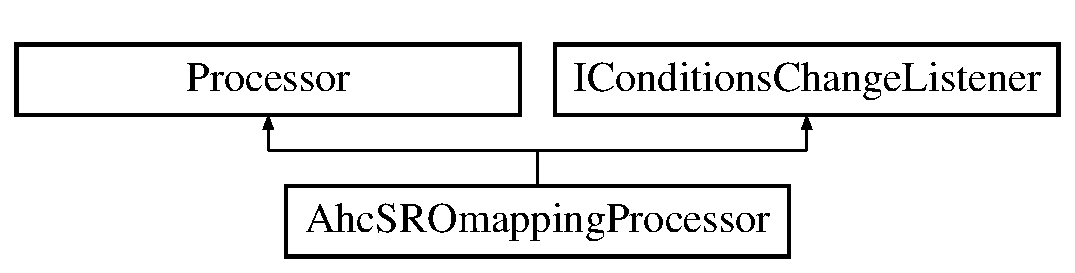
\includegraphics[height=2.000000cm]{classAhcSROmappingProcessor}
\end{center}
\end{figure}
\subsection*{Public Member Functions}
\begin{DoxyCompactItemize}
\item 
virtual Processor $\ast$ {\bfseries new\-Processor} ()\label{classAhcSROmappingProcessor_acdb27fbf3cabcefac542316a507e4ecd}

\item 
virtual void {\bf init} ()
\begin{DoxyCompactList}\small\item\em Called at the begin of the job before anything is read. \end{DoxyCompactList}\item 
virtual void {\bf process\-Event} (L\-C\-Event $\ast$evt)\label{classAhcSROmappingProcessor_a6aed22ae961f2d83301ef5bd3ecbac22}

\begin{DoxyCompactList}\small\item\em Called for every event -\/ the working horse. \end{DoxyCompactList}\item 
virtual void {\bf end} ()\label{classAhcSROmappingProcessor_a1e2654e41cb9d86e674d671e2dffddf8}

\begin{DoxyCompactList}\small\item\em Called after data processing for clean up. \end{DoxyCompactList}\end{DoxyCompactItemize}
\subsection*{Protected Attributes}
\begin{DoxyCompactItemize}
\item 
std\-::string {\bfseries \-\_\-in\-Col\-Name}\label{classAhcSROmappingProcessor_a79fb23db5c3484c5943e6e16f696a4b2}

\item 
std\-::string {\bfseries \-\_\-out\-Col\-Name}\label{classAhcSROmappingProcessor_aea0657c8950e0ebce40bac16f59ec2d8}

\item 
std\-::string {\bfseries \-\_\-mapping\-Col\-Name}\label{classAhcSROmappingProcessor_a0418b9e5c81b0b44fde4b77a7290366f}

\end{DoxyCompactItemize}
\subsection*{Private Member Functions}
\begin{DoxyCompactItemize}
\item 
void {\bfseries conditions\-Changed} (lcio\-::\-L\-C\-Collection $\ast$col)\label{classAhcSROmappingProcessor_ae67481b63f80aba4e19fdd12c4a74da4}

\end{DoxyCompactItemize}
\subsection*{Private Attributes}
\begin{DoxyCompactItemize}
\item 
C\-A\-L\-I\-C\-E\-::\-Ahc\-Slow\-Readout\-Mod\-Mapper {\bfseries \-\_\-mapper}\label{classAhcSROmappingProcessor_a7d712eeff246abd6edd2ecee49fb5777}

\item 
bool {\bfseries \-\_\-mapping\-Changed}\label{classAhcSROmappingProcessor_a8486c29c571d160450e616e6484ee243}

\item 
bool {\bfseries \-\_\-input\-Changed}\label{classAhcSROmappingProcessor_a285e84531df4faeaea3018b8a0a06b32}

\item 
lcio\-::\-L\-C\-Collection $\ast$ {\bfseries \-\_\-mapping\-Col}\label{classAhcSROmappingProcessor_a631ea134f436b99ee520fd705a8d392a}

\item 
lcio\-::\-L\-C\-Collection $\ast$ {\bfseries \-\_\-in\-Col}\label{classAhcSROmappingProcessor_ad60fb94a5944f4575563149537e02feb}

\item 
C\-A\-L\-I\-C\-E\-::\-Run\-Time\-Conditions\-Handler $\ast$ {\bfseries \-\_\-conditions\-Handler}\label{classAhcSROmappingProcessor_a13e326e568c0a3ba6b6b4fe6cfca5ab1}

\item 
bool {\bfseries \-\_\-mapping\-Available}\label{classAhcSROmappingProcessor_a33de2e4f529735385931b547914446b2}

\item 
lcio\-::\-L\-C\-Collection $\ast$ {\bfseries \-\_\-last\-Data\-Col}\label{classAhcSROmappingProcessor_a0df24f16b476f7d484caefc258294e5a}

\end{DoxyCompactItemize}


\subsection{Detailed Description}
Processor to fix the mapping of a collection of Ahc\-Slow\-Readout\-Mod\-Block. 

This processor retrieves the data by Conditions\-Change\-Listener for the input-\/ and mapping-\/collection.

The output is added to the event by a Run\-Time\-Conditions\-Handler to propagate the change to possible further Conditions\-Change\-Listener.

\begin{DoxySeeAlso}{See Also}
lccd\-::\-I\-Conditions\-Change\-Listener 

C\-A\-L\-I\-C\-E\-::\-Run\-Time\-Conditions\-Handler 

marlin\-::\-Conditions\-Processor
\end{DoxySeeAlso}
\begin{DoxyAuthor}{Author}
{\tt Benjamin.\-Lutz@desy.\-de} 
\end{DoxyAuthor}
\begin{DoxyDate}{Date}
Dec 2008 
\end{DoxyDate}
\begin{DoxyVersion}{Version}
1.\-0 
\end{DoxyVersion}


Definition at line 30 of file Ahc\-S\-R\-Omapping\-Processor.\-hh.



\subsection{Member Function Documentation}
\index{Ahc\-S\-R\-Omapping\-Processor@{Ahc\-S\-R\-Omapping\-Processor}!init@{init}}
\index{init@{init}!AhcSROmappingProcessor@{Ahc\-S\-R\-Omapping\-Processor}}
\subsubsection[{init}]{\setlength{\rightskip}{0pt plus 5cm}void Ahc\-S\-R\-Omapping\-Processor\-::init (
\begin{DoxyParamCaption}
{}
\end{DoxyParamCaption}
)\hspace{0.3cm}{\ttfamily [virtual]}}\label{classAhcSROmappingProcessor_a4b86cdb371c629d8a5919c5ddedb60d5}


Called at the begin of the job before anything is read. 

Use to initialize the processor, e.\-g. book histograms. 

Definition at line 44 of file Ahc\-S\-R\-Omapping\-Processor.\-cc.



The documentation for this class was generated from the following files\-:\begin{DoxyCompactItemize}
\item 
Ahc\-S\-R\-Omapping\-Processor.\-hh\item 
Ahc\-S\-R\-Omapping\-Processor.\-cc\end{DoxyCompactItemize}

\section{T\-B\-Track\-:\-:Aln\-Constants Class Reference}
\label{classTBTrack_1_1AlnConstants}\index{T\-B\-Track\-::\-Aln\-Constants@{T\-B\-Track\-::\-Aln\-Constants}}
Inheritance diagram for T\-B\-Track\-:\-:Aln\-Constants\-:\begin{figure}[H]
\begin{center}
\leavevmode
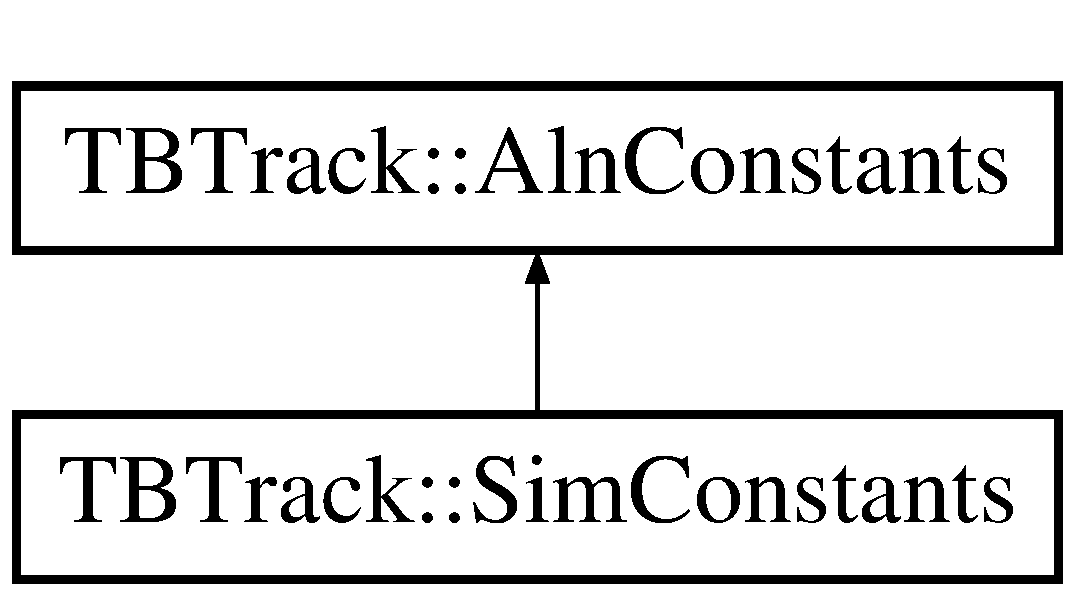
\includegraphics[height=2.000000cm]{classTBTrack_1_1AlnConstants}
\end{center}
\end{figure}
\subsection*{Public Types}
\begin{DoxyCompactItemize}
\item 
enum \{ {\bfseries number\-Of\-Ints} =0
 \}
\item 
enum \{ {\bfseries number\-Of\-Floats} =0
 \}
\item 
enum \{ {\bfseries number\-Of\-Doubles} =1+3$\ast$2$\ast$4
 \}
\end{DoxyCompactItemize}
\subsection*{Public Member Functions}
\begin{DoxyCompactItemize}
\item 
{\bfseries Aln\-Constants} (int period=0, int data\-Type=2)\label{classTBTrack_1_1AlnConstants_af91893338898d5c5d60add694f7ad53c}

\item 
double {\bfseries tdc\-Unit} () const \label{classTBTrack_1_1AlnConstants_af8ecb4ff47971cea86ea57719657405d}

\item 
void {\bfseries tdc\-Unit} (double t)\label{classTBTrack_1_1AlnConstants_a1070adc84db54a491c8ead531aa74bfe}

\item 
double {\bfseries c\-Tzero} (unsigned d, unsigned l) const \label{classTBTrack_1_1AlnConstants_a92e168a711778633d7629411f6567ec6}

\item 
void {\bfseries c\-Tzero} (unsigned d, unsigned l, double c)\label{classTBTrack_1_1AlnConstants_a02360b72db926a833aa6883221bb25c1}

\item 
double {\bfseries v\-Drift} (unsigned d, unsigned l) const \label{classTBTrack_1_1AlnConstants_a3e0815db478c533f423c090090ac7f58}

\item 
void {\bfseries v\-Drift} (unsigned d, unsigned l, double v)\label{classTBTrack_1_1AlnConstants_ab1801a04e89c0d92726ebaf82da6c7ea}

\item 
double {\bfseries v\-Dquad} (unsigned d, unsigned l) const \label{classTBTrack_1_1AlnConstants_a502d35c057f8703828a8c4772c981372}

\item 
void {\bfseries v\-Dquad} (unsigned d, unsigned l, double q)\label{classTBTrack_1_1AlnConstants_a69529ea7d72f1d98029aa479ef5f94a6}

\item 
double {\bfseries coordinate} (unsigned d, unsigned l, int t) const \label{classTBTrack_1_1AlnConstants_a4248f4f0634ada340af67a1e5129c5dc}

\item 
int {\bfseries tdc\-Value} (unsigned d, unsigned l, double c, double t=0.\-0) const \label{classTBTrack_1_1AlnConstants_aa51d47ab24355ca238e1e79ff8acf053}

\item 
std\-::ostream \& {\bfseries print} (std\-::ostream \&o=std\-::cout, const std\-::string \&s=\char`\"{}\char`\"{}) const \label{classTBTrack_1_1AlnConstants_aa01bb46450b492761c90392eb81411bc}

\item 
const int $\ast$ {\bfseries int\-Data} () const \label{classTBTrack_1_1AlnConstants_afb793481bc8c9ea4786e9e52144cb708}

\item 
int $\ast$ {\bfseries int\-Data} ()\label{classTBTrack_1_1AlnConstants_a5ffc45d080fe15974fca534ae01c3146}

\item 
const float $\ast$ {\bfseries float\-Data} () const \label{classTBTrack_1_1AlnConstants_a2d50c758aa6c1a6bbfa4790d7c1d1ed1}

\item 
float $\ast$ {\bfseries float\-Data} ()\label{classTBTrack_1_1AlnConstants_a48b746d9e7043bd80d2968bed18f21ef}

\item 
const double $\ast$ {\bfseries double\-Data} () const \label{classTBTrack_1_1AlnConstants_afd83d2588465d22b8ef17cb39326ee5b}

\item 
double $\ast$ {\bfseries double\-Data} ()\label{classTBTrack_1_1AlnConstants_aa07f0bb0b3cdde7eb56afa7050e626d9}

\end{DoxyCompactItemize}
\subsection*{Protected Attributes}
\begin{DoxyCompactItemize}
\item 
double {\bfseries \-\_\-tdc\-Unit}\label{classTBTrack_1_1AlnConstants_a2cf1c1f9615a86de4d37f9a72ff0292b}

\item 
double {\bfseries \-\_\-c\-Tzero} [2][4]\label{classTBTrack_1_1AlnConstants_af55cc6424803c2d11d027bcec1b64f82}

\item 
double {\bfseries \-\_\-v\-Drift} [2][4]\label{classTBTrack_1_1AlnConstants_a31dab51bbeacb52b53f8d1bc2cd2466a}

\item 
double {\bfseries \-\_\-v\-Dquad} [2][4]\label{classTBTrack_1_1AlnConstants_a91b9a4fcb791b1a3aeade9408633bbcf}

\end{DoxyCompactItemize}


\subsection{Detailed Description}


Definition at line 16 of file Aln\-Constants.\-hh.



The documentation for this class was generated from the following files\-:\begin{DoxyCompactItemize}
\item 
Aln\-Constants.\-hh\item 
Aln\-Constants.\-cc\end{DoxyCompactItemize}

\section{C\-A\-L\-I\-C\-E\-:\-:Append\-Multi\-Amplitude Class Reference}
\label{classCALICE_1_1AppendMultiAmplitude}\index{C\-A\-L\-I\-C\-E\-::\-Append\-Multi\-Amplitude@{C\-A\-L\-I\-C\-E\-::\-Append\-Multi\-Amplitude}}


Processor to add P\-A\-R\-\_\-\-M\-U\-L\-T\-I\-\_\-\-A\-M\-P\-L (amplitude of the Multiplicity Counter) to the event.  




{\ttfamily \#include $<$Append\-Multi\-Amplitude.\-hh$>$}

Inheritance diagram for C\-A\-L\-I\-C\-E\-:\-:Append\-Multi\-Amplitude\-:\begin{figure}[H]
\begin{center}
\leavevmode
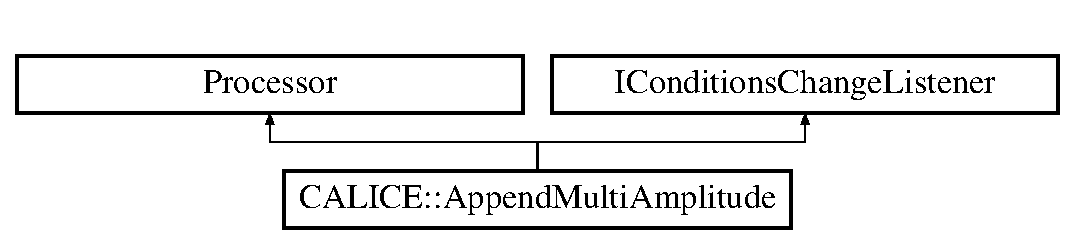
\includegraphics[height=2.000000cm]{classCALICE_1_1AppendMultiAmplitude}
\end{center}
\end{figure}
\subsection*{Public Member Functions}
\begin{DoxyCompactItemize}
\item 
Processor $\ast$ {\bfseries new\-Processor} ()\label{classCALICE_1_1AppendMultiAmplitude_af5c8a3fce4bc7612157e3d6ad50872d6}

\item 
void {\bfseries init} ()\label{classCALICE_1_1AppendMultiAmplitude_a528565bad5c83a2677bc752f4d47d1f6}

\item 
void {\bfseries process\-Run\-Header} (L\-C\-Run\-Header $\ast$run)\label{classCALICE_1_1AppendMultiAmplitude_a6c147a934e7b60ecbf788f7de33bfde9}

\item 
void {\bfseries process\-Event} (L\-C\-Event $\ast$evt)\label{classCALICE_1_1AppendMultiAmplitude_a80b214680c8275820126d7826b2ca0e0}

\item 
void {\bfseries end} ()\label{classCALICE_1_1AppendMultiAmplitude_a9976e1ce7c039db675881af775f68986}

\end{DoxyCompactItemize}
\subsection*{Protected Attributes}
\begin{DoxyCompactItemize}
\item 
std\-::string {\bfseries \-\_\-adc\-Col\-Name}\label{classCALICE_1_1AppendMultiAmplitude_a90acd521e292e3f2bdd9ff56b4606f55}

\item 
std\-::string {\bfseries \-\_\-connection\-Col\-Name}\label{classCALICE_1_1AppendMultiAmplitude_a2902a95068d152cb11826aafe85f63bb}

\item 
std\-::string {\bfseries \-\_\-par\-Name\-Multi\-Ampl}\label{classCALICE_1_1AppendMultiAmplitude_a209412842c94a4ff6be9af6f7b41bf89}

\end{DoxyCompactItemize}
\subsection*{Private Member Functions}
\begin{DoxyCompactItemize}
\item 
void {\bfseries conditions\-Changed} (lcio\-::\-L\-C\-Collection $\ast$col)\label{classCALICE_1_1AppendMultiAmplitude_ae04c6bc30a5a1bfc4700c2575ae09a76}

\end{DoxyCompactItemize}
\subsection*{Private Attributes}
\begin{DoxyCompactItemize}
\item 
unsigned int {\bfseries \-\_\-crate}\label{classCALICE_1_1AppendMultiAmplitude_a4ecf8796bb93026dbf2d680b7dd70214}

\item 
unsigned int {\bfseries \-\_\-slot}\label{classCALICE_1_1AppendMultiAmplitude_a281f76046ded3a3aa7c5880242caf1bd}

\item 
unsigned int {\bfseries \-\_\-fe}\label{classCALICE_1_1AppendMultiAmplitude_a0b02671cdf754fc52ab8fa6348293431}

\item 
unsigned int {\bfseries \-\_\-chip}\label{classCALICE_1_1AppendMultiAmplitude_aa15678d8ba0780fad8c59e546087781d}

\item 
unsigned int {\bfseries \-\_\-channel}\label{classCALICE_1_1AppendMultiAmplitude_ab205e6309046702fb743238a594a14fd}

\item 
bool {\bfseries \-\_\-connection\-Available}\label{classCALICE_1_1AppendMultiAmplitude_af350bb41fd000d9968f9097cb91ad771}

\end{DoxyCompactItemize}


\subsection{Detailed Description}
Processor to add P\-A\-R\-\_\-\-M\-U\-L\-T\-I\-\_\-\-A\-M\-P\-L (amplitude of the Multiplicity Counter) to the event. 

This processor adds an event parameter containing the amplitude of the analog multiplicity counter readout. The mapping of the multiplicity counter connection is read from the L\-C\-I\-O stream.

\begin{DoxyVersion}{Version}
1.\-0 
\end{DoxyVersion}
\begin{DoxyAuthor}{Author}
{\tt Benjamin.\-Lutz@desy.\-de} 

{\tt Nils.\-Feege@desy.\-de} 
\end{DoxyAuthor}
\begin{DoxyDate}{Date}
March 2010 
\end{DoxyDate}


Definition at line 25 of file Append\-Multi\-Amplitude.\-hh.



The documentation for this class was generated from the following files\-:\begin{DoxyCompactItemize}
\item 
Append\-Multi\-Amplitude.\-hh\item 
Append\-Multi\-Amplitude.\-cc\end{DoxyCompactItemize}

\section{C\-A\-L\-I\-C\-E\-:\-:Average\-History\-Graphs Class Reference}
\label{classCALICE_1_1AverageHistoryGraphs}\index{C\-A\-L\-I\-C\-E\-::\-Average\-History\-Graphs@{C\-A\-L\-I\-C\-E\-::\-Average\-History\-Graphs}}
Inheritance diagram for C\-A\-L\-I\-C\-E\-:\-:Average\-History\-Graphs\-:\begin{figure}[H]
\begin{center}
\leavevmode
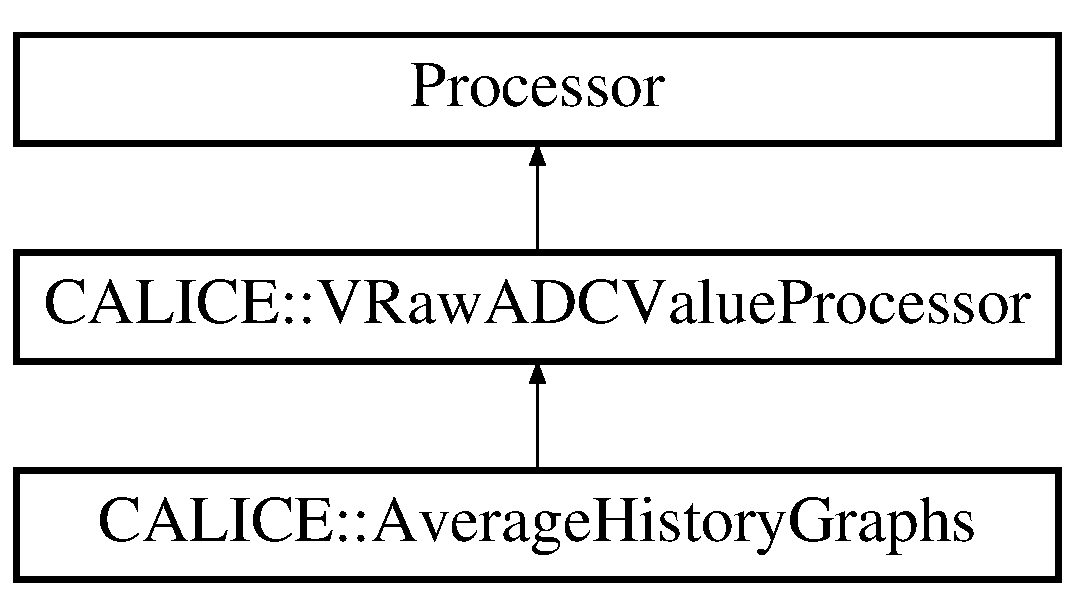
\includegraphics[height=3.000000cm]{classCALICE_1_1AverageHistoryGraphs}
\end{center}
\end{figure}
\subsection*{Public Member Functions}
\begin{DoxyCompactItemize}
\item 
Processor $\ast$ {\bfseries new\-Processor} ()\label{classCALICE_1_1AverageHistoryGraphs_aadeafdb3a9c7e2f355af43bbe2600a36}

\item 
void {\bf init} ()
\begin{DoxyCompactList}\small\item\em Called at the begin of the job before anything is read. \end{DoxyCompactList}\item 
void {\bf process\-Run\-Header} (L\-C\-Run\-Header $\ast$run)
\begin{DoxyCompactList}\small\item\em Called for every run, e.\-g. \end{DoxyCompactList}\item 
void {\bf process\-Event} (L\-C\-Event $\ast$evt\-P)
\begin{DoxyCompactList}\small\item\em Called for every event -\/ the working horse. \end{DoxyCompactList}\item 
void {\bfseries end} ()\label{classCALICE_1_1AverageHistoryGraphs_a66fdedb6f7f91bc59a2c5acb73d9e500}

\end{DoxyCompactItemize}
\subsection*{Protected Types}
\begin{DoxyCompactItemize}
\item 
enum {\bfseries E\-Graph\-Type} \{ \\*
{\bfseries k\-Graph\-Mean}, 
{\bfseries k\-Graph\-R\-M\-S}, 
{\bfseries k\-Graph\-Min}, 
{\bfseries k\-Graph\-Max}, 
\\*
{\bfseries k\-Graph\-Weight}, 
{\bfseries k\-N\-Graph\-Types}
 \}
\item 
enum {\bfseries E\-History\-Type} \{ \\*
{\bfseries k\-A\-D\-C\-History}, 
{\bfseries k\-Noise\-History}, 
{\bfseries k\-Pedestal\-History}, 
{\bfseries k\-Hit\-History}, 
\\*
{\bfseries k\-N\-History\-Graphs}
 \}
\item 
enum {\bfseries E\-Stamp\-Type} \{ \\*
{\bfseries k\-History\-Stamp}, 
{\bfseries k\-History\-Conf\-Stamp}, 
{\bfseries k\-History\-State\-Stamp}, 
{\bfseries k\-History\-State\-Value}, 
\\*
{\bfseries k\-N\-History\-Stamps}
 \}
\end{DoxyCompactItemize}
\subsection*{Protected Member Functions}
\begin{DoxyCompactItemize}
\item 
void {\bfseries configuration\-Changed} (E\-V\-E\-N\-T\-::\-L\-C\-Collection $\ast$)\label{classCALICE_1_1AverageHistoryGraphs_a176525151e7d59d850f171befa7d793b}

\item 
void {\bfseries module\-Type\-Changed} (lcio\-::\-L\-C\-Collection $\ast$col)\label{classCALICE_1_1AverageHistoryGraphs_acdba66e246541547c5fb4ba032e4c781}

\item 
void {\bfseries module\-Location\-Changed} (lcio\-::\-L\-C\-Collection $\ast$col)\label{classCALICE_1_1AverageHistoryGraphs_ab2da21acfb64312a3182becc51232998}

\item 
void {\bfseries module\-Connection\-Changed} (lcio\-::\-L\-C\-Collection $\ast$col)\label{classCALICE_1_1AverageHistoryGraphs_a126a4d42d653c4c005a5135d0dfea159}

\item 
void {\bfseries resize\-Arrays} ()\label{classCALICE_1_1AverageHistoryGraphs_a1f1586ff5a3fe049d6613a296128bbcd}

\end{DoxyCompactItemize}
\subsection*{Protected Attributes}
\begin{DoxyCompactItemize}
\item 
Int\-\_\-t {\bfseries \-\_\-use\-Time\-Stamp}\label{classCALICE_1_1AverageHistoryGraphs_a924519564a5a56335cc071811de29594}

\item 
Int\-Vec {\bfseries \-\_\-event\-Par}\label{classCALICE_1_1AverageHistoryGraphs_a9cd19052bd65b4925f23feaa915086c3}

\item 
Int\-\_\-t {\bfseries \-\_\-av\-A\-D\-C\-N\-Max}\label{classCALICE_1_1AverageHistoryGraphs_aaea631c4dde12b4da4274e9028b5bfa8}

\item 
Float\-\_\-t {\bfseries \-\_\-signal\-Cut}\label{classCALICE_1_1AverageHistoryGraphs_abe695f79dbd74292894bc9e8b53a3324}

\item 
Int\-\_\-t {\bfseries \-\_\-skip\-Calibration\-Events\-Always}\label{classCALICE_1_1AverageHistoryGraphs_a83a1b6b057c3e5c5b01aea6442864ed5}

\item 
std\-::string {\bfseries \-\_\-cell\-Parameter\-Collection\-Name}\label{classCALICE_1_1AverageHistoryGraphs_a1eca22a5971a5a7d480ae8f9c14f74fb}

\item 
std\-::vector$<$ std\-::vector\\*
$<$ Average\-\_\-t $>$ $>$ {\bfseries \-\_\-av\-Values} [k\-N\-History\-Graphs]\label{classCALICE_1_1AverageHistoryGraphs_ae0b1ef124d0704af661c3a6cff2c793a}

\item 
bool {\bfseries \-\_\-av\-A\-D\-C\-Is\-Valid}\label{classCALICE_1_1AverageHistoryGraphs_ac8f0ccd575282d74f9239f93e662faf7}

\item 
U\-Int\-\_\-t {\bfseries \-\_\-av\-A\-D\-Cn}\label{classCALICE_1_1AverageHistoryGraphs_adcdef8bfa777ecd9977e6e4c03b6177b}

\item 
std\-::vector$<$ std\-::vector\\*
$<$ Average\-\_\-t $>$ $>$ {\bfseries \-\_\-av\-A\-D\-C}\label{classCALICE_1_1AverageHistoryGraphs_a09f9a1eb99e16951c1bb2219690d0332}

\item 
std\-::vector$<$ std\-::vector\\*
$<$ U\-Int\-\_\-t $>$ $>$ {\bfseries \-\_\-n\-Hits}\label{classCALICE_1_1AverageHistoryGraphs_a9ac965b72b8eaf330366d65ca3e6bb40}

\item 
String\-Vec {\bfseries \-\_\-monitor\-Conf}\label{classCALICE_1_1AverageHistoryGraphs_a98da6d927a6ed04dc03e91057181912c}

\item 
vector\\*
$<$ Conditions\-Change\-Delegator\\*
$<$ {\bf Average\-History\-Graphs} $>$ $>$ {\bfseries \-\_\-conf\-Changes}\label{classCALICE_1_1AverageHistoryGraphs_a03616ae3f8232db9aa14cbd67332cfe1}

\item 
bool {\bfseries \-\_\-conf\-Changed}\label{classCALICE_1_1AverageHistoryGraphs_acd099e4c900efbc66f69f8cce8391f03}

\item 
U\-Int\-\_\-t {\bfseries \-\_\-n\-Configuration\-Changes}\label{classCALICE_1_1AverageHistoryGraphs_aa18f88276066de50377761e7ce983cba}

\item 
Int\-\_\-t {\bfseries \-\_\-was\-State}\label{classCALICE_1_1AverageHistoryGraphs_a8cc7262ec5a99b0562f812fd014a1c26}

\item 
U\-Int\-\_\-t {\bfseries \-\_\-n\-State\-Changes}\label{classCALICE_1_1AverageHistoryGraphs_adbc2ad77c6f5945a98131e4af3cbd2ef}

\item 
{\bf histmgr\-::\-Key\-\_\-t} {\bfseries \-\_\-graph\-Group\-Key}\label{classCALICE_1_1AverageHistoryGraphs_a5b92eb7bf713fc38bb4ab6a033477be6}

\item 
std\-::vector$<$ {\bf histmgr\-::\-Key\-\_\-t} $>$ {\bfseries \-\_\-av\-Value\-History\-Key}\label{classCALICE_1_1AverageHistoryGraphs_a9b71e2d36930c41347fe49a0e8495b7d}

\item 
{\bf histmgr\-::\-Key\-\_\-t} {\bfseries \-\_\-state\-Change\-History\-Key}\label{classCALICE_1_1AverageHistoryGraphs_a1f003a748d898ea24d416211dd8b9168}

\item 
{\bf histmgr\-::\-Key\-\_\-t} {\bfseries \-\_\-conf\-Change\-History\-Key}\label{classCALICE_1_1AverageHistoryGraphs_af654242bdda2b428ba576813b6d46559}

\end{DoxyCompactItemize}
\subsection*{Static Protected Attributes}
\begin{DoxyCompactItemize}
\item 
static const char $\ast$ {\bfseries \-\_\-\-\_\-graph\-Type\-Names} [k\-N\-Graph\-Types]
\item 
static const char $\ast$ {\bfseries \-\_\-\-\_\-history\-Graph\-Names} [k\-N\-History\-Graphs]
\item 
static U\-Int\-\_\-t {\bfseries \-\_\-\-\_\-n\-Samples\-Per\-Chip} =18\label{classCALICE_1_1AverageHistoryGraphs_a38373d247acaed96390b500046c523ac}

\item 
static U\-Int\-\_\-t {\bfseries \-\_\-\-\_\-n\-Chips} =12\label{classCALICE_1_1AverageHistoryGraphs_a376afe7cdb43b7a1ed6be6cdcfbc9bb5}

\end{DoxyCompactItemize}


\subsection{Detailed Description}


Definition at line 17 of file Average\-History\-Graphs.\-hh.



\subsection{Member Function Documentation}
\index{C\-A\-L\-I\-C\-E\-::\-Average\-History\-Graphs@{C\-A\-L\-I\-C\-E\-::\-Average\-History\-Graphs}!init@{init}}
\index{init@{init}!CALICE::AverageHistoryGraphs@{C\-A\-L\-I\-C\-E\-::\-Average\-History\-Graphs}}
\subsubsection[{init}]{\setlength{\rightskip}{0pt plus 5cm}void C\-A\-L\-I\-C\-E\-::\-Average\-History\-Graphs\-::init (
\begin{DoxyParamCaption}
{}
\end{DoxyParamCaption}
)}\label{classCALICE_1_1AverageHistoryGraphs_a3734a824ecbe14585605e459c40b7f67}


Called at the begin of the job before anything is read. 

Use to initialize the processor, e.\-g. book histograms. 

Definition at line 121 of file Average\-History\-Graphs.\-cc.



References histmgr\-::\-Hist\-Mgr\-::create\-Graph\-Collection(), histmgr\-::\-Hist\-Mgr\-::create\-Histogram\-Group(), and histmgr\-::\-Hist\-Mgr\-::lock\-Group().

\index{C\-A\-L\-I\-C\-E\-::\-Average\-History\-Graphs@{C\-A\-L\-I\-C\-E\-::\-Average\-History\-Graphs}!process\-Event@{process\-Event}}
\index{process\-Event@{process\-Event}!CALICE::AverageHistoryGraphs@{C\-A\-L\-I\-C\-E\-::\-Average\-History\-Graphs}}
\subsubsection[{process\-Event}]{\setlength{\rightskip}{0pt plus 5cm}void C\-A\-L\-I\-C\-E\-::\-Average\-History\-Graphs\-::process\-Event (
\begin{DoxyParamCaption}
\item[{L\-C\-Event $\ast$}]{evt\-P}
\end{DoxyParamCaption}
)}\label{classCALICE_1_1AverageHistoryGraphs_a1b70e2c0f46158aac6fe28edb2ca23cf}


Called for every event -\/ the working horse. 



Definition at line 251 of file Average\-History\-Graphs.\-cc.



References C\-A\-L\-I\-C\-E\-::\-V\-Raw\-A\-D\-C\-Value\-Processor\-::\-\_\-adc\-Col\-Name, histmgr\-::\-Graph\-Collection\-\_\-t\-::append\-X\-Value(), histmgr\-::\-Hist\-Mgr\-::get\-Graph\-Collection(), C\-A\-L\-I\-C\-E\-::\-Cell\-Parameter\-::get\-Noise(), C\-A\-L\-I\-C\-E\-::\-Cell\-Parameter\-::get\-Pedestal(), and histmgr\-::\-Graph\-Collection\-\_\-t\-::set\-Y\-Value().

\index{C\-A\-L\-I\-C\-E\-::\-Average\-History\-Graphs@{C\-A\-L\-I\-C\-E\-::\-Average\-History\-Graphs}!process\-Run\-Header@{process\-Run\-Header}}
\index{process\-Run\-Header@{process\-Run\-Header}!CALICE::AverageHistoryGraphs@{C\-A\-L\-I\-C\-E\-::\-Average\-History\-Graphs}}
\subsubsection[{process\-Run\-Header}]{\setlength{\rightskip}{0pt plus 5cm}void C\-A\-L\-I\-C\-E\-::\-Average\-History\-Graphs\-::process\-Run\-Header (
\begin{DoxyParamCaption}
\item[{L\-C\-Run\-Header $\ast$}]{run}
\end{DoxyParamCaption}
)\hspace{0.3cm}{\ttfamily [inline]}}\label{classCALICE_1_1AverageHistoryGraphs_a0b55ddfdfa8bac7bc5f17cd94c695da6}


Called for every run, e.\-g. 

overwrite to initialize run dependent histograms. 

Definition at line 34 of file Average\-History\-Graphs.\-hh.



\subsection{Field Documentation}
\index{C\-A\-L\-I\-C\-E\-::\-Average\-History\-Graphs@{C\-A\-L\-I\-C\-E\-::\-Average\-History\-Graphs}!\-\_\-\-\_\-graph\-Type\-Names@{\-\_\-\-\_\-graph\-Type\-Names}}
\index{\-\_\-\-\_\-graph\-Type\-Names@{\-\_\-\-\_\-graph\-Type\-Names}!CALICE::AverageHistoryGraphs@{C\-A\-L\-I\-C\-E\-::\-Average\-History\-Graphs}}
\subsubsection[{\-\_\-\-\_\-graph\-Type\-Names}]{\setlength{\rightskip}{0pt plus 5cm}const char $\ast$ C\-A\-L\-I\-C\-E\-::\-Average\-History\-Graphs\-::\-\_\-\-\_\-graph\-Type\-Names\hspace{0.3cm}{\ttfamily [static]}, {\ttfamily [protected]}}\label{classCALICE_1_1AverageHistoryGraphs_adce732f8a36e6b716ab80ff035b2603a}
{\bfseries Initial value\-:}
\begin{DoxyCode}
=\{
    \textcolor{stringliteral}{"mean"},
    \textcolor{stringliteral}{"rms"},
    \textcolor{stringliteral}{"min"},
    \textcolor{stringliteral}{"max"},
    \textcolor{stringliteral}{"weight"}
  \}
\end{DoxyCode}


Definition at line 61 of file Average\-History\-Graphs.\-hh.

\index{C\-A\-L\-I\-C\-E\-::\-Average\-History\-Graphs@{C\-A\-L\-I\-C\-E\-::\-Average\-History\-Graphs}!\-\_\-\-\_\-history\-Graph\-Names@{\-\_\-\-\_\-history\-Graph\-Names}}
\index{\-\_\-\-\_\-history\-Graph\-Names@{\-\_\-\-\_\-history\-Graph\-Names}!CALICE::AverageHistoryGraphs@{C\-A\-L\-I\-C\-E\-::\-Average\-History\-Graphs}}
\subsubsection[{\-\_\-\-\_\-history\-Graph\-Names}]{\setlength{\rightskip}{0pt plus 5cm}const char $\ast$ C\-A\-L\-I\-C\-E\-::\-Average\-History\-Graphs\-::\-\_\-\-\_\-history\-Graph\-Names\hspace{0.3cm}{\ttfamily [static]}, {\ttfamily [protected]}}\label{classCALICE_1_1AverageHistoryGraphs_a2349f46d366705d3d312fbc32febf896}
{\bfseries Initial value\-:}
\begin{DoxyCode}
=\{
    \textcolor{stringliteral}{"ADCHistory"},
    \textcolor{stringliteral}{"NoiseHistory"},
    \textcolor{stringliteral}{"PedestalHistory"},
    \textcolor{stringliteral}{"HitHistory"}
  \}
\end{DoxyCode}


Definition at line 62 of file Average\-History\-Graphs.\-hh.



The documentation for this class was generated from the following files\-:\begin{DoxyCompactItemize}
\item 
Average\-History\-Graphs.\-hh\item 
Average\-History\-Graphs.\-cc\end{DoxyCompactItemize}

\section{C\-A\-L\-I\-C\-E\-:\-:Base\-Mapping\-I\-I\-Processor Class Reference}
\label{classCALICE_1_1BaseMappingIIProcessor}\index{C\-A\-L\-I\-C\-E\-::\-Base\-Mapping\-I\-I\-Processor@{C\-A\-L\-I\-C\-E\-::\-Base\-Mapping\-I\-I\-Processor}}
Inheritance diagram for C\-A\-L\-I\-C\-E\-:\-:Base\-Mapping\-I\-I\-Processor\-:\begin{figure}[H]
\begin{center}
\leavevmode
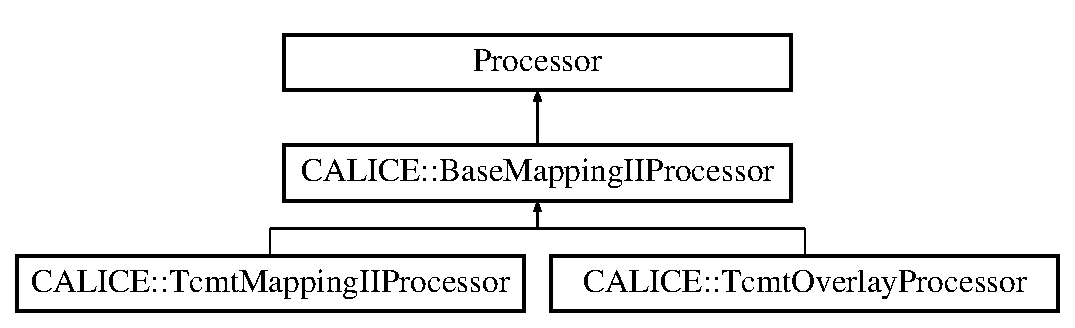
\includegraphics[height=3.000000cm]{classCALICE_1_1BaseMappingIIProcessor}
\end{center}
\end{figure}
\subsection*{Public Member Functions}
\begin{DoxyCompactItemize}
\item 
{\bfseries Base\-Mapping\-I\-I\-Processor} (const std\-::string \&type\-Name)\label{classCALICE_1_1BaseMappingIIProcessor_a8fe56d91380e26a12371e14a323d25d6}

\item 
virtual void {\bfseries init} ()\label{classCALICE_1_1BaseMappingIIProcessor_abb1ef572435bcc64898506d8f4c96cd9}

\item 
virtual void {\bfseries process\-Run\-Header} (L\-C\-Run\-Header $\ast$run)\label{classCALICE_1_1BaseMappingIIProcessor_a995afff29900be06e93ebe0453ed4aa6}

\item 
virtual void {\bfseries process\-Event} (L\-C\-Event $\ast$evt)=0\label{classCALICE_1_1BaseMappingIIProcessor_a5ac01e2e7f361f7ec4e1bd039ccbd33b}

\item 
virtual void {\bfseries check} (L\-C\-Event $\ast$evt)\label{classCALICE_1_1BaseMappingIIProcessor_a4abb713a96256ee6599e9737e54bdfe1}

\item 
virtual void {\bfseries end} ()\label{classCALICE_1_1BaseMappingIIProcessor_a201450aeeedac3600901e6fd1d25ada6}

\end{DoxyCompactItemize}
\subsection*{Protected Member Functions}
\begin{DoxyCompactItemize}
\item 
virtual void {\bfseries update\-Inverse\-Map} ()\label{classCALICE_1_1BaseMappingIIProcessor_a60b39bae8ec80110e15b126c77138103}

\item 
virtual void {\bfseries module\-Type\-Changed} (lcio\-::\-L\-C\-Collection $\ast$col)\label{classCALICE_1_1BaseMappingIIProcessor_a016f786152f13a2dbb7a0ca9c0727a08}

\item 
virtual void {\bfseries module\-Location\-Changed} (lcio\-::\-L\-C\-Collection $\ast$col)\label{classCALICE_1_1BaseMappingIIProcessor_a9b65e70f55abef48ee724dab92c2b5db}

\item 
virtual void {\bfseries module\-Connection\-Changed} (lcio\-::\-L\-C\-Collection $\ast$col)\label{classCALICE_1_1BaseMappingIIProcessor_a4ea22fa131cd52bdb59a9dc0d49bb033}

\item 
virtual void {\bfseries detector\-Transformation\-Changed} (lcio\-::\-L\-C\-Collection $\ast$col)\label{classCALICE_1_1BaseMappingIIProcessor_ac82c048d8b7e3f28fe3b17b4855bb989}

\item 
virtual void {\bfseries reference\-Transformation\-Changed} (lcio\-::\-L\-C\-Collection $\ast$col)\label{classCALICE_1_1BaseMappingIIProcessor_a5e17c0ecedbbb704f21f94091aeb61f0}

\end{DoxyCompactItemize}
\subsection*{Protected Attributes}
\begin{DoxyCompactItemize}
\item 
std\-::string {\bfseries \-\_\-input\-Col\-Name}\label{classCALICE_1_1BaseMappingIIProcessor_a89f87c70722b470ce3351a1a94a04c5d}

\item 
std\-::string {\bfseries \-\_\-output\-Col\-Name}\label{classCALICE_1_1BaseMappingIIProcessor_a55c4612d6057c09ccabb5bce43cfd184}

\item 
std\-::string {\bfseries \-\_\-col\-Name\-Module\-Description}\label{classCALICE_1_1BaseMappingIIProcessor_a3cf654ae79db0b075343f05f66b86974}

\item 
std\-::string {\bfseries \-\_\-col\-Name\-Module\-Location}\label{classCALICE_1_1BaseMappingIIProcessor_a2ca5ef0fe54cf330a00b5a89fe7baacf}

\item 
std\-::string {\bfseries \-\_\-col\-Name\-Module\-Connection}\label{classCALICE_1_1BaseMappingIIProcessor_a0a03a8f94ec07d56db8cb88174fe72cd}

\item 
std\-::string {\bfseries \-\_\-col\-Name\-Detector\-Transformation}\label{classCALICE_1_1BaseMappingIIProcessor_aed612620eab1d8ebeb5a584826f70781}

\item 
std\-::string {\bfseries \-\_\-col\-Name\-Reference\-Transformation}\label{classCALICE_1_1BaseMappingIIProcessor_a944b28e0d8de4b183e9dced0d24aa863}

\item 
Conditions\-Change\-Delegator\\*
$<$ {\bf Base\-Mapping\-I\-I\-Processor} $>$ {\bfseries \-\_\-module\-Type\-Change}\label{classCALICE_1_1BaseMappingIIProcessor_aec48652f1896782024ba9cf85eaeb0f9}

\item 
Conditions\-Change\-Delegator\\*
$<$ {\bf Base\-Mapping\-I\-I\-Processor} $>$ {\bfseries \-\_\-module\-Location\-Change}\label{classCALICE_1_1BaseMappingIIProcessor_abbc58227157b9c1c293845f46e41b37a}

\item 
Conditions\-Change\-Delegator\\*
$<$ {\bf Base\-Mapping\-I\-I\-Processor} $>$ {\bfseries \-\_\-module\-Connection\-Change}\label{classCALICE_1_1BaseMappingIIProcessor_a862d6f636084c8a5b97a3d325aaf9115}

\item 
Conditions\-Change\-Delegator\\*
$<$ {\bf Base\-Mapping\-I\-I\-Processor} $>$ {\bfseries \-\_\-detector\-Transformation\-Change}\label{classCALICE_1_1BaseMappingIIProcessor_abd2368662503bb079b2e60e10c5ff77f}

\item 
Conditions\-Change\-Delegator\\*
$<$ {\bf Base\-Mapping\-I\-I\-Processor} $>$ {\bfseries \-\_\-reference\-Transformation\-Change}\label{classCALICE_1_1BaseMappingIIProcessor_a265f357118f9770bf12edf8c4144338f}

\item 
Mapping\-And\-Alignment {\bfseries \-\_\-mapping}\label{classCALICE_1_1BaseMappingIIProcessor_a41bfff962f24cc68687dcf4b482db560}

\item 
bool {\bfseries \-\_\-view\-Connection\-Tree}\label{classCALICE_1_1BaseMappingIIProcessor_ae06d06bfae0591fb5f89b749f476af13}

\item 
std\-::map$<$ unsigned, unsigned $>$ {\bfseries \-\_\-inverse\-Module\-Map}\label{classCALICE_1_1BaseMappingIIProcessor_aa4baf288fa623c98ec56a5c97e2b6b08}

\end{DoxyCompactItemize}


\subsection{Detailed Description}


Definition at line 31 of file Base\-Mapping\-I\-I\-Processor.\-hh.



The documentation for this class was generated from the following files\-:\begin{DoxyCompactItemize}
\item 
Base\-Mapping\-I\-I\-Processor.\-hh\item 
Base\-Mapping\-I\-I\-Processor.\-cc\end{DoxyCompactItemize}

\section{C\-A\-L\-I\-C\-E\-:\-:Box Class Reference}
\label{classCALICE_1_1Box}\index{C\-A\-L\-I\-C\-E\-::\-Box@{C\-A\-L\-I\-C\-E\-::\-Box}}


Helper class to calculate an envelop cuboid around hit collections.  




{\ttfamily \#include $<$Box.\-hh$>$}

\subsection*{Public Member Functions}
\begin{DoxyCompactItemize}
\item 
void {\bf reset} ()\label{classCALICE_1_1Box_ab3f1dc40177112886cf159f568efa6d7}

\begin{DoxyCompactList}\small\item\em Remove all hits from the box. \end{DoxyCompactList}\item 
void {\bf add} (const E\-V\-E\-N\-T\-::\-Calorimeter\-Hit $\ast$a\-\_\-hit)
\begin{DoxyCompactList}\small\item\em Add a new hit to the box. \end{DoxyCompactList}\item 
void {\bf add} (const {\bf Box} \&a)
\begin{DoxyCompactList}\small\item\em Add all hits from the given box and recalculate the envelop. \end{DoxyCompactList}\item 
Bool\-\_\-t {\bf closer\-To\-Envelop\-Than} (Float\-\_\-t distance, const {\bf Three\-Vector\-\_\-t} $\ast$a) const \label{classCALICE_1_1Box_a7aaf4c49b26f3a3840eb24679247367b}

\begin{DoxyCompactList}\small\item\em Return true if the given position is closer to the envelop than the specified distance. \end{DoxyCompactList}\item 
Bool\-\_\-t {\bf closer\-To\-Envelop\-Than} (Float\-\_\-t distance, const {\bf Box} \&a\-\_\-cluster) const \label{classCALICE_1_1Box_a99e38c13ebdb9aeabad211ac3911d234}

\begin{DoxyCompactList}\small\item\em Return true if the given box is closer to this box than the specified distance. \end{DoxyCompactList}\item 
Double\-\_\-t {\bf min\-Distance\-To\-Points} (const E\-V\-E\-N\-T\-::\-Calorimeter\-Hit $\ast$a\-\_\-hit) const \label{classCALICE_1_1Box_af4a9209ec249071bb52fdd40ef6a194c}

\begin{DoxyCompactList}\small\item\em Return the minimum distance of the given hits from the hits contained in this box. \end{DoxyCompactList}\item 
Double\-\_\-t {\bf min\-Distance\-To\-Points} (const {\bf Three\-Vector\-\_\-t} $\ast$hit\-\_\-point) const \label{classCALICE_1_1Box_a2479a14154dddc489776721efd5f036d}

\begin{DoxyCompactList}\small\item\em Return the minimum distance of the given position from the hits contained in this box. \end{DoxyCompactList}\item 
void {\bf show} ()\label{classCALICE_1_1Box_a87a483695664352615623730f05fd441}

\begin{DoxyCompactList}\small\item\em Print out the positiosn of all contained hits. \end{DoxyCompactList}\item 
void {\bf calculate\-Size} ()\label{classCALICE_1_1Box_aa4bac160c1d2eadeb5f7e61ddec4f664}

\begin{DoxyCompactList}\small\item\em Calculate the envelop. \end{DoxyCompactList}\item 
Double\-\_\-t {\bf get\-Size} (U\-Int\-\_\-t i) const 
\begin{DoxyCompactList}\small\item\em Get the dimensions of one axis. \end{DoxyCompactList}\item 
Bool\-\_\-t {\bf is\-Merged} () const 
\begin{DoxyCompactList}\small\item\em Return true if this box was merged with another one. \end{DoxyCompactList}\item 
void {\bf set\-Merged} ()\label{classCALICE_1_1Box_a263ee0e337921d5ddd2090bfa7b69713}

\begin{DoxyCompactList}\small\item\em Set the status to \char`\"{}merged\char`\"{}. \end{DoxyCompactList}\end{DoxyCompactItemize}
\subsection*{Data Fields}
\begin{DoxyCompactItemize}
\item 
{\bf Three\-Vector\-\_\-t} {\bfseries \-\_\-low}\label{classCALICE_1_1Box_adbb71adc36a978ff83b6c3ebb21c9705}

\item 
{\bf Three\-Vector\-\_\-t} {\bfseries \-\_\-high}\label{classCALICE_1_1Box_a1146f0bc27c7e6beb495cf697ef9d0b1}

\item 
std\-::vector$<$ const \\*
E\-V\-E\-N\-T\-::\-Calorimeter\-Hit $\ast$ $>$ {\bf \-\_\-hits}
\begin{DoxyCompactList}\small\item\em the hit collection contained in this box. \end{DoxyCompactList}\item 
{\bf Stat\-\_\-t} {\bf \-\_\-mean} [3]
\begin{DoxyCompactList}\small\item\em the position of the box centre and its dimesnion (all three axis). \end{DoxyCompactList}\item 
Bool\-\_\-t {\bf \-\_\-merged}
\begin{DoxyCompactList}\small\item\em true if this box is merged with another one. \end{DoxyCompactList}\end{DoxyCompactItemize}


\subsection{Detailed Description}
Helper class to calculate an envelop cuboid around hit collections. 

This class can be used to quickly reject hits which are far away from the hit collection contained in this box. 

Definition at line 42 of file Box.\-hh.



\subsection{Member Function Documentation}
\index{C\-A\-L\-I\-C\-E\-::\-Box@{C\-A\-L\-I\-C\-E\-::\-Box}!add@{add}}
\index{add@{add}!CALICE::Box@{C\-A\-L\-I\-C\-E\-::\-Box}}
\subsubsection[{add}]{\setlength{\rightskip}{0pt plus 5cm}void C\-A\-L\-I\-C\-E\-::\-Box\-::add (
\begin{DoxyParamCaption}
\item[{const E\-V\-E\-N\-T\-::\-Calorimeter\-Hit $\ast$}]{a\-\_\-hit}
\end{DoxyParamCaption}
)\hspace{0.3cm}{\ttfamily [inline]}}\label{classCALICE_1_1Box_ad1fbc523839d5544ac0def273f3b6042}


Add a new hit to the box. 

The envelop is not calculated automatically. \begin{DoxySeeAlso}{See Also}
\doxyref{calculate\-Size}{p.}{classCALICE_1_1Box_aa4bac160c1d2eadeb5f7e61ddec4f664}. 
\end{DoxySeeAlso}


Definition at line 55 of file Box.\-hh.



References \-\_\-hits, and \-\_\-mean.



Referenced by add().

\index{C\-A\-L\-I\-C\-E\-::\-Box@{C\-A\-L\-I\-C\-E\-::\-Box}!add@{add}}
\index{add@{add}!CALICE::Box@{C\-A\-L\-I\-C\-E\-::\-Box}}
\subsubsection[{add}]{\setlength{\rightskip}{0pt plus 5cm}void C\-A\-L\-I\-C\-E\-::\-Box\-::add (
\begin{DoxyParamCaption}
\item[{const {\bf Box} \&}]{a}
\end{DoxyParamCaption}
)\hspace{0.3cm}{\ttfamily [inline]}}\label{classCALICE_1_1Box_af8071d168d578b5c4046ed25da089d4c}


Add all hits from the given box and recalculate the envelop. 

The envelop is not calculated automatically. \begin{DoxySeeAlso}{See Also}
\doxyref{calculate\-Size}{p.}{classCALICE_1_1Box_aa4bac160c1d2eadeb5f7e61ddec4f664}. 
\end{DoxySeeAlso}


Definition at line 77 of file Box.\-hh.



References \-\_\-hits, and add().

\index{C\-A\-L\-I\-C\-E\-::\-Box@{C\-A\-L\-I\-C\-E\-::\-Box}!get\-Size@{get\-Size}}
\index{get\-Size@{get\-Size}!CALICE::Box@{C\-A\-L\-I\-C\-E\-::\-Box}}
\subsubsection[{get\-Size}]{\setlength{\rightskip}{0pt plus 5cm}Double\-\_\-t C\-A\-L\-I\-C\-E\-::\-Box\-::get\-Size (
\begin{DoxyParamCaption}
\item[{U\-Int\-\_\-t}]{i}
\end{DoxyParamCaption}
) const\hspace{0.3cm}{\ttfamily [inline]}}\label{classCALICE_1_1Box_a8c499525edb4c0ea185df58b2a0a89d3}


Get the dimensions of one axis. 


\begin{DoxyParams}{Parameters}
{\em i} & axis (0-\/2). \\
\hline
\end{DoxyParams}


Definition at line 173 of file Box.\-hh.



References \-\_\-mean.

\index{C\-A\-L\-I\-C\-E\-::\-Box@{C\-A\-L\-I\-C\-E\-::\-Box}!is\-Merged@{is\-Merged}}
\index{is\-Merged@{is\-Merged}!CALICE::Box@{C\-A\-L\-I\-C\-E\-::\-Box}}
\subsubsection[{is\-Merged}]{\setlength{\rightskip}{0pt plus 5cm}Bool\-\_\-t C\-A\-L\-I\-C\-E\-::\-Box\-::is\-Merged (
\begin{DoxyParamCaption}
{}
\end{DoxyParamCaption}
) const\hspace{0.3cm}{\ttfamily [inline]}}\label{classCALICE_1_1Box_a5ae481b0b52563ce15dc6e8312e729b3}


Return true if this box was merged with another one. 

If a box is merged all hits are added to the box with which it is merged. Thus, the same hits are stored in two boxes. 

Definition at line 179 of file Box.\-hh.



References \-\_\-merged.



\subsection{Field Documentation}
\index{C\-A\-L\-I\-C\-E\-::\-Box@{C\-A\-L\-I\-C\-E\-::\-Box}!\-\_\-hits@{\-\_\-hits}}
\index{\-\_\-hits@{\-\_\-hits}!CALICE::Box@{C\-A\-L\-I\-C\-E\-::\-Box}}
\subsubsection[{\-\_\-hits}]{\setlength{\rightskip}{0pt plus 5cm}std\-::vector$<$const E\-V\-E\-N\-T\-::\-Calorimeter\-Hit$\ast$$>$ C\-A\-L\-I\-C\-E\-::\-Box\-::\-\_\-hits}\label{classCALICE_1_1Box_a59a8242b3a5b00a253a997fe3e2c977a}


the hit collection contained in this box. 



Definition at line 188 of file Box.\-hh.



Referenced by add(), min\-Distance\-To\-Points(), reset(), and show().

\index{C\-A\-L\-I\-C\-E\-::\-Box@{C\-A\-L\-I\-C\-E\-::\-Box}!\-\_\-mean@{\-\_\-mean}}
\index{\-\_\-mean@{\-\_\-mean}!CALICE::Box@{C\-A\-L\-I\-C\-E\-::\-Box}}
\subsubsection[{\-\_\-mean}]{\setlength{\rightskip}{0pt plus 5cm}{\bf Stat\-\_\-t} C\-A\-L\-I\-C\-E\-::\-Box\-::\-\_\-mean[3]}\label{classCALICE_1_1Box_ae964c5ea0f130bc42b090d82cd909ee8}


the position of the box centre and its dimesnion (all three axis). 



Definition at line 189 of file Box.\-hh.



Referenced by add(), calculate\-Size(), get\-Size(), reset(), and show().

\index{C\-A\-L\-I\-C\-E\-::\-Box@{C\-A\-L\-I\-C\-E\-::\-Box}!\-\_\-merged@{\-\_\-merged}}
\index{\-\_\-merged@{\-\_\-merged}!CALICE::Box@{C\-A\-L\-I\-C\-E\-::\-Box}}
\subsubsection[{\-\_\-merged}]{\setlength{\rightskip}{0pt plus 5cm}Bool\-\_\-t C\-A\-L\-I\-C\-E\-::\-Box\-::\-\_\-merged}\label{classCALICE_1_1Box_a746e0bdaa3f3039bf02d81e045659963}


true if this box is merged with another one. 



Definition at line 190 of file Box.\-hh.



Referenced by is\-Merged(), reset(), and set\-Merged().



The documentation for this class was generated from the following file\-:\begin{DoxyCompactItemize}
\item 
Box.\-hh\end{DoxyCompactItemize}

\section{C\-A\-L\-I\-C\-E\-:\-:Calibrate\-And\-Apply\-Threshold Class Reference}
\label{classCALICE_1_1CalibrateAndApplyThreshold}\index{C\-A\-L\-I\-C\-E\-::\-Calibrate\-And\-Apply\-Threshold@{C\-A\-L\-I\-C\-E\-::\-Calibrate\-And\-Apply\-Threshold}}


Marlin Processor to go from Raw\-Calorimeter\-Hit to calibrated Calorimeter\-Hits.  




{\ttfamily \#include $<$Calibrate\-And\-Apply\-Threshold.\-hh$>$}

Inheritance diagram for C\-A\-L\-I\-C\-E\-:\-:Calibrate\-And\-Apply\-Threshold\-:\begin{figure}[H]
\begin{center}
\leavevmode
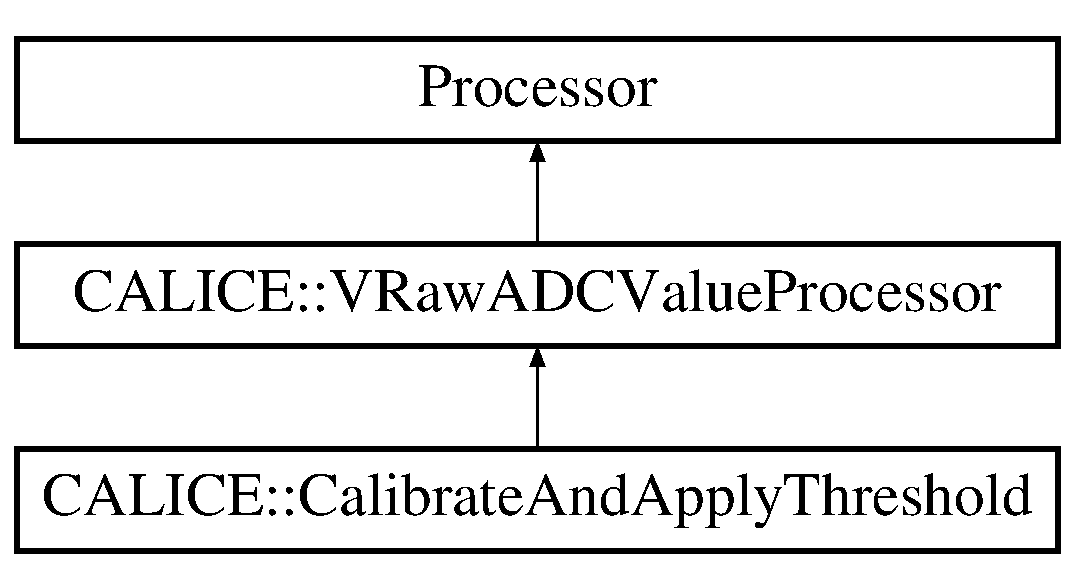
\includegraphics[height=3.000000cm]{classCALICE_1_1CalibrateAndApplyThreshold}
\end{center}
\end{figure}
\subsection*{Public Member Functions}
\begin{DoxyCompactItemize}
\item 
Processor $\ast$ {\bf new\-Processor} ()\label{classCALICE_1_1CalibrateAndApplyThreshold_a011ca53f853d3a6bc58d1a9a541a99da}

\begin{DoxyCompactList}\small\item\em construct a new Processor (required by Marlin). \end{DoxyCompactList}\item 
{\bf Calibrate\-And\-Apply\-Threshold} ()
\begin{DoxyCompactList}\small\item\em default constructor. \end{DoxyCompactList}\item 
{\bf $\sim$\-Calibrate\-And\-Apply\-Threshold} ()\label{classCALICE_1_1CalibrateAndApplyThreshold_a1318d9f3f1a695b1996c30c63c47d085}

\begin{DoxyCompactList}\small\item\em destructor. \end{DoxyCompactList}\item 
void {\bf init} ()
\begin{DoxyCompactList}\small\item\em Called at the begin of the job before anything is read. \end{DoxyCompactList}\item 
void {\bf process\-Run\-Header} (L\-C\-Run\-Header $\ast$run)\label{classCALICE_1_1CalibrateAndApplyThreshold_a3bd3d21d979363fa105e7cea54148502}

\begin{DoxyCompactList}\small\item\em Called for every run (does nothing.) \end{DoxyCompactList}\item 
void {\bf process\-Event} (L\-C\-Event $\ast$evt\-P)
\begin{DoxyCompactList}\small\item\em Reconstruct calorimeter hits. \end{DoxyCompactList}\item 
void {\bfseries end} ()\label{classCALICE_1_1CalibrateAndApplyThreshold_a9779b4e112b4cae16dec00d158f656f2}

\end{DoxyCompactItemize}
\subsection*{Private Member Functions}
\begin{DoxyCompactItemize}
\item 
void {\bfseries detector\-Transformation\-Changed} (lcio\-::\-L\-C\-Collection $\ast$col)\label{classCALICE_1_1CalibrateAndApplyThreshold_a160acdea77969ab85d10dfbf4ba6b719}

\item 
void {\bfseries reference\-Transformation\-Changed} (lcio\-::\-L\-C\-Collection $\ast$col)\label{classCALICE_1_1CalibrateAndApplyThreshold_aca4443deb520f3c16061d3d2364ccf16}

\end{DoxyCompactItemize}
\subsection*{Private Attributes}
\begin{DoxyCompactItemize}
\item 
{\bf Calibration} $\ast$ {\bfseries \-\_\-calibration}\label{classCALICE_1_1CalibrateAndApplyThreshold_a5f7e659b256a90f073328936dfca032d}

\item 
L\-C\-Collection $\ast$ {\bfseries \-\_\-cell\-Col}\label{classCALICE_1_1CalibrateAndApplyThreshold_a1379ee3029e35c09bcf02a555f79bce2}

\item 
std\-::string {\bfseries \-\_\-cell\-Parameter\-Collection\-Name}\label{classCALICE_1_1CalibrateAndApplyThreshold_aaee3b361269a3d245228c6a7b0866f0e}

\item 
Int\-Vec {\bfseries \-\_\-adc\-Range}\label{classCALICE_1_1CalibrateAndApplyThreshold_a930eaf481f0ed35420ee5a4c87e50bc5}

\item 
Float\-\_\-t {\bf \-\_\-signal\-Threshold}
\begin{DoxyCompactList}\small\item\em Signals above the signal threshold and ... \end{DoxyCompactList}\item 
Float\-Vec {\bf \-\_\-noise\-Cut\-Vec}
\begin{DoxyCompactList}\small\item\em above the noise cut are considered to be hits. \end{DoxyCompactList}\item 
Float\-\_\-t {\bf \-\_\-noise\-Cut}\label{classCALICE_1_1CalibrateAndApplyThreshold_a457ab672e3467ed409a58e42e4aa6229}

\begin{DoxyCompactList}\small\item\em will be set by the first element of the \-\_\-noise\-Cut\-Vec \end{DoxyCompactList}\item 
std\-::string {\bf \-\_\-rawhit\-Col\-Name}
\begin{DoxyCompactList}\small\item\em Name of the hit collection (I\-N\-P\-U\-T). \end{DoxyCompactList}\item 
std\-::string {\bf \-\_\-hit\-Col\-Name}
\begin{DoxyCompactList}\small\item\em Name of the hit collection (O\-U\-T\-P\-U\-T). \end{DoxyCompactList}\item 
bool {\bf \-\_\-link\-Rec\-To\-Sim}\label{classCALICE_1_1CalibrateAndApplyThreshold_aba8a11b61c43b9339e3140839fc5b213}

\begin{DoxyCompactList}\small\item\em kkk flag to disable/enable the creation of an L\-C\-Relation to simulated hit \end{DoxyCompactList}\item 
std\-::string {\bf \-\_\-\-Rec\-To\-Sim\-Col\-Name}
\begin{DoxyCompactList}\small\item\em kkk\-: Name of the relation collection hit -\/$>$ simhit (O\-U\-T\-P\-U\-T). \end{DoxyCompactList}\item 
std\-::string {\bf \-\_\-\-Raw\-To\-Sim\-Col\-Name}
\begin{DoxyCompactList}\small\item\em Name of the relation collection between Sim and Raw hits (I\-N\-P\-U\-T). \end{DoxyCompactList}\item 
std\-::string {\bf \-\_\-calibration\-Object\-Name}\label{classCALICE_1_1CalibrateAndApplyThreshold_a36efa661235242659c74a49235164662}

\begin{DoxyCompactList}\small\item\em Name of the \doxyref{Calibration}{p.}{classCalibration} object to be used (will be created using the \doxyref{Calibration\-Factory}{p.}{classCalibrationFactory}) \end{DoxyCompactList}\item 
std\-::string {\bf \-\_\-calibration\-Constant\-Col\-Name}
\begin{DoxyCompactList}\small\item\em Name of the conditions data collection containing the calibration constants. \end{DoxyCompactList}\item 
Bool\-\_\-t {\bfseries \-\_\-calibration\-On}\label{classCALICE_1_1CalibrateAndApplyThreshold_a1381fda668d89ec76ac565580e7fca36}

\item 
U\-Int\-\_\-t {\bfseries \-\_\-last\-Event}\label{classCALICE_1_1CalibrateAndApplyThreshold_ab2f19b2717ad2afc75043a35478f3ceb}

\item 
U\-Int\-\_\-t {\bfseries \-\_\-n\-Events\-Without\-R\-A\-W\-H\-I\-T\-S}\label{classCALICE_1_1CalibrateAndApplyThreshold_acf199915d32e1c4cb6d9a87f4a0373ff}

\item 
U\-Int\-\_\-t {\bfseries \-\_\-n\-Events\-Without\-S\-I\-M\-H\-I\-T\-S}\label{classCALICE_1_1CalibrateAndApplyThreshold_ae3e308ce27f5c1dd19bfee64a4d68892}

\item 
U\-Int\-\_\-t {\bfseries \-\_\-n\-Evt}\label{classCALICE_1_1CalibrateAndApplyThreshold_a80c7d9d42453384e5f8b12eee3e6b377}

\item 
Int\-\_\-t {\bfseries \-\_\-save\-Histograms}\label{classCALICE_1_1CalibrateAndApplyThreshold_a05f90325598b42ff4e8b0af45cedc99b}

\item 
Run\-Information {\bfseries \-\_\-run\-Info}\label{classCALICE_1_1CalibrateAndApplyThreshold_afa4a2e593f7eabd44817705637f2f5b8}

\item 
T\-String {\bfseries \-\_\-rootname}\label{classCALICE_1_1CalibrateAndApplyThreshold_ad54aa68d7f9f558d3556c1e387043e0b}

\item 
T\-File $\ast$ {\bfseries \-\_\-hfile}\label{classCALICE_1_1CalibrateAndApplyThreshold_adfab3548f6b0c6e4cce5436cc679bfb6}

\item 
T\-H1\-F $\ast$ {\bfseries p\-\_\-noise} [30][324]\label{classCALICE_1_1CalibrateAndApplyThreshold_a2a1569bd1101d3c46b178524e2280953}

\item 
T\-H1\-F $\ast$ {\bfseries p\-\_\-raw\-Ampl} [30][324]\label{classCALICE_1_1CalibrateAndApplyThreshold_a0773507c8f06882bb5c7b62fd4ac533b}

\item 
T\-H1\-F $\ast$ {\bfseries p\-\_\-ped\-Corr} [30][324]\label{classCALICE_1_1CalibrateAndApplyThreshold_ae1a721c77f3bf49fffff7ec31fddb214}

\item 
T\-H1\-F $\ast$ {\bfseries p\-\_\-cal\-Val} [30][324]\label{classCALICE_1_1CalibrateAndApplyThreshold_ae443cba04fd5819e9a42cd514fb9ca50}

\item 
T\-H1\-F $\ast$ {\bfseries p\-\_\-sig} [30][324]\label{classCALICE_1_1CalibrateAndApplyThreshold_a479cc39be89fcaa154f96571e63843d4}

\item 
T\-H1\-F $\ast$ {\bfseries p\-\_\-\-So\-N} [30][324]\label{classCALICE_1_1CalibrateAndApplyThreshold_a8d5fb256bddd8b8aad93138bbf50c1d7}

\item 
std\-::string {\bf \-\_\-col\-Name\-Detector\-Transformation}
\begin{DoxyCompactList}\small\item\em Name of the conditions data collection which describes the position and the rotation of the detector. \end{DoxyCompactList}\item 
std\-::string {\bf \-\_\-col\-Name\-Reference\-Transformation}
\begin{DoxyCompactList}\small\item\em Name of the conditions data collection which describes the reference position and rotation. \end{DoxyCompactList}\item 
Conditions\-Change\-Delegator\\*
$<$ {\bf Calibrate\-And\-Apply\-Threshold} $>$ {\bf \-\_\-detector\-Transformation\-Change}
\begin{DoxyCompactList}\small\item\em helper class to listen for changes of the detector position or rotation. \end{DoxyCompactList}\item 
Conditions\-Change\-Delegator\\*
$<$ {\bf Calibrate\-And\-Apply\-Threshold} $>$ {\bf \-\_\-reference\-Transformation\-Change}
\begin{DoxyCompactList}\small\item\em helper class to listen for changes of the reference position or rotation. \end{DoxyCompactList}\item 
float {\bfseries \-\_\-fallback\-Shift}\label{classCALICE_1_1CalibrateAndApplyThreshold_a23959025f1e0fb5c0a177cd6ebbaa217}

\end{DoxyCompactItemize}
\subsection*{Additional Inherited Members}


\subsection{Detailed Description}
Marlin Processor to go from Raw\-Calorimeter\-Hit to calibrated Calorimeter\-Hits. 

The hit position is calculated using information stored in a the cell\-I\-D1. Moreover, the signal is calibrated if a proper calibration object exists. should run on Data as well as on M\-C after digisim. \begin{DoxyRefDesc}{Todo}
\item[{\bf Todo}](Re-\/)Verify its applicability for M\-C after modifs for this release!!!! \end{DoxyRefDesc}


Definition at line 36 of file Calibrate\-And\-Apply\-Threshold.\-hh.



\subsection{Constructor \& Destructor Documentation}
\index{C\-A\-L\-I\-C\-E\-::\-Calibrate\-And\-Apply\-Threshold@{C\-A\-L\-I\-C\-E\-::\-Calibrate\-And\-Apply\-Threshold}!Calibrate\-And\-Apply\-Threshold@{Calibrate\-And\-Apply\-Threshold}}
\index{Calibrate\-And\-Apply\-Threshold@{Calibrate\-And\-Apply\-Threshold}!CALICE::CalibrateAndApplyThreshold@{C\-A\-L\-I\-C\-E\-::\-Calibrate\-And\-Apply\-Threshold}}
\subsubsection[{Calibrate\-And\-Apply\-Threshold}]{\setlength{\rightskip}{0pt plus 5cm}C\-A\-L\-I\-C\-E\-::\-Calibrate\-And\-Apply\-Threshold\-::\-Calibrate\-And\-Apply\-Threshold (
\begin{DoxyParamCaption}
{}
\end{DoxyParamCaption}
)}\label{classCALICE_1_1CalibrateAndApplyThreshold_ae2d615ca7797434d642f1ae6d6950974}


default constructor. 

defines and registers its parameters. 

Definition at line 46 of file Calibrate\-And\-Apply\-Threshold.\-cc.



References \-\_\-calibration\-Constant\-Col\-Name, \-\_\-calibration\-Object\-Name, \-\_\-col\-Name\-Detector\-Transformation, \-\_\-col\-Name\-Reference\-Transformation, \-\_\-hit\-Col\-Name, \-\_\-link\-Rec\-To\-Sim, \-\_\-noise\-Cut\-Vec, \-\_\-rawhit\-Col\-Name, \-\_\-\-Raw\-To\-Sim\-Col\-Name, \-\_\-\-Rec\-To\-Sim\-Col\-Name, and \-\_\-signal\-Threshold.



Referenced by new\-Processor().



\subsection{Member Function Documentation}
\index{C\-A\-L\-I\-C\-E\-::\-Calibrate\-And\-Apply\-Threshold@{C\-A\-L\-I\-C\-E\-::\-Calibrate\-And\-Apply\-Threshold}!init@{init}}
\index{init@{init}!CALICE::CalibrateAndApplyThreshold@{C\-A\-L\-I\-C\-E\-::\-Calibrate\-And\-Apply\-Threshold}}
\subsubsection[{init}]{\setlength{\rightskip}{0pt plus 5cm}void C\-A\-L\-I\-C\-E\-::\-Calibrate\-And\-Apply\-Threshold\-::init (
\begin{DoxyParamCaption}
{}
\end{DoxyParamCaption}
)}\label{classCALICE_1_1CalibrateAndApplyThreshold_a69d43c0be2a238e99828c918003bde74}


Called at the begin of the job before anything is read. 

Use to initialize the processor, e.\-g. book histograms. 

Definition at line 142 of file Calibrate\-And\-Apply\-Threshold.\-cc.



References \-\_\-calibration\-Constant\-Col\-Name, \-\_\-calibration\-Object\-Name, \-\_\-col\-Name\-Detector\-Transformation, C\-A\-L\-I\-C\-E\-::\-V\-Raw\-A\-D\-C\-Value\-Processor\-::\-\_\-col\-Name\-Module\-Description, \-\_\-col\-Name\-Reference\-Transformation, \-\_\-detector\-Transformation\-Change, \-\_\-noise\-Cut, \-\_\-noise\-Cut\-Vec, \-\_\-reference\-Transformation\-Change, Calibration\-Factory\-::create\-Calibration\-Object(), Calibration\-Factory\-::get\-Instance(), and Calibration\-Factory\-::list\-Kits().

\index{C\-A\-L\-I\-C\-E\-::\-Calibrate\-And\-Apply\-Threshold@{C\-A\-L\-I\-C\-E\-::\-Calibrate\-And\-Apply\-Threshold}!process\-Event@{process\-Event}}
\index{process\-Event@{process\-Event}!CALICE::CalibrateAndApplyThreshold@{C\-A\-L\-I\-C\-E\-::\-Calibrate\-And\-Apply\-Threshold}}
\subsubsection[{process\-Event}]{\setlength{\rightskip}{0pt plus 5cm}void C\-A\-L\-I\-C\-E\-::\-Calibrate\-And\-Apply\-Threshold\-::process\-Event (
\begin{DoxyParamCaption}
\item[{L\-C\-Event $\ast$}]{evt\-P}
\end{DoxyParamCaption}
)}\label{classCALICE_1_1CalibrateAndApplyThreshold_a2c3e34db11fe08fab2b184cc87f4d7b5}


Reconstruct calorimeter hits. 

The class needs as input the Raw\-Calorimeter\-Hit collection from \doxyref{Simple\-Hit\-Search}{p.}{classCALICE_1_1SimpleHitSearch} or digisim and produces a Calorimeter\-Hit collection. 

Definition at line 247 of file Calibrate\-And\-Apply\-Threshold.\-cc.



References \-\_\-hit\-Col\-Name, \-\_\-link\-Rec\-To\-Sim, \-\_\-noise\-Cut, \-\_\-rawhit\-Col\-Name, \-\_\-\-Raw\-To\-Sim\-Col\-Name, \-\_\-\-Rec\-To\-Sim\-Col\-Name, \-\_\-signal\-Threshold, Calibration\-::get\-Calibrated\-Value(), Calibration\-::get\-Minium\-A\-D\-C\-For\-Mip\-Threshold(), C\-A\-L\-I\-C\-E\-::\-Noise\-Parameter\-::get\-Noise(), and C\-A\-L\-I\-C\-E\-::\-Noise\-Parameter\-::is\-Dead().



\subsection{Field Documentation}
\index{C\-A\-L\-I\-C\-E\-::\-Calibrate\-And\-Apply\-Threshold@{C\-A\-L\-I\-C\-E\-::\-Calibrate\-And\-Apply\-Threshold}!\-\_\-calibration\-Constant\-Col\-Name@{\-\_\-calibration\-Constant\-Col\-Name}}
\index{\-\_\-calibration\-Constant\-Col\-Name@{\-\_\-calibration\-Constant\-Col\-Name}!CALICE::CalibrateAndApplyThreshold@{C\-A\-L\-I\-C\-E\-::\-Calibrate\-And\-Apply\-Threshold}}
\subsubsection[{\-\_\-calibration\-Constant\-Col\-Name}]{\setlength{\rightskip}{0pt plus 5cm}std\-::string C\-A\-L\-I\-C\-E\-::\-Calibrate\-And\-Apply\-Threshold\-::\-\_\-calibration\-Constant\-Col\-Name\hspace{0.3cm}{\ttfamily [private]}}\label{classCALICE_1_1CalibrateAndApplyThreshold_a79e5cf6fc879e14cdd3c68f88b1ff7c1}


Name of the conditions data collection containing the calibration constants. 



Definition at line 100 of file Calibrate\-And\-Apply\-Threshold.\-hh.



Referenced by Calibrate\-And\-Apply\-Threshold(), and init().

\index{C\-A\-L\-I\-C\-E\-::\-Calibrate\-And\-Apply\-Threshold@{C\-A\-L\-I\-C\-E\-::\-Calibrate\-And\-Apply\-Threshold}!\-\_\-col\-Name\-Detector\-Transformation@{\-\_\-col\-Name\-Detector\-Transformation}}
\index{\-\_\-col\-Name\-Detector\-Transformation@{\-\_\-col\-Name\-Detector\-Transformation}!CALICE::CalibrateAndApplyThreshold@{C\-A\-L\-I\-C\-E\-::\-Calibrate\-And\-Apply\-Threshold}}
\subsubsection[{\-\_\-col\-Name\-Detector\-Transformation}]{\setlength{\rightskip}{0pt plus 5cm}std\-::string C\-A\-L\-I\-C\-E\-::\-Calibrate\-And\-Apply\-Threshold\-::\-\_\-col\-Name\-Detector\-Transformation\hspace{0.3cm}{\ttfamily [private]}}\label{classCALICE_1_1CalibrateAndApplyThreshold_a4a6e48e29b530ac9b80375776cd4af31}


Name of the conditions data collection which describes the position and the rotation of the detector. 



Definition at line 124 of file Calibrate\-And\-Apply\-Threshold.\-hh.



Referenced by Calibrate\-And\-Apply\-Threshold(), and init().

\index{C\-A\-L\-I\-C\-E\-::\-Calibrate\-And\-Apply\-Threshold@{C\-A\-L\-I\-C\-E\-::\-Calibrate\-And\-Apply\-Threshold}!\-\_\-col\-Name\-Reference\-Transformation@{\-\_\-col\-Name\-Reference\-Transformation}}
\index{\-\_\-col\-Name\-Reference\-Transformation@{\-\_\-col\-Name\-Reference\-Transformation}!CALICE::CalibrateAndApplyThreshold@{C\-A\-L\-I\-C\-E\-::\-Calibrate\-And\-Apply\-Threshold}}
\subsubsection[{\-\_\-col\-Name\-Reference\-Transformation}]{\setlength{\rightskip}{0pt plus 5cm}std\-::string C\-A\-L\-I\-C\-E\-::\-Calibrate\-And\-Apply\-Threshold\-::\-\_\-col\-Name\-Reference\-Transformation\hspace{0.3cm}{\ttfamily [private]}}\label{classCALICE_1_1CalibrateAndApplyThreshold_a3e6c0435de64d50ae08374cf145c8c8b}


Name of the conditions data collection which describes the reference position and rotation. 



Definition at line 126 of file Calibrate\-And\-Apply\-Threshold.\-hh.



Referenced by Calibrate\-And\-Apply\-Threshold(), and init().

\index{C\-A\-L\-I\-C\-E\-::\-Calibrate\-And\-Apply\-Threshold@{C\-A\-L\-I\-C\-E\-::\-Calibrate\-And\-Apply\-Threshold}!\-\_\-detector\-Transformation\-Change@{\-\_\-detector\-Transformation\-Change}}
\index{\-\_\-detector\-Transformation\-Change@{\-\_\-detector\-Transformation\-Change}!CALICE::CalibrateAndApplyThreshold@{C\-A\-L\-I\-C\-E\-::\-Calibrate\-And\-Apply\-Threshold}}
\subsubsection[{\-\_\-detector\-Transformation\-Change}]{\setlength{\rightskip}{0pt plus 5cm}Conditions\-Change\-Delegator$<${\bf Calibrate\-And\-Apply\-Threshold}$>$ C\-A\-L\-I\-C\-E\-::\-Calibrate\-And\-Apply\-Threshold\-::\-\_\-detector\-Transformation\-Change\hspace{0.3cm}{\ttfamily [private]}}\label{classCALICE_1_1CalibrateAndApplyThreshold_a9f46c5087b5975ec06c36e9da4f33378}


helper class to listen for changes of the detector position or rotation. 



Definition at line 130 of file Calibrate\-And\-Apply\-Threshold.\-hh.



Referenced by init().

\index{C\-A\-L\-I\-C\-E\-::\-Calibrate\-And\-Apply\-Threshold@{C\-A\-L\-I\-C\-E\-::\-Calibrate\-And\-Apply\-Threshold}!\-\_\-hit\-Col\-Name@{\-\_\-hit\-Col\-Name}}
\index{\-\_\-hit\-Col\-Name@{\-\_\-hit\-Col\-Name}!CALICE::CalibrateAndApplyThreshold@{C\-A\-L\-I\-C\-E\-::\-Calibrate\-And\-Apply\-Threshold}}
\subsubsection[{\-\_\-hit\-Col\-Name}]{\setlength{\rightskip}{0pt plus 5cm}std\-::string C\-A\-L\-I\-C\-E\-::\-Calibrate\-And\-Apply\-Threshold\-::\-\_\-hit\-Col\-Name\hspace{0.3cm}{\ttfamily [private]}}\label{classCALICE_1_1CalibrateAndApplyThreshold_a10dd53b4f7d1514791ec6c60329aaea4}


Name of the hit collection (O\-U\-T\-P\-U\-T). 



Definition at line 93 of file Calibrate\-And\-Apply\-Threshold.\-hh.



Referenced by Calibrate\-And\-Apply\-Threshold(), and process\-Event().

\index{C\-A\-L\-I\-C\-E\-::\-Calibrate\-And\-Apply\-Threshold@{C\-A\-L\-I\-C\-E\-::\-Calibrate\-And\-Apply\-Threshold}!\-\_\-noise\-Cut\-Vec@{\-\_\-noise\-Cut\-Vec}}
\index{\-\_\-noise\-Cut\-Vec@{\-\_\-noise\-Cut\-Vec}!CALICE::CalibrateAndApplyThreshold@{C\-A\-L\-I\-C\-E\-::\-Calibrate\-And\-Apply\-Threshold}}
\subsubsection[{\-\_\-noise\-Cut\-Vec}]{\setlength{\rightskip}{0pt plus 5cm}Float\-Vec C\-A\-L\-I\-C\-E\-::\-Calibrate\-And\-Apply\-Threshold\-::\-\_\-noise\-Cut\-Vec\hspace{0.3cm}{\ttfamily [private]}}\label{classCALICE_1_1CalibrateAndApplyThreshold_adfacf11438d8b5f863f6e77722dc5e20}


above the noise cut are considered to be hits. 

This vector contains a cut for the hit search and for the hit rejection during noise calculation 

Definition at line 87 of file Calibrate\-And\-Apply\-Threshold.\-hh.



Referenced by Calibrate\-And\-Apply\-Threshold(), and init().

\index{C\-A\-L\-I\-C\-E\-::\-Calibrate\-And\-Apply\-Threshold@{C\-A\-L\-I\-C\-E\-::\-Calibrate\-And\-Apply\-Threshold}!\-\_\-rawhit\-Col\-Name@{\-\_\-rawhit\-Col\-Name}}
\index{\-\_\-rawhit\-Col\-Name@{\-\_\-rawhit\-Col\-Name}!CALICE::CalibrateAndApplyThreshold@{C\-A\-L\-I\-C\-E\-::\-Calibrate\-And\-Apply\-Threshold}}
\subsubsection[{\-\_\-rawhit\-Col\-Name}]{\setlength{\rightskip}{0pt plus 5cm}std\-::string C\-A\-L\-I\-C\-E\-::\-Calibrate\-And\-Apply\-Threshold\-::\-\_\-rawhit\-Col\-Name\hspace{0.3cm}{\ttfamily [private]}}\label{classCALICE_1_1CalibrateAndApplyThreshold_a3a6f0a6d75fa972ac6303604bb515fc7}


Name of the hit collection (I\-N\-P\-U\-T). 



Definition at line 92 of file Calibrate\-And\-Apply\-Threshold.\-hh.



Referenced by Calibrate\-And\-Apply\-Threshold(), and process\-Event().

\index{C\-A\-L\-I\-C\-E\-::\-Calibrate\-And\-Apply\-Threshold@{C\-A\-L\-I\-C\-E\-::\-Calibrate\-And\-Apply\-Threshold}!\-\_\-\-Raw\-To\-Sim\-Col\-Name@{\-\_\-\-Raw\-To\-Sim\-Col\-Name}}
\index{\-\_\-\-Raw\-To\-Sim\-Col\-Name@{\-\_\-\-Raw\-To\-Sim\-Col\-Name}!CALICE::CalibrateAndApplyThreshold@{C\-A\-L\-I\-C\-E\-::\-Calibrate\-And\-Apply\-Threshold}}
\subsubsection[{\-\_\-\-Raw\-To\-Sim\-Col\-Name}]{\setlength{\rightskip}{0pt plus 5cm}std\-::string C\-A\-L\-I\-C\-E\-::\-Calibrate\-And\-Apply\-Threshold\-::\-\_\-\-Raw\-To\-Sim\-Col\-Name\hspace{0.3cm}{\ttfamily [private]}}\label{classCALICE_1_1CalibrateAndApplyThreshold_a75f2b80baf0f8691c9d921d70bafb649}


Name of the relation collection between Sim and Raw hits (I\-N\-P\-U\-T). 



Definition at line 97 of file Calibrate\-And\-Apply\-Threshold.\-hh.



Referenced by Calibrate\-And\-Apply\-Threshold(), and process\-Event().

\index{C\-A\-L\-I\-C\-E\-::\-Calibrate\-And\-Apply\-Threshold@{C\-A\-L\-I\-C\-E\-::\-Calibrate\-And\-Apply\-Threshold}!\-\_\-\-Rec\-To\-Sim\-Col\-Name@{\-\_\-\-Rec\-To\-Sim\-Col\-Name}}
\index{\-\_\-\-Rec\-To\-Sim\-Col\-Name@{\-\_\-\-Rec\-To\-Sim\-Col\-Name}!CALICE::CalibrateAndApplyThreshold@{C\-A\-L\-I\-C\-E\-::\-Calibrate\-And\-Apply\-Threshold}}
\subsubsection[{\-\_\-\-Rec\-To\-Sim\-Col\-Name}]{\setlength{\rightskip}{0pt plus 5cm}std\-::string C\-A\-L\-I\-C\-E\-::\-Calibrate\-And\-Apply\-Threshold\-::\-\_\-\-Rec\-To\-Sim\-Col\-Name\hspace{0.3cm}{\ttfamily [private]}}\label{classCALICE_1_1CalibrateAndApplyThreshold_a6ba0e8c707c10c6ace7b034293d34035}


kkk\-: Name of the relation collection hit -\/$>$ simhit (O\-U\-T\-P\-U\-T). 



Definition at line 96 of file Calibrate\-And\-Apply\-Threshold.\-hh.



Referenced by Calibrate\-And\-Apply\-Threshold(), and process\-Event().

\index{C\-A\-L\-I\-C\-E\-::\-Calibrate\-And\-Apply\-Threshold@{C\-A\-L\-I\-C\-E\-::\-Calibrate\-And\-Apply\-Threshold}!\-\_\-reference\-Transformation\-Change@{\-\_\-reference\-Transformation\-Change}}
\index{\-\_\-reference\-Transformation\-Change@{\-\_\-reference\-Transformation\-Change}!CALICE::CalibrateAndApplyThreshold@{C\-A\-L\-I\-C\-E\-::\-Calibrate\-And\-Apply\-Threshold}}
\subsubsection[{\-\_\-reference\-Transformation\-Change}]{\setlength{\rightskip}{0pt plus 5cm}Conditions\-Change\-Delegator$<${\bf Calibrate\-And\-Apply\-Threshold}$>$ C\-A\-L\-I\-C\-E\-::\-Calibrate\-And\-Apply\-Threshold\-::\-\_\-reference\-Transformation\-Change\hspace{0.3cm}{\ttfamily [private]}}\label{classCALICE_1_1CalibrateAndApplyThreshold_a1e6bdda0ecedd7a21053f54f178478b1}


helper class to listen for changes of the reference position or rotation. 



Definition at line 133 of file Calibrate\-And\-Apply\-Threshold.\-hh.



Referenced by init().

\index{C\-A\-L\-I\-C\-E\-::\-Calibrate\-And\-Apply\-Threshold@{C\-A\-L\-I\-C\-E\-::\-Calibrate\-And\-Apply\-Threshold}!\-\_\-signal\-Threshold@{\-\_\-signal\-Threshold}}
\index{\-\_\-signal\-Threshold@{\-\_\-signal\-Threshold}!CALICE::CalibrateAndApplyThreshold@{C\-A\-L\-I\-C\-E\-::\-Calibrate\-And\-Apply\-Threshold}}
\subsubsection[{\-\_\-signal\-Threshold}]{\setlength{\rightskip}{0pt plus 5cm}Float\-\_\-t C\-A\-L\-I\-C\-E\-::\-Calibrate\-And\-Apply\-Threshold\-::\-\_\-signal\-Threshold\hspace{0.3cm}{\ttfamily [private]}}\label{classCALICE_1_1CalibrateAndApplyThreshold_a7c318b024c59652ac1989c8c1486aa49}


Signals above the signal threshold and ... 



Definition at line 86 of file Calibrate\-And\-Apply\-Threshold.\-hh.



Referenced by Calibrate\-And\-Apply\-Threshold(), and process\-Event().



The documentation for this class was generated from the following files\-:\begin{DoxyCompactItemize}
\item 
Calibrate\-And\-Apply\-Threshold.\-hh\item 
Calibrate\-And\-Apply\-Threshold.\-cc\end{DoxyCompactItemize}

\section{Calibration Class Reference}
\label{classCalibration}\index{Calibration@{Calibration}}


Abstract interface of a calibration object.  




{\ttfamily \#include $<$Calibration.\-hh$>$}

Inheritance diagram for Calibration\-:\begin{figure}[H]
\begin{center}
\leavevmode
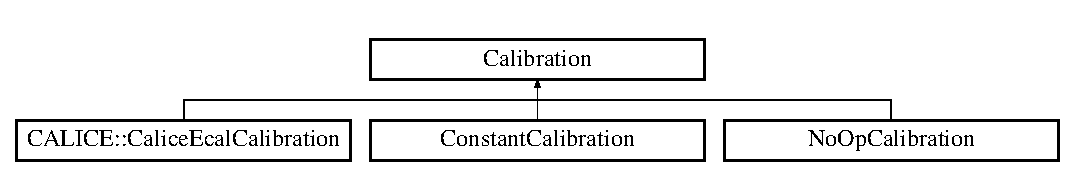
\includegraphics[height=1.934370cm]{classCalibration}
\end{center}
\end{figure}
\subsection*{Public Member Functions}
\begin{DoxyCompactItemize}
\item 
virtual Float\-\_\-t {\bf get\-Calibrated\-Value} (U\-Int\-\_\-t module\-\_\-id, U\-Int\-\_\-t module\-\_\-type, U\-Int\-\_\-t cell\-\_\-index, Float\-\_\-t adc\-\_\-value) const =0
\begin{DoxyCompactList}\small\item\em Determine from a pedestal subtracted A\-D\-C value a calibrated value. \end{DoxyCompactList}\item 
virtual Bool\-\_\-t {\bf is\-Valid} (U\-Int\-\_\-t module\-\_\-id, U\-Int\-\_\-t module\-\_\-type, U\-Int\-\_\-t cell\-\_\-index) const 
\begin{DoxyCompactList}\small\item\em Return true if a the calibration constants for the given cell are in the allowed range. \end{DoxyCompactList}\item 
virtual Bool\-\_\-t {\bf check\-For\-Calibration\-Constants\-Of\-Module} (U\-Int\-\_\-t module\-\_\-id, U\-Int\-\_\-t module\-\_\-type, U\-Int\-\_\-t n\-\_\-cells) const =0
\begin{DoxyCompactList}\small\item\em Verify that calibration constants exist for a certain module. \end{DoxyCompactList}\item 
virtual Int\-\_\-t {\bf get\-Minium\-A\-D\-C\-For\-Mip\-Threshold} (Float\-\_\-t mip\-\_\-energy\-\_\-fraction) const =0
\begin{DoxyCompactList}\small\item\em Get the minimum adc value mips will have for the given energy fraction on all pads. \end{DoxyCompactList}\end{DoxyCompactItemize}


\subsection{Detailed Description}
Abstract interface of a calibration object. 

The calibration object returns for a value measured with a certain cell a calibrated value. 

Definition at line 9 of file Calibration.\-hh.



\subsection{Member Function Documentation}
\index{Calibration@{Calibration}!check\-For\-Calibration\-Constants\-Of\-Module@{check\-For\-Calibration\-Constants\-Of\-Module}}
\index{check\-For\-Calibration\-Constants\-Of\-Module@{check\-For\-Calibration\-Constants\-Of\-Module}!Calibration@{Calibration}}
\subsubsection[{check\-For\-Calibration\-Constants\-Of\-Module}]{\setlength{\rightskip}{0pt plus 5cm}virtual Bool\-\_\-t Calibration\-::check\-For\-Calibration\-Constants\-Of\-Module (
\begin{DoxyParamCaption}
\item[{U\-Int\-\_\-t}]{module\-\_\-id, }
\item[{U\-Int\-\_\-t}]{module\-\_\-type, }
\item[{U\-Int\-\_\-t}]{n\-\_\-cells}
\end{DoxyParamCaption}
) const\hspace{0.3cm}{\ttfamily [pure virtual]}}\label{classCalibration_a04c8f21c6e77cd3c91c858ca2c9373c4}


Verify that calibration constants exist for a certain module. 


\begin{DoxyParams}{Parameters}
{\em module\-\_\-id} & id Or serial number of a module which uniquely identifies a detector module of a certain type. \\
\hline
{\em module\-\_\-type} & the type of the detector module \\
\hline
{\em n\-\_\-cells} & the number of cells on this module. Return true if calibration constants exist for the given module and the number of cells matches the number of calibration constants. \\
\hline
\end{DoxyParams}


Implemented in {\bf Constant\-Calibration} \doxyref{}{p.}{classConstantCalibration_aec30f5342ec651fa61708d2675e14d05}, and {\bf No\-Op\-Calibration} \doxyref{}{p.}{classNoOpCalibration_acdb31ec76cef7720c0cda5fb15ffa2fb}.



Referenced by C\-A\-L\-I\-C\-E\-::\-Simple\-Hit\-Search\-::build\-Cell\-Parameters().

\index{Calibration@{Calibration}!get\-Calibrated\-Value@{get\-Calibrated\-Value}}
\index{get\-Calibrated\-Value@{get\-Calibrated\-Value}!Calibration@{Calibration}}
\subsubsection[{get\-Calibrated\-Value}]{\setlength{\rightskip}{0pt plus 5cm}virtual Float\-\_\-t Calibration\-::get\-Calibrated\-Value (
\begin{DoxyParamCaption}
\item[{U\-Int\-\_\-t}]{module\-\_\-id, }
\item[{U\-Int\-\_\-t}]{module\-\_\-type, }
\item[{U\-Int\-\_\-t}]{cell\-\_\-index, }
\item[{Float\-\_\-t}]{adc\-\_\-value}
\end{DoxyParamCaption}
) const\hspace{0.3cm}{\ttfamily [pure virtual]}}\label{classCalibration_aca88d93a445ba3021c05dd61b293568c}


Determine from a pedestal subtracted A\-D\-C value a calibrated value. 


\begin{DoxyParams}{Parameters}
{\em module\-\_\-id} & id Or serial number of a module which uniquely identifies a detector module of a certain type. \\
\hline
{\em module\-\_\-type} & the type of the detector module \\
\hline
{\em cell\-\_\-index} & the cell\-\_\-index in read order\-: first the A\-D\-C values of the first sample from all chips, then the next sample ... \\
\hline
{\em adc\-\_\-value} & the A\-D\-C value which should be calibrated. \\
\hline
\end{DoxyParams}
\begin{DoxyReturn}{Returns}
the calibrated value. 
\end{DoxyReturn}


Implemented in {\bf Constant\-Calibration} \doxyref{}{p.}{classConstantCalibration_a347808435c2c9e499af4c9a83d1c6915}, and {\bf No\-Op\-Calibration} \doxyref{}{p.}{classNoOpCalibration_a8dd43819c4e5bb09e097f4db360a57fe}.



Referenced by C\-A\-L\-I\-C\-E\-::\-Calibrate\-And\-Apply\-Threshold\-::process\-Event().

\index{Calibration@{Calibration}!get\-Minium\-A\-D\-C\-For\-Mip\-Threshold@{get\-Minium\-A\-D\-C\-For\-Mip\-Threshold}}
\index{get\-Minium\-A\-D\-C\-For\-Mip\-Threshold@{get\-Minium\-A\-D\-C\-For\-Mip\-Threshold}!Calibration@{Calibration}}
\subsubsection[{get\-Minium\-A\-D\-C\-For\-Mip\-Threshold}]{\setlength{\rightskip}{0pt plus 5cm}virtual Int\-\_\-t Calibration\-::get\-Minium\-A\-D\-C\-For\-Mip\-Threshold (
\begin{DoxyParamCaption}
\item[{Float\-\_\-t}]{mip\-\_\-energy\-\_\-fraction}
\end{DoxyParamCaption}
) const\hspace{0.3cm}{\ttfamily [pure virtual]}}\label{classCalibration_a4e45f1eca0d4fdf19ad76b8f581aee12}


Get the minimum adc value mips will have for the given energy fraction on all pads. 


\begin{DoxyParams}{Parameters}
{\em mip\-\_\-energy\-\_\-fraction} & the energy in mips \\
\hline
\end{DoxyParams}
\begin{DoxyReturn}{Returns}
minimum adc value which is below the given energy on all pads. This method can be used to get the lowest adc value a mip of the given energy fraction will have on all pads. This value is useful to select candidates before actually performing th calibration. This function is intended to be called at the beginning of each event. 
\end{DoxyReturn}


Implemented in {\bf Constant\-Calibration} \doxyref{}{p.}{classConstantCalibration_ada035fed7a513d3da391bdea2c1d23f7}, and {\bf No\-Op\-Calibration} \doxyref{}{p.}{classNoOpCalibration_a8b478c6680b5980c2b87cedc8a589989}.



Referenced by C\-A\-L\-I\-C\-E\-::\-Calibrate\-And\-Apply\-Threshold\-::process\-Event(), C\-A\-L\-I\-C\-E\-::\-Simple\-Hit\-Search\-::search\-Hits(), and C\-A\-L\-I\-C\-E\-::\-Simple\-Hit\-Search\-::search\-Hits\-And\-Adjust\-Pedestals\-And\-Noise().

\index{Calibration@{Calibration}!is\-Valid@{is\-Valid}}
\index{is\-Valid@{is\-Valid}!Calibration@{Calibration}}
\subsubsection[{is\-Valid}]{\setlength{\rightskip}{0pt plus 5cm}virtual Bool\-\_\-t Calibration\-::is\-Valid (
\begin{DoxyParamCaption}
\item[{U\-Int\-\_\-t}]{module\-\_\-id, }
\item[{U\-Int\-\_\-t}]{module\-\_\-type, }
\item[{U\-Int\-\_\-t}]{cell\-\_\-index}
\end{DoxyParamCaption}
) const\hspace{0.3cm}{\ttfamily [inline]}, {\ttfamily [virtual]}}\label{classCalibration_a7d516d7b66b1f20640829d12adfd64d6}


Return true if a the calibration constants for the given cell are in the allowed range. 


\begin{DoxyParams}{Parameters}
{\em module\-\_\-id} & id Or serial number of a module which uniquely identifies a detector module of a certain type. \\
\hline
{\em module\-\_\-type} & the type of the detector module \\
\hline
{\em cell\-\_\-index} & the cell\-\_\-index in read order\-: first the A\-D\-C values of the first sample from all chips, then the next sample ... \\
\hline
\end{DoxyParams}
\begin{DoxyReturn}{Returns}
true for cells with valid calibration constants, false for cells which should be declared dead.
\end{DoxyReturn}
This method is used to find, after module connection changes, cells which should be declared dead. 

Definition at line 31 of file Calibration.\-hh.



Referenced by C\-A\-L\-I\-C\-E\-::\-Simple\-Hit\-Search\-::build\-Cell\-Parameters(), C\-A\-L\-I\-C\-E\-::\-Calibrate\-And\-Apply\-Threshold\-::process\-Run\-Header(), C\-A\-L\-I\-C\-E\-::\-Simple\-Hit\-Search\-::reset\-For\-Initial\-Pedestal\-Noise\-Calculation(), and C\-A\-L\-I\-C\-E\-::\-Simple\-Hit\-Search\-::reset\-For\-Pedestal\-Noise\-Re\-Calculation().



The documentation for this class was generated from the following file\-:\begin{DoxyCompactItemize}
\item 
Calibration.\-hh\end{DoxyCompactItemize}

\section{Calibration\-Factory Class Reference}
\label{classCalibrationFactory}\index{Calibration\-Factory@{Calibration\-Factory}}


Return a calibration object of the given name.  




{\ttfamily \#include $<$Calibration\-Factory.\-hh$>$}

\subsection*{Public Member Functions}
\begin{DoxyCompactItemize}
\item 
void {\bf register\-Calibration\-Kit} (const std\-::string \&kit\-\_\-name, {\bf Calibration\-Kit} $\ast$a\-\_\-kit)\label{classCalibrationFactory_ae3f5c6f7204526d98c753dac871e8217}

\begin{DoxyCompactList}\small\item\em Register a \doxyref{Calibration}{p.}{classCalibration} object kit. \end{DoxyCompactList}\item 
{\bf Calibration} $\ast$ {\bf create\-Calibration\-Object} (const std\-::string \&name, const std\-::string \&module\-\_\-type\-\_\-col\-\_\-name, const std\-::string \&module\-\_\-calibration\-\_\-col\-\_\-name) noexcept(false)\label{classCalibrationFactory_a1682bde6eef1a7ff023421abc8bf4534}

\begin{DoxyCompactList}\small\item\em Get an object for the calibration. \end{DoxyCompactList}\item 
void {\bf list\-Kits} ()
\begin{DoxyCompactList}\small\item\em Show all registered kits. \end{DoxyCompactList}\end{DoxyCompactItemize}
\subsection*{Static Public Member Functions}
\begin{DoxyCompactItemize}
\item 
static {\bf Calibration\-Factory} $\ast$ {\bf get\-Instance} ()\label{classCalibrationFactory_a5efb95a0d951b8da5a8bdb5832a9831d}

\begin{DoxyCompactList}\small\item\em Get the global instance of the \doxyref{Calibration}{p.}{classCalibration} Object Factory. \end{DoxyCompactList}\end{DoxyCompactItemize}
\subsection*{Private Attributes}
\begin{DoxyCompactItemize}
\item 
std\-::map$<$ std\-::string, \\*
{\bf Calibration\-Kit} $\ast$ $>$ {\bf \-\_\-kits}
\begin{DoxyCompactList}\small\item\em List of registered \doxyref{Calibration}{p.}{classCalibration} kits. \end{DoxyCompactList}\end{DoxyCompactItemize}
\subsection*{Static Private Attributes}
\begin{DoxyCompactItemize}
\item 
static {\bf Calibration\-Factory} $\ast$ {\bf \-\_\-\-\_\-instance} =0
\begin{DoxyCompactList}\small\item\em Pointer to the global \doxyref{Calibration\-Factory}{p.}{classCalibrationFactory} instance. \end{DoxyCompactList}\end{DoxyCompactItemize}


\subsection{Detailed Description}
Return a calibration object of the given name. 

\doxyref{Calibration}{p.}{classCalibration} kits are registered with a certain name. This name which is for example specified by a Marlin parameter can than be used to create the actual calibration object. 

Definition at line 16 of file Calibration\-Factory.\-hh.



\subsection{Member Function Documentation}
\index{Calibration\-Factory@{Calibration\-Factory}!list\-Kits@{list\-Kits}}
\index{list\-Kits@{list\-Kits}!CalibrationFactory@{Calibration\-Factory}}
\subsubsection[{list\-Kits}]{\setlength{\rightskip}{0pt plus 5cm}void Calibration\-Factory\-::list\-Kits (
\begin{DoxyParamCaption}
{}
\end{DoxyParamCaption}
)}\label{classCalibrationFactory_a8ec8e4dacbc4b38c7fd760b7b00857d3}


Show all registered kits. 

For debugging. 

Definition at line 6 of file Calibration\-Factory.\-cc.



References \-\_\-kits.



Referenced by C\-A\-L\-I\-C\-E\-::\-Calibrate\-And\-Apply\-Threshold\-::init(), and C\-A\-L\-I\-C\-E\-::\-Simple\-Hit\-Search\-::init().



\subsection{Field Documentation}
\index{Calibration\-Factory@{Calibration\-Factory}!\-\_\-\-\_\-instance@{\-\_\-\-\_\-instance}}
\index{\-\_\-\-\_\-instance@{\-\_\-\-\_\-instance}!CalibrationFactory@{Calibration\-Factory}}
\subsubsection[{\-\_\-\-\_\-instance}]{\setlength{\rightskip}{0pt plus 5cm}{\bf Calibration\-Factory} $\ast$ Calibration\-Factory\-::\-\_\-\-\_\-instance =0\hspace{0.3cm}{\ttfamily [static]}, {\ttfamily [private]}}\label{classCalibrationFactory_a19b2dfab32cd94981a00a8f39e9b028b}


Pointer to the global \doxyref{Calibration\-Factory}{p.}{classCalibrationFactory} instance. 



Definition at line 64 of file Calibration\-Factory.\-hh.



Referenced by get\-Instance().

\index{Calibration\-Factory@{Calibration\-Factory}!\-\_\-kits@{\-\_\-kits}}
\index{\-\_\-kits@{\-\_\-kits}!CalibrationFactory@{Calibration\-Factory}}
\subsubsection[{\-\_\-kits}]{\setlength{\rightskip}{0pt plus 5cm}std\-::map$<$std\-::string, {\bf Calibration\-Kit} $\ast$$>$ Calibration\-Factory\-::\-\_\-kits\hspace{0.3cm}{\ttfamily [private]}}\label{classCalibrationFactory_a2ff2373b183b599ef137ee6f19e1fa6e}


List of registered \doxyref{Calibration}{p.}{classCalibration} kits. 



Definition at line 63 of file Calibration\-Factory.\-hh.



Referenced by create\-Calibration\-Object(), list\-Kits(), and register\-Calibration\-Kit().



The documentation for this class was generated from the following files\-:\begin{DoxyCompactItemize}
\item 
Calibration\-Factory.\-hh\item 
Calibration\-Factory.\-cc\end{DoxyCompactItemize}

\section{Calibration\-Kit Class Reference}
\label{classCalibrationKit}\index{Calibration\-Kit@{Calibration\-Kit}}


Abstract interface of a calibration kit which can create calibration objects.  




{\ttfamily \#include $<$Calibration\-Kit.\-hh$>$}

Inheritance diagram for Calibration\-Kit\-:\begin{figure}[H]
\begin{center}
\leavevmode
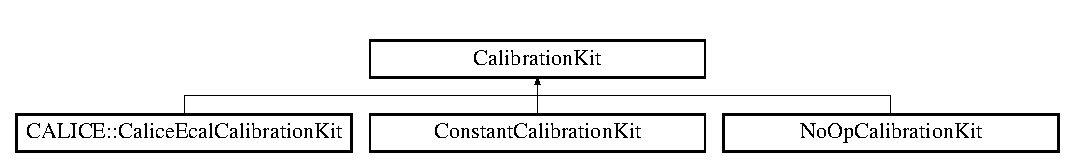
\includegraphics[height=1.803543cm]{classCalibrationKit}
\end{center}
\end{figure}
\subsection*{Public Member Functions}
\begin{DoxyCompactItemize}
\item 
virtual {\bf Calibration} $\ast$ {\bf create} (const std\-::string \&module\-\_\-type\-\_\-col\-\_\-name, const std\-::string \&module\-\_\-calibration\-\_\-col\-\_\-name) const =0
\begin{DoxyCompactList}\small\item\em create calibration object. \end{DoxyCompactList}\end{DoxyCompactItemize}


\subsection{Detailed Description}
Abstract interface of a calibration kit which can create calibration objects. 

Definition at line 11 of file Calibration\-Kit.\-hh.



\subsection{Member Function Documentation}
\index{Calibration\-Kit@{Calibration\-Kit}!create@{create}}
\index{create@{create}!CalibrationKit@{Calibration\-Kit}}
\subsubsection[{create}]{\setlength{\rightskip}{0pt plus 5cm}virtual {\bf Calibration}$\ast$ Calibration\-Kit\-::create (
\begin{DoxyParamCaption}
\item[{const std\-::string \&}]{module\-\_\-type\-\_\-col\-\_\-name, }
\item[{const std\-::string \&}]{module\-\_\-calibration\-\_\-col\-\_\-name}
\end{DoxyParamCaption}
) const\hspace{0.3cm}{\ttfamily [pure virtual]}}\label{classCalibrationKit_ab3aea5671d91a7b6f5e839324cf45a70}


create calibration object. 


\begin{DoxyParams}{Parameters}
{\em module\-\_\-type\-\_\-col\-\_\-name} & the name of the conditions data collection with the module types. \\
\hline
{\em module\-\_\-calibration\-\_\-col\-\_\-name} & the name of the conditions data collection which contains the calibration constants. F\-I\-X\-M\-E\-: There should be a better method to hand parameters to \doxyref{Calibration}{p.}{classCalibration} objects. \\
\hline
\end{DoxyParams}


Implemented in {\bf C\-A\-L\-I\-C\-E\-::\-Calice\-Ecal\-Calibration\-Kit} \doxyref{}{p.}{classCALICE_1_1CaliceEcalCalibrationKit_aa8754032807fe2e3d7d8dc4225464829}, {\bf Constant\-Calibration\-Kit} \doxyref{}{p.}{classConstantCalibrationKit_a3b84989011be10b816104fdc58963882}, and {\bf No\-Op\-Calibration\-Kit} \doxyref{}{p.}{classNoOpCalibrationKit_ac197f7bf5528b484d5b70e664655474b}.



The documentation for this class was generated from the following file\-:\begin{DoxyCompactItemize}
\item 
Calibration\-Kit.\-hh\end{DoxyCompactItemize}

\section{C\-A\-L\-I\-C\-E\-:\-:Calibration\-Set$<$ T $>$ Class Template Reference}
\label{classCALICE_1_1CalibrationSet}\index{C\-A\-L\-I\-C\-E\-::\-Calibration\-Set$<$ T $>$@{C\-A\-L\-I\-C\-E\-::\-Calibration\-Set$<$ T $>$}}


Class which handles the storage of a set of L\-C\-Hcal\-Calibration\-Object.  




{\ttfamily \#include $<$Calibration\-Set.\-hh$>$}

\subsection*{Public Types}
\begin{DoxyCompactItemize}
\item 
typedef std\-::map$<$ unsigned, T $\ast$ $>$ {\bfseries Calib\-Module\-Map}\label{classCALICE_1_1CalibrationSet_ae0ef8d231d149d1e61a4000952d58d67}

\item 
typedef std\-::pair\\*
$<$ lcio\-::\-L\-C\-Collection \\*
$\ast$, Calib\-Module\-Map $\ast$ $>$ {\bfseries Calib\-Module\-Data}\label{classCALICE_1_1CalibrationSet_a894d8c42a35b66022bb221db4585f5f5}

\item 
typedef std\-::map$<$ unsigned, \\*
Calib\-Module\-Data $>$ {\bfseries Calib\-Read\-Map}\label{classCALICE_1_1CalibrationSet_a6f4a5967aa3a3ad50d763a92809fcf60}

\end{DoxyCompactItemize}
\subsection*{Public Member Functions}
\begin{DoxyCompactItemize}
\item 
{\bfseries Calibration\-Set} ({\bf Temp\-Model} $\ast$temp\-Model)\label{classCALICE_1_1CalibrationSet_a5b3dc2a9fee4bb05ead1f6aecb63e508}

\item 
bool {\bfseries empty} ()\label{classCALICE_1_1CalibrationSet_acf72ce0c2908ad7c57c1a4fed2e0ae69}

\item 
void {\bfseries fill} (lcio\-::\-L\-C\-Collection $\ast$cal\-Col)\label{classCALICE_1_1CalibrationSet_af6eada4b282e59cd26830121ffe431ad}

\item 
void {\bfseries fill} (lcio\-::\-L\-C\-Collection $\ast$cal\-Col, lcio\-::\-L\-C\-Collection $\ast$sro\-Col)\label{classCALICE_1_1CalibrationSet_a5064acda09ac4e6f60dfd8c95575bb77}

\item 
T $\ast$ {\bfseries get\-Calib} (unsigned module\-I\-D, unsigned cell\-Key)\label{classCALICE_1_1CalibrationSet_ab7ccb1fe35ac7634ea52412ae96da4e5}

\item 
T $\ast$ {\bfseries get\-Calib} (unsigned module, unsigned chip, unsigned channel)\label{classCALICE_1_1CalibrationSet_a0e439372aeaa7d78b6fbcf0886022f1e}

\item 
void {\bfseries set\-Temp} (lcio\-::\-L\-C\-Collection $\ast$sro\-Col)\label{classCALICE_1_1CalibrationSet_a5dcbfc885e768814df5ffb3309173322}

\item 
void {\bfseries apply\-Scaling\-Factor} (float f)\label{classCALICE_1_1CalibrationSet_aba2e28745da6330c981810dd5e21f0ae}

\item 
void {\bfseries set\-Scaling\-Factor} (float f)\label{classCALICE_1_1CalibrationSet_aefc2753764d779cd34362c8a5f8b6943}

\end{DoxyCompactItemize}
\subsection*{Data Fields}
\begin{DoxyCompactItemize}
\item 
Calib\-Read\-Map {\bfseries \-\_\-read\-Map}\label{classCALICE_1_1CalibrationSet_a57c533ff2868f73cf2029d32568b3e20}

\item 
{\bf Temp\-Model} $\ast$ {\bfseries \-\_\-temp\-Model}\label{classCALICE_1_1CalibrationSet_a1076b184fc1d2ae4bb05f204fbe07f34}

\end{DoxyCompactItemize}
\subsection*{Private Attributes}
\begin{DoxyCompactItemize}
\item 
float {\bfseries \-\_\-scaling\-Factor}\label{classCALICE_1_1CalibrationSet_a6e4301d0f06d4afd7747c55cc1d72755}

\end{DoxyCompactItemize}


\subsection{Detailed Description}
\subsubsection*{template$<$class T$>$class C\-A\-L\-I\-C\-E\-::\-Calibration\-Set$<$ T $>$}

Class which handles the storage of a set of L\-C\-Hcal\-Calibration\-Object. 

\begin{DoxyAuthor}{Author}
S.\-Schmidt, D\-E\-S\-Y 
\end{DoxyAuthor}
\begin{DoxyDate}{Date}
Jun 15 2007 
\end{DoxyDate}


Definition at line 20 of file Calibration\-Set.\-hh.



The documentation for this class was generated from the following file\-:\begin{DoxyCompactItemize}
\item 
Calibration\-Set.\-hh\end{DoxyCompactItemize}

\section{marlin\-:\-:Calice\-Conditions\-Data\-Creator Class Reference}
\label{classmarlin_1_1CaliceConditionsDataCreator}\index{marlin\-::\-Calice\-Conditions\-Data\-Creator@{marlin\-::\-Calice\-Conditions\-Data\-Creator}}


Marlin processr which creates calice conditions data and makes them via a simplefile handler available.  




{\ttfamily \#include $<$Calice\-Conditions\-Data\-Creator.\-hh$>$}

Inheritance diagram for marlin\-:\-:Calice\-Conditions\-Data\-Creator\-:\begin{figure}[H]
\begin{center}
\leavevmode
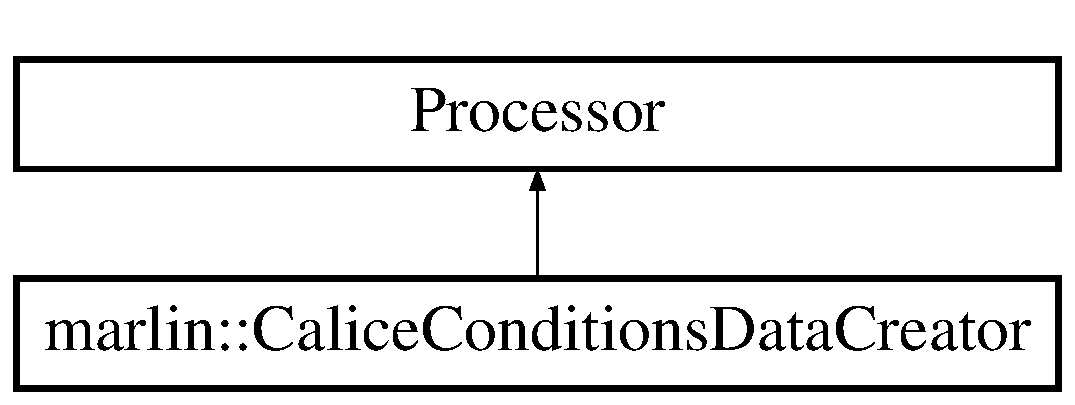
\includegraphics[height=2.000000cm]{classmarlin_1_1CaliceConditionsDataCreator}
\end{center}
\end{figure}
\subsection*{Public Member Functions}
\begin{DoxyCompactItemize}
\item 
Processor $\ast$ {\bfseries new\-Processor} ()\label{classmarlin_1_1CaliceConditionsDataCreator_a602c419bdb5c11770dd620711941f175}

\item 
void {\bf init} ()
\begin{DoxyCompactList}\small\item\em Install conditions change listener. \end{DoxyCompactList}\item 
void {\bfseries process\-Run\-Header} (L\-C\-Run\-Header $\ast$run)\label{classmarlin_1_1CaliceConditionsDataCreator_add37acebb16fb3faa09f17afa353ad6a}

\item 
void {\bf process\-Event} (L\-C\-Event $\ast$evt\-P)\label{classmarlin_1_1CaliceConditionsDataCreator_a1a7b0067f58a6376ab5e9ba73d389280}

\begin{DoxyCompactList}\small\item\em Update conditions data (not yet). \end{DoxyCompactList}\item 
void {\bfseries end} ()\label{classmarlin_1_1CaliceConditionsDataCreator_a7903f04212f4cbb7f95fecd657c289f0}

\end{DoxyCompactItemize}
\subsection*{Protected Types}
\begin{DoxyCompactItemize}
\item 
enum \{ \\*
{\bfseries k\-Ahc\-Module\-Location}, 
{\bfseries k\-Ahc\-Module\-Connection}, 
{\bfseries k\-Ahc\-Module\-Description}, 
{\bfseries k\-Emc\-Module\-Location}, 
\\*
{\bfseries k\-Emc\-Module\-Connection}, 
{\bfseries k\-Emc\-Module\-Description}, 
{\bfseries k\-Drift\-Chamber\-Parameter}, 
{\bfseries k\-Trigger\-Assignment}, 
\\*
{\bfseries k\-Trigger\-Check}, 
{\bfseries k\-Experimental\-Setup}, 
{\bfseries k\-N\-Collections}
 \}
\end{DoxyCompactItemize}
\subsection*{Protected Attributes}
\begin{DoxyCompactItemize}
\item 
std\-::string {\bfseries \-\_\-col\-Name} [k\-N\-Collections]\label{classmarlin_1_1CaliceConditionsDataCreator_a1c7c2ec9238554a06a8850b0679b66f9}

\item 
std\-::vector$<$ std\-::string $>$ {\bfseries \-\_\-input\-File\-Name} [k\-N\-Collections]\label{classmarlin_1_1CaliceConditionsDataCreator_a91361a635c7673038c4482ad8209f639}

\item 
std\-::vector$<$ std\-::string $>$ {\bfseries \-\_\-since\-Till\-Time} [k\-N\-Collections]\label{classmarlin_1_1CaliceConditionsDataCreator_a5dd2783bec7e29c83911b2c62a5733ea}

\item 
std\-::vector$<$ U\-T\-I\-L\-::\-L\-C\-Time $>$ {\bfseries \-\_\-since} [k\-N\-Collections]\label{classmarlin_1_1CaliceConditionsDataCreator_afb8943272775c52775822d64f0445505}

\item 
std\-::vector$<$ U\-T\-I\-L\-::\-L\-C\-Time $>$ {\bfseries \-\_\-till} [k\-N\-Collections]\label{classmarlin_1_1CaliceConditionsDataCreator_a6c8842188702a4d711ece614f93c0d88}

\item 
std\-::vector$<$ std\-::string $>$ {\bf \-\_\-beam\-Type}
\begin{DoxyCompactList}\small\item\em the nominal beam type. \end{DoxyCompactList}\item 
std\-::vector$<$ float $>$ {\bf \-\_\-beam\-Energy}
\begin{DoxyCompactList}\small\item\em nominal beam energy. \end{DoxyCompactList}\item 
std\-::vector$<$ float $>$ {\bf \-\_\-configuration\-Angle}
\begin{DoxyCompactList}\small\item\em angle between the detector normal and the beam axis. \end{DoxyCompactList}\item 
std\-::vector$<$ int $>$ {\bf \-\_\-trigger\-Main\-Word}
\begin{DoxyCompactList}\small\item\em position of the trigger main word in th fifo. \end{DoxyCompactList}\item 
std\-::vector$<$ int $>$ {\bf \-\_\-trigger\-Main\-Word\-Tolerance}\label{classmarlin_1_1CaliceConditionsDataCreator_ae121828e72a6e69229ea1102e3cacc4c}

\begin{DoxyCompactList}\small\item\em the tolerance on the trigger main word position \end{DoxyCompactList}\item 
std\-::vector$<$ int $>$ {\bf \-\_\-trigger\-Search\-Range}
\begin{DoxyCompactList}\small\item\em search range around the trigger main word which is search for overlapping triggers. \end{DoxyCompactList}\item 
lccd\-::\-I\-Conditions\-Handler $\ast$ {\bfseries \-\_\-conddb\-Handler} [k\-N\-Collections]\label{classmarlin_1_1CaliceConditionsDataCreator_ac99c9b4383bf7e786b763f5789147b1c}

\item 
std\-::vector\\*
$<$ E\-V\-E\-N\-T\-::\-L\-C\-Collection $\ast$ $>$ {\bfseries \-\_\-conddb\-Col} [k\-N\-Collections]\label{classmarlin_1_1CaliceConditionsDataCreator_a115c3f1d7deec6ab19666acff4be962e}

\item 
U\-T\-I\-L\-::\-L\-C\-Time {\bfseries \-\_\-valid\-Since}\label{classmarlin_1_1CaliceConditionsDataCreator_aa0271519445413603682631355db7a63}

\item 
U\-T\-I\-L\-::\-L\-C\-Time {\bfseries \-\_\-valid\-Till}\label{classmarlin_1_1CaliceConditionsDataCreator_a39ed98e58fe973f45aedbbf64a3aef2e}

\end{DoxyCompactItemize}
\subsection*{Static Protected Attributes}
\begin{DoxyCompactItemize}
\item 
static const char $\ast$ {\bfseries \-\_\-\-\_\-beam\-Type\-Names} [11]\label{classmarlin_1_1CaliceConditionsDataCreator_a86e1060f18685fd8e77e84a396b9004f}

\item 
static const char $\ast$ {\bfseries \-\_\-\-\_\-collection\-Names} [k\-N\-Collections]\label{classmarlin_1_1CaliceConditionsDataCreator_a828d149c7eaaa7c07aa28ccd2bcffd69}

\item 
static Create\-Coll\-Func\-\_\-t {\bfseries \-\_\-\-\_\-create\-Func} [k\-N\-Collections]\label{classmarlin_1_1CaliceConditionsDataCreator_a50bb1fc9365a24fde378c286a30cd47b}

\end{DoxyCompactItemize}
\subsection*{Friends}
\begin{DoxyCompactItemize}
\item 
class {\bfseries C\-A\-L\-I\-C\-E\-::\-Conditions\-Data\-Write\-Handler}\label{classmarlin_1_1CaliceConditionsDataCreator_a0e401bb1bfedeba5808934499877adf4}

\end{DoxyCompactItemize}


\subsection{Detailed Description}
Marlin processr which creates calice conditions data and makes them via a simplefile handler available. 

The processor creates\-: 
\begin{DoxyEnumerate}
\item Module\-Connection 
\item Module\-Location 
\item Module\-Description 
\item Drift\-Chamber\-Parameter 
\item Experimental\-Setup 
\item Trigger\-Assignament 
\end{DoxyEnumerate}collections. The creation of each collection can be individually steered. 

Definition at line 39 of file Calice\-Conditions\-Data\-Creator.\-hh.



\subsection{Member Function Documentation}
\index{marlin\-::\-Calice\-Conditions\-Data\-Creator@{marlin\-::\-Calice\-Conditions\-Data\-Creator}!init@{init}}
\index{init@{init}!marlin::CaliceConditionsDataCreator@{marlin\-::\-Calice\-Conditions\-Data\-Creator}}
\subsubsection[{init}]{\setlength{\rightskip}{0pt plus 5cm}void marlin\-::\-Calice\-Conditions\-Data\-Creator\-::init (
\begin{DoxyParamCaption}
{}
\end{DoxyParamCaption}
)}\label{classmarlin_1_1CaliceConditionsDataCreator_a53e34b9c420e45dda6bbab5f9f4400cc}


Install conditions change listener. 

The listeners are installed for the conditions data specified by the processor parameters. 

\subsection{Field Documentation}
\index{marlin\-::\-Calice\-Conditions\-Data\-Creator@{marlin\-::\-Calice\-Conditions\-Data\-Creator}!\-\_\-beam\-Energy@{\-\_\-beam\-Energy}}
\index{\-\_\-beam\-Energy@{\-\_\-beam\-Energy}!marlin::CaliceConditionsDataCreator@{marlin\-::\-Calice\-Conditions\-Data\-Creator}}
\subsubsection[{\-\_\-beam\-Energy}]{\setlength{\rightskip}{0pt plus 5cm}std\-::vector$<$float$>$ marlin\-::\-Calice\-Conditions\-Data\-Creator\-::\-\_\-beam\-Energy\hspace{0.3cm}{\ttfamily [protected]}}\label{classmarlin_1_1CaliceConditionsDataCreator_af8aa319f5771ba7bfcf4c3be1c36cf4f}


nominal beam energy. 



Definition at line 75 of file Calice\-Conditions\-Data\-Creator.\-hh.

\index{marlin\-::\-Calice\-Conditions\-Data\-Creator@{marlin\-::\-Calice\-Conditions\-Data\-Creator}!\-\_\-beam\-Type@{\-\_\-beam\-Type}}
\index{\-\_\-beam\-Type@{\-\_\-beam\-Type}!marlin::CaliceConditionsDataCreator@{marlin\-::\-Calice\-Conditions\-Data\-Creator}}
\subsubsection[{\-\_\-beam\-Type}]{\setlength{\rightskip}{0pt plus 5cm}std\-::vector$<$std\-::string$>$ marlin\-::\-Calice\-Conditions\-Data\-Creator\-::\-\_\-beam\-Type\hspace{0.3cm}{\ttfamily [protected]}}\label{classmarlin_1_1CaliceConditionsDataCreator_a0c0658ad562522454b5c278757e02118}


the nominal beam type. 



Definition at line 74 of file Calice\-Conditions\-Data\-Creator.\-hh.

\index{marlin\-::\-Calice\-Conditions\-Data\-Creator@{marlin\-::\-Calice\-Conditions\-Data\-Creator}!\-\_\-configuration\-Angle@{\-\_\-configuration\-Angle}}
\index{\-\_\-configuration\-Angle@{\-\_\-configuration\-Angle}!marlin::CaliceConditionsDataCreator@{marlin\-::\-Calice\-Conditions\-Data\-Creator}}
\subsubsection[{\-\_\-configuration\-Angle}]{\setlength{\rightskip}{0pt plus 5cm}std\-::vector$<$float$>$ marlin\-::\-Calice\-Conditions\-Data\-Creator\-::\-\_\-configuration\-Angle\hspace{0.3cm}{\ttfamily [protected]}}\label{classmarlin_1_1CaliceConditionsDataCreator_ae54f3d9bb7f189e2b888c1f3a5aac59c}


angle between the detector normal and the beam axis. 



Definition at line 76 of file Calice\-Conditions\-Data\-Creator.\-hh.

\index{marlin\-::\-Calice\-Conditions\-Data\-Creator@{marlin\-::\-Calice\-Conditions\-Data\-Creator}!\-\_\-trigger\-Main\-Word@{\-\_\-trigger\-Main\-Word}}
\index{\-\_\-trigger\-Main\-Word@{\-\_\-trigger\-Main\-Word}!marlin::CaliceConditionsDataCreator@{marlin\-::\-Calice\-Conditions\-Data\-Creator}}
\subsubsection[{\-\_\-trigger\-Main\-Word}]{\setlength{\rightskip}{0pt plus 5cm}std\-::vector$<$int$>$ marlin\-::\-Calice\-Conditions\-Data\-Creator\-::\-\_\-trigger\-Main\-Word\hspace{0.3cm}{\ttfamily [protected]}}\label{classmarlin_1_1CaliceConditionsDataCreator_a0459f44af2be6a6c11e129ec7a0f053c}


position of the trigger main word in th fifo. 



Definition at line 78 of file Calice\-Conditions\-Data\-Creator.\-hh.

\index{marlin\-::\-Calice\-Conditions\-Data\-Creator@{marlin\-::\-Calice\-Conditions\-Data\-Creator}!\-\_\-trigger\-Search\-Range@{\-\_\-trigger\-Search\-Range}}
\index{\-\_\-trigger\-Search\-Range@{\-\_\-trigger\-Search\-Range}!marlin::CaliceConditionsDataCreator@{marlin\-::\-Calice\-Conditions\-Data\-Creator}}
\subsubsection[{\-\_\-trigger\-Search\-Range}]{\setlength{\rightskip}{0pt plus 5cm}std\-::vector$<$int$>$ marlin\-::\-Calice\-Conditions\-Data\-Creator\-::\-\_\-trigger\-Search\-Range\hspace{0.3cm}{\ttfamily [protected]}}\label{classmarlin_1_1CaliceConditionsDataCreator_a0e3e6e12b1a9177d4c233719db4978ca}


search range around the trigger main word which is search for overlapping triggers. 



Definition at line 80 of file Calice\-Conditions\-Data\-Creator.\-hh.



The documentation for this class was generated from the following file\-:\begin{DoxyCompactItemize}
\item 
Calice\-Conditions\-Data\-Creator.\-hh\end{DoxyCompactItemize}

\section{C\-A\-L\-I\-C\-E\-:\-:Calice\-Ecal\-Calibration Class Reference}
\label{classCALICE_1_1CaliceEcalCalibration}\index{C\-A\-L\-I\-C\-E\-::\-Calice\-Ecal\-Calibration@{C\-A\-L\-I\-C\-E\-::\-Calice\-Ecal\-Calibration}}


\doxyref{Calibration}{p.}{classCalibration} of the Calice E\-C\-A\-L modules.  




{\ttfamily \#include $<$Calice\-Ecal\-Calibration.\-hh$>$}

Inheritance diagram for C\-A\-L\-I\-C\-E\-:\-:Calice\-Ecal\-Calibration\-:\begin{figure}[H]
\begin{center}
\leavevmode
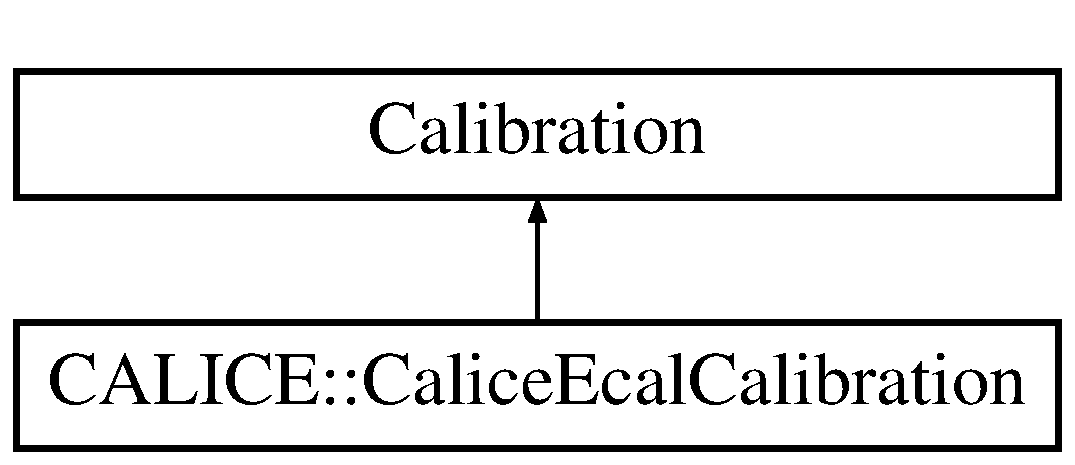
\includegraphics[height=2.000000cm]{classCALICE_1_1CaliceEcalCalibration}
\end{center}
\end{figure}
\subsection*{Public Member Functions}
\begin{DoxyCompactItemize}
\item 
{\bf noexcept} (false)
\begin{DoxyCompactList}\small\item\em Create the calibration object for the Calice Ecal. \end{DoxyCompactList}\item 
{\bf $\sim$\-Calice\-Ecal\-Calibration} ()
\begin{DoxyCompactList}\small\item\em Destructor. \end{DoxyCompactList}\item 
Float\-\_\-t {\bf get\-Calibrated\-Value} (U\-Int\-\_\-t module\-\_\-id, U\-Int\-\_\-t module\-\_\-type, U\-Int\-\_\-t cell\-\_\-index, Float\-\_\-t adc\-\_\-value) const 
\begin{DoxyCompactList}\small\item\em Determine from a pedestal subtracted A\-D\-C value a calibrated value. \end{DoxyCompactList}\item 
Bool\-\_\-t {\bf is\-Valid} (U\-Int\-\_\-t module\-\_\-id, U\-Int\-\_\-t module\-\_\-type, U\-Int\-\_\-t cell\-\_\-index) const 
\begin{DoxyCompactList}\small\item\em Return true if a the calibration constants for the given cell are in the allowed range. \end{DoxyCompactList}\item 
Bool\-\_\-t {\bf check\-For\-Calibration\-Constants\-Of\-Module} (U\-Int\-\_\-t module\-\_\-id, U\-Int\-\_\-t module\-\_\-type, U\-Int\-\_\-t n\-\_\-cells) const 
\begin{DoxyCompactList}\small\item\em Verify that calibration constants exist for a certain module. \end{DoxyCompactList}\item 
Int\-\_\-t {\bf get\-Minium\-A\-D\-C\-For\-Mip\-Threshold} (Float\-\_\-t mip\-\_\-energy\-\_\-fraction) const 
\begin{DoxyCompactList}\small\item\em Get the minimum adc value mips will have for the given energy fraction on all pads. \end{DoxyCompactList}\item 
void {\bf module\-Type\-Changed} (lcio\-::\-L\-C\-Collection $\ast$col)
\begin{DoxyCompactList}\small\item\em Notify the calibration object in case the definition of the module types has changed. \end{DoxyCompactList}\item 
void {\bf calibration\-Constant\-Changed} (lcio\-::\-L\-C\-Collection $\ast$col)
\begin{DoxyCompactList}\small\item\em Notify the calibration object when ever the calibration constants change. \end{DoxyCompactList}\end{DoxyCompactItemize}
\subsection*{Private Types}
\begin{DoxyCompactItemize}
\item 
typedef std\-::vector\\*
$<$ Ecal\-Module\-Calibration $>$ {\bfseries Module\-Type\-Calibration\-Constant\-List\-\_\-t}\label{classCALICE_1_1CaliceEcalCalibration_a7c5d9af5b11b804071982e5292422646}

\item 
typedef std\-::vector$<$ std\-::pair\\*
$<$ const \\*
Module\-Type\-Calibration\-Constant\-List\-\_\-t \\*
$\ast$, std\-::string $>$ $>$ {\bfseries Calibration\-Constant\-Per\-Type\-List\-\_\-t}\label{classCALICE_1_1CaliceEcalCalibration_aab75d417a8477f123384473c932b1d3e}

\end{DoxyCompactItemize}
\subsection*{Private Attributes}
\begin{DoxyCompactItemize}
\item 
std\-::map$<$ std\-::string, \\*
Module\-Type\-Calibration\-Constant\-List\-\_\-t $>$ {\bfseries \-\_\-calibration\-Constants}\label{classCALICE_1_1CaliceEcalCalibration_a3a4ba7bfc9da0dcae8acc075f74eff24}

\item 
Calibration\-Constant\-Per\-Type\-List\-\_\-t {\bf \-\_\-calibration\-Constants\-Per\-Type}
\begin{DoxyCompactList}\small\item\em \doxyref{Calibration}{p.}{classCalibration} constatns per Module. \end{DoxyCompactList}\item 
Conditions\-Change\-Delegator\\*
$<$ {\bf Calice\-Ecal\-Calibration} $>$ {\bfseries \-\_\-module\-Type\-Change}\label{classCALICE_1_1CaliceEcalCalibration_a49a0c1cccc53314ec3e8e44a7186031d}

\item 
Conditions\-Change\-Delegator\\*
$<$ {\bf Calice\-Ecal\-Calibration} $>$ {\bfseries \-\_\-calibration\-Constant\-Change}\label{classCALICE_1_1CaliceEcalCalibration_a3c8999e65ff7276c3acdeb7b19eeea0c}

\item 
Float\-\_\-t {\bfseries \-\_\-min\-Inv\-Calibration\-Constant}\label{classCALICE_1_1CaliceEcalCalibration_ac9690f336fa6c193427f12d4504ad6b4}

\end{DoxyCompactItemize}
\subsection*{Static Private Attributes}
\begin{DoxyCompactItemize}
\item 
static Ecal\-Module\-Calibration {\bf \-\_\-empty}
\begin{DoxyCompactList}\small\item\em Used to initialise the vector. \end{DoxyCompactList}\end{DoxyCompactItemize}


\subsection{Detailed Description}
\doxyref{Calibration}{p.}{classCalibration} of the Calice E\-C\-A\-L modules. 

Definition at line 18 of file Calice\-Ecal\-Calibration.\-hh.



\subsection{Constructor \& Destructor Documentation}
\index{C\-A\-L\-I\-C\-E\-::\-Calice\-Ecal\-Calibration@{C\-A\-L\-I\-C\-E\-::\-Calice\-Ecal\-Calibration}!$\sim$\-Calice\-Ecal\-Calibration@{$\sim$\-Calice\-Ecal\-Calibration}}
\index{$\sim$\-Calice\-Ecal\-Calibration@{$\sim$\-Calice\-Ecal\-Calibration}!CALICE::CaliceEcalCalibration@{C\-A\-L\-I\-C\-E\-::\-Calice\-Ecal\-Calibration}}
\subsubsection[{$\sim$\-Calice\-Ecal\-Calibration}]{\setlength{\rightskip}{0pt plus 5cm}C\-A\-L\-I\-C\-E\-::\-Calice\-Ecal\-Calibration\-::$\sim$\-Calice\-Ecal\-Calibration (
\begin{DoxyParamCaption}
{}
\end{DoxyParamCaption}
)\hspace{0.3cm}{\ttfamily [inline]}}\label{classCALICE_1_1CaliceEcalCalibration_a90c221567561015797ff5c1b035dda71}


Destructor. 

F\-I\-X\-M\-E\-: The destructor should deregister the conditions change handler. Unfortuneatly, this is not forseen in the Conditions Processor. 

Definition at line 32 of file Calice\-Ecal\-Calibration.\-hh.



\subsection{Member Function Documentation}
\index{C\-A\-L\-I\-C\-E\-::\-Calice\-Ecal\-Calibration@{C\-A\-L\-I\-C\-E\-::\-Calice\-Ecal\-Calibration}!calibration\-Constant\-Changed@{calibration\-Constant\-Changed}}
\index{calibration\-Constant\-Changed@{calibration\-Constant\-Changed}!CALICE::CaliceEcalCalibration@{C\-A\-L\-I\-C\-E\-::\-Calice\-Ecal\-Calibration}}
\subsubsection[{calibration\-Constant\-Changed}]{\setlength{\rightskip}{0pt plus 5cm}void C\-A\-L\-I\-C\-E\-::\-Calice\-Ecal\-Calibration\-::calibration\-Constant\-Changed (
\begin{DoxyParamCaption}
\item[{lcio\-::\-L\-C\-Collection $\ast$}]{col}
\end{DoxyParamCaption}
)}\label{classCALICE_1_1CaliceEcalCalibration_a0a82a3215a4e35f444904cb80cea3f46}


Notify the calibration object when ever the calibration constants change. 

This function must be called at least once before \doxyref{get\-Calibrated\-Value()}{p.}{classCALICE_1_1CaliceEcalCalibration_a4ffba5606c463a2b7419e85bc9008853} is used. 

Definition at line 121 of file Calice\-Ecal\-Calibration.\-cc.



References \-\_\-calibration\-Constants\-Per\-Type, and \-\_\-empty.

\index{C\-A\-L\-I\-C\-E\-::\-Calice\-Ecal\-Calibration@{C\-A\-L\-I\-C\-E\-::\-Calice\-Ecal\-Calibration}!check\-For\-Calibration\-Constants\-Of\-Module@{check\-For\-Calibration\-Constants\-Of\-Module}}
\index{check\-For\-Calibration\-Constants\-Of\-Module@{check\-For\-Calibration\-Constants\-Of\-Module}!CALICE::CaliceEcalCalibration@{C\-A\-L\-I\-C\-E\-::\-Calice\-Ecal\-Calibration}}
\subsubsection[{check\-For\-Calibration\-Constants\-Of\-Module}]{\setlength{\rightskip}{0pt plus 5cm}Bool\-\_\-t C\-A\-L\-I\-C\-E\-::\-Calice\-Ecal\-Calibration\-::check\-For\-Calibration\-Constants\-Of\-Module (
\begin{DoxyParamCaption}
\item[{U\-Int\-\_\-t}]{module\-\_\-id, }
\item[{U\-Int\-\_\-t}]{module\-\_\-type, }
\item[{U\-Int\-\_\-t}]{n\-\_\-cells}
\end{DoxyParamCaption}
) const\hspace{0.3cm}{\ttfamily [inline]}}\label{classCALICE_1_1CaliceEcalCalibration_ae6cb1b990f7c4eb7dc274089df464772}


Verify that calibration constants exist for a certain module. 


\begin{DoxyParams}{Parameters}
{\em module\-\_\-id} & id Or serial number of a module which uniquely identifies a detector module of a certain type. \\
\hline
{\em module\-\_\-type} & the type of the detector module \\
\hline
{\em n\-\_\-cells} & the number of cells on this module. Return true if calibration constants exist for the given module and the number of cells matches the number of calibration constants. \\
\hline
\end{DoxyParams}


Definition at line 99 of file Calice\-Ecal\-Calibration.\-hh.



References \-\_\-calibration\-Constants\-Per\-Type.

\index{C\-A\-L\-I\-C\-E\-::\-Calice\-Ecal\-Calibration@{C\-A\-L\-I\-C\-E\-::\-Calice\-Ecal\-Calibration}!get\-Calibrated\-Value@{get\-Calibrated\-Value}}
\index{get\-Calibrated\-Value@{get\-Calibrated\-Value}!CALICE::CaliceEcalCalibration@{C\-A\-L\-I\-C\-E\-::\-Calice\-Ecal\-Calibration}}
\subsubsection[{get\-Calibrated\-Value}]{\setlength{\rightskip}{0pt plus 5cm}Float\-\_\-t C\-A\-L\-I\-C\-E\-::\-Calice\-Ecal\-Calibration\-::get\-Calibrated\-Value (
\begin{DoxyParamCaption}
\item[{U\-Int\-\_\-t}]{module\-\_\-id, }
\item[{U\-Int\-\_\-t}]{module\-\_\-type, }
\item[{U\-Int\-\_\-t}]{cell\-\_\-index, }
\item[{Float\-\_\-t}]{adc\-\_\-value}
\end{DoxyParamCaption}
) const\hspace{0.3cm}{\ttfamily [inline]}}\label{classCALICE_1_1CaliceEcalCalibration_a4ffba5606c463a2b7419e85bc9008853}


Determine from a pedestal subtracted A\-D\-C value a calibrated value. 


\begin{DoxyParams}{Parameters}
{\em module\-\_\-id} & id Or serial number of a module which uniquely identifies a detector module of a certain type. \\
\hline
{\em module\-\_\-type} & the type of the detector module \\
\hline
{\em cell\-\_\-index} & the cell\-\_\-index in read order\-: first the A\-D\-C values of the first sample from all chips, then the next sample ... \\
\hline
{\em adc\-\_\-value} & the A\-D\-C value which should be calibrated. \\
\hline
\end{DoxyParams}
\begin{DoxyReturn}{Returns}
the calibrated value. 
\end{DoxyReturn}


Definition at line 42 of file Calice\-Ecal\-Calibration.\-hh.



References \-\_\-calibration\-Constants\-Per\-Type.

\index{C\-A\-L\-I\-C\-E\-::\-Calice\-Ecal\-Calibration@{C\-A\-L\-I\-C\-E\-::\-Calice\-Ecal\-Calibration}!get\-Minium\-A\-D\-C\-For\-Mip\-Threshold@{get\-Minium\-A\-D\-C\-For\-Mip\-Threshold}}
\index{get\-Minium\-A\-D\-C\-For\-Mip\-Threshold@{get\-Minium\-A\-D\-C\-For\-Mip\-Threshold}!CALICE::CaliceEcalCalibration@{C\-A\-L\-I\-C\-E\-::\-Calice\-Ecal\-Calibration}}
\subsubsection[{get\-Minium\-A\-D\-C\-For\-Mip\-Threshold}]{\setlength{\rightskip}{0pt plus 5cm}Int\-\_\-t C\-A\-L\-I\-C\-E\-::\-Calice\-Ecal\-Calibration\-::get\-Minium\-A\-D\-C\-For\-Mip\-Threshold (
\begin{DoxyParamCaption}
\item[{Float\-\_\-t}]{mip\-\_\-energy\-\_\-fraction}
\end{DoxyParamCaption}
) const\hspace{0.3cm}{\ttfamily [inline]}}\label{classCALICE_1_1CaliceEcalCalibration_af23ff60b95893d5ab5c09132c678805d}


Get the minimum adc value mips will have for the given energy fraction on all pads. 


\begin{DoxyParams}{Parameters}
{\em mip\-\_\-energy\-\_\-fraction} & the energy in mips \\
\hline
\end{DoxyParams}
\begin{DoxyReturn}{Returns}
minimum adc value which is below the given energy on all pads. This method can be used to get the lowest adc value a mip of the given energy fraction will have on all pads. This value is useful to select candidates before actually performing th calibration. This function is intended to be called at the beginning of each event. 
\end{DoxyReturn}


Definition at line 114 of file Calice\-Ecal\-Calibration.\-hh.

\index{C\-A\-L\-I\-C\-E\-::\-Calice\-Ecal\-Calibration@{C\-A\-L\-I\-C\-E\-::\-Calice\-Ecal\-Calibration}!is\-Valid@{is\-Valid}}
\index{is\-Valid@{is\-Valid}!CALICE::CaliceEcalCalibration@{C\-A\-L\-I\-C\-E\-::\-Calice\-Ecal\-Calibration}}
\subsubsection[{is\-Valid}]{\setlength{\rightskip}{0pt plus 5cm}Bool\-\_\-t C\-A\-L\-I\-C\-E\-::\-Calice\-Ecal\-Calibration\-::is\-Valid (
\begin{DoxyParamCaption}
\item[{U\-Int\-\_\-t}]{module\-\_\-id, }
\item[{U\-Int\-\_\-t}]{module\-\_\-type, }
\item[{U\-Int\-\_\-t}]{cell\-\_\-index}
\end{DoxyParamCaption}
) const\hspace{0.3cm}{\ttfamily [inline]}}\label{classCALICE_1_1CaliceEcalCalibration_a15dc169487e5d13c4da34f56387f2218}


Return true if a the calibration constants for the given cell are in the allowed range. 


\begin{DoxyParams}{Parameters}
{\em module\-\_\-id} & id Or serial number of a module which uniquely identifies a detector module of a certain type. \\
\hline
{\em module\-\_\-type} & the type of the detector module \\
\hline
{\em cell\-\_\-index} & the cell\-\_\-index in read order\-: first the A\-D\-C values of the first sample from all chips, then the next sample ... \\
\hline
\end{DoxyParams}
\begin{DoxyReturn}{Returns}
true for cells with valid calibration constants, false for cells which should be declared dead.
\end{DoxyReturn}
This method is used to find, after module connection changes, cells which should be declared dead. 

Definition at line 68 of file Calice\-Ecal\-Calibration.\-hh.



References \-\_\-calibration\-Constants\-Per\-Type.

\index{C\-A\-L\-I\-C\-E\-::\-Calice\-Ecal\-Calibration@{C\-A\-L\-I\-C\-E\-::\-Calice\-Ecal\-Calibration}!module\-Type\-Changed@{module\-Type\-Changed}}
\index{module\-Type\-Changed@{module\-Type\-Changed}!CALICE::CaliceEcalCalibration@{C\-A\-L\-I\-C\-E\-::\-Calice\-Ecal\-Calibration}}
\subsubsection[{module\-Type\-Changed}]{\setlength{\rightskip}{0pt plus 5cm}void C\-A\-L\-I\-C\-E\-::\-Calice\-Ecal\-Calibration\-::module\-Type\-Changed (
\begin{DoxyParamCaption}
\item[{lcio\-::\-L\-C\-Collection $\ast$}]{col}
\end{DoxyParamCaption}
)}\label{classCALICE_1_1CaliceEcalCalibration_ab29f2d5fdc65d38388ca8d3a57f3a419}


Notify the calibration object in case the definition of the module types has changed. 

This function must be called at least once before \doxyref{get\-Calibrated\-Value()}{p.}{classCALICE_1_1CaliceEcalCalibration_a4ffba5606c463a2b7419e85bc9008853} is used. 

Definition at line 79 of file Calice\-Ecal\-Calibration.\-cc.



References \-\_\-calibration\-Constants\-Per\-Type.

\index{C\-A\-L\-I\-C\-E\-::\-Calice\-Ecal\-Calibration@{C\-A\-L\-I\-C\-E\-::\-Calice\-Ecal\-Calibration}!noexcept@{noexcept}}
\index{noexcept@{noexcept}!CALICE::CaliceEcalCalibration@{C\-A\-L\-I\-C\-E\-::\-Calice\-Ecal\-Calibration}}
\subsubsection[{noexcept}]{\setlength{\rightskip}{0pt plus 5cm}C\-A\-L\-I\-C\-E\-::\-Calice\-Ecal\-Calibration\-::noexcept (
\begin{DoxyParamCaption}
\item[{false}]{}
\end{DoxyParamCaption}
)}\label{classCALICE_1_1CaliceEcalCalibration_a649e0aadc09a6d76235dfc4fe9ff7dc1}


Create the calibration object for the Calice Ecal. 

The constructor will register handlers for conditions data changes\-: changes of the module types and the calibration constants. 

\subsection{Field Documentation}
\index{C\-A\-L\-I\-C\-E\-::\-Calice\-Ecal\-Calibration@{C\-A\-L\-I\-C\-E\-::\-Calice\-Ecal\-Calibration}!\-\_\-calibration\-Constants\-Per\-Type@{\-\_\-calibration\-Constants\-Per\-Type}}
\index{\-\_\-calibration\-Constants\-Per\-Type@{\-\_\-calibration\-Constants\-Per\-Type}!CALICE::CaliceEcalCalibration@{C\-A\-L\-I\-C\-E\-::\-Calice\-Ecal\-Calibration}}
\subsubsection[{\-\_\-calibration\-Constants\-Per\-Type}]{\setlength{\rightskip}{0pt plus 5cm}Calibration\-Constant\-Per\-Type\-List\-\_\-t C\-A\-L\-I\-C\-E\-::\-Calice\-Ecal\-Calibration\-::\-\_\-calibration\-Constants\-Per\-Type\hspace{0.3cm}{\ttfamily [private]}}\label{classCALICE_1_1CaliceEcalCalibration_ae5dc90ad764f76fc60628267eb5e5504}


\doxyref{Calibration}{p.}{classCalibration} constatns per Module. 

The first array component is the module type, the second the serial number of the module. 

Definition at line 135 of file Calice\-Ecal\-Calibration.\-hh.



Referenced by calibration\-Constant\-Changed(), check\-For\-Calibration\-Constants\-Of\-Module(), get\-Calibrated\-Value(), is\-Valid(), and module\-Type\-Changed().

\index{C\-A\-L\-I\-C\-E\-::\-Calice\-Ecal\-Calibration@{C\-A\-L\-I\-C\-E\-::\-Calice\-Ecal\-Calibration}!\-\_\-empty@{\-\_\-empty}}
\index{\-\_\-empty@{\-\_\-empty}!CALICE::CaliceEcalCalibration@{C\-A\-L\-I\-C\-E\-::\-Calice\-Ecal\-Calibration}}
\subsubsection[{\-\_\-empty}]{\setlength{\rightskip}{0pt plus 5cm}Ecal\-Module\-Calibration C\-A\-L\-I\-C\-E\-::\-Calice\-Ecal\-Calibration\-::\-\_\-empty\hspace{0.3cm}{\ttfamily [static]}, {\ttfamily [private]}}\label{classCALICE_1_1CaliceEcalCalibration_a659518967a2207c6cf2e216994450898}


Used to initialise the vector. 

Otherwise for each element for which the default constructor is called an object is created. 

Definition at line 141 of file Calice\-Ecal\-Calibration.\-hh.



Referenced by calibration\-Constant\-Changed().



The documentation for this class was generated from the following files\-:\begin{DoxyCompactItemize}
\item 
Calice\-Ecal\-Calibration.\-hh\item 
Calice\-Ecal\-Calibration.\-cc\end{DoxyCompactItemize}

\section{C\-A\-L\-I\-C\-E\-:\-:Calice\-Ecal\-Calibration\-Kit Class Reference}
\label{classCALICE_1_1CaliceEcalCalibrationKit}\index{C\-A\-L\-I\-C\-E\-::\-Calice\-Ecal\-Calibration\-Kit@{C\-A\-L\-I\-C\-E\-::\-Calice\-Ecal\-Calibration\-Kit}}


Create an Calice E\-C\-A\-L calibration object.  


Inheritance diagram for C\-A\-L\-I\-C\-E\-:\-:Calice\-Ecal\-Calibration\-Kit\-:\begin{figure}[H]
\begin{center}
\leavevmode
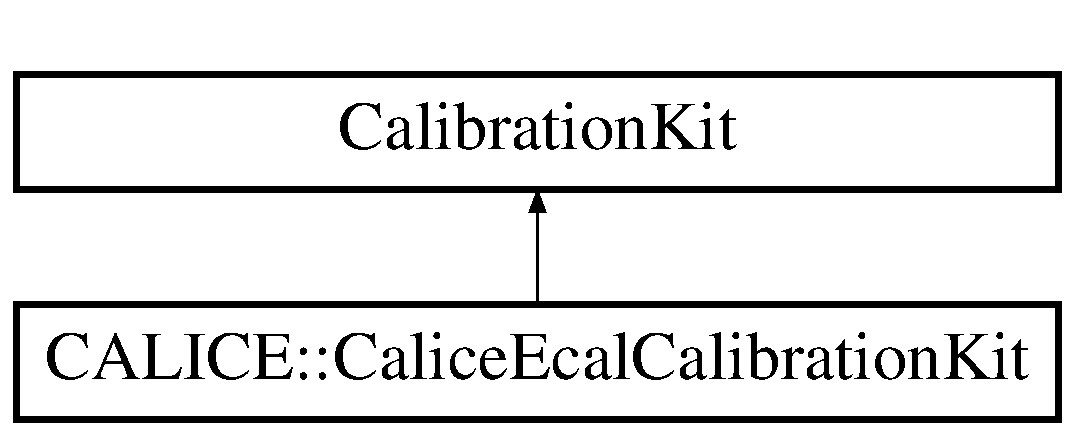
\includegraphics[height=2.000000cm]{classCALICE_1_1CaliceEcalCalibrationKit}
\end{center}
\end{figure}
\subsection*{Public Member Functions}
\begin{DoxyCompactItemize}
\item 
{\bf Calibration} $\ast$ {\bf create} (const std\-::string \&module\-\_\-type\-\_\-col\-\_\-name, const std\-::string \&module\-\_\-calibration\-\_\-col\-\_\-name) const 
\begin{DoxyCompactList}\small\item\em create calibration object. \end{DoxyCompactList}\end{DoxyCompactItemize}
\subsection*{Static Protected Attributes}
\begin{DoxyCompactItemize}
\item 
static {\bf Calice\-Ecal\-Calibration\-Kit} {\bfseries \-\_\-\-\_\-instance}\label{classCALICE_1_1CaliceEcalCalibrationKit_af2b31f371e49d2795d9ae1e3680a4863}

\end{DoxyCompactItemize}


\subsection{Detailed Description}
Create an Calice E\-C\-A\-L calibration object. 

\begin{DoxySeeAlso}{See Also}
\doxyref{Calice\-Ecal\-Calibration}{p.}{classCALICE_1_1CaliceEcalCalibration}. 
\end{DoxySeeAlso}


Definition at line 26 of file Calice\-Ecal\-Calibration.\-cc.



\subsection{Member Function Documentation}
\index{C\-A\-L\-I\-C\-E\-::\-Calice\-Ecal\-Calibration\-Kit@{C\-A\-L\-I\-C\-E\-::\-Calice\-Ecal\-Calibration\-Kit}!create@{create}}
\index{create@{create}!CALICE::CaliceEcalCalibrationKit@{C\-A\-L\-I\-C\-E\-::\-Calice\-Ecal\-Calibration\-Kit}}
\subsubsection[{create}]{\setlength{\rightskip}{0pt plus 5cm}{\bf Calibration}$\ast$ C\-A\-L\-I\-C\-E\-::\-Calice\-Ecal\-Calibration\-Kit\-::create (
\begin{DoxyParamCaption}
\item[{const std\-::string \&}]{module\-\_\-type\-\_\-col\-\_\-name, }
\item[{const std\-::string \&}]{module\-\_\-calibration\-\_\-col\-\_\-name}
\end{DoxyParamCaption}
) const\hspace{0.3cm}{\ttfamily [inline]}, {\ttfamily [virtual]}}\label{classCALICE_1_1CaliceEcalCalibrationKit_aa8754032807fe2e3d7d8dc4225464829}


create calibration object. 


\begin{DoxyParams}{Parameters}
{\em module\-\_\-type\-\_\-col\-\_\-name} & the name of the conditions data collection with the module types. \\
\hline
{\em module\-\_\-calibration\-\_\-col\-\_\-name} & the name of the conditions data collection which contains the calibration constants. F\-I\-X\-M\-E\-: There should be a better method to hand parameters to \doxyref{Calibration}{p.}{classCalibration} objects. \\
\hline
\end{DoxyParams}


Implements {\bf Calibration\-Kit} \doxyref{}{p.}{classCalibrationKit_ab3aea5671d91a7b6f5e839324cf45a70}.



Definition at line 36 of file Calice\-Ecal\-Calibration.\-cc.



The documentation for this class was generated from the following file\-:\begin{DoxyCompactItemize}
\item 
Calice\-Ecal\-Calibration.\-cc\end{DoxyCompactItemize}

\section{marlin\-:\-:Calice\-Trigger\-Processor Class Reference}
\label{classmarlin_1_1CaliceTriggerProcessor}\index{marlin\-::\-Calice\-Trigger\-Processor@{marlin\-::\-Calice\-Trigger\-Processor}}


Class which adds basic trigger information to the event parameters In order to make use of the trigger information this processor has to run {\itshape before} each other user defined processor.  




{\ttfamily \#include $<$Calice\-Trigger\-Processor.\-hh$>$}

Inheritance diagram for marlin\-:\-:Calice\-Trigger\-Processor\-:\begin{figure}[H]
\begin{center}
\leavevmode
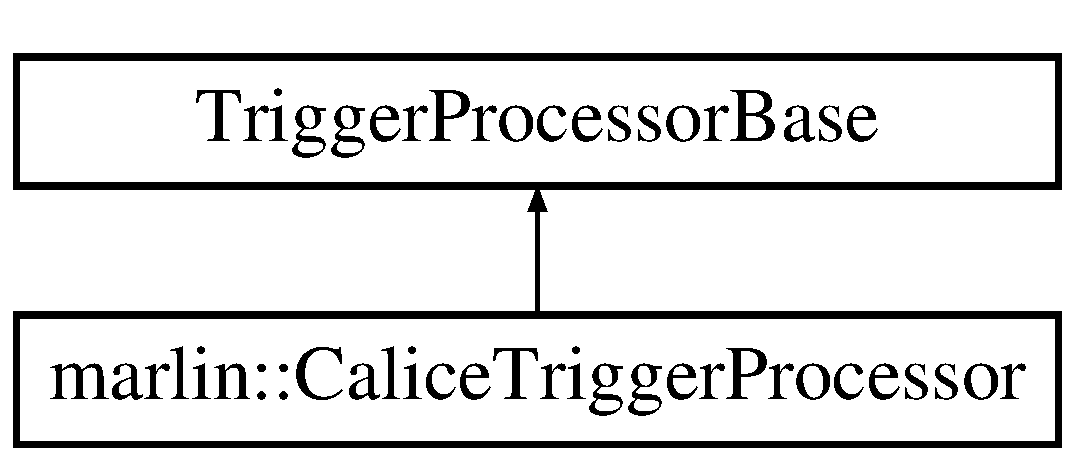
\includegraphics[height=2.000000cm]{classmarlin_1_1CaliceTriggerProcessor}
\end{center}
\end{figure}
\subsection*{Public Member Functions}
\begin{DoxyCompactItemize}
\item 
Processor $\ast$ {\bfseries new\-Processor} ()\label{classmarlin_1_1CaliceTriggerProcessor_a8ae7d8ea18ceb4047ebe26f2475e2f3b}

\item 
void {\bfseries init} ()\label{classmarlin_1_1CaliceTriggerProcessor_ad24c5897512a53e0147b25a23276c553}

\item 
void {\bfseries process\-Event} (L\-C\-Event $\ast$evt)\label{classmarlin_1_1CaliceTriggerProcessor_a4a2144796b9fb8b27ad713a462545878}

\item 
void {\bfseries end} ()\label{classmarlin_1_1CaliceTriggerProcessor_a75426b0c47cba668cc037e6ca19cd18b}

\end{DoxyCompactItemize}
\subsection*{Private Attributes}
\begin{DoxyCompactItemize}
\item 
std\-::string {\bf \-\_\-conf\-Trigger\-Bits\-Par\-Name}
\begin{DoxyCompactList}\small\item\em par. \end{DoxyCompactList}\item 
std\-::string {\bf \-\_\-event\-Trigger\-Bits\-Par\-Name}
\begin{DoxyCompactList}\small\item\em par. \end{DoxyCompactList}\item 
std\-::string {\bf \-\_\-par\-Name\-Trigger\-Main\-Word}
\begin{DoxyCompactList}\small\item\em Par. \end{DoxyCompactList}\item 
std\-::string {\bf \-\_\-par\-Name\-Trigger\-Post\-History}
\begin{DoxyCompactList}\small\item\em Par, name of the trigger post history. \end{DoxyCompactList}\item 
std\-::string {\bf \-\_\-par\-Name\-Trigger\-Pre\-History}
\begin{DoxyCompactList}\small\item\em Par, name of the trigger pre history. \end{DoxyCompactList}\item 
std\-::string {\bfseries \-\_\-par\-Name\-Trigger\-Post\-History\-Pos}\label{classmarlin_1_1CaliceTriggerProcessor_afc4b7bcc4eb2327e67df20cfedc5b668}

\item 
std\-::string {\bfseries \-\_\-par\-Name\-Trigger\-Post\-History\-Bits}\label{classmarlin_1_1CaliceTriggerProcessor_a06a31c9af414f0539c4504fa54079f67}

\item 
std\-::string {\bfseries \-\_\-par\-Name\-Trigger\-Pre\-History\-Pos}\label{classmarlin_1_1CaliceTriggerProcessor_afe63efbbcc0e17aa874778e909240ef4}

\item 
std\-::string {\bfseries \-\_\-par\-Name\-Trigger\-Pre\-History\-Bits}\label{classmarlin_1_1CaliceTriggerProcessor_a144777e561189e07ba32fb395de6daf4}

\item 
U\-Int\-\_\-t {\bf \-\_\-no\-Main\-Word}
\begin{DoxyCompactList}\small\item\em events for which the main word was not within the valid range. \end{DoxyCompactList}\item 
U\-Int\-\_\-t {\bf \-\_\-events\-With\-Out\-Of\-Range\-Triggers}
\begin{DoxyCompactList}\small\item\em events for which possible trigger bits were out of range. \end{DoxyCompactList}\item 
String\-Vec {\bf \-\_\-beam\-Trigger\-Names}
\begin{DoxyCompactList}\small\item\em Names of all trigger which indicated physics events and which will be ignored for pedestal calculation. \end{DoxyCompactList}\item 
unsigned int {\bf \-\_\-beam\-Trigger\-Bit\-Mask}
\begin{DoxyCompactList}\small\item\em Bit mask of all triggers which indicated physics events and which will be ignored for pedestal calculation. \end{DoxyCompactList}\item 
Int\-Vec {\bf \-\_\-no\-Trigger\-Activity\-Range}
\begin{DoxyCompactList}\small\item\em The time in ns before and after the main word during which there is no beam trigger allowed. \end{DoxyCompactList}\end{DoxyCompactItemize}


\subsection{Detailed Description}
Class which adds basic trigger information to the event parameters In order to make use of the trigger information this processor has to run {\itshape before} each other user defined processor. 

It initializes the trigger handler through which the user can obtain more information on trigger issues in other processors. Here it adds the trigger which have fired the event to the event parameters. This trigger information is made persistent with the event and can be later on used in higher level analysis. \begin{DoxyAuthor}{Author}
\-: R. P�schl D\-E\-S\-Y 
\end{DoxyAuthor}
\begin{DoxyDate}{Date}
Dec 7 2005 
\end{DoxyDate}


Definition at line 39 of file Calice\-Trigger\-Processor.\-hh.



\subsection{Field Documentation}
\index{marlin\-::\-Calice\-Trigger\-Processor@{marlin\-::\-Calice\-Trigger\-Processor}!\-\_\-beam\-Trigger\-Bit\-Mask@{\-\_\-beam\-Trigger\-Bit\-Mask}}
\index{\-\_\-beam\-Trigger\-Bit\-Mask@{\-\_\-beam\-Trigger\-Bit\-Mask}!marlin::CaliceTriggerProcessor@{marlin\-::\-Calice\-Trigger\-Processor}}
\subsubsection[{\-\_\-beam\-Trigger\-Bit\-Mask}]{\setlength{\rightskip}{0pt plus 5cm}unsigned int marlin\-::\-Calice\-Trigger\-Processor\-::\-\_\-beam\-Trigger\-Bit\-Mask\hspace{0.3cm}{\ttfamily [private]}}\label{classmarlin_1_1CaliceTriggerProcessor_a7bae04321ad0bf2fd8168bfaa2f13f52}


Bit mask of all triggers which indicated physics events and which will be ignored for pedestal calculation. 



Definition at line 65 of file Calice\-Trigger\-Processor.\-hh.

\index{marlin\-::\-Calice\-Trigger\-Processor@{marlin\-::\-Calice\-Trigger\-Processor}!\-\_\-beam\-Trigger\-Names@{\-\_\-beam\-Trigger\-Names}}
\index{\-\_\-beam\-Trigger\-Names@{\-\_\-beam\-Trigger\-Names}!marlin::CaliceTriggerProcessor@{marlin\-::\-Calice\-Trigger\-Processor}}
\subsubsection[{\-\_\-beam\-Trigger\-Names}]{\setlength{\rightskip}{0pt plus 5cm}String\-Vec marlin\-::\-Calice\-Trigger\-Processor\-::\-\_\-beam\-Trigger\-Names\hspace{0.3cm}{\ttfamily [private]}}\label{classmarlin_1_1CaliceTriggerProcessor_ae3443ac3f3dae23e9490552cb270d5f3}


Names of all trigger which indicated physics events and which will be ignored for pedestal calculation. 



Definition at line 64 of file Calice\-Trigger\-Processor.\-hh.

\index{marlin\-::\-Calice\-Trigger\-Processor@{marlin\-::\-Calice\-Trigger\-Processor}!\-\_\-conf\-Trigger\-Bits\-Par\-Name@{\-\_\-conf\-Trigger\-Bits\-Par\-Name}}
\index{\-\_\-conf\-Trigger\-Bits\-Par\-Name@{\-\_\-conf\-Trigger\-Bits\-Par\-Name}!marlin::CaliceTriggerProcessor@{marlin\-::\-Calice\-Trigger\-Processor}}
\subsubsection[{\-\_\-conf\-Trigger\-Bits\-Par\-Name}]{\setlength{\rightskip}{0pt plus 5cm}std\-::string marlin\-::\-Calice\-Trigger\-Processor\-::\-\_\-conf\-Trigger\-Bits\-Par\-Name\hspace{0.3cm}{\ttfamily [private]}}\label{classmarlin_1_1CaliceTriggerProcessor_a71283d68a025529d27f9b59d4939a8ff}


par. 

name of the configuration trigger bits. 

Definition at line 50 of file Calice\-Trigger\-Processor.\-hh.

\index{marlin\-::\-Calice\-Trigger\-Processor@{marlin\-::\-Calice\-Trigger\-Processor}!\-\_\-events\-With\-Out\-Of\-Range\-Triggers@{\-\_\-events\-With\-Out\-Of\-Range\-Triggers}}
\index{\-\_\-events\-With\-Out\-Of\-Range\-Triggers@{\-\_\-events\-With\-Out\-Of\-Range\-Triggers}!marlin::CaliceTriggerProcessor@{marlin\-::\-Calice\-Trigger\-Processor}}
\subsubsection[{\-\_\-events\-With\-Out\-Of\-Range\-Triggers}]{\setlength{\rightskip}{0pt plus 5cm}U\-Int\-\_\-t marlin\-::\-Calice\-Trigger\-Processor\-::\-\_\-events\-With\-Out\-Of\-Range\-Triggers\hspace{0.3cm}{\ttfamily [private]}}\label{classmarlin_1_1CaliceTriggerProcessor_a521a453cfb29f46ef79ba17121e89f6f}


events for which possible trigger bits were out of range. 



Definition at line 62 of file Calice\-Trigger\-Processor.\-hh.

\index{marlin\-::\-Calice\-Trigger\-Processor@{marlin\-::\-Calice\-Trigger\-Processor}!\-\_\-event\-Trigger\-Bits\-Par\-Name@{\-\_\-event\-Trigger\-Bits\-Par\-Name}}
\index{\-\_\-event\-Trigger\-Bits\-Par\-Name@{\-\_\-event\-Trigger\-Bits\-Par\-Name}!marlin::CaliceTriggerProcessor@{marlin\-::\-Calice\-Trigger\-Processor}}
\subsubsection[{\-\_\-event\-Trigger\-Bits\-Par\-Name}]{\setlength{\rightskip}{0pt plus 5cm}std\-::string marlin\-::\-Calice\-Trigger\-Processor\-::\-\_\-event\-Trigger\-Bits\-Par\-Name\hspace{0.3cm}{\ttfamily [private]}}\label{classmarlin_1_1CaliceTriggerProcessor_a90f8c6f9aecafda817964a4272c1bc82}


par. 

name of the event trigger bits. 

Definition at line 51 of file Calice\-Trigger\-Processor.\-hh.

\index{marlin\-::\-Calice\-Trigger\-Processor@{marlin\-::\-Calice\-Trigger\-Processor}!\-\_\-no\-Main\-Word@{\-\_\-no\-Main\-Word}}
\index{\-\_\-no\-Main\-Word@{\-\_\-no\-Main\-Word}!marlin::CaliceTriggerProcessor@{marlin\-::\-Calice\-Trigger\-Processor}}
\subsubsection[{\-\_\-no\-Main\-Word}]{\setlength{\rightskip}{0pt plus 5cm}U\-Int\-\_\-t marlin\-::\-Calice\-Trigger\-Processor\-::\-\_\-no\-Main\-Word\hspace{0.3cm}{\ttfamily [private]}}\label{classmarlin_1_1CaliceTriggerProcessor_a08d5438ca77dc832d115d7f3f73dba59}


events for which the main word was not within the valid range. 



Definition at line 61 of file Calice\-Trigger\-Processor.\-hh.

\index{marlin\-::\-Calice\-Trigger\-Processor@{marlin\-::\-Calice\-Trigger\-Processor}!\-\_\-no\-Trigger\-Activity\-Range@{\-\_\-no\-Trigger\-Activity\-Range}}
\index{\-\_\-no\-Trigger\-Activity\-Range@{\-\_\-no\-Trigger\-Activity\-Range}!marlin::CaliceTriggerProcessor@{marlin\-::\-Calice\-Trigger\-Processor}}
\subsubsection[{\-\_\-no\-Trigger\-Activity\-Range}]{\setlength{\rightskip}{0pt plus 5cm}Int\-Vec marlin\-::\-Calice\-Trigger\-Processor\-::\-\_\-no\-Trigger\-Activity\-Range\hspace{0.3cm}{\ttfamily [private]}}\label{classmarlin_1_1CaliceTriggerProcessor_ab54172955bbe9099625b548046dd79ea}


The time in ns before and after the main word during which there is no beam trigger allowed. 



Definition at line 66 of file Calice\-Trigger\-Processor.\-hh.

\index{marlin\-::\-Calice\-Trigger\-Processor@{marlin\-::\-Calice\-Trigger\-Processor}!\-\_\-par\-Name\-Trigger\-Main\-Word@{\-\_\-par\-Name\-Trigger\-Main\-Word}}
\index{\-\_\-par\-Name\-Trigger\-Main\-Word@{\-\_\-par\-Name\-Trigger\-Main\-Word}!marlin::CaliceTriggerProcessor@{marlin\-::\-Calice\-Trigger\-Processor}}
\subsubsection[{\-\_\-par\-Name\-Trigger\-Main\-Word}]{\setlength{\rightskip}{0pt plus 5cm}std\-::string marlin\-::\-Calice\-Trigger\-Processor\-::\-\_\-par\-Name\-Trigger\-Main\-Word\hspace{0.3cm}{\ttfamily [private]}}\label{classmarlin_1_1CaliceTriggerProcessor_a7c9c1511a3be17e49f6f416bea095eb4}


Par. 

name of the trigger main word. 

Definition at line 52 of file Calice\-Trigger\-Processor.\-hh.

\index{marlin\-::\-Calice\-Trigger\-Processor@{marlin\-::\-Calice\-Trigger\-Processor}!\-\_\-par\-Name\-Trigger\-Post\-History@{\-\_\-par\-Name\-Trigger\-Post\-History}}
\index{\-\_\-par\-Name\-Trigger\-Post\-History@{\-\_\-par\-Name\-Trigger\-Post\-History}!marlin::CaliceTriggerProcessor@{marlin\-::\-Calice\-Trigger\-Processor}}
\subsubsection[{\-\_\-par\-Name\-Trigger\-Post\-History}]{\setlength{\rightskip}{0pt plus 5cm}std\-::string marlin\-::\-Calice\-Trigger\-Processor\-::\-\_\-par\-Name\-Trigger\-Post\-History\hspace{0.3cm}{\ttfamily [private]}}\label{classmarlin_1_1CaliceTriggerProcessor_a6a1a2c84f826a0c56c5475c4ca79794b}


Par, name of the trigger post history. 



Definition at line 53 of file Calice\-Trigger\-Processor.\-hh.

\index{marlin\-::\-Calice\-Trigger\-Processor@{marlin\-::\-Calice\-Trigger\-Processor}!\-\_\-par\-Name\-Trigger\-Pre\-History@{\-\_\-par\-Name\-Trigger\-Pre\-History}}
\index{\-\_\-par\-Name\-Trigger\-Pre\-History@{\-\_\-par\-Name\-Trigger\-Pre\-History}!marlin::CaliceTriggerProcessor@{marlin\-::\-Calice\-Trigger\-Processor}}
\subsubsection[{\-\_\-par\-Name\-Trigger\-Pre\-History}]{\setlength{\rightskip}{0pt plus 5cm}std\-::string marlin\-::\-Calice\-Trigger\-Processor\-::\-\_\-par\-Name\-Trigger\-Pre\-History\hspace{0.3cm}{\ttfamily [private]}}\label{classmarlin_1_1CaliceTriggerProcessor_af679233aa39405f79cf03d326cd5ec95}


Par, name of the trigger pre history. 



Definition at line 54 of file Calice\-Trigger\-Processor.\-hh.



The documentation for this class was generated from the following files\-:\begin{DoxyCompactItemize}
\item 
Calice\-Trigger\-Processor.\-hh\item 
Calice\-Trigger\-Processor.\-cc\end{DoxyCompactItemize}

\section{C\-A\-L\-I\-C\-E\-:\-:Cell\-Par\-\_\-t Class Reference}
\label{classCALICE_1_1CellPar__t}\index{C\-A\-L\-I\-C\-E\-::\-Cell\-Par\-\_\-t@{C\-A\-L\-I\-C\-E\-::\-Cell\-Par\-\_\-t}}
\subsection*{Public Member Functions}
\begin{DoxyCompactItemize}
\item 
{\bfseries Cell\-Par\-\_\-t} (float x, float y, unsigned int index)\label{classCALICE_1_1CellPar__t_a4a421af43e94b139ef5dcfd7525c2271}

\item 
unsigned int {\bfseries index} () const \label{classCALICE_1_1CellPar__t_a24feee6789d715f0503092d8594b34e4}

\item 
const float \& {\bfseries pos\-X} () const \label{classCALICE_1_1CellPar__t_a1e053bcf09cd9d47c42f5bb05e18bb10}

\item 
const float \& {\bfseries pos\-Y} () const \label{classCALICE_1_1CellPar__t_a64b678b384ef3bc481ce1c2f9aa07808}

\end{DoxyCompactItemize}
\subsection*{Data Fields}
\begin{DoxyCompactItemize}
\item 
unsigned int {\bfseries \-\_\-index}\label{classCALICE_1_1CellPar__t_a2f58580b68327c8eab7867461106119a}

\item 
float {\bfseries \-\_\-pos\-X}\label{classCALICE_1_1CellPar__t_a3b93d132cf7bb73e042c88c060c8e115}

\item 
float {\bfseries \-\_\-pos\-Y}\label{classCALICE_1_1CellPar__t_a43eb3039ef1edbedba6953629cd16c05}

\end{DoxyCompactItemize}


\subsection{Detailed Description}


Definition at line 101 of file V\-Raw\-A\-D\-C\-Value\-Processor.\-cc.



The documentation for this class was generated from the following file\-:\begin{DoxyCompactItemize}
\item 
V\-Raw\-A\-D\-C\-Value\-Processor.\-cc\end{DoxyCompactItemize}

\section{C\-A\-L\-I\-C\-E\-:\-:Cell\-Parameter Class Reference}
\label{classCALICE_1_1CellParameter}\index{C\-A\-L\-I\-C\-E\-::\-Cell\-Parameter@{C\-A\-L\-I\-C\-E\-::\-Cell\-Parameter}}


Information about a pad\-: Pedestal, noise, etc.  




{\ttfamily \#include $<$Cell\-Parameter.\-hh$>$}

Inheritance diagram for C\-A\-L\-I\-C\-E\-:\-:Cell\-Parameter\-:\begin{figure}[H]
\begin{center}
\leavevmode
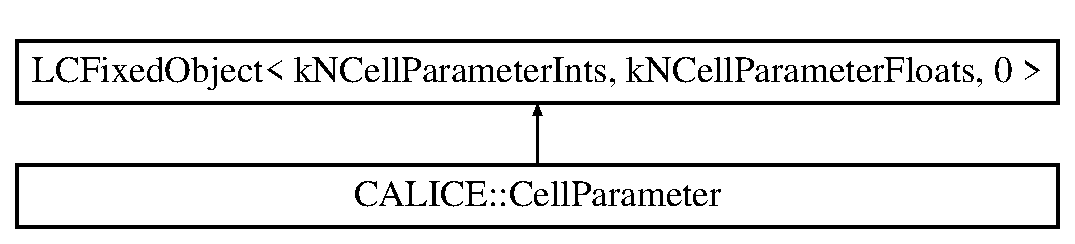
\includegraphics[height=2.000000cm]{classCALICE_1_1CellParameter}
\end{center}
\end{figure}
\subsection*{Public Member Functions}
\begin{DoxyCompactItemize}
\item 
{\bf Cell\-Parameter} (L\-C\-Object $\ast$obj)\label{classCALICE_1_1CellParameter_a3dbf58dc25acfd28b79bde1793d97cbe}

\begin{DoxyCompactList}\small\item\em 'Copy constructor' needed to interpret L\-C\-Collection read from file/database. \end{DoxyCompactList}\item 
void {\bf reset\-Sums} ()
\begin{DoxyCompactList}\small\item\em Reset the sums which are used to calculate the pedestals and the noise. \end{DoxyCompactList}\item 
void {\bfseries reset\-Saturation\-Counter} ()\label{classCALICE_1_1CellParameter_a899306ee8d7c50c7b4f674826384088f}

\item 
void {\bfseries reset\-Hit\-Counter} ()\label{classCALICE_1_1CellParameter_a96068c40f7efdc6f8065998405f00ca3}

\item 
void {\bfseries reset\-All} ()\label{classCALICE_1_1CellParameter_ac296a0d601c33323999152ee709a1abf}

\item 
void {\bf set\-Sum} (Float\-\_\-t a\-\_\-sum)
\begin{DoxyCompactList}\small\item\em Set the sum of the adc values (used to calculate the pedestal). \end{DoxyCompactList}\item 
Float\-\_\-t {\bf get\-Sum} () const 
\begin{DoxyCompactList}\small\item\em Get the sum of the adc values (used to calculate the pedestal). \end{DoxyCompactList}\item 
void {\bf set\-Sum2} (Float\-\_\-t a\-\_\-sum2)
\begin{DoxyCompactList}\small\item\em Set the sum of the adc values squared (used to calculate the noise). \end{DoxyCompactList}\item 
Float\-\_\-t {\bf get\-Sum2} () const 
\begin{DoxyCompactList}\small\item\em Get the sum of the adc values squared (used to calculate the noise). \end{DoxyCompactList}\item 
void {\bf set\-N\-Values} (U\-Int\-\_\-t n\-\_\-values)\label{classCALICE_1_1CellParameter_acd7683bda27b9dc1a3b9bf9dd67fdc69}

\begin{DoxyCompactList}\small\item\em Set the number of values added to the sums. \end{DoxyCompactList}\item 
U\-Int\-\_\-t {\bf get\-N\-Values} () const \label{classCALICE_1_1CellParameter_a9d83d4f709324d0bbdd464c54aa1a39c}

\begin{DoxyCompactList}\small\item\em Get the number of values added to the sums. \end{DoxyCompactList}\item 
void {\bf set\-Pedestal} (Float\-\_\-t a\-\_\-pedestal)\label{classCALICE_1_1CellParameter_af3c9c24f740b0822c4b996a363507cf5}

\begin{DoxyCompactList}\small\item\em Set the pedestal. \end{DoxyCompactList}\item 
Float\-\_\-t {\bf get\-Pedestal} () const 
\begin{DoxyCompactList}\small\item\em Get the pedestal. \end{DoxyCompactList}\item 
void {\bf set\-Old\-Pedestal} (Float\-\_\-t an\-\_\-old\-\_\-pedestal)
\begin{DoxyCompactList}\small\item\em Set the old pedestal. \end{DoxyCompactList}\item 
Float\-\_\-t {\bf get\-Old\-Pedestal} () const 
\begin{DoxyCompactList}\small\item\em Get the old pedestal The result is undefined before the pedestals and the noise have been adjusted or calculated. \end{DoxyCompactList}\item 
void {\bf set\-Noise} (Float\-\_\-t a\-\_\-noise)\label{classCALICE_1_1CellParameter_a4ecc22743f2049d0558d6d625038907d}

\begin{DoxyCompactList}\small\item\em Set the noise. \end{DoxyCompactList}\item 
Float\-\_\-t {\bf get\-Noise} () const 
\begin{DoxyCompactList}\small\item\em Get the noise. \end{DoxyCompactList}\item 
void {\bf set\-Old\-Noise} (Float\-\_\-t an\-\_\-old\-\_\-noise)
\begin{DoxyCompactList}\small\item\em Set the old noise. \end{DoxyCompactList}\item 
Float\-\_\-t {\bf get\-Old\-Noise} () const 
\begin{DoxyCompactList}\small\item\em Get the old noise. \end{DoxyCompactList}\item 
void {\bf set\-Max\-Value} (Float\-\_\-t a\-\_\-max\-\_\-value)
\begin{DoxyCompactList}\small\item\em set the maximum value for a cell ({\bfseries shares storage with pedestal}). \end{DoxyCompactList}\item 
Float\-\_\-t {\bf get\-Max\-Value} () const \label{classCALICE_1_1CellParameter_af1a12f740874cc83f5e35ba5d8d0eefd}

\begin{DoxyCompactList}\small\item\em get the maximum value of a cell (shares storage with pedestal) This function only returns the expected result before pedestals/noise are calculated. \end{DoxyCompactList}\item 
void {\bf add} (Float\-\_\-t adc)
\begin{DoxyCompactList}\small\item\em Build sums used to calculate pedestals and noise. \end{DoxyCompactList}\item 
void {\bf sub} (Float\-\_\-t adc)
\begin{DoxyCompactList}\small\item\em Subtract a previously added adc value from the sums to return to the prior condition. \end{DoxyCompactList}\item 
void {\bf calculate} ()\label{classCALICE_1_1CellParameter_a0548e12eab1fdba4da79dee09bc18aee}

\begin{DoxyCompactList}\small\item\em Caluclate the pedestal and the noise from the sums. \end{DoxyCompactList}\item 
void {\bf adjust\-Pedestal\-Noise} (Float\-\_\-t adc, U\-Int\-\_\-t keep\-\_\-n\-\_\-minus\-\_\-one)
\begin{DoxyCompactList}\small\item\em Adjust the pedestal and the noise using the new A\-D\-C value. \end{DoxyCompactList}\item 
Bool\-\_\-t {\bf is\-Dead} () const \label{classCALICE_1_1CellParameter_ab1ae07641b9b6d188cfc8aa7b6641e0a}

\begin{DoxyCompactList}\small\item\em Return k\-T\-R\-U\-E if the pad is considered to be dead. \end{DoxyCompactList}\item 
void {\bf set\-Dead} (Bool\-\_\-t is\-\_\-dead=true)
\begin{DoxyCompactList}\small\item\em Declare the pad to be dead (or revive pad (is\-\_\-dead=k\-F\-A\-L\-S\-E). \end{DoxyCompactList}\item 
U\-Int\-\_\-t {\bf get\-Saturation\-Counter} () const 
\begin{DoxyCompactList}\small\item\em Get the value of the saturation counter. \end{DoxyCompactList}\item 
void {\bf increment\-Saturation\-Counter} ()
\begin{DoxyCompactList}\small\item\em Increment the saturation counter. \end{DoxyCompactList}\item 
U\-Int\-\_\-t {\bf get\-N\-Hits} () const 
\begin{DoxyCompactList}\small\item\em Get the number of hits. \end{DoxyCompactList}\item 
void {\bf increment\-N\-Hits} ()
\begin{DoxyCompactList}\small\item\em Increment the hit counter. \end{DoxyCompactList}\item 
Float\-\_\-t {\bf get\-N\-Hits\-Float} () const 
\begin{DoxyCompactList}\small\item\em Function which returns the number of hits converted into a float. \end{DoxyCompactList}\item 
void {\bf init\-A\-D\-C\-Memory} ()
\begin{DoxyCompactList}\small\item\em Initialse the array which memorises the last pedestal subtracted values. \end{DoxyCompactList}\item 
void {\bf set\-A\-D\-C\-Memory\-Value} (U\-Int\-\_\-t memory\-\_\-cell\-\_\-i, Float\-\_\-t an\-\_\-adc\-\_\-value)\label{classCALICE_1_1CellParameter_a2150862e4495b17184abcad51b85d67d}

\begin{DoxyCompactList}\small\item\em Memorise an A\-D\-C value in the given cell. \end{DoxyCompactList}\item 
Float\-\_\-t {\bf get\-A\-D\-C\-Memory\-Value} (U\-Int\-\_\-t memory\-\_\-cell\-\_\-i) const \label{classCALICE_1_1CellParameter_a64123c38f4b0fb4e0c519d2c144d89db}

\begin{DoxyCompactList}\small\item\em Get a memorised A\-D\-C value from the given cell. \end{DoxyCompactList}\item 
void {\bf set\-A\-D\-C\-Memory\-Write\-Pos} (U\-Int\-\_\-t memory\-\_\-cell\-\_\-i)\label{classCALICE_1_1CellParameter_a6d667e7086d288b9797ea58407ab6eba}

\begin{DoxyCompactList}\small\item\em Set the current A\-D\-C memory cell. \end{DoxyCompactList}\item 
void {\bfseries set\-Next\-A\-D\-C\-Memory} ()\label{classCALICE_1_1CellParameter_acd3539f67f1b47ebdd719e0393788b94}

\item 
Float\-\_\-t {\bf get\-A\-D\-C\-Memory\-Value} () const \label{classCALICE_1_1CellParameter_a6d46c4d193e8d3bda70f0f6f8a350ef9}

\begin{DoxyCompactList}\small\item\em Get a memorised A\-D\-C value. \end{DoxyCompactList}\item 
void {\bf set\-A\-D\-C\-Memory\-Value} (Float\-\_\-t pedestal\-\_\-subtracted\-\_\-value)
\begin{DoxyCompactList}\small\item\em Memorise an A\-D\-C value. \end{DoxyCompactList}\item 
Float\-\_\-t {\bf get\-Mean\-A\-D\-C\-Value} (Float\-\_\-t pedestal\-\_\-subtracted\-\_\-value)
\begin{DoxyCompactList}\small\item\em Get the mean value of a group of pedestal subtracted A\-D\-C values (the maximum is removed). \end{DoxyCompactList}\item 
void {\bf shift\-Pedestal} (Float\-\_\-t shift)
\begin{DoxyCompactList}\small\item\em Shift the current and the old pedestal by this value. \end{DoxyCompactList}\item 
U\-Int\-\_\-t {\bf get\-N\-Pedestal\-Changes} () const 
\begin{DoxyCompactList}\small\item\em Get the value of the pedestal change counter. \end{DoxyCompactList}\item 
const std\-::string {\bf get\-Type\-Name} () const \label{classCALICE_1_1CellParameter_add6643930ab5dcb3ff15c8a0aeeb65a4}

\begin{DoxyCompactList}\small\item\em Return the type of the class. \end{DoxyCompactList}\item 
const std\-::string {\bf get\-Data\-Description} () const \label{classCALICE_1_1CellParameter_a510675057c37ce93c7f992257c9cc8bb}

\begin{DoxyCompactList}\small\item\em Return a brief description of the data members. \end{DoxyCompactList}\end{DoxyCompactItemize}
\subsection*{Protected Member Functions}
\begin{DoxyCompactItemize}
\item 
void {\bf set\-Saturation\-Counter} (U\-Int\-\_\-t saturation)
\begin{DoxyCompactList}\small\item\em Set the value of the saturation counter. \end{DoxyCompactList}\item 
void {\bf set\-N\-Hits} (U\-Int\-\_\-t n\-\_\-hits)
\begin{DoxyCompactList}\small\item\em Set the value of the hit counter. \end{DoxyCompactList}\item 
void {\bf set\-N\-Pedestal\-Changes} (U\-Int\-\_\-t n\-\_\-pedestal\-\_\-changes)
\begin{DoxyCompactList}\small\item\em Set the value of the pedestal change counter. \end{DoxyCompactList}\item 
void {\bf increment\-N\-Pedestal\-Changes} ()
\begin{DoxyCompactList}\small\item\em Increment the pedestal change counter. \end{DoxyCompactList}\end{DoxyCompactItemize}


\subsection{Detailed Description}
Information about a pad\-: Pedestal, noise, etc. 

This class hold the pedestal, the noise, the number of accumulated hits, a saturation counter and a flag which indicates whether the pad is considered to be dead. 

Definition at line 70 of file Cell\-Parameter.\-hh.



\subsection{Member Function Documentation}
\index{C\-A\-L\-I\-C\-E\-::\-Cell\-Parameter@{C\-A\-L\-I\-C\-E\-::\-Cell\-Parameter}!add@{add}}
\index{add@{add}!CALICE::CellParameter@{C\-A\-L\-I\-C\-E\-::\-Cell\-Parameter}}
\subsubsection[{add}]{\setlength{\rightskip}{0pt plus 5cm}void C\-A\-L\-I\-C\-E\-::\-Cell\-Parameter\-::add (
\begin{DoxyParamCaption}
\item[{Float\-\_\-t}]{adc}
\end{DoxyParamCaption}
)\hspace{0.3cm}{\ttfamily [inline]}}\label{classCALICE_1_1CellParameter_a199f221d2988995dedbb75b9be43e9ab}


Build sums used to calculate pedestals and noise. 

The storage for the old pedestals and noise is abused to store the sums \begin{DoxySeeAlso}{See Also}
\doxyref{Cell\-Parameter\-::sub}{p.}{classCALICE_1_1CellParameter_a09cb9e322c9b22d1591244eaa1ded505} 
\end{DoxySeeAlso}


Definition at line 190 of file Cell\-Parameter.\-hh.



Referenced by C\-A\-L\-I\-C\-E\-::\-Simple\-Hit\-Search\-::accumulate\-Events\-For\-Initial\-Pedestal\-Noise\-Calculation(), C\-A\-L\-I\-C\-E\-::\-Simple\-Hit\-Search\-::accumulate\-Events\-For\-Pedestal\-Noise\-Calculation\-With\-Hit\-Rejection(), and C\-A\-L\-I\-C\-E\-::\-Simple\-Hit\-Search\-::accumulate\-Events\-For\-Pedestal\-Noise\-Calculation\-With\-Hit\-Rejection\-And\-Pedestal\-Shift\-Detection().

\index{C\-A\-L\-I\-C\-E\-::\-Cell\-Parameter@{C\-A\-L\-I\-C\-E\-::\-Cell\-Parameter}!adjust\-Pedestal\-Noise@{adjust\-Pedestal\-Noise}}
\index{adjust\-Pedestal\-Noise@{adjust\-Pedestal\-Noise}!CALICE::CellParameter@{C\-A\-L\-I\-C\-E\-::\-Cell\-Parameter}}
\subsubsection[{adjust\-Pedestal\-Noise}]{\setlength{\rightskip}{0pt plus 5cm}void C\-A\-L\-I\-C\-E\-::\-Cell\-Parameter\-::adjust\-Pedestal\-Noise (
\begin{DoxyParamCaption}
\item[{Float\-\_\-t}]{adc, }
\item[{U\-Int\-\_\-t}]{keep\-\_\-n\-\_\-minus\-\_\-one}
\end{DoxyParamCaption}
)\hspace{0.3cm}{\ttfamily [inline]}}\label{classCALICE_1_1CellParameter_a15bfbaa4918ac7d9aaf841c0483a8a19}


Adjust the pedestal and the noise using the new A\-D\-C value. 


\begin{DoxyParams}{Parameters}
{\em adc} & the new A\-D\-C value \\
\hline
{\em keep\-\_\-n\-\_\-minus\-\_\-one} & the current pedestal and noise are given a weight of this value + 1 and the new A\-D\-C value get the weight 1\\
\hline
\end{DoxyParams}
The current pedestal and the current noise are memorised (\doxyref{get\-Pedestal}{p.}{classCALICE_1_1CellParameter_a3223608e5f680b674e7181b5c4495935} and \doxyref{get\-Noise}{p.}{classCALICE_1_1CellParameter_a58d1f99e4ef0452b94fef27d5de1cc1e}) and then they are updated. 

Definition at line 230 of file Cell\-Parameter.\-hh.



References get\-Noise(), get\-Pedestal(), set\-Noise(), set\-Old\-Noise(), set\-Old\-Pedestal(), and set\-Pedestal().



Referenced by C\-A\-L\-I\-C\-E\-::\-Simple\-Hit\-Search\-::search\-Hits\-And\-Adjust\-Pedestals\-And\-Noise().

\index{C\-A\-L\-I\-C\-E\-::\-Cell\-Parameter@{C\-A\-L\-I\-C\-E\-::\-Cell\-Parameter}!get\-Mean\-A\-D\-C\-Value@{get\-Mean\-A\-D\-C\-Value}}
\index{get\-Mean\-A\-D\-C\-Value@{get\-Mean\-A\-D\-C\-Value}!CALICE::CellParameter@{C\-A\-L\-I\-C\-E\-::\-Cell\-Parameter}}
\subsubsection[{get\-Mean\-A\-D\-C\-Value}]{\setlength{\rightskip}{0pt plus 5cm}Float\-\_\-t C\-A\-L\-I\-C\-E\-::\-Cell\-Parameter\-::get\-Mean\-A\-D\-C\-Value (
\begin{DoxyParamCaption}
\item[{Float\-\_\-t}]{pedestal\-\_\-subtracted\-\_\-value}
\end{DoxyParamCaption}
)\hspace{0.3cm}{\ttfamily [inline]}}\label{classCALICE_1_1CellParameter_a70a20f2d63910738f6d725fd5db83d4f}


Get the mean value of a group of pedestal subtracted A\-D\-C values (the maximum is removed). 

The mean value is used to track jumps in the pedestal. If the jump is larger than a certain threshold the pedestal is considered to have changed. 

Definition at line 387 of file Cell\-Parameter.\-hh.



References get\-A\-D\-C\-Memory\-Value(), and set\-A\-D\-C\-Memory\-Value().



Referenced by C\-A\-L\-I\-C\-E\-::\-Simple\-Hit\-Search\-::accumulate\-Events\-For\-Pedestal\-Noise\-Calculation\-With\-Hit\-Rejection\-And\-Pedestal\-Shift\-Detection().

\index{C\-A\-L\-I\-C\-E\-::\-Cell\-Parameter@{C\-A\-L\-I\-C\-E\-::\-Cell\-Parameter}!get\-N\-Hits@{get\-N\-Hits}}
\index{get\-N\-Hits@{get\-N\-Hits}!CALICE::CellParameter@{C\-A\-L\-I\-C\-E\-::\-Cell\-Parameter}}
\subsubsection[{get\-N\-Hits}]{\setlength{\rightskip}{0pt plus 5cm}U\-Int\-\_\-t C\-A\-L\-I\-C\-E\-::\-Cell\-Parameter\-::get\-N\-Hits (
\begin{DoxyParamCaption}
{}
\end{DoxyParamCaption}
) const\hspace{0.3cm}{\ttfamily [inline]}}\label{classCALICE_1_1CellParameter_aaeb9e38b31539b337be9e7b0522005ef}


Get the number of hits. 

The hit counter is increased when ever the pedestal subtracted A\-D\-C value is above a signal or signal-\/to-\/noise threshold. 

Definition at line 291 of file Cell\-Parameter.\-hh.



Referenced by get\-N\-Hits\-Float(), and increment\-N\-Hits().

\index{C\-A\-L\-I\-C\-E\-::\-Cell\-Parameter@{C\-A\-L\-I\-C\-E\-::\-Cell\-Parameter}!get\-N\-Hits\-Float@{get\-N\-Hits\-Float}}
\index{get\-N\-Hits\-Float@{get\-N\-Hits\-Float}!CALICE::CellParameter@{C\-A\-L\-I\-C\-E\-::\-Cell\-Parameter}}
\subsubsection[{get\-N\-Hits\-Float}]{\setlength{\rightskip}{0pt plus 5cm}Float\-\_\-t C\-A\-L\-I\-C\-E\-::\-Cell\-Parameter\-::get\-N\-Hits\-Float (
\begin{DoxyParamCaption}
{}
\end{DoxyParamCaption}
) const\hspace{0.3cm}{\ttfamily [inline]}}\label{classCALICE_1_1CellParameter_a32aaee7ca8e819dae916272e109171f5}


Function which returns the number of hits converted into a float. 

This function can be used together with get\-Noise and get\-Pedestal in a generic way (e.\-g. typedef Float\-\_\-t \doxyref{Cell\-Parameter}{p.}{classCALICE_1_1CellParameter}\-:\-:$\ast$\-Get\-Float\-Func\-\_\-t();) 

Definition at line 302 of file Cell\-Parameter.\-hh.



References get\-N\-Hits().

\index{C\-A\-L\-I\-C\-E\-::\-Cell\-Parameter@{C\-A\-L\-I\-C\-E\-::\-Cell\-Parameter}!get\-Noise@{get\-Noise}}
\index{get\-Noise@{get\-Noise}!CALICE::CellParameter@{C\-A\-L\-I\-C\-E\-::\-Cell\-Parameter}}
\subsubsection[{get\-Noise}]{\setlength{\rightskip}{0pt plus 5cm}Float\-\_\-t C\-A\-L\-I\-C\-E\-::\-Cell\-Parameter\-::get\-Noise (
\begin{DoxyParamCaption}
{}
\end{DoxyParamCaption}
) const\hspace{0.3cm}{\ttfamily [inline]}}\label{classCALICE_1_1CellParameter_a58d1f99e4ef0452b94fef27d5de1cc1e}


Get the noise. 

The result is undefined before the pedestals and the noise are calculated. 

Definition at line 153 of file Cell\-Parameter.\-hh.



Referenced by C\-A\-L\-I\-C\-E\-::\-Simple\-Hit\-Search\-::accumulate\-Events\-For\-Pedestal\-Noise\-Calculation\-With\-Hit\-Rejection(), C\-A\-L\-I\-C\-E\-::\-Simple\-Hit\-Search\-::accumulate\-Events\-For\-Pedestal\-Noise\-Calculation\-With\-Hit\-Rejection\-And\-Pedestal\-Shift\-Detection(), adjust\-Pedestal\-Noise(), C\-A\-L\-I\-C\-E\-::\-Simple\-Hit\-Search\-::calculate\-Pedestal\-Noise\-And\-Declare\-Cells\-Dead(), C\-A\-L\-I\-C\-E\-::\-Pedestal\-Noise\-Histograms\-::process\-Event(), C\-A\-L\-I\-C\-E\-::\-Average\-History\-Graphs\-::process\-Event(), C\-A\-L\-I\-C\-E\-::\-Simple\-Hit\-Search\-::search\-Hits(), C\-A\-L\-I\-C\-E\-::\-Simple\-Hit\-Search\-::search\-Hits\-And\-Adjust\-Pedestals\-And\-Noise(), and C\-A\-L\-I\-C\-E\-::\-Simple\-Hit\-Search\-::show\-Noise\-Stat().

\index{C\-A\-L\-I\-C\-E\-::\-Cell\-Parameter@{C\-A\-L\-I\-C\-E\-::\-Cell\-Parameter}!get\-N\-Pedestal\-Changes@{get\-N\-Pedestal\-Changes}}
\index{get\-N\-Pedestal\-Changes@{get\-N\-Pedestal\-Changes}!CALICE::CellParameter@{C\-A\-L\-I\-C\-E\-::\-Cell\-Parameter}}
\subsubsection[{get\-N\-Pedestal\-Changes}]{\setlength{\rightskip}{0pt plus 5cm}U\-Int\-\_\-t C\-A\-L\-I\-C\-E\-::\-Cell\-Parameter\-::get\-N\-Pedestal\-Changes (
\begin{DoxyParamCaption}
{}
\end{DoxyParamCaption}
) const\hspace{0.3cm}{\ttfamily [inline]}}\label{classCALICE_1_1CellParameter_a8f6f313321e39c27dc7f09899aa6e948}


Get the value of the pedestal change counter. 

The Pedestal\-Change counter is increased when ever the A\-D\-C value is outside of a certain range 

Definition at line 425 of file Cell\-Parameter.\-hh.



Referenced by increment\-N\-Pedestal\-Changes().

\index{C\-A\-L\-I\-C\-E\-::\-Cell\-Parameter@{C\-A\-L\-I\-C\-E\-::\-Cell\-Parameter}!get\-Old\-Noise@{get\-Old\-Noise}}
\index{get\-Old\-Noise@{get\-Old\-Noise}!CALICE::CellParameter@{C\-A\-L\-I\-C\-E\-::\-Cell\-Parameter}}
\subsubsection[{get\-Old\-Noise}]{\setlength{\rightskip}{0pt plus 5cm}Float\-\_\-t C\-A\-L\-I\-C\-E\-::\-Cell\-Parameter\-::get\-Old\-Noise (
\begin{DoxyParamCaption}
{}
\end{DoxyParamCaption}
) const\hspace{0.3cm}{\ttfamily [inline]}}\label{classCALICE_1_1CellParameter_a3bfb3c568c64aee79f779c649b941dc7}


Get the old noise. 

The result is undefined before the pedestals and the noise have been adjusted or calculated. In the latter case the old and the \char`\"{}new\char`\"{} noise are the same. 

Definition at line 164 of file Cell\-Parameter.\-hh.



Referenced by C\-A\-L\-I\-C\-E\-::\-Simple\-Hit\-Search\-::search\-Hits\-And\-Adjust\-Pedestals\-And\-Noise(), and C\-A\-L\-I\-C\-E\-::\-Simple\-Hit\-Search\-::show\-Current\-Noise\-Stat().

\index{C\-A\-L\-I\-C\-E\-::\-Cell\-Parameter@{C\-A\-L\-I\-C\-E\-::\-Cell\-Parameter}!get\-Old\-Pedestal@{get\-Old\-Pedestal}}
\index{get\-Old\-Pedestal@{get\-Old\-Pedestal}!CALICE::CellParameter@{C\-A\-L\-I\-C\-E\-::\-Cell\-Parameter}}
\subsubsection[{get\-Old\-Pedestal}]{\setlength{\rightskip}{0pt plus 5cm}Float\-\_\-t C\-A\-L\-I\-C\-E\-::\-Cell\-Parameter\-::get\-Old\-Pedestal (
\begin{DoxyParamCaption}
{}
\end{DoxyParamCaption}
) const\hspace{0.3cm}{\ttfamily [inline]}}\label{classCALICE_1_1CellParameter_ac159d4054fd122bfb2fb6c6730110126}


Get the old pedestal The result is undefined before the pedestals and the noise have been adjusted or calculated. 

In the latter case the old and the \char`\"{}new\char`\"{} pedestals are the same. 

Definition at line 143 of file Cell\-Parameter.\-hh.



Referenced by C\-A\-L\-I\-C\-E\-::\-Simple\-Hit\-Search\-::search\-Hits\-And\-Adjust\-Pedestals\-And\-Noise(), shift\-Pedestal(), and C\-A\-L\-I\-C\-E\-::\-Simple\-Hit\-Search\-::show\-Current\-Noise\-Stat().

\index{C\-A\-L\-I\-C\-E\-::\-Cell\-Parameter@{C\-A\-L\-I\-C\-E\-::\-Cell\-Parameter}!get\-Pedestal@{get\-Pedestal}}
\index{get\-Pedestal@{get\-Pedestal}!CALICE::CellParameter@{C\-A\-L\-I\-C\-E\-::\-Cell\-Parameter}}
\subsubsection[{get\-Pedestal}]{\setlength{\rightskip}{0pt plus 5cm}Float\-\_\-t C\-A\-L\-I\-C\-E\-::\-Cell\-Parameter\-::get\-Pedestal (
\begin{DoxyParamCaption}
{}
\end{DoxyParamCaption}
) const\hspace{0.3cm}{\ttfamily [inline]}}\label{classCALICE_1_1CellParameter_a3223608e5f680b674e7181b5c4495935}


Get the pedestal. 

The result is undefined before the pedestals and the noise are calculated. 

Definition at line 131 of file Cell\-Parameter.\-hh.



Referenced by C\-A\-L\-I\-C\-E\-::\-Simple\-Hit\-Search\-::accumulate\-Events\-For\-Pedestal\-Noise\-Calculation\-With\-Hit\-Rejection(), C\-A\-L\-I\-C\-E\-::\-Simple\-Hit\-Search\-::accumulate\-Events\-For\-Pedestal\-Noise\-Calculation\-With\-Hit\-Rejection\-And\-Pedestal\-Shift\-Detection(), adjust\-Pedestal\-Noise(), C\-A\-L\-I\-C\-E\-::\-Simple\-Hit\-Search\-::calculate\-Pedestal\-Noise\-And\-Declare\-Cells\-Dead(), init\-A\-D\-C\-Memory(), C\-A\-L\-I\-C\-E\-::\-Pedestal\-Noise\-Histograms\-::process\-Event(), C\-A\-L\-I\-C\-E\-::\-Average\-History\-Graphs\-::process\-Event(), C\-A\-L\-I\-C\-E\-::\-Simple\-Hit\-Search\-::search\-Hits(), C\-A\-L\-I\-C\-E\-::\-Simple\-Hit\-Search\-::search\-Hits\-And\-Adjust\-Pedestals\-And\-Noise(), shift\-Pedestal(), and C\-A\-L\-I\-C\-E\-::\-Simple\-Hit\-Search\-::show\-Noise\-Stat().

\index{C\-A\-L\-I\-C\-E\-::\-Cell\-Parameter@{C\-A\-L\-I\-C\-E\-::\-Cell\-Parameter}!get\-Saturation\-Counter@{get\-Saturation\-Counter}}
\index{get\-Saturation\-Counter@{get\-Saturation\-Counter}!CALICE::CellParameter@{C\-A\-L\-I\-C\-E\-::\-Cell\-Parameter}}
\subsubsection[{get\-Saturation\-Counter}]{\setlength{\rightskip}{0pt plus 5cm}U\-Int\-\_\-t C\-A\-L\-I\-C\-E\-::\-Cell\-Parameter\-::get\-Saturation\-Counter (
\begin{DoxyParamCaption}
{}
\end{DoxyParamCaption}
) const\hspace{0.3cm}{\ttfamily [inline]}}\label{classCALICE_1_1CellParameter_ae4ef4a080c6400a667dd37dd7ce853fd}


Get the value of the saturation counter. 

The saturation counter is increased when ever the A\-D\-C value is outside of a certain range. The saturation counter is used to mark cells as dead. Thus, it must not be incremented if a cell is dead. 

Definition at line 274 of file Cell\-Parameter.\-hh.



Referenced by C\-A\-L\-I\-C\-E\-::\-Simple\-Hit\-Search\-::calculate\-Pedestal\-Noise\-And\-Declare\-Cells\-Dead(), increment\-Saturation\-Counter(), and is\-Dead().

\index{C\-A\-L\-I\-C\-E\-::\-Cell\-Parameter@{C\-A\-L\-I\-C\-E\-::\-Cell\-Parameter}!get\-Sum@{get\-Sum}}
\index{get\-Sum@{get\-Sum}!CALICE::CellParameter@{C\-A\-L\-I\-C\-E\-::\-Cell\-Parameter}}
\subsubsection[{get\-Sum}]{\setlength{\rightskip}{0pt plus 5cm}Float\-\_\-t C\-A\-L\-I\-C\-E\-::\-Cell\-Parameter\-::get\-Sum (
\begin{DoxyParamCaption}
{}
\end{DoxyParamCaption}
) const\hspace{0.3cm}{\ttfamily [inline]}}\label{classCALICE_1_1CellParameter_afa7c61c8a0fd6f4b93d5113c2ee30285}


Get the sum of the adc values (used to calculate the pedestal). 

The result is undefined after the noise and the pedestals have been calculated. 

Definition at line 101 of file Cell\-Parameter.\-hh.



Referenced by calculate().

\index{C\-A\-L\-I\-C\-E\-::\-Cell\-Parameter@{C\-A\-L\-I\-C\-E\-::\-Cell\-Parameter}!get\-Sum2@{get\-Sum2}}
\index{get\-Sum2@{get\-Sum2}!CALICE::CellParameter@{C\-A\-L\-I\-C\-E\-::\-Cell\-Parameter}}
\subsubsection[{get\-Sum2}]{\setlength{\rightskip}{0pt plus 5cm}Float\-\_\-t C\-A\-L\-I\-C\-E\-::\-Cell\-Parameter\-::get\-Sum2 (
\begin{DoxyParamCaption}
{}
\end{DoxyParamCaption}
) const\hspace{0.3cm}{\ttfamily [inline]}}\label{classCALICE_1_1CellParameter_ac509a47a088106a0fbd2fc2fc17dcca0}


Get the sum of the adc values squared (used to calculate the noise). 

The result is undefined after the noise and the pedestals have been calculated. 

Definition at line 112 of file Cell\-Parameter.\-hh.



Referenced by calculate().

\index{C\-A\-L\-I\-C\-E\-::\-Cell\-Parameter@{C\-A\-L\-I\-C\-E\-::\-Cell\-Parameter}!increment\-N\-Hits@{increment\-N\-Hits}}
\index{increment\-N\-Hits@{increment\-N\-Hits}!CALICE::CellParameter@{C\-A\-L\-I\-C\-E\-::\-Cell\-Parameter}}
\subsubsection[{increment\-N\-Hits}]{\setlength{\rightskip}{0pt plus 5cm}void C\-A\-L\-I\-C\-E\-::\-Cell\-Parameter\-::increment\-N\-Hits (
\begin{DoxyParamCaption}
{}
\end{DoxyParamCaption}
)\hspace{0.3cm}{\ttfamily [inline]}}\label{classCALICE_1_1CellParameter_ab44ebb0a1c9e33f0fd4dcf7796b6c3de}


Increment the hit counter. 

The hit counter is increased when ever the A\-D\-C value is outside of a certain range 

Definition at line 296 of file Cell\-Parameter.\-hh.



References get\-N\-Hits(), and set\-N\-Hits().



Referenced by C\-A\-L\-I\-C\-E\-::\-Simple\-Hit\-Search\-::search\-Hits(), and C\-A\-L\-I\-C\-E\-::\-Simple\-Hit\-Search\-::search\-Hits\-And\-Adjust\-Pedestals\-And\-Noise().

\index{C\-A\-L\-I\-C\-E\-::\-Cell\-Parameter@{C\-A\-L\-I\-C\-E\-::\-Cell\-Parameter}!increment\-N\-Pedestal\-Changes@{increment\-N\-Pedestal\-Changes}}
\index{increment\-N\-Pedestal\-Changes@{increment\-N\-Pedestal\-Changes}!CALICE::CellParameter@{C\-A\-L\-I\-C\-E\-::\-Cell\-Parameter}}
\subsubsection[{increment\-N\-Pedestal\-Changes}]{\setlength{\rightskip}{0pt plus 5cm}void C\-A\-L\-I\-C\-E\-::\-Cell\-Parameter\-::increment\-N\-Pedestal\-Changes (
\begin{DoxyParamCaption}
{}
\end{DoxyParamCaption}
)\hspace{0.3cm}{\ttfamily [inline]}, {\ttfamily [protected]}}\label{classCALICE_1_1CellParameter_a6c7c08f561c2581f43be8003f2a0312b}


Increment the pedestal change counter. 

The Pedestal\-Change counter is increased when ever the A\-D\-C value is outside of a certain range 

Definition at line 431 of file Cell\-Parameter.\-hh.



References get\-N\-Pedestal\-Changes(), and set\-N\-Pedestal\-Changes().



Referenced by shift\-Pedestal().

\index{C\-A\-L\-I\-C\-E\-::\-Cell\-Parameter@{C\-A\-L\-I\-C\-E\-::\-Cell\-Parameter}!increment\-Saturation\-Counter@{increment\-Saturation\-Counter}}
\index{increment\-Saturation\-Counter@{increment\-Saturation\-Counter}!CALICE::CellParameter@{C\-A\-L\-I\-C\-E\-::\-Cell\-Parameter}}
\subsubsection[{increment\-Saturation\-Counter}]{\setlength{\rightskip}{0pt plus 5cm}void C\-A\-L\-I\-C\-E\-::\-Cell\-Parameter\-::increment\-Saturation\-Counter (
\begin{DoxyParamCaption}
{}
\end{DoxyParamCaption}
)\hspace{0.3cm}{\ttfamily [inline]}}\label{classCALICE_1_1CellParameter_a79423a46a99deb6623624f7974f414b1}


Increment the saturation counter. 

The saturation counter is increased when ever the A\-D\-C value is outside of a certain range 

Definition at line 279 of file Cell\-Parameter.\-hh.



References get\-Saturation\-Counter(), and set\-Saturation\-Counter().



Referenced by C\-A\-L\-I\-C\-E\-::\-Simple\-Hit\-Search\-::accumulate\-Events\-For\-Initial\-Pedestal\-Noise\-Calculation(), C\-A\-L\-I\-C\-E\-::\-Simple\-Hit\-Search\-::accumulate\-Events\-For\-Pedestal\-Noise\-Calculation\-With\-Hit\-Rejection(), C\-A\-L\-I\-C\-E\-::\-Simple\-Hit\-Search\-::accumulate\-Events\-For\-Pedestal\-Noise\-Calculation\-With\-Hit\-Rejection\-And\-Pedestal\-Shift\-Detection(), C\-A\-L\-I\-C\-E\-::\-Simple\-Hit\-Search\-::search\-Hits(), and C\-A\-L\-I\-C\-E\-::\-Simple\-Hit\-Search\-::search\-Hits\-And\-Adjust\-Pedestals\-And\-Noise().

\index{C\-A\-L\-I\-C\-E\-::\-Cell\-Parameter@{C\-A\-L\-I\-C\-E\-::\-Cell\-Parameter}!init\-A\-D\-C\-Memory@{init\-A\-D\-C\-Memory}}
\index{init\-A\-D\-C\-Memory@{init\-A\-D\-C\-Memory}!CALICE::CellParameter@{C\-A\-L\-I\-C\-E\-::\-Cell\-Parameter}}
\subsubsection[{init\-A\-D\-C\-Memory}]{\setlength{\rightskip}{0pt plus 5cm}void C\-A\-L\-I\-C\-E\-::\-Cell\-Parameter\-::init\-A\-D\-C\-Memory (
\begin{DoxyParamCaption}
{}
\end{DoxyParamCaption}
)\hspace{0.3cm}{\ttfamily [inline]}}\label{classCALICE_1_1CellParameter_ad5b4b06d0eb86e98c21d9119fc3a8d30}


Initialse the array which memorises the last pedestal subtracted values. 

\begin{DoxyRefDesc}{Todo}
\item[{\bf Todo}]initialsie with pedestal or zero? \end{DoxyRefDesc}


Definition at line 308 of file Cell\-Parameter.\-hh.



References get\-Pedestal(), and set\-A\-D\-C\-Memory\-Value().

\index{C\-A\-L\-I\-C\-E\-::\-Cell\-Parameter@{C\-A\-L\-I\-C\-E\-::\-Cell\-Parameter}!reset\-Sums@{reset\-Sums}}
\index{reset\-Sums@{reset\-Sums}!CALICE::CellParameter@{C\-A\-L\-I\-C\-E\-::\-Cell\-Parameter}}
\subsubsection[{reset\-Sums}]{\setlength{\rightskip}{0pt plus 5cm}void C\-A\-L\-I\-C\-E\-::\-Cell\-Parameter\-::reset\-Sums (
\begin{DoxyParamCaption}
{}
\end{DoxyParamCaption}
)\hspace{0.3cm}{\ttfamily [inline]}}\label{classCALICE_1_1CellParameter_a6a81bd8e46ad7e4fb8df9847ca4397a5}


Reset the sums which are used to calculate the pedestals and the noise. 

This function should be called before A\-D\-C values are accumulated and added with \doxyref{add}{p.}{classCALICE_1_1CellParameter_a199f221d2988995dedbb75b9be43e9ab} to the sums. 

Definition at line 86 of file Cell\-Parameter.\-hh.



References set\-N\-Values(), set\-Sum(), and set\-Sum2().

\index{C\-A\-L\-I\-C\-E\-::\-Cell\-Parameter@{C\-A\-L\-I\-C\-E\-::\-Cell\-Parameter}!set\-A\-D\-C\-Memory\-Value@{set\-A\-D\-C\-Memory\-Value}}
\index{set\-A\-D\-C\-Memory\-Value@{set\-A\-D\-C\-Memory\-Value}!CALICE::CellParameter@{C\-A\-L\-I\-C\-E\-::\-Cell\-Parameter}}
\subsubsection[{set\-A\-D\-C\-Memory\-Value}]{\setlength{\rightskip}{0pt plus 5cm}void C\-A\-L\-I\-C\-E\-::\-Cell\-Parameter\-::set\-A\-D\-C\-Memory\-Value (
\begin{DoxyParamCaption}
\item[{Float\-\_\-t}]{pedestal\-\_\-subtracted\-\_\-value}
\end{DoxyParamCaption}
)\hspace{0.3cm}{\ttfamily [inline]}}\label{classCALICE_1_1CellParameter_aea4348d37ee17df1cec6c4a2e8c38217}


Memorise an A\-D\-C value. 

The given pedestal subtracted A\-D\-C value is memorised at the current write postion and the position counter is advanced. 

Definition at line 379 of file Cell\-Parameter.\-hh.

\index{C\-A\-L\-I\-C\-E\-::\-Cell\-Parameter@{C\-A\-L\-I\-C\-E\-::\-Cell\-Parameter}!set\-Dead@{set\-Dead}}
\index{set\-Dead@{set\-Dead}!CALICE::CellParameter@{C\-A\-L\-I\-C\-E\-::\-Cell\-Parameter}}
\subsubsection[{set\-Dead}]{\setlength{\rightskip}{0pt plus 5cm}void C\-A\-L\-I\-C\-E\-::\-Cell\-Parameter\-::set\-Dead (
\begin{DoxyParamCaption}
\item[{Bool\-\_\-t}]{is\-\_\-dead = {\ttfamily true}}
\end{DoxyParamCaption}
)\hspace{0.3cm}{\ttfamily [inline]}}\label{classCALICE_1_1CellParameter_a0ad31de9b53fc6ebed4c7be6a53e7a57}


Declare the pad to be dead (or revive pad (is\-\_\-dead=k\-F\-A\-L\-S\-E). 

The status whether a pad is dead is stored in the saturation counter. Thus, a reviving a cell will reset the saturation counter to zero. 

Definition at line 260 of file Cell\-Parameter.\-hh.



References set\-Saturation\-Counter().



Referenced by C\-A\-L\-I\-C\-E\-::\-Simple\-Hit\-Search\-::calculate\-Pedestal\-Noise\-And\-Declare\-Cells\-Dead().

\index{C\-A\-L\-I\-C\-E\-::\-Cell\-Parameter@{C\-A\-L\-I\-C\-E\-::\-Cell\-Parameter}!set\-Max\-Value@{set\-Max\-Value}}
\index{set\-Max\-Value@{set\-Max\-Value}!CALICE::CellParameter@{C\-A\-L\-I\-C\-E\-::\-Cell\-Parameter}}
\subsubsection[{set\-Max\-Value}]{\setlength{\rightskip}{0pt plus 5cm}void C\-A\-L\-I\-C\-E\-::\-Cell\-Parameter\-::set\-Max\-Value (
\begin{DoxyParamCaption}
\item[{Float\-\_\-t}]{a\-\_\-max\-\_\-value}
\end{DoxyParamCaption}
)\hspace{0.3cm}{\ttfamily [inline]}}\label{classCALICE_1_1CellParameter_add7570a3502df326aa422603be276c8a}


set the maximum value for a cell ({\bfseries shares storage with pedestal}). 

The maximum value is stored in the same place as the pedestal. Thus, the maximum value can only be used during the initial accumulation of pedestal/noise statistics.

k\-Cell\-Parameter\-Float\-Max\-Value and k\-Cell\-Parameter\-Float\-Pedestal point to the same cell 

Definition at line 174 of file Cell\-Parameter.\-hh.



Referenced by C\-A\-L\-I\-C\-E\-::\-Simple\-Hit\-Search\-::accumulate\-Events\-For\-Initial\-Pedestal\-Noise\-Calculation().

\index{C\-A\-L\-I\-C\-E\-::\-Cell\-Parameter@{C\-A\-L\-I\-C\-E\-::\-Cell\-Parameter}!set\-N\-Hits@{set\-N\-Hits}}
\index{set\-N\-Hits@{set\-N\-Hits}!CALICE::CellParameter@{C\-A\-L\-I\-C\-E\-::\-Cell\-Parameter}}
\subsubsection[{set\-N\-Hits}]{\setlength{\rightskip}{0pt plus 5cm}void C\-A\-L\-I\-C\-E\-::\-Cell\-Parameter\-::set\-N\-Hits (
\begin{DoxyParamCaption}
\item[{U\-Int\-\_\-t}]{n\-\_\-hits}
\end{DoxyParamCaption}
)\hspace{0.3cm}{\ttfamily [inline]}, {\ttfamily [protected]}}\label{classCALICE_1_1CellParameter_aefdf93e60fbead8bd62d09ef11f3d540}


Set the value of the hit counter. 

The hit counter is increased when ever the pedestal subtracted A\-D\-C value is above a signal or signal-\/to-\/noise threshold. 

Definition at line 285 of file Cell\-Parameter.\-hh.



Referenced by increment\-N\-Hits().

\index{C\-A\-L\-I\-C\-E\-::\-Cell\-Parameter@{C\-A\-L\-I\-C\-E\-::\-Cell\-Parameter}!set\-N\-Pedestal\-Changes@{set\-N\-Pedestal\-Changes}}
\index{set\-N\-Pedestal\-Changes@{set\-N\-Pedestal\-Changes}!CALICE::CellParameter@{C\-A\-L\-I\-C\-E\-::\-Cell\-Parameter}}
\subsubsection[{set\-N\-Pedestal\-Changes}]{\setlength{\rightskip}{0pt plus 5cm}void C\-A\-L\-I\-C\-E\-::\-Cell\-Parameter\-::set\-N\-Pedestal\-Changes (
\begin{DoxyParamCaption}
\item[{U\-Int\-\_\-t}]{n\-\_\-pedestal\-\_\-changes}
\end{DoxyParamCaption}
)\hspace{0.3cm}{\ttfamily [inline]}, {\ttfamily [protected]}}\label{classCALICE_1_1CellParameter_a1980533fe8a284bed40839d8a9fcf523}


Set the value of the pedestal change counter. 

The Pedestal\-Change counter is increased when ever the A\-D\-C value is outside of a certain range 

Definition at line 419 of file Cell\-Parameter.\-hh.



Referenced by increment\-N\-Pedestal\-Changes().

\index{C\-A\-L\-I\-C\-E\-::\-Cell\-Parameter@{C\-A\-L\-I\-C\-E\-::\-Cell\-Parameter}!set\-Old\-Noise@{set\-Old\-Noise}}
\index{set\-Old\-Noise@{set\-Old\-Noise}!CALICE::CellParameter@{C\-A\-L\-I\-C\-E\-::\-Cell\-Parameter}}
\subsubsection[{set\-Old\-Noise}]{\setlength{\rightskip}{0pt plus 5cm}void C\-A\-L\-I\-C\-E\-::\-Cell\-Parameter\-::set\-Old\-Noise (
\begin{DoxyParamCaption}
\item[{Float\-\_\-t}]{an\-\_\-old\-\_\-noise}
\end{DoxyParamCaption}
)\hspace{0.3cm}{\ttfamily [inline]}}\label{classCALICE_1_1CellParameter_a2b4a500e8cd39fda7dc51ec89d2b0b81}


Set the old noise. 

The old noise shares the storage with the sum2. Thus, after this call the sum2 is invalid. 

Definition at line 158 of file Cell\-Parameter.\-hh.



Referenced by adjust\-Pedestal\-Noise(), and calculate().

\index{C\-A\-L\-I\-C\-E\-::\-Cell\-Parameter@{C\-A\-L\-I\-C\-E\-::\-Cell\-Parameter}!set\-Old\-Pedestal@{set\-Old\-Pedestal}}
\index{set\-Old\-Pedestal@{set\-Old\-Pedestal}!CALICE::CellParameter@{C\-A\-L\-I\-C\-E\-::\-Cell\-Parameter}}
\subsubsection[{set\-Old\-Pedestal}]{\setlength{\rightskip}{0pt plus 5cm}void C\-A\-L\-I\-C\-E\-::\-Cell\-Parameter\-::set\-Old\-Pedestal (
\begin{DoxyParamCaption}
\item[{Float\-\_\-t}]{an\-\_\-old\-\_\-pedestal}
\end{DoxyParamCaption}
)\hspace{0.3cm}{\ttfamily [inline]}}\label{classCALICE_1_1CellParameter_a971b60a79e06210ddc52c25dbf765925}


Set the old pedestal. 

The old pedestal shares the storage with the sum. Thus, after this call the sum is invalid. 

Definition at line 137 of file Cell\-Parameter.\-hh.



Referenced by adjust\-Pedestal\-Noise(), calculate(), C\-A\-L\-I\-C\-E\-::\-Simple\-Hit\-Search\-::search\-Hits(), and shift\-Pedestal().

\index{C\-A\-L\-I\-C\-E\-::\-Cell\-Parameter@{C\-A\-L\-I\-C\-E\-::\-Cell\-Parameter}!set\-Saturation\-Counter@{set\-Saturation\-Counter}}
\index{set\-Saturation\-Counter@{set\-Saturation\-Counter}!CALICE::CellParameter@{C\-A\-L\-I\-C\-E\-::\-Cell\-Parameter}}
\subsubsection[{set\-Saturation\-Counter}]{\setlength{\rightskip}{0pt plus 5cm}void C\-A\-L\-I\-C\-E\-::\-Cell\-Parameter\-::set\-Saturation\-Counter (
\begin{DoxyParamCaption}
\item[{U\-Int\-\_\-t}]{saturation}
\end{DoxyParamCaption}
)\hspace{0.3cm}{\ttfamily [inline]}, {\ttfamily [protected]}}\label{classCALICE_1_1CellParameter_a0ca243bcfe86c85a767ac69082667a5f}


Set the value of the saturation counter. 

The saturation counter is increased when ever the A\-D\-C value is outside of a certain range 

Definition at line 266 of file Cell\-Parameter.\-hh.



Referenced by increment\-Saturation\-Counter(), and set\-Dead().

\index{C\-A\-L\-I\-C\-E\-::\-Cell\-Parameter@{C\-A\-L\-I\-C\-E\-::\-Cell\-Parameter}!set\-Sum@{set\-Sum}}
\index{set\-Sum@{set\-Sum}!CALICE::CellParameter@{C\-A\-L\-I\-C\-E\-::\-Cell\-Parameter}}
\subsubsection[{set\-Sum}]{\setlength{\rightskip}{0pt plus 5cm}void C\-A\-L\-I\-C\-E\-::\-Cell\-Parameter\-::set\-Sum (
\begin{DoxyParamCaption}
\item[{Float\-\_\-t}]{a\-\_\-sum}
\end{DoxyParamCaption}
)\hspace{0.3cm}{\ttfamily [inline]}}\label{classCALICE_1_1CellParameter_aed3095e5d463fbd47ad6175e130e25c0}


Set the sum of the adc values (used to calculate the pedestal). 

After this call the pedestals and the noise are invalid. 

Definition at line 96 of file Cell\-Parameter.\-hh.



Referenced by reset\-Sums().

\index{C\-A\-L\-I\-C\-E\-::\-Cell\-Parameter@{C\-A\-L\-I\-C\-E\-::\-Cell\-Parameter}!set\-Sum2@{set\-Sum2}}
\index{set\-Sum2@{set\-Sum2}!CALICE::CellParameter@{C\-A\-L\-I\-C\-E\-::\-Cell\-Parameter}}
\subsubsection[{set\-Sum2}]{\setlength{\rightskip}{0pt plus 5cm}void C\-A\-L\-I\-C\-E\-::\-Cell\-Parameter\-::set\-Sum2 (
\begin{DoxyParamCaption}
\item[{Float\-\_\-t}]{a\-\_\-sum2}
\end{DoxyParamCaption}
)\hspace{0.3cm}{\ttfamily [inline]}}\label{classCALICE_1_1CellParameter_ae643aab6a440b41afc6d4190988112d0}


Set the sum of the adc values squared (used to calculate the noise). 

After this call the pedestals and the noise are invalid. 

Definition at line 107 of file Cell\-Parameter.\-hh.



Referenced by reset\-Sums().

\index{C\-A\-L\-I\-C\-E\-::\-Cell\-Parameter@{C\-A\-L\-I\-C\-E\-::\-Cell\-Parameter}!shift\-Pedestal@{shift\-Pedestal}}
\index{shift\-Pedestal@{shift\-Pedestal}!CALICE::CellParameter@{C\-A\-L\-I\-C\-E\-::\-Cell\-Parameter}}
\subsubsection[{shift\-Pedestal}]{\setlength{\rightskip}{0pt plus 5cm}void C\-A\-L\-I\-C\-E\-::\-Cell\-Parameter\-::shift\-Pedestal (
\begin{DoxyParamCaption}
\item[{Float\-\_\-t}]{shift}
\end{DoxyParamCaption}
)\hspace{0.3cm}{\ttfamily [inline]}}\label{classCALICE_1_1CellParameter_ad52d1b70e2f0f27cf29020289da277e5}


Shift the current and the old pedestal by this value. 

The pedestal is shifted when a pedestal jump is detected. 

Definition at line 409 of file Cell\-Parameter.\-hh.



References get\-Old\-Pedestal(), get\-Pedestal(), increment\-N\-Pedestal\-Changes(), set\-Old\-Pedestal(), and set\-Pedestal().



Referenced by C\-A\-L\-I\-C\-E\-::\-Simple\-Hit\-Search\-::accumulate\-Events\-For\-Pedestal\-Noise\-Calculation\-With\-Hit\-Rejection\-And\-Pedestal\-Shift\-Detection().

\index{C\-A\-L\-I\-C\-E\-::\-Cell\-Parameter@{C\-A\-L\-I\-C\-E\-::\-Cell\-Parameter}!sub@{sub}}
\index{sub@{sub}!CALICE::CellParameter@{C\-A\-L\-I\-C\-E\-::\-Cell\-Parameter}}
\subsubsection[{sub}]{\setlength{\rightskip}{0pt plus 5cm}void C\-A\-L\-I\-C\-E\-::\-Cell\-Parameter\-::sub (
\begin{DoxyParamCaption}
\item[{Float\-\_\-t}]{adc}
\end{DoxyParamCaption}
)\hspace{0.3cm}{\ttfamily [inline]}}\label{classCALICE_1_1CellParameter_a09cb9e322c9b22d1591244eaa1ded505}


Subtract a previously added adc value from the sums to return to the prior condition. 

\begin{DoxySeeAlso}{See Also}
\doxyref{Cell\-Parameter\-::add}{p.}{classCALICE_1_1CellParameter_a199f221d2988995dedbb75b9be43e9ab} 
\end{DoxySeeAlso}


Definition at line 199 of file Cell\-Parameter.\-hh.



Referenced by C\-A\-L\-I\-C\-E\-::\-Simple\-Hit\-Search\-::accumulate\-Events\-For\-Initial\-Pedestal\-Noise\-Calculation().



The documentation for this class was generated from the following file\-:\begin{DoxyCompactItemize}
\item 
Cell\-Parameter.\-hh\end{DoxyCompactItemize}

\section{C\-A\-L\-I\-C\-E\-:\-:Cell\-Parameter\-Access Class Reference}
\label{classCALICE_1_1CellParameterAccess}\index{C\-A\-L\-I\-C\-E\-::\-Cell\-Parameter\-Access@{C\-A\-L\-I\-C\-E\-::\-Cell\-Parameter\-Access}}


Wrapper around the cell parameter collection to facilitate the access.  




{\ttfamily \#include $<$Cell\-Parameter\-Access.\-hh$>$}

\subsection*{Public Member Functions}
\begin{DoxyCompactItemize}
\item 
{\bf Cell\-Parameter\-Access} (const std\-::string \&col\-\_\-name, E\-V\-E\-N\-T\-::\-L\-C\-Event $\ast$evt\-P)
\begin{DoxyCompactList}\small\item\em Create a simple wrapper to easily access the cell parameters from the L\-C\-Collection. \end{DoxyCompactList}\item 
U\-Int\-\_\-t {\bf get\-Index\-Offset} (U\-Int\-\_\-t module\-\_\-index) const 
\begin{DoxyCompactList}\small\item\em Get the index of the first cell of the given module. \end{DoxyCompactList}\item 
U\-Int\-\_\-t {\bf get\-Index} (U\-Int\-\_\-t module\-\_\-index, U\-Int\-\_\-t cell\-\_\-index) const 
\begin{DoxyCompactList}\small\item\em Get the cell index for the given module and cell index. \end{DoxyCompactList}\item 
{\bf Cell\-Parameter} {\bf get\-Cell\-Parameter} (U\-Int\-\_\-t module\-\_\-index, U\-Int\-\_\-t cell\-\_\-index)
\begin{DoxyCompactList}\small\item\em Get the cell parameters of the specified cell (read/write). \end{DoxyCompactList}\item 
const {\bf Cell\-Parameter} {\bf get\-Cell\-Parameter} (U\-Int\-\_\-t module\-\_\-index, U\-Int\-\_\-t cell\-\_\-index) const 
\begin{DoxyCompactList}\small\item\em Get the cell parameters of the specified cell (read only). \end{DoxyCompactList}\item 
{\bf Cell\-Parameter} {\bf get\-Cell\-Parameter} (U\-Int\-\_\-t index)
\begin{DoxyCompactList}\small\item\em Get the cell parameters of the specified cell (read/write). \end{DoxyCompactList}\item 
const {\bf Cell\-Parameter} {\bf get\-Cell\-Parameter} (U\-Int\-\_\-t index) const 
\begin{DoxyCompactList}\small\item\em Get the cell parameters of the specified cell (read only). \end{DoxyCompactList}\end{DoxyCompactItemize}
\subsection*{Private Attributes}
\begin{DoxyCompactItemize}
\item 
L\-C\-Collection $\ast$ {\bf \-\_\-cell\-Parameter\-Col}\label{classCALICE_1_1CellParameterAccess_a78debadc2027f233e522893ab8132f38}

\begin{DoxyCompactList}\small\item\em The collection of the cell parameters. \end{DoxyCompactList}\item 
Int\-Vec {\bf \-\_\-index\-Offset}
\begin{DoxyCompactList}\small\item\em copy of the array which contains the index offset of the modules. \end{DoxyCompactList}\end{DoxyCompactItemize}


\subsection{Detailed Description}
Wrapper around the cell parameter collection to facilitate the access. 

Definition at line 17 of file Cell\-Parameter\-Access.\-hh.



\subsection{Constructor \& Destructor Documentation}
\index{C\-A\-L\-I\-C\-E\-::\-Cell\-Parameter\-Access@{C\-A\-L\-I\-C\-E\-::\-Cell\-Parameter\-Access}!Cell\-Parameter\-Access@{Cell\-Parameter\-Access}}
\index{Cell\-Parameter\-Access@{Cell\-Parameter\-Access}!CALICE::CellParameterAccess@{C\-A\-L\-I\-C\-E\-::\-Cell\-Parameter\-Access}}
\subsubsection[{Cell\-Parameter\-Access}]{\setlength{\rightskip}{0pt plus 5cm}C\-A\-L\-I\-C\-E\-::\-Cell\-Parameter\-Access\-::\-Cell\-Parameter\-Access (
\begin{DoxyParamCaption}
\item[{const std\-::string \&}]{col\-\_\-name, }
\item[{E\-V\-E\-N\-T\-::\-L\-C\-Event $\ast$}]{evt\-P}
\end{DoxyParamCaption}
)\hspace{0.3cm}{\ttfamily [inline]}}\label{classCALICE_1_1CellParameterAccess_a60d0f03312481332cd43e499bcef974a}


Create a simple wrapper to easily access the cell parameters from the L\-C\-Collection. 


\begin{DoxyExceptions}{Exceptions}
{\em Data\-Not\-Available\-Exception} & if the cell paramter collection does not access. \\
\hline
\end{DoxyExceptions}


Definition at line 23 of file Cell\-Parameter\-Access.\-hh.



References \-\_\-cell\-Parameter\-Col, and \-\_\-index\-Offset.



\subsection{Member Function Documentation}
\index{C\-A\-L\-I\-C\-E\-::\-Cell\-Parameter\-Access@{C\-A\-L\-I\-C\-E\-::\-Cell\-Parameter\-Access}!get\-Cell\-Parameter@{get\-Cell\-Parameter}}
\index{get\-Cell\-Parameter@{get\-Cell\-Parameter}!CALICE::CellParameterAccess@{C\-A\-L\-I\-C\-E\-::\-Cell\-Parameter\-Access}}
\subsubsection[{get\-Cell\-Parameter}]{\setlength{\rightskip}{0pt plus 5cm}{\bf Cell\-Parameter} C\-A\-L\-I\-C\-E\-::\-Cell\-Parameter\-Access\-::get\-Cell\-Parameter (
\begin{DoxyParamCaption}
\item[{U\-Int\-\_\-t}]{module\-\_\-index, }
\item[{U\-Int\-\_\-t}]{cell\-\_\-index}
\end{DoxyParamCaption}
)\hspace{0.3cm}{\ttfamily [inline]}}\label{classCALICE_1_1CellParameterAccess_a9d73c185b55c36fd2ee903246a5dff7d}


Get the cell parameters of the specified cell (read/write). 


\begin{DoxyParams}{Parameters}
{\em module\-\_\-index} & the index of the module (starting from zero). \\
\hline
{\em cell\-\_\-index} & the index of the cell on the specified module (starting from zero). \\
\hline
\end{DoxyParams}
\begin{DoxyReturn}{Returns}
a reference of the cell parameters (read/write access). 
\end{DoxyReturn}


Definition at line 75 of file Cell\-Parameter\-Access.\-hh.



References \-\_\-cell\-Parameter\-Col, and get\-Index().



Referenced by C\-A\-L\-I\-C\-E\-::\-Pedestal\-Noise\-Histograms\-::process\-Event().

\index{C\-A\-L\-I\-C\-E\-::\-Cell\-Parameter\-Access@{C\-A\-L\-I\-C\-E\-::\-Cell\-Parameter\-Access}!get\-Cell\-Parameter@{get\-Cell\-Parameter}}
\index{get\-Cell\-Parameter@{get\-Cell\-Parameter}!CALICE::CellParameterAccess@{C\-A\-L\-I\-C\-E\-::\-Cell\-Parameter\-Access}}
\subsubsection[{get\-Cell\-Parameter}]{\setlength{\rightskip}{0pt plus 5cm}const {\bf Cell\-Parameter} C\-A\-L\-I\-C\-E\-::\-Cell\-Parameter\-Access\-::get\-Cell\-Parameter (
\begin{DoxyParamCaption}
\item[{U\-Int\-\_\-t}]{module\-\_\-index, }
\item[{U\-Int\-\_\-t}]{cell\-\_\-index}
\end{DoxyParamCaption}
) const\hspace{0.3cm}{\ttfamily [inline]}}\label{classCALICE_1_1CellParameterAccess_a519a471698646bf0ae9b59fbd80e7d1f}


Get the cell parameters of the specified cell (read only). 


\begin{DoxyParams}{Parameters}
{\em module\-\_\-index} & the index of the module (starting from zero). \\
\hline
{\em cell\-\_\-index} & the index of the cell on the specified module (starting from zero). \\
\hline
\end{DoxyParams}
\begin{DoxyReturn}{Returns}
a reference of the cell parameters (read only access). 
\end{DoxyReturn}


Definition at line 87 of file Cell\-Parameter\-Access.\-hh.



References \-\_\-cell\-Parameter\-Col, and get\-Index().

\index{C\-A\-L\-I\-C\-E\-::\-Cell\-Parameter\-Access@{C\-A\-L\-I\-C\-E\-::\-Cell\-Parameter\-Access}!get\-Cell\-Parameter@{get\-Cell\-Parameter}}
\index{get\-Cell\-Parameter@{get\-Cell\-Parameter}!CALICE::CellParameterAccess@{C\-A\-L\-I\-C\-E\-::\-Cell\-Parameter\-Access}}
\subsubsection[{get\-Cell\-Parameter}]{\setlength{\rightskip}{0pt plus 5cm}{\bf Cell\-Parameter} C\-A\-L\-I\-C\-E\-::\-Cell\-Parameter\-Access\-::get\-Cell\-Parameter (
\begin{DoxyParamCaption}
\item[{U\-Int\-\_\-t}]{index}
\end{DoxyParamCaption}
)\hspace{0.3cm}{\ttfamily [inline]}}\label{classCALICE_1_1CellParameterAccess_a7df752eebf34fb87ff5be595fbbc1095}


Get the cell parameters of the specified cell (read/write). 


\begin{DoxyParams}{Parameters}
{\em index} & the internal index of the cell (combination of module and cell index). \\
\hline
\end{DoxyParams}
\begin{DoxyReturn}{Returns}
a reference of the cell parameters (read/write access). The internal index is composed of an offset, which depends on the module, to which the cell index is added. 
\end{DoxyReturn}


Definition at line 106 of file Cell\-Parameter\-Access.\-hh.



References \-\_\-cell\-Parameter\-Col.

\index{C\-A\-L\-I\-C\-E\-::\-Cell\-Parameter\-Access@{C\-A\-L\-I\-C\-E\-::\-Cell\-Parameter\-Access}!get\-Cell\-Parameter@{get\-Cell\-Parameter}}
\index{get\-Cell\-Parameter@{get\-Cell\-Parameter}!CALICE::CellParameterAccess@{C\-A\-L\-I\-C\-E\-::\-Cell\-Parameter\-Access}}
\subsubsection[{get\-Cell\-Parameter}]{\setlength{\rightskip}{0pt plus 5cm}const {\bf Cell\-Parameter} C\-A\-L\-I\-C\-E\-::\-Cell\-Parameter\-Access\-::get\-Cell\-Parameter (
\begin{DoxyParamCaption}
\item[{U\-Int\-\_\-t}]{index}
\end{DoxyParamCaption}
) const\hspace{0.3cm}{\ttfamily [inline]}}\label{classCALICE_1_1CellParameterAccess_a20186873138db5f0ae1f26862764ebe8}


Get the cell parameters of the specified cell (read only). 


\begin{DoxyParams}{Parameters}
{\em index} & the internal index of the cell (combination of module and cell index). \\
\hline
\end{DoxyParams}
\begin{DoxyReturn}{Returns}
a reference of the cell parameters (read only access). The internal index is composed of an offset, which depends on the module, to which the cell index is added. 
\end{DoxyReturn}


Definition at line 125 of file Cell\-Parameter\-Access.\-hh.



References \-\_\-cell\-Parameter\-Col.

\index{C\-A\-L\-I\-C\-E\-::\-Cell\-Parameter\-Access@{C\-A\-L\-I\-C\-E\-::\-Cell\-Parameter\-Access}!get\-Index@{get\-Index}}
\index{get\-Index@{get\-Index}!CALICE::CellParameterAccess@{C\-A\-L\-I\-C\-E\-::\-Cell\-Parameter\-Access}}
\subsubsection[{get\-Index}]{\setlength{\rightskip}{0pt plus 5cm}U\-Int\-\_\-t C\-A\-L\-I\-C\-E\-::\-Cell\-Parameter\-Access\-::get\-Index (
\begin{DoxyParamCaption}
\item[{U\-Int\-\_\-t}]{module\-\_\-index, }
\item[{U\-Int\-\_\-t}]{cell\-\_\-index}
\end{DoxyParamCaption}
) const\hspace{0.3cm}{\ttfamily [inline]}}\label{classCALICE_1_1CellParameterAccess_a7aed10502415d6e9511ad23eace08ece}


Get the cell index for the given module and cell index. 

If the code was compiled with B\-O\-U\-N\-D\-A\-R\-Y\-\_\-\-C\-H\-E\-C\-K defined an exception is thrown if the module index or cell index is larger than the number of modules.\-or cells. 

Definition at line 51 of file Cell\-Parameter\-Access.\-hh.



References \-\_\-cell\-Parameter\-Col, \-\_\-index\-Offset, and get\-Index\-Offset().



Referenced by get\-Cell\-Parameter().

\index{C\-A\-L\-I\-C\-E\-::\-Cell\-Parameter\-Access@{C\-A\-L\-I\-C\-E\-::\-Cell\-Parameter\-Access}!get\-Index\-Offset@{get\-Index\-Offset}}
\index{get\-Index\-Offset@{get\-Index\-Offset}!CALICE::CellParameterAccess@{C\-A\-L\-I\-C\-E\-::\-Cell\-Parameter\-Access}}
\subsubsection[{get\-Index\-Offset}]{\setlength{\rightskip}{0pt plus 5cm}U\-Int\-\_\-t C\-A\-L\-I\-C\-E\-::\-Cell\-Parameter\-Access\-::get\-Index\-Offset (
\begin{DoxyParamCaption}
\item[{U\-Int\-\_\-t}]{module\-\_\-index}
\end{DoxyParamCaption}
) const\hspace{0.3cm}{\ttfamily [inline]}}\label{classCALICE_1_1CellParameterAccess_aeb83b00cd1c6686c1d0ee49c68fe4aec}


Get the index of the first cell of the given module. 

If the code was compiled with B\-O\-U\-N\-D\-A\-R\-Y\-\_\-\-C\-H\-E\-C\-K defined an exception is thrown if the module index is larger than the number of modules. 

Definition at line 35 of file Cell\-Parameter\-Access.\-hh.



References \-\_\-index\-Offset.



Referenced by get\-Index().



\subsection{Field Documentation}
\index{C\-A\-L\-I\-C\-E\-::\-Cell\-Parameter\-Access@{C\-A\-L\-I\-C\-E\-::\-Cell\-Parameter\-Access}!\-\_\-index\-Offset@{\-\_\-index\-Offset}}
\index{\-\_\-index\-Offset@{\-\_\-index\-Offset}!CALICE::CellParameterAccess@{C\-A\-L\-I\-C\-E\-::\-Cell\-Parameter\-Access}}
\subsubsection[{\-\_\-index\-Offset}]{\setlength{\rightskip}{0pt plus 5cm}Int\-Vec C\-A\-L\-I\-C\-E\-::\-Cell\-Parameter\-Access\-::\-\_\-index\-Offset\hspace{0.3cm}{\ttfamily [private]}}\label{classCALICE_1_1CellParameterAccess_a273746ae202d398634e94e9fe7520128}


copy of the array which contains the index offset of the modules. 

This is array is a prameter of the collection. 

Definition at line 140 of file Cell\-Parameter\-Access.\-hh.



Referenced by Cell\-Parameter\-Access(), get\-Index(), and get\-Index\-Offset().



The documentation for this class was generated from the following file\-:\begin{DoxyCompactItemize}
\item 
Cell\-Parameter\-Access.\-hh\end{DoxyCompactItemize}

\section{C\-A\-L\-I\-C\-E\-:\-:Clusteriser Class Reference}
\label{classCALICE_1_1Clusteriser}\index{C\-A\-L\-I\-C\-E\-::\-Clusteriser@{C\-A\-L\-I\-C\-E\-::\-Clusteriser}}


Simple class to try to select hits resulting from one mip.  




{\ttfamily \#include $<$Clusteriser.\-hh$>$}

Inheritance diagram for C\-A\-L\-I\-C\-E\-:\-:Clusteriser\-:\begin{figure}[H]
\begin{center}
\leavevmode
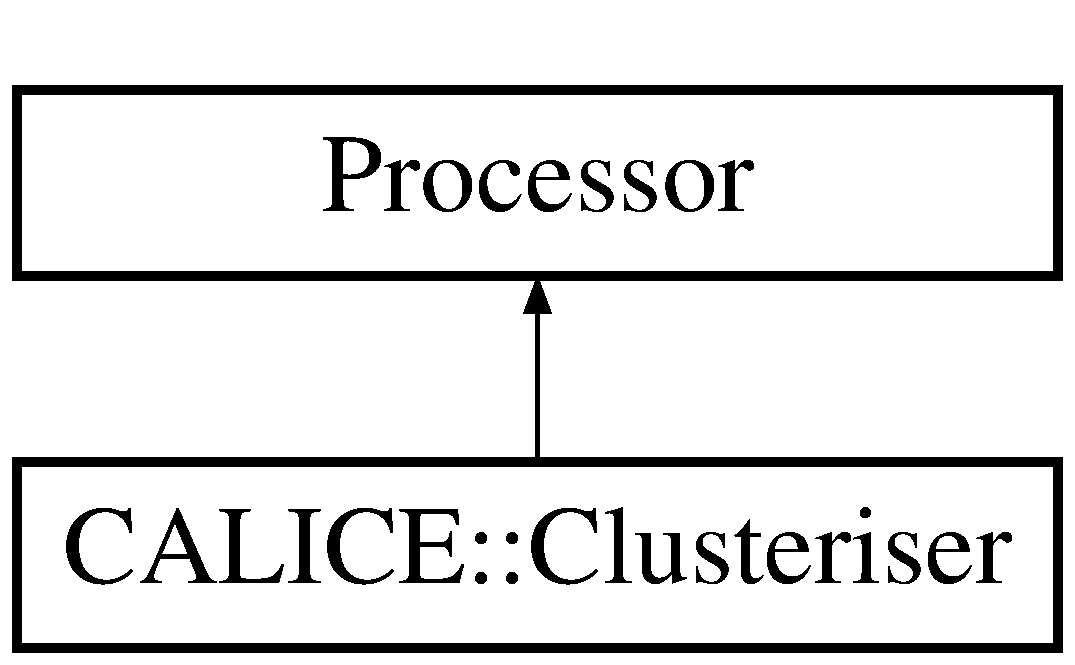
\includegraphics[height=2.000000cm]{classCALICE_1_1Clusteriser}
\end{center}
\end{figure}
\subsection*{Public Member Functions}
\begin{DoxyCompactItemize}
\item 
Processor $\ast$ {\bfseries new\-Processor} ()\label{classCALICE_1_1Clusteriser_afc7acd77a2c4c6108896d86185534533}

\item 
{\bf Clusteriser} ()
\begin{DoxyCompactList}\small\item\em Select Mips . \end{DoxyCompactList}\item 
void {\bf init} ()
\begin{DoxyCompactList}\small\item\em Called at the begin of the job before anything is read. \end{DoxyCompactList}\item 
void {\bf process\-Run\-Header} (L\-C\-Run\-Header $\ast$run)
\begin{DoxyCompactList}\small\item\em Called for every run, e.\-g. \end{DoxyCompactList}\item 
void {\bf process\-Event} (L\-C\-Event $\ast$evt\-P)\label{classCALICE_1_1Clusteriser_a1970423a42279c703863638f1b8cc298}

\begin{DoxyCompactList}\small\item\em Called for every event -\/ the working horse. \end{DoxyCompactList}\item 
void {\bfseries end} ()\label{classCALICE_1_1Clusteriser_a70d9b2bb4d1be51c3608c0e57b398926}

\end{DoxyCompactItemize}
\subsection*{Protected Attributes}
\begin{DoxyCompactItemize}
\item 
Int\-\_\-t {\bf \-\_\-n\-Hits\-Min}
\begin{DoxyCompactList}\small\item\em minimum required number of hits for a cluster (marlin processor parameter). \end{DoxyCompactList}\item 
Float\-\_\-t {\bf \-\_\-max\-Dist}
\begin{DoxyCompactList}\small\item\em the maximum distance between hits considered to be close (marlin processor parameter). \end{DoxyCompactList}\item 
Float\-\_\-t {\bf \-\_\-min\-Energy}
\begin{DoxyCompactList}\small\item\em the minimum energy required for a cluster to be accepted. \end{DoxyCompactList}\item 
Float\-\_\-t {\bf \-\_\-w0}
\begin{DoxyCompactList}\small\item\em Cut parameter which defines the energy threshold of hits considered in the centre-\/of-\/gravity determination. \end{DoxyCompactList}\item 
E\-V\-E\-N\-T\-::\-Float\-Vec {\bf \-\_\-pos\-Error}
\begin{DoxyCompactList}\small\item\em the error on the cluster position in x, y and z. \end{DoxyCompactList}\item 
std\-::string {\bf \-\_\-col\-Name}\label{classCALICE_1_1Clusteriser_af6a7832cc276de50a9c96649b5b27bc3}

\begin{DoxyCompactList}\small\item\em name of the hit input collection (Marlin processor parameter) \end{DoxyCompactList}\item 
std\-::string {\bf \-\_\-cluster\-Col\-Name}\label{classCALICE_1_1Clusteriser_a2eda1746e521ba46d07556aabdfbfb6b}

\begin{DoxyCompactList}\small\item\em name of the cluster output collection (Marlin processor parameter) \end{DoxyCompactList}\end{DoxyCompactItemize}
\subsection*{Private Attributes}
\begin{DoxyCompactItemize}
\item 
std\-::vector$<$ U\-Int\-\_\-t $>$ {\bf \-\_\-isolated\-Hits}\label{classCALICE_1_1Clusteriser_ad87b17caeede7031aa2b2e0c4dac5f53}

\begin{DoxyCompactList}\small\item\em temporary buffer \end{DoxyCompactList}\end{DoxyCompactItemize}


\subsection{Detailed Description}
Simple class to try to select hits resulting from one mip. 

This processor tries to find hits in the chosen hit collection which are close together. If the number adjacent hits is large enough a cluster is created. \begin{DoxyRefDesc}{Todo}
\item[{\bf Todo}]\-: add shower shape criterium, maximum number of tolerated hits \end{DoxyRefDesc}


Definition at line 27 of file Clusteriser.\-hh.



\subsection{Constructor \& Destructor Documentation}
\index{C\-A\-L\-I\-C\-E\-::\-Clusteriser@{C\-A\-L\-I\-C\-E\-::\-Clusteriser}!Clusteriser@{Clusteriser}}
\index{Clusteriser@{Clusteriser}!CALICE::Clusteriser@{C\-A\-L\-I\-C\-E\-::\-Clusteriser}}
\subsubsection[{Clusteriser}]{\setlength{\rightskip}{0pt plus 5cm}C\-A\-L\-I\-C\-E\-::\-Clusteriser\-::\-Clusteriser (
\begin{DoxyParamCaption}
{}
\end{DoxyParamCaption}
)}\label{classCALICE_1_1Clusteriser_af90511eeaaf5a849272c290935a9d5a2}


Select Mips . 

Mip tracks are search within the calorimeter hits. Developped for cosmics. 

Definition at line 43 of file Clusteriser.\-cc.



References \-\_\-cluster\-Col\-Name, \-\_\-col\-Name, \-\_\-max\-Dist, \-\_\-min\-Energy, \-\_\-n\-Hits\-Min, \-\_\-pos\-Error, and \-\_\-w0.



\subsection{Member Function Documentation}
\index{C\-A\-L\-I\-C\-E\-::\-Clusteriser@{C\-A\-L\-I\-C\-E\-::\-Clusteriser}!init@{init}}
\index{init@{init}!CALICE::Clusteriser@{C\-A\-L\-I\-C\-E\-::\-Clusteriser}}
\subsubsection[{init}]{\setlength{\rightskip}{0pt plus 5cm}void C\-A\-L\-I\-C\-E\-::\-Clusteriser\-::init (
\begin{DoxyParamCaption}
{}
\end{DoxyParamCaption}
)}\label{classCALICE_1_1Clusteriser_ac1461d10ca6ff3ffe4e90e248382d28d}


Called at the begin of the job before anything is read. 

Use to initialize the processor, e.\-g. book histograms. 

Definition at line 137 of file Clusteriser.\-cc.



References \-\_\-pos\-Error, and histmgr\-::\-Hist\-Mgr\-::create\-Histograms().

\index{C\-A\-L\-I\-C\-E\-::\-Clusteriser@{C\-A\-L\-I\-C\-E\-::\-Clusteriser}!process\-Run\-Header@{process\-Run\-Header}}
\index{process\-Run\-Header@{process\-Run\-Header}!CALICE::Clusteriser@{C\-A\-L\-I\-C\-E\-::\-Clusteriser}}
\subsubsection[{process\-Run\-Header}]{\setlength{\rightskip}{0pt plus 5cm}void C\-A\-L\-I\-C\-E\-::\-Clusteriser\-::process\-Run\-Header (
\begin{DoxyParamCaption}
\item[{L\-C\-Run\-Header $\ast$}]{run}
\end{DoxyParamCaption}
)\hspace{0.3cm}{\ttfamily [inline]}}\label{classCALICE_1_1Clusteriser_a243b8bcabecb882cbee9787a5b34f2c1}


Called for every run, e.\-g. 

overwrite to initialize run dependent histograms. 

Definition at line 45 of file Clusteriser.\-hh.



\subsection{Field Documentation}
\index{C\-A\-L\-I\-C\-E\-::\-Clusteriser@{C\-A\-L\-I\-C\-E\-::\-Clusteriser}!\-\_\-max\-Dist@{\-\_\-max\-Dist}}
\index{\-\_\-max\-Dist@{\-\_\-max\-Dist}!CALICE::Clusteriser@{C\-A\-L\-I\-C\-E\-::\-Clusteriser}}
\subsubsection[{\-\_\-max\-Dist}]{\setlength{\rightskip}{0pt plus 5cm}Float\-\_\-t C\-A\-L\-I\-C\-E\-::\-Clusteriser\-::\-\_\-max\-Dist\hspace{0.3cm}{\ttfamily [protected]}}\label{classCALICE_1_1Clusteriser_a807005cec4f96c8a6b5aaac0def5e81b}


the maximum distance between hits considered to be close (marlin processor parameter). 



Definition at line 55 of file Clusteriser.\-hh.



Referenced by Clusteriser(), and process\-Event().

\index{C\-A\-L\-I\-C\-E\-::\-Clusteriser@{C\-A\-L\-I\-C\-E\-::\-Clusteriser}!\-\_\-min\-Energy@{\-\_\-min\-Energy}}
\index{\-\_\-min\-Energy@{\-\_\-min\-Energy}!CALICE::Clusteriser@{C\-A\-L\-I\-C\-E\-::\-Clusteriser}}
\subsubsection[{\-\_\-min\-Energy}]{\setlength{\rightskip}{0pt plus 5cm}Float\-\_\-t C\-A\-L\-I\-C\-E\-::\-Clusteriser\-::\-\_\-min\-Energy\hspace{0.3cm}{\ttfamily [protected]}}\label{classCALICE_1_1Clusteriser_adddac3244a642b766585fdb7653b2f16}


the minimum energy required for a cluster to be accepted. 



Definition at line 56 of file Clusteriser.\-hh.



Referenced by Clusteriser(), and process\-Event().

\index{C\-A\-L\-I\-C\-E\-::\-Clusteriser@{C\-A\-L\-I\-C\-E\-::\-Clusteriser}!\-\_\-n\-Hits\-Min@{\-\_\-n\-Hits\-Min}}
\index{\-\_\-n\-Hits\-Min@{\-\_\-n\-Hits\-Min}!CALICE::Clusteriser@{C\-A\-L\-I\-C\-E\-::\-Clusteriser}}
\subsubsection[{\-\_\-n\-Hits\-Min}]{\setlength{\rightskip}{0pt plus 5cm}Int\-\_\-t C\-A\-L\-I\-C\-E\-::\-Clusteriser\-::\-\_\-n\-Hits\-Min\hspace{0.3cm}{\ttfamily [protected]}}\label{classCALICE_1_1Clusteriser_a5451dad61f977c6de41a25739c6fb97c}


minimum required number of hits for a cluster (marlin processor parameter). 



Definition at line 54 of file Clusteriser.\-hh.



Referenced by Clusteriser(), and process\-Event().

\index{C\-A\-L\-I\-C\-E\-::\-Clusteriser@{C\-A\-L\-I\-C\-E\-::\-Clusteriser}!\-\_\-pos\-Error@{\-\_\-pos\-Error}}
\index{\-\_\-pos\-Error@{\-\_\-pos\-Error}!CALICE::Clusteriser@{C\-A\-L\-I\-C\-E\-::\-Clusteriser}}
\subsubsection[{\-\_\-pos\-Error}]{\setlength{\rightskip}{0pt plus 5cm}E\-V\-E\-N\-T\-::\-Float\-Vec C\-A\-L\-I\-C\-E\-::\-Clusteriser\-::\-\_\-pos\-Error\hspace{0.3cm}{\ttfamily [protected]}}\label{classCALICE_1_1Clusteriser_a02ac68c99c5bc9a3bb259cde379316d5}


the error on the cluster position in x, y and z. 



Definition at line 60 of file Clusteriser.\-hh.



Referenced by Clusteriser(), init(), and process\-Event().

\index{C\-A\-L\-I\-C\-E\-::\-Clusteriser@{C\-A\-L\-I\-C\-E\-::\-Clusteriser}!\-\_\-w0@{\-\_\-w0}}
\index{\-\_\-w0@{\-\_\-w0}!CALICE::Clusteriser@{C\-A\-L\-I\-C\-E\-::\-Clusteriser}}
\subsubsection[{\-\_\-w0}]{\setlength{\rightskip}{0pt plus 5cm}Float\-\_\-t C\-A\-L\-I\-C\-E\-::\-Clusteriser\-::\-\_\-w0\hspace{0.3cm}{\ttfamily [protected]}}\label{classCALICE_1_1Clusteriser_aa761e8e58c6b8b4239ebccf1cf7e0f44}


Cut parameter which defines the energy threshold of hits considered in the centre-\/of-\/gravity determination. 



Definition at line 57 of file Clusteriser.\-hh.



Referenced by Clusteriser(), and process\-Event().



The documentation for this class was generated from the following files\-:\begin{DoxyCompactItemize}
\item 
Clusteriser.\-hh\item 
Clusteriser.\-cc\end{DoxyCompactItemize}

\section{C\-A\-L\-I\-C\-E\-:\-:Collection\-Histogramer Class Reference}
\label{classCALICE_1_1CollectionHistogramer}\index{C\-A\-L\-I\-C\-E\-::\-Collection\-Histogramer@{C\-A\-L\-I\-C\-E\-::\-Collection\-Histogramer}}


Collect the names of all collections which appear in the L\-C\-I\-O stream.  




{\ttfamily \#include $<$Collection\-Histogramer.\-hh$>$}

Inheritance diagram for C\-A\-L\-I\-C\-E\-:\-:Collection\-Histogramer\-:\begin{figure}[H]
\begin{center}
\leavevmode
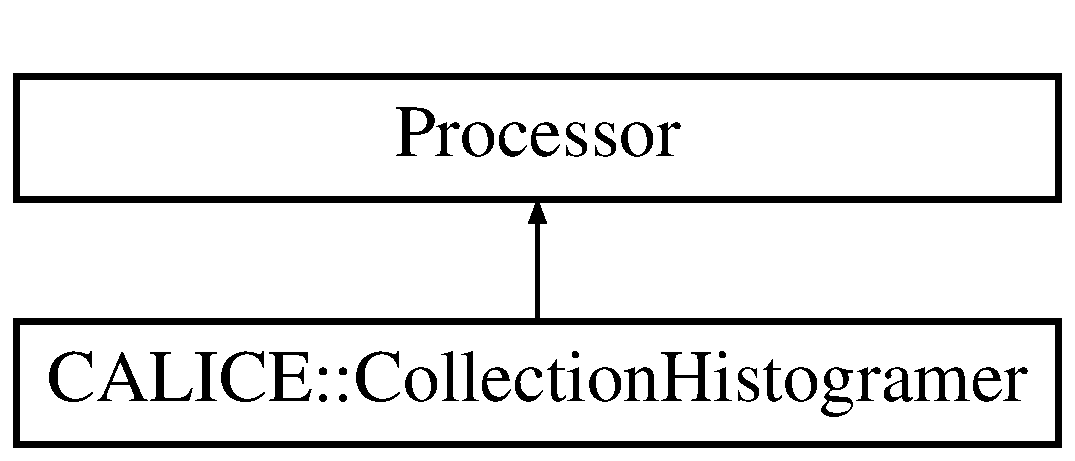
\includegraphics[height=2.000000cm]{classCALICE_1_1CollectionHistogramer}
\end{center}
\end{figure}
\subsection*{Public Member Functions}
\begin{DoxyCompactItemize}
\item 
Processor $\ast$ {\bfseries new\-Processor} ()\label{classCALICE_1_1CollectionHistogramer_ab0f528c9dbae6df5c5daad1c4a79fdce}

\item 
void {\bf init} ()
\begin{DoxyCompactList}\small\item\em Called at the begin of the job before anything is read. \end{DoxyCompactList}\item 
void {\bf process\-Run\-Header} (L\-C\-Run\-Header $\ast$run)
\begin{DoxyCompactList}\small\item\em Called for every run, e.\-g. \end{DoxyCompactList}\item 
void {\bf process\-Event} (L\-C\-Event $\ast$evt\-P)\label{classCALICE_1_1CollectionHistogramer_a35914ac7c3eb21bcb71c09ca1ae011f5}

\begin{DoxyCompactList}\small\item\em Called for every event -\/ the working horse. \end{DoxyCompactList}\item 
void {\bfseries end} ()\label{classCALICE_1_1CollectionHistogramer_a59fc5c8e1e396b6bd4268549181b2035}

\end{DoxyCompactItemize}
\subsection*{Protected Types}
\begin{DoxyCompactItemize}
\item 
enum {\bf E\-Par\-Maps} \{ \\*
{\bf k\-Collection\-Map}, 
{\bf k\-Transient\-Collection\-Map}, 
{\bf k\-Int\-Par\-Map}, 
{\bf k\-Float\-Par\-Map}, 
\\*
{\bf k\-String\-Par\-Map}, 
{\bfseries k\-N\-Par\-Maps}
 \}
\end{DoxyCompactItemize}
\subsection*{Protected Attributes}
\begin{DoxyCompactItemize}
\item 
int {\bf \-\_\-histogram\-Parameters}
\begin{DoxyCompactList}\small\item\em Set to !=0 to also histogram event parameters. \end{DoxyCompactList}\item 
std\-::map$<$ std\-::string, Average\-\_\-t $>$ {\bf \-\_\-hist} [k\-N\-Par\-Maps]
\begin{DoxyCompactList}\small\item\em collection, parameter histograms. \end{DoxyCompactList}\end{DoxyCompactItemize}
\subsection*{Static Protected Attributes}
\begin{DoxyCompactItemize}
\item 
static const char $\ast$ {\bf \-\_\-\-\_\-histogram\-Type\-Name} [k\-N\-Par\-Maps]
\begin{DoxyCompactList}\small\item\em Names for the histrogams. \end{DoxyCompactList}\end{DoxyCompactItemize}


\subsection{Detailed Description}
Collect the names of all collections which appear in the L\-C\-I\-O stream. 

Moreover some statistics are gathered about the number of elements of all the collections. 

Definition at line 16 of file Collection\-Histogramer.\-hh.



\subsection{Member Enumeration Documentation}
\index{C\-A\-L\-I\-C\-E\-::\-Collection\-Histogramer@{C\-A\-L\-I\-C\-E\-::\-Collection\-Histogramer}!E\-Par\-Maps@{E\-Par\-Maps}}
\index{E\-Par\-Maps@{E\-Par\-Maps}!CALICE::CollectionHistogramer@{C\-A\-L\-I\-C\-E\-::\-Collection\-Histogramer}}
\subsubsection[{E\-Par\-Maps}]{\setlength{\rightskip}{0pt plus 5cm}enum {\bf C\-A\-L\-I\-C\-E\-::\-Collection\-Histogramer\-::\-E\-Par\-Maps}\hspace{0.3cm}{\ttfamily [protected]}}\label{classCALICE_1_1CollectionHistogramer_aa8e603a270748b41657cbdfc32a26f19}
\begin{Desc}
\item[Enumerator]\par
\begin{description}
\index{k\-Collection\-Map@{k\-Collection\-Map}!C\-A\-L\-I\-C\-E\-::\-Collection\-Histogramer@{C\-A\-L\-I\-C\-E\-::\-Collection\-Histogramer}}\index{C\-A\-L\-I\-C\-E\-::\-Collection\-Histogramer@{C\-A\-L\-I\-C\-E\-::\-Collection\-Histogramer}!k\-Collection\-Map@{k\-Collection\-Map}}\item[{\em 
k\-Collection\-Map\label{classCALICE_1_1CollectionHistogramer_aa8e603a270748b41657cbdfc32a26f19ab623283b54710c255031397d08b2873b}
}]Normal collections. \index{k\-Transient\-Collection\-Map@{k\-Transient\-Collection\-Map}!C\-A\-L\-I\-C\-E\-::\-Collection\-Histogramer@{C\-A\-L\-I\-C\-E\-::\-Collection\-Histogramer}}\index{C\-A\-L\-I\-C\-E\-::\-Collection\-Histogramer@{C\-A\-L\-I\-C\-E\-::\-Collection\-Histogramer}!k\-Transient\-Collection\-Map@{k\-Transient\-Collection\-Map}}\item[{\em 
k\-Transient\-Collection\-Map\label{classCALICE_1_1CollectionHistogramer_aa8e603a270748b41657cbdfc32a26f19a89b047498083c3856b872694aab339d9}
}]Transient collections. \index{k\-Int\-Par\-Map@{k\-Int\-Par\-Map}!C\-A\-L\-I\-C\-E\-::\-Collection\-Histogramer@{C\-A\-L\-I\-C\-E\-::\-Collection\-Histogramer}}\index{C\-A\-L\-I\-C\-E\-::\-Collection\-Histogramer@{C\-A\-L\-I\-C\-E\-::\-Collection\-Histogramer}!k\-Int\-Par\-Map@{k\-Int\-Par\-Map}}\item[{\em 
k\-Int\-Par\-Map\label{classCALICE_1_1CollectionHistogramer_aa8e603a270748b41657cbdfc32a26f19a54df6edc6ca90f387fc046e5528c1c2a}
}]int parameters. \index{k\-Float\-Par\-Map@{k\-Float\-Par\-Map}!C\-A\-L\-I\-C\-E\-::\-Collection\-Histogramer@{C\-A\-L\-I\-C\-E\-::\-Collection\-Histogramer}}\index{C\-A\-L\-I\-C\-E\-::\-Collection\-Histogramer@{C\-A\-L\-I\-C\-E\-::\-Collection\-Histogramer}!k\-Float\-Par\-Map@{k\-Float\-Par\-Map}}\item[{\em 
k\-Float\-Par\-Map\label{classCALICE_1_1CollectionHistogramer_aa8e603a270748b41657cbdfc32a26f19aae5db92e092f27c75ae0fe2a9a159eba}
}]float parameters. \index{k\-String\-Par\-Map@{k\-String\-Par\-Map}!C\-A\-L\-I\-C\-E\-::\-Collection\-Histogramer@{C\-A\-L\-I\-C\-E\-::\-Collection\-Histogramer}}\index{C\-A\-L\-I\-C\-E\-::\-Collection\-Histogramer@{C\-A\-L\-I\-C\-E\-::\-Collection\-Histogramer}!k\-String\-Par\-Map@{k\-String\-Par\-Map}}\item[{\em 
k\-String\-Par\-Map\label{classCALICE_1_1CollectionHistogramer_aa8e603a270748b41657cbdfc32a26f19a0da7715bd0efd6aca685b31e3516f34c}
}]string parameters. \end{description}
\end{Desc}


Definition at line 47 of file Collection\-Histogramer.\-hh.



\subsection{Member Function Documentation}
\index{C\-A\-L\-I\-C\-E\-::\-Collection\-Histogramer@{C\-A\-L\-I\-C\-E\-::\-Collection\-Histogramer}!init@{init}}
\index{init@{init}!CALICE::CollectionHistogramer@{C\-A\-L\-I\-C\-E\-::\-Collection\-Histogramer}}
\subsubsection[{init}]{\setlength{\rightskip}{0pt plus 5cm}void C\-A\-L\-I\-C\-E\-::\-Collection\-Histogramer\-::init (
\begin{DoxyParamCaption}
{}
\end{DoxyParamCaption}
)}\label{classCALICE_1_1CollectionHistogramer_acbc3acffe6b5a999540387f8afb6cb36}


Called at the begin of the job before anything is read. 

Use to initialize the processor, e.\-g. book histograms. 

Definition at line 33 of file Collection\-Histogramer.\-cc.



References \-\_\-hist.

\index{C\-A\-L\-I\-C\-E\-::\-Collection\-Histogramer@{C\-A\-L\-I\-C\-E\-::\-Collection\-Histogramer}!process\-Run\-Header@{process\-Run\-Header}}
\index{process\-Run\-Header@{process\-Run\-Header}!CALICE::CollectionHistogramer@{C\-A\-L\-I\-C\-E\-::\-Collection\-Histogramer}}
\subsubsection[{process\-Run\-Header}]{\setlength{\rightskip}{0pt plus 5cm}void C\-A\-L\-I\-C\-E\-::\-Collection\-Histogramer\-::process\-Run\-Header (
\begin{DoxyParamCaption}
\item[{L\-C\-Run\-Header $\ast$}]{run}
\end{DoxyParamCaption}
)\hspace{0.3cm}{\ttfamily [inline]}}\label{classCALICE_1_1CollectionHistogramer_ae055ee45bf5b4fea658805219b6cfa5c}


Called for every run, e.\-g. 

overwrite to initialize run dependent histograms. 

Definition at line 35 of file Collection\-Histogramer.\-hh.



\subsection{Field Documentation}
\index{C\-A\-L\-I\-C\-E\-::\-Collection\-Histogramer@{C\-A\-L\-I\-C\-E\-::\-Collection\-Histogramer}!\-\_\-\-\_\-histogram\-Type\-Name@{\-\_\-\-\_\-histogram\-Type\-Name}}
\index{\-\_\-\-\_\-histogram\-Type\-Name@{\-\_\-\-\_\-histogram\-Type\-Name}!CALICE::CollectionHistogramer@{C\-A\-L\-I\-C\-E\-::\-Collection\-Histogramer}}
\subsubsection[{\-\_\-\-\_\-histogram\-Type\-Name}]{\setlength{\rightskip}{0pt plus 5cm}const char $\ast$ C\-A\-L\-I\-C\-E\-::\-Collection\-Histogramer\-::\-\_\-\-\_\-histogram\-Type\-Name\hspace{0.3cm}{\ttfamily [static]}, {\ttfamily [protected]}}\label{classCALICE_1_1CollectionHistogramer_a81e846127f3559c1e127748408ced91d}
{\bfseries Initial value\-:}
\begin{DoxyCode}
=\{
    \textcolor{stringliteral}{"Collections"}, 
    \textcolor{stringliteral}{"Transient Collections"},
    \textcolor{stringliteral}{"Integer Parameters"},
    \textcolor{stringliteral}{"Float Parameters"},
    \textcolor{stringliteral}{"String Parameters"}
  \}
\end{DoxyCode}


Names for the histrogams. 



Definition at line 55 of file Collection\-Histogramer.\-hh.

\index{C\-A\-L\-I\-C\-E\-::\-Collection\-Histogramer@{C\-A\-L\-I\-C\-E\-::\-Collection\-Histogramer}!\-\_\-hist@{\-\_\-hist}}
\index{\-\_\-hist@{\-\_\-hist}!CALICE::CollectionHistogramer@{C\-A\-L\-I\-C\-E\-::\-Collection\-Histogramer}}
\subsubsection[{\-\_\-hist}]{\setlength{\rightskip}{0pt plus 5cm}std\-::map$<$std\-::string,Average\-\_\-t$>$ C\-A\-L\-I\-C\-E\-::\-Collection\-Histogramer\-::\-\_\-hist[k\-N\-Par\-Maps]\hspace{0.3cm}{\ttfamily [protected]}}\label{classCALICE_1_1CollectionHistogramer_a9f492bba67d841ac03bdf3beeb646d8e}


collection, parameter histograms. 



Definition at line 54 of file Collection\-Histogramer.\-hh.



Referenced by init(), and process\-Event().

\index{C\-A\-L\-I\-C\-E\-::\-Collection\-Histogramer@{C\-A\-L\-I\-C\-E\-::\-Collection\-Histogramer}!\-\_\-histogram\-Parameters@{\-\_\-histogram\-Parameters}}
\index{\-\_\-histogram\-Parameters@{\-\_\-histogram\-Parameters}!CALICE::CollectionHistogramer@{C\-A\-L\-I\-C\-E\-::\-Collection\-Histogramer}}
\subsubsection[{\-\_\-histogram\-Parameters}]{\setlength{\rightskip}{0pt plus 5cm}int C\-A\-L\-I\-C\-E\-::\-Collection\-Histogramer\-::\-\_\-histogram\-Parameters\hspace{0.3cm}{\ttfamily [protected]}}\label{classCALICE_1_1CollectionHistogramer_ac12fee356ac0d035722040ca71751aa1}


Set to !=0 to also histogram event parameters. 



Definition at line 45 of file Collection\-Histogramer.\-hh.



Referenced by process\-Event().



The documentation for this class was generated from the following files\-:\begin{DoxyCompactItemize}
\item 
Collection\-Histogramer.\-hh\item 
Collection\-Histogramer.\-cc\end{DoxyCompactItemize}

\section{C\-A\-L\-I\-C\-E\-:\-:Collection\-Selector Class Reference}
\label{classCALICE_1_1CollectionSelector}\index{C\-A\-L\-I\-C\-E\-::\-Collection\-Selector@{C\-A\-L\-I\-C\-E\-::\-Collection\-Selector}}


Mark matching collections as transient or remove transient mark.  




{\ttfamily \#include $<$Collection\-Selector.\-hh$>$}

Inheritance diagram for C\-A\-L\-I\-C\-E\-:\-:Collection\-Selector\-:\begin{figure}[H]
\begin{center}
\leavevmode
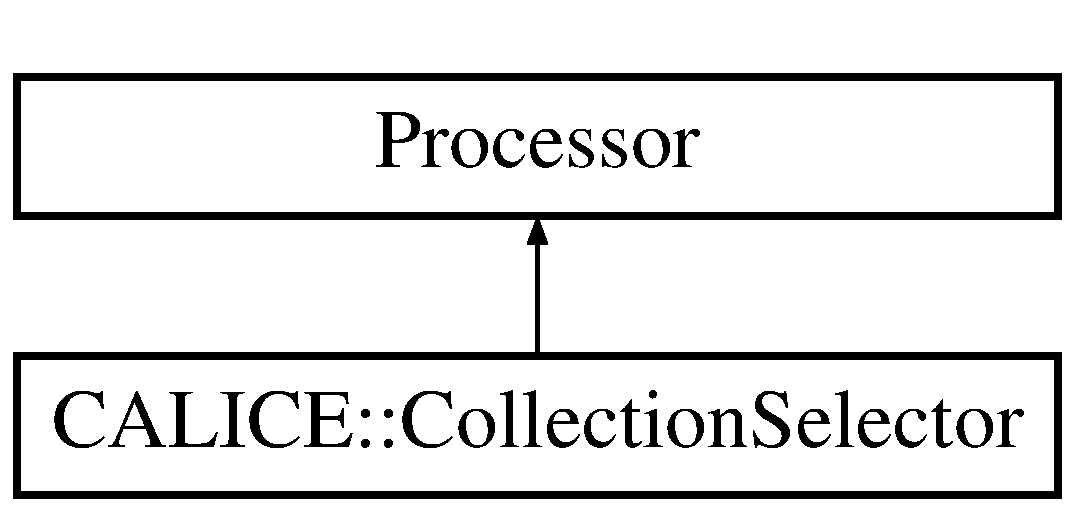
\includegraphics[height=2.000000cm]{classCALICE_1_1CollectionSelector}
\end{center}
\end{figure}
\subsection*{Public Member Functions}
\begin{DoxyCompactItemize}
\item 
Processor $\ast$ {\bfseries new\-Processor} ()\label{classCALICE_1_1CollectionSelector_abc7ca774dc191ae2c2e437d6932513ca}

\item 
void {\bf init} ()
\begin{DoxyCompactList}\small\item\em Called at the begin of the job before anything is read. \end{DoxyCompactList}\item 
void {\bf process\-Run\-Header} (L\-C\-Run\-Header $\ast$run)
\begin{DoxyCompactList}\small\item\em Called for every run, e.\-g. \end{DoxyCompactList}\item 
void {\bf process\-Event} (L\-C\-Event $\ast$evt\-P)\label{classCALICE_1_1CollectionSelector_a7fae16a6069ad23c39f9ea1498229f96}

\begin{DoxyCompactList}\small\item\em Called for every event -\/ the working horse. \end{DoxyCompactList}\item 
void {\bfseries end} ()\label{classCALICE_1_1CollectionSelector_a22ff69b0e61dada140f07cba6b1da38d}

\end{DoxyCompactItemize}
\subsection*{Static Protected Member Functions}
\begin{DoxyCompactItemize}
\item 
static void {\bf set\-Transient} (lcio\-::\-L\-C\-Event $\ast$evt\-P, const std\-::string \&name, bool transient)
\begin{DoxyCompactList}\small\item\em Set or remove the transient Mark of a collection. \end{DoxyCompactList}\end{DoxyCompactItemize}
\subsection*{Protected Attributes}
\begin{DoxyCompactItemize}
\item 
String\-Vec {\bfseries \-\_\-exclude\-Pattern}\label{classCALICE_1_1CollectionSelector_a86b479c6f8e185649ad9abd60f7368f6}

\item 
String\-Vec {\bfseries \-\_\-include\-Pattern}\label{classCALICE_1_1CollectionSelector_affaaa3265a0d7999c529145d548b4acb}

\item 
String\-Vec {\bfseries \-\_\-selection\-List}\label{classCALICE_1_1CollectionSelector_a256b9ed4988d50f352080713f747eb48}

\item 
String\-Vec {\bfseries \-\_\-selection\-Variable\-Name}\label{classCALICE_1_1CollectionSelector_a312bf14ff28957ec68c3155065a7aae4}

\item 
Int\-Vec {\bfseries \-\_\-selection\-Value}\label{classCALICE_1_1CollectionSelector_a924046461ef2a59eebafcc04184f6069}

\end{DoxyCompactItemize}


\subsection{Detailed Description}
Mark matching collections as transient or remove transient mark. 

The processor has two Parameters exclude\-Pattern, include\-Pattern. The transient flags are changed of all collections matching the exclude\-Pattern or include\-Pattern. The pattern is just a simple string. If it is contained in a collection name the collection is marked transient(exclude\-Pattern) or the transient status is removed(include\-Pattern) \begin{DoxyRefDesc}{Todo}
\item[{\bf Todo}]the simple string should be replaced by regular expressions. \end{DoxyRefDesc}


Definition at line 18 of file Collection\-Selector.\-hh.



\subsection{Member Function Documentation}
\index{C\-A\-L\-I\-C\-E\-::\-Collection\-Selector@{C\-A\-L\-I\-C\-E\-::\-Collection\-Selector}!init@{init}}
\index{init@{init}!CALICE::CollectionSelector@{C\-A\-L\-I\-C\-E\-::\-Collection\-Selector}}
\subsubsection[{init}]{\setlength{\rightskip}{0pt plus 5cm}void C\-A\-L\-I\-C\-E\-::\-Collection\-Selector\-::init (
\begin{DoxyParamCaption}
{}
\end{DoxyParamCaption}
)}\label{classCALICE_1_1CollectionSelector_acea2e18ce2a94f1b3a94bbaa1e4cc734}


Called at the begin of the job before anything is read. 

Use to initialize the processor, e.\-g. book histograms. 

Definition at line 54 of file Collection\-Selector.\-cc.

\index{C\-A\-L\-I\-C\-E\-::\-Collection\-Selector@{C\-A\-L\-I\-C\-E\-::\-Collection\-Selector}!process\-Run\-Header@{process\-Run\-Header}}
\index{process\-Run\-Header@{process\-Run\-Header}!CALICE::CollectionSelector@{C\-A\-L\-I\-C\-E\-::\-Collection\-Selector}}
\subsubsection[{process\-Run\-Header}]{\setlength{\rightskip}{0pt plus 5cm}void C\-A\-L\-I\-C\-E\-::\-Collection\-Selector\-::process\-Run\-Header (
\begin{DoxyParamCaption}
\item[{L\-C\-Run\-Header $\ast$}]{run}
\end{DoxyParamCaption}
)\hspace{0.3cm}{\ttfamily [inline]}}\label{classCALICE_1_1CollectionSelector_a81a6bfe4a27cbd181767f6e2614e80f5}


Called for every run, e.\-g. 

overwrite to initialize run dependent histograms. 

Definition at line 36 of file Collection\-Selector.\-hh.

\index{C\-A\-L\-I\-C\-E\-::\-Collection\-Selector@{C\-A\-L\-I\-C\-E\-::\-Collection\-Selector}!set\-Transient@{set\-Transient}}
\index{set\-Transient@{set\-Transient}!CALICE::CollectionSelector@{C\-A\-L\-I\-C\-E\-::\-Collection\-Selector}}
\subsubsection[{set\-Transient}]{\setlength{\rightskip}{0pt plus 5cm}void C\-A\-L\-I\-C\-E\-::\-Collection\-Selector\-::set\-Transient (
\begin{DoxyParamCaption}
\item[{lcio\-::\-L\-C\-Event $\ast$}]{evt\-P, }
\item[{const std\-::string \&}]{name, }
\item[{bool}]{transient}
\end{DoxyParamCaption}
)\hspace{0.3cm}{\ttfamily [static]}, {\ttfamily [protected]}}\label{classCALICE_1_1CollectionSelector_a712a0fa500f4d84da8804000d31f2a6e}


Set or remove the transient Mark of a collection. 


\begin{DoxyParams}{Parameters}
{\em evt\-P} & pointer to the event in which the collection transient status is altered. \\
\hline
{\em name} & name of the collection to be altered \\
\hline
{\em transient} & if equals true the collection is marked transient otherwise the transient mark is removed \\
\hline
\end{DoxyParams}


Definition at line 151 of file Collection\-Selector.\-cc.



Referenced by process\-Event().



The documentation for this class was generated from the following files\-:\begin{DoxyCompactItemize}
\item 
Collection\-Selector.\-hh\item 
Collection\-Selector.\-cc\end{DoxyCompactItemize}

\section{Constant\-Calibration Class Reference}
\label{classConstantCalibration}\index{Constant\-Calibration@{Constant\-Calibration}}


Apply the same calibration constant to all values.  




{\ttfamily \#include $<$Constant\-Calibration.\-hh$>$}

Inheritance diagram for Constant\-Calibration\-:\begin{figure}[H]
\begin{center}
\leavevmode
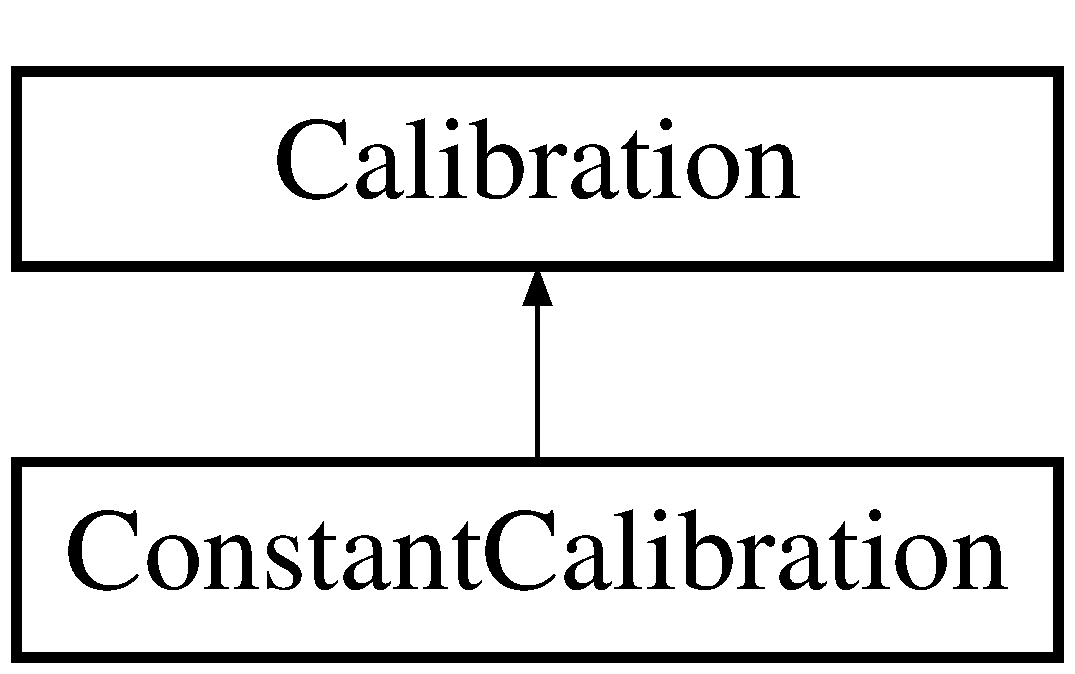
\includegraphics[height=2.000000cm]{classConstantCalibration}
\end{center}
\end{figure}
\subsection*{Public Member Functions}
\begin{DoxyCompactItemize}
\item 
{\bfseries Constant\-Calibration} (Float\-\_\-t a\-\_\-scale)\label{classConstantCalibration_ae9946996c03d02f0fdbeba232c1038f6}

\item 
Float\-\_\-t {\bf get\-Calibrated\-Value} (U\-Int\-\_\-t module\-\_\-index, U\-Int\-\_\-t module\-\_\-type, U\-Int\-\_\-t cell\-\_\-index, Float\-\_\-t adc\-\_\-value) const 
\begin{DoxyCompactList}\small\item\em Determine from a pedestal subtracted A\-D\-C value a calibrated value which are identical for this very lazy calibrator. \end{DoxyCompactList}\item 
Bool\-\_\-t {\bf check\-For\-Calibration\-Constants\-Of\-Module} (U\-Int\-\_\-t module\-\_\-id, U\-Int\-\_\-t module\-\_\-type, U\-Int\-\_\-t n\-\_\-cells) const 
\begin{DoxyCompactList}\small\item\em Verify that calibration constants exist for a certain module. \end{DoxyCompactList}\item 
Int\-\_\-t {\bf get\-Minium\-A\-D\-C\-For\-Mip\-Threshold} (Float\-\_\-t mip\-\_\-energy\-\_\-fraction) const 
\begin{DoxyCompactList}\small\item\em Get the minimum adc value mips will have for the given energy fraction on all pads. \end{DoxyCompactList}\end{DoxyCompactItemize}
\subsection*{Private Attributes}
\begin{DoxyCompactItemize}
\item 
Float\-\_\-t {\bfseries \-\_\-scale}\label{classConstantCalibration_a75406a566ee793bd4661588fe071c981}

\end{DoxyCompactItemize}


\subsection{Detailed Description}
Apply the same calibration constant to all values. 

Useful to perform a very rough calibration such that all the energy parameters, energy dependent bin limits, etc. need not be changed. The collection name of the calibration constant collection is abused to pass the scale paramer (as a string) to this class when created by the kit. 

Definition at line 14 of file Constant\-Calibration.\-hh.



\subsection{Member Function Documentation}
\index{Constant\-Calibration@{Constant\-Calibration}!check\-For\-Calibration\-Constants\-Of\-Module@{check\-For\-Calibration\-Constants\-Of\-Module}}
\index{check\-For\-Calibration\-Constants\-Of\-Module@{check\-For\-Calibration\-Constants\-Of\-Module}!ConstantCalibration@{Constant\-Calibration}}
\subsubsection[{check\-For\-Calibration\-Constants\-Of\-Module}]{\setlength{\rightskip}{0pt plus 5cm}Bool\-\_\-t Constant\-Calibration\-::check\-For\-Calibration\-Constants\-Of\-Module (
\begin{DoxyParamCaption}
\item[{U\-Int\-\_\-t}]{module\-\_\-id, }
\item[{U\-Int\-\_\-t}]{module\-\_\-type, }
\item[{U\-Int\-\_\-t}]{n\-\_\-cells}
\end{DoxyParamCaption}
) const\hspace{0.3cm}{\ttfamily [inline]}, {\ttfamily [virtual]}}\label{classConstantCalibration_aec30f5342ec651fa61708d2675e14d05}


Verify that calibration constants exist for a certain module. 


\begin{DoxyParams}{Parameters}
{\em module\-\_\-id} & id Or serial number of a module which uniquely identifies a detector module of a certain type. \\
\hline
{\em module\-\_\-type} & the type of the detector module \\
\hline
{\em n\-\_\-cells} & the number of cells on this module. Return true if calibration constants exist for the given module and the number of cells matches the number of calibration constants. \\
\hline
\end{DoxyParams}


Implements {\bf Calibration} \doxyref{}{p.}{classCalibration_a04c8f21c6e77cd3c91c858ca2c9373c4}.



Definition at line 33 of file Constant\-Calibration.\-hh.

\index{Constant\-Calibration@{Constant\-Calibration}!get\-Calibrated\-Value@{get\-Calibrated\-Value}}
\index{get\-Calibrated\-Value@{get\-Calibrated\-Value}!ConstantCalibration@{Constant\-Calibration}}
\subsubsection[{get\-Calibrated\-Value}]{\setlength{\rightskip}{0pt plus 5cm}Float\-\_\-t Constant\-Calibration\-::get\-Calibrated\-Value (
\begin{DoxyParamCaption}
\item[{U\-Int\-\_\-t}]{module\-\_\-index, }
\item[{U\-Int\-\_\-t}]{module\-\_\-type, }
\item[{U\-Int\-\_\-t}]{cell\-\_\-index, }
\item[{Float\-\_\-t}]{adc\-\_\-value}
\end{DoxyParamCaption}
) const\hspace{0.3cm}{\ttfamily [inline]}, {\ttfamily [virtual]}}\label{classConstantCalibration_a347808435c2c9e499af4c9a83d1c6915}


Determine from a pedestal subtracted A\-D\-C value a calibrated value which are identical for this very lazy calibrator. 


\begin{DoxyParams}{Parameters}
{\em module\-\_\-index} & index of the module a module is considered to be a unit which is always calibrated in one calibration run. \\
\hline
{\em module\-\_\-type} & the type of the detector module \\
\hline
{\em cell\-\_\-index} & \\
\hline
{\em adc\-\_\-value} & the A\-D\-C value which should be calibrated. \\
\hline
\end{DoxyParams}


Implements {\bf Calibration} \doxyref{}{p.}{classCalibration_aca88d93a445ba3021c05dd61b293568c}.



Definition at line 25 of file Constant\-Calibration.\-hh.

\index{Constant\-Calibration@{Constant\-Calibration}!get\-Minium\-A\-D\-C\-For\-Mip\-Threshold@{get\-Minium\-A\-D\-C\-For\-Mip\-Threshold}}
\index{get\-Minium\-A\-D\-C\-For\-Mip\-Threshold@{get\-Minium\-A\-D\-C\-For\-Mip\-Threshold}!ConstantCalibration@{Constant\-Calibration}}
\subsubsection[{get\-Minium\-A\-D\-C\-For\-Mip\-Threshold}]{\setlength{\rightskip}{0pt plus 5cm}Int\-\_\-t Constant\-Calibration\-::get\-Minium\-A\-D\-C\-For\-Mip\-Threshold (
\begin{DoxyParamCaption}
\item[{Float\-\_\-t}]{mip\-\_\-energy\-\_\-fraction}
\end{DoxyParamCaption}
) const\hspace{0.3cm}{\ttfamily [inline]}, {\ttfamily [virtual]}}\label{classConstantCalibration_ada035fed7a513d3da391bdea2c1d23f7}


Get the minimum adc value mips will have for the given energy fraction on all pads. 


\begin{DoxyParams}{Parameters}
{\em mip\-\_\-energy\-\_\-fraction} & the energy in mips \\
\hline
\end{DoxyParams}
\begin{DoxyReturn}{Returns}
minimum adc value which is below the given energy on all pads. This method can be used to get the lowest adc value a mip of the given energy fraction will have on all pads. This value is useful to select candidates before actually performing th calibration. This function is intended to be called at the beginning of each event. 
\end{DoxyReturn}


Implements {\bf Calibration} \doxyref{}{p.}{classCalibration_a4e45f1eca0d4fdf19ad76b8f581aee12}.



Definition at line 43 of file Constant\-Calibration.\-hh.



The documentation for this class was generated from the following file\-:\begin{DoxyCompactItemize}
\item 
Constant\-Calibration.\-hh\end{DoxyCompactItemize}

\section{Constant\-Calibration\-Kit Class Reference}
\label{classConstantCalibrationKit}\index{Constant\-Calibration\-Kit@{Constant\-Calibration\-Kit}}


Create a calibration object which just returns the uncalibrated values.  


Inheritance diagram for Constant\-Calibration\-Kit\-:\begin{figure}[H]
\begin{center}
\leavevmode
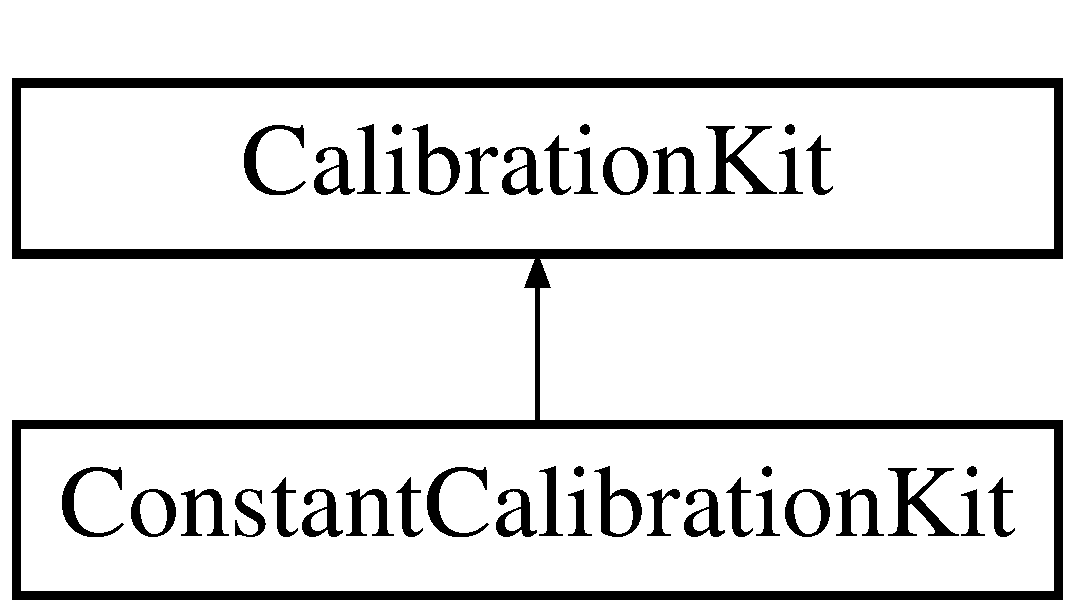
\includegraphics[height=2.000000cm]{classConstantCalibrationKit}
\end{center}
\end{figure}
\subsection*{Public Member Functions}
\begin{DoxyCompactItemize}
\item 
{\bf Calibration} $\ast$ {\bf create} (const std\-::string \&module\-\_\-type\-\_\-col\-\_\-name, const std\-::string \&module\-\_\-calibration\-\_\-col\-\_\-name) const 
\begin{DoxyCompactList}\small\item\em Create a constant calibration object. \end{DoxyCompactList}\end{DoxyCompactItemize}
\subsection*{Static Protected Attributes}
\begin{DoxyCompactItemize}
\item 
static {\bf Constant\-Calibration\-Kit} {\bfseries \-\_\-\-\_\-instance}\label{classConstantCalibrationKit_a7425667eea5619bbf2004d94030b872f}

\end{DoxyCompactItemize}


\subsection{Detailed Description}
Create a calibration object which just returns the uncalibrated values. 

The collection name of the calibration constant collection is abused to pass the scale paramer to the \doxyref{Constant\-Calibration}{p.}{classConstantCalibration} object. \begin{DoxySeeAlso}{See Also}
\doxyref{Constant\-Calibration}{p.}{classConstantCalibration}. 
\end{DoxySeeAlso}


Definition at line 13 of file Constant\-Calibration.\-cc.



\subsection{Member Function Documentation}
\index{Constant\-Calibration\-Kit@{Constant\-Calibration\-Kit}!create@{create}}
\index{create@{create}!ConstantCalibrationKit@{Constant\-Calibration\-Kit}}
\subsubsection[{create}]{\setlength{\rightskip}{0pt plus 5cm}{\bf Calibration}$\ast$ Constant\-Calibration\-Kit\-::create (
\begin{DoxyParamCaption}
\item[{const std\-::string \&}]{module\-\_\-type\-\_\-col\-\_\-name, }
\item[{const std\-::string \&}]{module\-\_\-calibration\-\_\-col\-\_\-name}
\end{DoxyParamCaption}
) const\hspace{0.3cm}{\ttfamily [inline]}, {\ttfamily [virtual]}}\label{classConstantCalibrationKit_a3b84989011be10b816104fdc58963882}


Create a constant calibration object. 


\begin{DoxyParams}{Parameters}
{\em module\-\_\-type\-\_\-col\-\_\-name} & not used. \\
\hline
{\em module\-\_\-calibration\-\_\-col\-\_\-name} & converted to a float value and passed as scale to the \doxyref{Constant\-Calibration}{p.}{classConstantCalibration} object. \\
\hline
\end{DoxyParams}


Implements {\bf Calibration\-Kit} \doxyref{}{p.}{classCalibrationKit_ab3aea5671d91a7b6f5e839324cf45a70}.



Definition at line 28 of file Constant\-Calibration.\-cc.



The documentation for this class was generated from the following file\-:\begin{DoxyCompactItemize}
\item 
Constant\-Calibration.\-cc\end{DoxyCompactItemize}

\section{marlin\-:\-:Dhc\-Raw\-Hit\-Processor Class Reference}
\label{classmarlin_1_1DhcRawHitProcessor}\index{marlin\-::\-Dhc\-Raw\-Hit\-Processor@{marlin\-::\-Dhc\-Raw\-Hit\-Processor}}


Class to process dhc raw hits and to write out Dhc\-Raw\-Calorimeter Hits.  




{\ttfamily \#include $<$Dhc\-Raw\-Hit\-Processor.\-hh$>$}

Inheritance diagram for marlin\-:\-:Dhc\-Raw\-Hit\-Processor\-:\begin{figure}[H]
\begin{center}
\leavevmode
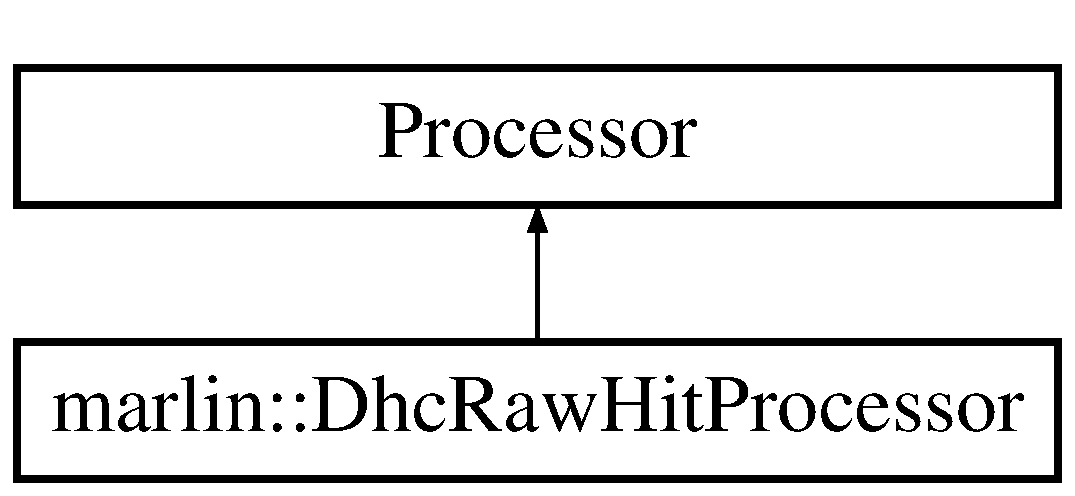
\includegraphics[height=2.000000cm]{classmarlin_1_1DhcRawHitProcessor}
\end{center}
\end{figure}
\subsection*{Public Member Functions}
\begin{DoxyCompactItemize}
\item 
virtual Processor $\ast$ {\bfseries new\-Processor} ()\label{classmarlin_1_1DhcRawHitProcessor_a60efa733ebac7b3d0a1d3f4b69a57afd}

\item 
void {\bfseries init} ()\label{classmarlin_1_1DhcRawHitProcessor_a17aeafb39578a0ce914906710afcf37c}

\item 
void {\bfseries process\-Event} (L\-C\-Event $\ast$evt)\label{classmarlin_1_1DhcRawHitProcessor_a062ebf7771719404738770b8db3967df}

\item 
void {\bfseries end} ()\label{classmarlin_1_1DhcRawHitProcessor_a61469c31a6fb75bfebc73650d91a7d54}

\end{DoxyCompactItemize}


\subsection{Detailed Description}
Class to process dhc raw hits and to write out Dhc\-Raw\-Calorimeter Hits. 

\begin{DoxyAuthor}{Author}
\-: R. P�schl D\-E\-S\-Y 
\end{DoxyAuthor}
\begin{DoxyDate}{Date}
Dec 7 2005 
\end{DoxyDate}


Definition at line 52 of file Dhc\-Raw\-Hit\-Processor.\-hh.



The documentation for this class was generated from the following files\-:\begin{DoxyCompactItemize}
\item 
Dhc\-Raw\-Hit\-Processor.\-hh\item 
Dhc\-Raw\-Hit\-Processor.\-cc\end{DoxyCompactItemize}

\section{C\-A\-L\-I\-C\-E\-:\-:Error\-Missing\-Conditions\-Data\-Handler Class Reference}
\label{classCALICE_1_1ErrorMissingConditionsDataHandler}\index{C\-A\-L\-I\-C\-E\-::\-Error\-Missing\-Conditions\-Data\-Handler@{C\-A\-L\-I\-C\-E\-::\-Error\-Missing\-Conditions\-Data\-Handler}}
Inheritance diagram for C\-A\-L\-I\-C\-E\-:\-:Error\-Missing\-Conditions\-Data\-Handler\-:\begin{figure}[H]
\begin{center}
\leavevmode
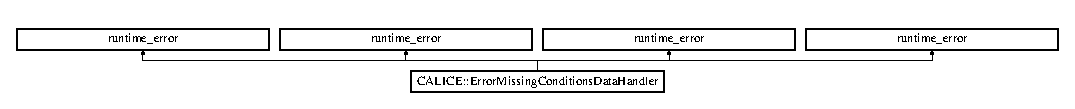
\includegraphics[height=1.021898cm]{classCALICE_1_1ErrorMissingConditionsDataHandler}
\end{center}
\end{figure}
\subsection*{Public Member Functions}
\begin{DoxyCompactItemize}
\item 
{\bfseries Error\-Missing\-Conditions\-Data\-Handler} (const std\-::string \&message)\label{classCALICE_1_1ErrorMissingConditionsDataHandler_a0a85b29547427c53f0c9f5ba5b3070b0}

\item 
{\bfseries Error\-Missing\-Conditions\-Data\-Handler} (const std\-::string \&message)\label{classCALICE_1_1ErrorMissingConditionsDataHandler_a0a85b29547427c53f0c9f5ba5b3070b0}

\item 
{\bfseries Error\-Missing\-Conditions\-Data\-Handler} (const std\-::string \&message)\label{classCALICE_1_1ErrorMissingConditionsDataHandler_a0a85b29547427c53f0c9f5ba5b3070b0}

\item 
{\bfseries Error\-Missing\-Conditions\-Data\-Handler} (const std\-::string \&message)\label{classCALICE_1_1ErrorMissingConditionsDataHandler_a0a85b29547427c53f0c9f5ba5b3070b0}

\end{DoxyCompactItemize}


\subsection{Detailed Description}


Definition at line 19 of file Base\-Mapping\-I\-I\-Processor.\-hh.



The documentation for this class was generated from the following files\-:\begin{DoxyCompactItemize}
\item 
Base\-Mapping\-I\-I\-Processor.\-hh\item 
fast\-Mapping\-I\-I\-Processor.\-hh\item 
Sc\-E\-C\-A\-L\-Mapping\-Processor.\-hh\item 
V\-Raw\-A\-D\-C\-Value\-Processor.\-hh\end{DoxyCompactItemize}

\section{T\-B\-Track\-Aligner\-:\-:Event\-Hits Class Reference}
\label{classTBTrackAligner_1_1EventHits}\index{T\-B\-Track\-Aligner\-::\-Event\-Hits@{T\-B\-Track\-Aligner\-::\-Event\-Hits}}


Method to write the histograms in a R\-O\-O\-T file.  


\subsection*{Data Fields}
\begin{DoxyCompactItemize}
\item 
std\-::vector$<$ int $>$ {\bfseries \-\_\-event\-Hits} [2][4]\label{classTBTrackAligner_1_1EventHits_afb7cf3fe9d066546baa05ea1980bf4a6}

\end{DoxyCompactItemize}


\subsection{Detailed Description}
Method to write the histograms in a R\-O\-O\-T file. 

Definition at line 54 of file T\-B\-Track\-Aligner.\-hh.



The documentation for this class was generated from the following file\-:\begin{DoxyCompactItemize}
\item 
T\-B\-Track\-Aligner.\-hh\end{DoxyCompactItemize}

\section{C\-A\-L\-I\-C\-E\-:\-:Extract\-Configuration\-Average\-Processor$<$ K\-E\-Y, V\-A\-L\-U\-E, O\-B\-J\-E\-C\-T\-\_\-\-T\-O\-\_\-\-A\-V\-E\-R\-A\-G\-E $>$ Class Template Reference}
\label{classCALICE_1_1ExtractConfigurationAverageProcessor}\index{C\-A\-L\-I\-C\-E\-::\-Extract\-Configuration\-Average\-Processor$<$ K\-E\-Y, V\-A\-L\-U\-E, O\-B\-J\-E\-C\-T\-\_\-\-T\-O\-\_\-\-A\-V\-E\-R\-A\-G\-E $>$@{C\-A\-L\-I\-C\-E\-::\-Extract\-Configuration\-Average\-Processor$<$ K\-E\-Y, V\-A\-L\-U\-E, O\-B\-J\-E\-C\-T\-\_\-\-T\-O\-\_\-\-A\-V\-E\-R\-A\-G\-E $>$}}


Processor to determine the channel-\/wise average over any type of configuration over an entire run.  




{\ttfamily \#include $<$Extract\-Configuration\-Average\-Processor.\-hh$>$}

Inheritance diagram for C\-A\-L\-I\-C\-E\-:\-:Extract\-Configuration\-Average\-Processor$<$ K\-E\-Y, V\-A\-L\-U\-E, O\-B\-J\-E\-C\-T\-\_\-\-T\-O\-\_\-\-A\-V\-E\-R\-A\-G\-E $>$\-:\begin{figure}[H]
\begin{center}
\leavevmode
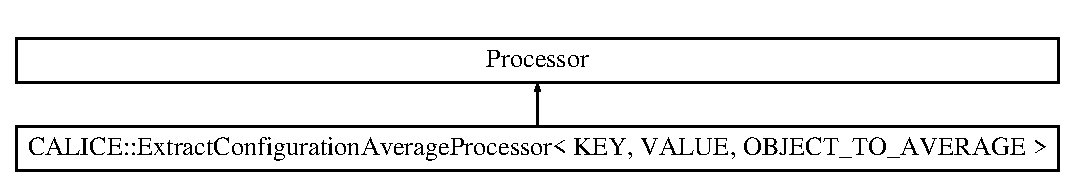
\includegraphics[height=2.000000cm]{classCALICE_1_1ExtractConfigurationAverageProcessor}
\end{center}
\end{figure}
\subsection*{Public Types}
\begin{DoxyCompactItemize}
\item 
typedef std\-::map$<$ K\-E\-Y, \\*
Average\-Value$<$ V\-A\-L\-U\-E $>$ $>$ {\bfseries Average\-Value\-Map\-\_\-t}\label{classCALICE_1_1ExtractConfigurationAverageProcessor_a9c98d937494a57cb0002414676ef0a0b}

\item 
typedef Average\-Value\-Map\-\_\-t\-::iterator {\bfseries A\-V\-M\-\_\-iterator}\label{classCALICE_1_1ExtractConfigurationAverageProcessor_af2676889c0cabe4ef45a8d0a41953f22}

\item 
typedef \\*
Average\-Value\-Map\-\_\-t\-::const\-\_\-iterator {\bfseries A\-V\-M\-\_\-const\-\_\-iterator}\label{classCALICE_1_1ExtractConfigurationAverageProcessor_ae898392ad5d30a3cf24636368c1f1817}

\item 
typedef K\-E\-Y(O\-B\-J\-E\-C\-T\-\_\-\-T\-O\-\_\-\-A\-V\-E\-R\-A\-G\-E\-::$\ast$ {\bfseries P\-M\-F\-\_\-\-K\-E\-Y} )() const \label{classCALICE_1_1ExtractConfigurationAverageProcessor_ac14ddbcd21b11b49846b2e9f6179806f}

\item 
typedef V\-A\-L\-U\-E(O\-B\-J\-E\-C\-T\-\_\-\-T\-O\-\_\-\-A\-V\-E\-R\-A\-G\-E\-::$\ast$ {\bfseries P\-M\-F\-\_\-\-V\-A\-L\-U\-E} )() const \label{classCALICE_1_1ExtractConfigurationAverageProcessor_a77c343fefe0aa8c92d90c2c841f2ba0f}

\end{DoxyCompactItemize}
\subsection*{Public Member Functions}
\begin{DoxyCompactItemize}
\item 
{\bfseries Extract\-Configuration\-Average\-Processor} (const std\-::string name, P\-M\-F\-\_\-\-K\-E\-Y pmf\-\_\-key, P\-M\-F\-\_\-\-V\-A\-L\-U\-E pmf\-\_\-value)\label{classCALICE_1_1ExtractConfigurationAverageProcessor_a8035f64050859ba76161f1432b37b457}

\item 
{\bf Extract\-Configuration\-Average\-Processor} $\ast$ {\bf new\-Processor} ()\label{classCALICE_1_1ExtractConfigurationAverageProcessor_a077ce7a15806f9843796b912eb8fbce7}

\begin{DoxyCompactList}\small\item\em Implements marlin\-::\-Processor\-::new\-Processor() \end{DoxyCompactList}\item 
virtual void {\bf init} ()\label{classCALICE_1_1ExtractConfigurationAverageProcessor_a28b4116dd4ec68e02db2c9f2ee17fc74}

\begin{DoxyCompactList}\small\item\em Implements marlin\-::\-Processor\-::init() \end{DoxyCompactList}\item 
virtual void {\bf process\-Event} (L\-C\-Event $\ast$evt)\label{classCALICE_1_1ExtractConfigurationAverageProcessor_a7e74ff5efd13293e12977cd11787dbc7}

\begin{DoxyCompactList}\small\item\em Implements marlin\-::\-Processor\-::process\-Event(\-L\-C\-Event$\ast$) \end{DoxyCompactList}\item 
virtual void {\bf process\-Run\-Header} (L\-C\-Run\-Header $\ast$run\-Header)\label{classCALICE_1_1ExtractConfigurationAverageProcessor_a3549b7175d1d32b2103f25ead4f5a5fa}

\begin{DoxyCompactList}\small\item\em Implements marlin\-::\-Processor\-::process\-Run\-Header(\-L\-C\-Run\-Header$\ast$) \end{DoxyCompactList}\item 
virtual void {\bf end} ()\label{classCALICE_1_1ExtractConfigurationAverageProcessor_a877b167e8302d7330d3b2a595ed0e824}

\begin{DoxyCompactList}\small\item\em Implements marlin\-::\-Processor\-::end() \end{DoxyCompactList}\item 
void {\bf print} (std\-::ostream \&)\label{classCALICE_1_1ExtractConfigurationAverageProcessor_a6c7e3795c5dce5f4430a3fe53a577ff4}

\begin{DoxyCompactList}\small\item\em Print channel wise mean and R\-M\-S to output stream. \end{DoxyCompactList}\item 
void {\bf write\-Simple\-File} (L\-C\-Collection $\ast$)\label{classCALICE_1_1ExtractConfigurationAverageProcessor_a6a64edef52110005a069deafdadabb30}

\begin{DoxyCompactList}\small\item\em Store results in L\-C\-I\-O file to be read in by a Simple\-File\-Handler. \end{DoxyCompactList}\item 
void {\bf write\-D\-B\-Folder} (L\-C\-Collection $\ast$)\label{classCALICE_1_1ExtractConfigurationAverageProcessor_ad81f6e7290071ff7ad46f62a268b05a9}

\begin{DoxyCompactList}\small\item\em Store results in L\-C\-C\-D database. \end{DoxyCompactList}\end{DoxyCompactItemize}
\subsection*{Protected Member Functions}
\begin{DoxyCompactItemize}
\item 
L\-C\-Collection $\ast$ {\bfseries get\-Collection} ()\label{classCALICE_1_1ExtractConfigurationAverageProcessor_a723f985ee753e55a96b5a1d484e91769}

\end{DoxyCompactItemize}
\subsection*{Protected Attributes}
\begin{DoxyCompactItemize}
\item 
std\-::string {\bfseries \-\_\-in\-Col\-Name}\label{classCALICE_1_1ExtractConfigurationAverageProcessor_a6d532e2cc4838f68332367733b4a0bd8}

\item 
std\-::string {\bfseries \-\_\-out\-Col\-Name}\label{classCALICE_1_1ExtractConfigurationAverageProcessor_a2c538c11dc9a34d75e7d2a843702f06b}

\item 
std\-::string {\bfseries \-\_\-out\-File\-Name}\label{classCALICE_1_1ExtractConfigurationAverageProcessor_ab9111f08e45c3959b0ed36aa49bc96aa}

\item 
std\-::string {\bfseries \-\_\-db\-Init}\label{classCALICE_1_1ExtractConfigurationAverageProcessor_a63aa312d9fb326bd9b868eed4d5d0e70}

\item 
std\-::string {\bfseries \-\_\-db\-Folder}\label{classCALICE_1_1ExtractConfigurationAverageProcessor_a634cc4a35f2b694cee63d1eff7e06ada}

\item 
std\-::string {\bfseries \-\_\-db\-Description}\label{classCALICE_1_1ExtractConfigurationAverageProcessor_a50d196cf146cde52ea5bb0481ce514a6}

\item 
lccd\-::\-L\-C\-C\-D\-Time\-Stamp {\bfseries \-\_\-from}\label{classCALICE_1_1ExtractConfigurationAverageProcessor_ab06f9eaf8c5bdfbecc67576231cf32cd}

\item 
lccd\-::\-L\-C\-C\-D\-Time\-Stamp {\bfseries \-\_\-till}\label{classCALICE_1_1ExtractConfigurationAverageProcessor_a6ca967970fd97f5134bb45760a1224f8}

\item 
int {\bfseries \-\_\-select\-Conf}\label{classCALICE_1_1ExtractConfigurationAverageProcessor_ac22b0611b66e8732f7b8927a8bbf70c6}

\item 
Average\-Value\-Map\-\_\-t {\bfseries \-\_\-average\-Objects}\label{classCALICE_1_1ExtractConfigurationAverageProcessor_a0fc2d84cee1e5dcb243653b8c2ac15fc}

\item 
const std\-::string {\bfseries \-\_\-default\-String}\label{classCALICE_1_1ExtractConfigurationAverageProcessor_a1f8e7e6467b59f155e0a50acfbf19859}

\end{DoxyCompactItemize}
\subsection*{Private Attributes}
\begin{DoxyCompactItemize}
\item 
P\-M\-F\-\_\-\-K\-E\-Y {\bfseries \-\_\-pmf\-\_\-key}\label{classCALICE_1_1ExtractConfigurationAverageProcessor_a8b33481b90291e374ba3386bc462f378}

\item 
P\-M\-F\-\_\-\-V\-A\-L\-U\-E {\bfseries \-\_\-pmf\-\_\-value}\label{classCALICE_1_1ExtractConfigurationAverageProcessor_a2b24536049c82fd0cbebaee159683451}

\item 
std\-::string {\bfseries \-\_\-name}\label{classCALICE_1_1ExtractConfigurationAverageProcessor_adc1336d4d2336e11746598d496e53f7e}

\end{DoxyCompactItemize}


\subsection{Detailed Description}
\subsubsection*{template$<$class K\-E\-Y, class V\-A\-L\-U\-E, class O\-B\-J\-E\-C\-T\-\_\-\-T\-O\-\_\-\-A\-V\-E\-R\-A\-G\-E$>$class C\-A\-L\-I\-C\-E\-::\-Extract\-Configuration\-Average\-Processor$<$ K\-E\-Y, V\-A\-L\-U\-E, O\-B\-J\-E\-C\-T\-\_\-\-T\-O\-\_\-\-A\-V\-E\-R\-A\-G\-E $>$}

Processor to determine the channel-\/wise average over any type of configuration over an entire run. 

This processor selects events of a pre-\/defined type of configuration (e.\-g. pedestal or L\-E\-D block) and determined the channel-\/wise average over all these events utilizing the Average\-Value class. The results get written to screen or stored to L\-C\-I\-O files/\-L\-C\-C\-D databases in form of Simple\-Value objects. Cells are identified by the Cell\-I\-D of the input hits without any further interpretation of the meaning of this number.

\begin{DoxyAuthor}{Author}
{\tt Niels.\-Meyer@desy.\-de} 
\end{DoxyAuthor}
\begin{DoxyDate}{Date}
January 2008 
\end{DoxyDate}


Definition at line 29 of file Extract\-Configuration\-Average\-Processor.\-hh.



The documentation for this class was generated from the following files\-:\begin{DoxyCompactItemize}
\item 
Extract\-Configuration\-Average\-Processor.\-hh\item 
Extract\-Configuration\-Average\-Processor.\-cc\end{DoxyCompactItemize}

\section{C\-A\-L\-I\-C\-E\-:\-:Fast\-Calib2\-D\-Processor$<$ T, str, M $>$ Class Template Reference}
\label{classCALICE_1_1FastCalib2DProcessor}\index{C\-A\-L\-I\-C\-E\-::\-Fast\-Calib2\-D\-Processor$<$ T, str, M $>$@{C\-A\-L\-I\-C\-E\-::\-Fast\-Calib2\-D\-Processor$<$ T, str, M $>$}}


Class which handles the application of a certain type T\-:L\-C\-Hcal\-Calibration\-Object to an input collection of Calice\-Hit and writes an output collection of Calice\-Hit.  




{\ttfamily \#include $<$Fast2\-D\-Calibration\-Processor.\-hh$>$}

Inheritance diagram for C\-A\-L\-I\-C\-E\-:\-:Fast\-Calib2\-D\-Processor$<$ T, str, M $>$\-:\begin{figure}[H]
\begin{center}
\leavevmode
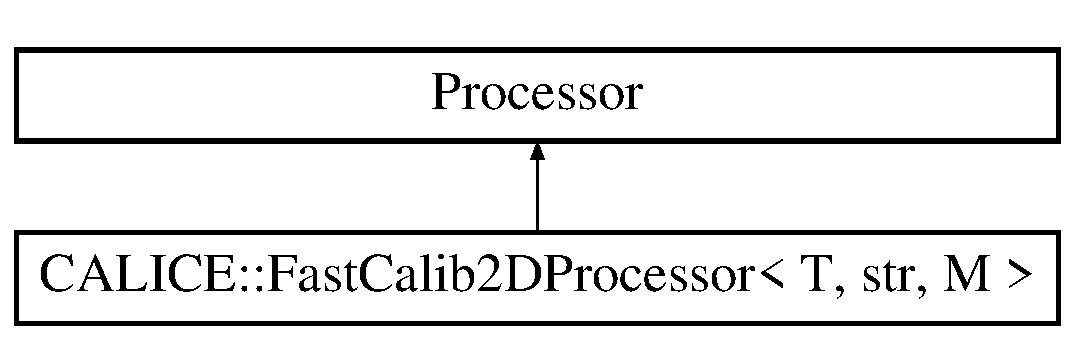
\includegraphics[height=2.000000cm]{classCALICE_1_1FastCalib2DProcessor}
\end{center}
\end{figure}
\subsection*{Public Types}
\begin{DoxyCompactItemize}
\item 
typedef std\-::map$<$ int, int $>$ {\bfseries parameter\-Map}\label{classCALICE_1_1FastCalib2DProcessor_a1a398176ac86386375acd10b92a890df}

\end{DoxyCompactItemize}
\subsection*{Public Member Functions}
\begin{DoxyCompactItemize}
\item 
virtual Processor $\ast$ {\bfseries new\-Processor} ()\label{classCALICE_1_1FastCalib2DProcessor_aba8e344351415f1bfdc0a0ab54173c27}

\item 
virtual void {\bfseries init} ()\label{classCALICE_1_1FastCalib2DProcessor_a6e39f004ac66605fac85eaf3c2303066}

\item 
void {\bfseries calibration\-Changed} (lcio\-::\-L\-C\-Collection $\ast$col)\label{classCALICE_1_1FastCalib2DProcessor_af9b944cab5d25801f3de9538ca58a5fb}

\item 
void {\bfseries ahc\-Sro\-Mod\-Data\-Col\-Changed} (lcio\-::\-L\-C\-Collection $\ast$col)\label{classCALICE_1_1FastCalib2DProcessor_ab5ffcf2162e4d6c1356e19637e407c2c}

\item 
virtual void {\bfseries process\-Event} (L\-C\-Event $\ast$evt)\label{classCALICE_1_1FastCalib2DProcessor_a9c91ffa8449e011e0f99d9e2334050ee}

\end{DoxyCompactItemize}
\subsection*{Protected Attributes}
\begin{DoxyCompactItemize}
\item 
std\-::string {\bfseries \-\_\-input\-Col\-Name}\label{classCALICE_1_1FastCalib2DProcessor_ad2a51e143d704ff9d9d33d155381fa2b}

\item 
std\-::string {\bfseries \-\_\-parameter\-Col\-Name}\label{classCALICE_1_1FastCalib2DProcessor_aeeddf47e62b3ffa578893b3e040a46c9}

\item 
std\-::string {\bfseries \-\_\-output\-Col\-Name}\label{classCALICE_1_1FastCalib2DProcessor_a67e450d381f338c512bfb61950adc5d8}

\item 
std\-::string {\bfseries \-\_\-cal\-Col\-Name}\label{classCALICE_1_1FastCalib2DProcessor_acea129179d4f2e8c00901817a63448ab}

\item 
std\-::string {\bfseries \-\_\-ahc\-Sro\-Mod\-Data\-Col\-Name}\label{classCALICE_1_1FastCalib2DProcessor_aa1d4ac2e926484e24dd1dbdaf72ea2d5}

\item 
Int\-Vec {\bfseries \-\_\-modules}\label{classCALICE_1_1FastCalib2DProcessor_a510d4c71eeac41329b513092d81f37e4}

\item 
bool {\bfseries \-\_\-overwrite}\label{classCALICE_1_1FastCalib2DProcessor_ad4f708e7935bc324ce4df8a2ab97cae2}

\item 
int {\bfseries \-\_\-zero\-Suppression}\label{classCALICE_1_1FastCalib2DProcessor_a3ced223e8bc88a1530a2edd1a2336b5e}

\item 
{\bf Calibration\-Set}$<$ T $>$ $\ast$ {\bfseries \-\_\-calib\-Set}\label{classCALICE_1_1FastCalib2DProcessor_a8bc3270235a8c869a5b8d72d74709bce}

\item 
M $\ast$ {\bfseries \-\_\-temp\-Model}\label{classCALICE_1_1FastCalib2DProcessor_a12febd0f31953e9426311be25b2a4aaa}

\end{DoxyCompactItemize}
\subsection*{Private Attributes}
\begin{DoxyCompactItemize}
\item 
Conditions\-Change\-Delegator\\*
$<$ {\bf Fast\-Calib2\-D\-Processor}$<$ T, str, \\*
M $>$ $>$ {\bfseries \-\_\-calibration\-Change}\label{classCALICE_1_1FastCalib2DProcessor_a54d843931315ba73e99210c44c5fca78}

\item 
Conditions\-Change\-Delegator\\*
$<$ {\bf Fast\-Calib2\-D\-Processor}$<$ T, str, \\*
M $>$ $>$ {\bfseries \-\_\-ahc\-Sro\-Mod\-Data\-Change}\label{classCALICE_1_1FastCalib2DProcessor_a407c59825c0f396ed42aa93e2fa1f3b9}

\item 
lcio\-::\-L\-C\-Collection $\ast$ {\bfseries \-\_\-ahc\-Sro\-Mod\-Data\-Col}\label{classCALICE_1_1FastCalib2DProcessor_ae08612f9f4ea6ec8638027e52549fbe7}

\end{DoxyCompactItemize}


\subsection{Detailed Description}
\subsubsection*{template$<$class T, const char $\ast$ str, class M = Temp\-Model$>$class C\-A\-L\-I\-C\-E\-::\-Fast\-Calib2\-D\-Processor$<$ T, str, M $>$}

Class which handles the application of a certain type T\-:L\-C\-Hcal\-Calibration\-Object to an input collection of Calice\-Hit and writes an output collection of Calice\-Hit. 

Definition at line 37 of file Fast2\-D\-Calibration\-Processor.\-hh.



The documentation for this class was generated from the following file\-:\begin{DoxyCompactItemize}
\item 
Fast2\-D\-Calibration\-Processor.\-hh\end{DoxyCompactItemize}

\section{C\-A\-L\-I\-C\-E\-:\-:Fast\-Calib\-Processor$<$ T, H, str, M $>$ Class Template Reference}
\label{classCALICE_1_1FastCalibProcessor}\index{C\-A\-L\-I\-C\-E\-::\-Fast\-Calib\-Processor$<$ T, H, str, M $>$@{C\-A\-L\-I\-C\-E\-::\-Fast\-Calib\-Processor$<$ T, H, str, M $>$}}


Class which handles the application of a certain type T\-:L\-C\-Hcal\-Calibration\-Object to an input collection of Calice\-Hit and writes an output collection of Calice\-Hit.  




{\ttfamily \#include $<$Fast\-Calibration\-Processor.\-hh$>$}

Inheritance diagram for C\-A\-L\-I\-C\-E\-:\-:Fast\-Calib\-Processor$<$ T, H, str, M $>$\-:\begin{figure}[H]
\begin{center}
\leavevmode
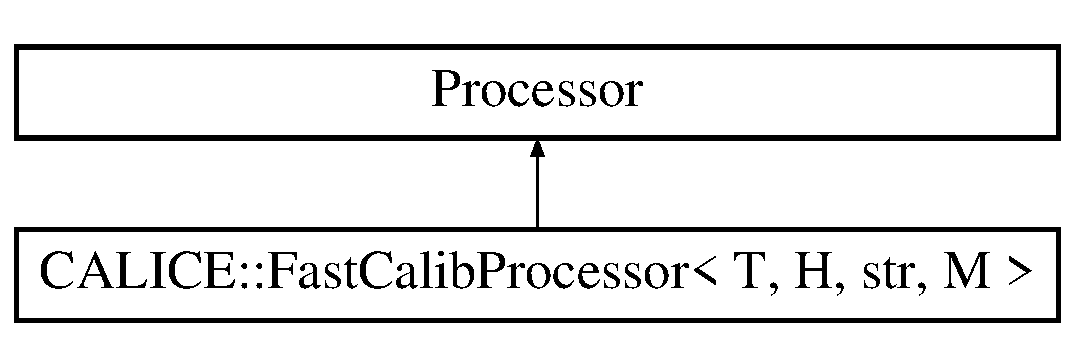
\includegraphics[height=2.000000cm]{classCALICE_1_1FastCalibProcessor}
\end{center}
\end{figure}
\subsection*{Public Member Functions}
\begin{DoxyCompactItemize}
\item 
virtual Processor $\ast$ {\bfseries new\-Processor} ()\label{classCALICE_1_1FastCalibProcessor_a3118254e508e231dd79614ed367b1de0}

\item 
virtual void {\bfseries init} ()\label{classCALICE_1_1FastCalibProcessor_a4b47376d1de4a95324feb266d3e04fe2}

\item 
void {\bfseries calibration\-Changed} (lcio\-::\-L\-C\-Collection $\ast$col)\label{classCALICE_1_1FastCalibProcessor_af0849f090e34dfa2a136d07188141064}

\item 
void {\bfseries ahc\-Sro\-Mod\-Data\-Col\-Changed} (lcio\-::\-L\-C\-Collection $\ast$col)\label{classCALICE_1_1FastCalibProcessor_a16d81154984d0fef91516ecc4d727a7f}

\item 
virtual void {\bfseries process\-Event} (L\-C\-Event $\ast$evt)\label{classCALICE_1_1FastCalibProcessor_a9f3a0e4a323ef030adc45d40d023ecff}

\end{DoxyCompactItemize}
\subsection*{Protected Attributes}
\begin{DoxyCompactItemize}
\item 
std\-::string {\bfseries \-\_\-input\-Col\-Name}\label{classCALICE_1_1FastCalibProcessor_a4e3450182079803160b3a3d49fe52bf5}

\item 
std\-::string {\bfseries \-\_\-output\-Col\-Name}\label{classCALICE_1_1FastCalibProcessor_a6ca793dcf8a511d5fcf2092c99592227}

\item 
std\-::string {\bfseries \-\_\-cal\-Col\-Name}\label{classCALICE_1_1FastCalibProcessor_a5bad8e294f9a71589ff02e911a789add}

\item 
std\-::string {\bfseries \-\_\-ahc\-Sro\-Mod\-Data\-Col\-Name}\label{classCALICE_1_1FastCalibProcessor_afe4587e7dccde530034ae8560295ab2a}

\item 
Int\-Vec {\bfseries \-\_\-modules}\label{classCALICE_1_1FastCalibProcessor_a279d5d4b719e274a887135f1bca70330}

\item 
bool {\bfseries \-\_\-overwrite}\label{classCALICE_1_1FastCalibProcessor_af756fa4e02404c38b78806a8333ecebd}

\item 
int {\bfseries \-\_\-zero\-Suppression}\label{classCALICE_1_1FastCalibProcessor_a579d58dc12aa93fb27a6dc7ae2b6654c}

\item 
bool {\bfseries \-\_\-do\-Mip\-Calibration}\label{classCALICE_1_1FastCalibProcessor_a396e71ec9015968a395f1d0d1727c897}

\item 
{\bf Calibration\-Set}$<$ T $>$ $\ast$ {\bfseries \-\_\-calib\-Set}\label{classCALICE_1_1FastCalibProcessor_add7475797b98bee61c39b503d5195dc5}

\item 
M $\ast$ {\bfseries \-\_\-temp\-Model}\label{classCALICE_1_1FastCalibProcessor_a6e48c942ee98efaf387e15e82c90fed7}

\end{DoxyCompactItemize}
\subsection*{Private Attributes}
\begin{DoxyCompactItemize}
\item 
Conditions\-Change\-Delegator\\*
$<$ {\bf Fast\-Calib\-Processor}$<$ T, H, \\*
str, M $>$ $>$ {\bfseries \-\_\-calibration\-Change}\label{classCALICE_1_1FastCalibProcessor_ae17b4d2b8c9107594ae92e70dcf2983d}

\item 
Conditions\-Change\-Delegator\\*
$<$ {\bf Fast\-Calib\-Processor}$<$ T, H, \\*
str, M $>$ $>$ {\bfseries \-\_\-ahc\-Sro\-Mod\-Data\-Change}\label{classCALICE_1_1FastCalibProcessor_a132d6fff627c0b45c1e98fc9d5a28146}

\item 
lcio\-::\-L\-C\-Collection $\ast$ {\bfseries \-\_\-ahc\-Sro\-Mod\-Data\-Col}\label{classCALICE_1_1FastCalibProcessor_ad11ad45f2892496a8582b31aea2f0fcb}

\end{DoxyCompactItemize}


\subsection{Detailed Description}
\subsubsection*{template$<$class T, class H, const char $\ast$ str, class M = Temp\-Model$>$class C\-A\-L\-I\-C\-E\-::\-Fast\-Calib\-Processor$<$ T, H, str, M $>$}

Class which handles the application of a certain type T\-:L\-C\-Hcal\-Calibration\-Object to an input collection of Calice\-Hit and writes an output collection of Calice\-Hit. 

\begin{DoxyAuthor}{Author}
S.\-Schmidt, D\-E\-S\-Y 
\end{DoxyAuthor}
\begin{DoxyDate}{Date}
Sep 23 2006 
\end{DoxyDate}


Definition at line 34 of file Fast\-Calibration\-Processor.\-hh.



The documentation for this class was generated from the following file\-:\begin{DoxyCompactItemize}
\item 
Fast\-Calibration\-Processor.\-hh\end{DoxyCompactItemize}

\section{C\-A\-L\-I\-C\-E\-:\-:fast\-Mapping\-I\-I\-Processor Class Reference}
\label{classCALICE_1_1fastMappingIIProcessor}\index{C\-A\-L\-I\-C\-E\-::fast\-Mapping\-I\-I\-Processor@{C\-A\-L\-I\-C\-E\-::fast\-Mapping\-I\-I\-Processor}}


A class which converts Calice\-Hits with all calibrations applied into Calorimeter\-Hits.  




{\ttfamily \#include $<$fast\-Mapping\-I\-I\-Processor.\-hh$>$}

Inheritance diagram for C\-A\-L\-I\-C\-E\-:\-:fast\-Mapping\-I\-I\-Processor\-:\begin{figure}[H]
\begin{center}
\leavevmode
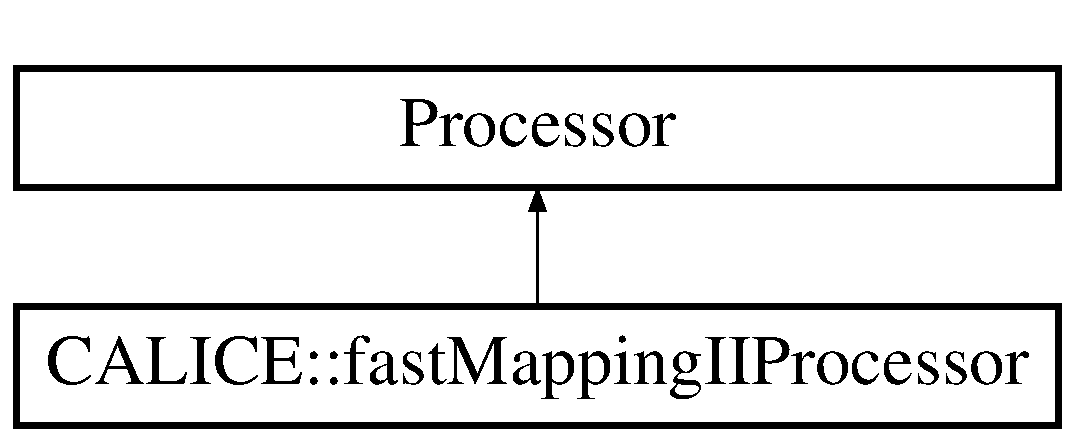
\includegraphics[height=2.000000cm]{classCALICE_1_1fastMappingIIProcessor}
\end{center}
\end{figure}
\subsection*{Public Member Functions}
\begin{DoxyCompactItemize}
\item 
virtual Processor $\ast$ {\bfseries new\-Processor} ()\label{classCALICE_1_1fastMappingIIProcessor_a84d864c37b51a69f3a5bb3336d11290b}

\item 
virtual void {\bfseries init} ()\label{classCALICE_1_1fastMappingIIProcessor_ad804302fd35900a04771a1647ee9584c}

\item 
virtual void {\bfseries process\-Run\-Header} (L\-C\-Run\-Header $\ast$run)\label{classCALICE_1_1fastMappingIIProcessor_a4dcdb93e7877928387c0da90288cd243}

\item 
virtual void {\bfseries process\-Event} (L\-C\-Event $\ast$evt)\label{classCALICE_1_1fastMappingIIProcessor_ae133d2ea34fae73e13cbbb23d567eef6}

\item 
virtual void {\bfseries check} (L\-C\-Event $\ast$evt)\label{classCALICE_1_1fastMappingIIProcessor_ade7ed6e2dea19fb8b0dce38bececbab4}

\item 
virtual void {\bfseries end} ()\label{classCALICE_1_1fastMappingIIProcessor_a720b8590ee681bb8f78bca09370129b7}

\end{DoxyCompactItemize}
\subsection*{Protected Member Functions}
\begin{DoxyCompactItemize}
\item 
virtual void {\bfseries update\-Inverse\-Map} ()\label{classCALICE_1_1fastMappingIIProcessor_ac8554c8b7fe9ed1e0ca25a08eeb8f527}

\item 
virtual void {\bfseries module\-Type\-Changed} (lcio\-::\-L\-C\-Collection $\ast$col)\label{classCALICE_1_1fastMappingIIProcessor_a28c17f0864be618ad5168c9849f1ea01}

\item 
virtual void {\bfseries module\-Location\-Changed} (lcio\-::\-L\-C\-Collection $\ast$col)\label{classCALICE_1_1fastMappingIIProcessor_aaa57f57f89b2b16635dba790b60c212c}

\item 
virtual void {\bfseries module\-Connection\-Changed} (lcio\-::\-L\-C\-Collection $\ast$col)\label{classCALICE_1_1fastMappingIIProcessor_a06bf0a87fa87dd8ed6bd979b8fbeb86b}

\item 
virtual void {\bfseries detector\-Transformation\-Changed} (lcio\-::\-L\-C\-Collection $\ast$col)\label{classCALICE_1_1fastMappingIIProcessor_a40c88849c1b343429941a7b64553aa63}

\item 
virtual void {\bfseries reference\-Transformation\-Changed} (lcio\-::\-L\-C\-Collection $\ast$col)\label{classCALICE_1_1fastMappingIIProcessor_a13db4be9a8c31bb01a20915394007d12}

\item 
virtual void {\bfseries stage\-Position\-Changed} (lcio\-::\-L\-C\-Collection $\ast$col)\label{classCALICE_1_1fastMappingIIProcessor_af962a3c913e7154e79d52ca661526e38}

\end{DoxyCompactItemize}
\subsection*{Protected Attributes}
\begin{DoxyCompactItemize}
\item 
std\-::string {\bfseries \-\_\-input\-Col\-Name}\label{classCALICE_1_1fastMappingIIProcessor_a406af5c65eb5b7fae75a9106701a41ce}

\item 
std\-::string {\bfseries \-\_\-output\-Col\-Name}\label{classCALICE_1_1fastMappingIIProcessor_a0ed73861a50691a4514c0444354d1731}

\item 
std\-::string {\bfseries \-\_\-col\-Name\-Module\-Description}\label{classCALICE_1_1fastMappingIIProcessor_a915ba9b5892f04844a61ccc01614db62}

\item 
std\-::string {\bfseries \-\_\-col\-Name\-Module\-Location}\label{classCALICE_1_1fastMappingIIProcessor_ac65181dd90dbb0696ab38e0a8ff6c164}

\item 
std\-::string {\bfseries \-\_\-col\-Name\-Module\-Connection}\label{classCALICE_1_1fastMappingIIProcessor_acfa571d0e14c1121db44ebc355a561f1}

\item 
std\-::string {\bfseries \-\_\-col\-Name\-Detector\-Transformation}\label{classCALICE_1_1fastMappingIIProcessor_af7bcda3e2cda9ee7e41dcf780243c1fd}

\item 
std\-::string {\bfseries \-\_\-col\-Name\-Reference\-Transformation}\label{classCALICE_1_1fastMappingIIProcessor_a7d554688321a42669be0482eac40daf3}

\item 
std\-::string {\bfseries \-\_\-col\-Name\-Stage\-Collection}\label{classCALICE_1_1fastMappingIIProcessor_ac85b4eccc768ff4ca78280aaadab1402}

\item 
Conditions\-Change\-Delegator\\*
$<$ {\bf fast\-Mapping\-I\-I\-Processor} $>$ {\bfseries \-\_\-module\-Type\-Change}\label{classCALICE_1_1fastMappingIIProcessor_a3bec21933dd1ca7dec20c925ec4a502a}

\item 
Conditions\-Change\-Delegator\\*
$<$ {\bf fast\-Mapping\-I\-I\-Processor} $>$ {\bfseries \-\_\-module\-Location\-Change}\label{classCALICE_1_1fastMappingIIProcessor_ac210ebf21a676091fbc1c481c90705b0}

\item 
Conditions\-Change\-Delegator\\*
$<$ {\bf fast\-Mapping\-I\-I\-Processor} $>$ {\bfseries \-\_\-module\-Connection\-Change}\label{classCALICE_1_1fastMappingIIProcessor_a1313dddb8ca17fb34b960428e1458635}

\item 
Conditions\-Change\-Delegator\\*
$<$ {\bf fast\-Mapping\-I\-I\-Processor} $>$ {\bfseries \-\_\-detector\-Transformation\-Change}\label{classCALICE_1_1fastMappingIIProcessor_ad0ad5353b297ad496673e4cddb12b4b6}

\item 
Conditions\-Change\-Delegator\\*
$<$ {\bf fast\-Mapping\-I\-I\-Processor} $>$ {\bfseries \-\_\-reference\-Transformation\-Change}\label{classCALICE_1_1fastMappingIIProcessor_a237eeddbe142d84c163d3449224ec161}

\item 
Conditions\-Change\-Delegator\\*
$<$ {\bf fast\-Mapping\-I\-I\-Processor} $>$ {\bfseries \-\_\-stage\-Position\-Change}\label{classCALICE_1_1fastMappingIIProcessor_a5f259d239bffa8e68990f72199009810}

\item 
Mapping\-And\-Alignment {\bfseries \-\_\-mapping}\label{classCALICE_1_1fastMappingIIProcessor_ad9dbad825d7b12c0e384651966588f32}

\item 
int {\bfseries \-\_\-view\-Connection\-Tree}\label{classCALICE_1_1fastMappingIIProcessor_a5512a3532b85add946d846b64112ff3c}

\item 
std\-::map$<$ unsigned, unsigned $>$ {\bfseries \-\_\-inverse\-Module\-Map}\label{classCALICE_1_1fastMappingIIProcessor_a608616991c0a6a9aacc5230b676d059c}

\end{DoxyCompactItemize}


\subsection{Detailed Description}
A class which converts Calice\-Hits with all calibrations applied into Calorimeter\-Hits. 

\begin{DoxyAuthor}{Author}
S.\-Schmidt D\-E\-S\-Y 
\end{DoxyAuthor}
\begin{DoxyDate}{Date}
July 31 2006 
\end{DoxyDate}


Definition at line 30 of file fast\-Mapping\-I\-I\-Processor.\-hh.



The documentation for this class was generated from the following files\-:\begin{DoxyCompactItemize}
\item 
fast\-Mapping\-I\-I\-Processor.\-hh\item 
fast\-Mapping\-I\-I\-Processor.\-cc\end{DoxyCompactItemize}

\section{C\-A\-L\-I\-C\-E\-:\-:fast\-Mapping\-I\-Processor Class Reference}
\label{classCALICE_1_1fastMappingIProcessor}\index{C\-A\-L\-I\-C\-E\-::fast\-Mapping\-I\-Processor@{C\-A\-L\-I\-C\-E\-::fast\-Mapping\-I\-Processor}}
Inheritance diagram for C\-A\-L\-I\-C\-E\-:\-:fast\-Mapping\-I\-Processor\-:\begin{figure}[H]
\begin{center}
\leavevmode
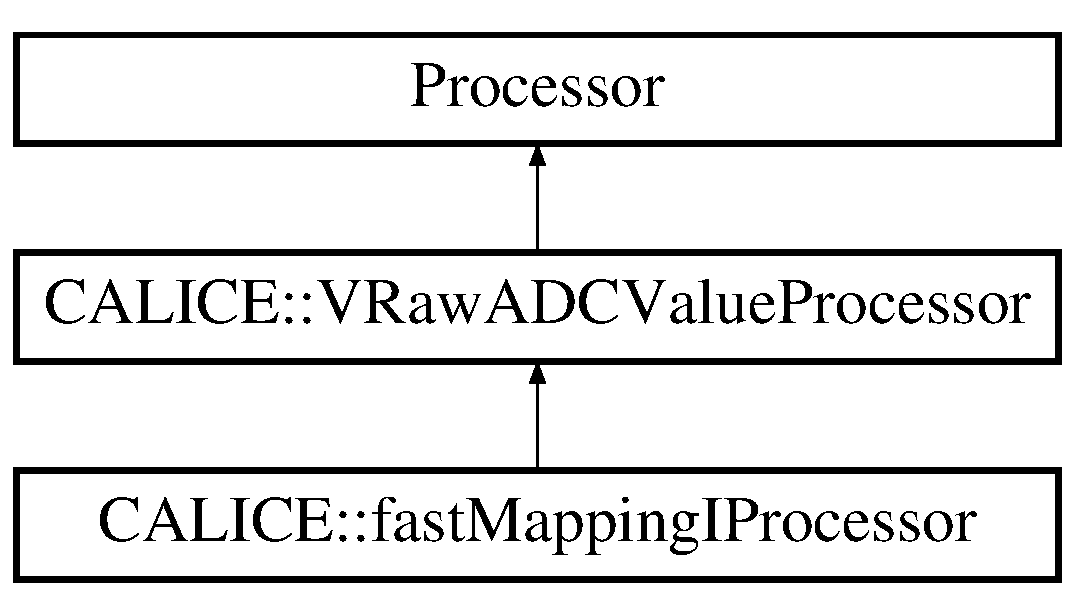
\includegraphics[height=3.000000cm]{classCALICE_1_1fastMappingIProcessor}
\end{center}
\end{figure}
\subsection*{Public Member Functions}
\begin{DoxyCompactItemize}
\item 
virtual Processor $\ast$ {\bfseries new\-Processor} ()\label{classCALICE_1_1fastMappingIProcessor_afd4a773dc4a748fd0b0f158145633c1e}

\item 
virtual void {\bfseries init} ()\label{classCALICE_1_1fastMappingIProcessor_a793005abfe7163deb7e8b358f8ba0b1c}

\item 
virtual void {\bfseries process\-Run\-Header} (L\-C\-Run\-Header $\ast$run)\label{classCALICE_1_1fastMappingIProcessor_a8b6727abbeb2da17115f390a0a98ad27}

\item 
virtual void {\bfseries process\-Event} (L\-C\-Event $\ast$evt)\label{classCALICE_1_1fastMappingIProcessor_a1a148ed309dc4126bebefd8b665e99da}

\item 
virtual void {\bfseries check} (L\-C\-Event $\ast$evt)\label{classCALICE_1_1fastMappingIProcessor_a29d4f13330cd1f1a81348412eb9f019f}

\item 
virtual void {\bfseries end} ()\label{classCALICE_1_1fastMappingIProcessor_a68fd91bd4b382f7edf96c209be10afc3}

\end{DoxyCompactItemize}
\subsection*{Protected Attributes}
\begin{DoxyCompactItemize}
\item 
std\-::string {\bfseries \-\_\-output\-Col\-Name}\label{classCALICE_1_1fastMappingIProcessor_a8c3d3a56fa6562d42d5232e1d59793d5}

\item 
int {\bfseries \-\_\-view\-Connection\-Tree}\label{classCALICE_1_1fastMappingIProcessor_a0c9ffa75645122f519a515e0cc9f03c4}

\item 
int {\bfseries \-\_\-pick\-Module}\label{classCALICE_1_1fastMappingIProcessor_a60b71c57578009091da75ae814ac787b}

\end{DoxyCompactItemize}
\subsection*{Additional Inherited Members}


\subsection{Detailed Description}


Definition at line 26 of file fast\-Mapping\-I\-Processor.\-hh.



The documentation for this class was generated from the following files\-:\begin{DoxyCompactItemize}
\item 
fast\-Mapping\-I\-Processor.\-hh\item 
fast\-Mapping\-I\-Processor.\-cc\end{DoxyCompactItemize}

\section{C\-A\-L\-I\-C\-E\-:\-:Filter\-Bad\-Channels Class Reference}
\label{classCALICE_1_1FilterBadChannels}\index{C\-A\-L\-I\-C\-E\-::\-Filter\-Bad\-Channels@{C\-A\-L\-I\-C\-E\-::\-Filter\-Bad\-Channels}}
Inheritance diagram for C\-A\-L\-I\-C\-E\-:\-:Filter\-Bad\-Channels\-:\begin{figure}[H]
\begin{center}
\leavevmode
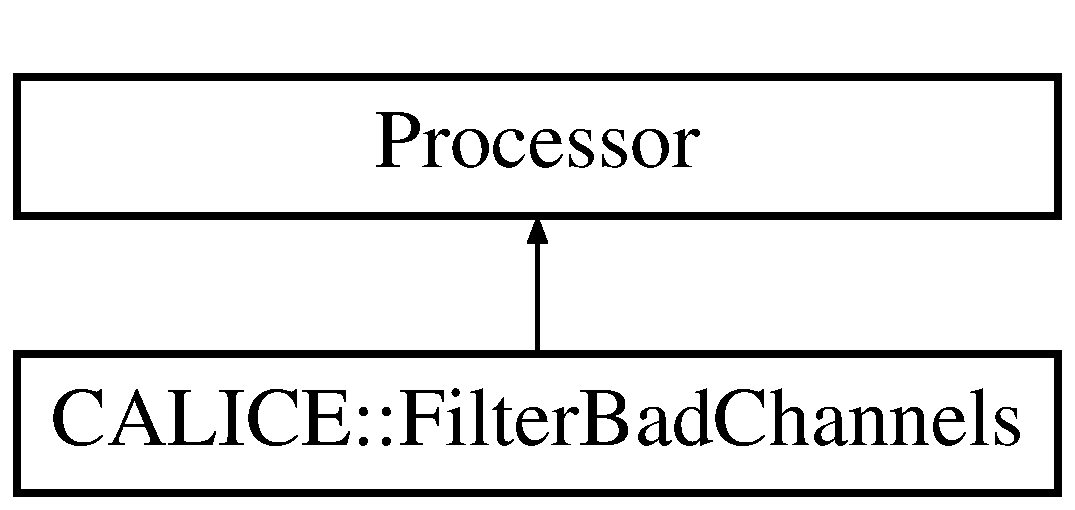
\includegraphics[height=2.000000cm]{classCALICE_1_1FilterBadChannels}
\end{center}
\end{figure}
\subsection*{Public Member Functions}
\begin{DoxyCompactItemize}
\item 
{\bf Filter\-Bad\-Channels} $\ast$ {\bfseries new\-Processor} ()\label{classCALICE_1_1FilterBadChannels_a06ad29f11701e24e64b82daa9b36b4ba}

\item 
virtual void {\bfseries init} ()\label{classCALICE_1_1FilterBadChannels_ad75699cb8a346a1dcf712a5c4a8709d9}

\item 
virtual void {\bfseries process\-Event} (L\-C\-Event $\ast$evt)\label{classCALICE_1_1FilterBadChannels_a96a8e4be917781a9f4612e44ad4f61c3}

\item 
virtual void {\bfseries end} ()\label{classCALICE_1_1FilterBadChannels_ac6a5d35d02c2b6c7dcd81a4c37126b2d}

\end{DoxyCompactItemize}
\subsection*{Private Types}
\begin{DoxyCompactItemize}
\item 
typedef lccd\-::\-Conditions\-Map\\*
$<$ const int, Cell\-Quality $>$ {\bfseries Map\-\_\-t}\label{classCALICE_1_1FilterBadChannels_ac0393be0651c887dd3b47a40e186ddfa}

\end{DoxyCompactItemize}
\subsection*{Private Attributes}
\begin{DoxyCompactItemize}
\item 
std\-::string {\bfseries \-\_\-in\-Col\-Name}\label{classCALICE_1_1FilterBadChannels_a7febc615df3c8f9df80b96a3a23e629d}

\item 
std\-::string {\bfseries \-\_\-out\-Col\-Name}\label{classCALICE_1_1FilterBadChannels_af44ac7aeffb09195d2dc225ce3ce903b}

\item 
std\-::string {\bfseries \-\_\-status\-Col\-Name}\label{classCALICE_1_1FilterBadChannels_a011f53f4dda0d7dbc98bf73579d05c95}

\item 
Map\-\_\-t $\ast$ {\bfseries \-\_\-status\-Map}\label{classCALICE_1_1FilterBadChannels_aa6be96b02055f381369ec71ab5d989fd}

\end{DoxyCompactItemize}


\subsection{Detailed Description}


Definition at line 13 of file Filter\-Bad\-Channels.\-hh.



The documentation for this class was generated from the following files\-:\begin{DoxyCompactItemize}
\item 
Filter\-Bad\-Channels.\-hh\item 
Filter\-Bad\-Channels.\-cc\end{DoxyCompactItemize}

\section{T\-B\-Track\-:\-:Fit\-Constants Class Reference}
\label{classTBTrack_1_1FitConstants}\index{T\-B\-Track\-::\-Fit\-Constants@{T\-B\-Track\-::\-Fit\-Constants}}
\subsection*{Public Types}
\begin{DoxyCompactItemize}
\item 
enum {\bfseries Particle} \{ {\bfseries electron}, 
{\bfseries hadron}
 \}
\item 
enum \{ {\bfseries number\-Of\-Ints} =0
 \}
\item 
enum \{ {\bfseries number\-Of\-Floats} =0
 \}
\item 
enum \{ {\bfseries number\-Of\-Doubles} =3 + 2$\ast$2 + 2$\ast$3 + 2$\ast$4 + 2$\ast$2$\ast$21 + 2$\ast$2$\ast$21 + 2$\ast$4 + 4
 \}
\end{DoxyCompactItemize}
\subsection*{Public Member Functions}
\begin{DoxyCompactItemize}
\item 
{\bfseries Fit\-Constants} (unsigned e=1, double err=0.\-0)\label{classTBTrack_1_1FitConstants_a47ddb6700da0d5c104eb0c369d80911e}

\item 
double {\bfseries p\-Beam} () const \label{classTBTrack_1_1FitConstants_a133ea6b18d89af235a741119259e0dbb}

\item 
void {\bfseries p\-Beam} (double p)\label{classTBTrack_1_1FitConstants_a9ce9a2d41aa782c4298a72d5c0eb209c}

\item 
void {\bfseries p\-Beam\-Scale} (double p)\label{classTBTrack_1_1FitConstants_a6af5bc62244d18b251e7954368ecb9c9}

\item 
double {\bfseries z\-Calorimeter} () const \label{classTBTrack_1_1FitConstants_acdbec3521ff0b24abf68178cc2f2618b}

\item 
void {\bfseries z\-Calorimeter} (double z)\label{classTBTrack_1_1FitConstants_af8a150ebd1d2265be0a0640aa58fac87}

\item 
double {\bfseries z\-Beam} () const \label{classTBTrack_1_1FitConstants_a4375d97e5d050aebd2b9462bbf215c75}

\item 
void {\bfseries z\-Beam} (double z)\label{classTBTrack_1_1FitConstants_afe66619121004ae499b40341e0d78eaf}

\item 
double {\bfseries beam\-Coordinate} (unsigned d) const \label{classTBTrack_1_1FitConstants_ad67c0f98da288bdaa426ee94a25056e1}

\item 
void {\bfseries beam\-Coordinate} (unsigned d, double c)\label{classTBTrack_1_1FitConstants_a999f0fc68f7ddbf17fa49fc77b2ca542}

\item 
double {\bfseries beam\-Angle} (unsigned d) const \label{classTBTrack_1_1FitConstants_ada6619cbead5a277f3a99df287094fb5}

\item 
void {\bfseries beam\-Angle} (unsigned d, double a)\label{classTBTrack_1_1FitConstants_a52e266c03c76f8bc27b2eae2f731618d}

\item 
void {\bfseries beam\-Average} (unsigned d, double c, double a)\label{classTBTrack_1_1FitConstants_a973118ce9e89a90aaa0453ad2693dc41}

\item 
T\-Matrix\-D\-Sym {\bfseries beam\-Spread} (unsigned d) const \label{classTBTrack_1_1FitConstants_a92a42dc3339b8d8812aaf9b3e96d757d}

\item 
void {\bfseries beam\-Spread} (unsigned d, const T\-Matrix\-D\-Sym \&e)\label{classTBTrack_1_1FitConstants_ad904d24cd02a69767b6935e5a3131aa2}

\item 
double {\bfseries z\-Layer} (unsigned d, unsigned l) const \label{classTBTrack_1_1FitConstants_a48d3c08ed8a147b4fe34bb0671650fda}

\item 
void {\bfseries z\-Layer} (unsigned d, unsigned l, double z)\label{classTBTrack_1_1FitConstants_afb9283b46152570709ecf4e2ceba940a}

\item 
T\-Matrix\-D\-Sym {\bfseries forward\-Scattering} (unsigned d, Particle p) const \label{classTBTrack_1_1FitConstants_a5d182698ad7f662247a7f9bf15662cd7}

\item 
void {\bfseries forward\-Scattering} (unsigned d, Particle p, const T\-Matrix\-D\-Sym \&e)\label{classTBTrack_1_1FitConstants_a1ba9942b8faf3f662fd5002a9b2f9d29}

\item 
T\-Matrix\-D\-Sym {\bfseries backward\-Scattering} (unsigned d, Particle p) const \label{classTBTrack_1_1FitConstants_aa2760e9bcaf3ca95fd18d111c2789544}

\item 
void {\bfseries backward\-Scattering} (unsigned d, Particle p, const T\-Matrix\-D\-Sym \&e)\label{classTBTrack_1_1FitConstants_ae3c4ce5580e332d5bcf1c53077f130f7}

\item 
double {\bfseries c\-Error} (unsigned d, unsigned l) const \label{classTBTrack_1_1FitConstants_aa59b427cb93906ae61d18515e656ea05}

\item 
void {\bfseries c\-Error} (unsigned d, unsigned l, double e)\label{classTBTrack_1_1FitConstants_aaa2f3eef3f50ce8ef1c3be75268024c7}

\item 
double {\bfseries probability\-Cut} (unsigned n\-Dof) const \label{classTBTrack_1_1FitConstants_a05ec4b2aba5904d2ba510d5b237e740a}

\item 
void {\bfseries probability\-Cut} (unsigned n\-Dof, double c)\label{classTBTrack_1_1FitConstants_a19530322178881f38211053231b8719c}

\item 
{\bf Track\-Fit\-Initialisation} {\bfseries fit\-Initialisation} (unsigned xy, unsigned fb, unsigned eh) const \label{classTBTrack_1_1FitConstants_a39d3a5bdfce8fe17387e1470d00543b6}

\item 
void {\bfseries write\-Icc} () const \label{classTBTrack_1_1FitConstants_ac5738f5f948c0cee82dab1ca7b5b756b}

\item 
std\-::ostream \& {\bfseries print} (std\-::ostream \&o=std\-::cout, const std\-::string \&s=\char`\"{}\char`\"{}) const \label{classTBTrack_1_1FitConstants_ad62ddbd9b8fd5f827fccabf35691abf1}

\item 
const int $\ast$ {\bfseries int\-Data} () const \label{classTBTrack_1_1FitConstants_a300c624cc611cb716f86dd7692c6f2ab}

\item 
int $\ast$ {\bfseries int\-Data} ()\label{classTBTrack_1_1FitConstants_a40b7f0a0888a062b84b4c0f47e7aa932}

\item 
const float $\ast$ {\bfseries float\-Data} () const \label{classTBTrack_1_1FitConstants_ae20c4d5c95c45bad29c9b8f364614e78}

\item 
float $\ast$ {\bfseries float\-Data} ()\label{classTBTrack_1_1FitConstants_abb376a6b05cc1c2bafb24ba44a230348}

\item 
const double $\ast$ {\bfseries double\-Data} () const \label{classTBTrack_1_1FitConstants_a05fa985c01f9de23dbffbe275afa0127}

\item 
double $\ast$ {\bfseries double\-Data} ()\label{classTBTrack_1_1FitConstants_a53ba2da4d9d0a108988e207f665c88bd}

\end{DoxyCompactItemize}
\subsection*{Private Member Functions}
\begin{DoxyCompactItemize}
\item 
void {\bfseries convert\-Error\-Matrix} (const double $\ast$d, T\-Matrix\-D\-Sym \&e) const \label{classTBTrack_1_1FitConstants_a239bf750e8846e198310ccd5dfc27b51}

\item 
void {\bfseries convert\-Error\-Matrix} (const T\-Matrix\-D\-Sym \&e, double $\ast$d)\label{classTBTrack_1_1FitConstants_aed80acea11b9312ca325f0032c2aa624}

\item 
void {\bfseries p\-Beam\-Scale} (double $\ast$mat, double p)\label{classTBTrack_1_1FitConstants_a9bb5f5ac9c07dfb702e48c48a1dce9ea}

\end{DoxyCompactItemize}
\subsection*{Private Attributes}
\begin{DoxyCompactItemize}
\item 
double {\bfseries \-\_\-p\-Beam}\label{classTBTrack_1_1FitConstants_ad065c37d27302f166d583e92ff813e08}

\item 
double {\bfseries \-\_\-z\-Calorimeter}\label{classTBTrack_1_1FitConstants_aed3664e51cc6fc58c48e8b2f9ced4b32}

\item 
double {\bfseries \-\_\-z\-Beam}\label{classTBTrack_1_1FitConstants_a038e07323028e6f0307fa69685359301}

\item 
double {\bfseries \-\_\-beam\-Average} [2][2]\label{classTBTrack_1_1FitConstants_a701a22a05bbfdc8678fbb11f0a4a6242}

\item 
double {\bfseries \-\_\-beam\-Spread} [2][3]\label{classTBTrack_1_1FitConstants_a4d9da5ca3637928a5248e53e6b42cef8}

\item 
double {\bfseries \-\_\-z\-Layer} [2][4]\label{classTBTrack_1_1FitConstants_a93f27485f5ce91ac23ffbb9febf4f8f7}

\item 
double {\bfseries \-\_\-forward\-Scattering} [2][2][21]\label{classTBTrack_1_1FitConstants_a4a9803ee41a2659da3513e4df42fd349}

\item 
double {\bfseries \-\_\-backward\-Scattering} [2][2][21]\label{classTBTrack_1_1FitConstants_ab45f453a56ff58df89b085202ee14bf3}

\item 
double {\bfseries \-\_\-c\-Error} [2][4]\label{classTBTrack_1_1FitConstants_a2fafd67579669f4e2c291fd30370be36}

\item 
double {\bfseries \-\_\-probability\-Cut} [4]\label{classTBTrack_1_1FitConstants_a7c1fb70c3f9c89d6213b34ccdf88dc67}

\end{DoxyCompactItemize}


\subsection{Detailed Description}


Definition at line 18 of file Fit\-Constants.\-hh.



The documentation for this class was generated from the following files\-:\begin{DoxyCompactItemize}
\item 
Fit\-Constants.\-hh\item 
Fit\-Constants.\-cc\end{DoxyCompactItemize}

\section{histmgr\-:\-:Float\-Histogram1\-D Class Reference}
\label{classhistmgr_1_1FloatHistogram1D}\index{histmgr\-::\-Float\-Histogram1\-D@{histmgr\-::\-Float\-Histogram1\-D}}


A 1-\/dimensional histogram using float values for the bins.  




{\ttfamily \#include $<$Float\-Histogram1\-D.\-hh$>$}

Inheritance diagram for histmgr\-:\-:Float\-Histogram1\-D\-:\begin{figure}[H]
\begin{center}
\leavevmode
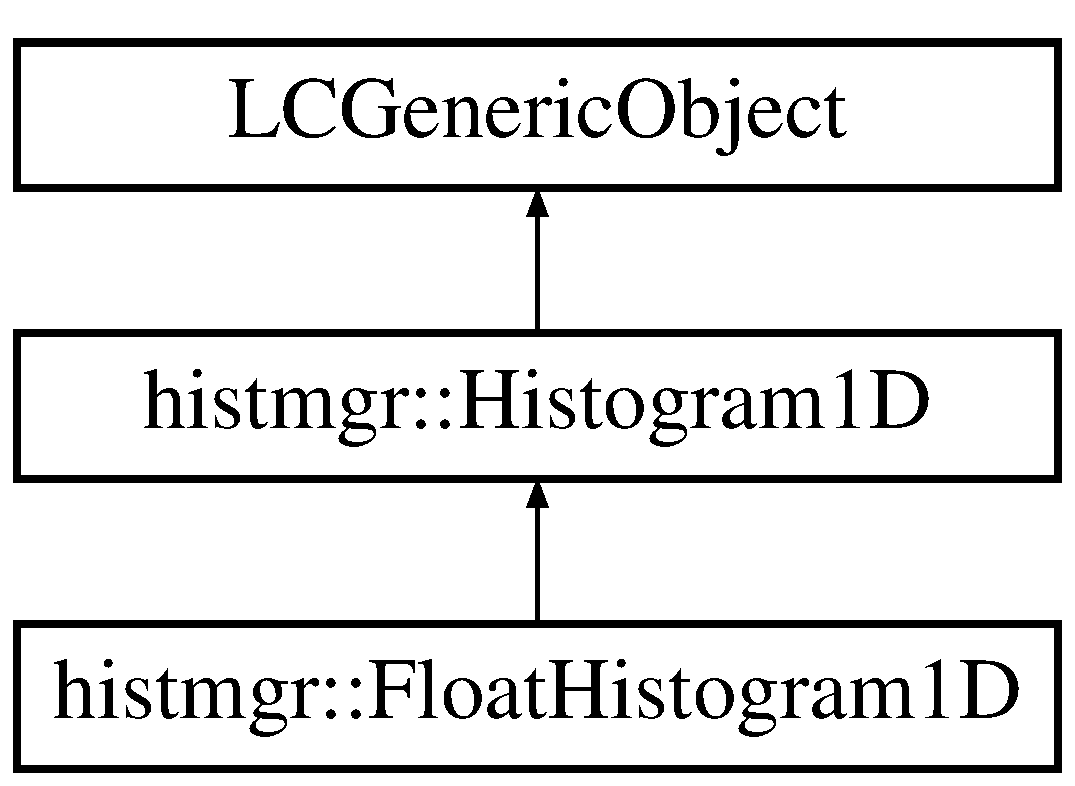
\includegraphics[height=3.000000cm]{classhistmgr_1_1FloatHistogram1D}
\end{center}
\end{figure}
\subsection*{Public Member Functions}
\begin{DoxyCompactItemize}
\item 
{\bf Float\-Histogram1\-D} (U\-Int\-\_\-t {\bf id}, const {\bf Hist\-Par} \&binning)
\begin{DoxyCompactList}\small\item\em Create a histogram with a certain binning. \end{DoxyCompactList}\item 
{\bfseries Float\-Histogram1\-D} (lcio\-::\-L\-C\-Object $\ast$a\-\_\-obj)\label{classhistmgr_1_1FloatHistogram1D_a1032bc84dcbaa4a6210fb0ee6b5088d7}

\item 
{\bfseries Float\-Histogram1\-D} (const {\bf Float\-Histogram1\-D} \&a)\label{classhistmgr_1_1FloatHistogram1D_af31379e3a83520eac73d5c1609002303}

\item 
void {\bf fill} (Float\-\_\-t value, Float\-\_\-t weight=1.)\label{classhistmgr_1_1FloatHistogram1D_aef71989b1c5ad2fc370ee96fb4022213}

\begin{DoxyCompactList}\small\item\em fill a value into the histogram \end{DoxyCompactList}\item 
void {\bf reset} ()\label{classhistmgr_1_1FloatHistogram1D_ab6020a2d0902ddc0d6b6f21ae6c579d9}

\begin{DoxyCompactList}\small\item\em reset the histograms and the number of entries \end{DoxyCompactList}\item 
void {\bf add\-To\-Bin\-Content} (U\-Int\-\_\-t bin\-\_\-index, Float\-\_\-t value)\label{classhistmgr_1_1FloatHistogram1D_ad0af3ba0d429ed031d43def85d3ca602}

\begin{DoxyCompactList}\small\item\em manipulate a histogram bin \end{DoxyCompactList}\item 
void {\bf set\-Bin\-Content} (U\-Int\-\_\-t bin\-\_\-index, Float\-\_\-t value)\label{classhistmgr_1_1FloatHistogram1D_a7c3aa74ff2e33c25678d73a0e127ef9f}

\begin{DoxyCompactList}\small\item\em manipulate a histogram bin \end{DoxyCompactList}\item 
Float\-\_\-t {\bfseries bin\-Content} (U\-Int\-\_\-t bin\-\_\-index) const \label{classhistmgr_1_1FloatHistogram1D_a4c772776ba9504a01b41bfdcbc3d4739}

\item 
Float\-\_\-t {\bfseries overflow} () const \label{classhistmgr_1_1FloatHistogram1D_ac043cc91548219a4ed8b499fa3f213cd}

\item 
Float\-\_\-t {\bfseries underflow} () const \label{classhistmgr_1_1FloatHistogram1D_a07f92873077aa35c2f8f615595909f8f}

\item 
Float\-\_\-t {\bfseries mean} () const \label{classhistmgr_1_1FloatHistogram1D_aa62d227b19581c5ad0cb0fa38706c870}

\item 
Float\-\_\-t {\bf rms} () const 
\begin{DoxyCompactList}\small\item\em Root mean square as defined by R\-O\-O\-T. \end{DoxyCompactList}\item 
Float\-\_\-t {\bf variance} () const 
\begin{DoxyCompactList}\small\item\em Variance. \end{DoxyCompactList}\item 
Double\-\_\-t {\bf integral} (U\-Int\-\_\-t first\-\_\-bin, U\-Int\-\_\-t last\-\_\-bin) const 
\begin{DoxyCompactList}\small\item\em sum contentes of bins within the given range \end{DoxyCompactList}\item 
lcio\-::\-L\-C\-Object $\ast$ {\bfseries clone} () const \label{classhistmgr_1_1FloatHistogram1D_a5edd2500f06f2b1bfd015d9ae4639175}

\end{DoxyCompactItemize}
\subsection*{Additional Inherited Members}


\subsection{Detailed Description}
A 1-\/dimensional histogram using float values for the bins. 

Definition at line 12 of file Float\-Histogram1\-D.\-hh.



\subsection{Constructor \& Destructor Documentation}
\index{histmgr\-::\-Float\-Histogram1\-D@{histmgr\-::\-Float\-Histogram1\-D}!Float\-Histogram1\-D@{Float\-Histogram1\-D}}
\index{Float\-Histogram1\-D@{Float\-Histogram1\-D}!histmgr::FloatHistogram1D@{histmgr\-::\-Float\-Histogram1\-D}}
\subsubsection[{Float\-Histogram1\-D}]{\setlength{\rightskip}{0pt plus 5cm}histmgr\-::\-Float\-Histogram1\-D\-::\-Float\-Histogram1\-D (
\begin{DoxyParamCaption}
\item[{U\-Int\-\_\-t}]{id, }
\item[{const {\bf Hist\-Par} \&}]{binning}
\end{DoxyParamCaption}
)}\label{classhistmgr_1_1FloatHistogram1D_a582ec9a1017297a5e56d159aeb18e2b9}


Create a histogram with a certain binning. 


\begin{DoxyParams}{Parameters}
{\em id} & a unique histogram I\-D, \\
\hline
{\em binning} & number of bins and range of the axis \\
\hline
\end{DoxyParams}
\begin{DoxyRefDesc}{Todo}
\item[{\bf Todo}]a name would be better than an I\-D but a string can not be easily stored in an L\-C\-Generic\-Object \end{DoxyRefDesc}


Definition at line 8 of file Float\-Histogram1\-D.\-cc.



References Hist\-Par\-::n\-Bins(), reset(), and histmgr\-::\-Histogram1\-D\-::set\-Binning().



\subsection{Member Function Documentation}
\index{histmgr\-::\-Float\-Histogram1\-D@{histmgr\-::\-Float\-Histogram1\-D}!integral@{integral}}
\index{integral@{integral}!histmgr::FloatHistogram1D@{histmgr\-::\-Float\-Histogram1\-D}}
\subsubsection[{integral}]{\setlength{\rightskip}{0pt plus 5cm}Double\-\_\-t histmgr\-::\-Float\-Histogram1\-D\-::integral (
\begin{DoxyParamCaption}
\item[{U\-Int\-\_\-t}]{first\-\_\-bin, }
\item[{U\-Int\-\_\-t}]{last\-\_\-bin}
\end{DoxyParamCaption}
) const}\label{classhistmgr_1_1FloatHistogram1D_ae4ac2bba1858e9d7750306df22c12903}


sum contentes of bins within the given range 


\begin{DoxyParams}{Parameters}
{\em first\-\_\-bin} & index of the first bin \\
\hline
{\em last\-\_\-bin} & index of the last bin (included in the sum) \\
\hline
\end{DoxyParams}
\begin{DoxyReturn}{Returns}
the sum of the bins 
\end{DoxyReturn}


Definition at line 109 of file Float\-Histogram1\-D.\-cc.

\index{histmgr\-::\-Float\-Histogram1\-D@{histmgr\-::\-Float\-Histogram1\-D}!rms@{rms}}
\index{rms@{rms}!histmgr::FloatHistogram1D@{histmgr\-::\-Float\-Histogram1\-D}}
\subsubsection[{rms}]{\setlength{\rightskip}{0pt plus 5cm}Float\-\_\-t histmgr\-::\-Float\-Histogram1\-D\-::rms (
\begin{DoxyParamCaption}
{}
\end{DoxyParamCaption}
) const}\label{classhistmgr_1_1FloatHistogram1D_a62605cd667af31082c3db712bc6ee337}


Root mean square as defined by R\-O\-O\-T. 

divided by n 

Definition at line 61 of file Float\-Histogram1\-D.\-cc.



References histmgr\-::\-Histogram1\-D\-::entries(), histmgr\-::\-Histogram1\-D\-::first\-Bin\-Index(), histmgr\-::\-Histogram1\-D\-::last\-Bin\-Index(), histmgr\-::\-Histogram1\-D\-::n\-Bins(), histmgr\-::\-Histogram1\-D\-::x\-Max(), and histmgr\-::\-Histogram1\-D\-::x\-Min().

\index{histmgr\-::\-Float\-Histogram1\-D@{histmgr\-::\-Float\-Histogram1\-D}!variance@{variance}}
\index{variance@{variance}!histmgr::FloatHistogram1D@{histmgr\-::\-Float\-Histogram1\-D}}
\subsubsection[{variance}]{\setlength{\rightskip}{0pt plus 5cm}Float\-\_\-t histmgr\-::\-Float\-Histogram1\-D\-::variance (
\begin{DoxyParamCaption}
{}
\end{DoxyParamCaption}
) const}\label{classhistmgr_1_1FloatHistogram1D_acb30c407ee9ad3bbdb85c208d6c8aee6}


Variance. 

divided by n-\/1 

Definition at line 85 of file Float\-Histogram1\-D.\-cc.



References histmgr\-::\-Histogram1\-D\-::entries(), histmgr\-::\-Histogram1\-D\-::first\-Bin\-Index(), histmgr\-::\-Histogram1\-D\-::last\-Bin\-Index(), histmgr\-::\-Histogram1\-D\-::n\-Bins(), histmgr\-::\-Histogram1\-D\-::x\-Max(), and histmgr\-::\-Histogram1\-D\-::x\-Min().



The documentation for this class was generated from the following files\-:\begin{DoxyCompactItemize}
\item 
Float\-Histogram1\-D.\-hh\item 
Float\-Histogram1\-D.\-cc\end{DoxyCompactItemize}

\section{histmgr\-:\-:Float\-Histogram2\-D Class Reference}
\label{classhistmgr_1_1FloatHistogram2D}\index{histmgr\-::\-Float\-Histogram2\-D@{histmgr\-::\-Float\-Histogram2\-D}}


A 1-\/dimensional histogram using float values for the bins.  




{\ttfamily \#include $<$Float\-Histogram2\-D.\-hh$>$}

Inheritance diagram for histmgr\-:\-:Float\-Histogram2\-D\-:\begin{figure}[H]
\begin{center}
\leavevmode
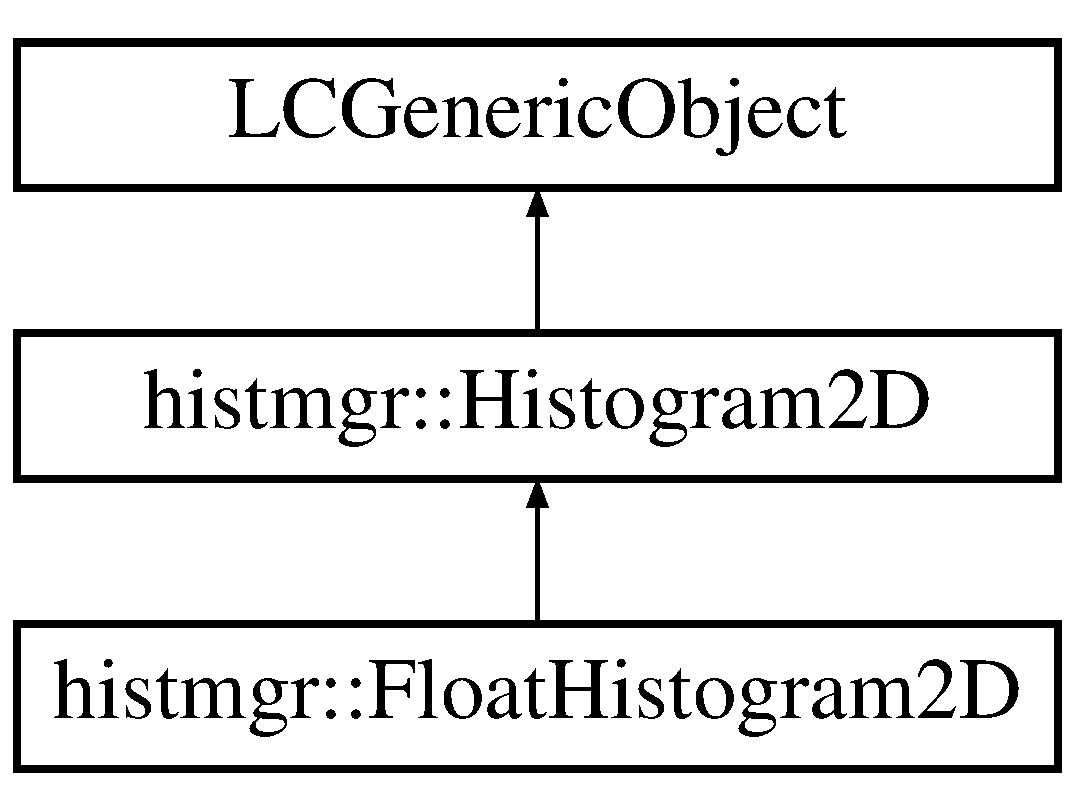
\includegraphics[height=3.000000cm]{classhistmgr_1_1FloatHistogram2D}
\end{center}
\end{figure}
\subsection*{Public Member Functions}
\begin{DoxyCompactItemize}
\item 
{\bf Float\-Histogram2\-D} (U\-Int\-\_\-t {\bf id}, const {\bf Hist\-Par} \&binning\-\_\-x, const {\bf Hist\-Par} \&binning\-\_\-y)
\begin{DoxyCompactList}\small\item\em Create a histogram with a certain binning. \end{DoxyCompactList}\item 
{\bfseries Float\-Histogram2\-D} (lcio\-::\-L\-C\-Object $\ast$a\-\_\-obj)\label{classhistmgr_1_1FloatHistogram2D_ab0dea4b3d379cdb854036719674e71d4}

\item 
{\bfseries Float\-Histogram2\-D} (const {\bf Float\-Histogram2\-D} \&a)\label{classhistmgr_1_1FloatHistogram2D_a68f0f15e037cb32f3d77d6f0984ee3b4}

\item 
void {\bf fill} (Float\-\_\-t value\-\_\-x, Float\-\_\-t value\-\_\-y, Float\-\_\-t weight=1.)\label{classhistmgr_1_1FloatHistogram2D_aa817630a68b7456960a13d984032fce6}

\begin{DoxyCompactList}\small\item\em fill a value into the histogram \end{DoxyCompactList}\item 
void {\bf reset} ()\label{classhistmgr_1_1FloatHistogram2D_ad3fdcad04762ab70fa346e23d7190b97}

\begin{DoxyCompactList}\small\item\em reset the histograms and the number of entries \end{DoxyCompactList}\item 
U\-Int\-\_\-t {\bf bin\-Index} (U\-Int\-\_\-t binx\-\_\-i, U\-Int\-\_\-t biny\-\_\-i) const \label{classhistmgr_1_1FloatHistogram2D_a220db5ab33a4a99a3c1cef4a20b0906c}

\begin{DoxyCompactList}\small\item\em Get the 1d bin index. \end{DoxyCompactList}\item 
void {\bf add\-To\-Bin\-Content} (U\-Int\-\_\-t bin\-\_\-index, Float\-\_\-t value)\label{classhistmgr_1_1FloatHistogram2D_a15daa23f7a152fa7b66aa9615aaa5178}

\begin{DoxyCompactList}\small\item\em manipulate a histogram bin \end{DoxyCompactList}\item 
void {\bf set\-Bin\-Content} (U\-Int\-\_\-t bin\-\_\-index, Float\-\_\-t value)\label{classhistmgr_1_1FloatHistogram2D_ae32ecb4a2dbe9af82e2d9deae0c27ae9}

\begin{DoxyCompactList}\small\item\em manipulate a histogram bin \end{DoxyCompactList}\item 
Float\-\_\-t {\bfseries bin\-Content} (U\-Int\-\_\-t bin\-\_\-index) const \label{classhistmgr_1_1FloatHistogram2D_a49f9dd18dc961e95f62911da156bbc9e}

\item 
Float\-\_\-t {\bfseries x\-Overflow} (U\-Int\-\_\-t biny\-\_\-i) const \label{classhistmgr_1_1FloatHistogram2D_a84ee60b090e66f1a1839f73543284ad2}

\item 
Float\-\_\-t {\bfseries x\-Underflow} (U\-Int\-\_\-t biny\-\_\-i) const \label{classhistmgr_1_1FloatHistogram2D_abc8e206e2cac237b73663320202bb573}

\item 
Float\-\_\-t {\bfseries y\-Overflow} (U\-Int\-\_\-t binx\-\_\-i) const \label{classhistmgr_1_1FloatHistogram2D_ab3951011e9cf17698a7b3cc5c766446f}

\item 
Float\-\_\-t {\bfseries y\-Underflow} (U\-Int\-\_\-t binx\-\_\-i) const \label{classhistmgr_1_1FloatHistogram2D_aa2267579329064792b162fe320881d42}

\item 
Float\-\_\-t {\bfseries x\-Underflow} () const \label{classhistmgr_1_1FloatHistogram2D_a756024a8658045e2157123e7c4cb3889}

\item 
Float\-\_\-t {\bfseries x\-Overflow} () const \label{classhistmgr_1_1FloatHistogram2D_aa0f77dee0d0554a892ef241ade373e07}

\item 
Float\-\_\-t {\bfseries y\-Underflow} () const \label{classhistmgr_1_1FloatHistogram2D_a9615ca79f363ce43a4283a57b2f93bb9}

\item 
Float\-\_\-t {\bfseries y\-Overflow} () const \label{classhistmgr_1_1FloatHistogram2D_af1610406b9e3914576f3643158237dfa}

\item 
Float\-\_\-t {\bfseries x\-Mean} () const \label{classhistmgr_1_1FloatHistogram2D_a7942a45e5b0dd5e353a0d58b62b8de5c}

\item 
Float\-\_\-t {\bf x\-Rms} (bool natural=false) const 
\begin{DoxyCompactList}\small\item\em Root mean square as defined by R\-O\-O\-T. \end{DoxyCompactList}\item 
Float\-\_\-t {\bf x\-Variance} () const 
\begin{DoxyCompactList}\small\item\em Variance. \end{DoxyCompactList}\item 
Float\-\_\-t {\bfseries y\-Mean} () const \label{classhistmgr_1_1FloatHistogram2D_a10414e7c9ad34612626fd74572f8add9}

\item 
Float\-\_\-t {\bf y\-Rms} (bool natural=false) const 
\begin{DoxyCompactList}\small\item\em Root mean square as defined by R\-O\-O\-T. \end{DoxyCompactList}\item 
Float\-\_\-t {\bf y\-Variance} () const 
\begin{DoxyCompactList}\small\item\em Variance. \end{DoxyCompactList}\item 
Double\-\_\-t {\bf integral} (U\-Int\-\_\-t x0\-\_\-i, U\-Int\-\_\-t x1\-\_\-i, U\-Int\-\_\-t y0\-\_\-i, U\-Int\-\_\-t y1\-\_\-i) const 
\begin{DoxyCompactList}\small\item\em sum contents of bins within the given range \end{DoxyCompactList}\item 
lcio\-::\-L\-C\-Object $\ast$ {\bfseries clone} () const \label{classhistmgr_1_1FloatHistogram2D_a3d2ff7763edb2ad062006f7170a32285}

\end{DoxyCompactItemize}
\subsection*{Private Member Functions}
\begin{DoxyCompactItemize}
\item 
U\-Int\-\_\-t {\bfseries n\-X\-Bins\-Total} () const \label{classhistmgr_1_1FloatHistogram2D_af5a817d2d34a4ee5ecde6dc84b4d5996}

\item 
U\-Int\-\_\-t {\bfseries n\-Bins\-Total} () const \label{classhistmgr_1_1FloatHistogram2D_a378ba87874ae6a6d6a2eefc558d3bb7e}

\end{DoxyCompactItemize}
\subsection*{Additional Inherited Members}


\subsection{Detailed Description}
A 1-\/dimensional histogram using float values for the bins. 

Definition at line 12 of file Float\-Histogram2\-D.\-hh.



\subsection{Constructor \& Destructor Documentation}
\index{histmgr\-::\-Float\-Histogram2\-D@{histmgr\-::\-Float\-Histogram2\-D}!Float\-Histogram2\-D@{Float\-Histogram2\-D}}
\index{Float\-Histogram2\-D@{Float\-Histogram2\-D}!histmgr::FloatHistogram2D@{histmgr\-::\-Float\-Histogram2\-D}}
\subsubsection[{Float\-Histogram2\-D}]{\setlength{\rightskip}{0pt plus 5cm}histmgr\-::\-Float\-Histogram2\-D\-::\-Float\-Histogram2\-D (
\begin{DoxyParamCaption}
\item[{U\-Int\-\_\-t}]{id, }
\item[{const {\bf Hist\-Par} \&}]{binning\-\_\-x, }
\item[{const {\bf Hist\-Par} \&}]{binning\-\_\-y}
\end{DoxyParamCaption}
)}\label{classhistmgr_1_1FloatHistogram2D_a2c53fd92a0a2ffa78589ff109acd1b4b}


Create a histogram with a certain binning. 


\begin{DoxyParams}{Parameters}
{\em id} & a unique histogram I\-D, \\
\hline
{\em binning\-\_\-x} & number of bins and range of the axis \\
\hline
{\em binning\-\_\-y} & number of bins and range of the axis \\
\hline
\end{DoxyParams}
\begin{DoxyRefDesc}{Todo}
\item[{\bf Todo}]a name would be better than an I\-D but a string can not be easily stored in an L\-C\-Generic\-Object \end{DoxyRefDesc}


Definition at line 8 of file Float\-Histogram2\-D.\-cc.



References Hist\-Par\-::n\-Bins(), and reset().



\subsection{Member Function Documentation}
\index{histmgr\-::\-Float\-Histogram2\-D@{histmgr\-::\-Float\-Histogram2\-D}!integral@{integral}}
\index{integral@{integral}!histmgr::FloatHistogram2D@{histmgr\-::\-Float\-Histogram2\-D}}
\subsubsection[{integral}]{\setlength{\rightskip}{0pt plus 5cm}Double\-\_\-t histmgr\-::\-Float\-Histogram2\-D\-::integral (
\begin{DoxyParamCaption}
\item[{U\-Int\-\_\-t}]{x0\-\_\-i, }
\item[{U\-Int\-\_\-t}]{x1\-\_\-i, }
\item[{U\-Int\-\_\-t}]{y0\-\_\-i, }
\item[{U\-Int\-\_\-t}]{y1\-\_\-i}
\end{DoxyParamCaption}
) const}\label{classhistmgr_1_1FloatHistogram2D_a32dfa904050e2f247175eb6435147323}


sum contents of bins within the given range 


\begin{DoxyParams}{Parameters}
{\em x0\-\_\-i} & index of the first bin along x \\
\hline
{\em x1\-\_\-i} & index of the last bin (included in the sum) along x \\
\hline
{\em y0\-\_\-i} & index of the first bin along y \\
\hline
{\em y1\-\_\-i} & index of the last bin (included in the sum) along y \\
\hline
\end{DoxyParams}
\begin{DoxyReturn}{Returns}
the sum of the bins 
\end{DoxyReturn}


Definition at line 143 of file Float\-Histogram2\-D.\-cc.

\index{histmgr\-::\-Float\-Histogram2\-D@{histmgr\-::\-Float\-Histogram2\-D}!x\-Rms@{x\-Rms}}
\index{x\-Rms@{x\-Rms}!histmgr::FloatHistogram2D@{histmgr\-::\-Float\-Histogram2\-D}}
\subsubsection[{x\-Rms}]{\setlength{\rightskip}{0pt plus 5cm}Float\-\_\-t histmgr\-::\-Float\-Histogram2\-D\-::x\-Rms (
\begin{DoxyParamCaption}
\item[{bool}]{natural = {\ttfamily false}}
\end{DoxyParamCaption}
) const}\label{classhistmgr_1_1FloatHistogram2D_a59c99c39c90a49a62de6678728ced198}


Root mean square as defined by R\-O\-O\-T. 

divided by n 

Definition at line 65 of file Float\-Histogram2\-D.\-cc.



References bin\-Index().

\index{histmgr\-::\-Float\-Histogram2\-D@{histmgr\-::\-Float\-Histogram2\-D}!x\-Variance@{x\-Variance}}
\index{x\-Variance@{x\-Variance}!histmgr::FloatHistogram2D@{histmgr\-::\-Float\-Histogram2\-D}}
\subsubsection[{x\-Variance}]{\setlength{\rightskip}{0pt plus 5cm}Float\-\_\-t histmgr\-::\-Float\-Histogram2\-D\-::x\-Variance (
\begin{DoxyParamCaption}
{}
\end{DoxyParamCaption}
) const}\label{classhistmgr_1_1FloatHistogram2D_a96200287a4d48feeb7ae60832c760315}


Variance. 

divided by n-\/1 \index{histmgr\-::\-Float\-Histogram2\-D@{histmgr\-::\-Float\-Histogram2\-D}!y\-Rms@{y\-Rms}}
\index{y\-Rms@{y\-Rms}!histmgr::FloatHistogram2D@{histmgr\-::\-Float\-Histogram2\-D}}
\subsubsection[{y\-Rms}]{\setlength{\rightskip}{0pt plus 5cm}Float\-\_\-t histmgr\-::\-Float\-Histogram2\-D\-::y\-Rms (
\begin{DoxyParamCaption}
\item[{bool}]{natural = {\ttfamily false}}
\end{DoxyParamCaption}
) const}\label{classhistmgr_1_1FloatHistogram2D_a44b5d22fb5fe27a9bac978cac174201a}


Root mean square as defined by R\-O\-O\-T. 

divided by n 

Definition at line 115 of file Float\-Histogram2\-D.\-cc.



References bin\-Index().

\index{histmgr\-::\-Float\-Histogram2\-D@{histmgr\-::\-Float\-Histogram2\-D}!y\-Variance@{y\-Variance}}
\index{y\-Variance@{y\-Variance}!histmgr::FloatHistogram2D@{histmgr\-::\-Float\-Histogram2\-D}}
\subsubsection[{y\-Variance}]{\setlength{\rightskip}{0pt plus 5cm}Float\-\_\-t histmgr\-::\-Float\-Histogram2\-D\-::y\-Variance (
\begin{DoxyParamCaption}
{}
\end{DoxyParamCaption}
) const}\label{classhistmgr_1_1FloatHistogram2D_a35e14860e0bd3e2b0370419122f43554}


Variance. 

divided by n-\/1 

The documentation for this class was generated from the following files\-:\begin{DoxyCompactItemize}
\item 
Float\-Histogram2\-D.\-hh\item 
Float\-Histogram2\-D.\-cc\end{DoxyCompactItemize}

\section{histmgr\-:\-:Graph\-Collection\-\_\-t Class Reference}
\label{classhistmgr_1_1GraphCollection__t}\index{histmgr\-::\-Graph\-Collection\-\_\-t@{histmgr\-::\-Graph\-Collection\-\_\-t}}


Light wrapper around a L\-C\-Collection to facilitate the handling of collections of graphs.  




{\ttfamily \#include $<$Graph\-Collection\-\_\-t.\-hh$>$}

Inheritance diagram for histmgr\-:\-:Graph\-Collection\-\_\-t\-:\begin{figure}[H]
\begin{center}
\leavevmode
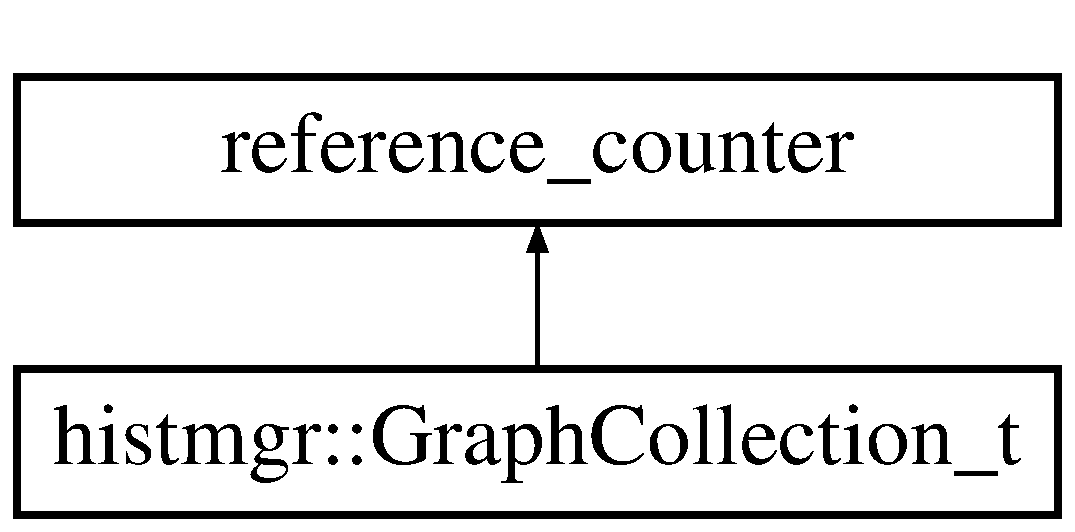
\includegraphics[height=2.000000cm]{classhistmgr_1_1GraphCollection__t}
\end{center}
\end{figure}
\subsection*{Public Member Functions}
\begin{DoxyCompactItemize}
\item 
{\bfseries Graph\-Collection\-\_\-t} (const std\-::string \&collection\-\_\-name, unsigned int n\-\_\-graphs, const E\-V\-E\-N\-T\-::\-String\-Vec \&type\-\_\-names, unsigned int n\-\_\-expected\-\_\-values, const E\-V\-E\-N\-T\-::\-String\-Vec \&opt\-\_\-major\-\_\-names) noexcept(false)\label{classhistmgr_1_1GraphCollection__t_a76a01f4cea149390f87f3e6385659a72}

\item 
{\bfseries Graph\-Collection\-\_\-t} (const std\-::string \&collection\-\_\-name, const std\-::vector$<$ unsigned int $>$ \&n\-\_\-graphs, const std\-::vector$<$ std\-::string $>$ \&type\-\_\-names, unsigned int n\-\_\-expected\-\_\-values, const std\-::vector$<$ std\-::string $>$ \&opt\-\_\-major\-\_\-names) noexcept(false)\label{classhistmgr_1_1GraphCollection__t_ae4359affd7572ee7f4aec202d9275a67}

\item 
{\bf Graph\-Collection\-\_\-t} (lcio\-::\-L\-C\-Collection $\ast$graphs, lcio\-::\-Int\-Vec $\ast$indices)
\item 
{\bf Graph\-Collection\-\_\-t} (lcio\-::\-L\-C\-Collection $\ast$graphs)
\begin{DoxyCompactList}\small\item\em Create a histogram collection from lcio collection. \end{DoxyCompactList}\item 
{\bf Graph\-Collection\-\_\-t} (const {\bf Graph\-Collection\-\_\-t} \&a)\label{classhistmgr_1_1GraphCollection__t_a8beca08f62d11c86c76e861678e0a256}

\begin{DoxyCompactList}\small\item\em copy constructor. \end{DoxyCompactList}\item 
void {\bf delete\-Collection} ()\label{classhistmgr_1_1GraphCollection__t_a9e80261bb734fb1f63480aee46764ffe}

\begin{DoxyCompactList}\small\item\em delete the histogram collection and the index array This method exists instead of a destrctor to prevent copying the arrays (F\-I\-X\-M\-E) \end{DoxyCompactList}\item 
void {\bfseries delete\-Shared\-Storage} ()\label{classhistmgr_1_1GraphCollection__t_aa3c1de2ff8e58f55dd92b68ce42d0535}

\item 
lcio\-::\-L\-C\-Collection $\ast$ {\bf collection} ()
\begin{DoxyCompactList}\small\item\em get the unique group id \end{DoxyCompactList}\item 
const lcio\-::\-L\-C\-Collection $\ast$ {\bf collection} () const 
\begin{DoxyCompactList}\small\item\em get the collection of graphs (read only). \end{DoxyCompactList}\item 
unsigned int {\bf n} () const 
\begin{DoxyCompactList}\small\item\em Get the number of graphs. \end{DoxyCompactList}\item 
bool {\bf is2\-D} () const 
\begin{DoxyCompactList}\small\item\em Check whether the graph collection contains more than one graph group. \end{DoxyCompactList}\item 
unsigned int {\bfseries n\-Types} () const \label{classhistmgr_1_1GraphCollection__t_aa2092b41bf92f55d260e754ff26e48f2}

\item 
unsigned int {\bf n\-Major} () const 
\begin{DoxyCompactList}\small\item\em Get the number of major indices. \end{DoxyCompactList}\item 
unsigned int {\bf n\-Minor} (unsigned int major\-\_\-index) const 
\begin{DoxyCompactList}\small\item\em Get the number of elements for the collection slice addressed by the given major index. \end{DoxyCompactList}\item 
{\bf Graph\-Collection\-\_\-t} (const std\-::string \&collection\-\_\-name, unsigned int n\-\_\-graphs, const E\-V\-E\-N\-T\-::\-String\-Vec \&type\-\_\-names, unsigned int n\-\_\-expected\-\_\-values, const E\-V\-E\-N\-T\-::\-String\-Vec \&opt\-\_\-major\-\_\-names, bool may\-\_\-overwrite=false) noexcept(false)
\begin{DoxyCompactList}\small\item\em Create a collection of graphs. \end{DoxyCompactList}\item 
{\bf Graph\-Collection\-\_\-t} (const std\-::string \&collection\-\_\-name, const std\-::vector$<$ int $>$ \&n\-\_\-graphs, const std\-::vector$<$ std\-::string $>$ \&type\-\_\-names, unsigned int n\-\_\-expected\-\_\-values, const std\-::vector$<$ std\-::string $>$ \&opt\-\_\-major\-\_\-names, bool may\-\_\-overwrite=false) noexcept(false)
\begin{DoxyCompactList}\small\item\em Create a 2\-D collection of graphs. \end{DoxyCompactList}\item 
std\-::string \& {\bf get\-Major\-Name} (unsigned int major\-\_\-index, unsigned int type\-\_\-index) const 
\begin{DoxyCompactList}\small\item\em Get the name of the graph group addressed by the major index. \end{DoxyCompactList}\item 
std\-::string \& {\bf get\-Name} (unsigned int major\-\_\-index, unsigned int minor\-\_\-index, unsigned int type\-\_\-index) const 
\begin{DoxyCompactList}\small\item\em Get the full name of the graph which is part of a specfic graph group addressed by the major index. \end{DoxyCompactList}\item 
std\-::string \& {\bf get\-Name} (unsigned int index, unsigned int type\-\_\-index) const 
\begin{DoxyCompactList}\small\item\em Get the full name of the graph addressed by the index. \end{DoxyCompactList}\item 
unsigned int {\bf append\-X\-Value} (double x\-\_\-value)
\begin{DoxyCompactList}\small\item\em Set the common x value of all the graphs of the graph collection. \end{DoxyCompactList}\item 
void {\bf set\-Y\-Value} (unsigned int major\-\_\-index, unsigned int minor\-\_\-index, unsigned int type\-\_\-index, unsigned int value\-\_\-index, float a\-\_\-value)\label{classhistmgr_1_1GraphCollection__t_a2d86a21418a91537e8cb831673b4e88b}

\begin{DoxyCompactList}\small\item\em Set the y-\/value of the adddressed graph. \end{DoxyCompactList}\item 
void {\bf set\-Y\-Value} (unsigned int index, unsigned int type\-\_\-index, unsigned int value\-\_\-index, float a\-\_\-value)\label{classhistmgr_1_1GraphCollection__t_afa630f68afc52b4f115fe35e1c652119}

\begin{DoxyCompactList}\small\item\em Set the y-\/value of the adddressed graph. \end{DoxyCompactList}\item 
float {\bf get\-Y\-Value} (unsigned int index, unsigned int type\-\_\-index, unsigned int value\-\_\-index) const \label{classhistmgr_1_1GraphCollection__t_aa897bd01a3c31af0e8b82dbef6b57271}

\begin{DoxyCompactList}\small\item\em Get the y-\/value of the adddressed graph. \end{DoxyCompactList}\item 
float {\bf get\-Y\-Value} (unsigned int major\-\_\-index, unsigned int minor\-\_\-index, unsigned int type\-\_\-index, unsigned int value\-\_\-index) const \label{classhistmgr_1_1GraphCollection__t_a16f16887fc54666fca9fb47c8d45a6d0}

\begin{DoxyCompactList}\small\item\em Get the y-\/value of the adddressed graph. \end{DoxyCompactList}\item 
double {\bf get\-X\-Value} (unsigned int index, unsigned int value\-\_\-index) const \label{classhistmgr_1_1GraphCollection__t_a7dd9e9ac73e5e5ba7bf9f2786a73af0b}

\begin{DoxyCompactList}\small\item\em Get the x-\/value of the adddressed graph. \end{DoxyCompactList}\item 
const std\-::string \& {\bf get\-Name} (unsigned int major\-\_\-index) const 
\begin{DoxyCompactList}\small\item\em Get the name of the specified element of the graph collection. \end{DoxyCompactList}\item 
const std\-::string \& {\bf get\-Type\-Name} (unsigned int type\-\_\-index) const 
\begin{DoxyCompactList}\small\item\em Get the addressed type name. \end{DoxyCompactList}\end{DoxyCompactItemize}
\subsection*{Static Public Attributes}
\begin{DoxyCompactItemize}
\item 
static const std\-::string {\bfseries \-\_\-\-\_\-color\-Parameter\-Name}\label{classhistmgr_1_1GraphCollection__t_a1934a2578324612aa48e561e45058694}

\item 
static const std\-::string {\bfseries \-\_\-\-\_\-width\-Parameter\-Name}\label{classhistmgr_1_1GraphCollection__t_ac0f6932a278f313baffc9939f4cb06b3}

\item 
static const std\-::string {\bfseries \-\_\-\-\_\-style\-Parameter\-Name}\label{classhistmgr_1_1GraphCollection__t_acd025c2ba443992253384db6a7d17a8e}

\item 
static const std\-::string {\bfseries \-\_\-\-\_\-major\-Color\-Parameter\-Name}\label{classhistmgr_1_1GraphCollection__t_a8dfd0bff85a2211a1e7090aa43506c4d}

\end{DoxyCompactItemize}
\subsection*{Protected Member Functions}
\begin{DoxyCompactItemize}
\item 
unsigned int {\bf append\-Float\-Value} (unsigned int full\-\_\-index, float a\-\_\-value)\label{classhistmgr_1_1GraphCollection__t_a28fd99da38b507b16d24dff9e7b6b1eb}

\begin{DoxyCompactList}\small\item\em append a new value to the addressed graph, \end{DoxyCompactList}\item 
unsigned int {\bf append\-Value} (unsigned int full\-\_\-index, double a\-\_\-value)\label{classhistmgr_1_1GraphCollection__t_a28ab4fba47b05ef353dd81c76ee4b1b3}

\begin{DoxyCompactList}\small\item\em append a new value to the addressed graph, \end{DoxyCompactList}\item 
void {\bf set\-Float\-Value} (unsigned int full\-\_\-index, unsigned int value\-\_\-index, float a\-\_\-value)\label{classhistmgr_1_1GraphCollection__t_a2768ffebabe6eb28b985a622697d263e}

\begin{DoxyCompactList}\small\item\em set a value of the addressed graph, \end{DoxyCompactList}\item 
void {\bf set\-Value} (unsigned int full\-\_\-index, unsigned int value\-\_\-index, float a\-\_\-value)\label{classhistmgr_1_1GraphCollection__t_afe1fbbf9ce02123a6f0d13af1ccf48ab}

\begin{DoxyCompactList}\small\item\em set a value of the addressed graph, \end{DoxyCompactList}\item 
double {\bf get\-Value} (unsigned int full\-\_\-index, unsigned int value\-\_\-index) const \label{classhistmgr_1_1GraphCollection__t_a85dd0752c73cfdd78909e1e3e7e55cbf}

\begin{DoxyCompactList}\small\item\em set a value of the addressed graph, \end{DoxyCompactList}\item 
double {\bf get\-Float\-Value} (unsigned int full\-\_\-index, unsigned int value\-\_\-index) const \label{classhistmgr_1_1GraphCollection__t_a55ab641e3179a97e4d609deea290eb37}

\begin{DoxyCompactList}\small\item\em set a value of the addressed graph, \end{DoxyCompactList}\item 
void {\bf add\-To\-Float\-Value} (unsigned int full\-\_\-index, unsigned int value\-\_\-index, float a\-\_\-value)\label{classhistmgr_1_1GraphCollection__t_a5e747206119488483b0b46c11342dace}

\begin{DoxyCompactList}\small\item\em Add the given value to a certain value of the addressed graph. \end{DoxyCompactList}\item 
unsigned int {\bf get\-Index} (unsigned int major\-\_\-index, unsigned int minor\-\_\-index, unsigned int type\-\_\-index) const \label{classhistmgr_1_1GraphCollection__t_ae56f52a4ec2a8188b7a3be59c2f90090}

\begin{DoxyCompactList}\small\item\em Calculate the full graph index in case of 2d graph groups. \end{DoxyCompactList}\item 
unsigned int {\bf get\-Index} (unsigned int index, unsigned int type\-\_\-index) const \label{classhistmgr_1_1GraphCollection__t_a6babd769d8db88965939660a221ea4b9}

\begin{DoxyCompactList}\small\item\em Calculate the full graph index in case of a flat graph group. \end{DoxyCompactList}\item 
E\-V\-E\-N\-T\-::\-L\-C\-Generic\-Object $\ast$ {\bfseries get\-X\-Array} ()\label{classhistmgr_1_1GraphCollection__t_a2dbf7fc55d252547d24cbac999f0f55e}

\item 
E\-V\-E\-N\-T\-::\-L\-C\-Generic\-Object $\ast$ {\bfseries get\-Array} (unsigned int full\-\_\-index)\label{classhistmgr_1_1GraphCollection__t_a3e2a4928f2ff0d2249771d76be53c82e}

\end{DoxyCompactItemize}
\subsection*{Static Protected Attributes}
\begin{DoxyCompactItemize}
\item 
static const std\-::string {\bfseries \-\_\-\-\_\-graph\-Name\-Parameter\-Name}\label{classhistmgr_1_1GraphCollection__t_a1c88428395aa2448fa920b2fd3fc21c1}

\end{DoxyCompactItemize}
\subsection*{Private Member Functions}
\begin{DoxyCompactItemize}
\item 
void {\bf copy\-Names} () const 
\begin{DoxyCompactList}\small\item\em Assignment operation which deletes the old collections. \end{DoxyCompactList}\end{DoxyCompactItemize}
\subsection*{Private Attributes}
\begin{DoxyCompactItemize}
\item 
lcio\-::\-L\-C\-Collection $\ast$ {\bf \-\_\-graph\-Col}\label{classhistmgr_1_1GraphCollection__t_a1196d28c374dfd4e4fdd291542b392f2}

\begin{DoxyCompactList}\small\item\em the histogram collection \end{DoxyCompactList}\item 
unsigned int {\bf \-\_\-n\-Graphs}\label{classhistmgr_1_1GraphCollection__t_ab839badb20a05434321be1bf9ff36831}

\begin{DoxyCompactList}\small\item\em the number of graphs \end{DoxyCompactList}\item 
lcio\-::\-Int\-Vec $\ast$ {\bf \-\_\-major\-Index}
\begin{DoxyCompactList}\small\item\em optional list of offset to form a two dimensional array out of the list. \end{DoxyCompactList}\item 
unsigned int {\bf \-\_\-n\-Types}
\begin{DoxyCompactList}\small\item\em number of types. \end{DoxyCompactList}\item 
lcio\-::\-String\-Vec {\bf \-\_\-type\-Name\-List}
\begin{DoxyCompactList}\small\item\em A vector which contains one name for all graphs of the collection or a name for each element (this list is only filled if a names are accessed). \end{DoxyCompactList}\item 
lcio\-::\-String\-Vec {\bf \-\_\-name\-List}
\begin{DoxyCompactList}\small\item\em A vector which contains one name for all graphs of the collection or a name for each element. \end{DoxyCompactList}\end{DoxyCompactItemize}
\subsection*{Static Private Attributes}
\begin{DoxyCompactItemize}
\item 
static const std\-::string {\bfseries \-\_\-\-\_\-major\-Index\-Parameter\-Name}\label{classhistmgr_1_1GraphCollection__t_adaba3b377fc3c74c4b34fcae6b032849}

\item 
static const std\-::string {\bfseries \-\_\-\-\_\-type\-Name\-Parameter\-Name}\label{classhistmgr_1_1GraphCollection__t_aab8c996982d62a8eab7cd537394a07b1}

\item 
static const std\-::string {\bfseries \-\_\-\-\_\-default\-Graph\-Name}\label{classhistmgr_1_1GraphCollection__t_ad7c3d4148ee7dcfbab8485fb3e7872c0}

\end{DoxyCompactItemize}
\subsection*{Friends}
\begin{DoxyCompactItemize}
\item 
class {\bfseries Hist\-Mgr}\label{classhistmgr_1_1GraphCollection__t_a3cc85db784d7651390e41024125eb3a0}

\end{DoxyCompactItemize}


\subsection{Detailed Description}
Light wrapper around a L\-C\-Collection to facilitate the handling of collections of graphs. 

All the graphs of the collection share the same x values. The wrapper supports 1 or 2 dimensional collections of graphs. Where each graph collection is composed of several graph groups and each graph group contains a fixed set of graphs of different types. More correctly the collection has a 2 dimensional or 3d diemensional structure. 

Definition at line 27 of file Graph\-Collection\-\_\-t.\-hh.



\subsection{Constructor \& Destructor Documentation}
\index{histmgr\-::\-Graph\-Collection\-\_\-t@{histmgr\-::\-Graph\-Collection\-\_\-t}!Graph\-Collection\-\_\-t@{Graph\-Collection\-\_\-t}}
\index{Graph\-Collection\-\_\-t@{Graph\-Collection\-\_\-t}!histmgr::GraphCollection_t@{histmgr\-::\-Graph\-Collection\-\_\-t}}
\subsubsection[{Graph\-Collection\-\_\-t}]{\setlength{\rightskip}{0pt plus 5cm}histmgr\-::\-Graph\-Collection\-\_\-t\-::\-Graph\-Collection\-\_\-t (
\begin{DoxyParamCaption}
\item[{lcio\-::\-L\-C\-Collection $\ast$}]{graphs, }
\item[{lcio\-::\-Int\-Vec $\ast$}]{indices}
\end{DoxyParamCaption}
)}\label{classhistmgr_1_1GraphCollection__t_a740ae9b62df86330c2734fdf061b119a}

\begin{DoxyParams}{Parameters}
{\em graphs} & the linearised one or two dimensional collection of graphs \\
\hline
{\em indices} & optional list of indicies used to give two dimensional access to the histogram list. for each possible index of the first dimension is needed which contains the offset in the list. The second index is added to this offset. \\
\hline
\end{DoxyParams}


Definition at line 124 of file Graph\-Collection\-\_\-t.\-cc.



References \-\_\-graph\-Col, \-\_\-major\-Index, \-\_\-n\-Graphs, and \-\_\-n\-Types.

\index{histmgr\-::\-Graph\-Collection\-\_\-t@{histmgr\-::\-Graph\-Collection\-\_\-t}!Graph\-Collection\-\_\-t@{Graph\-Collection\-\_\-t}}
\index{Graph\-Collection\-\_\-t@{Graph\-Collection\-\_\-t}!histmgr::GraphCollection_t@{histmgr\-::\-Graph\-Collection\-\_\-t}}
\subsubsection[{Graph\-Collection\-\_\-t}]{\setlength{\rightskip}{0pt plus 5cm}histmgr\-::\-Graph\-Collection\-\_\-t\-::\-Graph\-Collection\-\_\-t (
\begin{DoxyParamCaption}
\item[{lcio\-::\-L\-C\-Collection $\ast$}]{graphs}
\end{DoxyParamCaption}
)}\label{classhistmgr_1_1GraphCollection__t_a1f8d2f420b8735f4ff9ae71d976f6622}


Create a histogram collection from lcio collection. 


\begin{DoxyParams}{Parameters}
{\em graphs} & the linearised one or two dimensional collection of graphs (two dimensional collections have the collection parameter \char`\"{}major\char`\"{}). The method does not verify whether the lcio collection really is a histogram collection. However, if the collection has the parameter \char`\"{}major\char`\"{} it creates an index vector (costly operation) assuming that it is a 2d array instead of a 1d array(i.\-e. collection). The unique group id remains undedfined since it is not stored in the lcio collection. \\
\hline
\end{DoxyParams}


Definition at line 151 of file Graph\-Collection\-\_\-t.\-cc.



References \-\_\-graph\-Col, \-\_\-major\-Index, \-\_\-n\-Graphs, and \-\_\-n\-Types.

\index{histmgr\-::\-Graph\-Collection\-\_\-t@{histmgr\-::\-Graph\-Collection\-\_\-t}!Graph\-Collection\-\_\-t@{Graph\-Collection\-\_\-t}}
\index{Graph\-Collection\-\_\-t@{Graph\-Collection\-\_\-t}!histmgr::GraphCollection_t@{histmgr\-::\-Graph\-Collection\-\_\-t}}
\subsubsection[{Graph\-Collection\-\_\-t}]{\setlength{\rightskip}{0pt plus 5cm}histmgr\-::\-Graph\-Collection\-\_\-t\-::\-Graph\-Collection\-\_\-t (
\begin{DoxyParamCaption}
\item[{const std\-::string \&}]{collection\-\_\-name, }
\item[{unsigned int}]{n\-\_\-graphs, }
\item[{const E\-V\-E\-N\-T\-::\-String\-Vec \&}]{type\-\_\-names, }
\item[{unsigned int}]{n\-\_\-expected\-\_\-values, }
\item[{const E\-V\-E\-N\-T\-::\-String\-Vec \&}]{opt\-\_\-major\-\_\-names, }
\item[{bool}]{may\-\_\-overwrite = {\ttfamily false}}
\end{DoxyParamCaption}
)\hspace{0.3cm}{\ttfamily [noexcept]}}\label{classhistmgr_1_1GraphCollection__t_abf3f0a07e3feaabb90dd54c9a7ad0b74}


Create a collection of graphs. 

Where for each element the given number of graph types is created. 

Definition at line 17 of file Graph\-Collection\-\_\-t.\-cc.

\index{histmgr\-::\-Graph\-Collection\-\_\-t@{histmgr\-::\-Graph\-Collection\-\_\-t}!Graph\-Collection\-\_\-t@{Graph\-Collection\-\_\-t}}
\index{Graph\-Collection\-\_\-t@{Graph\-Collection\-\_\-t}!histmgr::GraphCollection_t@{histmgr\-::\-Graph\-Collection\-\_\-t}}
\subsubsection[{Graph\-Collection\-\_\-t}]{\setlength{\rightskip}{0pt plus 5cm}histmgr\-::\-Graph\-Collection\-\_\-t\-::\-Graph\-Collection\-\_\-t (
\begin{DoxyParamCaption}
\item[{const std\-::string \&}]{collection\-\_\-name, }
\item[{const std\-::vector$<$ int $>$ \&}]{n\-\_\-graphs, }
\item[{const std\-::vector$<$ std\-::string $>$ \&}]{type\-\_\-names, }
\item[{unsigned int}]{n\-\_\-expected\-\_\-values, }
\item[{const std\-::vector$<$ std\-::string $>$ \&}]{opt\-\_\-major\-\_\-names, }
\item[{bool}]{may\-\_\-overwrite = {\ttfamily false}}
\end{DoxyParamCaption}
)\hspace{0.3cm}{\ttfamily [noexcept]}}\label{classhistmgr_1_1GraphCollection__t_ab727f95866b9c1a91e869fbc79baf8ba}


Create a 2\-D collection of graphs. 

Where for each element of the 2 dimensional collection, the not only a single but for each graph type one.. 

Definition at line 63 of file Graph\-Collection\-\_\-t.\-cc.



\subsection{Member Function Documentation}
\index{histmgr\-::\-Graph\-Collection\-\_\-t@{histmgr\-::\-Graph\-Collection\-\_\-t}!append\-X\-Value@{append\-X\-Value}}
\index{append\-X\-Value@{append\-X\-Value}!histmgr::GraphCollection_t@{histmgr\-::\-Graph\-Collection\-\_\-t}}
\subsubsection[{append\-X\-Value}]{\setlength{\rightskip}{0pt plus 5cm}unsigned int histmgr\-::\-Graph\-Collection\-\_\-t\-::append\-X\-Value (
\begin{DoxyParamCaption}
\item[{double}]{x\-\_\-value}
\end{DoxyParamCaption}
)\hspace{0.3cm}{\ttfamily [inline]}}\label{classhistmgr_1_1GraphCollection__t_ae9c83cf79211ef808f75343c7c3c3c3d}


Set the common x value of all the graphs of the graph collection. 

\begin{DoxyReturn}{Returns}
the index of the new value which can be used to set the corresponding values in all the other graphs. 
\end{DoxyReturn}


Definition at line 204 of file Graph\-Collection\-\_\-t.\-hh.



References append\-Value().



Referenced by C\-A\-L\-I\-C\-E\-::\-Average\-History\-Graphs\-::process\-Event().

\index{histmgr\-::\-Graph\-Collection\-\_\-t@{histmgr\-::\-Graph\-Collection\-\_\-t}!collection@{collection}}
\index{collection@{collection}!histmgr::GraphCollection_t@{histmgr\-::\-Graph\-Collection\-\_\-t}}
\subsubsection[{collection}]{\setlength{\rightskip}{0pt plus 5cm}lcio\-::\-L\-C\-Collection$\ast$ histmgr\-::\-Graph\-Collection\-\_\-t\-::collection (
\begin{DoxyParamCaption}
{}
\end{DoxyParamCaption}
)\hspace{0.3cm}{\ttfamily [inline]}}\label{classhistmgr_1_1GraphCollection__t_a10bbe40ded94d3664d9eca002986075e}


get the unique group id 

get the collection of graphs. The index array needed for the two dimensional acces is added as a parameter named \char`\"{}major\char`\"{}. 

Definition at line 113 of file Graph\-Collection\-\_\-t.\-hh.



References \-\_\-graph\-Col.

\index{histmgr\-::\-Graph\-Collection\-\_\-t@{histmgr\-::\-Graph\-Collection\-\_\-t}!collection@{collection}}
\index{collection@{collection}!histmgr::GraphCollection_t@{histmgr\-::\-Graph\-Collection\-\_\-t}}
\subsubsection[{collection}]{\setlength{\rightskip}{0pt plus 5cm}const lcio\-::\-L\-C\-Collection$\ast$ histmgr\-::\-Graph\-Collection\-\_\-t\-::collection (
\begin{DoxyParamCaption}
{}
\end{DoxyParamCaption}
) const\hspace{0.3cm}{\ttfamily [inline]}}\label{classhistmgr_1_1GraphCollection__t_ab8754e9146c1fe855d176fe472413cf1}


get the collection of graphs (read only). 

The index array needed for the two dimensional acces is added as a parameter named \char`\"{}major\char`\"{}. 

Definition at line 118 of file Graph\-Collection\-\_\-t.\-hh.



References \-\_\-graph\-Col.

\index{histmgr\-::\-Graph\-Collection\-\_\-t@{histmgr\-::\-Graph\-Collection\-\_\-t}!copy\-Names@{copy\-Names}}
\index{copy\-Names@{copy\-Names}!histmgr::GraphCollection_t@{histmgr\-::\-Graph\-Collection\-\_\-t}}
\subsubsection[{copy\-Names}]{\setlength{\rightskip}{0pt plus 5cm}void histmgr\-::\-Graph\-Collection\-\_\-t\-::copy\-Names (
\begin{DoxyParamCaption}
{}
\end{DoxyParamCaption}
) const\hspace{0.3cm}{\ttfamily [inline]}, {\ttfamily [private]}}\label{classhistmgr_1_1GraphCollection__t_abf045126bb8f97d49b3e07d776c5724a}


Assignment operation which deletes the old collections. 

Copy the names from the collection to an accessible vector. The vector of histogram names is attached as a parameter to the L\-C\-Collection. 

Definition at line 444 of file Graph\-Collection\-\_\-t.\-hh.



References \-\_\-graph\-Col, \-\_\-name\-List, and n\-Major().



Referenced by get\-Name().

\index{histmgr\-::\-Graph\-Collection\-\_\-t@{histmgr\-::\-Graph\-Collection\-\_\-t}!get\-Major\-Name@{get\-Major\-Name}}
\index{get\-Major\-Name@{get\-Major\-Name}!histmgr::GraphCollection_t@{histmgr\-::\-Graph\-Collection\-\_\-t}}
\subsubsection[{get\-Major\-Name}]{\setlength{\rightskip}{0pt plus 5cm}std\-::string\& histmgr\-::\-Graph\-Collection\-\_\-t\-::get\-Major\-Name (
\begin{DoxyParamCaption}
\item[{unsigned int}]{major\-\_\-index, }
\item[{unsigned int}]{type\-\_\-index}
\end{DoxyParamCaption}
) const}\label{classhistmgr_1_1GraphCollection__t_a83cbcc31d10a4ee5ad144dbbab667b28}


Get the name of the graph group addressed by the major index. 

The result is undefined if the graph group is not 2\-D. \index{histmgr\-::\-Graph\-Collection\-\_\-t@{histmgr\-::\-Graph\-Collection\-\_\-t}!get\-Name@{get\-Name}}
\index{get\-Name@{get\-Name}!histmgr::GraphCollection_t@{histmgr\-::\-Graph\-Collection\-\_\-t}}
\subsubsection[{get\-Name}]{\setlength{\rightskip}{0pt plus 5cm}std\-::string\& histmgr\-::\-Graph\-Collection\-\_\-t\-::get\-Name (
\begin{DoxyParamCaption}
\item[{unsigned int}]{major\-\_\-index, }
\item[{unsigned int}]{minor\-\_\-index, }
\item[{unsigned int}]{type\-\_\-index}
\end{DoxyParamCaption}
) const}\label{classhistmgr_1_1GraphCollection__t_a2da46bcaf8e6e11f58b7d0dba88061c8}


Get the full name of the graph which is part of a specfic graph group addressed by the major index. 


\begin{DoxyParams}{Parameters}
{\em major\-\_\-index} & the index of the sub graph group. \\
\hline
{\em minor\-\_\-index} & the index of the graph in the graph group. \\
\hline
{\em type\-\_\-index} & the index of the graph type. \\
\hline
\end{DoxyParams}
\begin{DoxyReturn}{Returns}
the full graph name. The result is undefined if the graph group is not 2\-D. 
\end{DoxyReturn}
\index{histmgr\-::\-Graph\-Collection\-\_\-t@{histmgr\-::\-Graph\-Collection\-\_\-t}!get\-Name@{get\-Name}}
\index{get\-Name@{get\-Name}!histmgr::GraphCollection_t@{histmgr\-::\-Graph\-Collection\-\_\-t}}
\subsubsection[{get\-Name}]{\setlength{\rightskip}{0pt plus 5cm}std\-::string\& histmgr\-::\-Graph\-Collection\-\_\-t\-::get\-Name (
\begin{DoxyParamCaption}
\item[{unsigned int}]{index, }
\item[{unsigned int}]{type\-\_\-index}
\end{DoxyParamCaption}
) const}\label{classhistmgr_1_1GraphCollection__t_a92a1dd0f7dbd265d4fffc81a7fd77ec6}


Get the full name of the graph addressed by the index. 


\begin{DoxyParams}{Parameters}
{\em index} & the index of the graph in the graph group. \\
\hline
{\em type\-\_\-index} & the index of the graph type. \\
\hline
\end{DoxyParams}
\begin{DoxyReturn}{Returns}
the full graph name. The result is undefined if the graph group is not 2\-D. 
\end{DoxyReturn}
\index{histmgr\-::\-Graph\-Collection\-\_\-t@{histmgr\-::\-Graph\-Collection\-\_\-t}!get\-Name@{get\-Name}}
\index{get\-Name@{get\-Name}!histmgr::GraphCollection_t@{histmgr\-::\-Graph\-Collection\-\_\-t}}
\subsubsection[{get\-Name}]{\setlength{\rightskip}{0pt plus 5cm}const std\-::string\& histmgr\-::\-Graph\-Collection\-\_\-t\-::get\-Name (
\begin{DoxyParamCaption}
\item[{unsigned int}]{major\-\_\-index}
\end{DoxyParamCaption}
) const\hspace{0.3cm}{\ttfamily [inline]}}\label{classhistmgr_1_1GraphCollection__t_a89505919c7802e21324986f342afe48e}


Get the name of the specified element of the graph collection. 


\begin{DoxyParams}{Parameters}
{\em major\-\_\-index} & the index of the histogram element or in case of an 2\-D histogram array the major index. \\
\hline
\end{DoxyParams}
\begin{DoxyReturn}{Returns}
a reference to the name. The index must be valid. 
\end{DoxyReturn}


Definition at line 381 of file Graph\-Collection\-\_\-t.\-hh.



References \-\_\-name\-List, and copy\-Names().

\index{histmgr\-::\-Graph\-Collection\-\_\-t@{histmgr\-::\-Graph\-Collection\-\_\-t}!get\-Type\-Name@{get\-Type\-Name}}
\index{get\-Type\-Name@{get\-Type\-Name}!histmgr::GraphCollection_t@{histmgr\-::\-Graph\-Collection\-\_\-t}}
\subsubsection[{get\-Type\-Name}]{\setlength{\rightskip}{0pt plus 5cm}const std\-::string\& histmgr\-::\-Graph\-Collection\-\_\-t\-::get\-Type\-Name (
\begin{DoxyParamCaption}
\item[{unsigned int}]{type\-\_\-index}
\end{DoxyParamCaption}
) const\hspace{0.3cm}{\ttfamily [inline]}}\label{classhistmgr_1_1GraphCollection__t_aec15ce9e41b61e235c0b017d47974a08}


Get the addressed type name. 


\begin{DoxyParams}{Parameters}
{\em type\-\_\-index} & the index of the type. \\
\hline
\end{DoxyParams}
\begin{DoxyReturn}{Returns}
a reference to the type name. The index must be valid. 
\end{DoxyReturn}


Definition at line 397 of file Graph\-Collection\-\_\-t.\-hh.



References \-\_\-graph\-Col, and \-\_\-type\-Name\-List.

\index{histmgr\-::\-Graph\-Collection\-\_\-t@{histmgr\-::\-Graph\-Collection\-\_\-t}!is2\-D@{is2\-D}}
\index{is2\-D@{is2\-D}!histmgr::GraphCollection_t@{histmgr\-::\-Graph\-Collection\-\_\-t}}
\subsubsection[{is2\-D}]{\setlength{\rightskip}{0pt plus 5cm}bool histmgr\-::\-Graph\-Collection\-\_\-t\-::is2\-D (
\begin{DoxyParamCaption}
{}
\end{DoxyParamCaption}
) const\hspace{0.3cm}{\ttfamily [inline]}}\label{classhistmgr_1_1GraphCollection__t_a67af785a9177d9c41e5f7f3251c2d75b}


Check whether the graph collection contains more than one graph group. 

\begin{DoxyReturn}{Returns}
true if the graph collection contains more than one graph group which can be addressed by a major index. 
\end{DoxyReturn}


Definition at line 130 of file Graph\-Collection\-\_\-t.\-hh.



References \-\_\-major\-Index.



Referenced by get\-Index().

\index{histmgr\-::\-Graph\-Collection\-\_\-t@{histmgr\-::\-Graph\-Collection\-\_\-t}!n@{n}}
\index{n@{n}!histmgr::GraphCollection_t@{histmgr\-::\-Graph\-Collection\-\_\-t}}
\subsubsection[{n}]{\setlength{\rightskip}{0pt plus 5cm}unsigned int histmgr\-::\-Graph\-Collection\-\_\-t\-::n (
\begin{DoxyParamCaption}
{}
\end{DoxyParamCaption}
) const\hspace{0.3cm}{\ttfamily [inline]}}\label{classhistmgr_1_1GraphCollection__t_a6ee4913773c2949d5cf3a167038f9a3d}


Get the number of graphs. 

This value does not take into account that for each graph several types are created. 

Definition at line 123 of file Graph\-Collection\-\_\-t.\-hh.



References \-\_\-n\-Graphs.



Referenced by histmgr\-::\-Hist\-Mgr\-::fill\-Histogram\-Collection\-List().

\index{histmgr\-::\-Graph\-Collection\-\_\-t@{histmgr\-::\-Graph\-Collection\-\_\-t}!n\-Major@{n\-Major}}
\index{n\-Major@{n\-Major}!histmgr::GraphCollection_t@{histmgr\-::\-Graph\-Collection\-\_\-t}}
\subsubsection[{n\-Major}]{\setlength{\rightskip}{0pt plus 5cm}unsigned int histmgr\-::\-Graph\-Collection\-\_\-t\-::n\-Major (
\begin{DoxyParamCaption}
{}
\end{DoxyParamCaption}
) const\hspace{0.3cm}{\ttfamily [inline]}}\label{classhistmgr_1_1GraphCollection__t_ac28f1f78b0326c5e91c40a8d74bb0b49}


Get the number of major indices. 

The collection is sliced in n\-Major slices each having n\-Minor(major\-\_\-index) elements. 

Definition at line 144 of file Graph\-Collection\-\_\-t.\-hh.



References \-\_\-major\-Index.



Referenced by copy\-Names().

\index{histmgr\-::\-Graph\-Collection\-\_\-t@{histmgr\-::\-Graph\-Collection\-\_\-t}!n\-Minor@{n\-Minor}}
\index{n\-Minor@{n\-Minor}!histmgr::GraphCollection_t@{histmgr\-::\-Graph\-Collection\-\_\-t}}
\subsubsection[{n\-Minor}]{\setlength{\rightskip}{0pt plus 5cm}unsigned int histmgr\-::\-Graph\-Collection\-\_\-t\-::n\-Minor (
\begin{DoxyParamCaption}
\item[{unsigned int}]{major\-\_\-index}
\end{DoxyParamCaption}
) const\hspace{0.3cm}{\ttfamily [inline]}}\label{classhistmgr_1_1GraphCollection__t_a3428f5d67d892f34f6c5856638873e52}


Get the number of elements for the collection slice addressed by the given major index. 

The major index must be valid. 

Definition at line 154 of file Graph\-Collection\-\_\-t.\-hh.



References \-\_\-major\-Index.



\subsection{Field Documentation}
\index{histmgr\-::\-Graph\-Collection\-\_\-t@{histmgr\-::\-Graph\-Collection\-\_\-t}!\-\_\-major\-Index@{\-\_\-major\-Index}}
\index{\-\_\-major\-Index@{\-\_\-major\-Index}!histmgr::GraphCollection_t@{histmgr\-::\-Graph\-Collection\-\_\-t}}
\subsubsection[{\-\_\-major\-Index}]{\setlength{\rightskip}{0pt plus 5cm}lcio\-::\-Int\-Vec$\ast$ histmgr\-::\-Graph\-Collection\-\_\-t\-::\-\_\-major\-Index\hspace{0.3cm}{\ttfamily [private]}}\label{classhistmgr_1_1GraphCollection__t_aed8f07d8d9e9dc0579ac46468f7102a5}


optional list of offset to form a two dimensional array out of the list. 



Definition at line 459 of file Graph\-Collection\-\_\-t.\-hh.



Referenced by delete\-Collection(), get\-Index(), Graph\-Collection\-\_\-t(), is2\-D(), n\-Major(), and n\-Minor().

\index{histmgr\-::\-Graph\-Collection\-\_\-t@{histmgr\-::\-Graph\-Collection\-\_\-t}!\-\_\-name\-List@{\-\_\-name\-List}}
\index{\-\_\-name\-List@{\-\_\-name\-List}!histmgr::GraphCollection_t@{histmgr\-::\-Graph\-Collection\-\_\-t}}
\subsubsection[{\-\_\-name\-List}]{\setlength{\rightskip}{0pt plus 5cm}lcio\-::\-String\-Vec histmgr\-::\-Graph\-Collection\-\_\-t\-::\-\_\-name\-List\hspace{0.3cm}{\ttfamily [mutable]}, {\ttfamily [private]}}\label{classhistmgr_1_1GraphCollection__t_a49f968e20a9fa50f9d0d828c61d36028}


A vector which contains one name for all graphs of the collection or a name for each element. 



Definition at line 466 of file Graph\-Collection\-\_\-t.\-hh.



Referenced by copy\-Names(), and get\-Name().

\index{histmgr\-::\-Graph\-Collection\-\_\-t@{histmgr\-::\-Graph\-Collection\-\_\-t}!\-\_\-n\-Types@{\-\_\-n\-Types}}
\index{\-\_\-n\-Types@{\-\_\-n\-Types}!histmgr::GraphCollection_t@{histmgr\-::\-Graph\-Collection\-\_\-t}}
\subsubsection[{\-\_\-n\-Types}]{\setlength{\rightskip}{0pt plus 5cm}unsigned int histmgr\-::\-Graph\-Collection\-\_\-t\-::\-\_\-n\-Types\hspace{0.3cm}{\ttfamily [private]}}\label{classhistmgr_1_1GraphCollection__t_ab1a67d796536013057dc680c9f215f36}


number of types. 



Definition at line 461 of file Graph\-Collection\-\_\-t.\-hh.



Referenced by Graph\-Collection\-\_\-t().

\index{histmgr\-::\-Graph\-Collection\-\_\-t@{histmgr\-::\-Graph\-Collection\-\_\-t}!\-\_\-type\-Name\-List@{\-\_\-type\-Name\-List}}
\index{\-\_\-type\-Name\-List@{\-\_\-type\-Name\-List}!histmgr::GraphCollection_t@{histmgr\-::\-Graph\-Collection\-\_\-t}}
\subsubsection[{\-\_\-type\-Name\-List}]{\setlength{\rightskip}{0pt plus 5cm}lcio\-::\-String\-Vec histmgr\-::\-Graph\-Collection\-\_\-t\-::\-\_\-type\-Name\-List\hspace{0.3cm}{\ttfamily [mutable]}, {\ttfamily [private]}}\label{classhistmgr_1_1GraphCollection__t_a17189e48d52996372e1fd52c558fbb4a}


A vector which contains one name for all graphs of the collection or a name for each element (this list is only filled if a names are accessed). 



Definition at line 463 of file Graph\-Collection\-\_\-t.\-hh.



Referenced by get\-Type\-Name().



The documentation for this class was generated from the following files\-:\begin{DoxyCompactItemize}
\item 
Graph\-Collection\-\_\-t.\-hh\item 
Graph\-Collection\-\_\-t.\-cc\end{DoxyCompactItemize}

\section{histmgr\-:\-:Hist\-Mgr\-:\-:Group\-\_\-t Class Reference}
\label{classhistmgr_1_1HistMgr_1_1Group__t}\index{histmgr\-::\-Hist\-Mgr\-::\-Group\-\_\-t@{histmgr\-::\-Hist\-Mgr\-::\-Group\-\_\-t}}
\subsection*{Public Member Functions}
\begin{DoxyCompactItemize}
\item 
void {\bf delete\-Shared\-Storage} ()\label{classhistmgr_1_1HistMgr_1_1Group__t_a7ff0cdee4b9404b88b4afde6a0fbeaac}

\begin{DoxyCompactList}\small\item\em Called by the destructor of \doxyref{Key\-Map\-\_\-t}{p.}{classhistmgr_1_1KeyMap__t} . \end{DoxyCompactList}\item 
{\bf Histogram\-Group\-Data\-\_\-t} \& {\bf header} ()
\begin{DoxyCompactList}\small\item\em Get the histogram/graph group header. \end{DoxyCompactList}\item 
const {\bf Histogram\-Group\-Data\-\_\-t} \& {\bf header} () const 
\begin{DoxyCompactList}\small\item\em Get the histogram/graph group header. \end{DoxyCompactList}\item 
bool {\bf has\-Histogram\-Collections} () const \label{classhistmgr_1_1HistMgr_1_1Group__t_ab56a30ddb87cabb86524d2785caf8529}

\begin{DoxyCompactList}\small\item\em Return true if the Histogram group contains collections of histograms. \end{DoxyCompactList}\item 
void {\bf set\-Histogram\-Collection} (const {\bf Key\-\_\-t} \&a\-\_\-key, {\bf Histogram\-Collection\-\_\-t} $\ast$ref)\label{classhistmgr_1_1HistMgr_1_1Group__t_ac4446abfa8ba3589ef1939ce2c407bbe}

\begin{DoxyCompactList}\small\item\em Install the histogram collection and assign the key. \end{DoxyCompactList}\item 
bool {\bf histogram\-Collection\-Exists} (const {\bf Key\-\_\-t} \&a\-\_\-key) const \label{classhistmgr_1_1HistMgr_1_1Group__t_a6dcb61b2793e12470bfd28e4dfeaafef}

\begin{DoxyCompactList}\small\item\em Verify whether a histogram collection exists. \end{DoxyCompactList}\item 
{\bf Histogram\-Collection\-\_\-t} \& {\bf histogram\-Collection} (const {\bf Key\-\_\-t} \&a\-\_\-key)\label{classhistmgr_1_1HistMgr_1_1Group__t_aba01ed4567e276b2a71494f6755c520f}

\begin{DoxyCompactList}\small\item\em Get the histogram collection addressed by the key. \end{DoxyCompactList}\item 
const {\bf Histogram\-Collection\-\_\-t} \& {\bf histogram\-Collection} (const {\bf Key\-\_\-t} \&a\-\_\-key) const \label{classhistmgr_1_1HistMgr_1_1Group__t_a98ede72f59c6e9a0f924e9c24fa5a8b4}

\begin{DoxyCompactList}\small\item\em Get the histogram collection addressed by the key (read only). \end{DoxyCompactList}\item 
bool {\bf has\-Histogram2\-D\-Collections} () const \label{classhistmgr_1_1HistMgr_1_1Group__t_a96e6ef55eff3c43cf339716866c82f21}

\begin{DoxyCompactList}\small\item\em Return true if the Histogram group contains collections of 2\-D histograms. \end{DoxyCompactList}\item 
void {\bf set\-Histogram2\-D\-Collection} (const {\bf Key\-\_\-t} \&a\-\_\-key, {\bf Histogram2\-D\-Collection\-\_\-t} $\ast$ref)\label{classhistmgr_1_1HistMgr_1_1Group__t_aad3906445d907bfcc905a398503c872a}

\begin{DoxyCompactList}\small\item\em Install the histogram collection and assign the key. \end{DoxyCompactList}\item 
bool {\bf histogram2\-D\-Collection\-Exists} (const {\bf Key\-\_\-t} \&a\-\_\-key) const \label{classhistmgr_1_1HistMgr_1_1Group__t_a91ecccec34c6ac8359f05262cde6c447}

\begin{DoxyCompactList}\small\item\em Verify whether a histogram collection exists. \end{DoxyCompactList}\item 
{\bf Histogram2\-D\-Collection\-\_\-t} \& {\bf histogram2\-D\-Collection} (const {\bf Key\-\_\-t} \&a\-\_\-key)\label{classhistmgr_1_1HistMgr_1_1Group__t_a39246cff5eaa7174be4bc6144560bc05}

\begin{DoxyCompactList}\small\item\em Get the histogram collection addressed by the key. \end{DoxyCompactList}\item 
const {\bf Histogram2\-D\-Collection\-\_\-t} \& {\bf histogram2\-D\-Collection} (const {\bf Key\-\_\-t} \&a\-\_\-key) const \label{classhistmgr_1_1HistMgr_1_1Group__t_ad9edda850b6752df30366e9cb79c289b}

\begin{DoxyCompactList}\small\item\em Get the histogram collection addressed by the key (read only). \end{DoxyCompactList}\item 
bool {\bf has\-Profile\-Collections} () const \label{classhistmgr_1_1HistMgr_1_1Group__t_ab4643d2d3bf49026300bf158ce56f17c}

\begin{DoxyCompactList}\small\item\em Return true if the Histogram group contains collections of profile histograms. \end{DoxyCompactList}\item 
void {\bf set\-Profile\-Collection} (const {\bf Key\-\_\-t} \&a\-\_\-key, {\bf Profile\-Collection\-\_\-t} $\ast$ref)\label{classhistmgr_1_1HistMgr_1_1Group__t_af67b10d61e48586d38e3418f53f82eff}

\begin{DoxyCompactList}\small\item\em Install the histogram collection and assign the key. \end{DoxyCompactList}\item 
bool {\bf profile\-Collection\-Exists} (const {\bf Key\-\_\-t} \&a\-\_\-key) const \label{classhistmgr_1_1HistMgr_1_1Group__t_a730b9b72d809c17387cba4b9724bcf31}

\begin{DoxyCompactList}\small\item\em Verify whether a histogram collection exists. \end{DoxyCompactList}\item 
{\bf Profile\-Collection\-\_\-t} \& {\bf profile\-Collection} (const {\bf Key\-\_\-t} \&a\-\_\-key)\label{classhistmgr_1_1HistMgr_1_1Group__t_a4f2b2ee2b2900c5a53fda122d732c559}

\begin{DoxyCompactList}\small\item\em Get the histogram collection addressed by the key. \end{DoxyCompactList}\item 
const {\bf Profile\-Collection\-\_\-t} \& {\bf profile\-Collection} (const {\bf Key\-\_\-t} \&a\-\_\-key) const \label{classhistmgr_1_1HistMgr_1_1Group__t_a216742959c54ed5340303264f37849ac}

\begin{DoxyCompactList}\small\item\em Get the histogram collection addressed by the key (read only). \end{DoxyCompactList}\item 
bool {\bf has\-Graph\-Collections} () const \label{classhistmgr_1_1HistMgr_1_1Group__t_a0722970a9bc176cb7bdcbaf692c1f68c}

\begin{DoxyCompactList}\small\item\em Return true if the Histogram group contains collections of graphs. \end{DoxyCompactList}\item 
void {\bf set\-Graph\-Collection} (const {\bf Key\-\_\-t} \&a\-\_\-key, {\bf Graph\-Collection\-\_\-t} $\ast$ref)\label{classhistmgr_1_1HistMgr_1_1Group__t_a317269f9f9d065c097fd75f77fb6b960}

\begin{DoxyCompactList}\small\item\em Install the histogram collection and assign the key. \end{DoxyCompactList}\item 
bool {\bf graph\-Collection\-Exists} (const {\bf Key\-\_\-t} \&a\-\_\-key) const \label{classhistmgr_1_1HistMgr_1_1Group__t_ae37af4e984bb4080a5437992e623fbe4}

\begin{DoxyCompactList}\small\item\em Verify whether a histogram collection exists. \end{DoxyCompactList}\item 
{\bf Graph\-Collection\-\_\-t} \& {\bf graph\-Collection} (const {\bf Key\-\_\-t} \&a\-\_\-key)\label{classhistmgr_1_1HistMgr_1_1Group__t_a9cc31d60ad942995646831d197c1ce9b}

\begin{DoxyCompactList}\small\item\em Get the graph collection addressed by the key. \end{DoxyCompactList}\item 
const {\bf Graph\-Collection\-\_\-t} \& {\bf graph\-Collection} (const {\bf Key\-\_\-t} \&a\-\_\-key) const \label{classhistmgr_1_1HistMgr_1_1Group__t_aedee2016fbc6e3a5215954c16b5b0027}

\begin{DoxyCompactList}\small\item\em Get the graph collection addressed by the key (read only). \end{DoxyCompactList}\item 
bool {\bf has\-Collection} (E\-Collection\-Type type) const \label{classhistmgr_1_1HistMgr_1_1Group__t_a284356fe7c0fd54caba17ccf30a2210c}

\begin{DoxyCompactList}\small\item\em Return true if the collection contains still elements. \end{DoxyCompactList}\item 
std\-::pair\\*
$<$ Key\-Map\-Base\-\_\-t\-::\-Name\-Map\-\_\-t\-::const\-\_\-iterator, \\*
Key\-Map\-Base\-\_\-t\-::\-Name\-Map\-\_\-t\-::const\-\_\-iterator $>$ {\bf name\-List\-Iterators} (E\-Collection\-Type type) const 
\begin{DoxyCompactList}\small\item\em Get the begin and end iterators of the name list. \end{DoxyCompactList}\end{DoxyCompactItemize}
\subsection*{Protected Member Functions}
\begin{DoxyCompactItemize}
\item 
const {\bf Key\-Map\-Base\-\_\-t} $\ast$ {\bfseries get\-Name\-List\-Const} (E\-Collection\-Type \&type) const \label{classhistmgr_1_1HistMgr_1_1Group__t_ada80d7acb301576ad94ab4b992c5ab1e}

\item 
const {\bf Key\-Map\-Base\-\_\-t} $\ast$ {\bfseries get\-Name\-List} (E\-Collection\-Type \&type) const \label{classhistmgr_1_1HistMgr_1_1Group__t_a411ea496da41e57b537b8642041b2ee2}

\item 
{\bf Key\-Map\-Base\-\_\-t} $\ast$ {\bfseries get\-Name\-List} (E\-Collection\-Type \&type)\label{classhistmgr_1_1HistMgr_1_1Group__t_a48f73dda9c43172b94a94bd7c29af8ea}

\end{DoxyCompactItemize}
\subsection*{Protected Attributes}
\begin{DoxyCompactItemize}
\item 
{\bf Histogram\-Group\-Data\-\_\-t} {\bfseries \-\_\-header}\label{classhistmgr_1_1HistMgr_1_1Group__t_a29d12ddbcc94cfb35a89b6aaca9f65f5}

\item 
{\bf Key\-Map\-\_\-t}$<$ {\bf accounting\-\_\-ptr}\\*
$<$ {\bf Histogram\-Collection\-\_\-t} $>$ $>$ {\bfseries \-\_\-histogram\-List}\label{classhistmgr_1_1HistMgr_1_1Group__t_a731e0e40c510e47e4dae48045cbde9ca}

\item 
{\bf Key\-Map\-\_\-t}$<$ {\bf accounting\-\_\-ptr}\\*
$<$ {\bf Histogram2\-D\-Collection\-\_\-t} $>$ $>$ {\bfseries \-\_\-histogram2\-D\-List}\label{classhistmgr_1_1HistMgr_1_1Group__t_a7c230e9216beaaebcc95b71d578aa42e}

\item 
{\bf Key\-Map\-\_\-t}$<$ {\bf accounting\-\_\-ptr}\\*
$<$ {\bf Profile\-Collection\-\_\-t} $>$ $>$ {\bfseries \-\_\-profile\-List}\label{classhistmgr_1_1HistMgr_1_1Group__t_a0bef9cfde9749770d1b476497bc4cb7d}

\item 
{\bf Key\-Map\-\_\-t}$<$ {\bf accounting\-\_\-ptr}\\*
$<$ {\bf Graph\-Collection\-\_\-t} $>$ $>$ {\bfseries \-\_\-graph\-List}\label{classhistmgr_1_1HistMgr_1_1Group__t_a68708db78b489d3d2a907d744dcda55b}

\end{DoxyCompactItemize}
\subsection*{Friends}
\begin{DoxyCompactItemize}
\item 
class {\bfseries Hist\-Mgr}\label{classhistmgr_1_1HistMgr_1_1Group__t_a3cc85db784d7651390e41024125eb3a0}

\end{DoxyCompactItemize}


\subsection{Detailed Description}


Definition at line 99 of file Hist\-Mgr.\-hh.



\subsection{Member Function Documentation}
\index{histmgr\-::\-Hist\-Mgr\-::\-Group\-\_\-t@{histmgr\-::\-Hist\-Mgr\-::\-Group\-\_\-t}!header@{header}}
\index{header@{header}!histmgr::HistMgr::Group_t@{histmgr\-::\-Hist\-Mgr\-::\-Group\-\_\-t}}
\subsubsection[{header}]{\setlength{\rightskip}{0pt plus 5cm}{\bf Histogram\-Group\-Data\-\_\-t}\& histmgr\-::\-Hist\-Mgr\-::\-Group\-\_\-t\-::header (
\begin{DoxyParamCaption}
{}
\end{DoxyParamCaption}
)\hspace{0.3cm}{\ttfamily [inline]}}\label{classhistmgr_1_1HistMgr_1_1Group__t_a278a8749d24f543422bee3f1cacee063}


Get the histogram/graph group header. 

The header contains the assignment to files and folders. 

Definition at line 110 of file Hist\-Mgr.\-hh.



Referenced by histmgr\-::\-Hist\-Mgr\-::assign\-File\-Name(), and histmgr\-::\-Hist\-Mgr\-::write\-Histograms().

\index{histmgr\-::\-Hist\-Mgr\-::\-Group\-\_\-t@{histmgr\-::\-Hist\-Mgr\-::\-Group\-\_\-t}!header@{header}}
\index{header@{header}!histmgr::HistMgr::Group_t@{histmgr\-::\-Hist\-Mgr\-::\-Group\-\_\-t}}
\subsubsection[{header}]{\setlength{\rightskip}{0pt plus 5cm}const {\bf Histogram\-Group\-Data\-\_\-t}\& histmgr\-::\-Hist\-Mgr\-::\-Group\-\_\-t\-::header (
\begin{DoxyParamCaption}
{}
\end{DoxyParamCaption}
) const\hspace{0.3cm}{\ttfamily [inline]}}\label{classhistmgr_1_1HistMgr_1_1Group__t_a175d5209a550475d54e4af0265419b5f}


Get the histogram/graph group header. 

(read only). The header contains the assignment to files and folders. 

Definition at line 115 of file Hist\-Mgr.\-hh.

\index{histmgr\-::\-Hist\-Mgr\-::\-Group\-\_\-t@{histmgr\-::\-Hist\-Mgr\-::\-Group\-\_\-t}!name\-List\-Iterators@{name\-List\-Iterators}}
\index{name\-List\-Iterators@{name\-List\-Iterators}!histmgr::HistMgr::Group_t@{histmgr\-::\-Hist\-Mgr\-::\-Group\-\_\-t}}
\subsubsection[{name\-List\-Iterators}]{\setlength{\rightskip}{0pt plus 5cm}std\-::pair$<$Key\-Map\-Base\-\_\-t\-::\-Name\-Map\-\_\-t\-::const\-\_\-iterator, Key\-Map\-Base\-\_\-t\-::\-Name\-Map\-\_\-t\-::const\-\_\-iterator$>$ histmgr\-::\-Hist\-Mgr\-::\-Group\-\_\-t\-::name\-List\-Iterators (
\begin{DoxyParamCaption}
\item[{E\-Collection\-Type}]{type}
\end{DoxyParamCaption}
) const\hspace{0.3cm}{\ttfamily [inline]}}\label{classhistmgr_1_1HistMgr_1_1Group__t_a6c2929464cba66da95d89c7f9f8aae06}


Get the begin and end iterators of the name list. 

This can be used to generate a name list of all the elements. 

Definition at line 218 of file Hist\-Mgr.\-hh.



Referenced by histmgr\-::\-Hist\-Mgr\-::fill\-Histogram\-Collection\-List().



The documentation for this class was generated from the following file\-:\begin{DoxyCompactItemize}
\item 
Hist\-Mgr.\-hh\end{DoxyCompactItemize}

\section{C\-A\-L\-I\-C\-E\-:\-:Hcal\-Temp\-Model Class Reference}
\label{classCALICE_1_1HcalTempModel}\index{C\-A\-L\-I\-C\-E\-::\-Hcal\-Temp\-Model@{C\-A\-L\-I\-C\-E\-::\-Hcal\-Temp\-Model}}
Inheritance diagram for C\-A\-L\-I\-C\-E\-:\-:Hcal\-Temp\-Model\-:\begin{figure}[H]
\begin{center}
\leavevmode
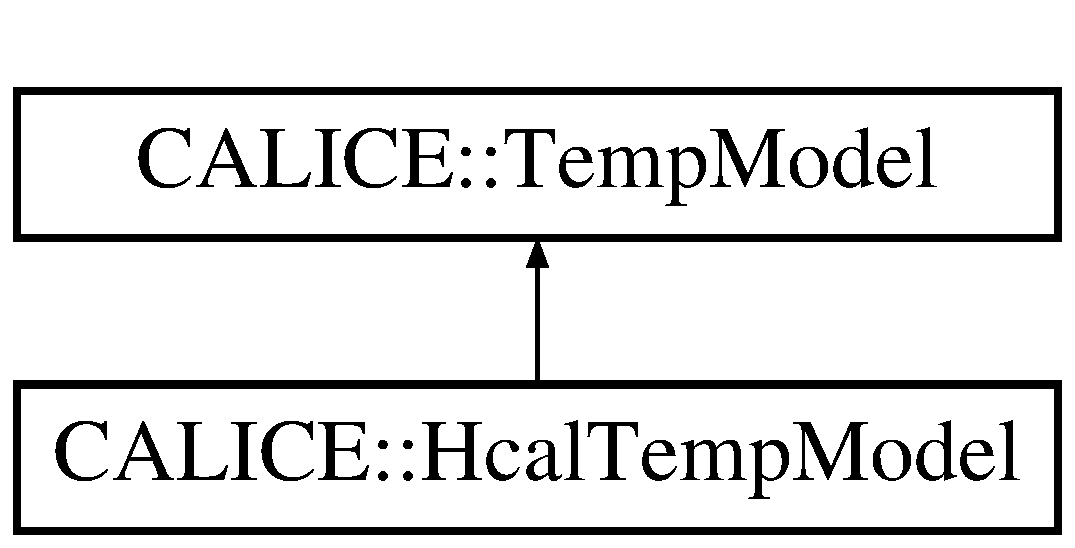
\includegraphics[height=2.000000cm]{classCALICE_1_1HcalTempModel}
\end{center}
\end{figure}
\subsection*{Public Member Functions}
\begin{DoxyCompactItemize}
\item 
virtual float {\bfseries get\-Temp} (lcio\-::\-L\-C\-Collection $\ast$col, unsigned module\-I\-D, unsigned Cell\-Key)\label{classCALICE_1_1HcalTempModel_a76afabe82f217f618a8f20098c9cb91b}

\item 
virtual float {\bfseries get\-Temp\-Error} (lcio\-::\-L\-C\-Collection $\ast$col, unsigned module\-I\-D, unsigned Cell\-Key)\label{classCALICE_1_1HcalTempModel_a4f7355963e4df4c83efb5135a241f785}

\end{DoxyCompactItemize}
\subsection*{Private Attributes}
\begin{DoxyCompactItemize}
\item 
bool {\bfseries \-\_\-first\-Warning}\label{classCALICE_1_1HcalTempModel_a883bb0526e7d1310bedd3f10bfd4e314}

\end{DoxyCompactItemize}


\subsection{Detailed Description}


Definition at line 26 of file Hcal\-Temp\-Model.\-hh.



The documentation for this class was generated from the following file\-:\begin{DoxyCompactItemize}
\item 
Hcal\-Temp\-Model.\-hh\end{DoxyCompactItemize}

\section{histmgr\-:\-:Hist\-Mgr Class Reference}
\label{classhistmgr_1_1HistMgr}\index{histmgr\-::\-Hist\-Mgr@{histmgr\-::\-Hist\-Mgr}}


Manages lists of histograms which can be written to prior assigned files.  




{\ttfamily \#include $<$Hist\-Mgr.\-hh$>$}

\subsection*{Data Structures}
\begin{DoxyCompactItemize}
\item 
class {\bf Group\-\_\-t}
\item 
class {\bf Histogram\-Group\-Data\-\_\-t}
\begin{DoxyCompactList}\small\item\em id, destination file and folder of a histogram group \end{DoxyCompactList}\end{DoxyCompactItemize}
\subsection*{Public Types}
\begin{DoxyCompactItemize}
\item 
enum {\bfseries E\-Collection\-Type} \{ \\*
{\bfseries k\-H1}, 
{\bfseries k\-H2}, 
{\bfseries k\-Profile}, 
{\bfseries k\-Graph}, 
\\*
{\bfseries k\-N\-Types}
 \}
\end{DoxyCompactItemize}
\subsection*{Public Member Functions}
\begin{DoxyCompactItemize}
\item 
bool {\bfseries histogram\-Group\-Exists} (const {\bf Key\-\_\-t} \&group\-\_\-key) const \label{classhistmgr_1_1HistMgr_a4a125aa01302d6ee51520897f5280463}

\item 
{\bf Group\-\_\-t} \& {\bfseries histogram\-Group} (const {\bf Key\-\_\-t} \&group\-\_\-key)\label{classhistmgr_1_1HistMgr_ab07a929a02b75ac6f13c08b36533bd9a}

\item 
const {\bf Group\-\_\-t} \& {\bfseries histogram\-Group} (const {\bf Key\-\_\-t} \&group\-\_\-key) const \label{classhistmgr_1_1HistMgr_a4bb4d3ffbabd7070f791939a684bab6f}

\item 
{\bf Group\-\_\-t} \& {\bf get\-Or\-Createhistogram\-Group} (const {\bf Key\-\_\-t} \&group\-\_\-key)\label{classhistmgr_1_1HistMgr_a3cb22af451aabc860bcee44916d14e04}

\begin{DoxyCompactList}\small\item\em Get the addressed histrogram group. \end{DoxyCompactList}\item 
void {\bf create\-Histogram\-Group} (const {\bf Key\-\_\-t} \&group\-\_\-key)
\begin{DoxyCompactList}\small\item\em Create an empty histogram group to which histograms can be assigned. \end{DoxyCompactList}\item 
lcio\-::\-L\-C\-Collection $\ast$ {\bf create\-Histograms} (const {\bf Key\-\_\-t} \&group\-\_\-key, const {\bf Key\-\_\-t} \&collection\-\_\-key, U\-Int\-\_\-t n\-\_\-hist, const {\bf Hist\-Par} \&par, bool may\-\_\-overwrite=false) noexcept(false)
\begin{DoxyCompactList}\small\item\em create several histograms which will have the same binning and the same name (except of a numeric extension). \end{DoxyCompactList}\item 
lcio\-::\-L\-C\-Collection $\ast$ {\bf create\-Histograms} (const {\bf Key\-\_\-t} \&group\-\_\-key, const {\bf Key\-\_\-t} \&collection\-\_\-key, const E\-V\-E\-N\-T\-::\-String\-Vec \&name\-\_\-list, U\-Int\-\_\-t n\-\_\-hist, const {\bf Hist\-Par} \&par, bool may\-\_\-overwrite=false) noexcept(false)
\begin{DoxyCompactList}\small\item\em create several histograms which will have the same binning and the same name (except of a numeric extension). \end{DoxyCompactList}\item 
lcio\-::\-L\-C\-Collection $\ast$ {\bf create\-Histograms} (const {\bf Key\-\_\-t} \&group\-\_\-key, const {\bf Key\-\_\-t} \&collection\-\_\-key, const lcio\-::\-Int\-Vec \&n\-\_\-hist\-\_\-list, const {\bf Hist\-Par} \&par, bool may\-\_\-overwrite=false) noexcept(false)
\begin{DoxyCompactList}\small\item\em create 2\-D array of histograms which will all have the same binning and the same name (except of a numeric extension). \end{DoxyCompactList}\item 
lcio\-::\-L\-C\-Collection $\ast$ {\bf create\-Histograms} (const {\bf Key\-\_\-t} \&group\-\_\-key, const {\bf Key\-\_\-t} \&collection\-\_\-key, const E\-V\-E\-N\-T\-::\-String\-Vec \&name\-\_\-list, const lcio\-::\-Int\-Vec \&n\-\_\-hist\-\_\-list, const {\bf Hist\-Par} \&par, bool may\-\_\-overwrite=false) noexcept(false)
\begin{DoxyCompactList}\small\item\em create 2\-D array of histograms which will all have the same binning and the same name (except of a numeric extension). \end{DoxyCompactList}\item 
lcio\-::\-L\-C\-Collection $\ast$ {\bf create2\-D\-Histograms} (const {\bf Key\-\_\-t} \&group\-\_\-key, const {\bf Key\-\_\-t} \&collection\-\_\-key, U\-Int\-\_\-t n\-\_\-hist, const {\bf Hist\-Par} \&x\-\_\-par, const {\bf Hist\-Par} \&y\-\_\-par, bool may\-\_\-overwrite=false) noexcept(false)
\begin{DoxyCompactList}\small\item\em create several histograms which will have the same binning and the same name (except of a numeric extension). \end{DoxyCompactList}\item 
lcio\-::\-L\-C\-Collection $\ast$ {\bf create2\-D\-Histograms} (const {\bf Key\-\_\-t} \&group\-\_\-key, const {\bf Key\-\_\-t} \&collection\-\_\-key, const E\-V\-E\-N\-T\-::\-String\-Vec \&name\-\_\-list, U\-Int\-\_\-t n\-\_\-hist, const {\bf Hist\-Par} \&x\-\_\-par, const {\bf Hist\-Par} \&y\-\_\-par, bool may\-\_\-overwrite=false) noexcept(false)
\begin{DoxyCompactList}\small\item\em create several histograms which will have the same binning and the same name (except of a numeric extension). \end{DoxyCompactList}\item 
lcio\-::\-L\-C\-Collection $\ast$ {\bf create2\-D\-Histograms} (const {\bf Key\-\_\-t} \&group\-\_\-key, const {\bf Key\-\_\-t} \&collection\-\_\-key, const lcio\-::\-Int\-Vec \&n\-\_\-hist\-\_\-list, const {\bf Hist\-Par} \&x\-\_\-par, const {\bf Hist\-Par} \&y\-\_\-par, bool may\-\_\-overwrite=false) noexcept(false)
\begin{DoxyCompactList}\small\item\em create 2\-D array of histograms which will all have the same binning and the same name (except of a numeric extension). \end{DoxyCompactList}\item 
lcio\-::\-L\-C\-Collection $\ast$ {\bf create2\-D\-Histograms} (const {\bf Key\-\_\-t} \&group\-\_\-key, const {\bf Key\-\_\-t} \&collection\-\_\-key, const E\-V\-E\-N\-T\-::\-String\-Vec \&name\-\_\-list, const lcio\-::\-Int\-Vec \&n\-\_\-hist\-\_\-list, const {\bf Hist\-Par} \&x\-\_\-par, const {\bf Hist\-Par} \&y\-\_\-par, bool may\-\_\-overwrite=false) noexcept(false)
\begin{DoxyCompactList}\small\item\em create 2\-D array of histograms which will all have the same binning and the same name (except of a numeric extension). \end{DoxyCompactList}\item 
lcio\-::\-L\-C\-Collection $\ast$ {\bf create\-Profile} (const {\bf Key\-\_\-t} \&group\-\_\-key, const {\bf Key\-\_\-t} \&collection\-\_\-key, U\-Int\-\_\-t n\-\_\-hist, const {\bf Hist\-Par} \&par, bool may\-\_\-overwrite=false) noexcept(false)
\begin{DoxyCompactList}\small\item\em create an array of profile histograms which will all have the same binning of the x-\/axis and the same name (except of a numeric extension). \end{DoxyCompactList}\item 
lcio\-::\-L\-C\-Collection $\ast$ {\bf create\-Profile} (const {\bf Key\-\_\-t} \&group\-\_\-key, const {\bf Key\-\_\-t} \&collection\-\_\-key, const E\-V\-E\-N\-T\-::\-String\-Vec \&name\-\_\-list, U\-Int\-\_\-t n\-\_\-hist, const {\bf Hist\-Par} \&par, bool may\-\_\-overwrite=false) noexcept(false)
\begin{DoxyCompactList}\small\item\em create an array of profile histograms which will all have the same binning of the x-\/axis and the same name (except of a numeric extension). \end{DoxyCompactList}\item 
lcio\-::\-L\-C\-Collection $\ast$ {\bf create\-Profile} (const {\bf Key\-\_\-t} \&group\-\_\-key, const {\bf Key\-\_\-t} \&collection\-\_\-key, const lcio\-::\-Int\-Vec \&n\-\_\-hist\-\_\-list, const {\bf Hist\-Par} \&par, bool may\-\_\-overwrite=false) noexcept(false)
\begin{DoxyCompactList}\small\item\em create 2\-D array of profile histograms which will all have the same binning and the same name (except of a numeric extension). \end{DoxyCompactList}\item 
lcio\-::\-L\-C\-Collection $\ast$ {\bf create\-Profile} (const {\bf Key\-\_\-t} \&group\-\_\-key, const {\bf Key\-\_\-t} \&collection\-\_\-key, const E\-V\-E\-N\-T\-::\-String\-Vec \&name\-\_\-list, const lcio\-::\-Int\-Vec \&n\-\_\-hist\-\_\-list, const {\bf Hist\-Par} \&par, bool may\-\_\-overwrite=false) noexcept(false)
\begin{DoxyCompactList}\small\item\em create 2\-D array of profile histograms which will all have the same binning of the x-\/axis. \end{DoxyCompactList}\item 
lcio\-::\-L\-C\-Collection $\ast$ {\bf create\-Graph\-Collection} (const {\bf Key\-\_\-t} \&group\-\_\-key, const {\bf Key\-\_\-t} \&collection\-\_\-key, unsigned int n\-\_\-graphs, const E\-V\-E\-N\-T\-::\-String\-Vec \&type\-\_\-names, unsigned int n\-\_\-expected\-\_\-values, const E\-V\-E\-N\-T\-::\-String\-Vec \&opt\-\_\-major\-\_\-names, bool may\-\_\-overwrite=false) noexcept(false)
\begin{DoxyCompactList}\small\item\em Create a collection of graphs. \end{DoxyCompactList}\item 
lcio\-::\-L\-C\-Collection $\ast$ {\bfseries create\-Graph\-Collection} (const {\bf Key\-\_\-t} \&group\-\_\-key, const {\bf Key\-\_\-t} \&collection\-\_\-key, const std\-::vector$<$ int $>$ \&n\-\_\-graphs, const std\-::vector$<$ std\-::string $>$ \&type\-\_\-names, unsigned int n\-\_\-expected\-\_\-values, const std\-::vector$<$ std\-::string $>$ \&opt\-\_\-major\-\_\-names, bool may\-\_\-overwrite=false) noexcept(false)\label{classhistmgr_1_1HistMgr_a2f05e812013d7bf6c13a2a1a4630b416}

\item 
Double\-\_\-t {\bf get\-N\-Entries\-Total} (const {\bf Key\-\_\-t} \&group\-\_\-key) const 
\begin{DoxyCompactList}\small\item\em return the total number of entries in the whole histogram group. \end{DoxyCompactList}\item 
{\bf Float\-Histogram1\-D} $\ast$ {\bf get\-Histogram} (const {\bf Key\-\_\-t} \&group\-\_\-key, const {\bf Key\-\_\-t} \&hist\-\_\-key, U\-Int\-\_\-t index)
\begin{DoxyCompactList}\small\item\em get a histogram of the collection with the given name. \end{DoxyCompactList}\item 
const {\bf Float\-Histogram1\-D} $\ast$ {\bf get\-Histogram} (const {\bf Key\-\_\-t} \&group\-\_\-key, const {\bf Key\-\_\-t} \&hist\-\_\-key, U\-Int\-\_\-t index) const 
\begin{DoxyCompactList}\small\item\em get a histogram of the collection with the given name (read only). \end{DoxyCompactList}\item 
const {\bf Float\-Histogram1\-D} $\ast$ {\bf get\-Histogram} (const {\bf Key\-\_\-t} \&group\-\_\-key, const {\bf Key\-\_\-t} \&hist\-\_\-key, U\-Int\-\_\-t major\-\_\-index, U\-Int\-\_\-t minor\-\_\-index) const 
\begin{DoxyCompactList}\small\item\em get a histogram of the collection which is organised as a two dimensional array (read only). \end{DoxyCompactList}\item 
{\bf Float\-Histogram1\-D} $\ast$ {\bf get\-Histogram} (const {\bf Key\-\_\-t} \&group\-\_\-key, const {\bf Key\-\_\-t} \&hist\-\_\-key, U\-Int\-\_\-t major\-\_\-index, U\-Int\-\_\-t minor\-\_\-index)
\begin{DoxyCompactList}\small\item\em get a histogram of the collection which is organised as a two dimensional array. \end{DoxyCompactList}\item 
{\bf Float\-Histogram2\-D} $\ast$ {\bf get2\-D\-Histogram} (const {\bf Key\-\_\-t} \&group\-\_\-key, const {\bf Key\-\_\-t} \&hist\-\_\-key, U\-Int\-\_\-t index)
\begin{DoxyCompactList}\small\item\em get a 2\-D histogram of the collection with the given name. \end{DoxyCompactList}\item 
const {\bf Float\-Histogram2\-D} $\ast$ {\bf get2\-D\-Histogram} (const {\bf Key\-\_\-t} \&group\-\_\-key, const {\bf Key\-\_\-t} \&hist\-\_\-key, U\-Int\-\_\-t index) const 
\begin{DoxyCompactList}\small\item\em get a 2\-D histogram of the collection with the given name (read only). \end{DoxyCompactList}\item 
const {\bf Float\-Histogram2\-D} $\ast$ {\bf get2\-D\-Histogram} (const {\bf Key\-\_\-t} \&group\-\_\-key, const {\bf Key\-\_\-t} \&hist\-\_\-key, U\-Int\-\_\-t major\-\_\-index, U\-Int\-\_\-t minor\-\_\-index) const 
\begin{DoxyCompactList}\small\item\em get a 2\-D histogram of the collection which is organised as a two dimensional array (read only). \end{DoxyCompactList}\item 
{\bf Float\-Histogram2\-D} $\ast$ {\bf get2\-D\-Histogram} (const {\bf Key\-\_\-t} \&group\-\_\-key, const {\bf Key\-\_\-t} \&hist\-\_\-key, U\-Int\-\_\-t major\-\_\-index, U\-Int\-\_\-t minor\-\_\-index)
\begin{DoxyCompactList}\small\item\em get a 2\-D histogram of the collection which is organised as a two dimensional array. \end{DoxyCompactList}\item 
bool {\bf exists} (const {\bf Key\-\_\-t} \&group\-\_\-key, const {\bf Key\-\_\-t} \&hist\-\_\-key) const \label{classhistmgr_1_1HistMgr_a8367d06ac7fb422b0b65f44d36e435b8}

\begin{DoxyCompactList}\small\item\em verify if a histogram of the given name exists already. \end{DoxyCompactList}\item 
{\bf Histogram\-Collection\-\_\-t} \& {\bf get\-Histogram\-Collection} (const {\bf Key\-\_\-t} \&group\-\_\-key, const {\bf Key\-\_\-t} \&hist\-\_\-key)\label{classhistmgr_1_1HistMgr_a8589f54841c46f4d807c7d14a944b21b}

\begin{DoxyCompactList}\small\item\em get the one or two dimensional histogram collection. \end{DoxyCompactList}\item 
const {\bf Histogram\-Collection\-\_\-t} \& {\bf get\-Histogram\-Collection} (const {\bf Key\-\_\-t} \&group\-\_\-key, const {\bf Key\-\_\-t} \&hist\-\_\-key) const \label{classhistmgr_1_1HistMgr_a706bda9b86fbfb7ea67645762c4dd16d}

\begin{DoxyCompactList}\small\item\em get the one or two dimensional histogram collection (read only). \end{DoxyCompactList}\item 
{\bf Graph\-Collection\-\_\-t} \& {\bf get\-Graph\-Collection} (const {\bf Key\-\_\-t} \&group\-\_\-key, const {\bf Key\-\_\-t} \&graph\-\_\-key)\label{classhistmgr_1_1HistMgr_a6c5ea89b82f7d9df93423976abdf6470}

\begin{DoxyCompactList}\small\item\em Get a graph collection. \end{DoxyCompactList}\item 
const {\bf Graph\-Collection\-\_\-t} \& {\bf get\-Graph\-Collection} (const {\bf Key\-\_\-t} \&group\-\_\-key, const {\bf Key\-\_\-t} \&graph\-\_\-key) const 
\begin{DoxyCompactList}\small\item\em Get a graph collection. \end{DoxyCompactList}\item 
{\bf Histogram2\-D\-Collection\-\_\-t} \& {\bf get\-Histogram2\-D\-Collection} (const {\bf Key\-\_\-t} \&group\-\_\-key, const {\bf Key\-\_\-t} \&histogram2\-D\-\_\-key)\label{classhistmgr_1_1HistMgr_a3daca1d8debe8c217365403d0fd6e6a4}

\begin{DoxyCompactList}\small\item\em Get a histogram2\-D collection. \end{DoxyCompactList}\item 
const {\bf Histogram2\-D\-Collection\-\_\-t} \& {\bf get\-Histogram2\-D\-Collection} (const {\bf Key\-\_\-t} \&group\-\_\-key, const {\bf Key\-\_\-t} \&histogram2\-D\-\_\-key) const 
\begin{DoxyCompactList}\small\item\em Get a histogram2\-D collection. \end{DoxyCompactList}\item 
{\bf Profile\-Collection\-\_\-t} \& {\bf get\-Profile\-Collection} (const {\bf Key\-\_\-t} \&group\-\_\-key, const {\bf Key\-\_\-t} \&profile\-\_\-key)\label{classhistmgr_1_1HistMgr_a9580175c8b4af1862261acddd6f7b872}

\begin{DoxyCompactList}\small\item\em Get a profile collection. \end{DoxyCompactList}\item 
const {\bf Profile\-Collection\-\_\-t} \& {\bf get\-Profile\-Collection} (const {\bf Key\-\_\-t} \&group\-\_\-key, const {\bf Key\-\_\-t} \&profile\-\_\-key) const 
\begin{DoxyCompactList}\small\item\em Get a profile collection. \end{DoxyCompactList}\item 
void {\bf assign\-File\-Name} (const {\bf Key\-\_\-t} \&group\-\_\-key, const std\-::string \&file\-\_\-name, const std\-::string \&folder\-\_\-name=\char`\"{}\char`\"{})
\begin{DoxyCompactList}\small\item\em get the histogram collection of the given name (read only) The collection must not be deleted. \end{DoxyCompactList}\item 
void {\bf warn\-On\-Unassigned} ()
\begin{DoxyCompactList}\small\item\em Issue a warning for all histogram groups which are not assigned to a file. \end{DoxyCompactList}\item 
void {\bf write\-Histograms} (bool snapshot=false)
\begin{DoxyCompactList}\small\item\em write all histograms groups to the assigned files. \end{DoxyCompactList}\item 
void {\bf write\-Histograms} (const {\bf Key\-\_\-t} \&group\-\_\-key, bool snapshot=false)
\begin{DoxyCompactList}\small\item\em write all histograms of the specified group to the assigned root file. \end{DoxyCompactList}\item 
void {\bf register\-Writer} (const std\-::string \&name, {\bf Hist\-Writer\-Kit} $\ast$kit)
\begin{DoxyCompactList}\small\item\em register a histogram writer. \end{DoxyCompactList}\item 
void {\bfseries list\-Registered\-Groups} () const \label{classhistmgr_1_1HistMgr_a9454383d4576085b061e68e912dc1d09}

\item 
U\-Int\-\_\-t {\bf get\-N\-Groups} () const \label{classhistmgr_1_1HistMgr_a5e6a8a27e9e66d2e0d9e1fd4db24d922}

\begin{DoxyCompactList}\small\item\em Get the number of groups. \end{DoxyCompactList}\item 
void {\bf lock\-Group} (const {\bf Key\-\_\-t} \&group\-\_\-key)
\begin{DoxyCompactList}\small\item\em Lock a histogram group. \end{DoxyCompactList}\item 
void {\bf unlock\-Group} (const {\bf Key\-\_\-t} \&group\-\_\-key)
\begin{DoxyCompactList}\small\item\em Release the lock on the histogram group. \end{DoxyCompactList}\item 
bool {\bf has\-Locked\-Groups} () const \label{classhistmgr_1_1HistMgr_a961080e7358f08fd2f5382038e6952ba}

\begin{DoxyCompactList}\small\item\em Return true if some of the groups are locked. \end{DoxyCompactList}\item 
void {\bf fill\-Group\-List} (std\-::vector$<$ std\-::string $>$ \&dest\-\_\-group\-\_\-list) const 
\begin{DoxyCompactList}\small\item\em Copy the groups names into the given vecotor. \end{DoxyCompactList}\item 
void {\bf fill\-Histogram\-Collection\-List} (const {\bf Key\-\_\-t} \&group\-\_\-key, E\-Collection\-Type type, std\-::vector$<$ std\-::string $>$ \&dest\-\_\-histogram\-\_\-collection\-\_\-list) const 
\begin{DoxyCompactList}\small\item\em Copy the histogram collection names of the specified group to the given vector. \end{DoxyCompactList}\item 
void {\bfseries delete\-Folder} (const std\-::string \&folder)\label{classhistmgr_1_1HistMgr_a1e37c144ebe72c50db57d621ea98c476}

\end{DoxyCompactItemize}
\subsection*{Static Public Member Functions}
\begin{DoxyCompactItemize}
\item 
static E\-Collection\-Type {\bfseries find\-Type} (const std\-::string \&type\-\_\-name)\label{classhistmgr_1_1HistMgr_a182d03588d16279b21ff07c0be7e38fd}

\item 
static std\-::pair$<$ std\-::string, \\*
Hist\-Mgr\-::\-E\-Collection\-Type $>$ {\bf get\-Group\-Name\-And\-Collection\-Type} (const std\-::string \&full\-\_\-name)\label{classhistmgr_1_1HistMgr_abb22cd102ac21320b04232816906e95c}

\begin{DoxyCompactList}\small\item\em Split the name which combines the group name and the collection type into its components. \end{DoxyCompactList}\item 
static {\bf Hist\-Mgr} $\ast$ {\bfseries get\-Instance} ()\label{classhistmgr_1_1HistMgr_ad7376a5e9e63da42eeef529fd6051650}

\item 
static void {\bfseries delete\-Instance} ()\label{classhistmgr_1_1HistMgr_ac08368f8cfb3d0d4afe571076af93b82}

\end{DoxyCompactItemize}
\subsection*{Protected Types}
\begin{DoxyCompactItemize}
\item 
typedef {\bf Key\-Map\-\_\-t}\\*
$<$ {\bf accounting\-\_\-ptr}\\*
$<$ {\bf Histogram2\-D\-Collection\-\_\-t} $>$ $>$ {\bfseries Histogram2\-D\-List\-\_\-t}\label{classhistmgr_1_1HistMgr_a877f8944a0165fd3f95f2c65e39e4136}

\item 
typedef {\bf Key\-Map\-\_\-t}\\*
$<$ {\bf accounting\-\_\-ptr}\\*
$<$ {\bf Histogram\-Collection\-\_\-t} $>$ $>$ {\bfseries Histogram\-List\-\_\-t}\label{classhistmgr_1_1HistMgr_a2204af82055f6ff6c2b2d7e2d8d13c97}

\item 
typedef {\bf Key\-Map\-\_\-t}\\*
$<$ {\bf accounting\-\_\-ptr}\\*
$<$ {\bf Graph\-Collection\-\_\-t} $>$ $>$ {\bfseries Graph\-List\-\_\-t}\label{classhistmgr_1_1HistMgr_a508a8bd989969595b11a6ee8f78b4f5c}

\item 
typedef {\bf Key\-Map\-\_\-t}$<$ {\bf Group\-\_\-t} $>$ {\bfseries Histogram\-Group\-List\-\_\-t}\label{classhistmgr_1_1HistMgr_a3479a617486a4ce270bb116364955885}

\end{DoxyCompactItemize}
\subsection*{Protected Member Functions}
\begin{DoxyCompactItemize}
\item 
{\bf Hist\-Mgr} ()\label{classhistmgr_1_1HistMgr_a8eca0ec734a691b3e5fda89af5c3ab37}

\begin{DoxyCompactList}\small\item\em constructor \end{DoxyCompactList}\item 
{\bf $\sim$\-Hist\-Mgr} ()\label{classhistmgr_1_1HistMgr_a31ee38afe9e57e67e2c1782a850509a1}

\begin{DoxyCompactList}\small\item\em destructor \end{DoxyCompactList}\item 
void {\bfseries write\-Histograms} ({\bf Group\-\_\-t} \&group, const std\-::string \&group\-\_\-name, bool snapshot)\label{classhistmgr_1_1HistMgr_ac79771f2d10dca2e5c4b4a910d130c82}

\end{DoxyCompactItemize}
\subsection*{Protected Attributes}
\begin{DoxyCompactItemize}
\item 
{\bf Histogram\-Group\-List\-\_\-t} {\bfseries \-\_\-histogram\-Group\-List}\label{classhistmgr_1_1HistMgr_a2bc34b78c8b85c0cfebb62805112e93b}

\item 
std\-::map$<$ std\-::string, \\*
{\bf Hist\-Writer\-Kit} $\ast$ $>$ {\bfseries \-\_\-writer\-Kit\-List}\label{classhistmgr_1_1HistMgr_a2b0d5d491ad807e52aaeb1ee0678f6ec}

\item 
{\bf Hist\-Writer\-Kit} $\ast$ {\bfseries \-\_\-writer\-Kit}\label{classhistmgr_1_1HistMgr_a552a6a8461b8d21135a8a8e1a16d05f8}

\end{DoxyCompactItemize}
\subsection*{Static Protected Attributes}
\begin{DoxyCompactItemize}
\item 
static {\bf Hist\-Mgr} $\ast$ {\bfseries \-\_\-\-\_\-hist\-Mgr} =0\label{classhistmgr_1_1HistMgr_a287c31a96bcb8fad1e8b48f88e110510}

\item 
static const char $\ast$ {\bfseries \-\_\-\-\_\-type\-Name} [k\-N\-Types]
\end{DoxyCompactItemize}
\subsection*{Friends}
\begin{DoxyCompactItemize}
\item 
class {\bfseries Hist\-Mgr\-Ptr}\label{classhistmgr_1_1HistMgr_a51e1423cf09cfc432956ca741f8ff236}

\end{DoxyCompactItemize}


\subsection{Detailed Description}
Manages lists of histograms which can be written to prior assigned files. 

Definition at line 43 of file Hist\-Mgr.\-hh.



\subsection{Member Function Documentation}
\index{histmgr\-::\-Hist\-Mgr@{histmgr\-::\-Hist\-Mgr}!assign\-File\-Name@{assign\-File\-Name}}
\index{assign\-File\-Name@{assign\-File\-Name}!histmgr::HistMgr@{histmgr\-::\-Hist\-Mgr}}
\subsubsection[{assign\-File\-Name}]{\setlength{\rightskip}{0pt plus 5cm}void histmgr\-::\-Hist\-Mgr\-::assign\-File\-Name (
\begin{DoxyParamCaption}
\item[{const {\bf Key\-\_\-t} \&}]{group\-\_\-key, }
\item[{const std\-::string \&}]{file\-\_\-name, }
\item[{const std\-::string \&}]{folder\-\_\-name = {\ttfamily \char`\"{}\char`\"{}}}
\end{DoxyParamCaption}
)}\label{classhistmgr_1_1HistMgr_a20e3c96a8ba6175c8036918ca7acb1e2}


get the histogram collection of the given name (read only) The collection must not be deleted. 


\begin{DoxyParams}{Parameters}
{\em name} & of the histogram collection \\
\hline
\end{DoxyParams}
\begin{DoxyReturn}{Returns}
pointer to the histogram collection or zero. get the histogram collection of the given name The collection must not be deleted. 
\end{DoxyReturn}

\begin{DoxyParams}{Parameters}
{\em name} & of the histogram collection \\
\hline
\end{DoxyParams}
\begin{DoxyReturn}{Returns}
pointer to the histogram collection or zero. assign a histogram group to the file of the given name 
\end{DoxyReturn}

\begin{DoxyParams}{Parameters}
{\em group\-\_\-key} & the key of the histogram group \\
\hline
{\em file\-\_\-name} & the name of the file \\
\hline
{\em folder\-\_\-name} & the name of a folder insider the file \\
\hline
\end{DoxyParams}


Definition at line 270 of file Hist\-Mgr.\-cc.



References histmgr\-::\-Hist\-Mgr\-::\-Group\-\_\-t\-::header().



Referenced by histmgr\-::\-Histogram\-Output\-::init().

\index{histmgr\-::\-Hist\-Mgr@{histmgr\-::\-Hist\-Mgr}!create2\-D\-Histograms@{create2\-D\-Histograms}}
\index{create2\-D\-Histograms@{create2\-D\-Histograms}!histmgr::HistMgr@{histmgr\-::\-Hist\-Mgr}}
\subsubsection[{create2\-D\-Histograms}]{\setlength{\rightskip}{0pt plus 5cm}lcio\-::\-L\-C\-Collection$\ast$ histmgr\-::\-Hist\-Mgr\-::create2\-D\-Histograms (
\begin{DoxyParamCaption}
\item[{const {\bf Key\-\_\-t} \&}]{group\-\_\-key, }
\item[{const {\bf Key\-\_\-t} \&}]{collection\-\_\-key, }
\item[{U\-Int\-\_\-t}]{n\-\_\-hist, }
\item[{const {\bf Hist\-Par} \&}]{x\-\_\-par, }
\item[{const {\bf Hist\-Par} \&}]{y\-\_\-par, }
\item[{bool}]{may\-\_\-overwrite = {\ttfamily false}}
\end{DoxyParamCaption}
)\hspace{0.3cm}{\ttfamily [inline]}, {\ttfamily [noexcept]}}\label{classhistmgr_1_1HistMgr_a2ae667341c7eee4db8dcd2fadb1842a4}


create several histograms which will have the same binning and the same name (except of a numeric extension). 

The histograms are only written to a file if the histogram group, to which this histogram belongs, is assigned to a file (\doxyref{histmgr\-::\-Hist\-Mgr\-::assign\-File\-Name}{p.}{classhistmgr_1_1HistMgr_a20e3c96a8ba6175c8036918ca7acb1e2}). 
\begin{DoxyParams}{Parameters}
{\em group\-\_\-key} & the name of the group this histogram belongs to \\
\hline
{\em collection\-\_\-key} & the of the histogram collection \\
\hline
{\em n\-\_\-hist} & the number of histograms to be created \\
\hline
{\em x\-\_\-par} & the binning of the histogram along x \\
\hline
{\em y\-\_\-par} & the binning of the histogram along x \\
\hline
{\em may\-\_\-overwrite} & flag to overwrite or not the histogram, if already existing (default\-: false)\\
\hline
\end{DoxyParams}
\begin{DoxyReturn}{Returns}
the index of the first histogram for 
\end{DoxyReturn}


Definition at line 425 of file Hist\-Mgr.\-hh.



Referenced by create2\-D\-Histograms(), and C\-A\-L\-I\-C\-E\-::\-Square\-Finder\-::init().

\index{histmgr\-::\-Hist\-Mgr@{histmgr\-::\-Hist\-Mgr}!create2\-D\-Histograms@{create2\-D\-Histograms}}
\index{create2\-D\-Histograms@{create2\-D\-Histograms}!histmgr::HistMgr@{histmgr\-::\-Hist\-Mgr}}
\subsubsection[{create2\-D\-Histograms}]{\setlength{\rightskip}{0pt plus 5cm}lcio\-::\-L\-C\-Collection $\ast$ histmgr\-::\-Hist\-Mgr\-::create2\-D\-Histograms (
\begin{DoxyParamCaption}
\item[{const {\bf Key\-\_\-t} \&}]{group\-\_\-key, }
\item[{const {\bf Key\-\_\-t} \&}]{collection\-\_\-key, }
\item[{const E\-V\-E\-N\-T\-::\-String\-Vec \&}]{name\-\_\-list, }
\item[{U\-Int\-\_\-t}]{n\-\_\-hist, }
\item[{const {\bf Hist\-Par} \&}]{x\-\_\-par, }
\item[{const {\bf Hist\-Par} \&}]{y\-\_\-par, }
\item[{bool}]{may\-\_\-overwrite = {\ttfamily false}}
\end{DoxyParamCaption}
)\hspace{0.3cm}{\ttfamily [noexcept]}}\label{classhistmgr_1_1HistMgr_a53b0c5e4ed31409ded872c1ebab1d045}


create several histograms which will have the same binning and the same name (except of a numeric extension). 

The histograms are only written to a file if the histogram group, to which this histogram belongs, is assigned to a file (\doxyref{histmgr\-::\-Hist\-Mgr\-::assign\-File\-Name}{p.}{classhistmgr_1_1HistMgr_a20e3c96a8ba6175c8036918ca7acb1e2}). 
\begin{DoxyParams}{Parameters}
{\em group\-\_\-key} & the name of the group this histogram belongs to \\
\hline
{\em collection\-\_\-key} & the name of the histogram collection \\
\hline
{\em name\-\_\-list} & a vector containing the names of the histograms whose length is either equals n\-\_\-hist or is zero. In the latter case the collection name is used for the all histograms. \\
\hline
{\em n\-\_\-hist} & the number of histograms to be created \\
\hline
{\em x\-\_\-par} & the binning of the x-\/axis of the histogram \\
\hline
{\em y\-\_\-par} & the binning of the y-\/axis of the histogram \\
\hline
{\em may\-\_\-overwrite} & flag to overwrite or not the histogram, if already existing (default\-: false)\\
\hline
\end{DoxyParams}
\begin{DoxyReturn}{Returns}
the index of the first histogram for 
\end{DoxyReturn}


Definition at line 169 of file Hist\-Mgr.\-cc.

\index{histmgr\-::\-Hist\-Mgr@{histmgr\-::\-Hist\-Mgr}!create2\-D\-Histograms@{create2\-D\-Histograms}}
\index{create2\-D\-Histograms@{create2\-D\-Histograms}!histmgr::HistMgr@{histmgr\-::\-Hist\-Mgr}}
\subsubsection[{create2\-D\-Histograms}]{\setlength{\rightskip}{0pt plus 5cm}lcio\-::\-L\-C\-Collection$\ast$ histmgr\-::\-Hist\-Mgr\-::create2\-D\-Histograms (
\begin{DoxyParamCaption}
\item[{const {\bf Key\-\_\-t} \&}]{group\-\_\-key, }
\item[{const {\bf Key\-\_\-t} \&}]{collection\-\_\-key, }
\item[{const lcio\-::\-Int\-Vec \&}]{n\-\_\-hist\-\_\-list, }
\item[{const {\bf Hist\-Par} \&}]{x\-\_\-par, }
\item[{const {\bf Hist\-Par} \&}]{y\-\_\-par, }
\item[{bool}]{may\-\_\-overwrite = {\ttfamily false}}
\end{DoxyParamCaption}
)\hspace{0.3cm}{\ttfamily [inline]}, {\ttfamily [noexcept]}}\label{classhistmgr_1_1HistMgr_ae237911c61f0c89de7f9e499b22c6e11}


create 2\-D array of histograms which will all have the same binning and the same name (except of a numeric extension). 

The histograms are only written to a file if the histogram group, to which this histogram belongs, is assigned to a file (\doxyref{histmgr\-::\-Hist\-Mgr\-::assign\-File\-Name}{p.}{classhistmgr_1_1HistMgr_a20e3c96a8ba6175c8036918ca7acb1e2}). 
\begin{DoxyParams}{Parameters}
{\em group\-\_\-key} & the name of the group this histogram belongs to \\
\hline
{\em collection\-\_\-key} & name of the collection to which the histogram belongs \\
\hline
{\em n\-\_\-hist\-\_\-list} & an array of histograms per major index \\
\hline
{\em x\-\_\-par} & the binning of the x-\/axis of the histogram \\
\hline
{\em y\-\_\-par} & the binning of the y-\/axis the histogram \\
\hline
{\em may\-\_\-overwrite} & flag to overwrite or not the histogram, if existing (default\-: false)\\
\hline
\end{DoxyParams}
\begin{DoxyReturn}{Returns}
the index of the first histogram for 
\end{DoxyReturn}


Definition at line 464 of file Hist\-Mgr.\-hh.



References create2\-D\-Histograms().

\index{histmgr\-::\-Hist\-Mgr@{histmgr\-::\-Hist\-Mgr}!create2\-D\-Histograms@{create2\-D\-Histograms}}
\index{create2\-D\-Histograms@{create2\-D\-Histograms}!histmgr::HistMgr@{histmgr\-::\-Hist\-Mgr}}
\subsubsection[{create2\-D\-Histograms}]{\setlength{\rightskip}{0pt plus 5cm}lcio\-::\-L\-C\-Collection $\ast$ histmgr\-::\-Hist\-Mgr\-::create2\-D\-Histograms (
\begin{DoxyParamCaption}
\item[{const {\bf Key\-\_\-t} \&}]{group\-\_\-key, }
\item[{const {\bf Key\-\_\-t} \&}]{collection\-\_\-key, }
\item[{const E\-V\-E\-N\-T\-::\-String\-Vec \&}]{name\-\_\-list, }
\item[{const lcio\-::\-Int\-Vec \&}]{n\-\_\-hist\-\_\-list, }
\item[{const {\bf Hist\-Par} \&}]{x\-\_\-par, }
\item[{const {\bf Hist\-Par} \&}]{y\-\_\-par, }
\item[{bool}]{may\-\_\-overwrite = {\ttfamily false}}
\end{DoxyParamCaption}
)\hspace{0.3cm}{\ttfamily [noexcept]}}\label{classhistmgr_1_1HistMgr_abcd9a8f2840f1581b5b0c6abe8e4db73}


create 2\-D array of histograms which will all have the same binning and the same name (except of a numeric extension). 

To create an array of 2x3 histograms {\ttfamily  lcio\-::\-Int\-Vec index index.\-push\-\_\-back(3) index.\-push\-\_\-back(3) \doxyref{histmgr\-::\-Key\-\_\-t}{p.}{classhistmgr_1_1Key__t} hist\-\_\-arr\-\_\-2d\-\_\-key(\char`\"{}hist\-\_\-arr\-\_\-2d\char`\"{}) histogram\-List-\/$>$create\-Histograms(group\-\_\-key,hist\-\_\-arr\-\_\-2d\-\_\-key,index,\doxyref{Hist\-Par}{p.}{classHistPar}(4,-\/.\-5,.5)); } The histograms are only written to a file if the histogram group, to which this histogram belongs, is assigned to a file (\doxyref{histmgr\-::\-Hist\-Mgr\-::assign\-File\-Name}{p.}{classhistmgr_1_1HistMgr_a20e3c96a8ba6175c8036918ca7acb1e2}). 
\begin{DoxyParams}{Parameters}
{\em group\-\_\-key} & the name of the group this histogram belongs to \\
\hline
{\em collection\-\_\-key} & name of the collection to which the histogram belongs \\
\hline
{\em name\-\_\-list} & a vector containing the names of the histograms whose length is either one or equals the number of elements of n\-\_\-hist\-\_\-list \\
\hline
{\em n\-\_\-hist\-\_\-list} & an array of histograms per major index \\
\hline
{\em x\-\_\-par} & the binning of the x-\/axis of the histogram \\
\hline
{\em y\-\_\-par} & the binning of the y-\/axis the histogram \\
\hline
{\em may\-\_\-overwrite} & flag to overwrite or not the histogram (default\-: false)\\
\hline
\end{DoxyParams}
\begin{DoxyReturn}{Returns}
the index of the first histogram for 
\end{DoxyReturn}


Definition at line 195 of file Hist\-Mgr.\-cc.

\index{histmgr\-::\-Hist\-Mgr@{histmgr\-::\-Hist\-Mgr}!create\-Graph\-Collection@{create\-Graph\-Collection}}
\index{create\-Graph\-Collection@{create\-Graph\-Collection}!histmgr::HistMgr@{histmgr\-::\-Hist\-Mgr}}
\subsubsection[{create\-Graph\-Collection}]{\setlength{\rightskip}{0pt plus 5cm}lcio\-::\-L\-C\-Collection $\ast$ histmgr\-::\-Hist\-Mgr\-::create\-Graph\-Collection (
\begin{DoxyParamCaption}
\item[{const {\bf Key\-\_\-t} \&}]{group\-\_\-key, }
\item[{const {\bf Key\-\_\-t} \&}]{collection\-\_\-key, }
\item[{unsigned int}]{n\-\_\-graphs, }
\item[{const E\-V\-E\-N\-T\-::\-String\-Vec \&}]{type\-\_\-names, }
\item[{unsigned int}]{n\-\_\-expected\-\_\-values, }
\item[{const E\-V\-E\-N\-T\-::\-String\-Vec \&}]{opt\-\_\-major\-\_\-names, }
\item[{bool}]{may\-\_\-overwrite = {\ttfamily false}}
\end{DoxyParamCaption}
)\hspace{0.3cm}{\ttfamily [noexcept]}}\label{classhistmgr_1_1HistMgr_a89c74c851c7f8cf2b2eef7d358054bd8}


Create a collection of graphs. 

The graphs are addressed by a major and a minor index. The graph collection can for example be used to create mean, rms, min,max graphs per module. The following parameters can be supplied to the collection\-: 
\begin{DoxyItemize}
\item minor\-\_\-width \-: a vector which contains the width for each minor index of the line to be drawn. 
\item minor\-\_\-style \-: a vector which contains the style for each minor index used to draw the line. 
\item minor\-\_\-color \-: a vector which contains the color for each minor index used to draw the line. 
\item major\-\_\-color \-: a vector which contains the color for each major index used to draw the line. This color has precedence over the minor\-\_\-color 
\end{DoxyItemize}

Definition at line 222 of file Hist\-Mgr.\-cc.



Referenced by C\-A\-L\-I\-C\-E\-::\-Average\-History\-Graphs\-::init().

\index{histmgr\-::\-Hist\-Mgr@{histmgr\-::\-Hist\-Mgr}!create\-Histogram\-Group@{create\-Histogram\-Group}}
\index{create\-Histogram\-Group@{create\-Histogram\-Group}!histmgr::HistMgr@{histmgr\-::\-Hist\-Mgr}}
\subsubsection[{create\-Histogram\-Group}]{\setlength{\rightskip}{0pt plus 5cm}void histmgr\-::\-Hist\-Mgr\-::create\-Histogram\-Group (
\begin{DoxyParamCaption}
\item[{const {\bf Key\-\_\-t} \&}]{group\-\_\-key}
\end{DoxyParamCaption}
)\hspace{0.3cm}{\ttfamily [inline]}}\label{classhistmgr_1_1HistMgr_a04aa842cbcd765c10fa47afd05a31b6f}


Create an empty histogram group to which histograms can be assigned. 


\begin{DoxyParams}{Parameters}
{\em group\-\_\-key} & the key to address the group \\
\hline
\end{DoxyParams}
\begin{DoxyReturn}{Returns}
I\-D assigned to the group of the given name The group name is uniqe. If the group exists already the id of the existing group is returned. 
\end{DoxyReturn}
\begin{DoxySeeAlso}{See Also}
\doxyref{create\-Histograms}{p.}{classhistmgr_1_1HistMgr_a777409930c14d08d7aa1c811581d1a34} 
\end{DoxySeeAlso}


Definition at line 313 of file Hist\-Mgr.\-hh.



References get\-Or\-Createhistogram\-Group().



Referenced by C\-A\-L\-I\-C\-E\-::\-Hold\-Scan\-Analysis\-::create\-Histograms(), C\-A\-L\-I\-C\-E\-::\-Pedestal\-Noise\-Histograms\-::init(), C\-A\-L\-I\-C\-E\-::\-Average\-History\-Graphs\-::init(), C\-A\-L\-I\-C\-E\-::\-Trigger\-Analysis\-::init(), and C\-A\-L\-I\-C\-E\-::\-Simple\-Hit\-Search\-::init().

\index{histmgr\-::\-Hist\-Mgr@{histmgr\-::\-Hist\-Mgr}!create\-Histograms@{create\-Histograms}}
\index{create\-Histograms@{create\-Histograms}!histmgr::HistMgr@{histmgr\-::\-Hist\-Mgr}}
\subsubsection[{create\-Histograms}]{\setlength{\rightskip}{0pt plus 5cm}lcio\-::\-L\-C\-Collection$\ast$ histmgr\-::\-Hist\-Mgr\-::create\-Histograms (
\begin{DoxyParamCaption}
\item[{const {\bf Key\-\_\-t} \&}]{group\-\_\-key, }
\item[{const {\bf Key\-\_\-t} \&}]{collection\-\_\-key, }
\item[{U\-Int\-\_\-t}]{n\-\_\-hist, }
\item[{const {\bf Hist\-Par} \&}]{par, }
\item[{bool}]{may\-\_\-overwrite = {\ttfamily false}}
\end{DoxyParamCaption}
)\hspace{0.3cm}{\ttfamily [inline]}, {\ttfamily [noexcept]}}\label{classhistmgr_1_1HistMgr_a777409930c14d08d7aa1c811581d1a34}


create several histograms which will have the same binning and the same name (except of a numeric extension). 

The histograms are only written to a file if the histogram group, to which this histogram belongs, is assigned to a file (\doxyref{histmgr\-::\-Hist\-Mgr\-::assign\-File\-Name}{p.}{classhistmgr_1_1HistMgr_a20e3c96a8ba6175c8036918ca7acb1e2}). 
\begin{DoxyParams}{Parameters}
{\em group\-\_\-key} & the name of the group this histogram belongs to \\
\hline
{\em collection\-\_\-key} & name the of the histogram collection \\
\hline
{\em n\-\_\-hist} & the number of histograms to be created \\
\hline
{\em par} & the binning of the histogram \\
\hline
{\em may\-\_\-overwrite} & flag to overwrite or not the histogram, if already existing (default\-: false)\\
\hline
\end{DoxyParams}
\begin{DoxyReturn}{Returns}
the index of the first histogram for 
\end{DoxyReturn}


Definition at line 341 of file Hist\-Mgr.\-hh.



Referenced by C\-A\-L\-I\-C\-E\-::\-Hold\-Scan\-Analysis\-::create\-Histograms(), create\-Histograms(), C\-A\-L\-I\-C\-E\-::\-Trigger\-Analysis\-::init(), C\-A\-L\-I\-C\-E\-::\-Hold\-Scan\-Analysis\-::init(), C\-A\-L\-I\-C\-E\-::\-Square\-Finder\-::init(), and C\-A\-L\-I\-C\-E\-::\-Clusteriser\-::init().

\index{histmgr\-::\-Hist\-Mgr@{histmgr\-::\-Hist\-Mgr}!create\-Histograms@{create\-Histograms}}
\index{create\-Histograms@{create\-Histograms}!histmgr::HistMgr@{histmgr\-::\-Hist\-Mgr}}
\subsubsection[{create\-Histograms}]{\setlength{\rightskip}{0pt plus 5cm}lcio\-::\-L\-C\-Collection $\ast$ histmgr\-::\-Hist\-Mgr\-::create\-Histograms (
\begin{DoxyParamCaption}
\item[{const {\bf Key\-\_\-t} \&}]{group\-\_\-key, }
\item[{const {\bf Key\-\_\-t} \&}]{collection\-\_\-key, }
\item[{const E\-V\-E\-N\-T\-::\-String\-Vec \&}]{name\-\_\-list, }
\item[{U\-Int\-\_\-t}]{n\-\_\-hist, }
\item[{const {\bf Hist\-Par} \&}]{par, }
\item[{bool}]{may\-\_\-overwrite = {\ttfamily false}}
\end{DoxyParamCaption}
)\hspace{0.3cm}{\ttfamily [noexcept]}}\label{classhistmgr_1_1HistMgr_a93f528b1d0909aa8e93317fd58d99324}


create several histograms which will have the same binning and the same name (except of a numeric extension). 

The histograms are only written to a file if the histogram group, to which this histogram belongs, is assigned to a file (\doxyref{histmgr\-::\-Hist\-Mgr\-::assign\-File\-Name}{p.}{classhistmgr_1_1HistMgr_a20e3c96a8ba6175c8036918ca7acb1e2}). 
\begin{DoxyParams}{Parameters}
{\em group\-\_\-key} & the name of the group this histogram belongs to \\
\hline
{\em collection\-\_\-key} & the name of the histogram collection \\
\hline
{\em name\-\_\-list} & a vector containing the names of the histograms whose length is either equals n\-\_\-hist or is zero. In the latter case the collection name is used for the all histograms. \\
\hline
{\em n\-\_\-hist} & the number of histograms to be created \\
\hline
{\em par} & the binning of the histogram \\
\hline
{\em may\-\_\-overwrite} & flag to overwrite or not the histogram, if already existing (default\-: false)\\
\hline
\end{DoxyParams}
\begin{DoxyReturn}{Returns}
the index of the first histogram for 
\end{DoxyReturn}


Definition at line 117 of file Hist\-Mgr.\-cc.

\index{histmgr\-::\-Hist\-Mgr@{histmgr\-::\-Hist\-Mgr}!create\-Histograms@{create\-Histograms}}
\index{create\-Histograms@{create\-Histograms}!histmgr::HistMgr@{histmgr\-::\-Hist\-Mgr}}
\subsubsection[{create\-Histograms}]{\setlength{\rightskip}{0pt plus 5cm}lcio\-::\-L\-C\-Collection$\ast$ histmgr\-::\-Hist\-Mgr\-::create\-Histograms (
\begin{DoxyParamCaption}
\item[{const {\bf Key\-\_\-t} \&}]{group\-\_\-key, }
\item[{const {\bf Key\-\_\-t} \&}]{collection\-\_\-key, }
\item[{const lcio\-::\-Int\-Vec \&}]{n\-\_\-hist\-\_\-list, }
\item[{const {\bf Hist\-Par} \&}]{par, }
\item[{bool}]{may\-\_\-overwrite = {\ttfamily false}}
\end{DoxyParamCaption}
)\hspace{0.3cm}{\ttfamily [inline]}, {\ttfamily [noexcept]}}\label{classhistmgr_1_1HistMgr_aad621c9ebdadf3ed16bbe0777b05624f}


create 2\-D array of histograms which will all have the same binning and the same name (except of a numeric extension). 

The histograms are only written to a file if the histogram group, to which this histogram belongs, is assigned to a file (\doxyref{histmgr\-::\-Hist\-Mgr\-::assign\-File\-Name}{p.}{classhistmgr_1_1HistMgr_a20e3c96a8ba6175c8036918ca7acb1e2}). 
\begin{DoxyParams}{Parameters}
{\em group\-\_\-key} & the name of the group this histogram belongs to \\
\hline
{\em collection\-\_\-key} & name of the collection to which the histogram belongs \\
\hline
{\em n\-\_\-hist\-\_\-list} & an array of histograms per major index \\
\hline
{\em par} & the binning of the histogram \\
\hline
{\em may\-\_\-overwrite} & flag to overwrite or not the histogram, if already existing (default\-: false)\\
\hline
\end{DoxyParams}
\begin{DoxyReturn}{Returns}
the index of the first histogram for 
\end{DoxyReturn}


Definition at line 378 of file Hist\-Mgr.\-hh.



References create\-Histograms().

\index{histmgr\-::\-Hist\-Mgr@{histmgr\-::\-Hist\-Mgr}!create\-Histograms@{create\-Histograms}}
\index{create\-Histograms@{create\-Histograms}!histmgr::HistMgr@{histmgr\-::\-Hist\-Mgr}}
\subsubsection[{create\-Histograms}]{\setlength{\rightskip}{0pt plus 5cm}lcio\-::\-L\-C\-Collection $\ast$ histmgr\-::\-Hist\-Mgr\-::create\-Histograms (
\begin{DoxyParamCaption}
\item[{const {\bf Key\-\_\-t} \&}]{group\-\_\-key, }
\item[{const {\bf Key\-\_\-t} \&}]{collection\-\_\-key, }
\item[{const E\-V\-E\-N\-T\-::\-String\-Vec \&}]{name\-\_\-list, }
\item[{const lcio\-::\-Int\-Vec \&}]{n\-\_\-hist\-\_\-list, }
\item[{const {\bf Hist\-Par} \&}]{par, }
\item[{bool}]{may\-\_\-overwrite = {\ttfamily false}}
\end{DoxyParamCaption}
)\hspace{0.3cm}{\ttfamily [noexcept]}}\label{classhistmgr_1_1HistMgr_a699fd56d7fcd4e440952aa0e78a37fd7}


create 2\-D array of histograms which will all have the same binning and the same name (except of a numeric extension). 

To create an array of 2x3 histograms {\ttfamily  lcio\-::\-Int\-Vec index index.\-push\-\_\-back(3) index.\-push\-\_\-back(3) \doxyref{histmgr\-::\-Key\-\_\-t}{p.}{classhistmgr_1_1Key__t} hist\-\_\-arr\-\_\-2d\-\_\-key(\char`\"{}hist\-\_\-arr\-\_\-2d\char`\"{}) histogram\-List-\/$>$create\-Histograms(group\-\_\-key,hist\-\_\-arr\-\_\-2d\-\_\-key,index,\doxyref{Hist\-Par}{p.}{classHistPar}(4,-\/.\-5,3.\-5)); } The histograms are only written to a file if the histogram group, to which this histogram belongs, is assigned to a file (\doxyref{histmgr\-::\-Hist\-Mgr\-::assign\-File\-Name}{p.}{classhistmgr_1_1HistMgr_a20e3c96a8ba6175c8036918ca7acb1e2}). 
\begin{DoxyParams}{Parameters}
{\em group\-\_\-key} & the name of the group this histogram belongs to \\
\hline
{\em collection\-\_\-key} & name of the collection to which the histogram belongs \\
\hline
{\em name\-\_\-list} & a vector containing the names of the histograms whose length is either one or equals the number of elements of n\-\_\-hist\-\_\-list \\
\hline
{\em n\-\_\-hist\-\_\-list} & an array of histograms per major index \\
\hline
{\em par} & the binning of the histogram \\
\hline
{\em may\-\_\-overwrite} & flag to overwrite or not the histogram, if already existing (default\-: false)\\
\hline
\end{DoxyParams}
\begin{DoxyReturn}{Returns}
the index of the first histogram for 
\end{DoxyReturn}


Definition at line 142 of file Hist\-Mgr.\-cc.

\index{histmgr\-::\-Hist\-Mgr@{histmgr\-::\-Hist\-Mgr}!create\-Profile@{create\-Profile}}
\index{create\-Profile@{create\-Profile}!histmgr::HistMgr@{histmgr\-::\-Hist\-Mgr}}
\subsubsection[{create\-Profile}]{\setlength{\rightskip}{0pt plus 5cm}lcio\-::\-L\-C\-Collection$\ast$ histmgr\-::\-Hist\-Mgr\-::create\-Profile (
\begin{DoxyParamCaption}
\item[{const {\bf Key\-\_\-t} \&}]{group\-\_\-key, }
\item[{const {\bf Key\-\_\-t} \&}]{collection\-\_\-key, }
\item[{U\-Int\-\_\-t}]{n\-\_\-hist, }
\item[{const {\bf Hist\-Par} \&}]{par, }
\item[{bool}]{may\-\_\-overwrite = {\ttfamily false}}
\end{DoxyParamCaption}
)\hspace{0.3cm}{\ttfamily [inline]}, {\ttfamily [noexcept]}}\label{classhistmgr_1_1HistMgr_a2b7fb559c67fee959812717585e1ebd2}


create an array of profile histograms which will all have the same binning of the x-\/axis and the same name (except of a numeric extension). 


\begin{DoxyParams}{Parameters}
{\em group\-\_\-key} & the name of the group this profile histogram belongs to \\
\hline
{\em collection\-\_\-key} & name of the collection to which the histogram belongs \\
\hline
{\em n\-\_\-hist} & the number of histograms to be created \\
\hline
{\em par} & the binning of the x-\/axis of the profile histogram \\
\hline
{\em may\-\_\-overwrite} & flag to overwrite or not the histogram, if already existing (default\-: false)\\
\hline
\end{DoxyParams}
\begin{DoxyReturn}{Returns}
a pointer to the the profile histogram collection 
\end{DoxyReturn}


Definition at line 511 of file Hist\-Mgr.\-hh.



Referenced by create\-Profile().

\index{histmgr\-::\-Hist\-Mgr@{histmgr\-::\-Hist\-Mgr}!create\-Profile@{create\-Profile}}
\index{create\-Profile@{create\-Profile}!histmgr::HistMgr@{histmgr\-::\-Hist\-Mgr}}
\subsubsection[{create\-Profile}]{\setlength{\rightskip}{0pt plus 5cm}lcio\-::\-L\-C\-Collection$\ast$ histmgr\-::\-Hist\-Mgr\-::create\-Profile (
\begin{DoxyParamCaption}
\item[{const {\bf Key\-\_\-t} \&}]{group\-\_\-key, }
\item[{const {\bf Key\-\_\-t} \&}]{collection\-\_\-key, }
\item[{const E\-V\-E\-N\-T\-::\-String\-Vec \&}]{name\-\_\-list, }
\item[{U\-Int\-\_\-t}]{n\-\_\-hist, }
\item[{const {\bf Hist\-Par} \&}]{par, }
\item[{bool}]{may\-\_\-overwrite = {\ttfamily false}}
\end{DoxyParamCaption}
)\hspace{0.3cm}{\ttfamily [noexcept]}}\label{classhistmgr_1_1HistMgr_ab5396f26178d419d4e89e617fcaf0d1c}


create an array of profile histograms which will all have the same binning of the x-\/axis and the same name (except of a numeric extension). 


\begin{DoxyParams}{Parameters}
{\em group\-\_\-key} & the name of the group this profile histogram belongs to \\
\hline
{\em collection\-\_\-key} & name of the collection to which the histogram belongs \\
\hline
{\em name\-\_\-list} & a vector containing the names of the profile histograms whose length is either one or equals the number of elements of n\-\_\-hist\-\_\-list \\
\hline
{\em n\-\_\-hist} & the number of histograms to be created \\
\hline
{\em par} & the binning of the x-\/axis of the profile histogram \\
\hline
{\em may\-\_\-overwrite} & flag to overwrite or not the histogram, if already existing (default\-: false)\\
\hline
\end{DoxyParams}
\begin{DoxyReturn}{Returns}
a pointer to the the profile histogram collection 
\end{DoxyReturn}
\index{histmgr\-::\-Hist\-Mgr@{histmgr\-::\-Hist\-Mgr}!create\-Profile@{create\-Profile}}
\index{create\-Profile@{create\-Profile}!histmgr::HistMgr@{histmgr\-::\-Hist\-Mgr}}
\subsubsection[{create\-Profile}]{\setlength{\rightskip}{0pt plus 5cm}lcio\-::\-L\-C\-Collection$\ast$ histmgr\-::\-Hist\-Mgr\-::create\-Profile (
\begin{DoxyParamCaption}
\item[{const {\bf Key\-\_\-t} \&}]{group\-\_\-key, }
\item[{const {\bf Key\-\_\-t} \&}]{collection\-\_\-key, }
\item[{const lcio\-::\-Int\-Vec \&}]{n\-\_\-hist\-\_\-list, }
\item[{const {\bf Hist\-Par} \&}]{par, }
\item[{bool}]{may\-\_\-overwrite = {\ttfamily false}}
\end{DoxyParamCaption}
)\hspace{0.3cm}{\ttfamily [inline]}, {\ttfamily [noexcept]}}\label{classhistmgr_1_1HistMgr_ad1c738fcfbd7514d438ce13e2f005029}


create 2\-D array of profile histograms which will all have the same binning and the same name (except of a numeric extension). 


\begin{DoxyParams}{Parameters}
{\em group\-\_\-key} & the name of the group this profile histogram belongs to \\
\hline
{\em collection\-\_\-key} & name of the collection to which the histogram belongs \\
\hline
{\em n\-\_\-hist\-\_\-list} & an array of histograms per major index \\
\hline
{\em par} & the binning of the x-\/axis of the profile histogram \\
\hline
{\em may\-\_\-overwrite} & flag to overwrite or not the histogram, if already existing (default\-: false)\\
\hline
\end{DoxyParams}
\begin{DoxyReturn}{Returns}
a pointer to the the profile histogram collection 
\end{DoxyReturn}


Definition at line 544 of file Hist\-Mgr.\-hh.



References create\-Profile().

\index{histmgr\-::\-Hist\-Mgr@{histmgr\-::\-Hist\-Mgr}!create\-Profile@{create\-Profile}}
\index{create\-Profile@{create\-Profile}!histmgr::HistMgr@{histmgr\-::\-Hist\-Mgr}}
\subsubsection[{create\-Profile}]{\setlength{\rightskip}{0pt plus 5cm}lcio\-::\-L\-C\-Collection$\ast$ histmgr\-::\-Hist\-Mgr\-::create\-Profile (
\begin{DoxyParamCaption}
\item[{const {\bf Key\-\_\-t} \&}]{group\-\_\-key, }
\item[{const {\bf Key\-\_\-t} \&}]{collection\-\_\-key, }
\item[{const E\-V\-E\-N\-T\-::\-String\-Vec \&}]{name\-\_\-list, }
\item[{const lcio\-::\-Int\-Vec \&}]{n\-\_\-hist\-\_\-list, }
\item[{const {\bf Hist\-Par} \&}]{par, }
\item[{bool}]{may\-\_\-overwrite = {\ttfamily false}}
\end{DoxyParamCaption}
)\hspace{0.3cm}{\ttfamily [noexcept]}}\label{classhistmgr_1_1HistMgr_a4770d6326280cddda496ded64ac1d2bb}


create 2\-D array of profile histograms which will all have the same binning of the x-\/axis. 


\begin{DoxyParams}{Parameters}
{\em group\-\_\-key} & the name of the group this profile histogram belongs to \\
\hline
{\em collection\-\_\-key} & name of the collection to which the histogram belongs \\
\hline
{\em name\-\_\-list} & a vector containing the names of the profile histograms whose length is either one or equals the number of elements of n\-\_\-hist\-\_\-list \\
\hline
{\em n\-\_\-hist\-\_\-list} & an array of histograms per major index \\
\hline
{\em par} & the binning of the x-\/axis of the profile histogram \\
\hline
{\em may\-\_\-overwrite} & flag to overwrite or not the histogram, if already existing (default\-: false)\\
\hline
\end{DoxyParams}
\begin{DoxyReturn}{Returns}
a pointer to the the profile histogram collection 
\end{DoxyReturn}
\index{histmgr\-::\-Hist\-Mgr@{histmgr\-::\-Hist\-Mgr}!fill\-Group\-List@{fill\-Group\-List}}
\index{fill\-Group\-List@{fill\-Group\-List}!histmgr::HistMgr@{histmgr\-::\-Hist\-Mgr}}
\subsubsection[{fill\-Group\-List}]{\setlength{\rightskip}{0pt plus 5cm}void histmgr\-::\-Hist\-Mgr\-::fill\-Group\-List (
\begin{DoxyParamCaption}
\item[{std\-::vector$<$ std\-::string $>$ \&}]{dest\-\_\-group\-\_\-list}
\end{DoxyParamCaption}
) const}\label{classhistmgr_1_1HistMgr_afe03f9a977b33e3d369a9c4133b74716}


Copy the groups names into the given vecotor. 


\begin{DoxyParams}{Parameters}
{\em dest\-\_\-group\-\_\-list} & the vector which will be filled with the group names. First the given vector will be cleared. Then all group names will be copied to it. \\
\hline
\end{DoxyParams}


Definition at line 317 of file Hist\-Mgr.\-cc.

\index{histmgr\-::\-Hist\-Mgr@{histmgr\-::\-Hist\-Mgr}!fill\-Histogram\-Collection\-List@{fill\-Histogram\-Collection\-List}}
\index{fill\-Histogram\-Collection\-List@{fill\-Histogram\-Collection\-List}!histmgr::HistMgr@{histmgr\-::\-Hist\-Mgr}}
\subsubsection[{fill\-Histogram\-Collection\-List}]{\setlength{\rightskip}{0pt plus 5cm}void histmgr\-::\-Hist\-Mgr\-::fill\-Histogram\-Collection\-List (
\begin{DoxyParamCaption}
\item[{const {\bf Key\-\_\-t} \&}]{group\-\_\-key, }
\item[{E\-Collection\-Type}]{type, }
\item[{std\-::vector$<$ std\-::string $>$ \&}]{dest\-\_\-histogram\-\_\-collection\-\_\-list}
\end{DoxyParamCaption}
) const}\label{classhistmgr_1_1HistMgr_aae8c3abe639e31993241569127fbff3e}


Copy the histogram collection names of the specified group to the given vector. 


\begin{DoxyParams}{Parameters}
{\em group\-\_\-key} & the name of the group whose histogram collection are considered. \\
\hline
{\em type} & type of the collection to which the histogram belongs \\
\hline
{\em dest\-\_\-histogram\-\_\-collection\-\_\-list} & the vector which will be filled with the names of the histgram collections which are associated to the specified group. First the given vector will be cleared. Then all the names of the histogram collections which are associated to the specfied group will be copied to it. \\
\hline
\end{DoxyParams}


Definition at line 354 of file Hist\-Mgr.\-cc.



References histmgr\-::\-Hist\-Mgr\-::\-Group\-\_\-t\-::graph\-Collection(), histmgr\-::\-Hist\-Mgr\-::\-Group\-\_\-t\-::histogram2\-D\-Collection(), histmgr\-::\-Hist\-Mgr\-::\-Group\-\_\-t\-::histogram\-Collection(), histmgr\-::\-Graph\-Collection\-\_\-t\-::n(), histmgr\-::\-Profile\-Collection\-\_\-t\-::n(), histmgr\-::\-Histogram\-Collection\-\_\-t\-::n(), histmgr\-::\-Histogram2\-D\-Collection\-\_\-t\-::n(), histmgr\-::\-Hist\-Mgr\-::\-Group\-\_\-t\-::name\-List\-Iterators(), and histmgr\-::\-Hist\-Mgr\-::\-Group\-\_\-t\-::profile\-Collection().

\index{histmgr\-::\-Hist\-Mgr@{histmgr\-::\-Hist\-Mgr}!get2\-D\-Histogram@{get2\-D\-Histogram}}
\index{get2\-D\-Histogram@{get2\-D\-Histogram}!histmgr::HistMgr@{histmgr\-::\-Hist\-Mgr}}
\subsubsection[{get2\-D\-Histogram}]{\setlength{\rightskip}{0pt plus 5cm}{\bf Float\-Histogram2\-D}$\ast$ histmgr\-::\-Hist\-Mgr\-::get2\-D\-Histogram (
\begin{DoxyParamCaption}
\item[{const {\bf Key\-\_\-t} \&}]{group\-\_\-key, }
\item[{const {\bf Key\-\_\-t} \&}]{hist\-\_\-key, }
\item[{U\-Int\-\_\-t}]{index}
\end{DoxyParamCaption}
)\hspace{0.3cm}{\ttfamily [inline]}}\label{classhistmgr_1_1HistMgr_ab4da74dcb5d34f186073d4a1fda4e831}


get a 2\-D histogram of the collection with the given name. 

The histogram must not be deleted. Generally, the method does not check the validity of the index. the method throws exceptions if the collection does not exist or If B\-O\-U\-N\-D\-A\-R\-Y\-\_\-\-C\-H\-E\-C\-K is defined and the index is out of range.


\begin{DoxyParams}{Parameters}
{\em group\-\_\-key} & name of the histogram's group \\
\hline
{\em hist\-\_\-key} & name of the histogram \\
\hline
{\em index} & the index within the collection \\
\hline
\end{DoxyParams}
\begin{DoxyReturn}{Returns}
pointer to the histogram collection or zero. 
\end{DoxyReturn}


Definition at line 718 of file Hist\-Mgr.\-hh.

\index{histmgr\-::\-Hist\-Mgr@{histmgr\-::\-Hist\-Mgr}!get2\-D\-Histogram@{get2\-D\-Histogram}}
\index{get2\-D\-Histogram@{get2\-D\-Histogram}!histmgr::HistMgr@{histmgr\-::\-Hist\-Mgr}}
\subsubsection[{get2\-D\-Histogram}]{\setlength{\rightskip}{0pt plus 5cm}const {\bf Float\-Histogram2\-D}$\ast$ histmgr\-::\-Hist\-Mgr\-::get2\-D\-Histogram (
\begin{DoxyParamCaption}
\item[{const {\bf Key\-\_\-t} \&}]{group\-\_\-key, }
\item[{const {\bf Key\-\_\-t} \&}]{hist\-\_\-key, }
\item[{U\-Int\-\_\-t}]{index}
\end{DoxyParamCaption}
) const\hspace{0.3cm}{\ttfamily [inline]}}\label{classhistmgr_1_1HistMgr_a7f3d08a4bcde4bc739ca9fc1642e8120}


get a 2\-D histogram of the collection with the given name (read only). 

The histogram must not be deleted. Generally, the method does not check the validity of the index. the method throws exceptions if the collection does not exist or If B\-O\-U\-N\-D\-A\-R\-Y\-\_\-\-C\-H\-E\-C\-K is defined and the index is out of range.


\begin{DoxyParams}{Parameters}
{\em group\-\_\-key} & name of the histogram's group \\
\hline
{\em hist\-\_\-key} & name of the histogram \\
\hline
{\em index} & the index within the collection \\
\hline
\end{DoxyParams}
\begin{DoxyReturn}{Returns}
pointer to the histogram collection or zero. 
\end{DoxyReturn}


Definition at line 744 of file Hist\-Mgr.\-hh.

\index{histmgr\-::\-Hist\-Mgr@{histmgr\-::\-Hist\-Mgr}!get2\-D\-Histogram@{get2\-D\-Histogram}}
\index{get2\-D\-Histogram@{get2\-D\-Histogram}!histmgr::HistMgr@{histmgr\-::\-Hist\-Mgr}}
\subsubsection[{get2\-D\-Histogram}]{\setlength{\rightskip}{0pt plus 5cm}const {\bf Float\-Histogram2\-D}$\ast$ histmgr\-::\-Hist\-Mgr\-::get2\-D\-Histogram (
\begin{DoxyParamCaption}
\item[{const {\bf Key\-\_\-t} \&}]{group\-\_\-key, }
\item[{const {\bf Key\-\_\-t} \&}]{hist\-\_\-key, }
\item[{U\-Int\-\_\-t}]{major\-\_\-index, }
\item[{U\-Int\-\_\-t}]{minor\-\_\-index}
\end{DoxyParamCaption}
) const\hspace{0.3cm}{\ttfamily [inline]}}\label{classhistmgr_1_1HistMgr_a8cf0e7bc525eae6507dbc15805eed94c}


get a 2\-D histogram of the collection which is organised as a two dimensional array (read only). 

The histogram must not be deleted. Generally, the method does not check the validity of the indices. the method throws exceptions if the collection does not exist or If B\-O\-U\-N\-D\-A\-R\-Y\-\_\-\-C\-H\-E\-C\-K is defined and the indices are out of range.


\begin{DoxyParams}{Parameters}
{\em group\-\_\-key} & name of the histogram's group \\
\hline
{\em hist\-\_\-key} & name of the histogram \\
\hline
{\em major\-\_\-index} & the major index within the collection \\
\hline
{\em minor\-\_\-index} & the major index within the collection \\
\hline
\end{DoxyParams}
\begin{DoxyReturn}{Returns}
pointer to the histogram collection or zero. 
\end{DoxyReturn}


Definition at line 770 of file Hist\-Mgr.\-hh.

\index{histmgr\-::\-Hist\-Mgr@{histmgr\-::\-Hist\-Mgr}!get2\-D\-Histogram@{get2\-D\-Histogram}}
\index{get2\-D\-Histogram@{get2\-D\-Histogram}!histmgr::HistMgr@{histmgr\-::\-Hist\-Mgr}}
\subsubsection[{get2\-D\-Histogram}]{\setlength{\rightskip}{0pt plus 5cm}{\bf Float\-Histogram2\-D}$\ast$ histmgr\-::\-Hist\-Mgr\-::get2\-D\-Histogram (
\begin{DoxyParamCaption}
\item[{const {\bf Key\-\_\-t} \&}]{group\-\_\-key, }
\item[{const {\bf Key\-\_\-t} \&}]{hist\-\_\-key, }
\item[{U\-Int\-\_\-t}]{major\-\_\-index, }
\item[{U\-Int\-\_\-t}]{minor\-\_\-index}
\end{DoxyParamCaption}
)\hspace{0.3cm}{\ttfamily [inline]}}\label{classhistmgr_1_1HistMgr_a8efc6e2c08e1a92d5a37690b04904cd3}


get a 2\-D histogram of the collection which is organised as a two dimensional array. 

The histogram must not be deleted. Generally, the method does not check the validity of the indices. the method throws exceptions if the collection does not exist or If B\-O\-U\-N\-D\-A\-R\-Y\-\_\-\-C\-H\-E\-C\-K is defined and the indices are out of range.


\begin{DoxyParams}{Parameters}
{\em group\-\_\-key} & name of the histogram's group \\
\hline
{\em hist\-\_\-key} & name of the histogram \\
\hline
{\em major\-\_\-index} & the major index within the collection \\
\hline
{\em minor\-\_\-index} & the major index within the collection \\
\hline
\end{DoxyParams}
\begin{DoxyReturn}{Returns}
pointer to the histogram collection or zero. 
\end{DoxyReturn}


Definition at line 797 of file Hist\-Mgr.\-hh.

\index{histmgr\-::\-Hist\-Mgr@{histmgr\-::\-Hist\-Mgr}!get\-Graph\-Collection@{get\-Graph\-Collection}}
\index{get\-Graph\-Collection@{get\-Graph\-Collection}!histmgr::HistMgr@{histmgr\-::\-Hist\-Mgr}}
\subsubsection[{get\-Graph\-Collection}]{\setlength{\rightskip}{0pt plus 5cm}const {\bf Graph\-Collection\-\_\-t}\& histmgr\-::\-Hist\-Mgr\-::get\-Graph\-Collection (
\begin{DoxyParamCaption}
\item[{const {\bf Key\-\_\-t} \&}]{group\-\_\-key, }
\item[{const {\bf Key\-\_\-t} \&}]{graph\-\_\-key}
\end{DoxyParamCaption}
) const\hspace{0.3cm}{\ttfamily [inline]}}\label{classhistmgr_1_1HistMgr_adceab95da3bf897045779682cbfff2d9}


Get a graph collection. 

(read only). 

Definition at line 865 of file Hist\-Mgr.\-hh.

\index{histmgr\-::\-Hist\-Mgr@{histmgr\-::\-Hist\-Mgr}!get\-Histogram@{get\-Histogram}}
\index{get\-Histogram@{get\-Histogram}!histmgr::HistMgr@{histmgr\-::\-Hist\-Mgr}}
\subsubsection[{get\-Histogram}]{\setlength{\rightskip}{0pt plus 5cm}{\bf Float\-Histogram1\-D}$\ast$ histmgr\-::\-Hist\-Mgr\-::get\-Histogram (
\begin{DoxyParamCaption}
\item[{const {\bf Key\-\_\-t} \&}]{group\-\_\-key, }
\item[{const {\bf Key\-\_\-t} \&}]{hist\-\_\-key, }
\item[{U\-Int\-\_\-t}]{index}
\end{DoxyParamCaption}
)\hspace{0.3cm}{\ttfamily [inline]}}\label{classhistmgr_1_1HistMgr_a797aae0e8ced26bca02e41ed4b83c72b}


get a histogram of the collection with the given name. 

The histogram must not be deleted. Generally, the method does not check the validity of the index. the method throws exceptions if the collection does not exist or If B\-O\-U\-N\-D\-A\-R\-Y\-\_\-\-C\-H\-E\-C\-K is defined and the index is out of range.


\begin{DoxyParams}{Parameters}
{\em group\-\_\-key} & name of the histogram's group \\
\hline
{\em hist\-\_\-key} & name of the histogram \\
\hline
{\em index} & the index within the collection \\
\hline
\end{DoxyParams}
\begin{DoxyReturn}{Returns}
pointer to the histogram collection or zero. 
\end{DoxyReturn}


Definition at line 614 of file Hist\-Mgr.\-hh.

\index{histmgr\-::\-Hist\-Mgr@{histmgr\-::\-Hist\-Mgr}!get\-Histogram@{get\-Histogram}}
\index{get\-Histogram@{get\-Histogram}!histmgr::HistMgr@{histmgr\-::\-Hist\-Mgr}}
\subsubsection[{get\-Histogram}]{\setlength{\rightskip}{0pt plus 5cm}const {\bf Float\-Histogram1\-D}$\ast$ histmgr\-::\-Hist\-Mgr\-::get\-Histogram (
\begin{DoxyParamCaption}
\item[{const {\bf Key\-\_\-t} \&}]{group\-\_\-key, }
\item[{const {\bf Key\-\_\-t} \&}]{hist\-\_\-key, }
\item[{U\-Int\-\_\-t}]{index}
\end{DoxyParamCaption}
) const\hspace{0.3cm}{\ttfamily [inline]}}\label{classhistmgr_1_1HistMgr_ab85919d0fb60f4c9d3916a89822ffbfe}


get a histogram of the collection with the given name (read only). 

The histogram must not be deleted. Generally, the method does not check the validity of the index. the method throws exceptions if the collection does not exist or If B\-O\-U\-N\-D\-A\-R\-Y\-\_\-\-C\-H\-E\-C\-K is defined and the index is out of range.


\begin{DoxyParams}{Parameters}
{\em group\-\_\-key} & name of the histogram's group \\
\hline
{\em hist\-\_\-key} & name of the histogram \\
\hline
{\em index} & the index within the collection \\
\hline
\end{DoxyParams}
\begin{DoxyReturn}{Returns}
pointer to the histogram collection or zero. 
\end{DoxyReturn}


Definition at line 640 of file Hist\-Mgr.\-hh.

\index{histmgr\-::\-Hist\-Mgr@{histmgr\-::\-Hist\-Mgr}!get\-Histogram@{get\-Histogram}}
\index{get\-Histogram@{get\-Histogram}!histmgr::HistMgr@{histmgr\-::\-Hist\-Mgr}}
\subsubsection[{get\-Histogram}]{\setlength{\rightskip}{0pt plus 5cm}const {\bf Float\-Histogram1\-D}$\ast$ histmgr\-::\-Hist\-Mgr\-::get\-Histogram (
\begin{DoxyParamCaption}
\item[{const {\bf Key\-\_\-t} \&}]{group\-\_\-key, }
\item[{const {\bf Key\-\_\-t} \&}]{hist\-\_\-key, }
\item[{U\-Int\-\_\-t}]{major\-\_\-index, }
\item[{U\-Int\-\_\-t}]{minor\-\_\-index}
\end{DoxyParamCaption}
) const\hspace{0.3cm}{\ttfamily [inline]}}\label{classhistmgr_1_1HistMgr_a488e892b3b341d86992f3e52ddc2dfc6}


get a histogram of the collection which is organised as a two dimensional array (read only). 

The histogram must not be deleted. Generally, the method does not check the validity of the indices. the method throws exceptions if the collection does not exist or If B\-O\-U\-N\-D\-A\-R\-Y\-\_\-\-C\-H\-E\-C\-K is defined and the indices are out of range.


\begin{DoxyParams}{Parameters}
{\em group\-\_\-key} & name of the histogram's group \\
\hline
{\em hist\-\_\-key} & name of the histogram \\
\hline
{\em major\-\_\-index} & the major index within the collection \\
\hline
{\em minor\-\_\-index} & the major index within the collection \\
\hline
\end{DoxyParams}
\begin{DoxyReturn}{Returns}
pointer to the histogram collection or zero. 
\end{DoxyReturn}


Definition at line 666 of file Hist\-Mgr.\-hh.

\index{histmgr\-::\-Hist\-Mgr@{histmgr\-::\-Hist\-Mgr}!get\-Histogram@{get\-Histogram}}
\index{get\-Histogram@{get\-Histogram}!histmgr::HistMgr@{histmgr\-::\-Hist\-Mgr}}
\subsubsection[{get\-Histogram}]{\setlength{\rightskip}{0pt plus 5cm}{\bf Float\-Histogram1\-D}$\ast$ histmgr\-::\-Hist\-Mgr\-::get\-Histogram (
\begin{DoxyParamCaption}
\item[{const {\bf Key\-\_\-t} \&}]{group\-\_\-key, }
\item[{const {\bf Key\-\_\-t} \&}]{hist\-\_\-key, }
\item[{U\-Int\-\_\-t}]{major\-\_\-index, }
\item[{U\-Int\-\_\-t}]{minor\-\_\-index}
\end{DoxyParamCaption}
)\hspace{0.3cm}{\ttfamily [inline]}}\label{classhistmgr_1_1HistMgr_a88b3f269d21c0bfd28671ca1bca8d47b}


get a histogram of the collection which is organised as a two dimensional array. 

The histogram must not be deleted. Generally, the method does not check the validity of the indices. the method throws exceptions if the collection does not exist or If B\-O\-U\-N\-D\-A\-R\-Y\-\_\-\-C\-H\-E\-C\-K is defined and the indices are out of range.


\begin{DoxyParams}{Parameters}
{\em group\-\_\-key} & name of the histogram's group \\
\hline
{\em hist\-\_\-key} & name of the histogram \\
\hline
{\em major\-\_\-index} & the major index within the collection \\
\hline
{\em minor\-\_\-index} & the major index within the collection \\
\hline
\end{DoxyParams}
\begin{DoxyReturn}{Returns}
pointer to the histogram collection or zero. 
\end{DoxyReturn}


Definition at line 693 of file Hist\-Mgr.\-hh.

\index{histmgr\-::\-Hist\-Mgr@{histmgr\-::\-Hist\-Mgr}!get\-Histogram2\-D\-Collection@{get\-Histogram2\-D\-Collection}}
\index{get\-Histogram2\-D\-Collection@{get\-Histogram2\-D\-Collection}!histmgr::HistMgr@{histmgr\-::\-Hist\-Mgr}}
\subsubsection[{get\-Histogram2\-D\-Collection}]{\setlength{\rightskip}{0pt plus 5cm}const {\bf Histogram2\-D\-Collection\-\_\-t}\& histmgr\-::\-Hist\-Mgr\-::get\-Histogram2\-D\-Collection (
\begin{DoxyParamCaption}
\item[{const {\bf Key\-\_\-t} \&}]{group\-\_\-key, }
\item[{const {\bf Key\-\_\-t} \&}]{histogram2\-D\-\_\-key}
\end{DoxyParamCaption}
) const\hspace{0.3cm}{\ttfamily [inline]}}\label{classhistmgr_1_1HistMgr_a23378a9d9865d311a9dbfd163a66042c}


Get a histogram2\-D collection. 

(read only). 

Definition at line 883 of file Hist\-Mgr.\-hh.

\index{histmgr\-::\-Hist\-Mgr@{histmgr\-::\-Hist\-Mgr}!get\-N\-Entries\-Total@{get\-N\-Entries\-Total}}
\index{get\-N\-Entries\-Total@{get\-N\-Entries\-Total}!histmgr::HistMgr@{histmgr\-::\-Hist\-Mgr}}
\subsubsection[{get\-N\-Entries\-Total}]{\setlength{\rightskip}{0pt plus 5cm}Double\-\_\-t histmgr\-::\-Hist\-Mgr\-::get\-N\-Entries\-Total (
\begin{DoxyParamCaption}
\item[{const {\bf Key\-\_\-t} \&}]{group\-\_\-key}
\end{DoxyParamCaption}
) const}\label{classhistmgr_1_1HistMgr_a82abb61111cc4eda9f15a3d3a36a1114}


return the total number of entries in the whole histogram group. 



Definition at line 409 of file Hist\-Mgr.\-cc.



References histmgr\-::\-Histogram1\-D\-::entries(), histmgr\-::\-Histogram\-Collection\-\_\-t\-::histogram(), histmgr\-::\-Histogram\-Collection\-\_\-t\-::is2\-D(), histmgr\-::\-Histogram\-Collection\-\_\-t\-::n(), histmgr\-::\-Histogram\-Collection\-\_\-t\-::n\-Major(), and histmgr\-::\-Histogram\-Collection\-\_\-t\-::n\-Minor().

\index{histmgr\-::\-Hist\-Mgr@{histmgr\-::\-Hist\-Mgr}!get\-Profile\-Collection@{get\-Profile\-Collection}}
\index{get\-Profile\-Collection@{get\-Profile\-Collection}!histmgr::HistMgr@{histmgr\-::\-Hist\-Mgr}}
\subsubsection[{get\-Profile\-Collection}]{\setlength{\rightskip}{0pt plus 5cm}const {\bf Profile\-Collection\-\_\-t}\& histmgr\-::\-Hist\-Mgr\-::get\-Profile\-Collection (
\begin{DoxyParamCaption}
\item[{const {\bf Key\-\_\-t} \&}]{group\-\_\-key, }
\item[{const {\bf Key\-\_\-t} \&}]{profile\-\_\-key}
\end{DoxyParamCaption}
) const\hspace{0.3cm}{\ttfamily [inline]}}\label{classhistmgr_1_1HistMgr_a72f351d38692d3fe4717b25399bc4f06}


Get a profile collection. 

(read only). 

Definition at line 901 of file Hist\-Mgr.\-hh.

\index{histmgr\-::\-Hist\-Mgr@{histmgr\-::\-Hist\-Mgr}!lock\-Group@{lock\-Group}}
\index{lock\-Group@{lock\-Group}!histmgr::HistMgr@{histmgr\-::\-Hist\-Mgr}}
\subsubsection[{lock\-Group}]{\setlength{\rightskip}{0pt plus 5cm}void histmgr\-::\-Hist\-Mgr\-::lock\-Group (
\begin{DoxyParamCaption}
\item[{const {\bf Key\-\_\-t} \&}]{group\-\_\-key}
\end{DoxyParamCaption}
)\hspace{0.3cm}{\ttfamily [inline]}}\label{classhistmgr_1_1HistMgr_abe2360d4b53c1ac18f193be4e9428e3a}


Lock a histogram group. 

If a group is locked it will not be deleted until the lock is released. \begin{DoxySeeAlso}{See Also}
\doxyref{unlock\-Group}{p.}{classhistmgr_1_1HistMgr_a326c737841ccc507e44b27e26922686f} 
\end{DoxySeeAlso}


Definition at line 981 of file Hist\-Mgr.\-hh.



Referenced by C\-A\-L\-I\-C\-E\-::\-Average\-History\-Graphs\-::init(), C\-A\-L\-I\-C\-E\-::\-Trigger\-Analysis\-::init(), and C\-A\-L\-I\-C\-E\-::\-Simple\-Hit\-Search\-::init().

\index{histmgr\-::\-Hist\-Mgr@{histmgr\-::\-Hist\-Mgr}!register\-Writer@{register\-Writer}}
\index{register\-Writer@{register\-Writer}!histmgr::HistMgr@{histmgr\-::\-Hist\-Mgr}}
\subsubsection[{register\-Writer}]{\setlength{\rightskip}{0pt plus 5cm}void histmgr\-::\-Hist\-Mgr\-::register\-Writer (
\begin{DoxyParamCaption}
\item[{const std\-::string \&}]{name, }
\item[{{\bf Hist\-Writer\-Kit} $\ast$}]{kit}
\end{DoxyParamCaption}
)\hspace{0.3cm}{\ttfamily [inline]}}\label{classhistmgr_1_1HistMgr_a2c19c7a9ee9f04e070db16e507cebaec}


register a histogram writer. 

At least one writer is needed to write histograms to disk. 

Definition at line 964 of file Hist\-Mgr.\-hh.

\index{histmgr\-::\-Hist\-Mgr@{histmgr\-::\-Hist\-Mgr}!unlock\-Group@{unlock\-Group}}
\index{unlock\-Group@{unlock\-Group}!histmgr::HistMgr@{histmgr\-::\-Hist\-Mgr}}
\subsubsection[{unlock\-Group}]{\setlength{\rightskip}{0pt plus 5cm}void histmgr\-::\-Hist\-Mgr\-::unlock\-Group (
\begin{DoxyParamCaption}
\item[{const {\bf Key\-\_\-t} \&}]{group\-\_\-key}
\end{DoxyParamCaption}
)}\label{classhistmgr_1_1HistMgr_a326c737841ccc507e44b27e26922686f}


Release the lock on the histogram group. 

If a group is locked it will not be deleted until the lock is released. \begin{DoxySeeAlso}{See Also}
\doxyref{lock\-Group}{p.}{classhistmgr_1_1HistMgr_abe2360d4b53c1ac18f193be4e9428e3a} 
\end{DoxySeeAlso}


Definition at line 101 of file Hist\-Mgr.\-cc.

\index{histmgr\-::\-Hist\-Mgr@{histmgr\-::\-Hist\-Mgr}!warn\-On\-Unassigned@{warn\-On\-Unassigned}}
\index{warn\-On\-Unassigned@{warn\-On\-Unassigned}!histmgr::HistMgr@{histmgr\-::\-Hist\-Mgr}}
\subsubsection[{warn\-On\-Unassigned}]{\setlength{\rightskip}{0pt plus 5cm}void histmgr\-::\-Hist\-Mgr\-::warn\-On\-Unassigned (
\begin{DoxyParamCaption}
{}
\end{DoxyParamCaption}
)}\label{classhistmgr_1_1HistMgr_a60e223159fbe1959cfee810063a224d0}


Issue a warning for all histogram groups which are not assigned to a file. 



Definition at line 306 of file Hist\-Mgr.\-cc.



Referenced by histmgr\-::\-Histogram\-Output\-::init().

\index{histmgr\-::\-Hist\-Mgr@{histmgr\-::\-Hist\-Mgr}!write\-Histograms@{write\-Histograms}}
\index{write\-Histograms@{write\-Histograms}!histmgr::HistMgr@{histmgr\-::\-Hist\-Mgr}}
\subsubsection[{write\-Histograms}]{\setlength{\rightskip}{0pt plus 5cm}void histmgr\-::\-Hist\-Mgr\-::write\-Histograms (
\begin{DoxyParamCaption}
\item[{bool}]{snapshot = {\ttfamily false}}
\end{DoxyParamCaption}
)}\label{classhistmgr_1_1HistMgr_ac3793935c147dc10f3ef167632794802}


write all histograms groups to the assigned files. 

groups to which no file was assigned are not written \begin{DoxySeeAlso}{See Also}
\doxyref{Hist\-Writer}{p.}{classhistmgr_1_1HistWriter}, \doxyref{Hist\-Writer\-Kit}{p.}{classhistmgr_1_1HistWriterKit} 
\end{DoxySeeAlso}


Definition at line 291 of file Hist\-Mgr.\-cc.



References histmgr\-::\-Hist\-Mgr\-::\-Group\-\_\-t\-::header().



Referenced by histmgr\-::\-Histogram\-Output\-::end(), and write\-Histograms().

\index{histmgr\-::\-Hist\-Mgr@{histmgr\-::\-Hist\-Mgr}!write\-Histograms@{write\-Histograms}}
\index{write\-Histograms@{write\-Histograms}!histmgr::HistMgr@{histmgr\-::\-Hist\-Mgr}}
\subsubsection[{write\-Histograms}]{\setlength{\rightskip}{0pt plus 5cm}void histmgr\-::\-Hist\-Mgr\-::write\-Histograms (
\begin{DoxyParamCaption}
\item[{const {\bf Key\-\_\-t} \&}]{group\-\_\-key, }
\item[{bool}]{snapshot = {\ttfamily false}}
\end{DoxyParamCaption}
)}\label{classhistmgr_1_1HistMgr_a46a73c7bfb02fe01002b2db12aa20fdb}


write all histograms of the specified group to the assigned root file. 

If no file name was \begin{DoxySeeAlso}{See Also}
\doxyref{Hist\-Writer}{p.}{classhistmgr_1_1HistWriter}, \doxyref{Hist\-Writer\-Kit}{p.}{classhistmgr_1_1HistWriterKit} 
\end{DoxySeeAlso}


Definition at line 442 of file Hist\-Mgr.\-cc.



References write\-Histograms().



\subsection{Field Documentation}
\index{histmgr\-::\-Hist\-Mgr@{histmgr\-::\-Hist\-Mgr}!\-\_\-\-\_\-type\-Name@{\-\_\-\-\_\-type\-Name}}
\index{\-\_\-\-\_\-type\-Name@{\-\_\-\-\_\-type\-Name}!histmgr::HistMgr@{histmgr\-::\-Hist\-Mgr}}
\subsubsection[{\-\_\-\-\_\-type\-Name}]{\setlength{\rightskip}{0pt plus 5cm}const char $\ast$ histmgr\-::\-Hist\-Mgr\-::\-\_\-\-\_\-type\-Name\hspace{0.3cm}{\ttfamily [static]}, {\ttfamily [protected]}}\label{classhistmgr_1_1HistMgr_ae67155221c06ecccb24eca1017fbd19d}
{\bfseries Initial value\-:}
\begin{DoxyCode}
=\{
    \textcolor{stringliteral}{"1D"},
    \textcolor{stringliteral}{"2D"},
    \textcolor{stringliteral}{"Profile"},
    \textcolor{stringliteral}{"Graph"}
  \}
\end{DoxyCode}


Definition at line 1103 of file Hist\-Mgr.\-hh.



The documentation for this class was generated from the following files\-:\begin{DoxyCompactItemize}
\item 
Hist\-Mgr.\-hh\item 
Hist\-Mgr.\-cc\end{DoxyCompactItemize}

\section{histmgr\-:\-:Hist\-Mgr\-Ptr Class Reference}
\label{classhistmgr_1_1HistMgrPtr}\index{histmgr\-::\-Hist\-Mgr\-Ptr@{histmgr\-::\-Hist\-Mgr\-Ptr}}
\subsection*{Public Member Functions}
\begin{DoxyCompactItemize}
\item 
{\bfseries operator bool} ()\label{classhistmgr_1_1HistMgrPtr_acf2158fc8e0f347d006fc31f1a33bf52}

\item 
{\bf Hist\-Mgr} $\ast$const {\bfseries operator-\/$>$} ()\label{classhistmgr_1_1HistMgrPtr_a09dd0e1b7852437c12f7fe251ff713dc}

\item 
const {\bf Hist\-Mgr} $\ast$const {\bfseries operator-\/$>$} () const \label{classhistmgr_1_1HistMgrPtr_ac497929db7588d7629cd2c3bf7e9744c}

\item 
{\bf Hist\-Mgr} $\ast$const {\bfseries operator$\ast$} ()\label{classhistmgr_1_1HistMgrPtr_a074898ab82b8aea3c938331ffd635939}

\item 
const {\bf Hist\-Mgr} $\ast$const {\bfseries operator$\ast$} () const \label{classhistmgr_1_1HistMgrPtr_ad0f7b4a29768b1773ec06230b848a02a}

\end{DoxyCompactItemize}
\subsection*{Private Attributes}
\begin{DoxyCompactItemize}
\item 
{\bf Hist\-Mgr} $\ast$ {\bfseries \-\_\-instance}\label{classhistmgr_1_1HistMgrPtr_a7ef0be62561702faa6a28628f008b9fe}

\end{DoxyCompactItemize}


\subsection{Detailed Description}


Definition at line 1106 of file Hist\-Mgr.\-hh.



The documentation for this class was generated from the following file\-:\begin{DoxyCompactItemize}
\item 
Hist\-Mgr.\-hh\end{DoxyCompactItemize}

\section{histmgr\-:\-:Histogram1\-D Class Reference}
\label{classhistmgr_1_1Histogram1D}\index{histmgr\-::\-Histogram1\-D@{histmgr\-::\-Histogram1\-D}}


Equidistant binned 1\-D histogram without data container.  




{\ttfamily \#include $<$Histogram1\-D.\-hh$>$}

Inheritance diagram for histmgr\-:\-:Histogram1\-D\-:\begin{figure}[H]
\begin{center}
\leavevmode
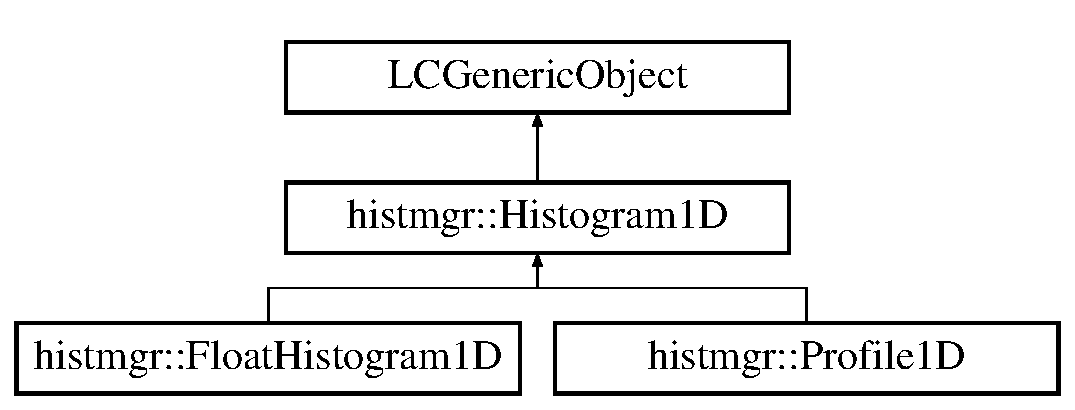
\includegraphics[height=3.000000cm]{classhistmgr_1_1Histogram1D}
\end{center}
\end{figure}
\subsection*{Public Member Functions}
\begin{DoxyCompactItemize}
\item 
virtual int {\bf id} () const \label{classhistmgr_1_1Histogram1D_a524540a72e8d5f19fa3fcaec65610b0c}

\begin{DoxyCompactList}\small\item\em Return the id of the underlying L\-C\-Generic\-Object\-Impl. \end{DoxyCompactList}\item 
U\-Int\-\_\-t {\bf first\-Bin\-Index} () const \label{classhistmgr_1_1Histogram1D_acda829dea1a315f62e4618beecac3409}

\begin{DoxyCompactList}\small\item\em Return the index of the first bin not below the minimum axis value. \end{DoxyCompactList}\item 
U\-Int\-\_\-t {\bf last\-Bin\-Index} () const \label{classhistmgr_1_1Histogram1D_a21cfe7d0e489202dcd0138da20349f74}

\begin{DoxyCompactList}\small\item\em Return the index of the last bin not above the maximum axis value. \end{DoxyCompactList}\item 
U\-Int\-\_\-t {\bf underflow\-Bin\-Index} () const \label{classhistmgr_1_1Histogram1D_a444200d12e95077d3ff93451ac9d51f5}

\begin{DoxyCompactList}\small\item\em Return the index of the bin below the minimum axis value (underflow bin). \end{DoxyCompactList}\item 
U\-Int\-\_\-t {\bf overflow\-Bin\-Index} () const \label{classhistmgr_1_1Histogram1D_a2f68dc59449bb4242e113cd62365acc7}

\begin{DoxyCompactList}\small\item\em Return the index of the bin above the maximum axis value (overflow bin). \end{DoxyCompactList}\item 
U\-Int\-\_\-t {\bf n\-Bins} () const \label{classhistmgr_1_1Histogram1D_aabad63ec43eec6b9ec5250b409d50ef9}

\begin{DoxyCompactList}\small\item\em Return the number of bins. \end{DoxyCompactList}\item 
Float\-\_\-t {\bf x\-Min} () const \label{classhistmgr_1_1Histogram1D_a008b31ebefbd1149cc906975b7025996}

\begin{DoxyCompactList}\small\item\em The minimum axis value (lower edge of the histogram range). \end{DoxyCompactList}\item 
Float\-\_\-t {\bf x\-Max} () const \label{classhistmgr_1_1Histogram1D_aa1f98c2b6d73bcf1c0209f055d283c1b}

\begin{DoxyCompactList}\small\item\em The maximum axis value (upper edge of the histogram range). \end{DoxyCompactList}\item 
Float\-\_\-t {\bf bin\-Center} (U\-Int\-\_\-t bin\-\_\-index) const \label{classhistmgr_1_1Histogram1D_a74f37e72347aca0eb04085fe98b063da}

\begin{DoxyCompactList}\small\item\em Return the axis value of the centre of the given bin. \end{DoxyCompactList}\item 
Float\-\_\-t {\bfseries bin\-Low\-Edge} (U\-Int\-\_\-t bin\-\_\-index) const \label{classhistmgr_1_1Histogram1D_a5cc5aa3eba6272c03a6147b860a8b8e3}

\item 
Float\-\_\-t {\bf bin\-Width} (U\-Int\-\_\-t) const \label{classhistmgr_1_1Histogram1D_a7c1fa00271d1776d054a8c337a56fd82}

\begin{DoxyCompactList}\small\item\em Return the width of the given bin. \end{DoxyCompactList}\item 
U\-Int\-\_\-t {\bf calice\-\_\-id} ()\label{classhistmgr_1_1Histogram1D_acd92f881bf13e97509720ddbb0063b4b}

\begin{DoxyCompactList}\small\item\em Return the id of the histogram. \end{DoxyCompactList}\item 
Double\-\_\-t {\bf entries} () const \label{classhistmgr_1_1Histogram1D_a22623460729f7e584282802d7320839c}

\begin{DoxyCompactList}\small\item\em Return the number of entries of the histogram. \end{DoxyCompactList}\end{DoxyCompactItemize}
\subsection*{Protected Member Functions}
\begin{DoxyCompactItemize}
\item 
{\bfseries Histogram1\-D} (lcio\-::\-L\-C\-Object $\ast$a\-\_\-obj)\label{classhistmgr_1_1Histogram1D_af17dcdb05c069e893c014c25581946ad}

\item 
void {\bf add\-To\-Entries} (Double\-\_\-t weight)
\begin{DoxyCompactList}\small\item\em Add weight to the number of entries. \end{DoxyCompactList}\item 
int {\bfseries get\-N\-Int} () const \label{classhistmgr_1_1Histogram1D_a9f6771b7dfedce460ba615330db8f3ee}

\item 
int {\bfseries get\-N\-Float} () const \label{classhistmgr_1_1Histogram1D_a7df3b9136394f70dfe46e7465195134d}

\item 
int {\bfseries get\-N\-Double} () const \label{classhistmgr_1_1Histogram1D_a40876551abee3a5cb68f7406024cb6fd}

\item 
int {\bfseries get\-Int\-Val} (int index) const \label{classhistmgr_1_1Histogram1D_a460737d4258f5bb33b2cda3a435c4fb6}

\item 
float {\bfseries get\-Float\-Val} (int index) const \label{classhistmgr_1_1Histogram1D_a1a71d70f6c054b7cbab67ca04364f271}

\item 
double {\bfseries get\-Double\-Val} (int index) const \label{classhistmgr_1_1Histogram1D_a6e76a153525e974912e904a37c00c217}

\item 
bool {\bfseries is\-Fixed\-Size} () const \label{classhistmgr_1_1Histogram1D_ae009c17abdb58995d8777a0ff4af75cd}

\item 
const std\-::string {\bfseries get\-Type\-Name} () const \label{classhistmgr_1_1Histogram1D_a89c9f20156c75f61297a5e4901e49936}

\item 
const std\-::string {\bfseries get\-Data\-Description} () const \label{classhistmgr_1_1Histogram1D_aebfe652d6212c54e784489b13490853b}

\item 
void {\bf set\-Binning} (const {\bf Hist\-Par} \&bins)\label{classhistmgr_1_1Histogram1D_aa8334230aef792b7cbec7dd4ff8e039b}

\begin{DoxyCompactList}\small\item\em Store the binning of the histogram. \end{DoxyCompactList}\item 
U\-Int\-\_\-t {\bf bin\-Index} (Float\-\_\-t value) const \label{classhistmgr_1_1Histogram1D_a42a8f19a46ae2582c1a913bc5c765831}

\begin{DoxyCompactList}\small\item\em Calculate and return the bin index for the given axis value. \end{DoxyCompactList}\item 
lcio\-::\-L\-C\-Generic\-Object\-Impl $\ast$ {\bfseries obj} ()\label{classhistmgr_1_1Histogram1D_a87ce666baabddda16f4c1f22f57873d4}

\item 
const lcio\-::\-L\-C\-Generic\-Object\-Impl $\ast$ {\bfseries obj} () const \label{classhistmgr_1_1Histogram1D_a2eea045a1d4a53f4ab193a93781bd3bf}

\end{DoxyCompactItemize}
\subsection*{Protected Attributes}
\begin{DoxyCompactItemize}
\item 
lcio\-::\-L\-C\-Generic\-Object\-Impl $\ast$ {\bfseries \-\_\-obj}\label{classhistmgr_1_1Histogram1D_ac54ece569a39b15d5f29d685a08d161c}

\item 
bool {\bfseries \-\_\-created\-Object}\label{classhistmgr_1_1Histogram1D_a4a49b47ef95c3733cd57cdc675227791}

\end{DoxyCompactItemize}
\subsection*{Static Protected Attributes}
\begin{DoxyCompactItemize}
\item 
static const std\-::string {\bfseries \-\_\-\-\_\-type\-Name} =\char`\"{}Histogram1\-D\char`\"{}\label{classhistmgr_1_1Histogram1D_a99612636650ea16a94249d8a068f3439}

\item 
static const std\-::string {\bfseries \-\_\-\-\_\-description} =\char`\"{}Histogram1\-D\char`\"{}\label{classhistmgr_1_1Histogram1D_aaa4194c1a6de8d9eb955a191edfd125c}

\end{DoxyCompactItemize}


\subsection{Detailed Description}
Equidistant binned 1\-D histogram without data container. 

The histogram is kept very simple and does not make use of virtual functions in order to be very fast. Note\-: the histogram does not have a data container. A usable histogram is the \doxyref{Float\-Histogram1\-D}{p.}{classhistmgr_1_1FloatHistogram1D}. 

Definition at line 27 of file Histogram1\-D.\-hh.



\subsection{Member Function Documentation}
\index{histmgr\-::\-Histogram1\-D@{histmgr\-::\-Histogram1\-D}!add\-To\-Entries@{add\-To\-Entries}}
\index{add\-To\-Entries@{add\-To\-Entries}!histmgr::Histogram1D@{histmgr\-::\-Histogram1\-D}}
\subsubsection[{add\-To\-Entries}]{\setlength{\rightskip}{0pt plus 5cm}void histmgr\-::\-Histogram1\-D\-::add\-To\-Entries (
\begin{DoxyParamCaption}
\item[{Double\-\_\-t}]{weight}
\end{DoxyParamCaption}
)\hspace{0.3cm}{\ttfamily [inline]}, {\ttfamily [protected]}}\label{classhistmgr_1_1Histogram1D_aa49e6a8526463293e4ca43c279ce3e86}


Add weight to the number of entries. 

Weight is usually 1, but may be a fractional value in the interval (0,oo). N\-O\-T\-E\-: No range check of the weight is performed. 

Definition at line 120 of file Histogram1\-D.\-hh.



References entries().



The documentation for this class was generated from the following files\-:\begin{DoxyCompactItemize}
\item 
Histogram1\-D.\-hh\item 
Histogram1\-D.\-cc\end{DoxyCompactItemize}

\section{histmgr\-:\-:Histogram2\-D Class Reference}
\label{classhistmgr_1_1Histogram2D}\index{histmgr\-::\-Histogram2\-D@{histmgr\-::\-Histogram2\-D}}
Inheritance diagram for histmgr\-:\-:Histogram2\-D\-:\begin{figure}[H]
\begin{center}
\leavevmode
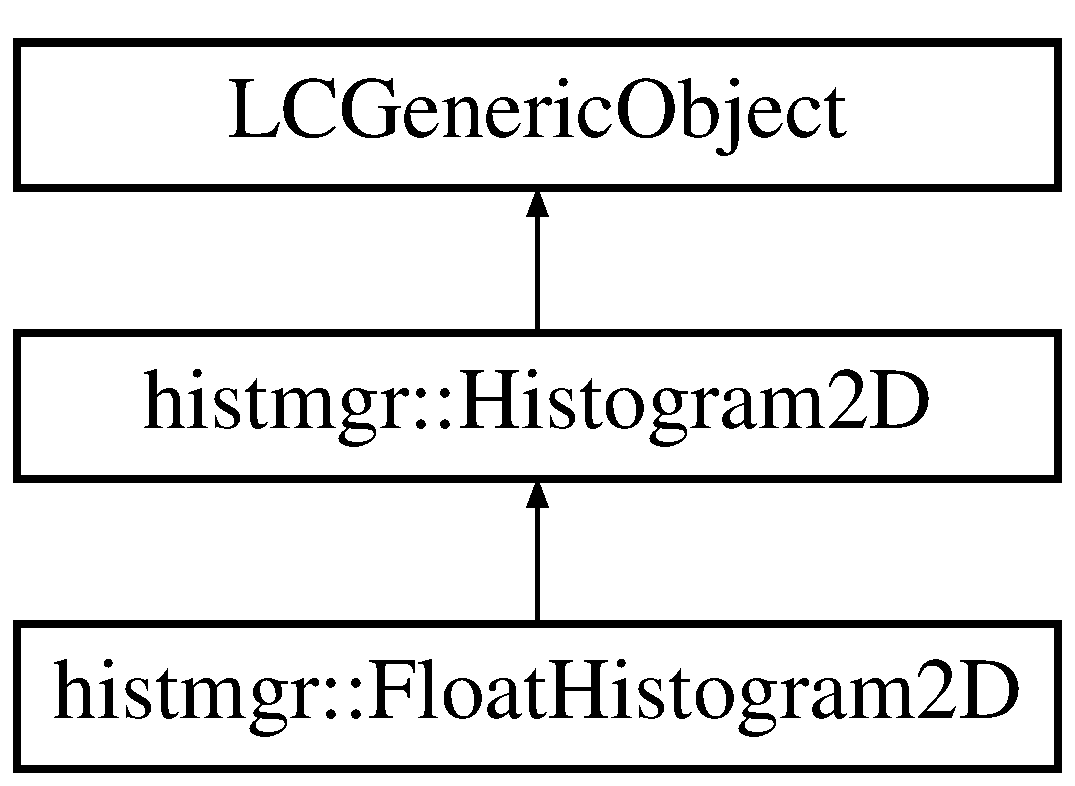
\includegraphics[height=3.000000cm]{classhistmgr_1_1Histogram2D}
\end{center}
\end{figure}
\subsection*{Public Member Functions}
\begin{DoxyCompactItemize}
\item 
virtual int {\bf id} () const \label{classhistmgr_1_1Histogram2D_a76da2e4085a49feffbcf45457b55634d}

\begin{DoxyCompactList}\small\item\em Return the id of the underlying L\-C\-Generic\-Object\-Impl. \end{DoxyCompactList}\item 
U\-Int\-\_\-t {\bfseries x\-First\-Bin\-Index} () const \label{classhistmgr_1_1Histogram2D_abf70969b4294719fb4c480d2485b6f02}

\item 
U\-Int\-\_\-t {\bfseries x\-Last\-Bin\-Index} () const \label{classhistmgr_1_1Histogram2D_aa816778d15e7eb3b9ab2affa02ceae0c}

\item 
U\-Int\-\_\-t {\bfseries y\-First\-Bin\-Index} () const \label{classhistmgr_1_1Histogram2D_a3e3a5b7d3d907c8be90ca562a2ea832c}

\item 
U\-Int\-\_\-t {\bfseries y\-Last\-Bin\-Index} () const \label{classhistmgr_1_1Histogram2D_af850544bb3c6d6a278e518a4ba7c5146}

\item 
U\-Int\-\_\-t {\bfseries x\-Underflow\-Bin\-Index} () const \label{classhistmgr_1_1Histogram2D_ac6e27ddf89725fe49eeaf1568c8024c2}

\item 
U\-Int\-\_\-t {\bfseries x\-Overflow\-Bin\-Index} () const \label{classhistmgr_1_1Histogram2D_a6eb4490be5315d81c344a6e17d6cd1f6}

\item 
U\-Int\-\_\-t {\bfseries y\-Underflow\-Bin\-Index} () const \label{classhistmgr_1_1Histogram2D_a09627b05e21e4544e621efc423936c81}

\item 
U\-Int\-\_\-t {\bfseries y\-Overflow\-Bin\-Index} () const \label{classhistmgr_1_1Histogram2D_a994f0c6eaf2179019ad0202282b73c80}

\item 
U\-Int\-\_\-t {\bfseries x\-N\-Bins} () const \label{classhistmgr_1_1Histogram2D_a955bc09c119a9ccf995c40d055556250}

\item 
Float\-\_\-t {\bfseries x\-Min} () const \label{classhistmgr_1_1Histogram2D_a9c5990884d2b038d94e56640e8f70a12}

\item 
Float\-\_\-t {\bfseries x\-Max} () const \label{classhistmgr_1_1Histogram2D_a96a6a6d6dff2e8fe03a368c462c88952}

\item 
U\-Int\-\_\-t {\bfseries y\-N\-Bins} () const \label{classhistmgr_1_1Histogram2D_a948a659fdd1a04946da319aacf809a75}

\item 
Float\-\_\-t {\bfseries y\-Min} () const \label{classhistmgr_1_1Histogram2D_acbe0f9156f69af35e7701796424efc57}

\item 
Float\-\_\-t {\bfseries y\-Max} () const \label{classhistmgr_1_1Histogram2D_a6e170388b9fe540e4553b2056691045d}

\item 
Float\-\_\-t {\bfseries x\-Bin\-Center} (U\-Int\-\_\-t bin\-\_\-index)\label{classhistmgr_1_1Histogram2D_a34240deb29b7af10792e82ab00a1ba96}

\item 
Float\-\_\-t {\bfseries x\-Bin\-Low\-Edge} (U\-Int\-\_\-t bin\-\_\-index)\label{classhistmgr_1_1Histogram2D_a86e526af29aa24c0a0486f84d800fecf}

\item 
Float\-\_\-t {\bfseries x\-Bin\-Width} (U\-Int\-\_\-t)\label{classhistmgr_1_1Histogram2D_ac8fd83fa10fc3468361e4d2e56d50442}

\item 
Float\-\_\-t {\bfseries y\-Bin\-Center} (U\-Int\-\_\-t bin\-\_\-index)\label{classhistmgr_1_1Histogram2D_afed2edc77e0353c1366dc555f49e22c0}

\item 
Float\-\_\-t {\bfseries y\-Bin\-Low\-Edge} (U\-Int\-\_\-t bin\-\_\-index)\label{classhistmgr_1_1Histogram2D_a3084d9ba1b47a865c36745fd19c7e7d3}

\item 
Float\-\_\-t {\bfseries y\-Bin\-Width} (U\-Int\-\_\-t)\label{classhistmgr_1_1Histogram2D_acc19b4a6e328acb6899de0c7504e2343}

\item 
U\-Int\-\_\-t {\bfseries calice\-\_\-id} ()\label{classhistmgr_1_1Histogram2D_aa6ea5c5bb5ff2b0fc7f6a8e9a5f3e625}

\item 
Double\-\_\-t {\bfseries entries} () const \label{classhistmgr_1_1Histogram2D_abb7d72e42edb6531399b10a91794382a}

\item 
void {\bfseries add\-To\-Entries} (Double\-\_\-t weight)\label{classhistmgr_1_1Histogram2D_a98f58e8e6d67a3430fb9047552c95b17}

\item 
int {\bfseries get\-N\-Int} () const \label{classhistmgr_1_1Histogram2D_a89e0f3cdde009efa4214734afb619960}

\item 
int {\bfseries get\-N\-Float} () const \label{classhistmgr_1_1Histogram2D_acfe071923f9d990ec61568fd8c6e72f5}

\item 
int {\bfseries get\-N\-Double} () const \label{classhistmgr_1_1Histogram2D_aa3292dae2356c865b67dc62fdd1abfb5}

\item 
int {\bfseries get\-Int\-Val} (int index) const \label{classhistmgr_1_1Histogram2D_a39f56d711ed8d5921f7662d038ead2d1}

\item 
float {\bfseries get\-Float\-Val} (int index) const \label{classhistmgr_1_1Histogram2D_ab2fb60d75ad648ef7cdc259553a5c578}

\item 
double {\bfseries get\-Double\-Val} (int index) const \label{classhistmgr_1_1Histogram2D_a0ad3f76facb8a045e4ce6a0ac730e72a}

\item 
bool {\bfseries is\-Fixed\-Size} () const \label{classhistmgr_1_1Histogram2D_a9062278e2daa5a095356fbf331b3b921}

\item 
const std\-::string {\bfseries get\-Type\-Name} () const \label{classhistmgr_1_1Histogram2D_aae1137af1c5d111b441b80d74ef606ba}

\item 
const std\-::string {\bfseries get\-Data\-Description} () const \label{classhistmgr_1_1Histogram2D_aa9b8b32e5080f678d0b7e876c54ba453}

\end{DoxyCompactItemize}
\subsection*{Protected Member Functions}
\begin{DoxyCompactItemize}
\item 
{\bfseries Histogram2\-D} (lcio\-::\-L\-C\-Object $\ast$a\-\_\-obj)\label{classhistmgr_1_1Histogram2D_ade05eeddf75a2b5e341194c77fb9d101}

\item 
void {\bfseries set\-Binning} (const {\bf Hist\-Par} \&x\-\_\-bins, const {\bf Hist\-Par} \&y\-\_\-bins)\label{classhistmgr_1_1Histogram2D_a5599afe22a258e379309225ba43b8fd3}

\item 
void {\bfseries set\-Xto\-Bins} ()\label{classhistmgr_1_1Histogram2D_a56dc039a37aa7bf88366e72e38535d9b}

\item 
void {\bfseries set\-Yto\-Bins} ()\label{classhistmgr_1_1Histogram2D_adfafff46dede8944cb1a7569e864a1a2}

\item 
U\-Int\-\_\-t {\bfseries x\-Bin\-Index} (Float\-\_\-t value) const \label{classhistmgr_1_1Histogram2D_af1dab9a3f3ef0c7f015934014fbb6118}

\item 
U\-Int\-\_\-t {\bfseries y\-Bin\-Index} (Float\-\_\-t value) const \label{classhistmgr_1_1Histogram2D_abc60652d0255c12f81b5ac270f28e744}

\item 
U\-Int\-\_\-t {\bfseries get\-Container\-Size} () const \label{classhistmgr_1_1Histogram2D_adc5826e91c1e1b571fb9a1a0c3cbdadf}

\item 
lcio\-::\-L\-C\-Generic\-Object\-Impl $\ast$ {\bfseries obj} ()\label{classhistmgr_1_1Histogram2D_a858dc3152e69254166a94bd9da833be3}

\item 
const lcio\-::\-L\-C\-Generic\-Object\-Impl $\ast$ {\bfseries obj} () const \label{classhistmgr_1_1Histogram2D_a727d937e500b3a05a8c1d9d197198bfb}

\end{DoxyCompactItemize}
\subsection*{Protected Attributes}
\begin{DoxyCompactItemize}
\item 
lcio\-::\-L\-C\-Generic\-Object\-Impl $\ast$ {\bfseries \-\_\-obj}\label{classhistmgr_1_1Histogram2D_ac665536e5e1b13a7482018306b70424d}

\item 
bool {\bfseries \-\_\-created\-Object}\label{classhistmgr_1_1Histogram2D_a5e72c0d4241393ceda4f54a441cc9d72}

\item 
Double\-\_\-t {\bfseries \-\_\-x\-To\-Bin}\label{classhistmgr_1_1Histogram2D_aee7de840bafcc507ff2cf1165ad97c53}

\item 
Double\-\_\-t {\bfseries \-\_\-y\-To\-Bin}\label{classhistmgr_1_1Histogram2D_af65c161601e9290bc97be2f8debbecd8}

\end{DoxyCompactItemize}
\subsection*{Static Protected Attributes}
\begin{DoxyCompactItemize}
\item 
static const std\-::string {\bfseries \-\_\-\-\_\-type\-Name} =\char`\"{}Histogram2\-D\char`\"{}\label{classhistmgr_1_1Histogram2D_ae180a84a85576bfe6648db62f402d42e}

\item 
static const std\-::string {\bfseries \-\_\-\-\_\-description} =\char`\"{}Histogram2\-D\char`\"{}\label{classhistmgr_1_1Histogram2D_a0d54044cca0f5111309d9a22481b6236}

\end{DoxyCompactItemize}


\subsection{Detailed Description}


Definition at line 22 of file Histogram2\-D.\-hh.



The documentation for this class was generated from the following files\-:\begin{DoxyCompactItemize}
\item 
Histogram2\-D.\-hh\item 
Histogram2\-D.\-cc\end{DoxyCompactItemize}

\section{histmgr\-:\-:Histogram2\-D\-Collection\-\_\-t Class Reference}
\label{classhistmgr_1_1Histogram2DCollection__t}\index{histmgr\-::\-Histogram2\-D\-Collection\-\_\-t@{histmgr\-::\-Histogram2\-D\-Collection\-\_\-t}}


One or two dimensional collection of histograms.  




{\ttfamily \#include $<$Histogram2\-D\-Collection\-\_\-t.\-hh$>$}

Inheritance diagram for histmgr\-:\-:Histogram2\-D\-Collection\-\_\-t\-:\begin{figure}[H]
\begin{center}
\leavevmode
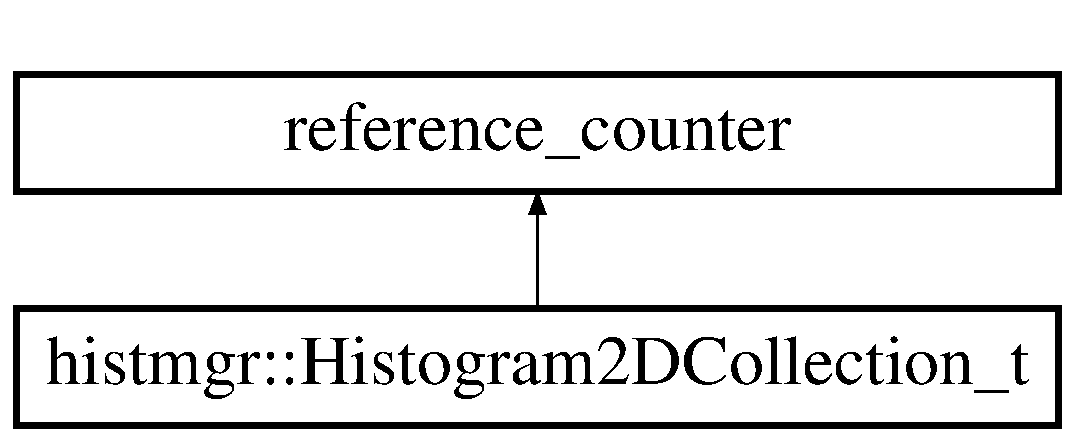
\includegraphics[height=2.000000cm]{classhistmgr_1_1Histogram2DCollection__t}
\end{center}
\end{figure}
\subsection*{Public Member Functions}
\begin{DoxyCompactItemize}
\item 
{\bf Histogram2\-D\-Collection\-\_\-t} (const std\-::string \&collection\-\_\-name, const E\-V\-E\-N\-T\-::\-String\-Vec \&name\-\_\-list, U\-Int\-\_\-t n\-\_\-hist, const {\bf Hist\-Par} \&x\-\_\-par, const {\bf Hist\-Par} \&y\-\_\-par) noexcept(false)
\begin{DoxyCompactList}\small\item\em Create a collection of histograms which will have the same binning and the same name (except of a numeric extension). \end{DoxyCompactList}\item 
{\bf Histogram2\-D\-Collection\-\_\-t} (const std\-::string \&collection\-\_\-name, const E\-V\-E\-N\-T\-::\-String\-Vec \&name\-\_\-list, const lcio\-::\-Int\-Vec \&n\-\_\-hist\-\_\-list, const {\bf Hist\-Par} \&x\-\_\-par, const {\bf Hist\-Par} \&y\-\_\-par)
\begin{DoxyCompactList}\small\item\em Create a collection of histograms which will have the same binning and the same name (except of a numeric extension). \end{DoxyCompactList}\item 
{\bf Histogram2\-D\-Collection\-\_\-t} (lcio\-::\-L\-C\-Collection $\ast$histograms, lcio\-::\-Int\-Vec $\ast$indices)
\item 
{\bf Histogram2\-D\-Collection\-\_\-t} (lcio\-::\-L\-C\-Collection $\ast$histograms)
\begin{DoxyCompactList}\small\item\em Create a histogram collection from lcio collection. \end{DoxyCompactList}\item 
{\bf Histogram2\-D\-Collection\-\_\-t} (const {\bf Histogram2\-D\-Collection\-\_\-t} \&a)\label{classhistmgr_1_1Histogram2DCollection__t_a2f6e961d72d471440615a4673d3f2de4}

\begin{DoxyCompactList}\small\item\em copy constructor. \end{DoxyCompactList}\item 
{\bf Histogram2\-D\-Collection\-\_\-t} ()\label{classhistmgr_1_1Histogram2DCollection__t_aa51815c63839cc73273232df3cc53d91}

\begin{DoxyCompactList}\small\item\em Default constructor. \end{DoxyCompactList}\item 
void {\bf delete\-Collection} ()\label{classhistmgr_1_1Histogram2DCollection__t_a3dc0a213db50d0a0eb58441ce29875c6}

\begin{DoxyCompactList}\small\item\em delete the histogram collection and the index array This method exists instead of a destrctor to prevent copying the arrays (F\-I\-X\-M\-E) \end{DoxyCompactList}\item 
void {\bfseries delete\-Shared\-Storage} ()\label{classhistmgr_1_1Histogram2DCollection__t_aa8f4d87ede0c6bbcc3f22cea2dca2f3f}

\item 
lcio\-::\-L\-C\-Collection $\ast$ {\bf create\-Histograms} (const std\-::string \&collection\-\_\-name, const E\-V\-E\-N\-T\-::\-String\-Vec \&name\-\_\-list, U\-Int\-\_\-t n\-\_\-hist, const {\bf Hist\-Par} \&x\-\_\-par, const {\bf Hist\-Par} \&y\-\_\-par) noexcept(false)
\begin{DoxyCompactList}\small\item\em create several histograms which will have the same binning and the same name (except of a numeric extension). \end{DoxyCompactList}\item 
lcio\-::\-L\-C\-Collection $\ast$ {\bf create\-Histograms} (const std\-::string \&collection\-\_\-name, const E\-V\-E\-N\-T\-::\-String\-Vec \&name\-\_\-list, const lcio\-::\-Int\-Vec \&n\-\_\-hist\-\_\-list, const {\bf Hist\-Par} \&x\-\_\-par, const {\bf Hist\-Par} \&y\-\_\-par) noexcept(false)
\begin{DoxyCompactList}\small\item\em create several histograms which will have the same binning and the same name (except of a numeric extension). \end{DoxyCompactList}\item 
lcio\-::\-L\-C\-Collection $\ast$ {\bf collection} ()
\begin{DoxyCompactList}\small\item\em get the unique group id \end{DoxyCompactList}\item 
const lcio\-::\-L\-C\-Collection $\ast$ {\bf collection} () const 
\begin{DoxyCompactList}\small\item\em get the collection of histograms (read only). \end{DoxyCompactList}\item 
U\-Int\-\_\-t {\bf n} () const \label{classhistmgr_1_1Histogram2DCollection__t_a4aa15bd76ec1a055afe867e0a59daab6}

\begin{DoxyCompactList}\small\item\em get the number of histograms in the one dimensional collection. \end{DoxyCompactList}\item 
bool {\bf is2\-D} () const \label{classhistmgr_1_1Histogram2DCollection__t_a915231d0006aa618929865be0717d676}

\begin{DoxyCompactList}\small\item\em Return true if the histogram collection is two instead of one diemensional. \end{DoxyCompactList}\item 
U\-Int\-\_\-t {\bf n\-Major} () const \label{classhistmgr_1_1Histogram2DCollection__t_a7d589f32e849ee6c2ff62d22f67e596b}

\begin{DoxyCompactList}\small\item\em get the number of histograms in the one dimensional collection. \end{DoxyCompactList}\item 
U\-Int\-\_\-t {\bf n\-Minor} (U\-Int\-\_\-t major\-\_\-index) const \label{classhistmgr_1_1Histogram2DCollection__t_af72ed2b8399f39439bc2b232820696f2}

\begin{DoxyCompactList}\small\item\em get the number of histograms in the one dimensional collection. \end{DoxyCompactList}\item 
const {\bf Float\-Histogram2\-D} $\ast$ {\bf histogram} (U\-Int\-\_\-t index) const \label{classhistmgr_1_1Histogram2DCollection__t_abd1f0ccdbc83f9f6fbbea239162d99d8}

\begin{DoxyCompactList}\small\item\em Get one histogram of the collection (read only). \end{DoxyCompactList}\item 
{\bf Float\-Histogram2\-D} $\ast$ {\bf histogram} (U\-Int\-\_\-t index)\label{classhistmgr_1_1Histogram2DCollection__t_afc8d2ea4e42d5e6cf283792b819d95c1}

\begin{DoxyCompactList}\small\item\em Get one histogram of the collection. \end{DoxyCompactList}\item 
{\bf Float\-Histogram2\-D} $\ast$ {\bf histogram} (U\-Int\-\_\-t major\-\_\-index, U\-Int\-\_\-t minor\-\_\-index)\label{classhistmgr_1_1Histogram2DCollection__t_a182a4f9dd876337a00a5e57f8358555f}

\begin{DoxyCompactList}\small\item\em Get one histogram of the collection which is organised as a two dimensional array. \end{DoxyCompactList}\item 
const {\bf Float\-Histogram2\-D} $\ast$ {\bf histogram} (U\-Int\-\_\-t major\-\_\-index, U\-Int\-\_\-t minor\-\_\-index) const \label{classhistmgr_1_1Histogram2DCollection__t_a3ea359f9713ea66fe5ceaf0b82539776}

\begin{DoxyCompactList}\small\item\em Get one histogram of the collection which is organised as a two dimensional array (read only). \end{DoxyCompactList}\item 
const std\-::string \& {\bf get\-Name} (U\-Int\-\_\-t major\-\_\-index) const 
\begin{DoxyCompactList}\small\item\em Get the name of the specified element of the histogram collection. \end{DoxyCompactList}\end{DoxyCompactItemize}
\subsection*{Static Protected Attributes}
\begin{DoxyCompactItemize}
\item 
static const std\-::string {\bfseries \-\_\-\-\_\-histogram\-Name\-Parameter\-Name}\label{classhistmgr_1_1Histogram2DCollection__t_a9c9c12ef5e660181a010b4e9e3543e8d}

\end{DoxyCompactItemize}
\subsection*{Private Member Functions}
\begin{DoxyCompactItemize}
\item 
void {\bf copy\-Names} () const 
\begin{DoxyCompactList}\small\item\em Copy the names from the collection to an accessible vector. \end{DoxyCompactList}\end{DoxyCompactItemize}
\subsection*{Private Attributes}
\begin{DoxyCompactItemize}
\item 
lcio\-::\-L\-C\-Collection $\ast$ {\bf \-\_\-histogram\-Col}\label{classhistmgr_1_1Histogram2DCollection__t_a935072d41133e1922cfa3372a859bda8}

\begin{DoxyCompactList}\small\item\em the histogram collection \end{DoxyCompactList}\item 
lcio\-::\-Int\-Vec $\ast$ {\bf \-\_\-major\-Index}
\begin{DoxyCompactList}\small\item\em optional list of offset to form a two dimensional array out of the list. \end{DoxyCompactList}\item 
lcio\-::\-String\-Vec {\bf \-\_\-name\-List}
\begin{DoxyCompactList}\small\item\em A vector which contains one name for all histograms of the collection or a name for each element. \end{DoxyCompactList}\end{DoxyCompactItemize}
\subsection*{Static Private Attributes}
\begin{DoxyCompactItemize}
\item 
static const std\-::string {\bfseries \-\_\-\-\_\-major\-Index\-Parameter\-Name}\label{classhistmgr_1_1Histogram2DCollection__t_aded8e87a24b7ee1bd042c0bb352fdf1d}

\item 
static const std\-::string {\bfseries \-\_\-\-\_\-default\-Histogram\-Name}\label{classhistmgr_1_1Histogram2DCollection__t_ac482b686014b906aa2be8da6a4ca9844}

\end{DoxyCompactItemize}
\subsection*{Friends}
\begin{DoxyCompactItemize}
\item 
class {\bfseries Hist\-Mgr}\label{classhistmgr_1_1Histogram2DCollection__t_a3cc85db784d7651390e41024125eb3a0}

\end{DoxyCompactItemize}
\subsection*{Additional Inherited Members}


\subsection{Detailed Description}
One or two dimensional collection of histograms. 

Definition at line 16 of file Histogram2\-D\-Collection\-\_\-t.\-hh.



\subsection{Constructor \& Destructor Documentation}
\index{histmgr\-::\-Histogram2\-D\-Collection\-\_\-t@{histmgr\-::\-Histogram2\-D\-Collection\-\_\-t}!Histogram2\-D\-Collection\-\_\-t@{Histogram2\-D\-Collection\-\_\-t}}
\index{Histogram2\-D\-Collection\-\_\-t@{Histogram2\-D\-Collection\-\_\-t}!histmgr::Histogram2DCollection_t@{histmgr\-::\-Histogram2\-D\-Collection\-\_\-t}}
\subsubsection[{Histogram2\-D\-Collection\-\_\-t}]{\setlength{\rightskip}{0pt plus 5cm}histmgr\-::\-Histogram2\-D\-Collection\-\_\-t\-::\-Histogram2\-D\-Collection\-\_\-t (
\begin{DoxyParamCaption}
\item[{const std\-::string \&}]{collection\-\_\-name, }
\item[{const E\-V\-E\-N\-T\-::\-String\-Vec \&}]{name\-\_\-list, }
\item[{U\-Int\-\_\-t}]{n\-\_\-hist, }
\item[{const {\bf Hist\-Par} \&}]{x\-\_\-par, }
\item[{const {\bf Hist\-Par} \&}]{y\-\_\-par}
\end{DoxyParamCaption}
)\hspace{0.3cm}{\ttfamily [inline]}, {\ttfamily [noexcept]}}\label{classhistmgr_1_1Histogram2DCollection__t_a56b6cbce7bb7259f55b92f72db00c9cf}


Create a collection of histograms which will have the same binning and the same name (except of a numeric extension). 


\begin{DoxyParams}{Parameters}
{\em collection\-\_\-name} & the name of the histogram collection \\
\hline
{\em name\-\_\-list} & a vector containing the names of the histograms whose length is either equals n\-\_\-hist or is zero. In the latter case the collection name is used for the all histograms. \\
\hline
{\em n\-\_\-hist} & the number of histograms to be created \\
\hline
{\em x\-\_\-par} & the binning of the x-\/axis of the histogram \\
\hline
{\em y\-\_\-par} & the binning of the y-\/axis of the histogram\\
\hline
\end{DoxyParams}
The histograms are only written to a file if the histogram group, to which this histogram belongs, is assigned to a file (\doxyref{histmgr\-::\-Hist\-Mgr\-::assign\-File\-Name}{p.}{classhistmgr_1_1HistMgr_a20e3c96a8ba6175c8036918ca7acb1e2}). 

Definition at line 33 of file Histogram2\-D\-Collection\-\_\-t.\-hh.



References create\-Histograms().

\index{histmgr\-::\-Histogram2\-D\-Collection\-\_\-t@{histmgr\-::\-Histogram2\-D\-Collection\-\_\-t}!Histogram2\-D\-Collection\-\_\-t@{Histogram2\-D\-Collection\-\_\-t}}
\index{Histogram2\-D\-Collection\-\_\-t@{Histogram2\-D\-Collection\-\_\-t}!histmgr::Histogram2DCollection_t@{histmgr\-::\-Histogram2\-D\-Collection\-\_\-t}}
\subsubsection[{Histogram2\-D\-Collection\-\_\-t}]{\setlength{\rightskip}{0pt plus 5cm}histmgr\-::\-Histogram2\-D\-Collection\-\_\-t\-::\-Histogram2\-D\-Collection\-\_\-t (
\begin{DoxyParamCaption}
\item[{const std\-::string \&}]{collection\-\_\-name, }
\item[{const E\-V\-E\-N\-T\-::\-String\-Vec \&}]{name\-\_\-list, }
\item[{const lcio\-::\-Int\-Vec \&}]{n\-\_\-hist\-\_\-list, }
\item[{const {\bf Hist\-Par} \&}]{x\-\_\-par, }
\item[{const {\bf Hist\-Par} \&}]{y\-\_\-par}
\end{DoxyParamCaption}
)\hspace{0.3cm}{\ttfamily [inline]}}\label{classhistmgr_1_1Histogram2DCollection__t_a787b3b7485747847457337b7e138f0ed}


Create a collection of histograms which will have the same binning and the same name (except of a numeric extension). 


\begin{DoxyParams}{Parameters}
{\em collection\-\_\-name} & the of the histogram collection \\
\hline
{\em name\-\_\-list} & a vector containing the names of the histograms whose length is either equals n\-\_\-hist or is zero. In the latter case the collection name is used for the all histograms. \\
\hline
{\em n\-\_\-hist\-\_\-list} & the number of histograms to be created \\
\hline
{\em x\-\_\-par} & the binning of the x-\/axis of the histogram \\
\hline
{\em y\-\_\-par} & the binning of the y-\/axis of the histogram\\
\hline
\end{DoxyParams}
\begin{DoxyReturn}{Returns}
pointer to the histogram collection
\end{DoxyReturn}
The histograms are only written to a file if the histogram group, to which this histogram belongs, is assigned to a file (\doxyref{histmgr\-::\-Hist\-Mgr\-::assign\-File\-Name}{p.}{classhistmgr_1_1HistMgr_a20e3c96a8ba6175c8036918ca7acb1e2}). 

Definition at line 60 of file Histogram2\-D\-Collection\-\_\-t.\-hh.



References create\-Histograms().

\index{histmgr\-::\-Histogram2\-D\-Collection\-\_\-t@{histmgr\-::\-Histogram2\-D\-Collection\-\_\-t}!Histogram2\-D\-Collection\-\_\-t@{Histogram2\-D\-Collection\-\_\-t}}
\index{Histogram2\-D\-Collection\-\_\-t@{Histogram2\-D\-Collection\-\_\-t}!histmgr::Histogram2DCollection_t@{histmgr\-::\-Histogram2\-D\-Collection\-\_\-t}}
\subsubsection[{Histogram2\-D\-Collection\-\_\-t}]{\setlength{\rightskip}{0pt plus 5cm}histmgr\-::\-Histogram2\-D\-Collection\-\_\-t\-::\-Histogram2\-D\-Collection\-\_\-t (
\begin{DoxyParamCaption}
\item[{lcio\-::\-L\-C\-Collection $\ast$}]{histograms, }
\item[{lcio\-::\-Int\-Vec $\ast$}]{indices}
\end{DoxyParamCaption}
)\hspace{0.3cm}{\ttfamily [inline]}}\label{classhistmgr_1_1Histogram2DCollection__t_adb283f18b76bde0d93371c93e2ab372d}

\begin{DoxyParams}{Parameters}
{\em histograms} & the linearised one or two dimensional collection of histograms \\
\hline
{\em indices} & optional list of indicies used to give two dimensional access to the histogram list. for each possible index of the first dimension is needed which contains the offset in the list. The second index is added to this offset. \\
\hline
\end{DoxyParams}


Definition at line 78 of file Histogram2\-D\-Collection\-\_\-t.\-hh.



References \-\_\-major\-Index.

\index{histmgr\-::\-Histogram2\-D\-Collection\-\_\-t@{histmgr\-::\-Histogram2\-D\-Collection\-\_\-t}!Histogram2\-D\-Collection\-\_\-t@{Histogram2\-D\-Collection\-\_\-t}}
\index{Histogram2\-D\-Collection\-\_\-t@{Histogram2\-D\-Collection\-\_\-t}!histmgr::Histogram2DCollection_t@{histmgr\-::\-Histogram2\-D\-Collection\-\_\-t}}
\subsubsection[{Histogram2\-D\-Collection\-\_\-t}]{\setlength{\rightskip}{0pt plus 5cm}histmgr\-::\-Histogram2\-D\-Collection\-\_\-t\-::\-Histogram2\-D\-Collection\-\_\-t (
\begin{DoxyParamCaption}
\item[{lcio\-::\-L\-C\-Collection $\ast$}]{histograms}
\end{DoxyParamCaption}
)\hspace{0.3cm}{\ttfamily [inline]}}\label{classhistmgr_1_1Histogram2DCollection__t_a0f2cfcb743a248e92180d3b852706ac8}


Create a histogram collection from lcio collection. 


\begin{DoxyParams}{Parameters}
{\em histograms} & the linearised one or two dimensional collection of histograms (two dimensional collections have the collection parameter \char`\"{}major\char`\"{}). The method does not verify whether the lcio collection really is a histogram collection. However, if the collection has the parameter \char`\"{}major\char`\"{} it creates an index vector (costly operation) assuming that it is a 2d array instead of a 1d array(i.\-e. collection). The unique group id remains undedfined since it is not stored in the lcio collection. \\
\hline
\end{DoxyParams}


Definition at line 105 of file Histogram2\-D\-Collection\-\_\-t.\-hh.



References \-\_\-major\-Index.



\subsection{Member Function Documentation}
\index{histmgr\-::\-Histogram2\-D\-Collection\-\_\-t@{histmgr\-::\-Histogram2\-D\-Collection\-\_\-t}!collection@{collection}}
\index{collection@{collection}!histmgr::Histogram2DCollection_t@{histmgr\-::\-Histogram2\-D\-Collection\-\_\-t}}
\subsubsection[{collection}]{\setlength{\rightskip}{0pt plus 5cm}lcio\-::\-L\-C\-Collection$\ast$ histmgr\-::\-Histogram2\-D\-Collection\-\_\-t\-::collection (
\begin{DoxyParamCaption}
{}
\end{DoxyParamCaption}
)\hspace{0.3cm}{\ttfamily [inline]}}\label{classhistmgr_1_1Histogram2DCollection__t_a188140d679c38c1f48a44e0415dabbd6}


get the unique group id 

get the collection of histograms. The index array needed for the two dimensional acces is added as a parameter named \char`\"{}major\char`\"{}. 

Definition at line 209 of file Histogram2\-D\-Collection\-\_\-t.\-hh.



References \-\_\-histogram\-Col.

\index{histmgr\-::\-Histogram2\-D\-Collection\-\_\-t@{histmgr\-::\-Histogram2\-D\-Collection\-\_\-t}!collection@{collection}}
\index{collection@{collection}!histmgr::Histogram2DCollection_t@{histmgr\-::\-Histogram2\-D\-Collection\-\_\-t}}
\subsubsection[{collection}]{\setlength{\rightskip}{0pt plus 5cm}const lcio\-::\-L\-C\-Collection$\ast$ histmgr\-::\-Histogram2\-D\-Collection\-\_\-t\-::collection (
\begin{DoxyParamCaption}
{}
\end{DoxyParamCaption}
) const\hspace{0.3cm}{\ttfamily [inline]}}\label{classhistmgr_1_1Histogram2DCollection__t_a17fbf5af12ce7ab4173bf35eab2f5605}


get the collection of histograms (read only). 

The index array needed for the two dimensional acces is added as a parameter named \char`\"{}major\char`\"{}. 

Definition at line 214 of file Histogram2\-D\-Collection\-\_\-t.\-hh.



References \-\_\-histogram\-Col.

\index{histmgr\-::\-Histogram2\-D\-Collection\-\_\-t@{histmgr\-::\-Histogram2\-D\-Collection\-\_\-t}!copy\-Names@{copy\-Names}}
\index{copy\-Names@{copy\-Names}!histmgr::Histogram2DCollection_t@{histmgr\-::\-Histogram2\-D\-Collection\-\_\-t}}
\subsubsection[{copy\-Names}]{\setlength{\rightskip}{0pt plus 5cm}void histmgr\-::\-Histogram2\-D\-Collection\-\_\-t\-::copy\-Names (
\begin{DoxyParamCaption}
{}
\end{DoxyParamCaption}
) const\hspace{0.3cm}{\ttfamily [inline]}, {\ttfamily [private]}}\label{classhistmgr_1_1Histogram2DCollection__t_a4dd304e748d23c5f5deba573e1071356}


Copy the names from the collection to an accessible vector. 

The vector of histogram names is attached as a parameter to the L\-C\-Collection. 

Definition at line 362 of file Histogram2\-D\-Collection\-\_\-t.\-hh.



References \-\_\-histogram\-Col, and \-\_\-name\-List.



Referenced by get\-Name().

\index{histmgr\-::\-Histogram2\-D\-Collection\-\_\-t@{histmgr\-::\-Histogram2\-D\-Collection\-\_\-t}!create\-Histograms@{create\-Histograms}}
\index{create\-Histograms@{create\-Histograms}!histmgr::Histogram2DCollection_t@{histmgr\-::\-Histogram2\-D\-Collection\-\_\-t}}
\subsubsection[{create\-Histograms}]{\setlength{\rightskip}{0pt plus 5cm}lcio\-::\-L\-C\-Collection $\ast$ histmgr\-::\-Histogram2\-D\-Collection\-\_\-t\-::create\-Histograms (
\begin{DoxyParamCaption}
\item[{const std\-::string \&}]{collection\-\_\-name, }
\item[{const E\-V\-E\-N\-T\-::\-String\-Vec \&}]{name\-\_\-list, }
\item[{U\-Int\-\_\-t}]{n\-\_\-hist, }
\item[{const {\bf Hist\-Par} \&}]{x\-\_\-par, }
\item[{const {\bf Hist\-Par} \&}]{y\-\_\-par}
\end{DoxyParamCaption}
)\hspace{0.3cm}{\ttfamily [noexcept]}}\label{classhistmgr_1_1Histogram2DCollection__t_a66a459061648708fb8a8f6dbd84db7af}


create several histograms which will have the same binning and the same name (except of a numeric extension). 


\begin{DoxyParams}{Parameters}
{\em collection\-\_\-name} & the of the histogram collection \\
\hline
{\em name\-\_\-list} & a vector containing the names of the histograms whose length is either equals n\-\_\-hist or is zero. In the latter case the collection name is used for the all histograms. \\
\hline
{\em n\-\_\-hist} & the number of histograms to be created \\
\hline
{\em x\-\_\-par} & the binning of the x-\/axis of the histogram \\
\hline
{\em y\-\_\-par} & the binning of the y-\/axis of the histogram\\
\hline
\end{DoxyParams}
\begin{DoxyReturn}{Returns}
pointer to the histogram collection.
\end{DoxyReturn}
The histograms are only written to a file if the histogram group, to which this histogram belongs, is assigned to a file (\doxyref{histmgr\-::\-Hist\-Mgr\-::assign\-File\-Name}{p.}{classhistmgr_1_1HistMgr_a20e3c96a8ba6175c8036918ca7acb1e2}). 

Definition at line 16 of file Histogram2\-D\-Collection\-\_\-t.\-cc.



Referenced by Histogram2\-D\-Collection\-\_\-t().

\index{histmgr\-::\-Histogram2\-D\-Collection\-\_\-t@{histmgr\-::\-Histogram2\-D\-Collection\-\_\-t}!create\-Histograms@{create\-Histograms}}
\index{create\-Histograms@{create\-Histograms}!histmgr::Histogram2DCollection_t@{histmgr\-::\-Histogram2\-D\-Collection\-\_\-t}}
\subsubsection[{create\-Histograms}]{\setlength{\rightskip}{0pt plus 5cm}lcio\-::\-L\-C\-Collection $\ast$ histmgr\-::\-Histogram2\-D\-Collection\-\_\-t\-::create\-Histograms (
\begin{DoxyParamCaption}
\item[{const std\-::string \&}]{collection\-\_\-name, }
\item[{const E\-V\-E\-N\-T\-::\-String\-Vec \&}]{name\-\_\-list, }
\item[{const lcio\-::\-Int\-Vec \&}]{n\-\_\-hist\-\_\-list, }
\item[{const {\bf Hist\-Par} \&}]{x\-\_\-par, }
\item[{const {\bf Hist\-Par} \&}]{y\-\_\-par}
\end{DoxyParamCaption}
)\hspace{0.3cm}{\ttfamily [noexcept]}}\label{classhistmgr_1_1Histogram2DCollection__t_ad6df8092483d3c384b372a67144cf102}


create several histograms which will have the same binning and the same name (except of a numeric extension). 


\begin{DoxyParams}{Parameters}
{\em collection\-\_\-name} & the of the histogram collection \\
\hline
{\em name\-\_\-list} & a vector containing the names of the histograms whose length is either equals n\-\_\-hist or is zero. In the latter case the collection name is used for the all histograms. \\
\hline
{\em n\-\_\-hist\-\_\-list} & the number of histograms to be created \\
\hline
{\em x\-\_\-par} & the binning of the x-\/axis of the histogram \\
\hline
{\em y\-\_\-par} & the binning of the y-\/axis of the histogram\\
\hline
\end{DoxyParams}
\begin{DoxyReturn}{Returns}
pointer to the histogram collection
\end{DoxyReturn}
The histograms are only written to a file if the histogram group, to which this histogram belongs, is assigned to a file (\doxyref{histmgr\-::\-Hist\-Mgr\-::assign\-File\-Name}{p.}{classhistmgr_1_1HistMgr_a20e3c96a8ba6175c8036918ca7acb1e2}). 

Definition at line 70 of file Histogram2\-D\-Collection\-\_\-t.\-cc.

\index{histmgr\-::\-Histogram2\-D\-Collection\-\_\-t@{histmgr\-::\-Histogram2\-D\-Collection\-\_\-t}!get\-Name@{get\-Name}}
\index{get\-Name@{get\-Name}!histmgr::Histogram2DCollection_t@{histmgr\-::\-Histogram2\-D\-Collection\-\_\-t}}
\subsubsection[{get\-Name}]{\setlength{\rightskip}{0pt plus 5cm}const std\-::string\& histmgr\-::\-Histogram2\-D\-Collection\-\_\-t\-::get\-Name (
\begin{DoxyParamCaption}
\item[{U\-Int\-\_\-t}]{major\-\_\-index}
\end{DoxyParamCaption}
) const\hspace{0.3cm}{\ttfamily [inline]}}\label{classhistmgr_1_1Histogram2DCollection__t_af3b3d5ea47b48bade82960964d812f81}


Get the name of the specified element of the histogram collection. 


\begin{DoxyParams}{Parameters}
{\em major\-\_\-index} & the index of the histogram element or in case of an 2\-D histogram array the major index. \\
\hline
\end{DoxyParams}
\begin{DoxyReturn}{Returns}
a reference to the name. 
\end{DoxyReturn}


Definition at line 332 of file Histogram2\-D\-Collection\-\_\-t.\-hh.



References \-\_\-name\-List, and copy\-Names().



\subsection{Field Documentation}
\index{histmgr\-::\-Histogram2\-D\-Collection\-\_\-t@{histmgr\-::\-Histogram2\-D\-Collection\-\_\-t}!\-\_\-major\-Index@{\-\_\-major\-Index}}
\index{\-\_\-major\-Index@{\-\_\-major\-Index}!histmgr::Histogram2DCollection_t@{histmgr\-::\-Histogram2\-D\-Collection\-\_\-t}}
\subsubsection[{\-\_\-major\-Index}]{\setlength{\rightskip}{0pt plus 5cm}lcio\-::\-Int\-Vec$\ast$ histmgr\-::\-Histogram2\-D\-Collection\-\_\-t\-::\-\_\-major\-Index\hspace{0.3cm}{\ttfamily [private]}}\label{classhistmgr_1_1Histogram2DCollection__t_a5cf6937dc68176cb4d65e424ed566acb}


optional list of offset to form a two dimensional array out of the list. 



Definition at line 373 of file Histogram2\-D\-Collection\-\_\-t.\-hh.



Referenced by delete\-Collection(), histogram(), Histogram2\-D\-Collection\-\_\-t(), is2\-D(), n\-Major(), and n\-Minor().

\index{histmgr\-::\-Histogram2\-D\-Collection\-\_\-t@{histmgr\-::\-Histogram2\-D\-Collection\-\_\-t}!\-\_\-name\-List@{\-\_\-name\-List}}
\index{\-\_\-name\-List@{\-\_\-name\-List}!histmgr::Histogram2DCollection_t@{histmgr\-::\-Histogram2\-D\-Collection\-\_\-t}}
\subsubsection[{\-\_\-name\-List}]{\setlength{\rightskip}{0pt plus 5cm}lcio\-::\-String\-Vec histmgr\-::\-Histogram2\-D\-Collection\-\_\-t\-::\-\_\-name\-List\hspace{0.3cm}{\ttfamily [mutable]}, {\ttfamily [private]}}\label{classhistmgr_1_1Histogram2DCollection__t_a1de57f0f5cb991d9355792fed7faa639}


A vector which contains one name for all histograms of the collection or a name for each element. 



Definition at line 375 of file Histogram2\-D\-Collection\-\_\-t.\-hh.



Referenced by copy\-Names(), and get\-Name().



The documentation for this class was generated from the following files\-:\begin{DoxyCompactItemize}
\item 
Histogram2\-D\-Collection\-\_\-t.\-hh\item 
Histogram2\-D\-Collection\-\_\-t.\-cc\end{DoxyCompactItemize}

\section{histmgr\-:\-:Histogram\-Collection\-\_\-t Class Reference}
\label{classhistmgr_1_1HistogramCollection__t}\index{histmgr\-::\-Histogram\-Collection\-\_\-t@{histmgr\-::\-Histogram\-Collection\-\_\-t}}


One or two dimensional collection of histograms.  




{\ttfamily \#include $<$Histogram\-Collection\-\_\-t.\-hh$>$}

Inheritance diagram for histmgr\-:\-:Histogram\-Collection\-\_\-t\-:\begin{figure}[H]
\begin{center}
\leavevmode
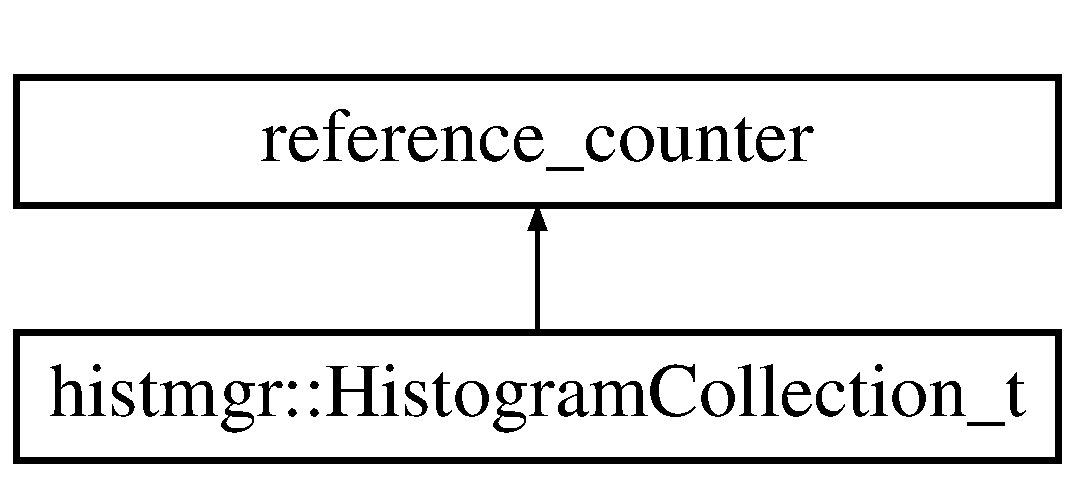
\includegraphics[height=2.000000cm]{classhistmgr_1_1HistogramCollection__t}
\end{center}
\end{figure}
\subsection*{Public Member Functions}
\begin{DoxyCompactItemize}
\item 
{\bf Histogram\-Collection\-\_\-t} (const std\-::string \&collection\-\_\-name, const E\-V\-E\-N\-T\-::\-String\-Vec \&name\-\_\-list, U\-Int\-\_\-t n\-\_\-hist, const {\bf Hist\-Par} \&par) noexcept(false)
\begin{DoxyCompactList}\small\item\em Create a collection of histograms which will have the same binning and the same name (except of a numeric extension). \end{DoxyCompactList}\item 
{\bf Histogram\-Collection\-\_\-t} (const std\-::string \&collection\-\_\-name, const E\-V\-E\-N\-T\-::\-String\-Vec \&name\-\_\-list, const lcio\-::\-Int\-Vec \&n\-\_\-hist\-\_\-list, const {\bf Hist\-Par} \&par)
\begin{DoxyCompactList}\small\item\em Create a collection of histograms which will have the same binning and the same name (except of a numeric extension). \end{DoxyCompactList}\item 
{\bf Histogram\-Collection\-\_\-t} (lcio\-::\-L\-C\-Collection $\ast$histograms, lcio\-::\-Int\-Vec $\ast$indices)
\item 
{\bf Histogram\-Collection\-\_\-t} (lcio\-::\-L\-C\-Collection $\ast$histograms)
\begin{DoxyCompactList}\small\item\em Create a histogram collection from lcio collection. \end{DoxyCompactList}\item 
{\bf Histogram\-Collection\-\_\-t} (const {\bf Histogram\-Collection\-\_\-t} \&a)\label{classhistmgr_1_1HistogramCollection__t_a2021dd1769b2d44df3a2c21fd9cec651}

\begin{DoxyCompactList}\small\item\em copy constructor. \end{DoxyCompactList}\item 
{\bf Histogram\-Collection\-\_\-t} ()\label{classhistmgr_1_1HistogramCollection__t_a707cc7dfca722efaf6c4fd1bd5edaf16}

\begin{DoxyCompactList}\small\item\em Default constructor. \end{DoxyCompactList}\item 
void {\bf delete\-Collection} ()\label{classhistmgr_1_1HistogramCollection__t_aab14375abc9104cae8cd1e244155b95e}

\begin{DoxyCompactList}\small\item\em delete the histogram collection and the index array This method exists instead of a destrctor to prevent copying the arrays (F\-I\-X\-M\-E) \end{DoxyCompactList}\item 
void {\bfseries delete\-Shared\-Storage} ()\label{classhistmgr_1_1HistogramCollection__t_ac9c1e7058781ce12c5409ea6aacea91d}

\item 
lcio\-::\-L\-C\-Collection $\ast$ {\bf create\-Histograms} (const std\-::string \&collection\-\_\-name, const E\-V\-E\-N\-T\-::\-String\-Vec \&name\-\_\-list, U\-Int\-\_\-t n\-\_\-hist, const {\bf Hist\-Par} \&par) noexcept(false)
\begin{DoxyCompactList}\small\item\em create several histograms which will have the same binning and the same name (except of a numeric extension). \end{DoxyCompactList}\item 
lcio\-::\-L\-C\-Collection $\ast$ {\bf create\-Histograms} (const std\-::string \&collection\-\_\-name, const E\-V\-E\-N\-T\-::\-String\-Vec \&name\-\_\-list, const lcio\-::\-Int\-Vec \&n\-\_\-hist\-\_\-list, const {\bf Hist\-Par} \&par) noexcept(false)
\begin{DoxyCompactList}\small\item\em create several histograms which will have the same binning and the same name (except of a numeric extension). \end{DoxyCompactList}\item 
lcio\-::\-L\-C\-Collection $\ast$ {\bf collection} ()
\begin{DoxyCompactList}\small\item\em get the unique group id \end{DoxyCompactList}\item 
const lcio\-::\-L\-C\-Collection $\ast$ {\bf collection} () const 
\begin{DoxyCompactList}\small\item\em get the collection of histograms (read only). \end{DoxyCompactList}\item 
U\-Int\-\_\-t {\bf n} () const \label{classhistmgr_1_1HistogramCollection__t_ac42b746ee1dbd26e5860e92ba1e473ec}

\begin{DoxyCompactList}\small\item\em get the number of histograms in the one dimensional collection. \end{DoxyCompactList}\item 
bool {\bf is2\-D} () const \label{classhistmgr_1_1HistogramCollection__t_a559133040ee3b0194f15c2c957305798}

\begin{DoxyCompactList}\small\item\em Return true if the histogram collection is two instead of one diemensional. \end{DoxyCompactList}\item 
U\-Int\-\_\-t {\bf n\-Major} () const \label{classhistmgr_1_1HistogramCollection__t_a02818178f9b34adc8fc34077f1111ae0}

\begin{DoxyCompactList}\small\item\em get the number of histograms in the one dimensional collection. \end{DoxyCompactList}\item 
U\-Int\-\_\-t {\bf n\-Minor} (U\-Int\-\_\-t major\-\_\-index) const \label{classhistmgr_1_1HistogramCollection__t_aba86c24635ec931b9eef136bddaa897c}

\begin{DoxyCompactList}\small\item\em get the number of histograms in the one dimensional collection. \end{DoxyCompactList}\item 
const {\bf Float\-Histogram1\-D} $\ast$ {\bf histogram} (U\-Int\-\_\-t index) const \label{classhistmgr_1_1HistogramCollection__t_adaa8cee3a607ea20e59a4d3de2e61bea}

\begin{DoxyCompactList}\small\item\em Get one histogram of the collection (read only). \end{DoxyCompactList}\item 
{\bf Float\-Histogram1\-D} $\ast$ {\bf histogram} (U\-Int\-\_\-t index)\label{classhistmgr_1_1HistogramCollection__t_aace80d2015a106ca6d81ac614c58ad23}

\begin{DoxyCompactList}\small\item\em Get one histogram of the collection. \end{DoxyCompactList}\item 
{\bf Float\-Histogram1\-D} $\ast$ {\bf histogram} (U\-Int\-\_\-t major\-\_\-index, U\-Int\-\_\-t minor\-\_\-index)\label{classhistmgr_1_1HistogramCollection__t_abee0821aee3f63a3d3f6f4fc6dc674b7}

\begin{DoxyCompactList}\small\item\em Get one histogram of the collection which is organised as a two dimensional array. \end{DoxyCompactList}\item 
const {\bf Float\-Histogram1\-D} $\ast$ {\bf histogram} (U\-Int\-\_\-t major\-\_\-index, U\-Int\-\_\-t minor\-\_\-index) const \label{classhistmgr_1_1HistogramCollection__t_a64edb699f808ea5628d75bf996ebc70e}

\begin{DoxyCompactList}\small\item\em Get one histogram of the collection which is organised as a two dimensional array (read only). \end{DoxyCompactList}\item 
const std\-::string \& {\bf get\-Name} (U\-Int\-\_\-t major\-\_\-index) const 
\begin{DoxyCompactList}\small\item\em Get the name of the specified element of the histogram collection. \end{DoxyCompactList}\end{DoxyCompactItemize}
\subsection*{Static Protected Attributes}
\begin{DoxyCompactItemize}
\item 
static const std\-::string {\bfseries \-\_\-\-\_\-histogram\-Name\-Parameter\-Name}\label{classhistmgr_1_1HistogramCollection__t_a2c356864c2b153d6efb4758d025196cd}

\end{DoxyCompactItemize}
\subsection*{Private Member Functions}
\begin{DoxyCompactItemize}
\item 
void {\bf copy\-Names} () const 
\begin{DoxyCompactList}\small\item\em Copy the names from the collection to an accessible vector. \end{DoxyCompactList}\end{DoxyCompactItemize}
\subsection*{Private Attributes}
\begin{DoxyCompactItemize}
\item 
lcio\-::\-L\-C\-Collection $\ast$ {\bf \-\_\-histogram\-Col}\label{classhistmgr_1_1HistogramCollection__t_a2336156a2439b0ee1f45e0328b685186}

\begin{DoxyCompactList}\small\item\em the histogram collection \end{DoxyCompactList}\item 
lcio\-::\-Int\-Vec $\ast$ {\bf \-\_\-major\-Index}
\begin{DoxyCompactList}\small\item\em optional list of offset to form a two dimensional array out of the list. \end{DoxyCompactList}\item 
lcio\-::\-String\-Vec {\bf \-\_\-name\-List}
\begin{DoxyCompactList}\small\item\em A vector which contains one name for all histograms of the collection or a name for each element. \end{DoxyCompactList}\end{DoxyCompactItemize}
\subsection*{Static Private Attributes}
\begin{DoxyCompactItemize}
\item 
static const std\-::string {\bfseries \-\_\-\-\_\-major\-Index\-Parameter\-Name}\label{classhistmgr_1_1HistogramCollection__t_a994eb5d3bbbd406c9713cc8f48a0c579}

\item 
static const std\-::string {\bfseries \-\_\-\-\_\-default\-Histogram\-Name}\label{classhistmgr_1_1HistogramCollection__t_a2185171919e2ed84ae60cbd106f8388f}

\end{DoxyCompactItemize}
\subsection*{Friends}
\begin{DoxyCompactItemize}
\item 
class {\bfseries Hist\-Mgr}\label{classhistmgr_1_1HistogramCollection__t_a3cc85db784d7651390e41024125eb3a0}

\end{DoxyCompactItemize}
\subsection*{Additional Inherited Members}


\subsection{Detailed Description}
One or two dimensional collection of histograms. 

Definition at line 16 of file Histogram\-Collection\-\_\-t.\-hh.



\subsection{Constructor \& Destructor Documentation}
\index{histmgr\-::\-Histogram\-Collection\-\_\-t@{histmgr\-::\-Histogram\-Collection\-\_\-t}!Histogram\-Collection\-\_\-t@{Histogram\-Collection\-\_\-t}}
\index{Histogram\-Collection\-\_\-t@{Histogram\-Collection\-\_\-t}!histmgr::HistogramCollection_t@{histmgr\-::\-Histogram\-Collection\-\_\-t}}
\subsubsection[{Histogram\-Collection\-\_\-t}]{\setlength{\rightskip}{0pt plus 5cm}histmgr\-::\-Histogram\-Collection\-\_\-t\-::\-Histogram\-Collection\-\_\-t (
\begin{DoxyParamCaption}
\item[{const std\-::string \&}]{collection\-\_\-name, }
\item[{const E\-V\-E\-N\-T\-::\-String\-Vec \&}]{name\-\_\-list, }
\item[{U\-Int\-\_\-t}]{n\-\_\-hist, }
\item[{const {\bf Hist\-Par} \&}]{par}
\end{DoxyParamCaption}
)\hspace{0.3cm}{\ttfamily [inline]}, {\ttfamily [noexcept]}}\label{classhistmgr_1_1HistogramCollection__t_a7cdb089b826e743c88d8ba6010eda963}


Create a collection of histograms which will have the same binning and the same name (except of a numeric extension). 


\begin{DoxyParams}{Parameters}
{\em collection\-\_\-name} & the of the histogram collection \\
\hline
{\em name\-\_\-list} & a vector containing the names of the histograms whose length is either equals n\-\_\-hist or is zero. In the latter case the collection name is used for the all histograms. \\
\hline
{\em n\-\_\-hist} & the number of histograms to be created \\
\hline
{\em par} & the binning of the histograms\\
\hline
\end{DoxyParams}
The histograms are only written to a file if the histogram group, to which this histogram belongs, is assigned to a file (\doxyref{histmgr\-::\-Hist\-Mgr\-::assign\-File\-Name}{p.}{classhistmgr_1_1HistMgr_a20e3c96a8ba6175c8036918ca7acb1e2}). 

Definition at line 32 of file Histogram\-Collection\-\_\-t.\-hh.



References create\-Histograms().

\index{histmgr\-::\-Histogram\-Collection\-\_\-t@{histmgr\-::\-Histogram\-Collection\-\_\-t}!Histogram\-Collection\-\_\-t@{Histogram\-Collection\-\_\-t}}
\index{Histogram\-Collection\-\_\-t@{Histogram\-Collection\-\_\-t}!histmgr::HistogramCollection_t@{histmgr\-::\-Histogram\-Collection\-\_\-t}}
\subsubsection[{Histogram\-Collection\-\_\-t}]{\setlength{\rightskip}{0pt plus 5cm}histmgr\-::\-Histogram\-Collection\-\_\-t\-::\-Histogram\-Collection\-\_\-t (
\begin{DoxyParamCaption}
\item[{const std\-::string \&}]{collection\-\_\-name, }
\item[{const E\-V\-E\-N\-T\-::\-String\-Vec \&}]{name\-\_\-list, }
\item[{const lcio\-::\-Int\-Vec \&}]{n\-\_\-hist\-\_\-list, }
\item[{const {\bf Hist\-Par} \&}]{par}
\end{DoxyParamCaption}
)\hspace{0.3cm}{\ttfamily [inline]}}\label{classhistmgr_1_1HistogramCollection__t_acaca47dfbc11a7ca511a084efdfe8737}


Create a collection of histograms which will have the same binning and the same name (except of a numeric extension). 


\begin{DoxyParams}{Parameters}
{\em collection\-\_\-name} & the of the histogram collection \\
\hline
{\em name\-\_\-list} & a vector containing the names of the histograms whose length is either equals n\-\_\-hist or is zero. In the latter case the collection name is used for the all histograms. \\
\hline
{\em n\-\_\-hist\-\_\-list} & the number of histograms to be created \\
\hline
{\em par} & the binning of the histogram\\
\hline
\end{DoxyParams}
\begin{DoxyReturn}{Returns}
pointer to the histogram collection
\end{DoxyReturn}
The histograms are only written to a file if the histogram group, to which this histogram belongs, is assigned to a file (\doxyref{histmgr\-::\-Hist\-Mgr\-::assign\-File\-Name}{p.}{classhistmgr_1_1HistMgr_a20e3c96a8ba6175c8036918ca7acb1e2}). 

Definition at line 57 of file Histogram\-Collection\-\_\-t.\-hh.



References create\-Histograms().

\index{histmgr\-::\-Histogram\-Collection\-\_\-t@{histmgr\-::\-Histogram\-Collection\-\_\-t}!Histogram\-Collection\-\_\-t@{Histogram\-Collection\-\_\-t}}
\index{Histogram\-Collection\-\_\-t@{Histogram\-Collection\-\_\-t}!histmgr::HistogramCollection_t@{histmgr\-::\-Histogram\-Collection\-\_\-t}}
\subsubsection[{Histogram\-Collection\-\_\-t}]{\setlength{\rightskip}{0pt plus 5cm}histmgr\-::\-Histogram\-Collection\-\_\-t\-::\-Histogram\-Collection\-\_\-t (
\begin{DoxyParamCaption}
\item[{lcio\-::\-L\-C\-Collection $\ast$}]{histograms, }
\item[{lcio\-::\-Int\-Vec $\ast$}]{indices}
\end{DoxyParamCaption}
)\hspace{0.3cm}{\ttfamily [inline]}}\label{classhistmgr_1_1HistogramCollection__t_aa97ddab34cc197f39f0af48891adaaa4}

\begin{DoxyParams}{Parameters}
{\em histograms} & the linearised one or two dimensional collection of histograms \\
\hline
{\em indices} & optional list of indicies used to give two dimensional access to the histogram list. for each possible index of the first dimension is needed which contains the offset in the list. The second index is added to this offset. \\
\hline
\end{DoxyParams}


Definition at line 74 of file Histogram\-Collection\-\_\-t.\-hh.



References \-\_\-major\-Index.

\index{histmgr\-::\-Histogram\-Collection\-\_\-t@{histmgr\-::\-Histogram\-Collection\-\_\-t}!Histogram\-Collection\-\_\-t@{Histogram\-Collection\-\_\-t}}
\index{Histogram\-Collection\-\_\-t@{Histogram\-Collection\-\_\-t}!histmgr::HistogramCollection_t@{histmgr\-::\-Histogram\-Collection\-\_\-t}}
\subsubsection[{Histogram\-Collection\-\_\-t}]{\setlength{\rightskip}{0pt plus 5cm}histmgr\-::\-Histogram\-Collection\-\_\-t\-::\-Histogram\-Collection\-\_\-t (
\begin{DoxyParamCaption}
\item[{lcio\-::\-L\-C\-Collection $\ast$}]{histograms}
\end{DoxyParamCaption}
)\hspace{0.3cm}{\ttfamily [inline]}}\label{classhistmgr_1_1HistogramCollection__t_a4699957d2f2d7fb40949572ea311affd}


Create a histogram collection from lcio collection. 


\begin{DoxyParams}{Parameters}
{\em histograms} & the linearised one or two dimensional collection of histograms (two dimensional collections have the collection parameter \char`\"{}major\char`\"{}). The method does not verify whether the lcio collection really is a histogram collection. However, if the collection has the parameter \char`\"{}major\char`\"{} it creates an index vector (costly operation) assuming that it is a 2d array instead of a 1d array(i.\-e. collection). The unique group id remains undedfined since it is not stored in the lcio collection. \\
\hline
\end{DoxyParams}


Definition at line 98 of file Histogram\-Collection\-\_\-t.\-hh.



References \-\_\-major\-Index.



\subsection{Member Function Documentation}
\index{histmgr\-::\-Histogram\-Collection\-\_\-t@{histmgr\-::\-Histogram\-Collection\-\_\-t}!collection@{collection}}
\index{collection@{collection}!histmgr::HistogramCollection_t@{histmgr\-::\-Histogram\-Collection\-\_\-t}}
\subsubsection[{collection}]{\setlength{\rightskip}{0pt plus 5cm}lcio\-::\-L\-C\-Collection$\ast$ histmgr\-::\-Histogram\-Collection\-\_\-t\-::collection (
\begin{DoxyParamCaption}
{}
\end{DoxyParamCaption}
)\hspace{0.3cm}{\ttfamily [inline]}}\label{classhistmgr_1_1HistogramCollection__t_a9b7d3e45deaea4d7e531b7e82f2cf033}


get the unique group id 

get the collection of histograms. The index array needed for the two dimensional acces is added as a parameter named \char`\"{}major\char`\"{}. 

Definition at line 198 of file Histogram\-Collection\-\_\-t.\-hh.



References \-\_\-histogram\-Col.

\index{histmgr\-::\-Histogram\-Collection\-\_\-t@{histmgr\-::\-Histogram\-Collection\-\_\-t}!collection@{collection}}
\index{collection@{collection}!histmgr::HistogramCollection_t@{histmgr\-::\-Histogram\-Collection\-\_\-t}}
\subsubsection[{collection}]{\setlength{\rightskip}{0pt plus 5cm}const lcio\-::\-L\-C\-Collection$\ast$ histmgr\-::\-Histogram\-Collection\-\_\-t\-::collection (
\begin{DoxyParamCaption}
{}
\end{DoxyParamCaption}
) const\hspace{0.3cm}{\ttfamily [inline]}}\label{classhistmgr_1_1HistogramCollection__t_a9899c0767792c848c3b075c5a38ecc0a}


get the collection of histograms (read only). 

The index array needed for the two dimensional acces is added as a parameter named \char`\"{}major\char`\"{}. 

Definition at line 203 of file Histogram\-Collection\-\_\-t.\-hh.



References \-\_\-histogram\-Col.

\index{histmgr\-::\-Histogram\-Collection\-\_\-t@{histmgr\-::\-Histogram\-Collection\-\_\-t}!copy\-Names@{copy\-Names}}
\index{copy\-Names@{copy\-Names}!histmgr::HistogramCollection_t@{histmgr\-::\-Histogram\-Collection\-\_\-t}}
\subsubsection[{copy\-Names}]{\setlength{\rightskip}{0pt plus 5cm}void histmgr\-::\-Histogram\-Collection\-\_\-t\-::copy\-Names (
\begin{DoxyParamCaption}
{}
\end{DoxyParamCaption}
) const\hspace{0.3cm}{\ttfamily [inline]}, {\ttfamily [private]}}\label{classhistmgr_1_1HistogramCollection__t_a0af499d244db5de042c76f98e664f8fe}


Copy the names from the collection to an accessible vector. 

The vector of histogram names is attached as a parameter to the L\-C\-Collection. 

Definition at line 351 of file Histogram\-Collection\-\_\-t.\-hh.



References \-\_\-histogram\-Col, and \-\_\-name\-List.



Referenced by get\-Name().

\index{histmgr\-::\-Histogram\-Collection\-\_\-t@{histmgr\-::\-Histogram\-Collection\-\_\-t}!create\-Histograms@{create\-Histograms}}
\index{create\-Histograms@{create\-Histograms}!histmgr::HistogramCollection_t@{histmgr\-::\-Histogram\-Collection\-\_\-t}}
\subsubsection[{create\-Histograms}]{\setlength{\rightskip}{0pt plus 5cm}lcio\-::\-L\-C\-Collection $\ast$ histmgr\-::\-Histogram\-Collection\-\_\-t\-::create\-Histograms (
\begin{DoxyParamCaption}
\item[{const std\-::string \&}]{collection\-\_\-name, }
\item[{const E\-V\-E\-N\-T\-::\-String\-Vec \&}]{name\-\_\-list, }
\item[{U\-Int\-\_\-t}]{n\-\_\-hist, }
\item[{const {\bf Hist\-Par} \&}]{par}
\end{DoxyParamCaption}
)\hspace{0.3cm}{\ttfamily [noexcept]}}\label{classhistmgr_1_1HistogramCollection__t_a0eaf6ae908e2c9f742f2c7af2cfc8f03}


create several histograms which will have the same binning and the same name (except of a numeric extension). 


\begin{DoxyParams}{Parameters}
{\em collection\-\_\-name} & the of the histogram collection \\
\hline
{\em name\-\_\-list} & a vector containing the names of the histograms whose length is either equals n\-\_\-hist or is zero. In the latter case the collection name is used for the all histograms. \\
\hline
{\em n\-\_\-hist} & the number of histograms to be created \\
\hline
{\em par} & the binning of the histograms\\
\hline
\end{DoxyParams}
\begin{DoxyReturn}{Returns}
pointer to the histogram collection.
\end{DoxyReturn}
The histograms are only written to a file if the histogram group, to which this histogram belongs, is assigned to a file (\doxyref{histmgr\-::\-Hist\-Mgr\-::assign\-File\-Name}{p.}{classhistmgr_1_1HistMgr_a20e3c96a8ba6175c8036918ca7acb1e2}). 

Definition at line 16 of file Histogram\-Collection\-\_\-t.\-cc.



Referenced by Histogram\-Collection\-\_\-t().

\index{histmgr\-::\-Histogram\-Collection\-\_\-t@{histmgr\-::\-Histogram\-Collection\-\_\-t}!create\-Histograms@{create\-Histograms}}
\index{create\-Histograms@{create\-Histograms}!histmgr::HistogramCollection_t@{histmgr\-::\-Histogram\-Collection\-\_\-t}}
\subsubsection[{create\-Histograms}]{\setlength{\rightskip}{0pt plus 5cm}lcio\-::\-L\-C\-Collection $\ast$ histmgr\-::\-Histogram\-Collection\-\_\-t\-::create\-Histograms (
\begin{DoxyParamCaption}
\item[{const std\-::string \&}]{collection\-\_\-name, }
\item[{const E\-V\-E\-N\-T\-::\-String\-Vec \&}]{name\-\_\-list, }
\item[{const lcio\-::\-Int\-Vec \&}]{n\-\_\-hist\-\_\-list, }
\item[{const {\bf Hist\-Par} \&}]{par}
\end{DoxyParamCaption}
)\hspace{0.3cm}{\ttfamily [noexcept]}}\label{classhistmgr_1_1HistogramCollection__t_a7d061571d8615249ad3c7b24331a3f76}


create several histograms which will have the same binning and the same name (except of a numeric extension). 


\begin{DoxyParams}{Parameters}
{\em collection\-\_\-name} & the of the histogram collection \\
\hline
{\em name\-\_\-list} & a vector containing the names of the histograms whose length is either equals n\-\_\-hist or is zero. In the latter case the collection name is used for the all histograms. \\
\hline
{\em n\-\_\-hist\-\_\-list} & the number of histograms to be created \\
\hline
{\em par} & the binning of the histogram\\
\hline
\end{DoxyParams}
\begin{DoxyReturn}{Returns}
pointer to the histogram collection
\end{DoxyReturn}
The histograms are only written to a file if the histogram group, to which this histogram belongs, is assigned to a file (\doxyref{histmgr\-::\-Hist\-Mgr\-::assign\-File\-Name}{p.}{classhistmgr_1_1HistMgr_a20e3c96a8ba6175c8036918ca7acb1e2}). 

Definition at line 66 of file Histogram\-Collection\-\_\-t.\-cc.

\index{histmgr\-::\-Histogram\-Collection\-\_\-t@{histmgr\-::\-Histogram\-Collection\-\_\-t}!get\-Name@{get\-Name}}
\index{get\-Name@{get\-Name}!histmgr::HistogramCollection_t@{histmgr\-::\-Histogram\-Collection\-\_\-t}}
\subsubsection[{get\-Name}]{\setlength{\rightskip}{0pt plus 5cm}const std\-::string\& histmgr\-::\-Histogram\-Collection\-\_\-t\-::get\-Name (
\begin{DoxyParamCaption}
\item[{U\-Int\-\_\-t}]{major\-\_\-index}
\end{DoxyParamCaption}
) const\hspace{0.3cm}{\ttfamily [inline]}}\label{classhistmgr_1_1HistogramCollection__t_a5fdddf211d50bd490d736c42b953de90}


Get the name of the specified element of the histogram collection. 


\begin{DoxyParams}{Parameters}
{\em major\-\_\-index} & the index of the histogram element or in case of an 2\-D histogram array the major index. \\
\hline
\end{DoxyParams}
\begin{DoxyReturn}{Returns}
a reference to the name. 
\end{DoxyReturn}


Definition at line 321 of file Histogram\-Collection\-\_\-t.\-hh.



References \-\_\-name\-List, and copy\-Names().



\subsection{Field Documentation}
\index{histmgr\-::\-Histogram\-Collection\-\_\-t@{histmgr\-::\-Histogram\-Collection\-\_\-t}!\-\_\-major\-Index@{\-\_\-major\-Index}}
\index{\-\_\-major\-Index@{\-\_\-major\-Index}!histmgr::HistogramCollection_t@{histmgr\-::\-Histogram\-Collection\-\_\-t}}
\subsubsection[{\-\_\-major\-Index}]{\setlength{\rightskip}{0pt plus 5cm}lcio\-::\-Int\-Vec$\ast$ histmgr\-::\-Histogram\-Collection\-\_\-t\-::\-\_\-major\-Index\hspace{0.3cm}{\ttfamily [private]}}\label{classhistmgr_1_1HistogramCollection__t_aab803b274bb05413461efac60406e701}


optional list of offset to form a two dimensional array out of the list. 



Definition at line 362 of file Histogram\-Collection\-\_\-t.\-hh.



Referenced by delete\-Collection(), histogram(), Histogram\-Collection\-\_\-t(), is2\-D(), n\-Major(), and n\-Minor().

\index{histmgr\-::\-Histogram\-Collection\-\_\-t@{histmgr\-::\-Histogram\-Collection\-\_\-t}!\-\_\-name\-List@{\-\_\-name\-List}}
\index{\-\_\-name\-List@{\-\_\-name\-List}!histmgr::HistogramCollection_t@{histmgr\-::\-Histogram\-Collection\-\_\-t}}
\subsubsection[{\-\_\-name\-List}]{\setlength{\rightskip}{0pt plus 5cm}lcio\-::\-String\-Vec histmgr\-::\-Histogram\-Collection\-\_\-t\-::\-\_\-name\-List\hspace{0.3cm}{\ttfamily [mutable]}, {\ttfamily [private]}}\label{classhistmgr_1_1HistogramCollection__t_ab9ed53cc2ab98fc16123a22e3b1d0f2c}


A vector which contains one name for all histograms of the collection or a name for each element. 



Definition at line 364 of file Histogram\-Collection\-\_\-t.\-hh.



Referenced by copy\-Names(), and get\-Name().



The documentation for this class was generated from the following files\-:\begin{DoxyCompactItemize}
\item 
Histogram\-Collection\-\_\-t.\-hh\item 
Histogram\-Collection\-\_\-t.\-cc\end{DoxyCompactItemize}

\section{histmgr\-:\-:Hist\-Mgr\-:\-:Histogram\-Group\-Data\-\_\-t Class Reference}
\label{classhistmgr_1_1HistMgr_1_1HistogramGroupData__t}\index{histmgr\-::\-Hist\-Mgr\-::\-Histogram\-Group\-Data\-\_\-t@{histmgr\-::\-Hist\-Mgr\-::\-Histogram\-Group\-Data\-\_\-t}}


id, destination file and folder of a histogram group  




{\ttfamily \#include $<$Hist\-Mgr.\-hh$>$}

\subsection*{Public Member Functions}
\begin{DoxyCompactItemize}
\item 
{\bfseries Histogram\-Group\-Data\-\_\-t} (std\-::string file\-\_\-name, std\-::string folder\-\_\-name)\label{classhistmgr_1_1HistMgr_1_1HistogramGroupData__t_a07a5f211a1b240c9834f69c67b4f6203}

\item 
U\-Int\-\_\-t {\bfseries id} () const \label{classhistmgr_1_1HistMgr_1_1HistogramGroupData__t_a30189a30c3e48bf0f70779642a4e0b6d}

\item 
U\-Int\-\_\-t {\bfseries version} () const \label{classhistmgr_1_1HistMgr_1_1HistogramGroupData__t_a53a43a01a611eeb58986d06cf112baaf}

\item 
void {\bfseries increment\-Version} ()\label{classhistmgr_1_1HistMgr_1_1HistogramGroupData__t_a523ffb8dee6ceb8c802d7582d65d8a0f}

\item 
const std\-::string \& {\bfseries file\-Name} () const \label{classhistmgr_1_1HistMgr_1_1HistogramGroupData__t_acd20c1c6b5e1204649f0d7603b0f6ee2}

\item 
const std\-::string \& {\bfseries folder\-Name} () const \label{classhistmgr_1_1HistMgr_1_1HistogramGroupData__t_a886cab942d93e6ba0485ed6eb82afd02}

\item 
{\bf Histogram\-Group\-Data\-\_\-t} \& {\bfseries set\-File\-Name} (const std\-::string \&file\-\_\-name)\label{classhistmgr_1_1HistMgr_1_1HistogramGroupData__t_a4d9c6b374964d3def4ac44f60596143d}

\item 
{\bf Histogram\-Group\-Data\-\_\-t} \& {\bfseries set\-Folder\-Name} (const std\-::string \&folder\-\_\-name)\label{classhistmgr_1_1HistMgr_1_1HistogramGroupData__t_a74225cdfb078be31da16dfe9482d62bc}

\item 
void {\bfseries ref} ()\label{classhistmgr_1_1HistMgr_1_1HistogramGroupData__t_a4bc6ddd417970ce1c00d53781b093bb4}

\item 
void {\bfseries unref} ()\label{classhistmgr_1_1HistMgr_1_1HistogramGroupData__t_ab8019cd94a1bdebebb805ddb5d972500}

\item 
U\-Int\-\_\-t {\bfseries references} () const \label{classhistmgr_1_1HistMgr_1_1HistogramGroupData__t_ab3e91d6c35a226699da929e9141fd2a9}

\item 
bool {\bfseries is\-Referenced} () const \label{classhistmgr_1_1HistMgr_1_1HistogramGroupData__t_abedbf506b91a7609e9a9b78a2039a26b}

\end{DoxyCompactItemize}
\subsection*{Protected Member Functions}
\begin{DoxyCompactItemize}
\item 
void {\bfseries set\-Id} (unsigned int id)\label{classhistmgr_1_1HistMgr_1_1HistogramGroupData__t_a4b84f56cb6cff0f0d3fbcdd5213be5db}

\end{DoxyCompactItemize}
\subsection*{Protected Attributes}
\begin{DoxyCompactItemize}
\item 
U\-Int\-\_\-t {\bf \-\_\-ref\-Counter}\label{classhistmgr_1_1HistMgr_1_1HistogramGroupData__t_a9e13ffec297c7682e7846f3fc96a4904}

\begin{DoxyCompactList}\small\item\em number of users of this group \end{DoxyCompactList}\item 
U\-Int\-\_\-t {\bf \-\_\-id}\label{classhistmgr_1_1HistMgr_1_1HistogramGroupData__t_a2aa126884bac9c85f0063466bcc44d47}

\begin{DoxyCompactList}\small\item\em unique histogram group id \end{DoxyCompactList}\item 
std\-::string {\bf \-\_\-file\-Name}\label{classhistmgr_1_1HistMgr_1_1HistogramGroupData__t_a887041e492c5179f576e2ff0348286e0}

\begin{DoxyCompactList}\small\item\em file to which all the histograms of this group will be written \end{DoxyCompactList}\item 
std\-::string {\bf \-\_\-folder\-Name}\label{classhistmgr_1_1HistMgr_1_1HistogramGroupData__t_a1a2b8f1b779a7d2f62da302d4d77b620}

\begin{DoxyCompactList}\small\item\em folder inside the file to which all the histograms of this group will be written \end{DoxyCompactList}\item 
U\-Int\-\_\-t {\bfseries \-\_\-version}\label{classhistmgr_1_1HistMgr_1_1HistogramGroupData__t_a14fe90666c845803d60b98ac8d15db85}

\end{DoxyCompactItemize}
\subsection*{Friends}
\begin{DoxyCompactItemize}
\item 
class {\bfseries Hist\-Mgr}\label{classhistmgr_1_1HistMgr_1_1HistogramGroupData__t_a3cc85db784d7651390e41024125eb3a0}

\end{DoxyCompactItemize}


\subsection{Detailed Description}
id, destination file and folder of a histogram group 

\begin{DoxyRefDesc}{Todo}
\item[{\bf Todo}]remove \-\_\-id \end{DoxyRefDesc}


Definition at line 50 of file Hist\-Mgr.\-hh.



The documentation for this class was generated from the following file\-:\begin{DoxyCompactItemize}
\item 
Hist\-Mgr.\-hh\end{DoxyCompactItemize}

\section{histmgr\-:\-:Histogram\-Output Class Reference}
\label{classhistmgr_1_1HistogramOutput}\index{histmgr\-::\-Histogram\-Output@{histmgr\-::\-Histogram\-Output}}


Processor which writes histogram groups to files at the end of the processing.  




{\ttfamily \#include $<$Histogram\-Output.\-hh$>$}

Inheritance diagram for histmgr\-:\-:Histogram\-Output\-:\begin{figure}[H]
\begin{center}
\leavevmode
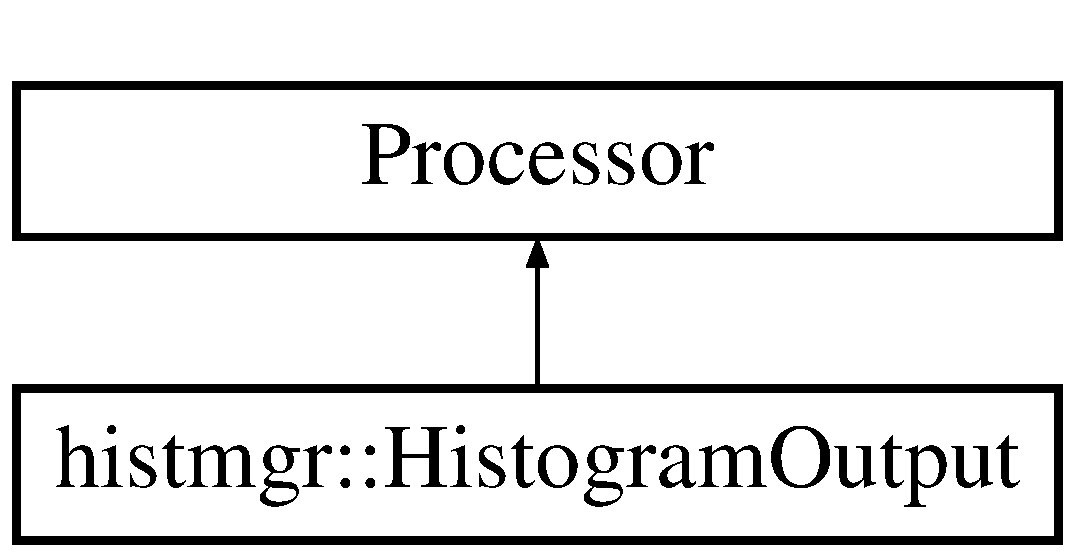
\includegraphics[height=2.000000cm]{classhistmgr_1_1HistogramOutput}
\end{center}
\end{figure}
\subsection*{Public Member Functions}
\begin{DoxyCompactItemize}
\item 
Processor $\ast$ {\bfseries new\-Processor} ()\label{classhistmgr_1_1HistogramOutput_aec1ae9dabcace0c5d9c425d4305153aa}

\item 
void {\bf init} ()
\begin{DoxyCompactList}\small\item\em Called at the begin of the job before anything is read. \end{DoxyCompactList}\item 
void {\bf end} ()
\begin{DoxyCompactList}\small\item\em Called for every run, e.\-g. \end{DoxyCompactList}\end{DoxyCompactItemize}
\subsection*{Protected Attributes}
\begin{DoxyCompactItemize}
\item 
String\-Vec {\bfseries \-\_\-file\-Folder\-Assignment}\label{classhistmgr_1_1HistogramOutput_acf932812a8468eb3106dca6a5b9040ea}

\end{DoxyCompactItemize}


\subsection{Detailed Description}
Processor which writes histogram groups to files at the end of the processing. 

The histogram groups and their destination files are specified by marlin processor parameters. Each histogram group can be written to a seperate file. 

Definition at line 22 of file Histogram\-Output.\-hh.



\subsection{Member Function Documentation}
\index{histmgr\-::\-Histogram\-Output@{histmgr\-::\-Histogram\-Output}!end@{end}}
\index{end@{end}!histmgr::HistogramOutput@{histmgr\-::\-Histogram\-Output}}
\subsubsection[{end}]{\setlength{\rightskip}{0pt plus 5cm}void histmgr\-::\-Histogram\-Output\-::end (
\begin{DoxyParamCaption}
{}
\end{DoxyParamCaption}
)}\label{classhistmgr_1_1HistogramOutput_ae9d8650a0e3d0608fa1fa86849ab48ad}


Called for every run, e.\-g. 

overwrite to initialize run dependent histograms.\-Called for every event -\/ the working horse. 

Definition at line 117 of file Histogram\-Output.\-cc.



References histmgr\-::\-Hist\-Mgr\-::write\-Histograms().

\index{histmgr\-::\-Histogram\-Output@{histmgr\-::\-Histogram\-Output}!init@{init}}
\index{init@{init}!histmgr::HistogramOutput@{histmgr\-::\-Histogram\-Output}}
\subsubsection[{init}]{\setlength{\rightskip}{0pt plus 5cm}void histmgr\-::\-Histogram\-Output\-::init (
\begin{DoxyParamCaption}
{}
\end{DoxyParamCaption}
)}\label{classhistmgr_1_1HistogramOutput_a191f76c80a79ad920e2e209426e7c2fe}


Called at the begin of the job before anything is read. 

Use to initialize the processor, e.\-g. book histograms. 

Definition at line 57 of file Histogram\-Output.\-cc.



References histmgr\-::\-Hist\-Mgr\-::assign\-File\-Name(), and histmgr\-::\-Hist\-Mgr\-::warn\-On\-Unassigned().



The documentation for this class was generated from the following files\-:\begin{DoxyCompactItemize}
\item 
Histogram\-Output.\-hh\item 
Histogram\-Output.\-cc\end{DoxyCompactItemize}

\section{Hist\-Par Class Reference}
\label{classHistPar}\index{Hist\-Par@{Hist\-Par}}


Class to describe the binning of equidistant histograms.  




{\ttfamily \#include $<$Hist\-Par.\-hh$>$}

\subsection*{Public Member Functions}
\begin{DoxyCompactItemize}
\item 
{\bf Hist\-Par} ()
\begin{DoxyCompactList}\small\item\em Default constructor. \end{DoxyCompactList}\item 
{\bf Hist\-Par} (U\-Int\-\_\-t n\-\_\-bins, Float\-\_\-t x\-\_\-min, Float\-\_\-t x\-\_\-max)
\begin{DoxyCompactList}\small\item\em Constructor. \end{DoxyCompactList}\item 
{\bf Hist\-Par} \& {\bf set\-N\-Bins} (U\-Int\-\_\-t n\-\_\-bins)
\begin{DoxyCompactList}\small\item\em Set the number of bins. \end{DoxyCompactList}\item 
{\bf Hist\-Par} \& {\bf set\-X\-Min} (Float\-\_\-t x\-\_\-min)
\begin{DoxyCompactList}\small\item\em Set the lower edge of the first bin. \end{DoxyCompactList}\item 
{\bf Hist\-Par} \& {\bf set\-X\-Max} (Float\-\_\-t x\-\_\-max)
\begin{DoxyCompactList}\small\item\em set the upper edge of the last bin. \end{DoxyCompactList}\item 
U\-Int\-\_\-t {\bf n\-Bins} () const 
\begin{DoxyCompactList}\small\item\em The number of bins to be used. \end{DoxyCompactList}\item 
Float\-\_\-t {\bf x\-Min} () const 
\begin{DoxyCompactList}\small\item\em The lower edge of the first bin. \end{DoxyCompactList}\item 
Float\-\_\-t {\bf x\-Max} () const 
\begin{DoxyCompactList}\small\item\em The upper edge of the last bin. \end{DoxyCompactList}\end{DoxyCompactItemize}
\subsection*{Protected Attributes}
\begin{DoxyCompactItemize}
\item 
U\-Int\-\_\-t {\bfseries \-\_\-n\-Bins}\label{classHistPar_a2f92256cb42728ba7451833957f8e736}

\item 
Float\-\_\-t {\bfseries \-\_\-x\-Min}\label{classHistPar_a42e200659eadda3a8cc9d437b508fd69}

\item 
Float\-\_\-t {\bfseries \-\_\-x\-Max}\label{classHistPar_a231c21049680a88f30390d2c8e2b24f1}

\end{DoxyCompactItemize}


\subsection{Detailed Description}
Class to describe the binning of equidistant histograms. 

Definition at line 8 of file Hist\-Par.\-hh.



\subsection{Constructor \& Destructor Documentation}
\index{Hist\-Par@{Hist\-Par}!Hist\-Par@{Hist\-Par}}
\index{Hist\-Par@{Hist\-Par}!HistPar@{Hist\-Par}}
\subsubsection[{Hist\-Par}]{\setlength{\rightskip}{0pt plus 5cm}Hist\-Par\-::\-Hist\-Par (
\begin{DoxyParamCaption}
{}
\end{DoxyParamCaption}
)\hspace{0.3cm}{\ttfamily [inline]}}\label{classHistPar_a03ca9e6513517a8d0748eeb9b3723366}


Default constructor. 

The binning defined by the default constructor is invalid. 

Definition at line 14 of file Hist\-Par.\-hh.

\index{Hist\-Par@{Hist\-Par}!Hist\-Par@{Hist\-Par}}
\index{Hist\-Par@{Hist\-Par}!HistPar@{Hist\-Par}}
\subsubsection[{Hist\-Par}]{\setlength{\rightskip}{0pt plus 5cm}Hist\-Par\-::\-Hist\-Par (
\begin{DoxyParamCaption}
\item[{U\-Int\-\_\-t}]{n\-\_\-bins, }
\item[{Float\-\_\-t}]{x\-\_\-min, }
\item[{Float\-\_\-t}]{x\-\_\-max}
\end{DoxyParamCaption}
)\hspace{0.3cm}{\ttfamily [inline]}}\label{classHistPar_aa2be58b98431631d7dd39cc214a88c62}


Constructor. 

\begin{DoxySeeAlso}{See Also}
\doxyref{set\-N\-Bins}{p.}{classHistPar_a56c5bd27973aadd8f2f0d2b35e9fb783},\doxyref{set\-X\-Min}{p.}{classHistPar_ae822c2e2fdc618936d86b7fb0c6ba6fe},set\-Xmax 
\end{DoxySeeAlso}


Definition at line 19 of file Hist\-Par.\-hh.



\subsection{Member Function Documentation}
\index{Hist\-Par@{Hist\-Par}!n\-Bins@{n\-Bins}}
\index{n\-Bins@{n\-Bins}!HistPar@{Hist\-Par}}
\subsubsection[{n\-Bins}]{\setlength{\rightskip}{0pt plus 5cm}U\-Int\-\_\-t Hist\-Par\-::n\-Bins (
\begin{DoxyParamCaption}
{}
\end{DoxyParamCaption}
) const\hspace{0.3cm}{\ttfamily [inline]}}\label{classHistPar_a6d6a4c67550ec02a8e0233b89897baf8}


The number of bins to be used. 

This does not include overflow and underflow bins. Thus, generally two more bins will be used to store the overflow and the underflow. 

Definition at line 41 of file Hist\-Par.\-hh.



Referenced by histmgr\-::\-Float\-Histogram1\-D\-::\-Float\-Histogram1\-D(), histmgr\-::\-Float\-Histogram2\-D\-::\-Float\-Histogram2\-D(), histmgr\-::\-Profile1\-D\-::\-Profile1\-D(), and histmgr\-::\-Histogram1\-D\-::set\-Binning().

\index{Hist\-Par@{Hist\-Par}!set\-N\-Bins@{set\-N\-Bins}}
\index{set\-N\-Bins@{set\-N\-Bins}!HistPar@{Hist\-Par}}
\subsubsection[{set\-N\-Bins}]{\setlength{\rightskip}{0pt plus 5cm}{\bf Hist\-Par}\& Hist\-Par\-::set\-N\-Bins (
\begin{DoxyParamCaption}
\item[{U\-Int\-\_\-t}]{n\-\_\-bins}
\end{DoxyParamCaption}
)\hspace{0.3cm}{\ttfamily [inline]}}\label{classHistPar_a56c5bd27973aadd8f2f0d2b35e9fb783}


Set the number of bins. 

This does not include overflow and underflow bins. Thus, generally two more bins will be used to store the overflow and the underflow. 

Definition at line 25 of file Hist\-Par.\-hh.

\index{Hist\-Par@{Hist\-Par}!set\-X\-Max@{set\-X\-Max}}
\index{set\-X\-Max@{set\-X\-Max}!HistPar@{Hist\-Par}}
\subsubsection[{set\-X\-Max}]{\setlength{\rightskip}{0pt plus 5cm}{\bf Hist\-Par}\& Hist\-Par\-::set\-X\-Max (
\begin{DoxyParamCaption}
\item[{Float\-\_\-t}]{x\-\_\-max}
\end{DoxyParamCaption}
)\hspace{0.3cm}{\ttfamily [inline]}}\label{classHistPar_af50d5c36606d0e7d8460f12b9cc61446}


set the upper edge of the last bin. 

Everything above this value will be directed to the overflow bin. 

Definition at line 35 of file Hist\-Par.\-hh.

\index{Hist\-Par@{Hist\-Par}!set\-X\-Min@{set\-X\-Min}}
\index{set\-X\-Min@{set\-X\-Min}!HistPar@{Hist\-Par}}
\subsubsection[{set\-X\-Min}]{\setlength{\rightskip}{0pt plus 5cm}{\bf Hist\-Par}\& Hist\-Par\-::set\-X\-Min (
\begin{DoxyParamCaption}
\item[{Float\-\_\-t}]{x\-\_\-min}
\end{DoxyParamCaption}
)\hspace{0.3cm}{\ttfamily [inline]}}\label{classHistPar_ae822c2e2fdc618936d86b7fb0c6ba6fe}


Set the lower edge of the first bin. 

Everything below this value will be directed to the underflow bin. 

Definition at line 30 of file Hist\-Par.\-hh.

\index{Hist\-Par@{Hist\-Par}!x\-Max@{x\-Max}}
\index{x\-Max@{x\-Max}!HistPar@{Hist\-Par}}
\subsubsection[{x\-Max}]{\setlength{\rightskip}{0pt plus 5cm}Float\-\_\-t Hist\-Par\-::x\-Max (
\begin{DoxyParamCaption}
{}
\end{DoxyParamCaption}
) const\hspace{0.3cm}{\ttfamily [inline]}}\label{classHistPar_a533bc6a30c8d3fde6a8df312dfa83761}


The upper edge of the last bin. 

Everything above this value will be directed to the overflow bin. 

Definition at line 51 of file Hist\-Par.\-hh.



Referenced by histmgr\-::\-Histogram1\-D\-::set\-Binning().

\index{Hist\-Par@{Hist\-Par}!x\-Min@{x\-Min}}
\index{x\-Min@{x\-Min}!HistPar@{Hist\-Par}}
\subsubsection[{x\-Min}]{\setlength{\rightskip}{0pt plus 5cm}Float\-\_\-t Hist\-Par\-::x\-Min (
\begin{DoxyParamCaption}
{}
\end{DoxyParamCaption}
) const\hspace{0.3cm}{\ttfamily [inline]}}\label{classHistPar_a53d9f558f797c20e709f72a644f49634}


The lower edge of the first bin. 

Everything below this value will be directed to the underflow bin. 

Definition at line 46 of file Hist\-Par.\-hh.



Referenced by histmgr\-::\-Histogram1\-D\-::set\-Binning().



The documentation for this class was generated from the following file\-:\begin{DoxyCompactItemize}
\item 
Hist\-Par.\-hh\end{DoxyCompactItemize}

\section{histmgr\-:\-:Hist\-Writer Class Reference}
\label{classhistmgr_1_1HistWriter}\index{histmgr\-::\-Hist\-Writer@{histmgr\-::\-Hist\-Writer}}


Abstract interface of a class to write histograms to disk.  




{\ttfamily \#include $<$Hist\-Writer.\-hh$>$}

Inheritance diagram for histmgr\-:\-:Hist\-Writer\-:\begin{figure}[H]
\begin{center}
\leavevmode
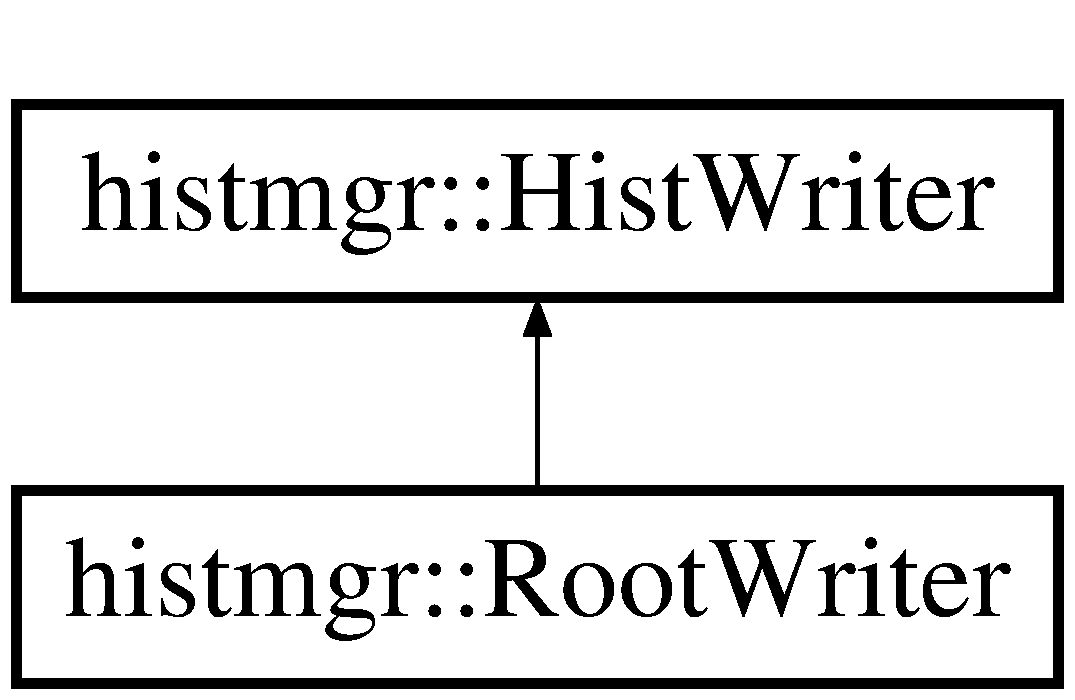
\includegraphics[height=2.000000cm]{classhistmgr_1_1HistWriter}
\end{center}
\end{figure}
\subsection*{Public Member Functions}
\begin{DoxyCompactItemize}
\item 
virtual bool {\bf enter\-Dir} (const std\-::string \&name, Bool\-\_\-t create=false)=0
\begin{DoxyCompactList}\small\item\em Enter a subdirectory in the file. \end{DoxyCompactList}\item 
virtual void {\bf up\-Dir} ()=0\label{classhistmgr_1_1HistWriter_af4a84b802e1617ac850eb828f5d6a644}

\begin{DoxyCompactList}\small\item\em Go up one directory level. \end{DoxyCompactList}\item 
virtual void {\bf write\-To\-Current\-Dir} (const {\bf Float\-Histogram1\-D} \&hist, const std\-::string \&name)=0
\begin{DoxyCompactList}\small\item\em Write the given histogram to a R\-O\-O\-T file. \end{DoxyCompactList}\item 
virtual void {\bf write\-To\-Current\-Dir} (const {\bf Float\-Histogram2\-D} \&hist, const std\-::string \&name)=0
\begin{DoxyCompactList}\small\item\em Write the given histogram to a R\-O\-O\-T file. \end{DoxyCompactList}\item 
virtual void {\bfseries write\-To\-Current\-Dir} (const E\-V\-E\-N\-T\-::\-L\-C\-Generic\-Object $\ast$array\-\_\-x, const E\-V\-E\-N\-T\-::\-L\-C\-Generic\-Object $\ast$array\-\_\-y, const E\-V\-E\-N\-T\-::\-L\-C\-Generic\-Object $\ast$array\-\_\-ey, const std\-::string \&name)=0\label{classhistmgr_1_1HistWriter_a3d8cb01d364fb517626b4b5bb990b9d1}

\end{DoxyCompactItemize}


\subsection{Detailed Description}
Abstract interface of a class to write histograms to disk. 

\begin{DoxySeeAlso}{See Also}
\doxyref{Root\-Writer}{p.}{classhistmgr_1_1RootWriter}. 
\end{DoxySeeAlso}


Definition at line 16 of file Hist\-Writer.\-hh.



\subsection{Member Function Documentation}
\index{histmgr\-::\-Hist\-Writer@{histmgr\-::\-Hist\-Writer}!enter\-Dir@{enter\-Dir}}
\index{enter\-Dir@{enter\-Dir}!histmgr::HistWriter@{histmgr\-::\-Hist\-Writer}}
\subsubsection[{enter\-Dir}]{\setlength{\rightskip}{0pt plus 5cm}virtual bool histmgr\-::\-Hist\-Writer\-::enter\-Dir (
\begin{DoxyParamCaption}
\item[{const std\-::string \&}]{name, }
\item[{Bool\-\_\-t}]{create = {\ttfamily false}}
\end{DoxyParamCaption}
)\hspace{0.3cm}{\ttfamily [pure virtual]}}\label{classhistmgr_1_1HistWriter_adbdbc5948a21d31ee3ab9ff2e3ba1999}


Enter a subdirectory in the file. 


\begin{DoxyParams}{Parameters}
{\em name} & the name of the sub directory \\
\hline
{\em create} & set to true if non existing directories shall be created \\
\hline
\end{DoxyParams}
\begin{DoxyReturn}{Returns}
true incase the directory exists 
\end{DoxyReturn}
\index{histmgr\-::\-Hist\-Writer@{histmgr\-::\-Hist\-Writer}!write\-To\-Current\-Dir@{write\-To\-Current\-Dir}}
\index{write\-To\-Current\-Dir@{write\-To\-Current\-Dir}!histmgr::HistWriter@{histmgr\-::\-Hist\-Writer}}
\subsubsection[{write\-To\-Current\-Dir}]{\setlength{\rightskip}{0pt plus 5cm}virtual void histmgr\-::\-Hist\-Writer\-::write\-To\-Current\-Dir (
\begin{DoxyParamCaption}
\item[{const {\bf Float\-Histogram1\-D} \&}]{hist, }
\item[{const std\-::string \&}]{name}
\end{DoxyParamCaption}
)\hspace{0.3cm}{\ttfamily [pure virtual]}}\label{classhistmgr_1_1HistWriter_ad9bdd8f2a07d67c39bb0e09e79009aa5}


Write the given histogram to a R\-O\-O\-T file. 


\begin{DoxyParams}{Parameters}
{\em hist} & reference to the histogram \\
\hline
{\em name} & the name given to the histogram \\
\hline
\end{DoxyParams}


Implemented in {\bf histmgr\-::\-Root\-Writer} \doxyref{}{p.}{classhistmgr_1_1RootWriter_a14f07347e735118a227788b8a4c5a172}.

\index{histmgr\-::\-Hist\-Writer@{histmgr\-::\-Hist\-Writer}!write\-To\-Current\-Dir@{write\-To\-Current\-Dir}}
\index{write\-To\-Current\-Dir@{write\-To\-Current\-Dir}!histmgr::HistWriter@{histmgr\-::\-Hist\-Writer}}
\subsubsection[{write\-To\-Current\-Dir}]{\setlength{\rightskip}{0pt plus 5cm}virtual void histmgr\-::\-Hist\-Writer\-::write\-To\-Current\-Dir (
\begin{DoxyParamCaption}
\item[{const {\bf Float\-Histogram2\-D} \&}]{hist, }
\item[{const std\-::string \&}]{name}
\end{DoxyParamCaption}
)\hspace{0.3cm}{\ttfamily [pure virtual]}}\label{classhistmgr_1_1HistWriter_a3c4e7228abcd2fe54ec6748aae6407c2}


Write the given histogram to a R\-O\-O\-T file. 


\begin{DoxyParams}{Parameters}
{\em hist} & reference to the histogram \\
\hline
{\em name} & the name given to the histogram \\
\hline
\end{DoxyParams}


Implemented in {\bf histmgr\-::\-Root\-Writer} \doxyref{}{p.}{classhistmgr_1_1RootWriter_a6031ddaa5a402ae73f624fb3ea2e5970}.



The documentation for this class was generated from the following file\-:\begin{DoxyCompactItemize}
\item 
Hist\-Writer.\-hh\end{DoxyCompactItemize}

\section{histmgr\-:\-:Hist\-Writer\-Kit Class Reference}
\label{classhistmgr_1_1HistWriterKit}\index{histmgr\-::\-Hist\-Writer\-Kit@{histmgr\-::\-Hist\-Writer\-Kit}}


Abstract interface of a histogram writer kit.  




{\ttfamily \#include $<$Hist\-Writer\-Kit.\-hh$>$}

Inheritance diagram for histmgr\-:\-:Hist\-Writer\-Kit\-:\begin{figure}[H]
\begin{center}
\leavevmode
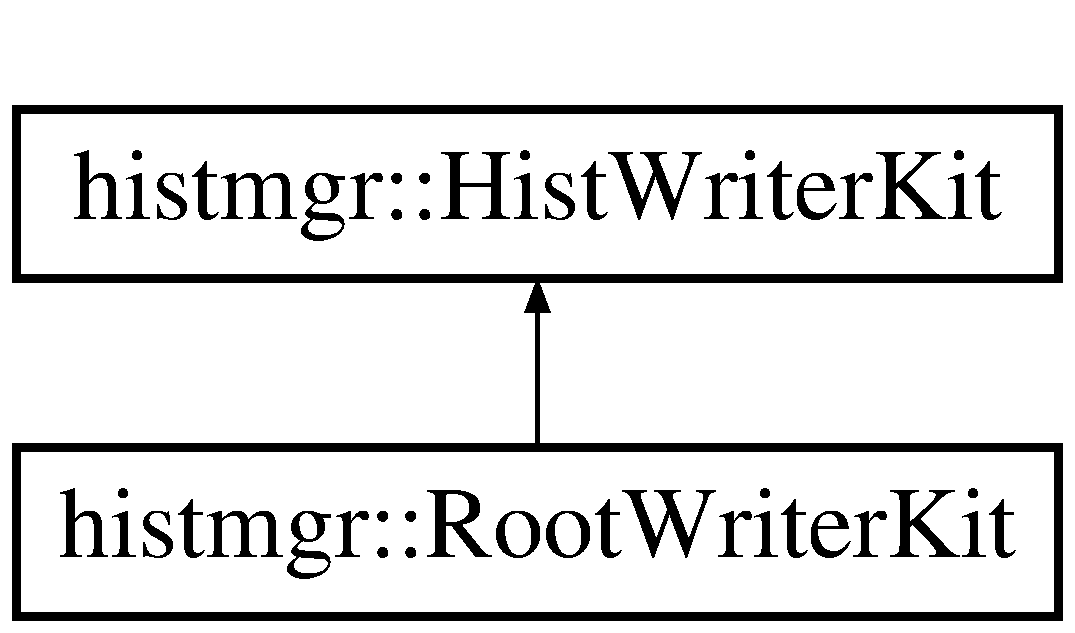
\includegraphics[height=2.000000cm]{classhistmgr_1_1HistWriterKit}
\end{center}
\end{figure}
\subsection*{Public Member Functions}
\begin{DoxyCompactItemize}
\item 
virtual {\bf $\sim$\-Hist\-Writer\-Kit} ()
\begin{DoxyCompactList}\small\item\em Destructor. \end{DoxyCompactList}\item 
virtual {\bf Hist\-Writer} $\ast$ {\bf create\-Writer} (const std\-::string \&name)=0
\begin{DoxyCompactList}\small\item\em create a histogram write. \end{DoxyCompactList}\end{DoxyCompactItemize}


\subsection{Detailed Description}
Abstract interface of a histogram writer kit. 

The writer kit is used to create the actual histogram writer. \begin{DoxySeeAlso}{See Also}
\doxyref{Root\-Writer\-Kit}{p.}{classhistmgr_1_1RootWriterKit} 
\end{DoxySeeAlso}


Definition at line 13 of file Hist\-Writer\-Kit.\-hh.



\subsection{Constructor \& Destructor Documentation}
\index{histmgr\-::\-Hist\-Writer\-Kit@{histmgr\-::\-Hist\-Writer\-Kit}!$\sim$\-Hist\-Writer\-Kit@{$\sim$\-Hist\-Writer\-Kit}}
\index{$\sim$\-Hist\-Writer\-Kit@{$\sim$\-Hist\-Writer\-Kit}!histmgr::HistWriterKit@{histmgr\-::\-Hist\-Writer\-Kit}}
\subsubsection[{$\sim$\-Hist\-Writer\-Kit}]{\setlength{\rightskip}{0pt plus 5cm}virtual histmgr\-::\-Hist\-Writer\-Kit\-::$\sim$\-Hist\-Writer\-Kit (
\begin{DoxyParamCaption}
{}
\end{DoxyParamCaption}
)\hspace{0.3cm}{\ttfamily [inline]}, {\ttfamily [virtual]}}\label{classhistmgr_1_1HistWriterKit_aa3c62231adb0f1f95295d27e559009a3}


Destructor. 

Abstract classes need a virtual destructor. 

Definition at line 19 of file Hist\-Writer\-Kit.\-hh.



\subsection{Member Function Documentation}
\index{histmgr\-::\-Hist\-Writer\-Kit@{histmgr\-::\-Hist\-Writer\-Kit}!create\-Writer@{create\-Writer}}
\index{create\-Writer@{create\-Writer}!histmgr::HistWriterKit@{histmgr\-::\-Hist\-Writer\-Kit}}
\subsubsection[{create\-Writer}]{\setlength{\rightskip}{0pt plus 5cm}virtual {\bf Hist\-Writer}$\ast$ histmgr\-::\-Hist\-Writer\-Kit\-::create\-Writer (
\begin{DoxyParamCaption}
\item[{const std\-::string \&}]{name}
\end{DoxyParamCaption}
)\hspace{0.3cm}{\ttfamily [pure virtual]}}\label{classhistmgr_1_1HistWriterKit_a4e07d5baf676d4af138d09f2e92b4001}


create a histogram write. 


\begin{DoxyParams}{Parameters}
{\em name} & the name of the file to which the histograms should be written \\
\hline
\end{DoxyParams}
\begin{DoxyReturn}{Returns}
a pointer a histogram writer which should be ready to write histograms. 
\end{DoxyReturn}


Implemented in {\bf histmgr\-::\-Root\-Writer\-Kit} \doxyref{}{p.}{classhistmgr_1_1RootWriterKit_a480fb8728c4592098a59344922a58c71}.



The documentation for this class was generated from the following file\-:\begin{DoxyCompactItemize}
\item 
Hist\-Writer\-Kit.\-hh\end{DoxyCompactItemize}

\section{C\-A\-L\-I\-C\-E\-:\-:Hold\-Scan\-Analysis Class Reference}
\label{classCALICE_1_1HoldScanAnalysis}\index{C\-A\-L\-I\-C\-E\-::\-Hold\-Scan\-Analysis@{C\-A\-L\-I\-C\-E\-::\-Hold\-Scan\-Analysis}}


Create Signal histograms per pad of all hits of all reconstructed clusters.  




{\ttfamily \#include $<$Hold\-Scan\-Analysis.\-hh$>$}

Inheritance diagram for C\-A\-L\-I\-C\-E\-:\-:Hold\-Scan\-Analysis\-:\begin{figure}[H]
\begin{center}
\leavevmode
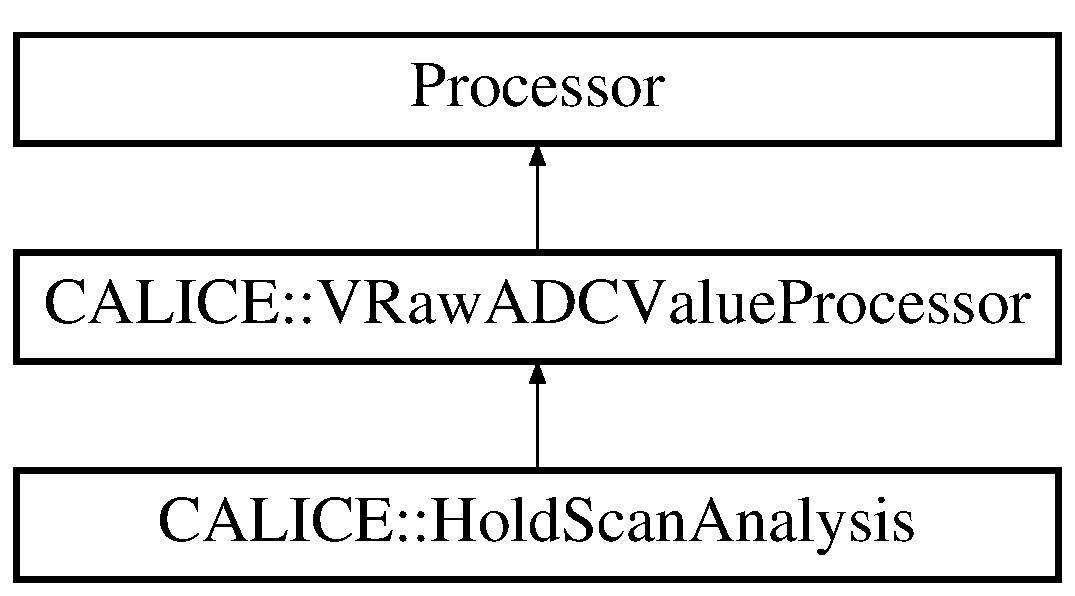
\includegraphics[height=3.000000cm]{classCALICE_1_1HoldScanAnalysis}
\end{center}
\end{figure}
\subsection*{Public Member Functions}
\begin{DoxyCompactItemize}
\item 
Processor $\ast$ {\bfseries new\-Processor} ()\label{classCALICE_1_1HoldScanAnalysis_ad5990596dee1b8767277be9526521161}

\item 
void {\bf init} ()
\begin{DoxyCompactList}\small\item\em Called at the begin of the job before anything is read. \end{DoxyCompactList}\item 
void {\bf process\-Run\-Header} (L\-C\-Run\-Header $\ast$run)
\begin{DoxyCompactList}\small\item\em Called for every run, e.\-g. \end{DoxyCompactList}\item 
void {\bf process\-Event} (L\-C\-Event $\ast$evt\-P)
\begin{DoxyCompactList}\small\item\em Called for every event -\/ the working horse. \end{DoxyCompactList}\item 
void {\bfseries end} ()\label{classCALICE_1_1HoldScanAnalysis_a13ed162b61891ce64fb6cfff41719b18}

\end{DoxyCompactItemize}
\subsection*{Protected Types}
\begin{DoxyCompactItemize}
\item 
enum {\bfseries E\-Hist\-Type} \{ {\bfseries k\-Hist\-Signal\-Per\-Hold\-Value}, 
{\bfseries k\-Hist\-Total\-Signal\-Per\-Hold\-Value}, 
{\bfseries k\-N\-Hist}
 \}
\end{DoxyCompactItemize}
\subsection*{Protected Member Functions}
\begin{DoxyCompactItemize}
\item 
void {\bf create\-Histograms} ()
\begin{DoxyCompactList}\small\item\em create and register histogram collections. \end{DoxyCompactList}\item 
void {\bf fe\-Conf\-Changed} (E\-V\-E\-N\-T\-::\-L\-C\-Collection $\ast$col)\label{classCALICE_1_1HoldScanAnalysis_a59d01b5f9111a355a98087f22edda54c}

\begin{DoxyCompactList}\small\item\em Handle changes of Fe configuration data. \end{DoxyCompactList}\item 
void {\bfseries module\-Type\-Changed} (lcio\-::\-L\-C\-Collection $\ast$col)\label{classCALICE_1_1HoldScanAnalysis_a13f67124dfbac5a43384720d728cd79d}

\item 
void {\bfseries module\-Location\-Changed} (lcio\-::\-L\-C\-Collection $\ast$col)\label{classCALICE_1_1HoldScanAnalysis_ac7853b9f5030f2cffff1763c803c6ed4}

\item 
void {\bfseries module\-Connection\-Changed} (lcio\-::\-L\-C\-Collection $\ast$col)\label{classCALICE_1_1HoldScanAnalysis_a8b1ef0f8b1806f814f738179a0c94773}

\end{DoxyCompactItemize}
\subsection*{Protected Attributes}
\begin{DoxyCompactItemize}
\item 
Float\-Vec {\bf \-\_\-signal\-Hist\-Par}
\begin{DoxyCompactList}\small\item\em binning of the per hold value histograms. \end{DoxyCompactList}\item 
std\-::string {\bfseries \-\_\-cluster\-Col\-Name}\label{classCALICE_1_1HoldScanAnalysis_a821525b65e2b0658befe4572ff2b5a5b}

\item 
std\-::string {\bfseries \-\_\-fe\-Conf\-Col\-Name}\label{classCALICE_1_1HoldScanAnalysis_a05396b051321b994175ab5c26bc36ccd}

\item 
{\bf histmgr\-::\-Key\-\_\-t} {\bf \-\_\-hist\-Group\-Key}
\begin{DoxyCompactList}\small\item\em Key for the histogram group. \end{DoxyCompactList}\item 
int {\bf \-\_\-n\-Hist\-Max}\label{classCALICE_1_1HoldScanAnalysis_a9d4b44b172ef158fc0cc865ff00c8200}

\begin{DoxyCompactList}\small\item\em Maximum number of hold values for which signal histograms can be created (parameter) \end{DoxyCompactList}\item 
int {\bf \-\_\-min\-Number\-Of\-Hits}
\begin{DoxyCompactList}\small\item\em Minimum number of hits of accepted clusters (parameter). \end{DoxyCompactList}\item 
Float\-\_\-t {\bf \-\_\-min\-Cluster\-Signal}
\begin{DoxyCompactList}\small\item\em Minimum signal of accepted clusters (parameter). \end{DoxyCompactList}\item 
Conditions\-Change\-Delegator\\*
$<$ {\bf Hold\-Scan\-Analysis} $>$ {\bfseries \-\_\-fe\-Conf\-Change}\label{classCALICE_1_1HoldScanAnalysis_abc178bb058507f39db6a6b9434153141}

\item 
{\bf Module\-Index\-Reverse\-Lookup} {\bfseries \-\_\-index\-Lookup}\label{classCALICE_1_1HoldScanAnalysis_a19e9e6c81508e9e2a993f980448b0255}

\item 
L\-C\-Collection $\ast$ {\bfseries \-\_\-n\-Hits\-Histogram}\label{classCALICE_1_1HoldScanAnalysis_a62943d737949a663b3ea9583adeb56d8}

\item 
L\-C\-Collection $\ast$ {\bfseries \-\_\-cluster\-Signal\-Histogram}\label{classCALICE_1_1HoldScanAnalysis_accdd2109f252c0a48d601dd3f675cbf1}

\item 
L\-C\-Collection $\ast$ {\bfseries \-\_\-hold\-Value\-Container}\label{classCALICE_1_1HoldScanAnalysis_aee61abfbb2658d6b4e184604e58b6dcb}

\item 
{\bf histmgr\-::\-Key\-\_\-t} {\bfseries \-\_\-hist\-Key} [k\-N\-Hist]\label{classCALICE_1_1HoldScanAnalysis_a2d3c6efe1f8a31b54998e8fc548db0e4}

\item 
U\-Int\-\_\-t {\bfseries \-\_\-n\-Hist}\label{classCALICE_1_1HoldScanAnalysis_ac9cacb21c7c4e771c1f288bb68e390d2}

\item 
std\-::map$<$ int, U\-Int\-\_\-t $>$ {\bfseries \-\_\-hold\-Start\-Map}\label{classCALICE_1_1HoldScanAnalysis_a9f62a744912af880d609661590b59cb0}

\item 
std\-::vector$<$ U\-Int\-\_\-t $>$ {\bfseries \-\_\-histogram\-Index}\label{classCALICE_1_1HoldScanAnalysis_a4d69205cdc09cb052ac036b530c7ae41}

\item 
U\-Int\-\_\-t {\bfseries \-\_\-n\-Clusters}\label{classCALICE_1_1HoldScanAnalysis_a1a8fa6dbaaabcf4e2059a828bd6c05e1}

\item 
U\-Int\-\_\-t {\bfseries \-\_\-n\-Missing\-Hold\-Changes}\label{classCALICE_1_1HoldScanAnalysis_afea5db3b613767acb605be6f4f6a20ca}

\item 
U\-Int\-\_\-t {\bfseries \-\_\-module\-Index\-Out\-Of\-Range}\label{classCALICE_1_1HoldScanAnalysis_ae9a8dcd16dde44f63bc083ceabd98616}

\item 
U\-Int\-\_\-t {\bfseries \-\_\-n\-Beam\-Or\-Cosmics\-Events}\label{classCALICE_1_1HoldScanAnalysis_aae4c0032da689c8bd59a62dc1a9fb23e}

\item 
U\-Int\-\_\-t {\bfseries \-\_\-current\-Common\-Hold\-Start}\label{classCALICE_1_1HoldScanAnalysis_a9bc44aaf4bbc5147174b8e3d813df954}

\end{DoxyCompactItemize}


\subsection{Detailed Description}
Create Signal histograms per pad of all hits of all reconstructed clusters. 

This class derives from \doxyref{V\-Raw\-A\-D\-C\-Value\-Processor}{p.}{classCALICE_1_1VRawADCValueProcessor}, since the information about the detector is needed to setup the signal histograms. 

Definition at line 25 of file Hold\-Scan\-Analysis.\-hh.



\subsection{Member Function Documentation}
\index{C\-A\-L\-I\-C\-E\-::\-Hold\-Scan\-Analysis@{C\-A\-L\-I\-C\-E\-::\-Hold\-Scan\-Analysis}!create\-Histograms@{create\-Histograms}}
\index{create\-Histograms@{create\-Histograms}!CALICE::HoldScanAnalysis@{C\-A\-L\-I\-C\-E\-::\-Hold\-Scan\-Analysis}}
\subsubsection[{create\-Histograms}]{\setlength{\rightskip}{0pt plus 5cm}void C\-A\-L\-I\-C\-E\-::\-Hold\-Scan\-Analysis\-::create\-Histograms (
\begin{DoxyParamCaption}
{}
\end{DoxyParamCaption}
)\hspace{0.3cm}{\ttfamily [protected]}}\label{classCALICE_1_1HoldScanAnalysis_af9b442f35ad6b560ecf6736fdaa39314}


create and register histogram collections. 



Definition at line 105 of file Hold\-Scan\-Analysis.\-cc.



References histmgr\-::\-Hist\-Mgr\-::create\-Histogram\-Group(), and histmgr\-::\-Hist\-Mgr\-::create\-Histograms().

\index{C\-A\-L\-I\-C\-E\-::\-Hold\-Scan\-Analysis@{C\-A\-L\-I\-C\-E\-::\-Hold\-Scan\-Analysis}!init@{init}}
\index{init@{init}!CALICE::HoldScanAnalysis@{C\-A\-L\-I\-C\-E\-::\-Hold\-Scan\-Analysis}}
\subsubsection[{init}]{\setlength{\rightskip}{0pt plus 5cm}void C\-A\-L\-I\-C\-E\-::\-Hold\-Scan\-Analysis\-::init (
\begin{DoxyParamCaption}
{}
\end{DoxyParamCaption}
)}\label{classCALICE_1_1HoldScanAnalysis_aa879bdea19cfbf5e5533174dc7a24c0f}


Called at the begin of the job before anything is read. 

Use to initialize the processor, e.\-g. book histograms. 

Definition at line 128 of file Hold\-Scan\-Analysis.\-cc.



References histmgr\-::\-Hist\-Mgr\-::create\-Histograms().

\index{C\-A\-L\-I\-C\-E\-::\-Hold\-Scan\-Analysis@{C\-A\-L\-I\-C\-E\-::\-Hold\-Scan\-Analysis}!process\-Event@{process\-Event}}
\index{process\-Event@{process\-Event}!CALICE::HoldScanAnalysis@{C\-A\-L\-I\-C\-E\-::\-Hold\-Scan\-Analysis}}
\subsubsection[{process\-Event}]{\setlength{\rightskip}{0pt plus 5cm}void C\-A\-L\-I\-C\-E\-::\-Hold\-Scan\-Analysis\-::process\-Event (
\begin{DoxyParamCaption}
\item[{L\-C\-Event $\ast$}]{evt\-P}
\end{DoxyParamCaption}
)}\label{classCALICE_1_1HoldScanAnalysis_ae6c771d770ca5b456f82efe1e8c19d13}


Called for every event -\/ the working horse. 



Definition at line 161 of file Hold\-Scan\-Analysis.\-cc.



References histmgr\-::\-Float\-Histogram1\-D\-::fill(), histmgr\-::\-Hist\-Mgr\-::get\-Histogram\-Collection(), and histmgr\-::\-Histogram\-Collection\-\_\-t\-::histogram().

\index{C\-A\-L\-I\-C\-E\-::\-Hold\-Scan\-Analysis@{C\-A\-L\-I\-C\-E\-::\-Hold\-Scan\-Analysis}!process\-Run\-Header@{process\-Run\-Header}}
\index{process\-Run\-Header@{process\-Run\-Header}!CALICE::HoldScanAnalysis@{C\-A\-L\-I\-C\-E\-::\-Hold\-Scan\-Analysis}}
\subsubsection[{process\-Run\-Header}]{\setlength{\rightskip}{0pt plus 5cm}void C\-A\-L\-I\-C\-E\-::\-Hold\-Scan\-Analysis\-::process\-Run\-Header (
\begin{DoxyParamCaption}
\item[{L\-C\-Run\-Header $\ast$}]{run}
\end{DoxyParamCaption}
)\hspace{0.3cm}{\ttfamily [inline]}}\label{classCALICE_1_1HoldScanAnalysis_ae23825d881a551a473319f0dc518bd20}


Called for every run, e.\-g. 

overwrite to initialize run dependent histograms. 

Definition at line 43 of file Hold\-Scan\-Analysis.\-hh.



\subsection{Field Documentation}
\index{C\-A\-L\-I\-C\-E\-::\-Hold\-Scan\-Analysis@{C\-A\-L\-I\-C\-E\-::\-Hold\-Scan\-Analysis}!\-\_\-hist\-Group\-Key@{\-\_\-hist\-Group\-Key}}
\index{\-\_\-hist\-Group\-Key@{\-\_\-hist\-Group\-Key}!CALICE::HoldScanAnalysis@{C\-A\-L\-I\-C\-E\-::\-Hold\-Scan\-Analysis}}
\subsubsection[{\-\_\-hist\-Group\-Key}]{\setlength{\rightskip}{0pt plus 5cm}{\bf histmgr\-::\-Key\-\_\-t} C\-A\-L\-I\-C\-E\-::\-Hold\-Scan\-Analysis\-::\-\_\-hist\-Group\-Key\hspace{0.3cm}{\ttfamily [protected]}}\label{classCALICE_1_1HoldScanAnalysis_a85e98fffce43215e0edabf5afc2b346b}


Key for the histogram group. 



Definition at line 63 of file Hold\-Scan\-Analysis.\-hh.

\index{C\-A\-L\-I\-C\-E\-::\-Hold\-Scan\-Analysis@{C\-A\-L\-I\-C\-E\-::\-Hold\-Scan\-Analysis}!\-\_\-min\-Cluster\-Signal@{\-\_\-min\-Cluster\-Signal}}
\index{\-\_\-min\-Cluster\-Signal@{\-\_\-min\-Cluster\-Signal}!CALICE::HoldScanAnalysis@{C\-A\-L\-I\-C\-E\-::\-Hold\-Scan\-Analysis}}
\subsubsection[{\-\_\-min\-Cluster\-Signal}]{\setlength{\rightskip}{0pt plus 5cm}Float\-\_\-t C\-A\-L\-I\-C\-E\-::\-Hold\-Scan\-Analysis\-::\-\_\-min\-Cluster\-Signal\hspace{0.3cm}{\ttfamily [protected]}}\label{classCALICE_1_1HoldScanAnalysis_aaa4aecb1608fddf7a791e6a00e8d9aac}


Minimum signal of accepted clusters (parameter). 



Definition at line 68 of file Hold\-Scan\-Analysis.\-hh.

\index{C\-A\-L\-I\-C\-E\-::\-Hold\-Scan\-Analysis@{C\-A\-L\-I\-C\-E\-::\-Hold\-Scan\-Analysis}!\-\_\-min\-Number\-Of\-Hits@{\-\_\-min\-Number\-Of\-Hits}}
\index{\-\_\-min\-Number\-Of\-Hits@{\-\_\-min\-Number\-Of\-Hits}!CALICE::HoldScanAnalysis@{C\-A\-L\-I\-C\-E\-::\-Hold\-Scan\-Analysis}}
\subsubsection[{\-\_\-min\-Number\-Of\-Hits}]{\setlength{\rightskip}{0pt plus 5cm}int C\-A\-L\-I\-C\-E\-::\-Hold\-Scan\-Analysis\-::\-\_\-min\-Number\-Of\-Hits\hspace{0.3cm}{\ttfamily [protected]}}\label{classCALICE_1_1HoldScanAnalysis_aa13f8c6d7a4c85a4a7eb70c1ec9a02a0}


Minimum number of hits of accepted clusters (parameter). 



Definition at line 67 of file Hold\-Scan\-Analysis.\-hh.

\index{C\-A\-L\-I\-C\-E\-::\-Hold\-Scan\-Analysis@{C\-A\-L\-I\-C\-E\-::\-Hold\-Scan\-Analysis}!\-\_\-signal\-Hist\-Par@{\-\_\-signal\-Hist\-Par}}
\index{\-\_\-signal\-Hist\-Par@{\-\_\-signal\-Hist\-Par}!CALICE::HoldScanAnalysis@{C\-A\-L\-I\-C\-E\-::\-Hold\-Scan\-Analysis}}
\subsubsection[{\-\_\-signal\-Hist\-Par}]{\setlength{\rightskip}{0pt plus 5cm}Float\-Vec C\-A\-L\-I\-C\-E\-::\-Hold\-Scan\-Analysis\-::\-\_\-signal\-Hist\-Par\hspace{0.3cm}{\ttfamily [protected]}}\label{classCALICE_1_1HoldScanAnalysis_af5d6fa8f5fce15286a9fbb3390f35391}


binning of the per hold value histograms. 



Definition at line 56 of file Hold\-Scan\-Analysis.\-hh.



The documentation for this class was generated from the following files\-:\begin{DoxyCompactItemize}
\item 
Hold\-Scan\-Analysis.\-hh\item 
Hold\-Scan\-Analysis.\-cc\end{DoxyCompactItemize}

\section{C\-A\-L\-I\-C\-E\-:\-:Integrated\-Hcal\-Calibration\-Processor Class Reference}
\label{classCALICE_1_1IntegratedHcalCalibrationProcessor}\index{C\-A\-L\-I\-C\-E\-::\-Integrated\-Hcal\-Calibration\-Processor@{C\-A\-L\-I\-C\-E\-::\-Integrated\-Hcal\-Calibration\-Processor}}


The Ahcal calibration processor.  




{\ttfamily \#include $<$Integrated\-Hcal\-Calibration\-Processor.\-hh$>$}

Inheritance diagram for C\-A\-L\-I\-C\-E\-:\-:Integrated\-Hcal\-Calibration\-Processor\-:\begin{figure}[H]
\begin{center}
\leavevmode
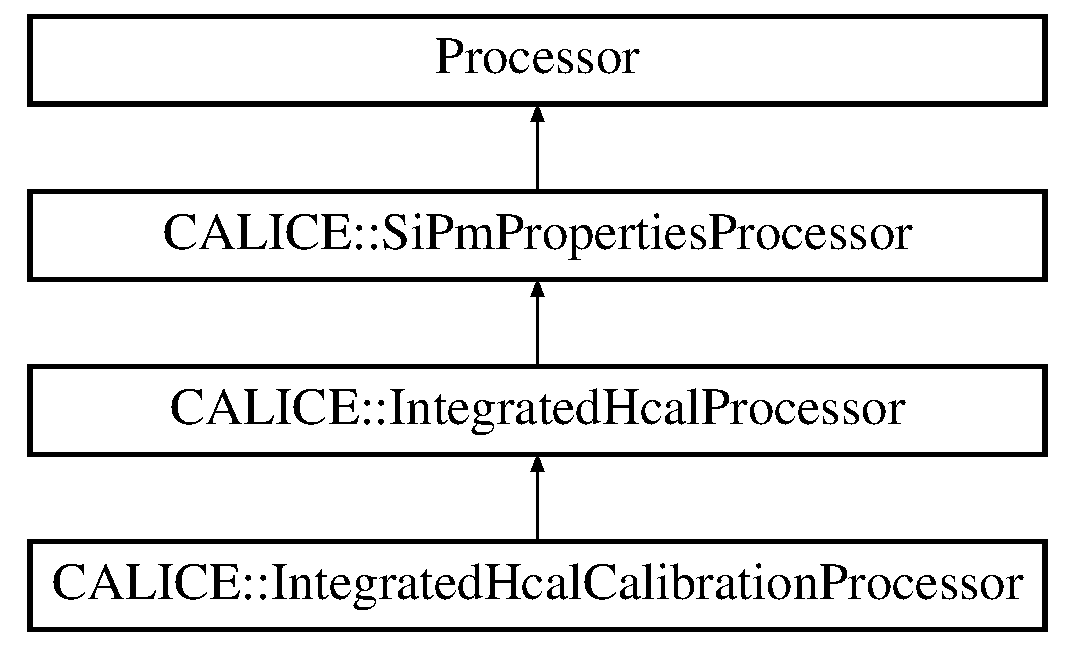
\includegraphics[height=4.000000cm]{classCALICE_1_1IntegratedHcalCalibrationProcessor}
\end{center}
\end{figure}
\subsection*{Public Member Functions}
\begin{DoxyCompactItemize}
\item 
{\bf Integrated\-Hcal\-Calibration\-Processor} $\ast$ {\bfseries new\-Processor} ()\label{classCALICE_1_1IntegratedHcalCalibrationProcessor_a598bbbd1a328ce27442d3a9d026b9867}

\item 
virtual void {\bfseries init} ()\label{classCALICE_1_1IntegratedHcalCalibrationProcessor_afcb4ac8fef8a5bcc1fd5ae4b8620af85}

\item 
virtual void {\bfseries process\-Event} (lcio\-::\-L\-C\-Event $\ast$evt)\label{classCALICE_1_1IntegratedHcalCalibrationProcessor_acf33ed983e6e78fc7c70c5a0082d9cf0}

\item 
virtual void {\bfseries end} ()\label{classCALICE_1_1IntegratedHcalCalibrationProcessor_a8f73d365b94979a80808dc903cfc9c00}

\end{DoxyCompactItemize}
\subsection*{Protected Attributes}
\begin{DoxyCompactItemize}
\item 
std\-::string {\bfseries \-\_\-input\-Col\-Name}\label{classCALICE_1_1IntegratedHcalCalibrationProcessor_ad9b166089f6501b37a89d13c0a25bb2e}

\item 
std\-::string {\bfseries \-\_\-output\-Col\-Name}\label{classCALICE_1_1IntegratedHcalCalibrationProcessor_a7b272632e6fd4e847dbb9dee88b7ceb8}

\item 
int {\bfseries \-\_\-zero\-Suppression}\label{classCALICE_1_1IntegratedHcalCalibrationProcessor_a50776188b69d33bec8a734fcc082b22b}

\item 
float {\bfseries \-\_\-significance\-Cut}\label{classCALICE_1_1IntegratedHcalCalibrationProcessor_a0f9dbdb9a4ebc2b7955679cc64e19636}

\item 
int {\bfseries \-\_\-skip\-Pedestals}\label{classCALICE_1_1IntegratedHcalCalibrationProcessor_a55d12f2aaaab3f29212109bfde96b759}

\item 
int {\bfseries \-\_\-min\-Ped\-Number}\label{classCALICE_1_1IntegratedHcalCalibrationProcessor_a2d709e61047bcb4cfbad62fde9d140df}

\item 
int {\bfseries \-\_\-ped\-Counter}\label{classCALICE_1_1IntegratedHcalCalibrationProcessor_ae916fee0673eb80e5acc3fdb73adc24a}

\item 
int {\bfseries \-\_\-pedestal\-Subtraction}\label{classCALICE_1_1IntegratedHcalCalibrationProcessor_a1c0d957bc70006c6f071d53799da2c5f}

\item 
float {\bfseries \-\_\-mip\-Cut}\label{classCALICE_1_1IntegratedHcalCalibrationProcessor_a5670d938f278f3d4d66fbf481f0ec4c4}

\item 
bool {\bfseries \-\_\-do\-Saturation\-Correction}\label{classCALICE_1_1IntegratedHcalCalibrationProcessor_aa022999f9178f6b1a8ea7575362fe8d1}

\item 
unsigned long {\bfseries \-\_\-hit\-Counter}\label{classCALICE_1_1IntegratedHcalCalibrationProcessor_a68d73faf87415a4af9a6e3a0f35476e8}

\item 
unsigned long {\bfseries \-\_\-invalid\-M\-I\-P\-Counter}\label{classCALICE_1_1IntegratedHcalCalibrationProcessor_a8abdbee26c81f4aa9336ff5b07ef9cde}

\item 
unsigned long {\bfseries \-\_\-invalid\-Saturation\-Correction\-Counter}\label{classCALICE_1_1IntegratedHcalCalibrationProcessor_a34510ab0a63023762ef2eb82b3e57587}

\item 
unsigned long {\bfseries \-\_\-saturation\-Counter}\label{classCALICE_1_1IntegratedHcalCalibrationProcessor_aaf95bbbe9b7d96f34c900eaedc800a15}

\item 
unsigned long {\bfseries \-\_\-event\-Counter}\label{classCALICE_1_1IntegratedHcalCalibrationProcessor_a244b0feb4e3c0dbc80cdb881d33531a0}

\item 
std\-::map$<$ unsigned, unsigned $>$ {\bfseries \-\_\-invalid\-M\-I\-P\-Calibrations}\label{classCALICE_1_1IntegratedHcalCalibrationProcessor_a865d6e28f28638bf3af375cb31555db4}

\item 
std\-::map$<$ unsigned, unsigned $>$ {\bfseries \-\_\-invalid\-Saturation\-Corrections}\label{classCALICE_1_1IntegratedHcalCalibrationProcessor_a1a8724c11472e790d565b76438f3d6cc}

\item 
std\-::map$<$ unsigned, unsigned $>$ {\bfseries \-\_\-saturations}\label{classCALICE_1_1IntegratedHcalCalibrationProcessor_aec10a6498f7f035f9909bfc1d87aeeb7}

\item 
double {\bfseries \-\_\-ped\-Sum} [H\-C\-A\-L\-\_\-\-N\-\_\-\-M\-O\-D+1][H\-C\-A\-L\-\_\-\-N\-\_\-\-C\-E\-L\-L]\label{classCALICE_1_1IntegratedHcalCalibrationProcessor_a62f50a5f4d2f7b8f1a346c01f6b0d8df}

\item 
double {\bfseries \-\_\-ped\-Sum\-Square} [H\-C\-A\-L\-\_\-\-N\-\_\-\-M\-O\-D+1][H\-C\-A\-L\-\_\-\-N\-\_\-\-C\-E\-L\-L]\label{classCALICE_1_1IntegratedHcalCalibrationProcessor_a452abcc49cbfe1c24f9671d1864c39a8}

\item 
unsigned {\bfseries \-\_\-ped\-Num} [H\-C\-A\-L\-\_\-\-N\-\_\-\-M\-O\-D+1][H\-C\-A\-L\-\_\-\-N\-\_\-\-C\-E\-L\-L]\label{classCALICE_1_1IntegratedHcalCalibrationProcessor_aadb43e8133ddf7a6fc74f6812fa65d53}

\item 
float {\bfseries \-\_\-ped} [H\-C\-A\-L\-\_\-\-N\-\_\-\-M\-O\-D+1][H\-C\-A\-L\-\_\-\-N\-\_\-\-C\-E\-L\-L]\label{classCALICE_1_1IntegratedHcalCalibrationProcessor_a15da76dd2514ace90b34ec890ee49f3a}

\item 
float {\bfseries \-\_\-ped\-Width} [H\-C\-A\-L\-\_\-\-N\-\_\-\-M\-O\-D+1][H\-C\-A\-L\-\_\-\-N\-\_\-\-C\-E\-L\-L]\label{classCALICE_1_1IntegratedHcalCalibrationProcessor_aaf5121c45f2bd9af321b74d6247186fa}

\item 
float {\bfseries \-\_\-ped\-Error} [H\-C\-A\-L\-\_\-\-N\-\_\-\-M\-O\-D+1][H\-C\-A\-L\-\_\-\-N\-\_\-\-C\-E\-L\-L]\label{classCALICE_1_1IntegratedHcalCalibrationProcessor_aa0fd128f60f5a4b034660f0ed4c5428c}

\end{DoxyCompactItemize}
\subsection*{Additional Inherited Members}


\subsection{Detailed Description}
The Ahcal calibration processor. 

\begin{DoxyAuthor}{Author}
Sebastian Schmidt 
\end{DoxyAuthor}


Definition at line 42 of file Integrated\-Hcal\-Calibration\-Processor.\-hh.



The documentation for this class was generated from the following files\-:\begin{DoxyCompactItemize}
\item 
Integrated\-Hcal\-Calibration\-Processor.\-hh\item 
Integrated\-Hcal\-Calibration\-Processor.\-cc\end{DoxyCompactItemize}

\section{C\-A\-L\-I\-C\-E\-:\-:Integrated\-Hcal\-Processor Class Reference}
\label{classCALICE_1_1IntegratedHcalProcessor}\index{C\-A\-L\-I\-C\-E\-::\-Integrated\-Hcal\-Processor@{C\-A\-L\-I\-C\-E\-::\-Integrated\-Hcal\-Processor}}


Base class for all processors which need a lot of A\-Hcal specific data, like the \doxyref{C\-A\-L\-I\-C\-E\-::\-Integrated\-Hcal\-Calibration\-Processor}{p.}{classCALICE_1_1IntegratedHcalCalibrationProcessor} and the C\-A\-L\-I\-C\-E\-::\-Integrated\-Hcal\-Digitization\-Processor.  




{\ttfamily \#include $<$Integrated\-Hcal\-Processor.\-hh$>$}

Inheritance diagram for C\-A\-L\-I\-C\-E\-:\-:Integrated\-Hcal\-Processor\-:\begin{figure}[H]
\begin{center}
\leavevmode
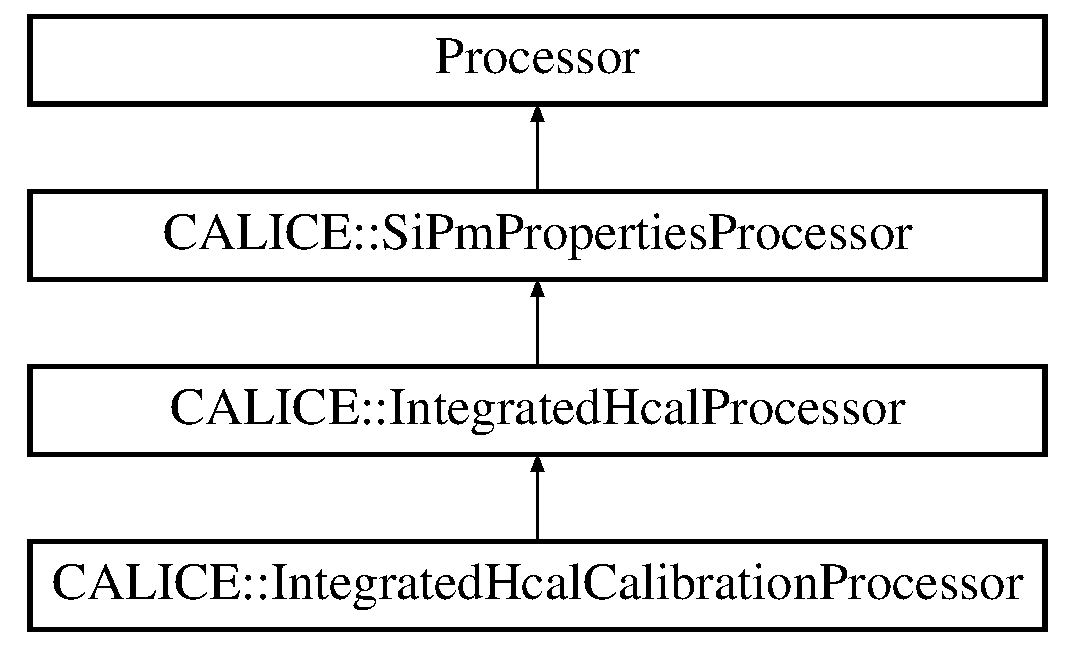
\includegraphics[height=4.000000cm]{classCALICE_1_1IntegratedHcalProcessor}
\end{center}
\end{figure}
\subsection*{Data Structures}
\begin{DoxyCompactItemize}
\item 
struct {\bf Neighbour\-Item}
\begin{DoxyCompactList}\small\item\em int \-\_\-fudge\-Non\-Existing\-Saturation\-Corrections; \end{DoxyCompactList}\end{DoxyCompactItemize}
\subsection*{Public Member Functions}
\begin{DoxyCompactItemize}
\item 
{\bf Integrated\-Hcal\-Processor} (const std\-::string processor\-Name=\char`\"{}Integrated\-Hcal\-Processor\char`\"{})
\begin{DoxyCompactList}\small\item\em \-\_\-gain\-Fit\-Results\-Map(\&\-C\-A\-L\-I\-C\-E\-::\-Linear\-Fit\-Result\-::get\-I\-D), \-\_\-\-Mip\-Fit\-Results\-Map(\&\-C\-A\-L\-I\-C\-E\-::\-Linear\-Fit\-Result\-::get\-I\-D), \end{DoxyCompactList}\item 
virtual {\bf $\sim$\-Integrated\-Hcal\-Processor} ()
\item 
{\bf Integrated\-Hcal\-Processor} $\ast$ {\bfseries new\-Processor} ()\label{classCALICE_1_1IntegratedHcalProcessor_a1756ad865a23dee3410dcca7e3ea6594}

\item 
virtual void {\bf init} ()
\end{DoxyCompactItemize}
\subsection*{Protected Types}
\begin{DoxyCompactItemize}
\item 
typedef std\-::map$<$ unsigned, \\*
std\-::vector$<$ {\bf Neighbour\-Item} $>$ $\ast$ $>$ {\bfseries Neighbour\-Map}\label{classCALICE_1_1IntegratedHcalProcessor_a0bfd2769021f0a1a69ab275249d8bb81}

\end{DoxyCompactItemize}
\subsection*{Protected Member Functions}
\begin{DoxyCompactItemize}
\item 
void {\bf fill\-Temp\-Count\-Maps} (int cell\-I\-D)\label{classCALICE_1_1IntegratedHcalProcessor_af53541acd9828c24c24a915b92eb073e}

\begin{DoxyCompactList}\small\item\em Is used to fill temperature correction statistic maps. \end{DoxyCompactList}\item 
void {\bfseries fill\-Temp\-Count\-Maps} (unsigned module, unsigned chip, unsigned channel)\label{classCALICE_1_1IntegratedHcalProcessor_a1f7f99d2acf5eb86bb88a66f014caf42}

\item 
void {\bf print\-Temp\-Count\-Maps} (std\-::ostream \&out)\label{classCALICE_1_1IntegratedHcalProcessor_aeb33252fcb974978f913ed4e14e65d24}

\begin{DoxyCompactList}\small\item\em Is used to print temperature correction statistic maps. \end{DoxyCompactList}\item 
virtual void {\bf ahc\-Sro\-Mod\-Data\-Col\-Changed} (lcio\-::\-L\-C\-Collection $\ast$col)
\begin{DoxyCompactList}\small\item\em void Integrated\-Hcal\-Processor\-::gain\-Calibration\-Changed(lcio\-::\-L\-C\-Collection$\ast$ col) \{ ifdef H\-C\-A\-L\-R\-E\-C\-O\-\_\-\-D\-E\-B\-U\-G \end{DoxyCompactList}\item 
virtual void {\bfseries temperature\-Sensor\-Calibration\-Changed} (lcio\-::\-L\-C\-Collection $\ast$col)\label{classCALICE_1_1IntegratedHcalProcessor_a789b552c5a5d2b9f98d23d0c0cfb78be}

\item 
virtual void {\bfseries Sipm\-Info\-Changed} (lcio\-::\-L\-C\-Collection $\ast$col)\label{classCALICE_1_1IntegratedHcalProcessor_a7f9eff7025074d0a5a573f62ecdaa198}

\item 
virtual void {\bfseries Sipm\-Saturation\-Changed} (lcio\-::\-L\-C\-Collection $\ast$col)\label{classCALICE_1_1IntegratedHcalProcessor_ab191e86a502f637fc0956f5281a6fae6}

\item 
virtual void {\bfseries Module\-Production\-Changed} (lcio\-::\-L\-C\-Collection $\ast$col)\label{classCALICE_1_1IntegratedHcalProcessor_a762308d52579972a065c7af24afafdb4}

\item 
virtual void {\bfseries module\-Type\-Changed} (lcio\-::\-L\-C\-Collection $\ast$col)\label{classCALICE_1_1IntegratedHcalProcessor_ad82209008f52da453135a2df963e6f98}

\item 
virtual void {\bfseries module\-Location\-Changed} (lcio\-::\-L\-C\-Collection $\ast$col)\label{classCALICE_1_1IntegratedHcalProcessor_ac66500e314f73a864dbddbb78a332ef0}

\item 
virtual void {\bfseries module\-Connection\-Changed} (lcio\-::\-L\-C\-Collection $\ast$col)\label{classCALICE_1_1IntegratedHcalProcessor_a0062408fe85891e299dc2dfd6702c5c5}

\item 
float {\bf get\-Mip} (int Cell\-I\-D)
\begin{DoxyCompactList}\small\item\em Use this function to get the Mip constant of a cell. \end{DoxyCompactList}\item 
float {\bf get\-Corrected\-Amplitude} (int cell\-I\-D, float sat\-Ampl)\label{classCALICE_1_1IntegratedHcalProcessor_a88d95564a2e46cf8859f37ac20f18cad}

\begin{DoxyCompactList}\small\item\em float get\-Mip(unsigned int module, unsigned int chip, unsigned int channel); \end{DoxyCompactList}\item 
float {\bfseries get\-Saturated\-Amplitude} (int cell\-I\-D, float lin\-Ampl)\label{classCALICE_1_1IntegratedHcalProcessor_afa0e0dd7c1dbd94bf9c424e1ad45a6ea}

\item 
float {\bf get\-Gain} (int cell\-I\-D)
\begin{DoxyCompactList}\small\item\em Use this function to get the Gain constant of a cell. \end{DoxyCompactList}\item 
float {\bf get\-I\-C} (int cell\-I\-D)
\begin{DoxyCompactList}\small\item\em float get\-Gain(unsigned int module, unsigned int chip, unsigned int channel); \end{DoxyCompactList}\item 
float {\bf get\-Cell\-Temp} (int cell\-I\-D)\label{classCALICE_1_1IntegratedHcalProcessor_a417b653d6ab575ded3a10ff860f18a85}

\begin{DoxyCompactList}\small\item\em float get\-I\-C(unsigned int module, unsigned int chip, unsigned int channel); \end{DoxyCompactList}\item 
float {\bfseries get\-Cell\-Temp} (unsigned int module, unsigned int chip, unsigned int channel)\label{classCALICE_1_1IntegratedHcalProcessor_adb26bbccc99eafa88a192c0c70282e6f}

\item 
std\-::pair$<$ unsigned int, \\*
unsigned int $>$ {\bfseries get\-Module\-I\-Dand\-Cellkey} (unsigned int module, unsigned int chip, unsigned int channel)\label{classCALICE_1_1IntegratedHcalProcessor_aeebb764248fff7bc69b29d6db13204da}

\item 
void {\bfseries update\-Geometry\-Maps} ()\label{classCALICE_1_1IntegratedHcalProcessor_ae4ce3d127835924c41361acbebc3be28}

\item 
std\-::vector$<$ {\bf Neighbour\-Item} $>$ $\ast$ {\bfseries get\-Neighbour\-List} (const unsigned short module, const unsigned cellkey) const \label{classCALICE_1_1IntegratedHcalProcessor_a4ae51b0fc8bf833f00e1563382875b33}

\item 
int {\bfseries reverse\-Lookup} (int I, int J, int K) const \label{classCALICE_1_1IntegratedHcalProcessor_a91f4d1c50a77782f37e8cf1f14ac82f5}

\item 
int {\bfseries geometrical\-Lookup} (int module, int chip, int channel)\label{classCALICE_1_1IntegratedHcalProcessor_a17ede3cc89f52980a83e2e0abe362a75}

\end{DoxyCompactItemize}
\subsection*{Protected Attributes}
\begin{DoxyCompactItemize}
\item 
bool {\bfseries \-\_\-do\-Mip\-Temp\-Corr}\label{classCALICE_1_1IntegratedHcalProcessor_a2b3b326d43f7dcf0d988baaa016bfa58}

\item 
bool {\bfseries \-\_\-do\-Gain\-Temp\-Corr}\label{classCALICE_1_1IntegratedHcalProcessor_a91b9fe707133bb82554271e48e55fe02}

\item 
std\-::map$<$ unsigned, unsigned $>$ {\bf \-\_\-cell\-Occurence\-Counter}
\begin{DoxyCompactList}\small\item\em Use this map to count how often the cell specified with the Hcal\-Tile\-Index occurs during calibration or digitization in the whole run. \end{DoxyCompactList}\item 
std\-::map$<$ unsigned, unsigned $>$ {\bf \-\_\-cell\-Mip\-Temp\-Corr\-Counter}
\begin{DoxyCompactList}\small\item\em Use this map to count how often the cell specified with the Hcal\-Tile\-Index is calibrated or digitized with a temperature corrected Mip constant. \end{DoxyCompactList}\item 
std\-::map$<$ unsigned, unsigned $>$ {\bf \-\_\-cell\-No\-Mip\-Temp\-Corr\-Counter}
\begin{DoxyCompactList}\small\item\em Use this map to count how often the cell specified with the Hcal\-Tile\-Index is calibrated or digitized using a Mip constant without temperature correction. \end{DoxyCompactList}\item 
std\-::map$<$ unsigned, unsigned $>$ {\bf \-\_\-cell\-Gain\-Temp\-Corr\-Counter}
\begin{DoxyCompactList}\small\item\em Use this map to count how often the cell specified with the Hcal\-Tile\-Index is calibrated or digitized with a temperature corrected Gain constant. \end{DoxyCompactList}\item 
std\-::map$<$ unsigned, unsigned $>$ {\bf \-\_\-cell\-No\-Gain\-Temp\-Corr\-Counter}
\begin{DoxyCompactList}\small\item\em Use this map to count how often the cell specified with the Hcal\-Tile\-Index is calibrated or digitized using a Gain constant without temperature correction. \end{DoxyCompactList}\item 
bool {\bf \-\_\-cell\-Calib\-Used\-Mip\-Temp\-Corr}
\begin{DoxyCompactList}\small\item\em This flags shows whether the current cell is calibrated or digitized with a temperature corrected mip constant or not. \end{DoxyCompactList}\item 
bool {\bf \-\_\-cell\-Calib\-Used\-Gain\-Temp\-Corr}
\begin{DoxyCompactList}\small\item\em This flags shows whether the current cell is calibrated or digitized with a temperature corrected mip constant or not. \end{DoxyCompactList}\item 
std\-::string {\bfseries \-\_\-gain\-Cal\-Col\-Name}\label{classCALICE_1_1IntegratedHcalProcessor_a40fcfe93120bef56b0bdc790a26fc462}

\item 
std\-::string {\bfseries \-\_\-inter\-Cal\-Col\-Name}\label{classCALICE_1_1IntegratedHcalProcessor_ab8121fe4f449cc9b0a859ddd54dfd089}

\item 
std\-::string {\bfseries \-\_\-mip\-Cal\-Col\-Name}\label{classCALICE_1_1IntegratedHcalProcessor_a16394fd12e15b65cd9c5e4e98acf64da}

\item 
std\-::string {\bfseries \-\_\-ahc\-Sro\-Mod\-Data\-Col\-Name}\label{classCALICE_1_1IntegratedHcalProcessor_a70140ada65f48e8b681694d342ff43ef}

\item 
std\-::string {\bfseries \-\_\-col\-Name\-Module\-Description}\label{classCALICE_1_1IntegratedHcalProcessor_a62b331db047f75432bbe71f2e540346d}

\item 
std\-::string {\bfseries \-\_\-col\-Name\-Module\-Location}\label{classCALICE_1_1IntegratedHcalProcessor_a1071290475af63de89c4e157a6c9adce}

\item 
std\-::string {\bfseries \-\_\-col\-Name\-Module\-Connection}\label{classCALICE_1_1IntegratedHcalProcessor_a55180d508f4ab66f8992f4cf06b9c973}

\item 
std\-::string {\bfseries \-\_\-temperature\-Sensor\-Calibration\-Col\-Name}\label{classCALICE_1_1IntegratedHcalProcessor_a702fc5e8b442a72ba1dc10b05e046ae9}

\item 
Ahc\-Temp\-Provider $\ast$ {\bfseries \-\_\-temp\-Provider}\label{classCALICE_1_1IntegratedHcalProcessor_a5b41cba62cd72b22d8e84c553c27547c}

\item 
lccd\-::\-Conditions\-Map$<$ int, \\*
C\-A\-L\-I\-C\-E\-::\-Linear\-Fit\-Constant $>$ {\bfseries \-\_\-gain\-Fit\-Constants\-Map}\label{classCALICE_1_1IntegratedHcalProcessor_a16f74752283b7213211955642c24adf7}

\item 
lccd\-::\-Conditions\-Map$<$ int, \\*
C\-A\-L\-I\-C\-E\-::\-Linear\-Fit\-Slope $>$ {\bfseries \-\_\-gain\-Fit\-Slopes\-Map}\label{classCALICE_1_1IntegratedHcalProcessor_a3ed7cb66c11825e22df586f16b008987}

\item 
lccd\-::\-Conditions\-Map$<$ int, \\*
C\-A\-L\-I\-C\-E\-::\-Linear\-Fit\-Constant $>$ {\bfseries \-\_\-\-Mip\-Fit\-Constants\-Map}\label{classCALICE_1_1IntegratedHcalProcessor_a27106155fa040cc474cdb19b6d0fde26}

\item 
lccd\-::\-Conditions\-Map$<$ int, \\*
C\-A\-L\-I\-C\-E\-::\-Linear\-Fit\-Slope $>$ {\bfseries \-\_\-\-Mip\-Fit\-Slopes\-Map}\label{classCALICE_1_1IntegratedHcalProcessor_adfb1960abe0ed795e0ea00a502273b4b}

\item 
lccd\-::\-Conditions\-Map$<$ const int, \\*
C\-A\-L\-I\-C\-E\-::\-Sat\-Corr\-Itep $>$ {\bfseries \-\_\-\-Sat\-Corr\-Map}\label{classCALICE_1_1IntegratedHcalProcessor_a656e486cedc3eb7c1660f1eaa54a93b9}

\item 
lccd\-::\-Conditions\-Map$<$ int, \\*
C\-A\-L\-I\-C\-E\-::\-Linear\-Fit\-Constant $>$ {\bfseries \-\_\-\-Inter\-Constants\-Map}\label{classCALICE_1_1IntegratedHcalProcessor_a7f517e8fc14737205ba1a5d599eccad1}

\item 
std\-::string {\bfseries \-\_\-gain\-Fit\-Constants\-Collection\-Name}\label{classCALICE_1_1IntegratedHcalProcessor_a3349b45b04410e56b6127de149c2971b}

\item 
std\-::string {\bfseries \-\_\-\-Mip\-Fit\-Constants\-Collection\-Name}\label{classCALICE_1_1IntegratedHcalProcessor_a8f5e2fe335aba5f95811cbe6e378cbf7}

\item 
std\-::string {\bfseries \-\_\-\-Sat\-Corr\-Collection\-Name}\label{classCALICE_1_1IntegratedHcalProcessor_a00a60e9a07361a03ebf69ca837348aea}

\item 
std\-::string {\bfseries \-\_\-gain\-Fit\-Slopes\-Collection\-Name}\label{classCALICE_1_1IntegratedHcalProcessor_a0172b42b0662f1051c293605c282274d}

\item 
std\-::string {\bfseries \-\_\-\-Mip\-Fit\-Slopes\-Collection\-Name}\label{classCALICE_1_1IntegratedHcalProcessor_a854a49311e1fcc228ac6d30779b1340a}

\item 
std\-::string {\bfseries \-\_\-\-Inter\-Constants\-Collection\-Name}\label{classCALICE_1_1IntegratedHcalProcessor_a1e6a00e7aced2c44317b0865145b927f}

\item 
Int\-Vec {\bf \-\_\-modules}\label{classCALICE_1_1IntegratedHcalProcessor_a1b03f52aa888d675035ccf0c3e533994}

\begin{DoxyCompactList}\small\item\em Calibration\-Set$<$\-Gain\-Constants$>$$\ast$ \-\_\-gain\-Calib\-Set; Calibration\-Set$<$\-Inter\-Constants$>$$\ast$ \-\_\-inter\-Calib\-Set; Calibration\-Set$<$\-M\-I\-P\-Constants$>$$\ast$ \-\_\-mip\-Calib\-Set;. \end{DoxyCompactList}\item 
float {\bfseries \-\_\-gain\-Scaling\-Factor}\label{classCALICE_1_1IntegratedHcalProcessor_afd0793107948e1b518bc48edf2f902c3}

\item 
float {\bfseries \-\_\-mip\-Scaling\-Factor}\label{classCALICE_1_1IntegratedHcalProcessor_abb530fcd9b374a9b41f42b2f27e91c64}

\item 
{\bf Hcal\-Temp\-Model} $\ast$ {\bfseries \-\_\-temp\-Model}\label{classCALICE_1_1IntegratedHcalProcessor_add2ba4229041de00306f3265412af375}

\item 
Mapping\-And\-Alignment {\bfseries \-\_\-mapping}\label{classCALICE_1_1IntegratedHcalProcessor_aea7df0eff16f7759ea41789b0e3886d0}

\item 
Hcal\-Module\-Index\-Reverse\-Lookup {\bfseries \-\_\-index\-Lookup}\label{classCALICE_1_1IntegratedHcalProcessor_a40bd029718e50227668cef2246783bc6}

\item 
int {\bfseries \-\_\-view\-Connection\-Tree}\label{classCALICE_1_1IntegratedHcalProcessor_a4fd6516291240ccdaeecefca4bf40ad1}

\item 
std\-::map$<$ unsigned, unsigned $>$ {\bfseries \-\_\-inverse\-Module\-Map}\label{classCALICE_1_1IntegratedHcalProcessor_a307a2681e8856810362e166080ec4795}

\item 
std\-::map$<$ unsigned, unsigned $>$ {\bfseries \-\_\-cell\-Map}\label{classCALICE_1_1IntegratedHcalProcessor_a99d9a6d6bd972756bd8cb8e6d1b37ea5}

\item 
Neighbour\-Map {\bfseries \-\_\-neighbour\-Map}\label{classCALICE_1_1IntegratedHcalProcessor_ac3c877341fc3fd71315b67abfcaa701a}

\item 
Conditions\-Change\-Delegator\\*
$<$ {\bf Integrated\-Hcal\-Processor} $>$ {\bf \-\_\-ahc\-Sro\-Mod\-Data\-Change}\label{classCALICE_1_1IntegratedHcalProcessor_a9b73ff8cf620b9ca23f3820413c0ff9c}

\begin{DoxyCompactList}\small\item\em Conditions\-Change\-Delegator$<$\-Integrated\-Hcal\-Processor$>$ \-\_\-gain\-Calibration\-Change; Conditions\-Change\-Delegator$<$\-Integrated\-Hcal\-Processor$>$ \-\_\-inter\-Calibration\-Change; Conditions\-Change\-Delegator$<$\-Integrated\-Hcal\-Processor$>$ \-\_\-mip\-Calibration\-Change;. \end{DoxyCompactList}\item 
Conditions\-Change\-Delegator\\*
$<$ {\bf Integrated\-Hcal\-Processor} $>$ {\bfseries \-\_\-temperature\-Sensor\-Calibration\-Change}\label{classCALICE_1_1IntegratedHcalProcessor_a1148d25fd93f901f71f404ba01bcd026}

\item 
Conditions\-Change\-Delegator\\*
$<$ {\bf Integrated\-Hcal\-Processor} $>$ {\bfseries \-\_\-module\-Type\-Change}\label{classCALICE_1_1IntegratedHcalProcessor_a9356228a9c3859031a0b0b52e0034cab}

\item 
Conditions\-Change\-Delegator\\*
$<$ {\bf Integrated\-Hcal\-Processor} $>$ {\bfseries \-\_\-module\-Location\-Change}\label{classCALICE_1_1IntegratedHcalProcessor_a10fa4eb77c7eb393e8fe709b0b4f5d18}

\item 
Conditions\-Change\-Delegator\\*
$<$ {\bf Integrated\-Hcal\-Processor} $>$ {\bfseries \-\_\-module\-Connection\-Change}\label{classCALICE_1_1IntegratedHcalProcessor_a45e69354f1b5b49d548fb138f76aff8a}

\item 
lcio\-::\-L\-C\-Collection $\ast$ {\bfseries \-\_\-ahc\-Sro\-Mod\-Data\-Col}\label{classCALICE_1_1IntegratedHcalProcessor_a533260a9dd56825f6044544918458e52}

\end{DoxyCompactItemize}
\subsection*{Private Member Functions}
\begin{DoxyCompactItemize}
\item 
void {\bfseries consider\-Neighbour\-Relation} (const unsigned central\-Cell\-Index, const int row\-Offset, const int column\-Offset)\label{classCALICE_1_1IntegratedHcalProcessor_ada73b452af34c6c39b4f2972571fcb66}

\item 
void {\bfseries establish\-Tile\-Coverage} (const unsigned central\-Cell\-Index, const int row\-Offset, const int column\-Offset)\label{classCALICE_1_1IntegratedHcalProcessor_ac2d61eaf3e4a5083cbd9cf272c7d005d}

\end{DoxyCompactItemize}
\subsection*{Private Attributes}
\begin{DoxyCompactItemize}
\item 
int {\bfseries \-\_\-do\-Sat\-Scaling}\label{classCALICE_1_1IntegratedHcalProcessor_add82a2f652cff16a0eb8bb26b6503b38}

\end{DoxyCompactItemize}


\subsection{Detailed Description}
Base class for all processors which need a lot of A\-Hcal specific data, like the \doxyref{C\-A\-L\-I\-C\-E\-::\-Integrated\-Hcal\-Calibration\-Processor}{p.}{classCALICE_1_1IntegratedHcalCalibrationProcessor} and the C\-A\-L\-I\-C\-E\-::\-Integrated\-Hcal\-Digitization\-Processor. 

\begin{DoxyAuthor}{Author}
Sebastian Schmidt 
\end{DoxyAuthor}


Definition at line 58 of file Integrated\-Hcal\-Processor.\-hh.



\subsection{Constructor \& Destructor Documentation}
\index{C\-A\-L\-I\-C\-E\-::\-Integrated\-Hcal\-Processor@{C\-A\-L\-I\-C\-E\-::\-Integrated\-Hcal\-Processor}!Integrated\-Hcal\-Processor@{Integrated\-Hcal\-Processor}}
\index{Integrated\-Hcal\-Processor@{Integrated\-Hcal\-Processor}!CALICE::IntegratedHcalProcessor@{C\-A\-L\-I\-C\-E\-::\-Integrated\-Hcal\-Processor}}
\subsubsection[{Integrated\-Hcal\-Processor}]{\setlength{\rightskip}{0pt plus 5cm}C\-A\-L\-I\-C\-E\-::\-Integrated\-Hcal\-Processor\-::\-Integrated\-Hcal\-Processor (
\begin{DoxyParamCaption}
\item[{const std\-::string}]{processor\-Name = {\ttfamily \char`\"{}IntegratedHcalProcessor\char`\"{}}}
\end{DoxyParamCaption}
)}\label{classCALICE_1_1IntegratedHcalProcessor_a1f9c46f39106dd619be790c45c3e93eb}


\-\_\-gain\-Fit\-Results\-Map(\&\-C\-A\-L\-I\-C\-E\-::\-Linear\-Fit\-Result\-::get\-I\-D), \-\_\-\-Mip\-Fit\-Results\-Map(\&\-C\-A\-L\-I\-C\-E\-::\-Linear\-Fit\-Result\-::get\-I\-D), 

\-\_\-gain\-Calibration\-Change(this,\&\-Integrated\-Hcal\-Processor\-::gain\-Calibration\-Changed), \-\_\-inter\-Calibration\-Change(this,\&\-Integrated\-Hcal\-Processor\-::inter\-Calibration\-Changed), \-\_\-mip\-Calibration\-Change(this,\&\-Integrated\-Hcal\-Processor\-::mip\-Calibration\-Changed), register\-Processor\-Parameter(\char`\"{}\-Gain\-Calibration\-Collection\-Template\char`\"{}, \char`\"{}\-Template for the name of the module wise collections with the gain calibration constants\char`\"{}, {\itshape gain\-Cal\-Col\-Name, std\-::string(\char`\"{}\-Gain$<$/em$>$\char`\"{}));}

{\itshape register\-Processor\-Parameter(\char`\"{}\-Inter\-Calibration\-Collection\-Template\char`\"{}, \char`\"{}\-Template for the name of the module wise collections with the inter calibration constants\char`\"{}, {\itshape inter\-Cal\-Col\-Name, std\-::string(\char`\"{}\-I\-C$<$/em$>$\char`\"{}));}}

{\itshape {\itshape register\-Processor\-Parameter(\char`\"{}\-M\-I\-P\-Calibration\-Collection\-Template\char`\"{}, \char`\"{}\-Template for the name of the module wise collections with the M\-I\-P calibration constants\char`\"{}, {\itshape mip\-Cal\-Col\-Name, std\-::string(\char`\"{}\-M\-I\-P$<$/em$>$\char`\"{}));}}}

{\itshape {\itshape {\itshape register\-Processor\-Parameter(\char`\"{}\-Fudge\-Non\-Existing\-Saturation\-Corrections\char`\"{}, \char`\"{}set saturation corrections to 1 (1) or to 0 (0) if they don't exist\char`\"{}, \-\_\-fudge\-Non\-Existing\-Saturation\-Corrections, (int) 0);}}}

{\itshape {\itshape {\itshape register\-Processor\-Parameter(\char`\"{}\-Correct\-L\-Y\-Sat\char`\"{},\char`\"{}\char`\"{}, \-\_\-correct\-Sat\-L\-Y, false);}}}

{\itshape {\itshape {\itshape \-\_\-gain\-Calib\-Set = new Calibration\-Set$<$\-Gain\-Constants$>$(\-\_\-temp\-Model); \-\_\-inter\-Calib\-Set = new Calibration\-Set$<$\-Inter\-Constants$>$(\-\_\-temp\-Model); \-\_\-mip\-Calib\-Set = new Calibration\-Set$<$\-M\-I\-P\-Constants$>$(\-\_\-temp\-Model); }}}

Definition at line 36 of file Integrated\-Hcal\-Processor.\-cc.



References \-\_\-modules.

\index{C\-A\-L\-I\-C\-E\-::\-Integrated\-Hcal\-Processor@{C\-A\-L\-I\-C\-E\-::\-Integrated\-Hcal\-Processor}!$\sim$\-Integrated\-Hcal\-Processor@{$\sim$\-Integrated\-Hcal\-Processor}}
\index{$\sim$\-Integrated\-Hcal\-Processor@{$\sim$\-Integrated\-Hcal\-Processor}!CALICE::IntegratedHcalProcessor@{C\-A\-L\-I\-C\-E\-::\-Integrated\-Hcal\-Processor}}
\subsubsection[{$\sim$\-Integrated\-Hcal\-Processor}]{\setlength{\rightskip}{0pt plus 5cm}C\-A\-L\-I\-C\-E\-::\-Integrated\-Hcal\-Processor\-::$\sim$\-Integrated\-Hcal\-Processor (
\begin{DoxyParamCaption}
{}
\end{DoxyParamCaption}
)\hspace{0.3cm}{\ttfamily [virtual]}}\label{classCALICE_1_1IntegratedHcalProcessor_aab224b9608bde19e5aafa8c3c06f73ca}
if ( \-\_\-gain\-Calib\-Set ) delete \-\_\-gain\-Calib\-Set; if ( \-\_\-inter\-Calib\-Set ) delete \-\_\-inter\-Calib\-Set; if ( \-\_\-mip\-Calib\-Set ) delete \-\_\-mip\-Calib\-Set; 

Definition at line 164 of file Integrated\-Hcal\-Processor.\-cc.



\subsection{Member Function Documentation}
\index{C\-A\-L\-I\-C\-E\-::\-Integrated\-Hcal\-Processor@{C\-A\-L\-I\-C\-E\-::\-Integrated\-Hcal\-Processor}!ahc\-Sro\-Mod\-Data\-Col\-Changed@{ahc\-Sro\-Mod\-Data\-Col\-Changed}}
\index{ahc\-Sro\-Mod\-Data\-Col\-Changed@{ahc\-Sro\-Mod\-Data\-Col\-Changed}!CALICE::IntegratedHcalProcessor@{C\-A\-L\-I\-C\-E\-::\-Integrated\-Hcal\-Processor}}
\subsubsection[{ahc\-Sro\-Mod\-Data\-Col\-Changed}]{\setlength{\rightskip}{0pt plus 5cm}void C\-A\-L\-I\-C\-E\-::\-Integrated\-Hcal\-Processor\-::ahc\-Sro\-Mod\-Data\-Col\-Changed (
\begin{DoxyParamCaption}
\item[{lcio\-::\-L\-C\-Collection $\ast$}]{col}
\end{DoxyParamCaption}
)\hspace{0.3cm}{\ttfamily [protected]}, {\ttfamily [virtual]}}\label{classCALICE_1_1IntegratedHcalProcessor_af154b6a1ea4688828bb3d5fc297a6005}


void Integrated\-Hcal\-Processor\-::gain\-Calibration\-Changed(lcio\-::\-L\-C\-Collection$\ast$ col) \{ ifdef H\-C\-A\-L\-R\-E\-C\-O\-\_\-\-D\-E\-B\-U\-G 

std\-::cout $<$$<$ \char`\"{}\-Integrated\-Hcal\-Processor\-::gain\-Calibration\-Changed()\char`\"{} $<$$<$ std\-::endl; endif \-\_\-gain\-Calib\-Set-\/$>$set\-Scaling\-Factor( \-\_\-gain\-Scaling\-Factor ); if (\-\_\-ahc\-Sro\-Mod\-Data\-Col) \-\_\-gain\-Calib\-Set-\/$>$fill(col, \-\_\-ahc\-Sro\-Mod\-Data\-Col); else \-\_\-gain\-Calib\-Set-\/$>$fill(col); // \-\_\-gain\-Calib\-Set-\/$>$apply\-Scaling\-Factor( \-\_\-gain\-Scaling\-Factor ); // calculate\-Light\-Yield(); \};

void Integrated\-Hcal\-Processor\-::inter\-Calibration\-Changed(lcio\-::\-L\-C\-Collection$\ast$ col) \{ ifdef H\-C\-A\-L\-R\-E\-C\-O\-\_\-\-D\-E\-B\-U\-G std\-::cout $<$$<$ \char`\"{}\-Integrated\-Hcal\-Processor\-::inter\-Calibration\-Changed()\char`\"{} $<$$<$ std\-::endl; endif if (\-\_\-ahc\-Sro\-Mod\-Data\-Col) \-\_\-inter\-Calib\-Set-\/$>$fill(col, \-\_\-ahc\-Sro\-Mod\-Data\-Col); else \-\_\-inter\-Calib\-Set-\/$>$fill(col); // calculate\-Light\-Yield(); \};

void Integrated\-Hcal\-Processor\-::mip\-Calibration\-Changed(lcio\-::\-L\-C\-Collection$\ast$ col) \{ ifdef H\-C\-A\-L\-R\-E\-C\-O\-\_\-\-D\-E\-B\-U\-G std\-::cout $<$$<$ \char`\"{}\-Integrated\-Hcal\-Processor\-::mip\-Calibration\-Changed()\char`\"{} $<$$<$ std\-::endl; endif \-\_\-mip\-Calib\-Set-\/$>$set\-Scaling\-Factor( \-\_\-mip\-Scaling\-Factor ); if (\-\_\-ahc\-Sro\-Mod\-Data\-Col) \-\_\-mip\-Calib\-Set-\/$>$fill(col, \-\_\-ahc\-Sro\-Mod\-Data\-Col); else \-\_\-mip\-Calib\-Set-\/$>$fill(col); // \-\_\-mip\-Calib\-Set-\/$>$apply\-Scaling\-Factor( \-\_\-mip\-Scaling\-Factor ); // calculate\-Light\-Yield(); \}; \-\_\-gain\-Calib\-Set-\/$>$set\-Temp(\-\_\-ahc\-Sro\-Mod\-Data\-Col); \-\_\-inter\-Calib\-Set-\/$>$set\-Temp(\-\_\-ahc\-Sro\-Mod\-Data\-Col); \-\_\-mip\-Calib\-Set-\/$>$set\-Temp(\-\_\-ahc\-Sro\-Mod\-Data\-Col); 

Definition at line 369 of file Integrated\-Hcal\-Processor.\-cc.

\index{C\-A\-L\-I\-C\-E\-::\-Integrated\-Hcal\-Processor@{C\-A\-L\-I\-C\-E\-::\-Integrated\-Hcal\-Processor}!get\-Gain@{get\-Gain}}
\index{get\-Gain@{get\-Gain}!CALICE::IntegratedHcalProcessor@{C\-A\-L\-I\-C\-E\-::\-Integrated\-Hcal\-Processor}}
\subsubsection[{get\-Gain}]{\setlength{\rightskip}{0pt plus 5cm}float C\-A\-L\-I\-C\-E\-::\-Integrated\-Hcal\-Processor\-::get\-Gain (
\begin{DoxyParamCaption}
\item[{int}]{cell\-I\-D}
\end{DoxyParamCaption}
)\hspace{0.3cm}{\ttfamily [protected]}}\label{classCALICE_1_1IntegratedHcalProcessor_a99aee82ab26b548395aedb40448bf45b}


Use this function to get the Gain constant of a cell. 

float \doxyref{Integrated\-Hcal\-Processor\-::get\-Mip}{p.}{classCALICE_1_1IntegratedHcalProcessor_a4c9a7ff2de71086a63f297a74c0e96ca}(unsigned int module, unsigned int chip, unsigned int channel) \{ streamlog\-\_\-out(\-D\-E\-B\-U\-G0) $<$$<$ \char`\"{}-\/-\/get\-Mip() started\char`\"{} $<$$<$ std\-::endl; \-\_\-cell\-Calib\-Used\-Mip\-Temp\-Corr = false;

This includes temperature correction.

if( \-\_\-do\-Mip\-Temp\-Corr ) \{ try \{

Linear\-Fit\-Constant\& Mip\-Fit\-Constant = \-\_\-\-Mip\-Fit\-Constants\-Map.\-find(Hcal\-Tile\-Index( module, chip, channel).get\-Index()); const Linear\-Fit\-Slope\& Mip\-Fit\-Slope = \-\_\-\-Mip\-Fit\-Slopes\-Map.\-find(Hcal\-Tile\-Index( module, chip, channel).get\-Index());

Mip\-Fit\-Constant.\-set\-Slope(Mip\-Fit\-Slope.\-get\-Slope());

const double current\-Temperature = get\-Cell\-Temp(module, chip, channel);

streamlog\-\_\-out(\-D\-E\-B\-U\-G4) $<$$<$ \char`\"{}\-Using mip temperature dependency\char`\"{} $<$$<$ std\-::endl;

\-\_\-cell\-Calib\-Used\-Mip\-Temp\-Corr=true; streamlog\-\_\-out(\-D\-E\-B\-U\-G0) $<$$<$ \char`\"{}-\/-\/get\-Mip() ended\char`\"{} $<$$<$ std\-::endl;

return Mip\-Fit\-Constant.\-eval(current\-Temperature);

\} catch(lcio\-::\-Exception e) \{

streamlog\-\_\-out(\-D\-E\-B\-U\-G4) $<$$<$ \char`\"{}\-No mip temperature dependency found for \char`\"{} $<$$<$ \char`\"{}module\-: \char`\"{} $<$$<$ module $<$$<$ \char`\"{} chip\-: \char`\"{} $<$$<$ chip $<$$<$ \char`\"{} channel\-: \char`\"{} $<$$<$ channel $<$$<$ '\par
' $<$$<$ \char`\"{}\-Using fall back constant.\char`\"{} $<$$<$ std\-::endl; \} \}

std\-::pair$<$unsigned int, unsigned int$>$ I\-Dand\-Key = get\-Module\-I\-Dand\-Cellkey(module,chip,channel);

int moduleid = I\-Dand\-Key.\-first; int cellkey = I\-Dand\-Key.\-second;

M\-I\-P\-Constants$\ast$ mip\-Calib = \-\_\-mip\-Calib\-Set-\/$>$get\-Calib(moduleid, cellkey);

// default mip is 100000 float mip = 100000; if ( mip\-Calib ) \{ mip = mip\-Calib-\/$>$get\-M\-I\-P\-Value(); \}

\-\_\-cell\-Calib\-Used\-Mip\-Temp\-Corr = false; streamlog\-\_\-out(\-D\-E\-B\-U\-G0) $<$$<$ \char`\"{}-\/-\/get\-Mip() ended\char`\"{} $<$$<$ std\-::endl; return mip;

\}; return 400; Hcal\-Tile\-Index hti( cell\-I\-D ); streamlog\-\_\-out(\-D\-E\-B\-U\-G4) $<$$<$ \char`\"{}\-No gain temperature dependency found for \char`\"{} $<$$<$ \char`\"{}module\-: \char`\"{} $<$$<$ hti.\-get\-Module() $<$$<$ \char`\"{} chip\-: \char`\"{} $<$$<$ hti.\-get\-Chip() $<$$<$ \char`\"{} channel\-: \char`\"{} $<$$<$ hti.\-get\-Channel() $<$$<$ '\par
' $<$$<$ \char`\"{}\-Using fall back constant.\char`\"{} $<$$<$ std\-::endl;

return get\-Gain( hti.\-get\-Module(), hti.\-get\-Chip(), hti.\-get\-Channel() ); 

Definition at line 641 of file Integrated\-Hcal\-Processor.\-cc.



References \-\_\-cell\-Calib\-Used\-Gain\-Temp\-Corr, and get\-Cell\-Temp().

\index{C\-A\-L\-I\-C\-E\-::\-Integrated\-Hcal\-Processor@{C\-A\-L\-I\-C\-E\-::\-Integrated\-Hcal\-Processor}!get\-I\-C@{get\-I\-C}}
\index{get\-I\-C@{get\-I\-C}!CALICE::IntegratedHcalProcessor@{C\-A\-L\-I\-C\-E\-::\-Integrated\-Hcal\-Processor}}
\subsubsection[{get\-I\-C}]{\setlength{\rightskip}{0pt plus 5cm}float C\-A\-L\-I\-C\-E\-::\-Integrated\-Hcal\-Processor\-::get\-I\-C (
\begin{DoxyParamCaption}
\item[{int}]{cell\-I\-D}
\end{DoxyParamCaption}
)\hspace{0.3cm}{\ttfamily [protected]}}\label{classCALICE_1_1IntegratedHcalProcessor_af8083a34cd5d30ab682dde74c536bbe4}


float get\-Gain(unsigned int module, unsigned int chip, unsigned int channel); 

float \doxyref{Integrated\-Hcal\-Processor\-::get\-Gain}{p.}{classCALICE_1_1IntegratedHcalProcessor_a99aee82ab26b548395aedb40448bf45b}(unsigned int module, unsigned int chip, unsigned int channel) \{ streamlog\-\_\-out(\-D\-E\-B\-U\-G0) $<$$<$ \char`\"{}-\/-\/get\-Gain() started\char`\"{} $<$$<$ std\-::endl;

\-\_\-cell\-Calib\-Used\-Gain\-Temp\-Corr = false;

std\-::pair$<$unsigned int, unsigned int$>$ I\-Dand\-Key = get\-Module\-I\-Dand\-Cellkey(module,chip,channel);

int moduleid = I\-Dand\-Key.\-first; int cellkey = I\-Dand\-Key.\-second;

Gain\-Constants$\ast$ gain\-Calib = \-\_\-gain\-Calib\-Set-\/$>$get\-Calib(moduleid, cellkey);

// default gain is 400 float gain = 400; if ( gain\-Calib ) \{ gain = gain\-Calib-\/$>$get\-Gain\-Value(); \}

\-\_\-cell\-Calib\-Used\-Gain\-Temp\-Corr = false; streamlog\-\_\-out(\-D\-E\-B\-U\-G0) $<$$<$ \char`\"{}-\/-\/get\-Gain() ended\char`\"{} $<$$<$ std\-::endl; return gain;

\}; Hcal\-Tile\-Index hti( cell\-I\-D ); return get\-I\-C( hti.\-get\-Module(), hti.\-get\-Chip(), hti.\-get\-Channel() ); 

Definition at line 711 of file Integrated\-Hcal\-Processor.\-cc.

\index{C\-A\-L\-I\-C\-E\-::\-Integrated\-Hcal\-Processor@{C\-A\-L\-I\-C\-E\-::\-Integrated\-Hcal\-Processor}!get\-Mip@{get\-Mip}}
\index{get\-Mip@{get\-Mip}!CALICE::IntegratedHcalProcessor@{C\-A\-L\-I\-C\-E\-::\-Integrated\-Hcal\-Processor}}
\subsubsection[{get\-Mip}]{\setlength{\rightskip}{0pt plus 5cm}float C\-A\-L\-I\-C\-E\-::\-Integrated\-Hcal\-Processor\-::get\-Mip (
\begin{DoxyParamCaption}
\item[{int}]{Cell\-I\-D}
\end{DoxyParamCaption}
)\hspace{0.3cm}{\ttfamily [protected]}}\label{classCALICE_1_1IntegratedHcalProcessor_a4c9a7ff2de71086a63f297a74c0e96ca}


Use this function to get the Mip constant of a cell. 

This includes temperature correction. return 100000; Hcal\-Tile\-Index hti( cell\-I\-D ); streamlog\-\_\-out(\-D\-E\-B\-U\-G4) $<$$<$ \char`\"{}\-No mip temperature dependency found for \char`\"{} $<$$<$ \char`\"{}module\-: \char`\"{} $<$$<$ hti.\-get\-Module() $<$$<$ \char`\"{} chip\-: \char`\"{} $<$$<$ hti.\-get\-Chip() $<$$<$ \char`\"{} channel\-: \char`\"{} $<$$<$ hti.\-get\-Channel() $<$$<$ '\par
' $<$$<$ \char`\"{}\-Using fall back constant.\char`\"{} $<$$<$ std\-::endl; return get\-Mip( hti.\-get\-Module(), hti.\-get\-Chip(), hti.\-get\-Channel() ); 

Definition at line 539 of file Integrated\-Hcal\-Processor.\-cc.



References \-\_\-cell\-Calib\-Used\-Mip\-Temp\-Corr, and get\-Cell\-Temp().

\index{C\-A\-L\-I\-C\-E\-::\-Integrated\-Hcal\-Processor@{C\-A\-L\-I\-C\-E\-::\-Integrated\-Hcal\-Processor}!init@{init}}
\index{init@{init}!CALICE::IntegratedHcalProcessor@{C\-A\-L\-I\-C\-E\-::\-Integrated\-Hcal\-Processor}}
\subsubsection[{init}]{\setlength{\rightskip}{0pt plus 5cm}void C\-A\-L\-I\-C\-E\-::\-Integrated\-Hcal\-Processor\-::init (
\begin{DoxyParamCaption}
{}
\end{DoxyParamCaption}
)\hspace{0.3cm}{\ttfamily [virtual]}}\label{classCALICE_1_1IntegratedHcalProcessor_a72760a0c4f8d4c8ec362a2d3b7e0eb4c}
if (parameter\-Set(\char`\"{}\-Module\char`\"{})) \{ unsigned index = 0 ; message $<$$<$ \char`\"{}\-Missing condition data\-: \char`\"{}; while (index $<$ \-\_\-modules.\-size() )\{

char \-\_\-mod[10]; sprintf(\-\_\-mod,\char`\"{}\%.\-2d\char`\"{},\-\_\-modules[index++]); std\-::string \-\_\-module(\-\_\-mod);

std\-::string \-\_\-final\-Gain\-Cal\-Col\-Name = \-\_\-gain\-Cal\-Col\-Name + \-\_\-module; if (!marlin\-::\-Conditions\-Processor\-::register\-Change\-Listener (\&\-\_\-gain\-Calibration\-Change ,\-\_\-final\-Gain\-Cal\-Col\-Name)) \{ message $<$$<$ \char`\"{} \char`\"{} $<$$<$ \-\_\-final\-Gain\-Cal\-Col\-Name; error=true; \} else \{ ifdef H\-C\-A\-L\-R\-E\-C\-O\-\_\-\-D\-E\-B\-U\-G std\-::cout $<$$<$ \char`\"{}\-Integrated\-Hcal\-Processor\-: register conditions data handler for gain calibration collection \char`\"{} $<$$<$ \-\_\-final\-Gain\-Cal\-Col\-Name $<$$<$ std\-::endl; endif \} std\-::string \-\_\-final\-Inter\-Cal\-Col\-Name = \-\_\-inter\-Cal\-Col\-Name + \-\_\-module; if (!marlin\-::\-Conditions\-Processor\-::register\-Change\-Listener (\&\-\_\-inter\-Calibration\-Change ,\-\_\-final\-Inter\-Cal\-Col\-Name)) \{ message $<$$<$ \char`\"{} \char`\"{} $<$$<$ \-\_\-final\-Inter\-Cal\-Col\-Name; error=true; \} else \{ ifdef H\-C\-A\-L\-R\-E\-C\-O\-\_\-\-D\-E\-B\-U\-G std\-::cout $<$$<$ \char`\"{}\-Integrated\-Hcal\-Processor\-: register conditions data handler for inter calibration collection \char`\"{} $<$$<$ \-\_\-final\-Inter\-Cal\-Col\-Name $<$$<$ std\-::endl; endif \} std\-::string \-\_\-final\-Mip\-Cal\-Col\-Name = \-\_\-mip\-Cal\-Col\-Name + \-\_\-module; if (!marlin\-::\-Conditions\-Processor\-::register\-Change\-Listener (\&\-\_\-mip\-Calibration\-Change ,\-\_\-final\-Mip\-Cal\-Col\-Name)) \{ message $<$$<$ \char`\"{} \char`\"{} $<$$<$ \-\_\-final\-Mip\-Cal\-Col\-Name; error=true; \} else \{ ifdef H\-C\-A\-L\-R\-E\-C\-O\-\_\-\-D\-E\-B\-U\-G std\-::cout $<$$<$ \char`\"{}\-Integrated\-Hcal\-Processor\-: register conditions data handler for M\-I\-P collection \char`\"{} $<$$<$ \-\_\-final\-Mip\-Cal\-Col\-Name $<$$<$ std\-::endl; endif \} \} \} 

Definition at line 172 of file Integrated\-Hcal\-Processor.\-cc.



References \-\_\-ahc\-Sro\-Mod\-Data\-Change.



\subsection{Field Documentation}
\index{C\-A\-L\-I\-C\-E\-::\-Integrated\-Hcal\-Processor@{C\-A\-L\-I\-C\-E\-::\-Integrated\-Hcal\-Processor}!\-\_\-cell\-Calib\-Used\-Gain\-Temp\-Corr@{\-\_\-cell\-Calib\-Used\-Gain\-Temp\-Corr}}
\index{\-\_\-cell\-Calib\-Used\-Gain\-Temp\-Corr@{\-\_\-cell\-Calib\-Used\-Gain\-Temp\-Corr}!CALICE::IntegratedHcalProcessor@{C\-A\-L\-I\-C\-E\-::\-Integrated\-Hcal\-Processor}}
\subsubsection[{\-\_\-cell\-Calib\-Used\-Gain\-Temp\-Corr}]{\setlength{\rightskip}{0pt plus 5cm}bool C\-A\-L\-I\-C\-E\-::\-Integrated\-Hcal\-Processor\-::\-\_\-cell\-Calib\-Used\-Gain\-Temp\-Corr\hspace{0.3cm}{\ttfamily [protected]}}\label{classCALICE_1_1IntegratedHcalProcessor_a5dcdc3f51bf1582fd45eee2303013885}


This flags shows whether the current cell is calibrated or digitized with a temperature corrected mip constant or not. 

This should be set and only set in \doxyref{get\-Gain}{p.}{classCALICE_1_1IntegratedHcalProcessor_a99aee82ab26b548395aedb40448bf45b}. U\-S\-E W\-I\-T\-H C\-A\-R\-E! 

Definition at line 101 of file Integrated\-Hcal\-Processor.\-hh.



Referenced by fill\-Temp\-Count\-Maps(), and get\-Gain().

\index{C\-A\-L\-I\-C\-E\-::\-Integrated\-Hcal\-Processor@{C\-A\-L\-I\-C\-E\-::\-Integrated\-Hcal\-Processor}!\-\_\-cell\-Calib\-Used\-Mip\-Temp\-Corr@{\-\_\-cell\-Calib\-Used\-Mip\-Temp\-Corr}}
\index{\-\_\-cell\-Calib\-Used\-Mip\-Temp\-Corr@{\-\_\-cell\-Calib\-Used\-Mip\-Temp\-Corr}!CALICE::IntegratedHcalProcessor@{C\-A\-L\-I\-C\-E\-::\-Integrated\-Hcal\-Processor}}
\subsubsection[{\-\_\-cell\-Calib\-Used\-Mip\-Temp\-Corr}]{\setlength{\rightskip}{0pt plus 5cm}bool C\-A\-L\-I\-C\-E\-::\-Integrated\-Hcal\-Processor\-::\-\_\-cell\-Calib\-Used\-Mip\-Temp\-Corr\hspace{0.3cm}{\ttfamily [protected]}}\label{classCALICE_1_1IntegratedHcalProcessor_a924b96689ce217feebad4bb3d8d966fe}


This flags shows whether the current cell is calibrated or digitized with a temperature corrected mip constant or not. 

This should be set and only set in \doxyref{get\-Mip}{p.}{classCALICE_1_1IntegratedHcalProcessor_a4c9a7ff2de71086a63f297a74c0e96ca}. U\-S\-E W\-I\-T\-H C\-A\-R\-E! 

Definition at line 96 of file Integrated\-Hcal\-Processor.\-hh.



Referenced by fill\-Temp\-Count\-Maps(), and get\-Mip().

\index{C\-A\-L\-I\-C\-E\-::\-Integrated\-Hcal\-Processor@{C\-A\-L\-I\-C\-E\-::\-Integrated\-Hcal\-Processor}!\-\_\-cell\-Gain\-Temp\-Corr\-Counter@{\-\_\-cell\-Gain\-Temp\-Corr\-Counter}}
\index{\-\_\-cell\-Gain\-Temp\-Corr\-Counter@{\-\_\-cell\-Gain\-Temp\-Corr\-Counter}!CALICE::IntegratedHcalProcessor@{C\-A\-L\-I\-C\-E\-::\-Integrated\-Hcal\-Processor}}
\subsubsection[{\-\_\-cell\-Gain\-Temp\-Corr\-Counter}]{\setlength{\rightskip}{0pt plus 5cm}std\-::map$<$unsigned,unsigned$>$ C\-A\-L\-I\-C\-E\-::\-Integrated\-Hcal\-Processor\-::\-\_\-cell\-Gain\-Temp\-Corr\-Counter\hspace{0.3cm}{\ttfamily [protected]}}\label{classCALICE_1_1IntegratedHcalProcessor_a5aef2ca09e4ddf1aca9101b6a39ad430}


Use this map to count how often the cell specified with the Hcal\-Tile\-Index is calibrated or digitized with a temperature corrected Gain constant. 



Definition at line 86 of file Integrated\-Hcal\-Processor.\-hh.



Referenced by fill\-Temp\-Count\-Maps(), and print\-Temp\-Count\-Maps().

\index{C\-A\-L\-I\-C\-E\-::\-Integrated\-Hcal\-Processor@{C\-A\-L\-I\-C\-E\-::\-Integrated\-Hcal\-Processor}!\-\_\-cell\-Mip\-Temp\-Corr\-Counter@{\-\_\-cell\-Mip\-Temp\-Corr\-Counter}}
\index{\-\_\-cell\-Mip\-Temp\-Corr\-Counter@{\-\_\-cell\-Mip\-Temp\-Corr\-Counter}!CALICE::IntegratedHcalProcessor@{C\-A\-L\-I\-C\-E\-::\-Integrated\-Hcal\-Processor}}
\subsubsection[{\-\_\-cell\-Mip\-Temp\-Corr\-Counter}]{\setlength{\rightskip}{0pt plus 5cm}std\-::map$<$unsigned,unsigned$>$ C\-A\-L\-I\-C\-E\-::\-Integrated\-Hcal\-Processor\-::\-\_\-cell\-Mip\-Temp\-Corr\-Counter\hspace{0.3cm}{\ttfamily [protected]}}\label{classCALICE_1_1IntegratedHcalProcessor_a7a9a051d48ea511eb296f8f280e046f5}


Use this map to count how often the cell specified with the Hcal\-Tile\-Index is calibrated or digitized with a temperature corrected Mip constant. 



Definition at line 77 of file Integrated\-Hcal\-Processor.\-hh.



Referenced by fill\-Temp\-Count\-Maps(), and print\-Temp\-Count\-Maps().

\index{C\-A\-L\-I\-C\-E\-::\-Integrated\-Hcal\-Processor@{C\-A\-L\-I\-C\-E\-::\-Integrated\-Hcal\-Processor}!\-\_\-cell\-No\-Gain\-Temp\-Corr\-Counter@{\-\_\-cell\-No\-Gain\-Temp\-Corr\-Counter}}
\index{\-\_\-cell\-No\-Gain\-Temp\-Corr\-Counter@{\-\_\-cell\-No\-Gain\-Temp\-Corr\-Counter}!CALICE::IntegratedHcalProcessor@{C\-A\-L\-I\-C\-E\-::\-Integrated\-Hcal\-Processor}}
\subsubsection[{\-\_\-cell\-No\-Gain\-Temp\-Corr\-Counter}]{\setlength{\rightskip}{0pt plus 5cm}std\-::map$<$unsigned,unsigned$>$ C\-A\-L\-I\-C\-E\-::\-Integrated\-Hcal\-Processor\-::\-\_\-cell\-No\-Gain\-Temp\-Corr\-Counter\hspace{0.3cm}{\ttfamily [protected]}}\label{classCALICE_1_1IntegratedHcalProcessor_a955302afe87b1825142d630c868f848d}


Use this map to count how often the cell specified with the Hcal\-Tile\-Index is calibrated or digitized using a Gain constant without temperature correction. 



Definition at line 91 of file Integrated\-Hcal\-Processor.\-hh.



Referenced by fill\-Temp\-Count\-Maps(), and print\-Temp\-Count\-Maps().

\index{C\-A\-L\-I\-C\-E\-::\-Integrated\-Hcal\-Processor@{C\-A\-L\-I\-C\-E\-::\-Integrated\-Hcal\-Processor}!\-\_\-cell\-No\-Mip\-Temp\-Corr\-Counter@{\-\_\-cell\-No\-Mip\-Temp\-Corr\-Counter}}
\index{\-\_\-cell\-No\-Mip\-Temp\-Corr\-Counter@{\-\_\-cell\-No\-Mip\-Temp\-Corr\-Counter}!CALICE::IntegratedHcalProcessor@{C\-A\-L\-I\-C\-E\-::\-Integrated\-Hcal\-Processor}}
\subsubsection[{\-\_\-cell\-No\-Mip\-Temp\-Corr\-Counter}]{\setlength{\rightskip}{0pt plus 5cm}std\-::map$<$unsigned,unsigned$>$ C\-A\-L\-I\-C\-E\-::\-Integrated\-Hcal\-Processor\-::\-\_\-cell\-No\-Mip\-Temp\-Corr\-Counter\hspace{0.3cm}{\ttfamily [protected]}}\label{classCALICE_1_1IntegratedHcalProcessor_a5642bd3592ed841a45bf1bad6f4d2d1d}


Use this map to count how often the cell specified with the Hcal\-Tile\-Index is calibrated or digitized using a Mip constant without temperature correction. 



Definition at line 82 of file Integrated\-Hcal\-Processor.\-hh.



Referenced by fill\-Temp\-Count\-Maps(), and print\-Temp\-Count\-Maps().

\index{C\-A\-L\-I\-C\-E\-::\-Integrated\-Hcal\-Processor@{C\-A\-L\-I\-C\-E\-::\-Integrated\-Hcal\-Processor}!\-\_\-cell\-Occurence\-Counter@{\-\_\-cell\-Occurence\-Counter}}
\index{\-\_\-cell\-Occurence\-Counter@{\-\_\-cell\-Occurence\-Counter}!CALICE::IntegratedHcalProcessor@{C\-A\-L\-I\-C\-E\-::\-Integrated\-Hcal\-Processor}}
\subsubsection[{\-\_\-cell\-Occurence\-Counter}]{\setlength{\rightskip}{0pt plus 5cm}std\-::map$<$unsigned,unsigned$>$ C\-A\-L\-I\-C\-E\-::\-Integrated\-Hcal\-Processor\-::\-\_\-cell\-Occurence\-Counter\hspace{0.3cm}{\ttfamily [protected]}}\label{classCALICE_1_1IntegratedHcalProcessor_a47e8d74c1ec7f9c5a1ba43b5b18b258f}


Use this map to count how often the cell specified with the Hcal\-Tile\-Index occurs during calibration or digitization in the whole run. 



Definition at line 73 of file Integrated\-Hcal\-Processor.\-hh.



Referenced by fill\-Temp\-Count\-Maps(), and print\-Temp\-Count\-Maps().



The documentation for this class was generated from the following files\-:\begin{DoxyCompactItemize}
\item 
Integrated\-Hcal\-Processor.\-hh\item 
Integrated\-Hcal\-Processor.\-cc\end{DoxyCompactItemize}

\section{C\-A\-L\-I\-C\-E\-:\-:Integrated\-Sc\-E\-C\-A\-L\-Calibration\-Processor Class Reference}
\label{classCALICE_1_1IntegratedScECALCalibrationProcessor}\index{C\-A\-L\-I\-C\-E\-::\-Integrated\-Sc\-E\-C\-A\-L\-Calibration\-Processor@{C\-A\-L\-I\-C\-E\-::\-Integrated\-Sc\-E\-C\-A\-L\-Calibration\-Processor}}
Inheritance diagram for C\-A\-L\-I\-C\-E\-:\-:Integrated\-Sc\-E\-C\-A\-L\-Calibration\-Processor\-:\begin{figure}[H]
\begin{center}
\leavevmode
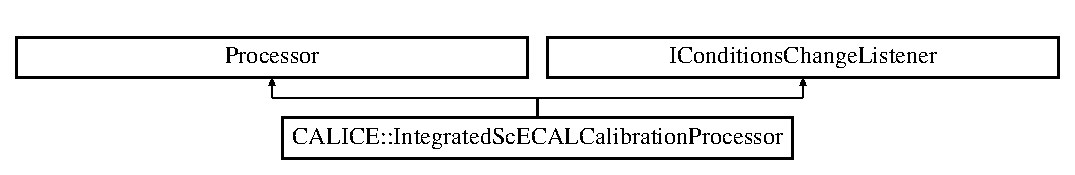
\includegraphics[height=1.904762cm]{classCALICE_1_1IntegratedScECALCalibrationProcessor}
\end{center}
\end{figure}
\subsection*{Public Member Functions}
\begin{DoxyCompactItemize}
\item 
{\bf Integrated\-Sc\-E\-C\-A\-L\-Calibration\-Processor} $\ast$ {\bfseries new\-Processor} ()\label{classCALICE_1_1IntegratedScECALCalibrationProcessor_a80d8d7e14fa1e0838dc6b95f087a2705}

\item 
virtual void {\bfseries init} ()\label{classCALICE_1_1IntegratedScECALCalibrationProcessor_aa1eab42e9957dfcf3eb2c6c6fb91a13f}

\item 
virtual void {\bfseries process\-Run\-Header} (L\-C\-Run\-Header $\ast$run)\label{classCALICE_1_1IntegratedScECALCalibrationProcessor_acdffaa1d6fc44f196e4cb7a70cd02fcc}

\item 
virtual void {\bfseries process\-Event} (lcio\-::\-L\-C\-Event $\ast$evt)\label{classCALICE_1_1IntegratedScECALCalibrationProcessor_a146cb14128685b8841aac56473c77cad}

\item 
virtual void {\bfseries conditions\-Changed} (L\-C\-Collection $\ast$col)\label{classCALICE_1_1IntegratedScECALCalibrationProcessor_a50ff3bbb91c9e9f16882507b10b4edf7}

\item 
virtual void {\bfseries end} ()\label{classCALICE_1_1IntegratedScECALCalibrationProcessor_a4d3b93362d14bec35af499d016a21cd2}

\end{DoxyCompactItemize}
\subsection*{Protected Attributes}
\begin{DoxyCompactItemize}
\item 
int {\bfseries \-\_\-list\-Read\-Counter}\label{classCALICE_1_1IntegratedScECALCalibrationProcessor_aa242bf8b17ea06ba0c3a29651ccf03c7}

\item 
std\-::map$<$ long64, float $>$ {\bfseries \-\_\-templist}\label{classCALICE_1_1IntegratedScECALCalibrationProcessor_ad97e4e34867d7fa28a1eb07ea6220af7}

\item 
std\-::map$<$ int, map$<$ long64, \\*
float $>$ $>$ {\bfseries \-\_\-temp\-Order}\label{classCALICE_1_1IntegratedScECALCalibrationProcessor_af562fe94a00b1e2a214d23dfc6046082}

\item 
int {\bfseries \-\_\-data\-Year}\label{classCALICE_1_1IntegratedScECALCalibrationProcessor_adabbfd2f9d989e06a31acf5df9404018}

\item 
bool {\bfseries \-\_\-for\-M\-I\-P\-Calibration}\label{classCALICE_1_1IntegratedScECALCalibrationProcessor_a5954f01e887988d58dfb4d0c449f671a}

\item 
bool {\bfseries \-\_\-tempcorrgain\-On}\label{classCALICE_1_1IntegratedScECALCalibrationProcessor_a5b2f5d0be9d2564c1f26136dc19c2812}

\item 
bool {\bfseries \-\_\-tempcorrmip\-On}\label{classCALICE_1_1IntegratedScECALCalibrationProcessor_a26685b20a13b1ec113ed710f5066f3da}

\item 
std\-::vector$<$ float $>$ {\bfseries \-\_\-tempcorr\-\_\-gain}\label{classCALICE_1_1IntegratedScECALCalibrationProcessor_a6bea424148f94a17f5b1bcaa9560b4f1}

\item 
std\-::vector$<$ float $>$ {\bfseries \-\_\-tempcorr\-\_\-mip}\label{classCALICE_1_1IntegratedScECALCalibrationProcessor_a96a833648299a5ac4ab5e961e5ce5425}

\item 
std\-::vector$<$ int $>$ {\bfseries \-\_\-offset\-Time\-Stamp}\label{classCALICE_1_1IntegratedScECALCalibrationProcessor_a8156f18fe252c98f723382db01ce9d80}

\item 
std\-::vector$<$ int $>$ {\bfseries \-\_\-ondotori2stamp}\label{classCALICE_1_1IntegratedScECALCalibrationProcessor_a8a2a540275a5de1c440ea6389f549868}

\item 
int {\bfseries \-\_\-nnoisy}\label{classCALICE_1_1IntegratedScECALCalibrationProcessor_a9ce2884633802f471e62c13483ced0a2}

\item 
int {\bfseries \-\_\-noisychan\-Layer} [Sc\-E\-C\-A\-L\-\_\-\-N\-L\-A\-Y\-E\-R\-S $\ast$Sc\-E\-C\-A\-L\-\_\-\-N\-S\-T\-R\-I\-P\-S]\label{classCALICE_1_1IntegratedScECALCalibrationProcessor_aadbc356c230573212c8c1e9f9f3f41cc}

\item 
int {\bfseries \-\_\-noisychan\-Strip} [Sc\-E\-C\-A\-L\-\_\-\-N\-L\-A\-Y\-E\-R\-S $\ast$Sc\-E\-C\-A\-L\-\_\-\-N\-S\-T\-R\-I\-P\-S]\label{classCALICE_1_1IntegratedScECALCalibrationProcessor_ad5fb35024421a55936030f4f7469fbd7}

\item 
float {\bfseries \-\_\-eff\-Npix}\label{classCALICE_1_1IntegratedScECALCalibrationProcessor_afede1e6bc146049a6553c9801fe839dd}

\item 
std\-::string {\bfseries \-\_\-input\-Col\-Name}\label{classCALICE_1_1IntegratedScECALCalibrationProcessor_ac42a0277e9b4dc421591e8d3df6e76c4}

\item 
std\-::string {\bfseries \-\_\-output\-Col\-Name}\label{classCALICE_1_1IntegratedScECALCalibrationProcessor_afc10b206d4c70c3254ee8db9c7983e8f}

\item 
bool {\bfseries \-\_\-zero\-Suppression}\label{classCALICE_1_1IntegratedScECALCalibrationProcessor_a3bc7d6f1828510d0a9588f23f8c201eb}

\item 
float {\bfseries \-\_\-significance\-Cut}\label{classCALICE_1_1IntegratedScECALCalibrationProcessor_a30185444af319ee6da502b64817e82f6}

\item 
bool {\bfseries \-\_\-skip\-Pedestals}\label{classCALICE_1_1IntegratedScECALCalibrationProcessor_a78af7130e141695755c6e3448ca73283}

\item 
int {\bfseries \-\_\-min\-Ped\-Number}\label{classCALICE_1_1IntegratedScECALCalibrationProcessor_a1a2f99e38ea563324ffbeff1f342848b}

\item 
int {\bfseries \-\_\-ped\-Counter}\label{classCALICE_1_1IntegratedScECALCalibrationProcessor_ad2e2dfb9ed38a0fb477e49422affe3db}

\item 
bool {\bfseries \-\_\-pedestal\-Subtraction}\label{classCALICE_1_1IntegratedScECALCalibrationProcessor_abb28167c1947ecb2fa63693acb5088a7}

\item 
float {\bfseries \-\_\-mip\-Cut}\label{classCALICE_1_1IntegratedScECALCalibrationProcessor_a9aa1b3b1267dfb7d9f93779f365171e2}

\item 
unsigned long {\bfseries \-\_\-hit\-Counter}\label{classCALICE_1_1IntegratedScECALCalibrationProcessor_ae7f0adccf76ae6c22c6e5f748d8c9899}

\item 
unsigned long {\bfseries \-\_\-invalid\-M\-I\-P\-Counter}\label{classCALICE_1_1IntegratedScECALCalibrationProcessor_a32073bf9073c927af764495b53a0dc97}

\item 
unsigned long {\bfseries \-\_\-invalid\-Saturation\-Correction\-Counter}\label{classCALICE_1_1IntegratedScECALCalibrationProcessor_a99fd828abc1342d785aaf6a68d78a94b}

\item 
unsigned long {\bfseries \-\_\-saturation\-Counter}\label{classCALICE_1_1IntegratedScECALCalibrationProcessor_a2d2db54c3e186e77f0f3a02ce8bf2254}

\item 
unsigned long {\bfseries \-\_\-event\-Counter}\label{classCALICE_1_1IntegratedScECALCalibrationProcessor_a934d12f20ce5258bd13386757d521b0f}

\item 
std\-::vector$<$ float $>$ {\bfseries \-\_\-gain\-Lim}\label{classCALICE_1_1IntegratedScECALCalibrationProcessor_a11b496da02ff2a2fe2b96fdd4b4dde44}

\item 
std\-::vector$<$ float $>$ {\bfseries \-\_\-gain\-Err\-Lim}\label{classCALICE_1_1IntegratedScECALCalibrationProcessor_a0eda6f27afb85a12b296cbc9340d2459}

\item 
std\-::vector$<$ float $>$ {\bfseries \-\_\-uniform\-Gain\-Slope}\label{classCALICE_1_1IntegratedScECALCalibrationProcessor_a42ae562273b47e5733ea2d3c2473a68c}

\item 
std\-::map$<$ unsigned, unsigned $>$ {\bfseries \-\_\-invalid\-M\-I\-P\-Calibrations}\label{classCALICE_1_1IntegratedScECALCalibrationProcessor_a2699b026f88dd2671d112a050ba71b03}

\item 
std\-::map$<$ unsigned, unsigned $>$ {\bfseries \-\_\-invalid\-Saturation\-Corrections}\label{classCALICE_1_1IntegratedScECALCalibrationProcessor_a14bbf47f43ebe5e33683b1d47ef4b45d}

\item 
std\-::map$<$ unsigned, unsigned $>$ {\bfseries \-\_\-saturations}\label{classCALICE_1_1IntegratedScECALCalibrationProcessor_ac6a2ff79eb4fab82925e36edae58d22a}

\item 
double {\bfseries \-\_\-ped\-Sum} [Sc\-E\-C\-A\-L\-\_\-\-N\-L\-A\-Y\-E\-R\-S][Sc\-E\-C\-A\-L\-\_\-\-N\-S\-T\-R\-I\-P\-S]\label{classCALICE_1_1IntegratedScECALCalibrationProcessor_a09e83cb1d46116f9bddd9f5f8259758e}

\item 
double {\bfseries \-\_\-ped\-Sum\-Square} [Sc\-E\-C\-A\-L\-\_\-\-N\-L\-A\-Y\-E\-R\-S][Sc\-E\-C\-A\-L\-\_\-\-N\-S\-T\-R\-I\-P\-S]\label{classCALICE_1_1IntegratedScECALCalibrationProcessor_a22ca651c37cdca77e318183ac28d124b}

\item 
unsigned {\bfseries \-\_\-ped\-Num} [Sc\-E\-C\-A\-L\-\_\-\-N\-L\-A\-Y\-E\-R\-S][Sc\-E\-C\-A\-L\-\_\-\-N\-S\-T\-R\-I\-P\-S]\label{classCALICE_1_1IntegratedScECALCalibrationProcessor_adaa3b48097f3a56add3a9dbaaac9d288}

\item 
float {\bfseries \-\_\-ped} [Sc\-E\-C\-A\-L\-\_\-\-N\-L\-A\-Y\-E\-R\-S][Sc\-E\-C\-A\-L\-\_\-\-N\-S\-T\-R\-I\-P\-S]\label{classCALICE_1_1IntegratedScECALCalibrationProcessor_a9d86971a1ebd696affd4df5702f84d93}

\item 
float {\bfseries \-\_\-ped\-Error} [Sc\-E\-C\-A\-L\-\_\-\-N\-L\-A\-Y\-E\-R\-S][Sc\-E\-C\-A\-L\-\_\-\-N\-S\-T\-R\-I\-P\-S]\label{classCALICE_1_1IntegratedScECALCalibrationProcessor_ada246c89a647be0ab4b33365e461a0c2}

\item 
double {\bfseries \-\_\-mipcalibconst} [Sc\-E\-C\-A\-L\-\_\-\-N\-L\-A\-Y\-E\-R\-S][Sc\-E\-C\-A\-L\-\_\-\-N\-S\-T\-R\-I\-P\-S]\label{classCALICE_1_1IntegratedScECALCalibrationProcessor_acf61619680c7df4ffab1cf1a759b6f92}

\item 
double {\bfseries \-\_\-mipcalibconst\-\_\-err} [Sc\-E\-C\-A\-L\-\_\-\-N\-L\-A\-Y\-E\-R\-S][Sc\-E\-C\-A\-L\-\_\-\-N\-S\-T\-R\-I\-P\-S]\label{classCALICE_1_1IntegratedScECALCalibrationProcessor_a1fe73446252d0efa3e77523e2c645b1a}

\item 
double {\bfseries \-\_\-mip\-Slope} [Sc\-E\-C\-A\-L\-\_\-\-N\-L\-A\-Y\-E\-R\-S][Sc\-E\-C\-A\-L\-\_\-\-N\-S\-T\-R\-I\-P\-S]\label{classCALICE_1_1IntegratedScECALCalibrationProcessor_a51de70a9fb886693481b7c7e3173fed1}

\item 
double {\bfseries \-\_\-mip\-Slope\-Err} [Sc\-E\-C\-A\-L\-\_\-\-N\-L\-A\-Y\-E\-R\-S][Sc\-E\-C\-A\-L\-\_\-\-N\-S\-T\-R\-I\-P\-S]\label{classCALICE_1_1IntegratedScECALCalibrationProcessor_a883ef441c0a3098f7319e1e8d48aada2}

\item 
double {\bfseries \-\_\-mip\-Set\-Temp} [Sc\-E\-C\-A\-L\-\_\-\-N\-L\-A\-Y\-E\-R\-S][Sc\-E\-C\-A\-L\-\_\-\-N\-S\-T\-R\-I\-P\-S]\label{classCALICE_1_1IntegratedScECALCalibrationProcessor_a256c3d9ae521ccef87b79c161616be65}

\item 
double {\bfseries \-\_\-gaincalibconst} [Sc\-E\-C\-A\-L\-\_\-\-N\-L\-A\-Y\-E\-R\-S][Sc\-E\-C\-A\-L\-\_\-\-N\-S\-T\-R\-I\-P\-S]\label{classCALICE_1_1IntegratedScECALCalibrationProcessor_ac01bc7902f8f262fa3590f0facb31ebc}

\item 
double {\bfseries \-\_\-gaincalibconst\-\_\-err} [Sc\-E\-C\-A\-L\-\_\-\-N\-L\-A\-Y\-E\-R\-S][Sc\-E\-C\-A\-L\-\_\-\-N\-S\-T\-R\-I\-P\-S]\label{classCALICE_1_1IntegratedScECALCalibrationProcessor_ad6651fc69410049bdde46bfda31192e3}

\item 
double {\bfseries \-\_\-gain\-Slope} [Sc\-E\-C\-A\-L\-\_\-\-N\-L\-A\-Y\-E\-R\-S][Sc\-E\-C\-A\-L\-\_\-\-N\-S\-T\-R\-I\-P\-S]\label{classCALICE_1_1IntegratedScECALCalibrationProcessor_a0c09c5acb333c533ac0dc9d5081c6076}

\item 
double {\bfseries \-\_\-gain\-Slope\-Err} [Sc\-E\-C\-A\-L\-\_\-\-N\-L\-A\-Y\-E\-R\-S][Sc\-E\-C\-A\-L\-\_\-\-N\-S\-T\-R\-I\-P\-S]\label{classCALICE_1_1IntegratedScECALCalibrationProcessor_ad9122fb35196a1e8c128bc810dd73f48}

\item 
double {\bfseries \-\_\-gain\-Set\-Temp} [Sc\-E\-C\-A\-L\-\_\-\-N\-L\-A\-Y\-E\-R\-S][Sc\-E\-C\-A\-L\-\_\-\-N\-S\-T\-R\-I\-P\-S]\label{classCALICE_1_1IntegratedScECALCalibrationProcessor_a0d302f9a7fe000202b8e2b3315e37a42}

\item 
double {\bfseries \-\_\-intercalibconst} [Sc\-E\-C\-A\-L\-\_\-\-N\-L\-A\-Y\-E\-R\-S][Sc\-E\-C\-A\-L\-\_\-\-N\-S\-T\-R\-I\-P\-S]\label{classCALICE_1_1IntegratedScECALCalibrationProcessor_a19843391c2f2d492ee8d07cf560d61b3}

\item 
double {\bfseries \-\_\-intercalibconst\-\_\-err} [Sc\-E\-C\-A\-L\-\_\-\-N\-L\-A\-Y\-E\-R\-S][Sc\-E\-C\-A\-L\-\_\-\-N\-S\-T\-R\-I\-P\-S]\label{classCALICE_1_1IntegratedScECALCalibrationProcessor_a447fee3ab3e691f7753e77849a3f5156}

\item 
std\-::string {\bfseries \-\_\-\-Sc\-E\-C\-A\-L\-M\-I\-P\-Col\-Name}\label{classCALICE_1_1IntegratedScECALCalibrationProcessor_a23fa64acf0c4c56a27cd218e45a72a95}

\item 
L\-C\-Collection $\ast$ {\bfseries \-\_\-\-Sc\-E\-C\-A\-L\-M\-I\-P\-Col}\label{classCALICE_1_1IntegratedScECALCalibrationProcessor_af9da8b814eec1d7428a50f752826816b}

\item 
bool {\bfseries \-\_\-\-M\-I\-P\-Constant\-Changed}\label{classCALICE_1_1IntegratedScECALCalibrationProcessor_a7adcc04792d1e9c91be42fffb9650ecb}

\item 
std\-::string {\bfseries \-\_\-\-Sc\-E\-C\-A\-L\-Int\-Calib\-Col\-Name}\label{classCALICE_1_1IntegratedScECALCalibrationProcessor_a06cf578e8d2e90e83423c4cda9212719}

\item 
L\-C\-Collection $\ast$ {\bfseries \-\_\-\-Sc\-E\-C\-A\-L\-Int\-Calib\-Col}\label{classCALICE_1_1IntegratedScECALCalibrationProcessor_a0ff44ca5a38c2b4b95b6f66e532c0f0f}

\item 
bool {\bfseries \-\_\-\-Int\-Calib\-Const\-Changed}\label{classCALICE_1_1IntegratedScECALCalibrationProcessor_a79ad2dea374a18735ecf63568815738e}

\item 
std\-::string {\bfseries \-\_\-\-Sc\-E\-C\-A\-L\-Gain\-Col\-Name}\label{classCALICE_1_1IntegratedScECALCalibrationProcessor_a35226bdbae7c441b3537037d5100d27c}

\item 
L\-C\-Collection $\ast$ {\bfseries \-\_\-\-Sc\-E\-C\-A\-L\-Gain\-Col}\label{classCALICE_1_1IntegratedScECALCalibrationProcessor_aafd6b24dd5fbfcf0abeeb5c887faa07a}

\item 
bool {\bfseries \-\_\-\-Gain\-Const\-Changed}\label{classCALICE_1_1IntegratedScECALCalibrationProcessor_ab7f94c6e651268e510283572be35fb5f}

\item 
std\-::string {\bfseries \-\_\-\-Sc\-E\-C\-A\-L\-Temperature\-Col\-Name}\label{classCALICE_1_1IntegratedScECALCalibrationProcessor_a3965c116379097f3dd18979b694d23e4}

\item 
L\-C\-Collection $\ast$ {\bfseries \-\_\-\-Sc\-E\-C\-A\-L\-Temperature\-Col}\label{classCALICE_1_1IntegratedScECALCalibrationProcessor_a48a9a574f0f7377f9e8dc16a99b7a45a}

\item 
bool {\bfseries \-\_\-\-Temperature\-Changed}\label{classCALICE_1_1IntegratedScECALCalibrationProcessor_ab2e5c24c94b27fd94a70bebb8a071aea}

\item 
std\-::string {\bfseries \-\_\-\-Sc\-E\-C\-A\-L\-Noisy\-Channel\-Col\-Name}\label{classCALICE_1_1IntegratedScECALCalibrationProcessor_a234c5e12f557aebf5752f95e53ca68a7}

\item 
L\-C\-Collection $\ast$ {\bfseries \-\_\-\-Sc\-E\-C\-A\-L\-Noisy\-Channel\-Col}\label{classCALICE_1_1IntegratedScECALCalibrationProcessor_aa04542cfddd279b2c0254916e9d830a2}

\item 
bool {\bfseries \-\_\-\-Noisy\-Channel\-Changed}\label{classCALICE_1_1IntegratedScECALCalibrationProcessor_a920d09ab58c742d08d16599ab661eae2}

\end{DoxyCompactItemize}


\subsection{Detailed Description}


Definition at line 47 of file Integrated\-Sc\-E\-C\-A\-L\-Calibration\-Processor.\-hh.



The documentation for this class was generated from the following files\-:\begin{DoxyCompactItemize}
\item 
Integrated\-Sc\-E\-C\-A\-L\-Calibration\-Processor.\-hh\item 
Integrated\-Sc\-E\-C\-A\-L\-Calibration\-Processor.\-cc\end{DoxyCompactItemize}

\section{histmgr\-:\-:Key\-\_\-t Class Reference}
\label{classhistmgr_1_1Key__t}\index{histmgr\-::\-Key\-\_\-t@{histmgr\-::\-Key\-\_\-t}}


A string key which will get a numeric identifier.  




{\ttfamily \#include $<$Key\-\_\-t.\-hh$>$}

\subsection*{Public Member Functions}
\begin{DoxyCompactItemize}
\item 
{\bfseries Key\-\_\-t} (const std\-::string \&key\-\_\-name)\label{classhistmgr_1_1Key__t_afce4e8a705f0f1a672177ba34000df14}

\item 
std\-::string \& {\bfseries name\-Storage} ()\label{classhistmgr_1_1Key__t_ae94241f0863c94f48c8de3526b21a5ef}

\item 
const std\-::string \& {\bfseries name} () const \label{classhistmgr_1_1Key__t_afb953f811ee1274e7d8c96800760dcd1}

\item 
unsigned int {\bfseries id} () const \label{classhistmgr_1_1Key__t_a46ee73330ff61b8d100edad91614a6eb}

\item 
bool {\bfseries is\-Set} () const \label{classhistmgr_1_1Key__t_aa09f615fc00440b4a56902a3d3076d61}

\end{DoxyCompactItemize}
\subsection*{Static Public Member Functions}
\begin{DoxyCompactItemize}
\item 
static unsigned int {\bfseries invalid\-Key} ()\label{classhistmgr_1_1Key__t_a3f76a8ecb4e1226f9e598199d0c194a0}

\end{DoxyCompactItemize}
\subsection*{Protected Member Functions}
\begin{DoxyCompactItemize}
\item 
void {\bfseries cache} (unsigned int id) const \label{classhistmgr_1_1Key__t_a27779ea465a99d049b4e7f388b4ab3e5}

\end{DoxyCompactItemize}
\subsection*{Private Attributes}
\begin{DoxyCompactItemize}
\item 
std\-::string {\bfseries \-\_\-name}\label{classhistmgr_1_1Key__t_a3ef2f7aa7639d24c9c94389a7e08cc52}

\item 
unsigned int {\bfseries \-\_\-id}\label{classhistmgr_1_1Key__t_a6bd85027f8ed355208f46dbbfbc314df}

\end{DoxyCompactItemize}
\subsection*{Friends}
\begin{DoxyCompactItemize}
\item 
{\footnotesize template$<$typename T $>$ }\\class {\bfseries Key\-Map\-\_\-t}\label{classhistmgr_1_1Key__t_ac6e344ee1199919f6cdaa7f11ab5ac9d}

\item 
class {\bfseries Key\-Map\-Base\-\_\-t}\label{classhistmgr_1_1Key__t_a9575e83b8b317dbc46a599683d98e086}

\end{DoxyCompactItemize}


\subsection{Detailed Description}
A string key which will get a numeric identifier. 

The primary key is the name. To prevent numerours string lookups, a numeric identifier is assigned to each string key. The numeric identifier is declared mutable. It will be set nevertheless of the const-\/ness of the class. 

Definition at line 16 of file Key\-\_\-t.\-hh.



The documentation for this class was generated from the following file\-:\begin{DoxyCompactItemize}
\item 
Key\-\_\-t.\-hh\end{DoxyCompactItemize}

\section{histmgr\-:\-:Key\-Map\-\_\-t$<$ T $>$ Class Template Reference}
\label{classhistmgr_1_1KeyMap__t}\index{histmgr\-::\-Key\-Map\-\_\-t$<$ T $>$@{histmgr\-::\-Key\-Map\-\_\-t$<$ T $>$}}


List of elements (Key\-Map).  




{\ttfamily \#include $<$Key\-Map\-\_\-t.\-hh$>$}

Inheritance diagram for histmgr\-:\-:Key\-Map\-\_\-t$<$ T $>$\-:\begin{figure}[H]
\begin{center}
\leavevmode
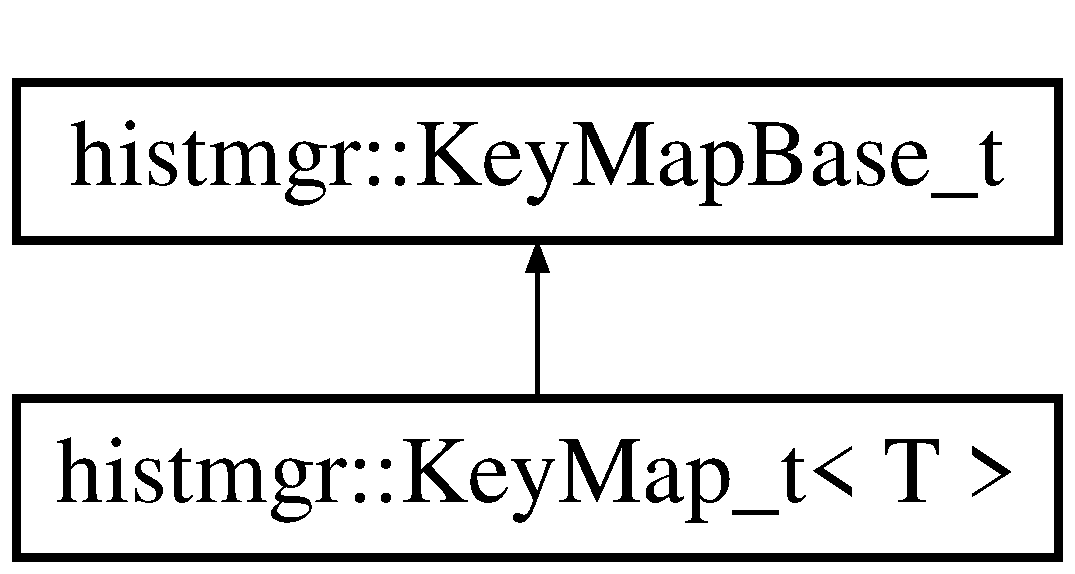
\includegraphics[height=2.000000cm]{classhistmgr_1_1KeyMap__t}
\end{center}
\end{figure}
\subsection*{Public Types}
\begin{DoxyCompactItemize}
\item 
typedef {\bf Key\-Map\-Iterator\-\_\-t}\\*
$<$ \-\_\-\-Map\-Elm\-\_\-t\-\_\- $>$ {\bfseries iterator}\label{classhistmgr_1_1KeyMap__t_a36f08060446052445a89c1ab95a93c49}

\item 
typedef {\bf Key\-Map\-Const\-Iterator\-\_\-t}\\*
$<$ \-\_\-\-Map\-Elm\-\_\-t\-\_\- $>$ {\bfseries const\-\_\-iterator}\label{classhistmgr_1_1KeyMap__t_ae16884e84c02259cff1074864660d304}

\end{DoxyCompactItemize}
\subsection*{Public Member Functions}
\begin{DoxyCompactItemize}
\item 
bool {\bf has\-Key} (const {\bf Key\-\_\-t} \&a\-\_\-key) const \label{classhistmgr_1_1KeyMap__t_a6a1c898e2de5448de3514e4691c67b8a}

\begin{DoxyCompactList}\small\item\em Check whether an element exist already for the given key. \end{DoxyCompactList}\item 
void {\bf assign} (const {\bf Key\-\_\-t} \&a\-\_\-key, const \-\_\-\-Map\-Elm\-\_\-t\-\_\- \&elm)
\begin{DoxyCompactList}\small\item\em Assign an element to the given key. \end{DoxyCompactList}\item 
\-\_\-\-Map\-Elm\-\_\-t\-\_\- \& {\bf operator[$\,$]} (const {\bf Key\-\_\-t} \&a\-\_\-key)
\begin{DoxyCompactList}\small\item\em Get the element assigned to the given key. \end{DoxyCompactList}\item 
const \-\_\-\-Map\-Elm\-\_\-t\-\_\- \& {\bf operator[$\,$]} (const {\bf Key\-\_\-t} \&a\-\_\-key) const 
\begin{DoxyCompactList}\small\item\em Get the element assigned to the given key (read only access). \end{DoxyCompactList}\item 
{\bf iterator} {\bfseries begin} ()\label{classhistmgr_1_1KeyMap__t_ad8f934b50be1b263b4151ee1eda1d91c}

\item 
{\bf iterator} {\bfseries end} ()\label{classhistmgr_1_1KeyMap__t_a04b15116bdfb56e764d4bea63c1b4933}

\item 
{\bf const\-\_\-iterator} {\bfseries begin} () const \label{classhistmgr_1_1KeyMap__t_a68aad70b6250caa7278cdfff4a77bdaa}

\item 
{\bf const\-\_\-iterator} {\bfseries end} () const \label{classhistmgr_1_1KeyMap__t_a7ffe8a8499fda4ec1a265e4c4970c012}

\end{DoxyCompactItemize}
\subsection*{Private Attributes}
\begin{DoxyCompactItemize}
\item 
std\-::vector$<$ \-\_\-\-Map\-Elm\-\_\-t\-\_\- $>$ {\bfseries \-\_\-elm\-List}\label{classhistmgr_1_1KeyMap__t_a16a7214a6a6f4798b9a20f1e5efa625c}

\end{DoxyCompactItemize}
\subsection*{Friends}
\begin{DoxyCompactItemize}
\item 
class {\bfseries Hist\-Mgr}\label{classhistmgr_1_1KeyMap__t_a3cc85db784d7651390e41024125eb3a0}

\end{DoxyCompactItemize}
\subsection*{Additional Inherited Members}


\subsection{Detailed Description}
\subsubsection*{template$<$typename T$>$class histmgr\-::\-Key\-Map\-\_\-t$<$ T $>$}

List of elements (Key\-Map). 

The elements are identified by their names. A contrinuous serial number is assigned to each element. The serial number can be used to quickly access the histograms 

Definition at line 8 of file Key\-\_\-t.\-hh.



\subsection{Member Function Documentation}
\index{histmgr\-::\-Key\-Map\-\_\-t@{histmgr\-::\-Key\-Map\-\_\-t}!assign@{assign}}
\index{assign@{assign}!histmgr::KeyMap_t@{histmgr\-::\-Key\-Map\-\_\-t}}
\subsubsection[{assign}]{\setlength{\rightskip}{0pt plus 5cm}template$<$typename T$>$ void {\bf histmgr\-::\-Key\-Map\-\_\-t}$<$ T $>$\-::assign (
\begin{DoxyParamCaption}
\item[{const {\bf Key\-\_\-t} \&}]{a\-\_\-key, }
\item[{const \-\_\-\-Map\-Elm\-\_\-t\-\_\- \&}]{elm}
\end{DoxyParamCaption}
)\hspace{0.3cm}{\ttfamily [inline]}}\label{classhistmgr_1_1KeyMap__t_ae3cf5c9453199e37c02a6cf3f9361fbc}


Assign an element to the given key. 


\begin{DoxyParams}{Parameters}
{\em a\-\_\-key} & the key to which an element should be assigned. \\
\hline
{\em elm} & the element. If an element is already assigned to the key, then the old element is deleted. \\
\hline
\end{DoxyParams}


Definition at line 221 of file Key\-Map\-\_\-t.\-hh.



Referenced by histmgr\-::\-Hist\-Mgr\-::get\-Or\-Createhistogram\-Group().

\index{histmgr\-::\-Key\-Map\-\_\-t@{histmgr\-::\-Key\-Map\-\_\-t}!operator[$\,$]@{operator[]}}
\index{operator[$\,$]@{operator[]}!histmgr::KeyMap_t@{histmgr\-::\-Key\-Map\-\_\-t}}
\subsubsection[{operator[]}]{\setlength{\rightskip}{0pt plus 5cm}template$<$typename T$>$ \-\_\-\-Map\-Elm\-\_\-t\-\_\-\& {\bf histmgr\-::\-Key\-Map\-\_\-t}$<$ T $>$\-::operator[$\,$] (
\begin{DoxyParamCaption}
\item[{const {\bf Key\-\_\-t} \&}]{a\-\_\-key}
\end{DoxyParamCaption}
)\hspace{0.3cm}{\ttfamily [inline]}}\label{classhistmgr_1_1KeyMap__t_a9296088594f214a57181ade2dbb4c341}


Get the element assigned to the given key. 


\begin{DoxyParams}{Parameters}
{\em a\-\_\-key} & the key of the element. \\
\hline
\end{DoxyParams}


Definition at line 236 of file Key\-Map\-\_\-t.\-hh.

\index{histmgr\-::\-Key\-Map\-\_\-t@{histmgr\-::\-Key\-Map\-\_\-t}!operator[$\,$]@{operator[]}}
\index{operator[$\,$]@{operator[]}!histmgr::KeyMap_t@{histmgr\-::\-Key\-Map\-\_\-t}}
\subsubsection[{operator[]}]{\setlength{\rightskip}{0pt plus 5cm}template$<$typename T$>$ const \-\_\-\-Map\-Elm\-\_\-t\-\_\-\& {\bf histmgr\-::\-Key\-Map\-\_\-t}$<$ T $>$\-::operator[$\,$] (
\begin{DoxyParamCaption}
\item[{const {\bf Key\-\_\-t} \&}]{a\-\_\-key}
\end{DoxyParamCaption}
) const\hspace{0.3cm}{\ttfamily [inline]}}\label{classhistmgr_1_1KeyMap__t_a730444af2fc5027c6a8ee4ef8cddf7c6}


Get the element assigned to the given key (read only access). 


\begin{DoxyParams}{Parameters}
{\em a\-\_\-key} & the key of the element. \\
\hline
\end{DoxyParams}


Definition at line 247 of file Key\-Map\-\_\-t.\-hh.



The documentation for this class was generated from the following files\-:\begin{DoxyCompactItemize}
\item 
Key\-\_\-t.\-hh\item 
Key\-Map\-\_\-t.\-hh\end{DoxyCompactItemize}

\section{histmgr\-:\-:Key\-Map\-Base\-\_\-t Class Reference}
\label{classhistmgr_1_1KeyMapBase__t}\index{histmgr\-::\-Key\-Map\-Base\-\_\-t@{histmgr\-::\-Key\-Map\-Base\-\_\-t}}


Base class of the element list which only manages the name mapping.  




{\ttfamily \#include $<$Key\-Map\-\_\-t.\-hh$>$}

Inheritance diagram for histmgr\-:\-:Key\-Map\-Base\-\_\-t\-:\begin{figure}[H]
\begin{center}
\leavevmode
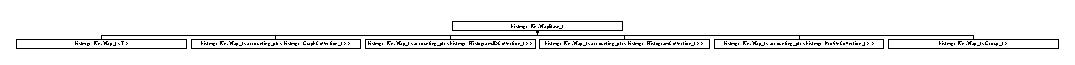
\includegraphics[height=0.425209cm]{classhistmgr_1_1KeyMapBase__t}
\end{center}
\end{figure}
\subsection*{Public Types}
\begin{DoxyCompactItemize}
\item 
typedef std\-::map$<$ std\-::string, \\*
unsigned int $>$ {\bfseries Name\-Map\-\_\-t}\label{classhistmgr_1_1KeyMapBase__t_ae49c6a47e8e2391af4a57a3dc1f40020}

\end{DoxyCompactItemize}
\subsection*{Public Member Functions}
\begin{DoxyCompactItemize}
\item 
Name\-Map\-\_\-t\-::const\-\_\-iterator {\bfseries name\-List\-Begin} () const \label{classhistmgr_1_1KeyMapBase__t_af1bc65af4564e7cd74c6ab25b35ca9e5}

\item 
Name\-Map\-\_\-t\-::const\-\_\-iterator {\bfseries name\-List\-End} () const \label{classhistmgr_1_1KeyMapBase__t_aac7ea5403cabbabff2a01dc108072f1f}

\item 
bool {\bfseries empty} () const \label{classhistmgr_1_1KeyMapBase__t_a63938a3f927f441c92a91467eee12fa4}

\item 
unsigned int {\bfseries size} () const \label{classhistmgr_1_1KeyMapBase__t_abe4ee7508376462845afcfe84ce92672}

\end{DoxyCompactItemize}
\subsection*{Static Public Member Functions}
\begin{DoxyCompactItemize}
\item 
static {\bf Key\-\_\-t} {\bfseries create\-Key} (Name\-Map\-\_\-t\-::const\-\_\-iterator \&iter)\label{classhistmgr_1_1KeyMapBase__t_a0abfc2a6b98414d55e92a0c9c69b4b29}

\end{DoxyCompactItemize}
\subsection*{Protected Member Functions}
\begin{DoxyCompactItemize}
\item 
bool {\bf \-\_\-has\-Key} (const {\bf Key\-\_\-t} \&a\-\_\-key) const \label{classhistmgr_1_1KeyMapBase__t_aed1d4e8444789c2f0089bec2b68a091b}

\begin{DoxyCompactList}\small\item\em Check whether an element exist already for the given key. \end{DoxyCompactList}\item 
bool {\bfseries \-\_\-insert\-New} (const {\bf Key\-\_\-t} \&a\-\_\-key, unsigned int next\-\_\-element)\label{classhistmgr_1_1KeyMapBase__t_a8c886c4d400a0549978b170ddd846d1e}

\item 
bool {\bfseries \-\_\-set\-Index\-Cache} (const {\bf Key\-\_\-t} \&a\-\_\-key)\label{classhistmgr_1_1KeyMapBase__t_a51614c13e31ea6616cefd41580c92288}

\end{DoxyCompactItemize}
\subsection*{Protected Attributes}
\begin{DoxyCompactItemize}
\item 
Name\-Map\-\_\-t {\bfseries \-\_\-id\-List}\label{classhistmgr_1_1KeyMapBase__t_a759b7cd45f2bff8c5c5c83954c3f1295}

\end{DoxyCompactItemize}
\subsection*{Friends}
\begin{DoxyCompactItemize}
\item 
class {\bfseries Hist\-Mgr}\label{classhistmgr_1_1KeyMapBase__t_a3cc85db784d7651390e41024125eb3a0}

\end{DoxyCompactItemize}


\subsection{Detailed Description}
Base class of the element list which only manages the name mapping. 

Definition at line 22 of file Key\-Map\-\_\-t.\-hh.



The documentation for this class was generated from the following file\-:\begin{DoxyCompactItemize}
\item 
Key\-Map\-\_\-t.\-hh\end{DoxyCompactItemize}

\section{histmgr\-:\-:Key\-Map\-Const\-Iterator\-\_\-t$<$ \-\_\-\-Map\-\_\-t\-\_\- $>$ Class Template Reference}
\label{classhistmgr_1_1KeyMapConstIterator__t}\index{histmgr\-::\-Key\-Map\-Const\-Iterator\-\_\-t$<$ \-\_\-\-Map\-\_\-t\-\_\- $>$@{histmgr\-::\-Key\-Map\-Const\-Iterator\-\_\-t$<$ \-\_\-\-Map\-\_\-t\-\_\- $>$}}


Const Iterator for the Key\-Map.  




{\ttfamily \#include $<$Key\-Map\-\_\-t.\-hh$>$}

\subsection*{Public Member Functions}
\begin{DoxyCompactItemize}
\item 
{\bf Key\-Map\-Const\-Iterator\-\_\-t} \& {\bfseries operator++} (int)\label{classhistmgr_1_1KeyMapConstIterator__t_a836ba25c49adada842fbae460c128324}

\item 
const \-\_\-\-Map\-\_\-t\-\_\- \& {\bfseries operator$\ast$} () const \label{classhistmgr_1_1KeyMapConstIterator__t_ab5b2ed2dd09f955fac73a81ea946a279}

\item 
bool {\bfseries operator!=} (const {\bf Key\-Map\-Const\-Iterator\-\_\-t} \&a)\label{classhistmgr_1_1KeyMapConstIterator__t_a6287d9b0a5a0416e7fb7148b4e7c8d50}

\item 
bool {\bfseries operator==} (const {\bf Key\-Map\-Const\-Iterator\-\_\-t} \&a)\label{classhistmgr_1_1KeyMapConstIterator__t_a1d8772a655ce9206fc4ca55ec1180d10}

\item 
const std\-::string \& {\bfseries name} () const \label{classhistmgr_1_1KeyMapConstIterator__t_a177a0274749f6e1886bc635f710ee8ab}

\end{DoxyCompactItemize}
\subsection*{Data Fields}
\begin{DoxyCompactItemize}
\item 
std\-::map$<$ std\-::string, \\*
unsigned int $>$\-::const\-\_\-iterator {\bfseries \-\_\-iter}\label{classhistmgr_1_1KeyMapConstIterator__t_a80de00a5a879add47244319e194c550a}

\item 
std\-::map$<$ std\-::string, \\*
unsigned int $>$\-::const\-\_\-iterator {\bfseries \-\_\-end}\label{classhistmgr_1_1KeyMapConstIterator__t_a83ae501c29ac9a9f7fcd51d9971a9fb1}

\item 
const std\-::vector$<$ \-\_\-\-Map\-\_\-t\-\_\- $>$ $\ast$ {\bfseries \-\_\-elm\-List\-P}\label{classhistmgr_1_1KeyMapConstIterator__t_ae70832f44812b9a959ae5213f46228bf}

\end{DoxyCompactItemize}
\subsection*{Protected Member Functions}
\begin{DoxyCompactItemize}
\item 
{\bfseries Key\-Map\-Const\-Iterator\-\_\-t} (std\-::map$<$ std\-::string, unsigned int $>$\-::const\-\_\-iterator iter, std\-::map$<$ std\-::string, unsigned int $>$\-::const\-\_\-iterator end, const std\-::vector$<$ \-\_\-\-Map\-\_\-t\-\_\- $>$ $\ast$elm\-\_\-list)\label{classhistmgr_1_1KeyMapConstIterator__t_a6558bc7bfcfb2688625a19ca1638c25e}

\end{DoxyCompactItemize}
\subsection*{Friends}
\begin{DoxyCompactItemize}
\item 
class {\bfseries Key\-Map\-\_\-t$<$ \-\_\-\-Map\-\_\-t\-\_\- $>$}\label{classhistmgr_1_1KeyMapConstIterator__t_a191ea493c1085e4505ff75fc2371f4fc}

\end{DoxyCompactItemize}


\subsection{Detailed Description}
\subsubsection*{template$<$typename \-\_\-\-Map\-\_\-t\-\_\-$>$class histmgr\-::\-Key\-Map\-Const\-Iterator\-\_\-t$<$ \-\_\-\-Map\-\_\-t\-\_\- $>$}

Const Iterator for the Key\-Map. 

Definition at line 150 of file Key\-Map\-\_\-t.\-hh.



The documentation for this class was generated from the following file\-:\begin{DoxyCompactItemize}
\item 
Key\-Map\-\_\-t.\-hh\end{DoxyCompactItemize}

\section{histmgr\-:\-:Key\-Map\-Iterator\-\_\-t$<$ \-\_\-\-Map\-\_\-t\-\_\- $>$ Class Template Reference}
\label{classhistmgr_1_1KeyMapIterator__t}\index{histmgr\-::\-Key\-Map\-Iterator\-\_\-t$<$ \-\_\-\-Map\-\_\-t\-\_\- $>$@{histmgr\-::\-Key\-Map\-Iterator\-\_\-t$<$ \-\_\-\-Map\-\_\-t\-\_\- $>$}}


Iterator for the Key\-Map.  




{\ttfamily \#include $<$Key\-Map\-\_\-t.\-hh$>$}

\subsection*{Public Member Functions}
\begin{DoxyCompactItemize}
\item 
{\bf Key\-Map\-Iterator\-\_\-t} \& {\bfseries operator++} (int)\label{classhistmgr_1_1KeyMapIterator__t_a8dcf109b5967c4c11f0e52d4aef777f3}

\item 
\-\_\-\-Map\-\_\-t\-\_\- \& {\bfseries operator$\ast$} ()\label{classhistmgr_1_1KeyMapIterator__t_a33664e3b5550d2fdd286f1669efa7d10}

\item 
const \-\_\-\-Map\-\_\-t\-\_\- \& {\bfseries operator$\ast$} () const \label{classhistmgr_1_1KeyMapIterator__t_af5a8d583bcf26ff7866df066d200598e}

\item 
bool {\bfseries operator!=} (const {\bf Key\-Map\-Iterator\-\_\-t} \&a)\label{classhistmgr_1_1KeyMapIterator__t_ae02f2c50b69107f3eb9b31a9828560f8}

\item 
bool {\bfseries operator==} (const {\bf Key\-Map\-Iterator\-\_\-t} \&a)\label{classhistmgr_1_1KeyMapIterator__t_aef04b811fd364003d920e2af59ef58f2}

\item 
const std\-::string \& {\bfseries name} () const \label{classhistmgr_1_1KeyMapIterator__t_ad4fc569584ae74eeed57ad051f243e9a}

\end{DoxyCompactItemize}
\subsection*{Data Fields}
\begin{DoxyCompactItemize}
\item 
std\-::map$<$ std\-::string, \\*
unsigned int $>$\-::const\-\_\-iterator {\bfseries \-\_\-iter}\label{classhistmgr_1_1KeyMapIterator__t_aa41ef843e1366530672421aa495ba594}

\item 
std\-::map$<$ std\-::string, \\*
unsigned int $>$\-::const\-\_\-iterator {\bfseries \-\_\-end}\label{classhistmgr_1_1KeyMapIterator__t_a219ddf2712319da91557d603dc2e1a4d}

\item 
std\-::vector$<$ \-\_\-\-Map\-\_\-t\-\_\- $>$ $\ast$ {\bfseries \-\_\-elm\-List\-P}\label{classhistmgr_1_1KeyMapIterator__t_a7ab18ad834c26291af97185dd417d07a}

\end{DoxyCompactItemize}
\subsection*{Protected Member Functions}
\begin{DoxyCompactItemize}
\item 
{\bfseries Key\-Map\-Iterator\-\_\-t} (std\-::map$<$ std\-::string, unsigned int $>$\-::const\-\_\-iterator iter, std\-::map$<$ std\-::string, unsigned int $>$\-::const\-\_\-iterator end, std\-::vector$<$ \-\_\-\-Map\-\_\-t\-\_\- $>$ $\ast$elm\-\_\-list)\label{classhistmgr_1_1KeyMapIterator__t_a3612ff6f41ef33520d8bab59f38c4ed5}

\end{DoxyCompactItemize}
\subsection*{Friends}
\begin{DoxyCompactItemize}
\item 
class {\bfseries Key\-Map\-\_\-t$<$ \-\_\-\-Map\-\_\-t\-\_\- $>$}\label{classhistmgr_1_1KeyMapIterator__t_a191ea493c1085e4505ff75fc2371f4fc}

\end{DoxyCompactItemize}


\subsection{Detailed Description}
\subsubsection*{template$<$typename \-\_\-\-Map\-\_\-t\-\_\-$>$class histmgr\-::\-Key\-Map\-Iterator\-\_\-t$<$ \-\_\-\-Map\-\_\-t\-\_\- $>$}

Iterator for the Key\-Map. 

Definition at line 99 of file Key\-Map\-\_\-t.\-hh.



The documentation for this class was generated from the following file\-:\begin{DoxyCompactItemize}
\item 
Key\-Map\-\_\-t.\-hh\end{DoxyCompactItemize}

\section{marlin\-:\-:T\-B\-Track\-Remover\-:\-:L\-C\-Event\-Modifier Class Reference}
\label{classmarlin_1_1TBTrackRemover_1_1LCEventModifier}\index{marlin\-::\-T\-B\-Track\-Remover\-::\-L\-C\-Event\-Modifier@{marlin\-::\-T\-B\-Track\-Remover\-::\-L\-C\-Event\-Modifier}}


Helper class to for the modification of the Event Header.  


Inheritance diagram for marlin\-:\-:T\-B\-Track\-Remover\-:\-:L\-C\-Event\-Modifier\-:\begin{figure}[H]
\begin{center}
\leavevmode
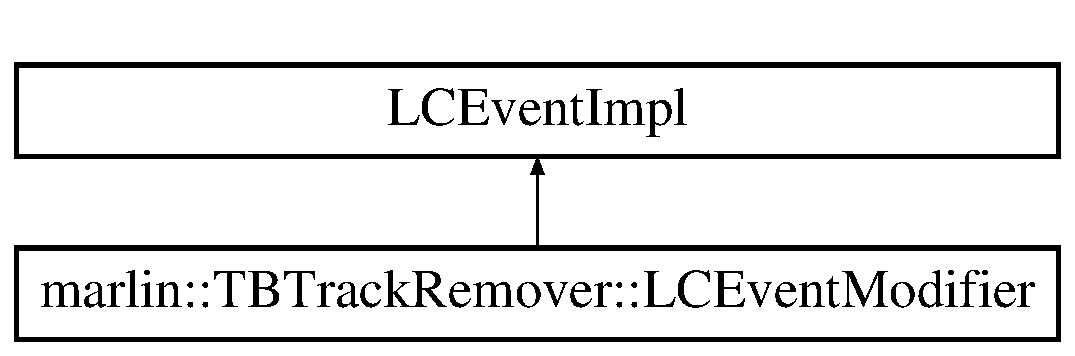
\includegraphics[height=2.000000cm]{classmarlin_1_1TBTrackRemover_1_1LCEventModifier}
\end{center}
\end{figure}
\subsection*{Static Public Member Functions}
\begin{DoxyCompactItemize}
\item 
static void {\bfseries delete\-Collection} (L\-C\-Event $\ast$r, const std\-::string \&name)\label{classmarlin_1_1TBTrackRemover_1_1LCEventModifier_adac30a804a963f47f0da9dff12be6a12}

\end{DoxyCompactItemize}


\subsection{Detailed Description}
Helper class to for the modification of the Event Header. 

Definition at line 72 of file T\-B\-Track\-Remover.\-hh.



The documentation for this class was generated from the following file\-:\begin{DoxyCompactItemize}
\item 
T\-B\-Track\-Remover.\-hh\end{DoxyCompactItemize}

\section{L\-C\-Payload$<$ Payload $>$ Class Template Reference}
\label{classLCPayload}\index{L\-C\-Payload$<$ Payload $>$@{L\-C\-Payload$<$ Payload $>$}}


Specific L\-C\-I\-O implementation of the interface to store generic user data.  




{\ttfamily \#include $<$L\-C\-Payload.\-hh$>$}

Inheritance diagram for L\-C\-Payload$<$ Payload $>$\-:\begin{figure}[H]
\begin{center}
\leavevmode
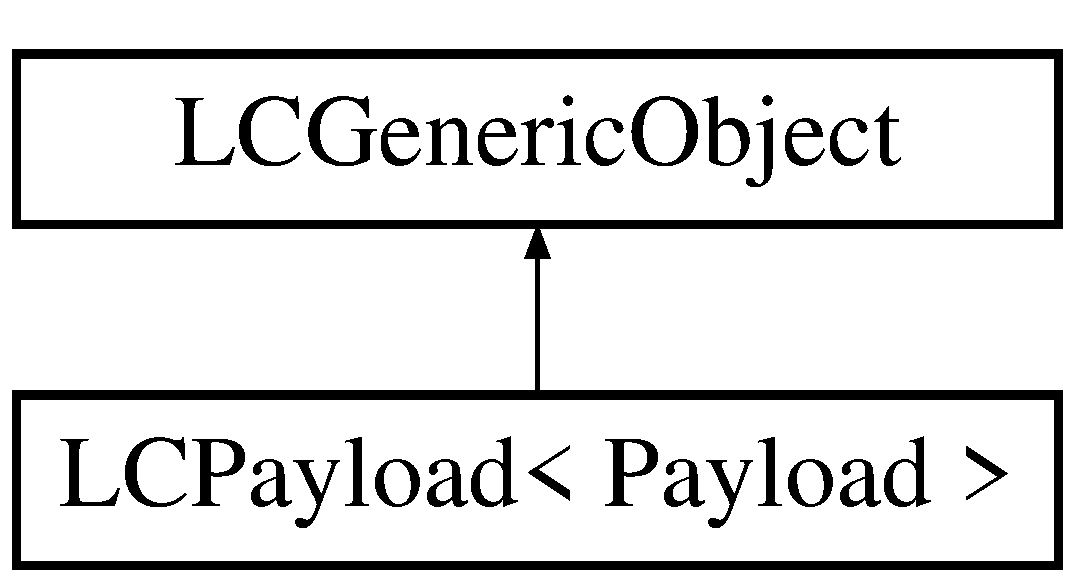
\includegraphics[height=2.000000cm]{classLCPayload}
\end{center}
\end{figure}
\subsection*{Public Member Functions}
\begin{DoxyCompactItemize}
\item 
{\bf L\-C\-Payload} ()\label{classLCPayload_a8b8d145b1753cabef13f6da15d957c39}

\begin{DoxyCompactList}\small\item\em Constructors. \end{DoxyCompactList}\item 
{\bfseries L\-C\-Payload} (const E\-V\-E\-N\-T\-::\-L\-C\-Generic\-Object $\ast$obj)\label{classLCPayload_abecb2b247eb9265510f784db83297806}

\item 
{\bfseries L\-C\-Payload} (const Payload \&c)\label{classLCPayload_a96860b56042d95ba0c4fa36aeef8c164}

\item 
{\bfseries L\-C\-Payload} (const Payload \&p, I\-M\-P\-L\-::\-L\-C\-Generic\-Object\-Impl \&obj)\label{classLCPayload_aa29b1863b733b5e544696fa29788f9c2}

\item 
virtual {\bf $\sim$\-L\-C\-Payload} ()\label{classLCPayload_ac1e66fabe1f9f65972ec738f7574e84c}

\begin{DoxyCompactList}\small\item\em Destructor. \end{DoxyCompactList}\item 
virtual void {\bf update} (const E\-V\-E\-N\-T\-::\-L\-C\-Generic\-Object $\ast$obj)\label{classLCPayload_a461543886a17454a20f92d685f8c8bdc}

\begin{DoxyCompactList}\small\item\em Update values within the object from an L\-C\-Generic\-Object. \end{DoxyCompactList}\item 
virtual E\-V\-E\-N\-T\-::\-L\-C\-Generic\-Object $\ast$ {\bf output} () const \label{classLCPayload_a438b42bdc529adc71a5c0bc960b32883}

\begin{DoxyCompactList}\small\item\em Create a new L\-C\-Generic\-Object and fill it. \end{DoxyCompactList}\item 
virtual void {\bf update} (const std\-::string \&file\-Name)\label{classLCPayload_a5fce76c90beebf958604253586bfd649}

\begin{DoxyCompactList}\small\item\em Update values within the object from a flat file. \end{DoxyCompactList}\item 
virtual void {\bf output} (const std\-::string \&file\-Name) const \label{classLCPayload_a891246b9b47aa64690632308f9af7a15}

\begin{DoxyCompactList}\small\item\em Create a new flat file and fill it. \end{DoxyCompactList}\item 
virtual int {\bf get\-N\-Int} () const \label{classLCPayload_a60bf414fbb56e82a7a8a405023f263b7}

\begin{DoxyCompactList}\small\item\em Number of integer values stored in this object. \end{DoxyCompactList}\item 
virtual int {\bf get\-N\-Float} () const \label{classLCPayload_adb8d459967c8cbd5e349cf0ceb233d1b}

\begin{DoxyCompactList}\small\item\em Number of float values stored in this object. \end{DoxyCompactList}\item 
virtual int {\bf get\-N\-Double} () const \label{classLCPayload_ab465cc9ebd35f82089fa980470eca413}

\begin{DoxyCompactList}\small\item\em Number of double values stored in this object. \end{DoxyCompactList}\item 
virtual int {\bf get\-Int\-Val} (int index) const \label{classLCPayload_a470d04e59dca5e575292f46170bc01d1}

\begin{DoxyCompactList}\small\item\em Returns the integer value for the given index. \end{DoxyCompactList}\item 
virtual float {\bf get\-Float\-Val} (int index) const \label{classLCPayload_a051df316ec7a181e623643adf9748c48}

\begin{DoxyCompactList}\small\item\em Returns the float value for the given index. \end{DoxyCompactList}\item 
virtual double {\bf get\-Double\-Val} (int index) const \label{classLCPayload_a6752bc94c3be02a767eae41599c2c663}

\begin{DoxyCompactList}\small\item\em Returns the double value for the given index. \end{DoxyCompactList}\item 
virtual void {\bf set\-Int\-Val} (unsigned index, int value)\label{classLCPayload_aa50e9b8b87d51d6482aa312348981448}

\begin{DoxyCompactList}\small\item\em Sets the integer value at the given index. \end{DoxyCompactList}\item 
virtual void {\bf set\-Float\-Val} (unsigned index, float value)\label{classLCPayload_a12e1b5355c7a8a06bb2a6057a709c75a}

\begin{DoxyCompactList}\small\item\em Sets the float value at the given index. \end{DoxyCompactList}\item 
virtual void {\bf set\-Double\-Val} (unsigned index, double value)\label{classLCPayload_a4d93cf109f053a0fd493c4989082f663}

\begin{DoxyCompactList}\small\item\em Sets the double value at the given index. \end{DoxyCompactList}\item 
virtual bool {\bf is\-Fixed\-Size} () const \label{classLCPayload_ac693f8e406129f62f897e30272ef1f9b}

\begin{DoxyCompactList}\small\item\em True if objects of the implementation class have a fixed size, i.\-e get\-N\-Int, get\-N\-Float and get\-N\-Double will return values that are constant during the lifetime of the object. \end{DoxyCompactList}\item 
virtual const std\-::string {\bf get\-Type\-Name} () const \label{classLCPayload_a7338d24c98c4aa99a5d720477e8301fa}

\begin{DoxyCompactList}\small\item\em The type name of the user class (typically the class name) \end{DoxyCompactList}\item 
virtual const std\-::string {\bf get\-Data\-Description} () const 
\begin{DoxyCompactList}\small\item\em The description string. \end{DoxyCompactList}\item 
virtual const Payload \& {\bf constants} () const \label{classLCPayload_a9893dcd67b1d2483e48fcb437aa0b29c}

\begin{DoxyCompactList}\small\item\em Access the actual data for read or write. \end{DoxyCompactList}\item 
virtual void {\bfseries constants} (const Payload \&p)\label{classLCPayload_a6396d80f22ca663e914843d438338b35}

\item 
virtual const Payload \& {\bfseries payload} () const \label{classLCPayload_a153acaff49e7286ae3514867bb8032c6}

\item 
virtual void {\bfseries payload} (const Payload \&p)\label{classLCPayload_ac51c5e8c33b60d49403b9326f61ff475}

\end{DoxyCompactItemize}
\subsection*{Protected Attributes}
\begin{DoxyCompactItemize}
\item 
Payload {\bfseries \-\_\-payload}\label{classLCPayload_a281072ee5a8fe9247b7ed45915236907}

\end{DoxyCompactItemize}


\subsection{Detailed Description}
\subsubsection*{template$<$class Payload$>$class L\-C\-Payload$<$ Payload $>$}

Specific L\-C\-I\-O implementation of the interface to store generic user data. 

\begin{DoxyAuthor}{Author}
dauncey 
\end{DoxyAuthor}
\begin{DoxyVersion}{Version}

\end{DoxyVersion}
\begin{DoxyParagraph}{Id\-:}
\doxyref{L\-C\-Payload.\-hh}{p.}{LCPayload_8hh_source},v 1.\-3 2009-\/03-\/24 11\-:40\-:43 dauncey Exp 
\end{DoxyParagraph}


Definition at line 19 of file L\-C\-Payload.\-hh.



\subsection{Member Function Documentation}
\index{L\-C\-Payload@{L\-C\-Payload}!get\-Data\-Description@{get\-Data\-Description}}
\index{get\-Data\-Description@{get\-Data\-Description}!LCPayload@{L\-C\-Payload}}
\subsubsection[{get\-Data\-Description}]{\setlength{\rightskip}{0pt plus 5cm}template$<$class Payload $>$ const std\-::string {\bf L\-C\-Payload}$<$ Payload $>$\-::get\-Data\-Description (
\begin{DoxyParamCaption}
{}
\end{DoxyParamCaption}
) const\hspace{0.3cm}{\ttfamily [virtual]}}\label{classLCPayload_a118d95b1a2c431153cc3691d29b18692}


The description string. 

A comma separated list of pairs of type identifier, one of 'i','f','d' followed by '\-:' and an attribute name, e.\-g. \char`\"{}i\-:cell\-Id,f\-:offset,f\-:gain\char`\"{}. 

Definition at line 342 of file L\-C\-Payload.\-hh.



The documentation for this class was generated from the following file\-:\begin{DoxyCompactItemize}
\item 
L\-C\-Payload.\-hh\end{DoxyCompactItemize}

\section{marlin\-:\-:Run\-Info\-Processor\-:\-:L\-C\-Run\-Modifier Class Reference}
\label{classmarlin_1_1RunInfoProcessor_1_1LCRunModifier}\index{marlin\-::\-Run\-Info\-Processor\-::\-L\-C\-Run\-Modifier@{marlin\-::\-Run\-Info\-Processor\-::\-L\-C\-Run\-Modifier}}


Helper class to for the modification of the Run Header.  


Inheritance diagram for marlin\-:\-:Run\-Info\-Processor\-:\-:L\-C\-Run\-Modifier\-:\begin{figure}[H]
\begin{center}
\leavevmode
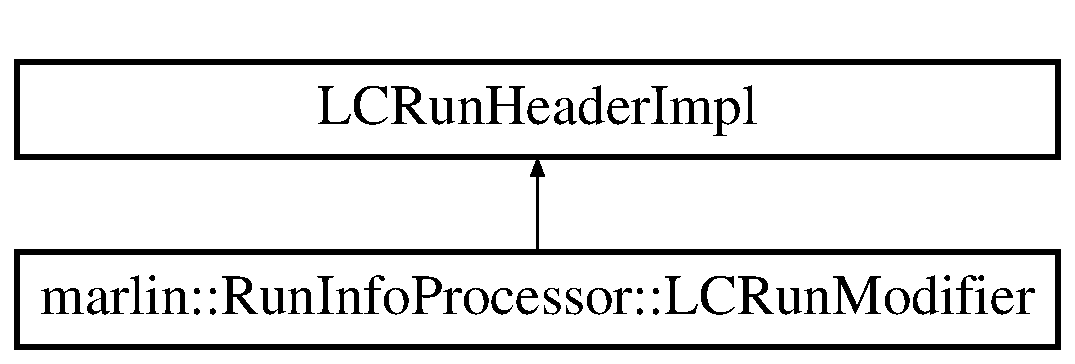
\includegraphics[height=2.000000cm]{classmarlin_1_1RunInfoProcessor_1_1LCRunModifier}
\end{center}
\end{figure}
\subsection*{Static Public Member Functions}
\begin{DoxyCompactItemize}
\item 
static void {\bfseries set\-Run} (L\-C\-Run\-Header $\ast$r, int n, std\-::string description)\label{classmarlin_1_1RunInfoProcessor_1_1LCRunModifier_ad5b4d3ac8439c98e21d6ec66de4ec8ab}

\end{DoxyCompactItemize}


\subsection{Detailed Description}
Helper class to for the modification of the Run Header. 

Definition at line 159 of file Run\-Info\-Processor.\-hh.



The documentation for this class was generated from the following file\-:\begin{DoxyCompactItemize}
\item 
Run\-Info\-Processor.\-hh\end{DoxyCompactItemize}

\section{L\-C\-Track\-Payload$<$ Payload $>$ Class Template Reference}
\label{classLCTrackPayload}\index{L\-C\-Track\-Payload$<$ Payload $>$@{L\-C\-Track\-Payload$<$ Payload $>$}}


Specific L\-C\-I\-O implementation of the interface to store generic user data.  




{\ttfamily \#include $<$L\-C\-Track\-Payload.\-hh$>$}

Inheritance diagram for L\-C\-Track\-Payload$<$ Payload $>$\-:\begin{figure}[H]
\begin{center}
\leavevmode
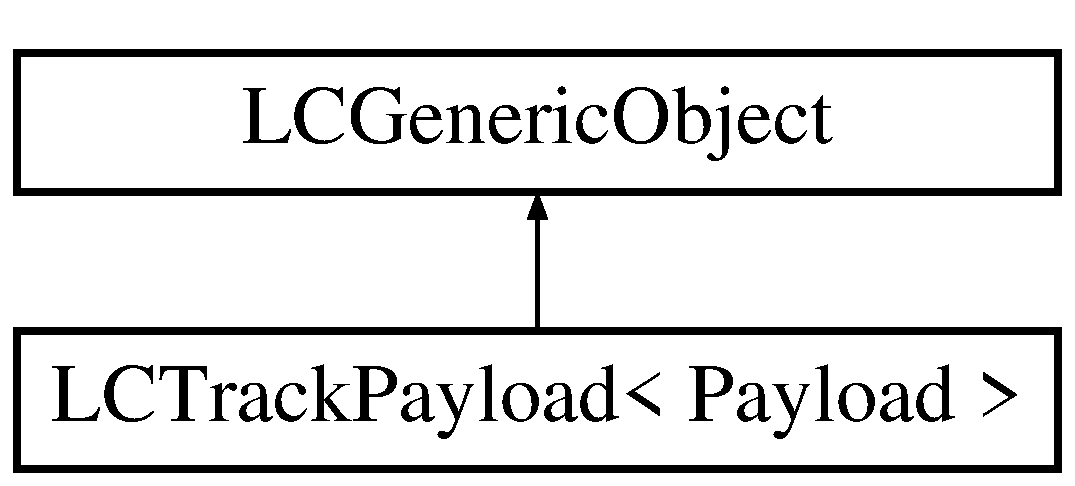
\includegraphics[height=2.000000cm]{classLCTrackPayload}
\end{center}
\end{figure}
\subsection*{Public Member Functions}
\begin{DoxyCompactItemize}
\item 
{\bf L\-C\-Track\-Payload} ()\label{classLCTrackPayload_a10aabc99033fe1163ec4bacd1f683e52}

\begin{DoxyCompactList}\small\item\em Constructors. \end{DoxyCompactList}\item 
{\bfseries L\-C\-Track\-Payload} (const E\-V\-E\-N\-T\-::\-L\-C\-Generic\-Object $\ast$obj)\label{classLCTrackPayload_a995d11dd83d9e9f10c2c178425ab96dc}

\item 
{\bfseries L\-C\-Track\-Payload} (const Payload \&c)\label{classLCTrackPayload_ac7283dc42793904ea2e6a61ad47e760f}

\item 
{\bfseries L\-C\-Track\-Payload} (const Payload \&p, I\-M\-P\-L\-::\-L\-C\-Generic\-Object\-Impl \&obj)\label{classLCTrackPayload_a64e99cf37fab6f26835ee47464379444}

\item 
virtual {\bf $\sim$\-L\-C\-Track\-Payload} ()\label{classLCTrackPayload_a76b84074f0064c45f8473662820d481d}

\begin{DoxyCompactList}\small\item\em Destructor. \end{DoxyCompactList}\item 
virtual void {\bf update} (const E\-V\-E\-N\-T\-::\-L\-C\-Generic\-Object $\ast$obj)\label{classLCTrackPayload_aea1a5317f1a5abd198c127638c2505da}

\begin{DoxyCompactList}\small\item\em Update values within the object from an L\-C\-Generic\-Object. \end{DoxyCompactList}\item 
virtual E\-V\-E\-N\-T\-::\-L\-C\-Generic\-Object $\ast$ {\bf output} () const \label{classLCTrackPayload_ad6359058eb2c59c82b10ca98fa90424a}

\begin{DoxyCompactList}\small\item\em Create a new L\-C\-Generic\-Object and fill it. \end{DoxyCompactList}\item 
virtual int {\bf get\-N\-Int} () const \label{classLCTrackPayload_ac6ce3cdeab53d7c8c098279a9598f3c1}

\begin{DoxyCompactList}\small\item\em Number of integer values stored in this object. \end{DoxyCompactList}\item 
virtual int {\bf get\-N\-Float} () const \label{classLCTrackPayload_a1eb3d42fd2ac6eac76dd2b0c76c54689}

\begin{DoxyCompactList}\small\item\em Number of float values stored in this object. \end{DoxyCompactList}\item 
virtual int {\bf get\-N\-Double} () const \label{classLCTrackPayload_a8c5dfa41f6430205758fa8eb30868771}

\begin{DoxyCompactList}\small\item\em Number of double values stored in this object. \end{DoxyCompactList}\item 
virtual int {\bf get\-Int\-Val} (int index) const \label{classLCTrackPayload_a4f6dc00e5a78eb37534c29545efad2d7}

\begin{DoxyCompactList}\small\item\em Returns the integer value for the given index. \end{DoxyCompactList}\item 
virtual float {\bf get\-Float\-Val} (int index) const \label{classLCTrackPayload_a47c0f1771fcfb56e86941c90449f88c8}

\begin{DoxyCompactList}\small\item\em Returns the float value for the given index. \end{DoxyCompactList}\item 
virtual double {\bf get\-Double\-Val} (int index) const \label{classLCTrackPayload_a7d2682a798e967dd00363dc90a1b1dcc}

\begin{DoxyCompactList}\small\item\em Returns the double value for the given index. \end{DoxyCompactList}\item 
virtual void {\bf set\-Int\-Val} (unsigned index, int value)\label{classLCTrackPayload_a4e92e7bfa326b29e1bc0bb8888d700e1}

\begin{DoxyCompactList}\small\item\em Sets the integer value at the given index. \end{DoxyCompactList}\item 
virtual void {\bf set\-Float\-Val} (unsigned index, float value)\label{classLCTrackPayload_ad92a24649bec4959158a57f709a35423}

\begin{DoxyCompactList}\small\item\em Sets the float value at the given index. \end{DoxyCompactList}\item 
virtual void {\bf set\-Double\-Val} (unsigned index, double value)\label{classLCTrackPayload_a23161fdc6b57a9fcd4d3a900bd333310}

\begin{DoxyCompactList}\small\item\em Sets the double value at the given index. \end{DoxyCompactList}\item 
virtual bool {\bf is\-Fixed\-Size} () const \label{classLCTrackPayload_aabc45cbe4ecf99f2031378c9cedfc804}

\begin{DoxyCompactList}\small\item\em True if objects of the implementation class have a fixed size, i.\-e get\-N\-Int, get\-N\-Float and get\-N\-Double will return values that are constant during the lifetime of the object. \end{DoxyCompactList}\item 
virtual const std\-::string {\bf get\-Type\-Name} () const \label{classLCTrackPayload_ab56a3408c7013b69adf621b0813fbbf9}

\begin{DoxyCompactList}\small\item\em The type name of the user class (typically the class name) \end{DoxyCompactList}\item 
virtual const std\-::string {\bf get\-Data\-Description} () const 
\begin{DoxyCompactList}\small\item\em The description string. \end{DoxyCompactList}\item 
virtual const Payload \& {\bf constants} () const \label{classLCTrackPayload_a1d0364cf45deb6c764ffecbe08e0cf84}

\begin{DoxyCompactList}\small\item\em Access the actual data for read or write. \end{DoxyCompactList}\item 
virtual void {\bfseries constants} (const Payload \&p)\label{classLCTrackPayload_a572f1162e50700b9f241e7ba0d80219f}

\item 
virtual const Payload \& {\bfseries payload} () const \label{classLCTrackPayload_a65557857fdc305d92c0e99b740effa9e}

\item 
virtual void {\bfseries payload} (const Payload \&p)\label{classLCTrackPayload_ab78efc5558a8c4a60776f37ce9a3982a}

\end{DoxyCompactItemize}
\subsection*{Protected Attributes}
\begin{DoxyCompactItemize}
\item 
Payload {\bfseries \-\_\-payload}\label{classLCTrackPayload_a89353b7b9de237aa375f1a7a94e59ad7}

\end{DoxyCompactItemize}


\subsection{Detailed Description}
\subsubsection*{template$<$class Payload$>$class L\-C\-Track\-Payload$<$ Payload $>$}

Specific L\-C\-I\-O implementation of the interface to store generic user data. 

\begin{DoxyAuthor}{Author}
dauncey 
\end{DoxyAuthor}
\begin{DoxyVersion}{Version}

\end{DoxyVersion}
\begin{DoxyParagraph}{Id\-:}
\doxyref{L\-C\-Track\-Payload.\-hh}{p.}{LCTrackPayload_8hh_source},v 1.\-1 2007-\/04-\/26 14\-:34\-:28 poeschl Exp 
\end{DoxyParagraph}


Definition at line 19 of file L\-C\-Track\-Payload.\-hh.



\subsection{Member Function Documentation}
\index{L\-C\-Track\-Payload@{L\-C\-Track\-Payload}!get\-Data\-Description@{get\-Data\-Description}}
\index{get\-Data\-Description@{get\-Data\-Description}!LCTrackPayload@{L\-C\-Track\-Payload}}
\subsubsection[{get\-Data\-Description}]{\setlength{\rightskip}{0pt plus 5cm}template$<$class Payload $>$ const std\-::string {\bf L\-C\-Track\-Payload}$<$ Payload $>$\-::get\-Data\-Description (
\begin{DoxyParamCaption}
{}
\end{DoxyParamCaption}
) const\hspace{0.3cm}{\ttfamily [virtual]}}\label{classLCTrackPayload_acad8e51a5ce7ccd79dc652c03177f091}


The description string. 

A comma separated list of pairs of type identifier, one of 'i','f','d' followed by '\-:' and an attribute name, e.\-g. \char`\"{}i\-:cell\-Id,f\-:offset,f\-:gain\char`\"{}. 

Definition at line 252 of file L\-C\-Track\-Payload.\-hh.



The documentation for this class was generated from the following file\-:\begin{DoxyCompactItemize}
\item 
L\-C\-Track\-Payload.\-hh\end{DoxyCompactItemize}

\section{T\-B\-Track\-:\-:Linear\-Fit\-Result Class Reference}
\label{classTBTrack_1_1LinearFitResult}\index{T\-B\-Track\-::\-Linear\-Fit\-Result@{T\-B\-Track\-::\-Linear\-Fit\-Result}}
\subsection*{Public Member Functions}
\begin{DoxyCompactItemize}
\item 
{\bfseries Linear\-Fit\-Result} (double c, int n, const T\-Vector\-D \&p, const T\-Matrix\-D\-Sym \&e)\label{classTBTrack_1_1LinearFitResult_a3e4ba61e44c68bcf81db05f704d5d5b1}

\item 
double {\bfseries chi\-Squared} () const \label{classTBTrack_1_1LinearFitResult_a036042e6787c607d0ee51b20044d52b9}

\item 
int {\bfseries number\-Of\-Dof} () const \label{classTBTrack_1_1LinearFitResult_ab41a070ef6c6e60a04f44e1ad833caa3}

\item 
double {\bfseries probability} () const \label{classTBTrack_1_1LinearFitResult_a750253e1904b159bee301eceb5f09f80}

\item 
const T\-Vector\-D \& {\bfseries parameters} () const \label{classTBTrack_1_1LinearFitResult_ae0ed921b62f6653de3531a406335c7c2}

\item 
const T\-Matrix\-D\-Sym \& {\bfseries errors} () const \label{classTBTrack_1_1LinearFitResult_aaef15bed0282bc3f5e8e2e59f0d611d6}

\item 
double {\bfseries probability} (const T\-Vector\-D \&p) const \label{classTBTrack_1_1LinearFitResult_a1fa9bf5b974dd4a0bc5d692c66bd820b}

\item 
std\-::ostream \& {\bfseries print} (std\-::ostream \&o=std\-::cout, const std\-::string \&s=\char`\"{}\char`\"{}) const \label{classTBTrack_1_1LinearFitResult_adafd249c515c0a59daa63513c7a5fb1c}

\end{DoxyCompactItemize}
\subsection*{Private Attributes}
\begin{DoxyCompactItemize}
\item 
double {\bfseries \-\_\-chi\-Squared}\label{classTBTrack_1_1LinearFitResult_a009140f1916c5f9fffbdde89e000fe94}

\item 
int {\bfseries \-\_\-number\-Of\-Dof}\label{classTBTrack_1_1LinearFitResult_a2a4b4553ede2fc2363e4beab085404c8}

\item 
T\-Vector\-D {\bfseries \-\_\-parameters}\label{classTBTrack_1_1LinearFitResult_aab3a876556b7afa7eb0492e30a51b56d}

\item 
T\-Matrix\-D\-Sym {\bfseries \-\_\-errors}\label{classTBTrack_1_1LinearFitResult_a71acc0645f990d05042ccd962cf36ef7}

\end{DoxyCompactItemize}


\subsection{Detailed Description}


Definition at line 15 of file Linear\-Fit\-Result.\-hh.



The documentation for this class was generated from the following files\-:\begin{DoxyCompactItemize}
\item 
Linear\-Fit\-Result.\-hh\item 
Linear\-Fit\-Result.\-cc\end{DoxyCompactItemize}

\section{T\-B\-Track\-:\-:Linear\-Fitter Class Reference}
\label{classTBTrack_1_1LinearFitter}\index{T\-B\-Track\-::\-Linear\-Fitter@{T\-B\-Track\-::\-Linear\-Fitter}}
\subsection*{Public Member Functions}
\begin{DoxyCompactItemize}
\item 
void {\bfseries fit\-Initialisation} (const T\-Matrix\-D \&z, const T\-Matrix\-D\-Sym \&e)\label{classTBTrack_1_1LinearFitter_af83e617778ace54723fba9d11eaad900}

\item 
const T\-Matrix\-D\-Sym \& {\bfseries error\-Matrix} () const \label{classTBTrack_1_1LinearFitter_ab3c00a9eb140ba63e0cae20e7db9df43}

\item 
const T\-Matrix\-D \& {\bfseries solution\-Matrix} () const \label{classTBTrack_1_1LinearFitter_adb053f46cd4b1cabd89aafb802b14b4e}

\item 
const T\-Matrix\-D\-Sym \& {\bfseries chi\-Squared\-Matrix} () const \label{classTBTrack_1_1LinearFitter_a941c09f4b9d2976aa9b14ac1c9d55ccd}

\item 
std\-::ostream \& {\bfseries print\-Initialisation} (std\-::ostream \&o=std\-::cout, const std\-::string \&s=\char`\"{}\char`\"{}) const \label{classTBTrack_1_1LinearFitter_a458de2b57f0b458e007fab1eb04a3b71}

\item 
{\bf Linear\-Fit\-Result} {\bfseries fit\-Result} (const T\-Vector\-D \&x) const \label{classTBTrack_1_1LinearFitter_a3609570379fc6b194cd8a576d5579be6}

\end{DoxyCompactItemize}
\subsection*{Private Attributes}
\begin{DoxyCompactItemize}
\item 
T\-Matrix\-D {\bfseries \-\_\-fit\-Values}\label{classTBTrack_1_1LinearFitter_a0d5ab614c1263e593037ebdd7fccf92d}

\item 
T\-Matrix\-D\-Sym {\bfseries \-\_\-error\-Matrix}\label{classTBTrack_1_1LinearFitter_a92f10ab1b7cc02975e9c84823e93af18}

\item 
T\-Matrix\-D {\bfseries \-\_\-solution\-Matrix}\label{classTBTrack_1_1LinearFitter_af166aa8136a2aa0f60f47fa2e984f2cd}

\item 
T\-Matrix\-D\-Sym {\bfseries \-\_\-chi\-Squared\-Matrix}\label{classTBTrack_1_1LinearFitter_a86f7868c45931d0cc11e150bb81761c4}

\end{DoxyCompactItemize}


\subsection{Detailed Description}


Definition at line 15 of file Linear\-Fitter.\-hh.



The documentation for this class was generated from the following files\-:\begin{DoxyCompactItemize}
\item 
Linear\-Fitter.\-hh\item 
Linear\-Fitter.\-cc\end{DoxyCompactItemize}

\section{T\-B\-Track\-:\-:Map\-Constants Class Reference}
\label{classTBTrack_1_1MapConstants}\index{T\-B\-Track\-::\-Map\-Constants@{T\-B\-Track\-::\-Map\-Constants}}
\subsection*{Public Types}
\begin{DoxyCompactItemize}
\item 
enum \{ {\bfseries number\-Of\-Ints} =1
 \}
\item 
enum \{ {\bfseries number\-Of\-Floats} =0
 \}
\item 
enum \{ {\bfseries number\-Of\-Doubles} =0
 \}
\end{DoxyCompactItemize}
\subsection*{Public Member Functions}
\begin{DoxyCompactItemize}
\item 
{\bfseries Map\-Constants} (int p=0)\label{classTBTrack_1_1MapConstants_ad6a908a71ad6e73996a27429b7ba4485}

\item 
std\-::ostream \& {\bfseries print} (std\-::ostream \&o=std\-::cout, const std\-::string \&s=\char`\"{}\char`\"{}) const \label{classTBTrack_1_1MapConstants_abf0ecdc32902053ca7bacf7ab68d6166}

\item 
const int $\ast$ {\bfseries int\-Data} () const \label{classTBTrack_1_1MapConstants_aeaffabb97fe13e54bca6a2ccfcf5dcf4}

\item 
int $\ast$ {\bfseries int\-Data} ()\label{classTBTrack_1_1MapConstants_a64090ab098d7b42996eb37ac0181c6d9}

\item 
const float $\ast$ {\bfseries float\-Data} () const \label{classTBTrack_1_1MapConstants_a5db3dc38042fe8bc9fd1346eddbf2b43}

\item 
float $\ast$ {\bfseries float\-Data} ()\label{classTBTrack_1_1MapConstants_a25791641151a9a929d1cc7d9cb080976}

\item 
const double $\ast$ {\bfseries double\-Data} () const \label{classTBTrack_1_1MapConstants_a2dc86123f3989ad6f8e633aacec4c918}

\item 
double $\ast$ {\bfseries double\-Data} ()\label{classTBTrack_1_1MapConstants_a0b3f2db804b686ebd71e35d718564853}

\end{DoxyCompactItemize}
\subsection*{Private Attributes}
\begin{DoxyCompactItemize}
\item 
int {\bfseries \-\_\-period}\label{classTBTrack_1_1MapConstants_a136a931938bf1830db32ecd17745e4a5}

\end{DoxyCompactItemize}


\subsection{Detailed Description}


Definition at line 12 of file Map\-Constants.\-hh.



The documentation for this class was generated from the following files\-:\begin{DoxyCompactItemize}
\item 
Map\-Constants.\-hh\item 
Map\-Constants.\-cc\end{DoxyCompactItemize}

\section{marlin\-:\-:M\-C\-Run\-Time\-Processor Class Reference}
\label{classmarlin_1_1MCRunTimeProcessor}\index{marlin\-::\-M\-C\-Run\-Time\-Processor@{marlin\-::\-M\-C\-Run\-Time\-Processor}}
Inheritance diagram for marlin\-:\-:M\-C\-Run\-Time\-Processor\-:\begin{figure}[H]
\begin{center}
\leavevmode
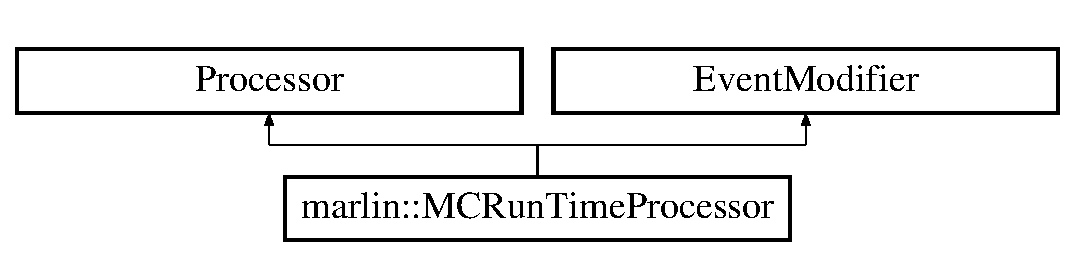
\includegraphics[height=2.000000cm]{classmarlin_1_1MCRunTimeProcessor}
\end{center}
\end{figure}
\subsection*{Public Member Functions}
\begin{DoxyCompactItemize}
\item 
virtual Processor $\ast$ {\bfseries new\-Processor} ()\label{classmarlin_1_1MCRunTimeProcessor_afaa7a8f8af2e6d40734992523adb0f18}

\item 
virtual const std\-::string \& {\bfseries name} () const \label{classmarlin_1_1MCRunTimeProcessor_a594976d07353672f85e23f50bc2c0183}

\item 
virtual void {\bfseries modify\-Event} (L\-C\-Event $\ast$evt)\label{classmarlin_1_1MCRunTimeProcessor_a51c9d9bf4f8b66e2c3b82f31f0f26bba}

\item 
virtual void {\bfseries init} ()\label{classmarlin_1_1MCRunTimeProcessor_a645e036d00d0ac4f016a6fb8d33f40c1}

\item 
virtual void {\bfseries process\-Run\-Header} (L\-C\-Run\-Header $\ast$run)\label{classmarlin_1_1MCRunTimeProcessor_a94ffb5e4ec27a97de5a30bc5c43f0655}

\item 
virtual void {\bfseries check} (L\-C\-Event $\ast$evt)\label{classmarlin_1_1MCRunTimeProcessor_afcac2282e9028e447afc453cb0f3cc5d}

\item 
virtual void {\bfseries end} ()\label{classmarlin_1_1MCRunTimeProcessor_a1b72a2ae28eb11cf4460b765a0ef0e01}

\end{DoxyCompactItemize}
\subsection*{Private Attributes}
\begin{DoxyCompactItemize}
\item 
std\-::string {\bfseries \-\_\-db\-Init}\label{classmarlin_1_1MCRunTimeProcessor_a4e743478c041ee93d3256134520e3c49}

\item 
std\-::string {\bfseries \-\_\-folder\-Run\-Time}\label{classmarlin_1_1MCRunTimeProcessor_a30df635002d96b32291813aa3f91d585}

\item 
std\-::string {\bfseries \-\_\-folder\-Location}\label{classmarlin_1_1MCRunTimeProcessor_a2be1163f77699025a223cd1ebb1040f4}

\item 
Run\-Location\-Whizard $\ast$ {\bfseries \-\_\-runlocationwhizard}\label{classmarlin_1_1MCRunTimeProcessor_a29bd192e54ae09e3b3dd9240b2f7ac23}

\item 
Run\-Time\-Whizard $\ast$ {\bfseries \-\_\-runtimewhizard}\label{classmarlin_1_1MCRunTimeProcessor_a136eebf08c52e00b691e7ad562ebae76}

\item 
int {\bfseries \-\_\-run\-Number}\label{classmarlin_1_1MCRunTimeProcessor_a9e3dea800b1c0e2104a00a5007714ddd}

\item 
int {\bfseries \-\_\-savety\-Margin}\label{classmarlin_1_1MCRunTimeProcessor_ae97bf35ad864f1bafba1864de9d03bc5}

\item 
U\-T\-I\-L\-::\-L\-C\-Time {\bfseries \-\_\-event\-Time}\label{classmarlin_1_1MCRunTimeProcessor_a119971e6c2b38d2ff99240191f82ce09}

\end{DoxyCompactItemize}


\subsection{Detailed Description}


Definition at line 18 of file M\-C\-Run\-Time\-Processor.\-hh.



The documentation for this class was generated from the following files\-:\begin{DoxyCompactItemize}
\item 
M\-C\-Run\-Time\-Processor.\-hh\item 
M\-C\-Run\-Time\-Processor.\-cc\end{DoxyCompactItemize}

\section{C\-A\-L\-I\-C\-E\-:\-:Mip\-Select Class Reference}
\label{classCALICE_1_1MipSelect}\index{C\-A\-L\-I\-C\-E\-::\-Mip\-Select@{C\-A\-L\-I\-C\-E\-::\-Mip\-Select}}


Simple class to try to select hits resulting from one mip.  




{\ttfamily \#include $<$Mip\-Select.\-hh$>$}

Inheritance diagram for C\-A\-L\-I\-C\-E\-:\-:Mip\-Select\-:\begin{figure}[H]
\begin{center}
\leavevmode
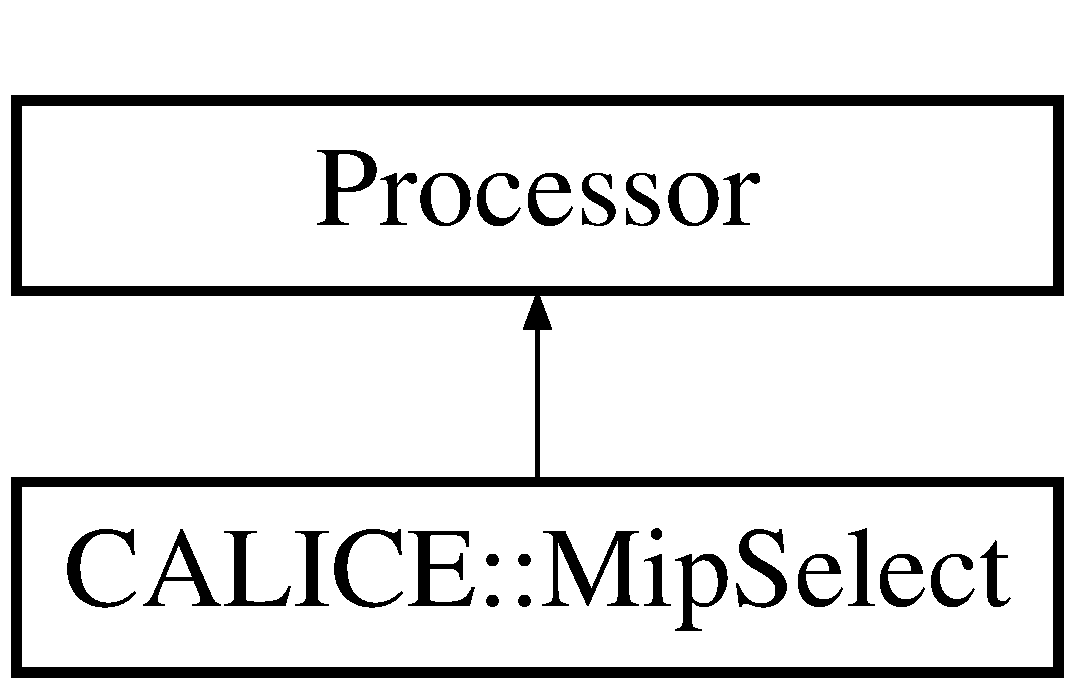
\includegraphics[height=2.000000cm]{classCALICE_1_1MipSelect}
\end{center}
\end{figure}
\subsection*{Public Member Functions}
\begin{DoxyCompactItemize}
\item 
Processor $\ast$ {\bfseries new\-Processor} ()\label{classCALICE_1_1MipSelect_a0f4980cc56e6302a351f1029f1259655}

\item 
{\bf Mip\-Select} ()
\begin{DoxyCompactList}\small\item\em Select Mips . \end{DoxyCompactList}\item 
void {\bf init} ()
\begin{DoxyCompactList}\small\item\em Called at the begin of the job before anything is read. \end{DoxyCompactList}\item 
void {\bf process\-Run\-Header} (L\-C\-Run\-Header $\ast$run)
\begin{DoxyCompactList}\small\item\em Called for every run, e.\-g. \end{DoxyCompactList}\item 
void {\bf process\-Event} (L\-C\-Event $\ast$evt\-P)\label{classCALICE_1_1MipSelect_a4fda653147df06d659939dfe36aceb34}

\begin{DoxyCompactList}\small\item\em Called for every event -\/ the working horse. \end{DoxyCompactList}\item 
void {\bfseries end} ()\label{classCALICE_1_1MipSelect_aa1e14b5e9e444acae637f2cbcc0511e0}

\end{DoxyCompactItemize}
\subsection*{Protected Attributes}
\begin{DoxyCompactItemize}
\item 
Int\-Vec {\bf \-\_\-n\-Hits}
\begin{DoxyCompactList}\small\item\em minimum and maximum required number of hits for a cluster (Marlin processor parameter). \end{DoxyCompactList}\item 
Float\-\_\-t {\bf \-\_\-max\-Dist}
\begin{DoxyCompactList}\small\item\em the maximum distance between hits considered to be close (Marlin processor parameter). \end{DoxyCompactList}\item 
Float\-Vec {\bf \-\_\-cluster\-Energy}
\begin{DoxyCompactList}\small\item\em minimum and maximum required cluster energy (Marlin processor parameter). \end{DoxyCompactList}\item 
Float\-\_\-t {\bf \-\_\-max\-Chi2}
\begin{DoxyCompactList}\small\item\em minimum required chi2 of the x and y straight line fits (Marlin processor parameter). \end{DoxyCompactList}\item 
Float\-\_\-t {\bf \-\_\-w0}
\begin{DoxyCompactList}\small\item\em Cut parameter which defines the energy threshold of hits considered in the centre-\/of-\/gravity determination (Marlin processor parameter). \end{DoxyCompactList}\item 
Float\-Vec {\bf \-\_\-pos\-Error}
\begin{DoxyCompactList}\small\item\em Error assigned to the cluster barycentre (marlin processor parameter). \end{DoxyCompactList}\item 
std\-::string {\bf \-\_\-col\-Name}\label{classCALICE_1_1MipSelect_ac9ae37843e4f13fdb0339917b36e3bb9}

\begin{DoxyCompactList}\small\item\em name of the hit input collection (Marlin processor parameter) \end{DoxyCompactList}\item 
std\-::string {\bf \-\_\-cluster\-Col\-Name}\label{classCALICE_1_1MipSelect_ad9094c81faee001d8cb848cbd0da5ac4}

\begin{DoxyCompactList}\small\item\em name of the cluster output collection (Marlin processor parameter) \end{DoxyCompactList}\end{DoxyCompactItemize}
\subsection*{Private Attributes}
\begin{DoxyCompactItemize}
\item 
std\-::vector$<$ U\-Int\-\_\-t $>$ {\bf \-\_\-isolated\-Hits}\label{classCALICE_1_1MipSelect_a9e44a652e454927b32108da491368eec}

\begin{DoxyCompactList}\small\item\em temporary buffer \end{DoxyCompactList}\end{DoxyCompactItemize}


\subsection{Detailed Description}
Simple class to try to select hits resulting from one mip. 

This processor tries to find hits in the chosen hit collection which are close together. If the number adjacent hits is large enough a cluster is created. \begin{DoxyRefDesc}{Todo}
\item[{\bf Todo}]\-: add shower shape criterium, maximum number of tolerated hits \end{DoxyRefDesc}


Definition at line 28 of file Mip\-Select.\-hh.



\subsection{Constructor \& Destructor Documentation}
\index{C\-A\-L\-I\-C\-E\-::\-Mip\-Select@{C\-A\-L\-I\-C\-E\-::\-Mip\-Select}!Mip\-Select@{Mip\-Select}}
\index{Mip\-Select@{Mip\-Select}!CALICE::MipSelect@{C\-A\-L\-I\-C\-E\-::\-Mip\-Select}}
\subsubsection[{Mip\-Select}]{\setlength{\rightskip}{0pt plus 5cm}C\-A\-L\-I\-C\-E\-::\-Mip\-Select\-::\-Mip\-Select (
\begin{DoxyParamCaption}
{}
\end{DoxyParamCaption}
)}\label{classCALICE_1_1MipSelect_a187a4421470be1e416ad1aaffabdab45}


Select Mips . 

Mip tracks are search within the calorimeter hits. Developped for cosmics. 

Definition at line 42 of file Mip\-Select.\-cc.



References \-\_\-cluster\-Col\-Name, \-\_\-cluster\-Energy, \-\_\-col\-Name, \-\_\-max\-Chi2, \-\_\-max\-Dist, \-\_\-n\-Hits, \-\_\-pos\-Error, and \-\_\-w0.



\subsection{Member Function Documentation}
\index{C\-A\-L\-I\-C\-E\-::\-Mip\-Select@{C\-A\-L\-I\-C\-E\-::\-Mip\-Select}!init@{init}}
\index{init@{init}!CALICE::MipSelect@{C\-A\-L\-I\-C\-E\-::\-Mip\-Select}}
\subsubsection[{init}]{\setlength{\rightskip}{0pt plus 5cm}void C\-A\-L\-I\-C\-E\-::\-Mip\-Select\-::init (
\begin{DoxyParamCaption}
{}
\end{DoxyParamCaption}
)}\label{classCALICE_1_1MipSelect_a6e9d97e8a6a621de6803dac121a9662b}


Called at the begin of the job before anything is read. 

Use to initialize the processor, e.\-g. book histograms. 

Definition at line 176 of file Mip\-Select.\-cc.



References \-\_\-cluster\-Energy, and \-\_\-n\-Hits.

\index{C\-A\-L\-I\-C\-E\-::\-Mip\-Select@{C\-A\-L\-I\-C\-E\-::\-Mip\-Select}!process\-Run\-Header@{process\-Run\-Header}}
\index{process\-Run\-Header@{process\-Run\-Header}!CALICE::MipSelect@{C\-A\-L\-I\-C\-E\-::\-Mip\-Select}}
\subsubsection[{process\-Run\-Header}]{\setlength{\rightskip}{0pt plus 5cm}void C\-A\-L\-I\-C\-E\-::\-Mip\-Select\-::process\-Run\-Header (
\begin{DoxyParamCaption}
\item[{L\-C\-Run\-Header $\ast$}]{run}
\end{DoxyParamCaption}
)\hspace{0.3cm}{\ttfamily [inline]}}\label{classCALICE_1_1MipSelect_af4ddc35f44aa0c65145e592fba7abb64}


Called for every run, e.\-g. 

overwrite to initialize run dependent histograms. 

Definition at line 46 of file Mip\-Select.\-hh.



\subsection{Field Documentation}
\index{C\-A\-L\-I\-C\-E\-::\-Mip\-Select@{C\-A\-L\-I\-C\-E\-::\-Mip\-Select}!\-\_\-cluster\-Energy@{\-\_\-cluster\-Energy}}
\index{\-\_\-cluster\-Energy@{\-\_\-cluster\-Energy}!CALICE::MipSelect@{C\-A\-L\-I\-C\-E\-::\-Mip\-Select}}
\subsubsection[{\-\_\-cluster\-Energy}]{\setlength{\rightskip}{0pt plus 5cm}Float\-Vec C\-A\-L\-I\-C\-E\-::\-Mip\-Select\-::\-\_\-cluster\-Energy\hspace{0.3cm}{\ttfamily [protected]}}\label{classCALICE_1_1MipSelect_a4724ccf37d271a114791a2d0d5575cb9}


minimum and maximum required cluster energy (Marlin processor parameter). 



Definition at line 57 of file Mip\-Select.\-hh.



Referenced by init(), Mip\-Select(), and process\-Event().

\index{C\-A\-L\-I\-C\-E\-::\-Mip\-Select@{C\-A\-L\-I\-C\-E\-::\-Mip\-Select}!\-\_\-max\-Chi2@{\-\_\-max\-Chi2}}
\index{\-\_\-max\-Chi2@{\-\_\-max\-Chi2}!CALICE::MipSelect@{C\-A\-L\-I\-C\-E\-::\-Mip\-Select}}
\subsubsection[{\-\_\-max\-Chi2}]{\setlength{\rightskip}{0pt plus 5cm}Float\-\_\-t C\-A\-L\-I\-C\-E\-::\-Mip\-Select\-::\-\_\-max\-Chi2\hspace{0.3cm}{\ttfamily [protected]}}\label{classCALICE_1_1MipSelect_a9ad0ff3988f10698ba6398158fdba7d3}


minimum required chi2 of the x and y straight line fits (Marlin processor parameter). 



Definition at line 58 of file Mip\-Select.\-hh.



Referenced by Mip\-Select(), and process\-Event().

\index{C\-A\-L\-I\-C\-E\-::\-Mip\-Select@{C\-A\-L\-I\-C\-E\-::\-Mip\-Select}!\-\_\-max\-Dist@{\-\_\-max\-Dist}}
\index{\-\_\-max\-Dist@{\-\_\-max\-Dist}!CALICE::MipSelect@{C\-A\-L\-I\-C\-E\-::\-Mip\-Select}}
\subsubsection[{\-\_\-max\-Dist}]{\setlength{\rightskip}{0pt plus 5cm}Float\-\_\-t C\-A\-L\-I\-C\-E\-::\-Mip\-Select\-::\-\_\-max\-Dist\hspace{0.3cm}{\ttfamily [protected]}}\label{classCALICE_1_1MipSelect_af5b5c0952ac42edf3e33ccc3354ce999}


the maximum distance between hits considered to be close (Marlin processor parameter). 



Definition at line 56 of file Mip\-Select.\-hh.



Referenced by Mip\-Select(), and process\-Event().

\index{C\-A\-L\-I\-C\-E\-::\-Mip\-Select@{C\-A\-L\-I\-C\-E\-::\-Mip\-Select}!\-\_\-n\-Hits@{\-\_\-n\-Hits}}
\index{\-\_\-n\-Hits@{\-\_\-n\-Hits}!CALICE::MipSelect@{C\-A\-L\-I\-C\-E\-::\-Mip\-Select}}
\subsubsection[{\-\_\-n\-Hits}]{\setlength{\rightskip}{0pt plus 5cm}Int\-Vec C\-A\-L\-I\-C\-E\-::\-Mip\-Select\-::\-\_\-n\-Hits\hspace{0.3cm}{\ttfamily [protected]}}\label{classCALICE_1_1MipSelect_a9942825c9ee70c394f78dde00c43c8ef}


minimum and maximum required number of hits for a cluster (Marlin processor parameter). 



Definition at line 55 of file Mip\-Select.\-hh.



Referenced by init(), Mip\-Select(), and process\-Event().

\index{C\-A\-L\-I\-C\-E\-::\-Mip\-Select@{C\-A\-L\-I\-C\-E\-::\-Mip\-Select}!\-\_\-pos\-Error@{\-\_\-pos\-Error}}
\index{\-\_\-pos\-Error@{\-\_\-pos\-Error}!CALICE::MipSelect@{C\-A\-L\-I\-C\-E\-::\-Mip\-Select}}
\subsubsection[{\-\_\-pos\-Error}]{\setlength{\rightskip}{0pt plus 5cm}Float\-Vec C\-A\-L\-I\-C\-E\-::\-Mip\-Select\-::\-\_\-pos\-Error\hspace{0.3cm}{\ttfamily [protected]}}\label{classCALICE_1_1MipSelect_a47f1821c1518e00d403d026c5b1eb848}


Error assigned to the cluster barycentre (marlin processor parameter). 



Definition at line 62 of file Mip\-Select.\-hh.



Referenced by Mip\-Select(), and process\-Event().

\index{C\-A\-L\-I\-C\-E\-::\-Mip\-Select@{C\-A\-L\-I\-C\-E\-::\-Mip\-Select}!\-\_\-w0@{\-\_\-w0}}
\index{\-\_\-w0@{\-\_\-w0}!CALICE::MipSelect@{C\-A\-L\-I\-C\-E\-::\-Mip\-Select}}
\subsubsection[{\-\_\-w0}]{\setlength{\rightskip}{0pt plus 5cm}Float\-\_\-t C\-A\-L\-I\-C\-E\-::\-Mip\-Select\-::\-\_\-w0\hspace{0.3cm}{\ttfamily [protected]}}\label{classCALICE_1_1MipSelect_ae601de1184f473e69224607d827436a3}


Cut parameter which defines the energy threshold of hits considered in the centre-\/of-\/gravity determination (Marlin processor parameter). 



Definition at line 59 of file Mip\-Select.\-hh.



Referenced by Mip\-Select(), and process\-Event().



The documentation for this class was generated from the following files\-:\begin{DoxyCompactItemize}
\item 
Mip\-Select.\-hh\item 
Mip\-Select.\-cc\end{DoxyCompactItemize}

\section{C\-A\-L\-I\-C\-E\-:\-:Module\-Index\-Reverse\-Lookup Class Reference}
\label{classCALICE_1_1ModuleIndexReverseLookup}\index{C\-A\-L\-I\-C\-E\-::\-Module\-Index\-Reverse\-Lookup@{C\-A\-L\-I\-C\-E\-::\-Module\-Index\-Reverse\-Lookup}}


Creates huge arrays which allows to find out the module and the cell index using the Mokka conform geometrical index.  




{\ttfamily \#include $<$Module\-Index\-Reverse\-Lookup.\-hh$>$}

\subsection*{Public Member Functions}
\begin{DoxyCompactItemize}
\item 
void {\bf create\-Index\-Reverse\-Lookup} (const Mapping\-And\-Alignment \&mapping)
\begin{DoxyCompactList}\small\item\em Create a huge arrays which contains for each cell the module and the cell index. \end{DoxyCompactList}\item 
pair$<$ U\-Int\-\_\-t, U\-Int\-\_\-t $>$ {\bf get\-Module\-And\-Cell\-Index} (const Mapping\-And\-Alignment \&mapping, const Cell\-Index \&a\-\_\-cell\-\_\-index) const 
\begin{DoxyCompactList}\small\item\em Return the module and cell index for the given Mokka conform geometrical cell index. \end{DoxyCompactList}\end{DoxyCompactItemize}
\subsection*{Protected Types}
\begin{DoxyCompactItemize}
\item 
typedef {\bf Simple\-Array\-\_\-t}\\*
$<$ {\bf Simple\-Array\-\_\-t}$<$ {\bf Simple\-Array\-\_\-t}\\*
$<$ {\bf Simple\-Array\-\_\-t}$<$ unsigned \\*
short $>$ $>$ $>$ $>$ {\bfseries Cell\-Index\-Array\-\_\-t}\label{classCALICE_1_1ModuleIndexReverseLookup_a3cb8a61f3dc239ac5ffbee685bf6988f}

\end{DoxyCompactItemize}
\subsection*{Protected Attributes}
\begin{DoxyCompactItemize}
\item 
{\bf Simple\-Array\-\_\-t}$<$ {\bf Simple\-Array\-\_\-t}\\*
$<$ {\bf Simple\-Array\-\_\-t}$<$ unsigned \\*
short $>$ $>$ $>$ {\bf \-\_\-module\-Index\-Array}
\begin{DoxyCompactList}\small\item\em Array which contains for each layer and wafer row and column the module index. \end{DoxyCompactList}\item 
{\bf Simple\-Array\-\_\-t}$<$ {\bf Cell\-Index\-Array\-\_\-t} $>$ {\bf \-\_\-module\-Type\-Array}
\begin{DoxyCompactList}\small\item\em Array which contains for each module type the cell indices for a pad of a given wafer, pad row and column. \end{DoxyCompactList}\end{DoxyCompactItemize}


\subsection{Detailed Description}
Creates huge arrays which allows to find out the module and the cell index using the Mokka conform geometrical index. 

Definition at line 9 of file Module\-Index\-Reverse\-Lookup.\-hh.



\subsection{Member Function Documentation}
\index{C\-A\-L\-I\-C\-E\-::\-Module\-Index\-Reverse\-Lookup@{C\-A\-L\-I\-C\-E\-::\-Module\-Index\-Reverse\-Lookup}!create\-Index\-Reverse\-Lookup@{create\-Index\-Reverse\-Lookup}}
\index{create\-Index\-Reverse\-Lookup@{create\-Index\-Reverse\-Lookup}!CALICE::ModuleIndexReverseLookup@{C\-A\-L\-I\-C\-E\-::\-Module\-Index\-Reverse\-Lookup}}
\subsubsection[{create\-Index\-Reverse\-Lookup}]{\setlength{\rightskip}{0pt plus 5cm}void C\-A\-L\-I\-C\-E\-::\-Module\-Index\-Reverse\-Lookup\-::create\-Index\-Reverse\-Lookup (
\begin{DoxyParamCaption}
\item[{const Mapping\-And\-Alignment \&}]{mapping}
\end{DoxyParamCaption}
)}\label{classCALICE_1_1ModuleIndexReverseLookup_a2bd62812d099ee99ec7cd26c8e25b39c}


Create a huge arrays which contains for each cell the module and the cell index. 

The array which contains the cell indices uses the module type, the wafer and pad row and column indices. The array which contains the module indices uses the wafer row and column index. 

Definition at line 10 of file Module\-Index\-Reverse\-Lookup.\-cc.



References \-\_\-module\-Index\-Array, and \-\_\-module\-Type\-Array.

\index{C\-A\-L\-I\-C\-E\-::\-Module\-Index\-Reverse\-Lookup@{C\-A\-L\-I\-C\-E\-::\-Module\-Index\-Reverse\-Lookup}!get\-Module\-And\-Cell\-Index@{get\-Module\-And\-Cell\-Index}}
\index{get\-Module\-And\-Cell\-Index@{get\-Module\-And\-Cell\-Index}!CALICE::ModuleIndexReverseLookup@{C\-A\-L\-I\-C\-E\-::\-Module\-Index\-Reverse\-Lookup}}
\subsubsection[{get\-Module\-And\-Cell\-Index}]{\setlength{\rightskip}{0pt plus 5cm}pair$<$U\-Int\-\_\-t, U\-Int\-\_\-t$>$ C\-A\-L\-I\-C\-E\-::\-Module\-Index\-Reverse\-Lookup\-::get\-Module\-And\-Cell\-Index (
\begin{DoxyParamCaption}
\item[{const Mapping\-And\-Alignment \&}]{mapping, }
\item[{const Cell\-Index \&}]{a\-\_\-cell\-\_\-index}
\end{DoxyParamCaption}
) const\hspace{0.3cm}{\ttfamily [inline]}}\label{classCALICE_1_1ModuleIndexReverseLookup_a639f10b89a671e6259c9e2d3ae98965f}


Return the module and cell index for the given Mokka conform geometrical cell index. 


\begin{DoxyParams}{Parameters}
{\em mapping} & reference to the mapping object. \\
\hline
{\em a\-\_\-cell\-\_\-index} & the Mokka conform geometrical cell index \\
\hline
\end{DoxyParams}
\begin{DoxyReturn}{Returns}
the module index and the cell index on the module. The module index is the index in the list of defined module locations (coditions datae). The cell index is the index of the cells on the module. The pads are multiplexed on 12(6) lines (readout chips). First the 12(6) cells of the fist sample are stored than the cells of next sample. 
\end{DoxyReturn}
\#ifdef B\-O\-U\-N\-D\-A\-R\-Y\-\_\-\-C\-H\-E\-C\-K 

Definition at line 31 of file Module\-Index\-Reverse\-Lookup.\-hh.



References \-\_\-module\-Index\-Array, and \-\_\-module\-Type\-Array.



\subsection{Field Documentation}
\index{C\-A\-L\-I\-C\-E\-::\-Module\-Index\-Reverse\-Lookup@{C\-A\-L\-I\-C\-E\-::\-Module\-Index\-Reverse\-Lookup}!\-\_\-module\-Index\-Array@{\-\_\-module\-Index\-Array}}
\index{\-\_\-module\-Index\-Array@{\-\_\-module\-Index\-Array}!CALICE::ModuleIndexReverseLookup@{C\-A\-L\-I\-C\-E\-::\-Module\-Index\-Reverse\-Lookup}}
\subsubsection[{\-\_\-module\-Index\-Array}]{\setlength{\rightskip}{0pt plus 5cm}{\bf Simple\-Array\-\_\-t}$<$ {\bf Simple\-Array\-\_\-t}$<$ {\bf Simple\-Array\-\_\-t}$<$ unsigned short $>$ $>$ $>$ C\-A\-L\-I\-C\-E\-::\-Module\-Index\-Reverse\-Lookup\-::\-\_\-module\-Index\-Array\hspace{0.3cm}{\ttfamily [protected]}}\label{classCALICE_1_1ModuleIndexReverseLookup_a6f4c66de3a572faa169b6d8f605e7e2f}


Array which contains for each layer and wafer row and column the module index. 



Definition at line 81 of file Module\-Index\-Reverse\-Lookup.\-hh.



Referenced by create\-Index\-Reverse\-Lookup(), and get\-Module\-And\-Cell\-Index().

\index{C\-A\-L\-I\-C\-E\-::\-Module\-Index\-Reverse\-Lookup@{C\-A\-L\-I\-C\-E\-::\-Module\-Index\-Reverse\-Lookup}!\-\_\-module\-Type\-Array@{\-\_\-module\-Type\-Array}}
\index{\-\_\-module\-Type\-Array@{\-\_\-module\-Type\-Array}!CALICE::ModuleIndexReverseLookup@{C\-A\-L\-I\-C\-E\-::\-Module\-Index\-Reverse\-Lookup}}
\subsubsection[{\-\_\-module\-Type\-Array}]{\setlength{\rightskip}{0pt plus 5cm}{\bf Simple\-Array\-\_\-t}$<$ {\bf Cell\-Index\-Array\-\_\-t} $>$ C\-A\-L\-I\-C\-E\-::\-Module\-Index\-Reverse\-Lookup\-::\-\_\-module\-Type\-Array\hspace{0.3cm}{\ttfamily [protected]}}\label{classCALICE_1_1ModuleIndexReverseLookup_a26cc1c3d8dba383ba59b4a8e8b96c98d}


Array which contains for each module type the cell indices for a pad of a given wafer, pad row and column. 



Definition at line 86 of file Module\-Index\-Reverse\-Lookup.\-hh.



Referenced by create\-Index\-Reverse\-Lookup(), and get\-Module\-And\-Cell\-Index().



The documentation for this class was generated from the following files\-:\begin{DoxyCompactItemize}
\item 
Module\-Index\-Reverse\-Lookup.\-hh\item 
Module\-Index\-Reverse\-Lookup.\-cc\end{DoxyCompactItemize}

\section{C\-A\-L\-I\-C\-E\-:\-:Integrated\-Hcal\-Processor\-:\-:Neighbour\-Item Struct Reference}
\label{structCALICE_1_1IntegratedHcalProcessor_1_1NeighbourItem}\index{C\-A\-L\-I\-C\-E\-::\-Integrated\-Hcal\-Processor\-::\-Neighbour\-Item@{C\-A\-L\-I\-C\-E\-::\-Integrated\-Hcal\-Processor\-::\-Neighbour\-Item}}


int \-\_\-fudge\-Non\-Existing\-Saturation\-Corrections;  




{\ttfamily \#include $<$Integrated\-Hcal\-Processor.\-hh$>$}

\subsection*{Data Fields}
\begin{DoxyCompactItemize}
\item 
unsigned short {\bfseries module}\label{structCALICE_1_1IntegratedHcalProcessor_1_1NeighbourItem_a222785cbd28eaf736340eef25e436e20}

\item 
unsigned short {\bfseries cellkey}\label{structCALICE_1_1IntegratedHcalProcessor_1_1NeighbourItem_a145ab8e4188b4e065424e61b1281dbdb}

\item 
float {\bfseries weight}\label{structCALICE_1_1IntegratedHcalProcessor_1_1NeighbourItem_a9c688d0bbc8c74d9a8403c0d8f12f0f6}

\end{DoxyCompactItemize}


\subsection{Detailed Description}
int \-\_\-fudge\-Non\-Existing\-Saturation\-Corrections; 

bool \-\_\-correct\-Sat\-L\-Y;

// float \-\_\-lightyield[H\-C\-A\-L\-\_\-\-N\-\_\-\-M\-O\-D+1][H\-C\-A\-L\-\_\-\-N\-\_\-\-C\-E\-L\-L]; // float \-\_\-lightyield\-Error[H\-C\-A\-L\-\_\-\-N\-\_\-\-M\-O\-D+1][H\-C\-A\-L\-\_\-\-N\-\_\-\-C\-E\-L\-L]; 

Definition at line 168 of file Integrated\-Hcal\-Processor.\-hh.



The documentation for this struct was generated from the following file\-:\begin{DoxyCompactItemize}
\item 
Integrated\-Hcal\-Processor.\-hh\end{DoxyCompactItemize}

\section{C\-A\-L\-I\-C\-E\-:\-:Noise\-Parameter Class Reference}
\label{classCALICE_1_1NoiseParameter}\index{C\-A\-L\-I\-C\-E\-::\-Noise\-Parameter@{C\-A\-L\-I\-C\-E\-::\-Noise\-Parameter}}


Information about a pad\-: Pedestal, noise, etc.  




{\ttfamily \#include $<$Noise\-Parameter.\-hh$>$}

\subsection*{Public Types}
\begin{DoxyCompactItemize}
\item 
enum \{ {\bfseries number\-Of\-Ints} =4
 \}
\item 
enum \{ {\bfseries number\-Of\-Floats} =0
 \}
\item 
enum \{ {\bfseries number\-Of\-Doubles} =7
 \}
\end{DoxyCompactItemize}
\subsection*{Public Member Functions}
\begin{DoxyCompactItemize}
\item 
{\bfseries Noise\-Parameter} (int cell\-I\-D0, int module\-\_\-index, int cell\-\_\-index, double noise, double pedestal)\label{classCALICE_1_1NoiseParameter_a5ae8a2eda536c5234c898a1fed313103}

\item 
{\bfseries Noise\-Parameter} (int cell\-I\-D0, int module\-\_\-index, int cell\-\_\-index)\label{classCALICE_1_1NoiseParameter_adf999180ff627b662343e5069db133d7}

\item 
{\bfseries Noise\-Parameter} (int module\-\_\-index, int cell\-\_\-index)\label{classCALICE_1_1NoiseParameter_ac3ad7f004d153853a1e2a800a4018e29}

\item 
void {\bf set\-Pedestal} (double a\-Pedestal)\label{classCALICE_1_1NoiseParameter_a1b356206a293f69bf1ed40d27ecb818b}

\begin{DoxyCompactList}\small\item\em Set the pedestal. \end{DoxyCompactList}\item 
double {\bf get\-Pedestal} () const \label{classCALICE_1_1NoiseParameter_adb7a5b09ba13a4f638df6d60b59c9587}

\begin{DoxyCompactList}\small\item\em Get the pedestal. \end{DoxyCompactList}\item 
void {\bf set\-Pedestal\-Before\-S\-I\-C} (double a\-Old\-\_\-pedestal)\label{classCALICE_1_1NoiseParameter_a3388d4aae5f8d532667b38ac4e9af8a6}

\begin{DoxyCompactList}\small\item\em Set the pedestal before Signal Induced Corrections are applied. \end{DoxyCompactList}\item 
void {\bf set\-Pedestal\-Before\-G\-C} (double a\-Old\-\_\-pedestal)\label{classCALICE_1_1NoiseParameter_ab20b21bb8db009637332f8b15471fc7f}

\begin{DoxyCompactList}\small\item\em Set the pedestal before Global Corrections are applied. \end{DoxyCompactList}\item 
double {\bf get\-Pedestal\-Before\-S\-I\-C} () const \label{classCALICE_1_1NoiseParameter_a8aa648b980a102191797e806bec1fe1b}

\begin{DoxyCompactList}\small\item\em Get the pedestal before Signal Induced Corrections are applied. \end{DoxyCompactList}\item 
double {\bf get\-Pedestal\-Before\-G\-C} () const \label{classCALICE_1_1NoiseParameter_a2075113211efc4ce905ad6698775b9ed}

\begin{DoxyCompactList}\small\item\em Get the pedestal before Global Corrections are applied. \end{DoxyCompactList}\item 
void {\bf set\-Noise} (double a\-Noise)\label{classCALICE_1_1NoiseParameter_aa887925f83397f287cad1cf77f5beb5f}

\begin{DoxyCompactList}\small\item\em Set the noise. \end{DoxyCompactList}\item 
void {\bfseries set\-Coherent\-Noise} (double a\-Coh\-Noise)\label{classCALICE_1_1NoiseParameter_a8cab49decf1acc0c958d8b2c4f4135ce}

\item 
void {\bfseries set\-Noise\-Before\-S\-I\-C} (double a\-Old\-\_\-noise)\label{classCALICE_1_1NoiseParameter_ac4acc09827523e318148775dc1334fdb}

\item 
void {\bfseries set\-Noise\-Before\-G\-C} (double a\-Old\-\_\-noise)\label{classCALICE_1_1NoiseParameter_a2db1c2d78cea0327da44aea672a846a4}

\item 
double {\bf get\-Noise} () const 
\begin{DoxyCompactList}\small\item\em Get the noise. \end{DoxyCompactList}\item 
double {\bfseries get\-Coherent\-Noise} () const \label{classCALICE_1_1NoiseParameter_a5a63ace1e424cac33ceccc67d15625b9}

\item 
double {\bfseries get\-Noise\-Before\-S\-I\-C} () const \label{classCALICE_1_1NoiseParameter_a070e69c9ab4182aff016923bccd1e0f8}

\item 
double {\bfseries get\-Noise\-Before\-G\-C} () const \label{classCALICE_1_1NoiseParameter_a92bc44cb2669afeffc46dbbc297c8891}

\item 
short {\bf is\-Dead} () const \label{classCALICE_1_1NoiseParameter_aaad737204e2573e3fb934bb9ef373107}

\begin{DoxyCompactList}\small\item\em Return k\-T\-R\-U\-E if the pad is considered to be dead. \end{DoxyCompactList}\item 
void {\bf set\-Dead} (short is\-\_\-dead=1)
\begin{DoxyCompactList}\small\item\em Declare the pad to be dead (or revive pad (is\-\_\-dead=0). \end{DoxyCompactList}\item 
void {\bfseries set\-Module\-Index} (unsigned int a\-Module\-\_\-index)\label{classCALICE_1_1NoiseParameter_a4ec1782980dd013e8f361c32f9280fad}

\item 
unsigned int {\bf get\-Module\-Index} () const 
\begin{DoxyCompactList}\small\item\em Get the Module\-Index. \end{DoxyCompactList}\item 
void {\bf set\-Cell\-Index} (unsigned int a\-Cell\-\_\-index)\label{classCALICE_1_1NoiseParameter_a6de76912e4150b4ce0b63688be1de595}

\begin{DoxyCompactList}\small\item\em Set the Cell\-Index. \end{DoxyCompactList}\item 
unsigned int {\bf get\-Cell\-Index} () const 
\begin{DoxyCompactList}\small\item\em Get the Cell\-Index. \end{DoxyCompactList}\item 
void {\bf set\-Geom\-Cell\-Index} (int a\-Cell\-I\-D0)\label{classCALICE_1_1NoiseParameter_a7a85f45d0e5d9bfcd07574f0ffa4ce2d}

\begin{DoxyCompactList}\small\item\em Get and set the Mokka-\/like geometrical index. \end{DoxyCompactList}\item 
int {\bfseries get\-Geom\-Cell\-Index} () const \label{classCALICE_1_1NoiseParameter_a2e5ecdf5faaddbdf33001f4ca61c5b62}

\item 
const int $\ast$ {\bfseries int\-Data} () const \label{classCALICE_1_1NoiseParameter_ab49c24a64e65f2233dcde0c1eec61781}

\item 
int $\ast$ {\bfseries int\-Data} ()\label{classCALICE_1_1NoiseParameter_a70ec4f6c64502b5db07d3ea74c2e46dd}

\item 
const float $\ast$ {\bfseries float\-Data} () const \label{classCALICE_1_1NoiseParameter_a43e6abb3eb0f278e4ec8b6f0a7b91ca2}

\item 
float $\ast$ {\bfseries float\-Data} ()\label{classCALICE_1_1NoiseParameter_a5044799613596b5e3547e2c9e01e9098}

\item 
const double $\ast$ {\bfseries double\-Data} () const \label{classCALICE_1_1NoiseParameter_a17f9f7964cbde3a5b67bfcac3412dd23}

\item 
double $\ast$ {\bfseries double\-Data} ()\label{classCALICE_1_1NoiseParameter_ad770a3fe04039177f6913d9490d1443e}

\end{DoxyCompactItemize}
\subsection*{Private Attributes}
\begin{DoxyCompactItemize}
\item 
int {\bfseries \-\_\-is\-Dead}\label{classCALICE_1_1NoiseParameter_a03f4de43745541be50a09781b8e89839}

\item 
int {\bfseries \-\_\-module\-Index}\label{classCALICE_1_1NoiseParameter_a6a940aaa8b66a7bc9eb0153733c42b86}

\item 
int {\bfseries \-\_\-cell\-Index}\label{classCALICE_1_1NoiseParameter_a2c43ce031c49e48559f6aa01c6836012}

\item 
int {\bfseries \-\_\-cell\-I\-D0}\label{classCALICE_1_1NoiseParameter_ad617a135ebfd7e49a17101d2911b06fc}

\item 
double {\bfseries \-\_\-pedestal\-Before\-G\-C}\label{classCALICE_1_1NoiseParameter_a84581448f67828307fda00d2cfd39c85}

\item 
double {\bfseries \-\_\-noise\-Before\-G\-C}\label{classCALICE_1_1NoiseParameter_af097bce79566b82d2e920439cfd94cd1}

\item 
double {\bfseries \-\_\-pedestal\-Before\-S\-I\-C}\label{classCALICE_1_1NoiseParameter_af7aa0d50c9a7656f7e4965e9dabfa1bd}

\item 
double {\bfseries \-\_\-noise\-Before\-S\-I\-C}\label{classCALICE_1_1NoiseParameter_ac554d0afad408a3aed8e3a521ee8c466}

\item 
double {\bfseries \-\_\-pedestal}\label{classCALICE_1_1NoiseParameter_a6b4a80837d89299a9319157aab127a28}

\item 
double {\bfseries \-\_\-noise}\label{classCALICE_1_1NoiseParameter_a48f6d0c4bc54f23e4e58df5da2bcc5f4}

\item 
double {\bfseries \-\_\-cohnoise}\label{classCALICE_1_1NoiseParameter_ae362643e5670037960a664be7d8c4635}

\end{DoxyCompactItemize}


\subsection{Detailed Description}
Information about a pad\-: Pedestal, noise, etc. 

This class hold the pedestal, the noise, and a flag which indicates whether the pad is considered to be dead, in function of the geometrical indices. It will be used by both data and M\-C 

Definition at line 12 of file Noise\-Parameter.\-hh.



\subsection{Member Function Documentation}
\index{C\-A\-L\-I\-C\-E\-::\-Noise\-Parameter@{C\-A\-L\-I\-C\-E\-::\-Noise\-Parameter}!get\-Cell\-Index@{get\-Cell\-Index}}
\index{get\-Cell\-Index@{get\-Cell\-Index}!CALICE::NoiseParameter@{C\-A\-L\-I\-C\-E\-::\-Noise\-Parameter}}
\subsubsection[{get\-Cell\-Index}]{\setlength{\rightskip}{0pt plus 5cm}unsigned int C\-A\-L\-I\-C\-E\-::\-Noise\-Parameter\-::get\-Cell\-Index (
\begin{DoxyParamCaption}
{}
\end{DoxyParamCaption}
) const}\label{classCALICE_1_1NoiseParameter_affdf12ec2ffea77fcb05ffd16e26d48a}


Get the Cell\-Index. 

The result is undefined before the Cell\-Indexs and the noise are calculated. 

Definition at line 173 of file Noise\-Parameter.\-cc.

\index{C\-A\-L\-I\-C\-E\-::\-Noise\-Parameter@{C\-A\-L\-I\-C\-E\-::\-Noise\-Parameter}!get\-Module\-Index@{get\-Module\-Index}}
\index{get\-Module\-Index@{get\-Module\-Index}!CALICE::NoiseParameter@{C\-A\-L\-I\-C\-E\-::\-Noise\-Parameter}}
\subsubsection[{get\-Module\-Index}]{\setlength{\rightskip}{0pt plus 5cm}unsigned int C\-A\-L\-I\-C\-E\-::\-Noise\-Parameter\-::get\-Module\-Index (
\begin{DoxyParamCaption}
{}
\end{DoxyParamCaption}
) const}\label{classCALICE_1_1NoiseParameter_af2c390e2f9d1c9973961045e444e6120}


Get the Module\-Index. 

The result is undefined before the Module\-Indexs and the noise are calculated. 

Definition at line 165 of file Noise\-Parameter.\-cc.

\index{C\-A\-L\-I\-C\-E\-::\-Noise\-Parameter@{C\-A\-L\-I\-C\-E\-::\-Noise\-Parameter}!get\-Noise@{get\-Noise}}
\index{get\-Noise@{get\-Noise}!CALICE::NoiseParameter@{C\-A\-L\-I\-C\-E\-::\-Noise\-Parameter}}
\subsubsection[{get\-Noise}]{\setlength{\rightskip}{0pt plus 5cm}double C\-A\-L\-I\-C\-E\-::\-Noise\-Parameter\-::get\-Noise (
\begin{DoxyParamCaption}
{}
\end{DoxyParamCaption}
) const}\label{classCALICE_1_1NoiseParameter_a25c5efb36b96a6d55f475d7721585d87}


Get the noise. 

The result is undefined before the pedestals and the noise are calculated. 

Definition at line 139 of file Noise\-Parameter.\-cc.



Referenced by C\-A\-L\-I\-C\-E\-::\-Calibrate\-And\-Apply\-Threshold\-::process\-Event().

\index{C\-A\-L\-I\-C\-E\-::\-Noise\-Parameter@{C\-A\-L\-I\-C\-E\-::\-Noise\-Parameter}!set\-Dead@{set\-Dead}}
\index{set\-Dead@{set\-Dead}!CALICE::NoiseParameter@{C\-A\-L\-I\-C\-E\-::\-Noise\-Parameter}}
\subsubsection[{set\-Dead}]{\setlength{\rightskip}{0pt plus 5cm}void C\-A\-L\-I\-C\-E\-::\-Noise\-Parameter\-::set\-Dead (
\begin{DoxyParamCaption}
\item[{short}]{is\-\_\-dead = {\ttfamily 1}}
\end{DoxyParamCaption}
)}\label{classCALICE_1_1NoiseParameter_acb1d520b046f2365c182a492540a6881}


Declare the pad to be dead (or revive pad (is\-\_\-dead=0). 

1=dead, 2=bad, 3=disconnected 

Definition at line 156 of file Noise\-Parameter.\-cc.



Referenced by C\-A\-L\-I\-C\-E\-::\-Simple\-Hit\-Search\-::search\-Hits().



The documentation for this class was generated from the following files\-:\begin{DoxyCompactItemize}
\item 
Noise\-Parameter.\-hh\item 
Noise\-Parameter.\-cc\end{DoxyCompactItemize}

\section{No\-Op\-Calibration Class Reference}
\label{classNoOpCalibration}\index{No\-Op\-Calibration@{No\-Op\-Calibration}}


Lazy calibration class.  




{\ttfamily \#include $<$No\-Op\-Calibration.\-hh$>$}

Inheritance diagram for No\-Op\-Calibration\-:\begin{figure}[H]
\begin{center}
\leavevmode
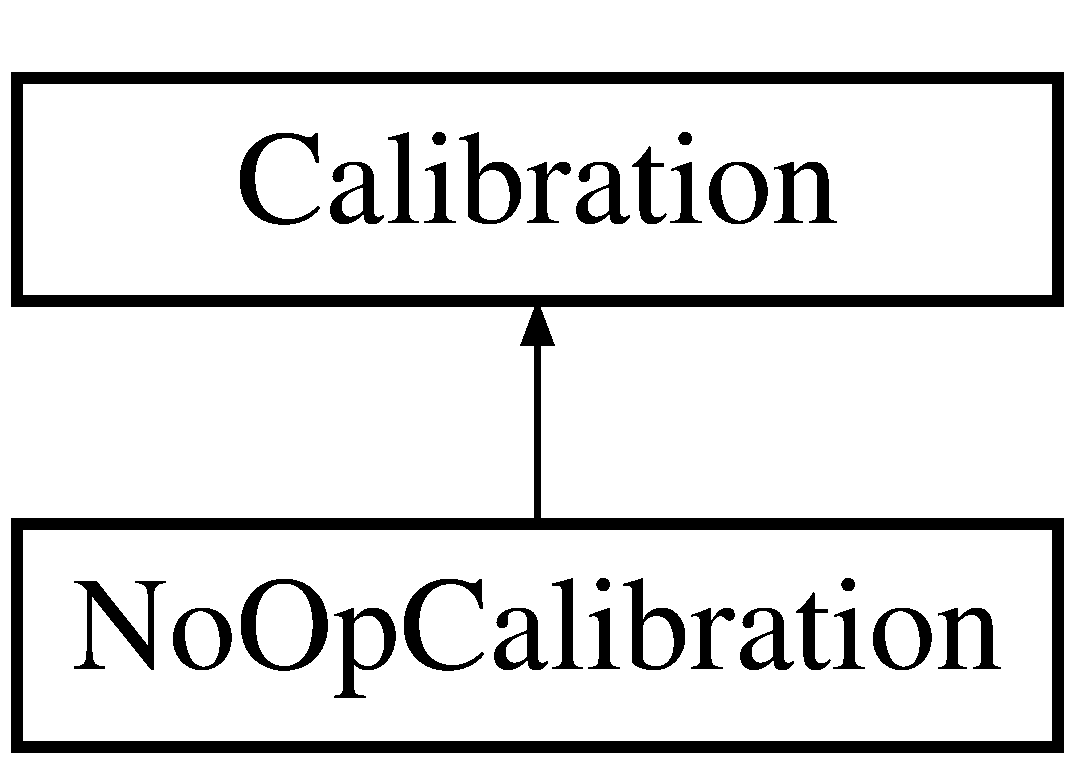
\includegraphics[height=2.000000cm]{classNoOpCalibration}
\end{center}
\end{figure}
\subsection*{Public Member Functions}
\begin{DoxyCompactItemize}
\item 
Float\-\_\-t {\bf get\-Calibrated\-Value} (U\-Int\-\_\-t module\-\_\-index, U\-Int\-\_\-t module\-\_\-type, U\-Int\-\_\-t cell\-\_\-index, Float\-\_\-t adc\-\_\-value) const 
\begin{DoxyCompactList}\small\item\em Determine from a pedestal subtracted A\-D\-C value a calibrated value which are identical for this very lazy calibrator. \end{DoxyCompactList}\item 
Bool\-\_\-t {\bf check\-For\-Calibration\-Constants\-Of\-Module} (U\-Int\-\_\-t module\-\_\-id, U\-Int\-\_\-t module\-\_\-type, U\-Int\-\_\-t n\-\_\-cells) const 
\begin{DoxyCompactList}\small\item\em Verify that calibration constants exist for a certain module. \end{DoxyCompactList}\item 
Int\-\_\-t {\bf get\-Minium\-A\-D\-C\-For\-Mip\-Threshold} (Float\-\_\-t mip\-\_\-energy\-\_\-fraction) const 
\begin{DoxyCompactList}\small\item\em Get the minimum adc value mips will have for the given energy fraction on all pads. \end{DoxyCompactList}\end{DoxyCompactItemize}


\subsection{Detailed Description}
Lazy calibration class. 

Does nothing. 

Definition at line 10 of file No\-Op\-Calibration.\-hh.



\subsection{Member Function Documentation}
\index{No\-Op\-Calibration@{No\-Op\-Calibration}!check\-For\-Calibration\-Constants\-Of\-Module@{check\-For\-Calibration\-Constants\-Of\-Module}}
\index{check\-For\-Calibration\-Constants\-Of\-Module@{check\-For\-Calibration\-Constants\-Of\-Module}!NoOpCalibration@{No\-Op\-Calibration}}
\subsubsection[{check\-For\-Calibration\-Constants\-Of\-Module}]{\setlength{\rightskip}{0pt plus 5cm}Bool\-\_\-t No\-Op\-Calibration\-::check\-For\-Calibration\-Constants\-Of\-Module (
\begin{DoxyParamCaption}
\item[{U\-Int\-\_\-t}]{module\-\_\-id, }
\item[{U\-Int\-\_\-t}]{module\-\_\-type, }
\item[{U\-Int\-\_\-t}]{n\-\_\-cells}
\end{DoxyParamCaption}
) const\hspace{0.3cm}{\ttfamily [inline]}, {\ttfamily [virtual]}}\label{classNoOpCalibration_acdb31ec76cef7720c0cda5fb15ffa2fb}


Verify that calibration constants exist for a certain module. 


\begin{DoxyParams}{Parameters}
{\em module\-\_\-id} & id Or serial number of a module which uniquely identifies a detector module of a certain type. \\
\hline
{\em module\-\_\-type} & the type of the detector module \\
\hline
{\em n\-\_\-cells} & the number of cells on this module. Return true if calibration constants exist for the given module and the number of cells matches the number of calibration constants. \\
\hline
\end{DoxyParams}


Implements {\bf Calibration} \doxyref{}{p.}{classCalibration_a04c8f21c6e77cd3c91c858ca2c9373c4}.



Definition at line 28 of file No\-Op\-Calibration.\-hh.

\index{No\-Op\-Calibration@{No\-Op\-Calibration}!get\-Calibrated\-Value@{get\-Calibrated\-Value}}
\index{get\-Calibrated\-Value@{get\-Calibrated\-Value}!NoOpCalibration@{No\-Op\-Calibration}}
\subsubsection[{get\-Calibrated\-Value}]{\setlength{\rightskip}{0pt plus 5cm}Float\-\_\-t No\-Op\-Calibration\-::get\-Calibrated\-Value (
\begin{DoxyParamCaption}
\item[{U\-Int\-\_\-t}]{module\-\_\-index, }
\item[{U\-Int\-\_\-t}]{module\-\_\-type, }
\item[{U\-Int\-\_\-t}]{cell\-\_\-index, }
\item[{Float\-\_\-t}]{adc\-\_\-value}
\end{DoxyParamCaption}
) const\hspace{0.3cm}{\ttfamily [inline]}, {\ttfamily [virtual]}}\label{classNoOpCalibration_a8dd43819c4e5bb09e097f4db360a57fe}


Determine from a pedestal subtracted A\-D\-C value a calibrated value which are identical for this very lazy calibrator. 


\begin{DoxyParams}{Parameters}
{\em module\-\_\-index} & index of the module a module is considered to be a unit which is always calibrated in one calibration run. \\
\hline
{\em module\-\_\-type} & the type of the detector module \\
\hline
{\em cell\-\_\-index} & \\
\hline
{\em adc\-\_\-value} & the A\-D\-C value which should be calibrated. \\
\hline
\end{DoxyParams}


Implements {\bf Calibration} \doxyref{}{p.}{classCalibration_aca88d93a445ba3021c05dd61b293568c}.



Definition at line 20 of file No\-Op\-Calibration.\-hh.

\index{No\-Op\-Calibration@{No\-Op\-Calibration}!get\-Minium\-A\-D\-C\-For\-Mip\-Threshold@{get\-Minium\-A\-D\-C\-For\-Mip\-Threshold}}
\index{get\-Minium\-A\-D\-C\-For\-Mip\-Threshold@{get\-Minium\-A\-D\-C\-For\-Mip\-Threshold}!NoOpCalibration@{No\-Op\-Calibration}}
\subsubsection[{get\-Minium\-A\-D\-C\-For\-Mip\-Threshold}]{\setlength{\rightskip}{0pt plus 5cm}Int\-\_\-t No\-Op\-Calibration\-::get\-Minium\-A\-D\-C\-For\-Mip\-Threshold (
\begin{DoxyParamCaption}
\item[{Float\-\_\-t}]{mip\-\_\-energy\-\_\-fraction}
\end{DoxyParamCaption}
) const\hspace{0.3cm}{\ttfamily [inline]}, {\ttfamily [virtual]}}\label{classNoOpCalibration_a8b478c6680b5980c2b87cedc8a589989}


Get the minimum adc value mips will have for the given energy fraction on all pads. 


\begin{DoxyParams}{Parameters}
{\em mip\-\_\-energy\-\_\-fraction} & the energy in mips \\
\hline
\end{DoxyParams}
\begin{DoxyReturn}{Returns}
minimum adc value which is below the given energy on all pads. This method can be used to get the lowest adc value a mip of the given energy fraction will have on all pads. This value is useful to select candidates before actually performing th calibration. This function is intended to be called at the beginning of each event. 
\end{DoxyReturn}


Implements {\bf Calibration} \doxyref{}{p.}{classCalibration_a4e45f1eca0d4fdf19ad76b8f581aee12}.



Definition at line 38 of file No\-Op\-Calibration.\-hh.



The documentation for this class was generated from the following file\-:\begin{DoxyCompactItemize}
\item 
No\-Op\-Calibration.\-hh\end{DoxyCompactItemize}

\section{No\-Op\-Calibration\-Kit Class Reference}
\label{classNoOpCalibrationKit}\index{No\-Op\-Calibration\-Kit@{No\-Op\-Calibration\-Kit}}


Create a calibration object which just returns the uncalibrated values.  


Inheritance diagram for No\-Op\-Calibration\-Kit\-:\begin{figure}[H]
\begin{center}
\leavevmode
\includegraphics[height=2.000000cm]{classNoOpCalibrationKit}
\end{center}
\end{figure}
\subsection*{Public Member Functions}
\begin{DoxyCompactItemize}
\item 
{\bf Calibration} $\ast$ {\bf create} (const std\-::string \&module\-\_\-type\-\_\-col\-\_\-name, const std\-::string \&module\-\_\-calibration\-\_\-col\-\_\-name) const 
\begin{DoxyCompactList}\small\item\em create calibration object. \end{DoxyCompactList}\end{DoxyCompactItemize}
\subsection*{Static Protected Attributes}
\begin{DoxyCompactItemize}
\item 
static {\bf No\-Op\-Calibration\-Kit} {\bfseries \-\_\-\-\_\-instance}\label{classNoOpCalibrationKit_a5eb71ed34d9b318427d462277381a6da}

\end{DoxyCompactItemize}


\subsection{Detailed Description}
Create a calibration object which just returns the uncalibrated values. 

\begin{DoxySeeAlso}{See Also}
\doxyref{No\-Op\-Calibration}{p.}{classNoOpCalibration}. 
\end{DoxySeeAlso}


Definition at line 9 of file No\-Op\-Calibration.\-cc.



\subsection{Member Function Documentation}
\index{No\-Op\-Calibration\-Kit@{No\-Op\-Calibration\-Kit}!create@{create}}
\index{create@{create}!NoOpCalibrationKit@{No\-Op\-Calibration\-Kit}}
\subsubsection[{create}]{\setlength{\rightskip}{0pt plus 5cm}{\bf Calibration}$\ast$ No\-Op\-Calibration\-Kit\-::create (
\begin{DoxyParamCaption}
\item[{const std\-::string \&}]{module\-\_\-type\-\_\-col\-\_\-name, }
\item[{const std\-::string \&}]{module\-\_\-calibration\-\_\-col\-\_\-name}
\end{DoxyParamCaption}
) const\hspace{0.3cm}{\ttfamily [inline]}, {\ttfamily [virtual]}}\label{classNoOpCalibrationKit_ac197f7bf5528b484d5b70e664655474b}


create calibration object. 


\begin{DoxyParams}{Parameters}
{\em module\-\_\-type\-\_\-col\-\_\-name} & the name of the conditions data collection with the module types. \\
\hline
{\em module\-\_\-calibration\-\_\-col\-\_\-name} & the name of the conditions data collection which contains the calibration constants. F\-I\-X\-M\-E\-: There should be a better method to hand parameters to \doxyref{Calibration}{p.}{classCalibration} objects. \\
\hline
\end{DoxyParams}


Implements {\bf Calibration\-Kit} \doxyref{}{p.}{classCalibrationKit_ab3aea5671d91a7b6f5e839324cf45a70}.



Definition at line 20 of file No\-Op\-Calibration.\-cc.



The documentation for this class was generated from the following file\-:\begin{DoxyCompactItemize}
\item 
No\-Op\-Calibration.\-cc\end{DoxyCompactItemize}

\section{C\-A\-L\-I\-C\-E\-:\-:N\-Vector\-\_\-t$<$ T, dimension $>$ Class Template Reference}
\label{classCALICE_1_1NVector__t}\index{C\-A\-L\-I\-C\-E\-::\-N\-Vector\-\_\-t$<$ T, dimension $>$@{C\-A\-L\-I\-C\-E\-::\-N\-Vector\-\_\-t$<$ T, dimension $>$}}


Simple n-\/dimensional vector (size of the vector is defined at compile time) Provides methods to add and subtract vectors or multiply and divide by scalars.  




{\ttfamily \#include $<$N\-Vector\-\_\-t.\-hh$>$}

\subsection*{Public Member Functions}
\begin{DoxyCompactItemize}
\item 
{\bf N\-Vector\-\_\-t} \& {\bf clear} ()
\begin{DoxyCompactList}\small\item\em Set all elements to zero. \end{DoxyCompactList}\item 
U\-Int\-\_\-t {\bf n} () const \label{classCALICE_1_1NVector__t_abdf25cc48054ab30cf01c410f8e8279a}

\begin{DoxyCompactList}\small\item\em Get the dimension of the vector. \end{DoxyCompactList}\item 
{\bf N\-Vector\-\_\-t} \& {\bf set} (const T $\ast$array)
\begin{DoxyCompactList}\small\item\em Set the elements of the vector from the given array. \end{DoxyCompactList}\item 
Float\-\_\-t \& {\bf operator[$\,$]} (U\-Int\-\_\-t index)
\begin{DoxyCompactList}\small\item\em get the element of the given index (read and write access). \end{DoxyCompactList}\item 
const Float\-\_\-t \& {\bf operator[$\,$]} (U\-Int\-\_\-t index) const 
\begin{DoxyCompactList}\small\item\em get the element of the given index (read access only). \end{DoxyCompactList}\item 
{\bf N\-Vector\-\_\-t} \& {\bf operator+=} (const {\bf N\-Vector\-\_\-t} \&a)
\begin{DoxyCompactList}\small\item\em Add a vector having the same dimension to this vector. \end{DoxyCompactList}\item 
{\bf N\-Vector\-\_\-t} \& {\bf operator-\/=} (const {\bf N\-Vector\-\_\-t} \&a)
\begin{DoxyCompactList}\small\item\em Subtract a vector having the same dimension to this vector. \end{DoxyCompactList}\item 
{\bf N\-Vector\-\_\-t} \& {\bf operator$\ast$=} (const float c)
\begin{DoxyCompactList}\small\item\em Multiply this vector by a scalar. \end{DoxyCompactList}\item 
{\bf N\-Vector\-\_\-t} \& {\bf operator/=} (const float c)
\begin{DoxyCompactList}\small\item\em Divide this vector by a scalar. \end{DoxyCompactList}\item 
Float\-\_\-t $\ast$ {\bf data} ()
\begin{DoxyCompactList}\small\item\em get a pointer to the underlying array (read and write access). \end{DoxyCompactList}\item 
const Float\-\_\-t $\ast$ {\bf data} () const 
\begin{DoxyCompactList}\small\item\em get a pointer to the underlying array (read only access). \end{DoxyCompactList}\end{DoxyCompactItemize}
\subsection*{Private Attributes}
\begin{DoxyCompactItemize}
\item 
Float\-\_\-t {\bf \-\_\-x} [dimension]
\end{DoxyCompactItemize}
\subsection*{Friends}
\begin{DoxyCompactItemize}
\item 
{\footnotesize template$<$class \-\_\-\-T , int \-\_\-dimension$>$ }\\{\bf N\-Vector\-\_\-t}$<$ \-\_\-\-T, \-\_\-dimension $>$ {\bf operator-\/} (const {\bf N\-Vector\-\_\-t}$<$ \-\_\-\-T, \-\_\-dimension $>$ \&a, const {\bf N\-Vector\-\_\-t}$<$ \-\_\-\-T, \-\_\-dimension $>$ \&b)\label{classCALICE_1_1NVector__t_a8b9a92a937c2f74d6a98889be55373db}

\begin{DoxyCompactList}\small\item\em Subtract two vectors of the same dimension. \end{DoxyCompactList}\item 
{\footnotesize template$<$class \-\_\-\-T , int \-\_\-dimension$>$ }\\{\bf N\-Vector\-\_\-t}$<$ \-\_\-\-T, \-\_\-dimension $>$ {\bf operator+} (const {\bf N\-Vector\-\_\-t}$<$ \-\_\-\-T, \-\_\-dimension $>$ \&a, const {\bf N\-Vector\-\_\-t}$<$ \-\_\-\-T, \-\_\-dimension $>$ \&b)\label{classCALICE_1_1NVector__t_a345dbcc20a67386011969dccac6ed891}

\begin{DoxyCompactList}\small\item\em Add two vectors of the same dimension. \end{DoxyCompactList}\item 
{\footnotesize template$<$class \-\_\-\-T , int \-\_\-dimension$>$ }\\{\bf N\-Vector\-\_\-t}$<$ \-\_\-\-T, \-\_\-dimension $>$ {\bf operator$\ast$} (const {\bf N\-Vector\-\_\-t}$<$ \-\_\-\-T, \-\_\-dimension $>$ \&a, float c)
\begin{DoxyCompactList}\small\item\em Multiply a vector by a scalar. \end{DoxyCompactList}\item 
{\footnotesize template$<$class \-\_\-\-T , int \-\_\-dimension$>$ }\\{\bf N\-Vector\-\_\-t}$<$ \-\_\-\-T, \-\_\-dimension $>$ {\bf operator$\ast$} (float c, const {\bf N\-Vector\-\_\-t}$<$ \-\_\-\-T, \-\_\-dimension $>$ \&a)
\begin{DoxyCompactList}\small\item\em Multiply a vector by a scalar. \end{DoxyCompactList}\item 
{\footnotesize template$<$class \-\_\-\-T , int \-\_\-dimension$>$ }\\{\bf N\-Vector\-\_\-t}$<$ \-\_\-\-T, \-\_\-dimension $>$ {\bf operator/} (const {\bf N\-Vector\-\_\-t}$<$ \-\_\-\-T, \-\_\-dimension $>$ \&a, float c)
\begin{DoxyCompactList}\small\item\em Divide a vector by a scalar. \end{DoxyCompactList}\item 
{\footnotesize template$<$class \-\_\-\-T , int \-\_\-dimension$>$ }\\Double\-\_\-t {\bf norm} (const {\bf N\-Vector\-\_\-t}$<$ \-\_\-\-T, \-\_\-dimension $>$ \&a)\label{classCALICE_1_1NVector__t_abc603727f3464e21addcc6dfcad55953}

\begin{DoxyCompactList}\small\item\em Euclidean Norm of a vector. \end{DoxyCompactList}\item 
{\footnotesize template$<$class \-\_\-\-T , int \-\_\-dimension$>$ }\\Double\-\_\-t {\bf dot} (const {\bf N\-Vector\-\_\-t}$<$ \-\_\-\-T, \-\_\-dimension $>$ \&a, const {\bf N\-Vector\-\_\-t}$<$ \-\_\-\-T, \-\_\-dimension $>$ \&b)\label{classCALICE_1_1NVector__t_a4e03d5cfcb4cd45a83308d7218af8ac2}

\begin{DoxyCompactList}\small\item\em Scalar product of two vectors of the same dimension. \end{DoxyCompactList}\item 
{\bf Three\-Vector\-\_\-t} {\bf cross} (const {\bf Three\-Vector\-\_\-t} \&a, const {\bf Three\-Vector\-\_\-t} \&b)\label{classCALICE_1_1NVector__t_a4cad467a11b3438c7bc1afc3995ae2cb}

\begin{DoxyCompactList}\small\item\em cross product of two three dimensional vectors. \end{DoxyCompactList}\end{DoxyCompactItemize}


\subsection{Detailed Description}
\subsubsection*{template$<$class T, int dimension$>$class C\-A\-L\-I\-C\-E\-::\-N\-Vector\-\_\-t$<$ T, dimension $>$}

Simple n-\/dimensional vector (size of the vector is defined at compile time) Provides methods to add and subtract vectors or multiply and divide by scalars. 

There are also functions to calculate the scalar and cross products (the latter for three dimensional vectors only). A flat array (currently floats only) can be casted to an \doxyref{N\-Vector\-\_\-t}{p.}{classCALICE_1_1NVector__t}\-: {\ttfamily  lcio\-::\-Calorimeter\-Hit $\ast$a\-\_\-hit; N\-Vector\-\_\-t$<$\-Float\-\_\-t,3$>$ $\ast$vector=static\-\_\-cast$<$N\-Vector\-\_\-t$<$\-Float\-\_\-t,3$>$ $\ast$$>$(a\-\_\-hit-\/$>$get\-Position()); } 

Definition at line 12 of file N\-Vector\-\_\-t.\-hh.



\subsection{Member Function Documentation}
\index{C\-A\-L\-I\-C\-E\-::\-N\-Vector\-\_\-t@{C\-A\-L\-I\-C\-E\-::\-N\-Vector\-\_\-t}!clear@{clear}}
\index{clear@{clear}!CALICE::NVector_t@{C\-A\-L\-I\-C\-E\-::\-N\-Vector\-\_\-t}}
\subsubsection[{clear}]{\setlength{\rightskip}{0pt plus 5cm}template$<$class T, int dimension$>$ {\bf N\-Vector\-\_\-t}\& {\bf C\-A\-L\-I\-C\-E\-::\-N\-Vector\-\_\-t}$<$ T, dimension $>$\-::clear (
\begin{DoxyParamCaption}
{}
\end{DoxyParamCaption}
)\hspace{0.3cm}{\ttfamily [inline]}}\label{classCALICE_1_1NVector__t_acdcc0e98ea504c04cfc4341269969e5c}


Set all elements to zero. 

\begin{DoxyRefDesc}{Todo}
\item[{\bf Todo}]this only works for simple types like int, float, double. \end{DoxyRefDesc}


Definition at line 45 of file N\-Vector\-\_\-t.\-hh.



References C\-A\-L\-I\-C\-E\-::\-N\-Vector\-\_\-t$<$ T, dimension $>$\-::\-\_\-x.

\index{C\-A\-L\-I\-C\-E\-::\-N\-Vector\-\_\-t@{C\-A\-L\-I\-C\-E\-::\-N\-Vector\-\_\-t}!data@{data}}
\index{data@{data}!CALICE::NVector_t@{C\-A\-L\-I\-C\-E\-::\-N\-Vector\-\_\-t}}
\subsubsection[{data}]{\setlength{\rightskip}{0pt plus 5cm}template$<$class T, int dimension$>$ Float\-\_\-t$\ast$ {\bf C\-A\-L\-I\-C\-E\-::\-N\-Vector\-\_\-t}$<$ T, dimension $>$\-::data (
\begin{DoxyParamCaption}
{}
\end{DoxyParamCaption}
)\hspace{0.3cm}{\ttfamily [inline]}}\label{classCALICE_1_1NVector__t_a216c4f7afc34c21e101a4122e857a120}


get a pointer to the underlying array (read and write access). 



Definition at line 139 of file N\-Vector\-\_\-t.\-hh.



References C\-A\-L\-I\-C\-E\-::\-N\-Vector\-\_\-t$<$ T, dimension $>$\-::\-\_\-x.

\index{C\-A\-L\-I\-C\-E\-::\-N\-Vector\-\_\-t@{C\-A\-L\-I\-C\-E\-::\-N\-Vector\-\_\-t}!data@{data}}
\index{data@{data}!CALICE::NVector_t@{C\-A\-L\-I\-C\-E\-::\-N\-Vector\-\_\-t}}
\subsubsection[{data}]{\setlength{\rightskip}{0pt plus 5cm}template$<$class T, int dimension$>$ const Float\-\_\-t$\ast$ {\bf C\-A\-L\-I\-C\-E\-::\-N\-Vector\-\_\-t}$<$ T, dimension $>$\-::data (
\begin{DoxyParamCaption}
{}
\end{DoxyParamCaption}
) const\hspace{0.3cm}{\ttfamily [inline]}}\label{classCALICE_1_1NVector__t_ad523fba7620726c1d58a5b32c8b2d517}


get a pointer to the underlying array (read only access). 

\begin{DoxyRefDesc}{Todo}
\item[{\bf Todo}]float ? not T ? \end{DoxyRefDesc}


Definition at line 142 of file N\-Vector\-\_\-t.\-hh.



References C\-A\-L\-I\-C\-E\-::\-N\-Vector\-\_\-t$<$ T, dimension $>$\-::\-\_\-x.

\index{C\-A\-L\-I\-C\-E\-::\-N\-Vector\-\_\-t@{C\-A\-L\-I\-C\-E\-::\-N\-Vector\-\_\-t}!operator$\ast$=@{operator$\ast$=}}
\index{operator$\ast$=@{operator$\ast$=}!CALICE::NVector_t@{C\-A\-L\-I\-C\-E\-::\-N\-Vector\-\_\-t}}
\subsubsection[{operator$\ast$=}]{\setlength{\rightskip}{0pt plus 5cm}template$<$class T, int dimension$>$ {\bf N\-Vector\-\_\-t}\& {\bf C\-A\-L\-I\-C\-E\-::\-N\-Vector\-\_\-t}$<$ T, dimension $>$\-::operator$\ast$= (
\begin{DoxyParamCaption}
\item[{const float}]{c}
\end{DoxyParamCaption}
)\hspace{0.3cm}{\ttfamily [inline]}}\label{classCALICE_1_1NVector__t_af177ac27d671789ac8c8d61f257ccd4b}


Multiply this vector by a scalar. 

\begin{DoxyRefDesc}{Todo}
\item[{\bf Todo}]the argument should not be a float but T ? \end{DoxyRefDesc}


Definition at line 125 of file N\-Vector\-\_\-t.\-hh.



References C\-A\-L\-I\-C\-E\-::\-N\-Vector\-\_\-t$<$ T, dimension $>$\-::\-\_\-x.

\index{C\-A\-L\-I\-C\-E\-::\-N\-Vector\-\_\-t@{C\-A\-L\-I\-C\-E\-::\-N\-Vector\-\_\-t}!operator+=@{operator+=}}
\index{operator+=@{operator+=}!CALICE::NVector_t@{C\-A\-L\-I\-C\-E\-::\-N\-Vector\-\_\-t}}
\subsubsection[{operator+=}]{\setlength{\rightskip}{0pt plus 5cm}template$<$class T, int dimension$>$ {\bf N\-Vector\-\_\-t}\& {\bf C\-A\-L\-I\-C\-E\-::\-N\-Vector\-\_\-t}$<$ T, dimension $>$\-::operator+= (
\begin{DoxyParamCaption}
\item[{const {\bf N\-Vector\-\_\-t}$<$ T, dimension $>$ \&}]{a}
\end{DoxyParamCaption}
)\hspace{0.3cm}{\ttfamily [inline]}}\label{classCALICE_1_1NVector__t_ab2f2ef8cb2e16956a24eafcfd5965b19}


Add a vector having the same dimension to this vector. 

F\-I\-X\-M\-E\-: The compiler should create an error message if vectors of different dimensions are added Does this happen ? 

Definition at line 108 of file N\-Vector\-\_\-t.\-hh.



References C\-A\-L\-I\-C\-E\-::\-N\-Vector\-\_\-t$<$ T, dimension $>$\-::\-\_\-x.

\index{C\-A\-L\-I\-C\-E\-::\-N\-Vector\-\_\-t@{C\-A\-L\-I\-C\-E\-::\-N\-Vector\-\_\-t}!operator-\/=@{operator-\/=}}
\index{operator-\/=@{operator-\/=}!CALICE::NVector_t@{C\-A\-L\-I\-C\-E\-::\-N\-Vector\-\_\-t}}
\subsubsection[{operator-\/=}]{\setlength{\rightskip}{0pt plus 5cm}template$<$class T, int dimension$>$ {\bf N\-Vector\-\_\-t}\& {\bf C\-A\-L\-I\-C\-E\-::\-N\-Vector\-\_\-t}$<$ T, dimension $>$\-::operator-\/= (
\begin{DoxyParamCaption}
\item[{const {\bf N\-Vector\-\_\-t}$<$ T, dimension $>$ \&}]{a}
\end{DoxyParamCaption}
)\hspace{0.3cm}{\ttfamily [inline]}}\label{classCALICE_1_1NVector__t_a921fef3e1b5fe52897c80917a696614d}


Subtract a vector having the same dimension to this vector. 

F\-I\-X\-M\-E\-: The compiler should create an error message if vectors of different dimensions are added Does this happen ? 

Definition at line 117 of file N\-Vector\-\_\-t.\-hh.



References C\-A\-L\-I\-C\-E\-::\-N\-Vector\-\_\-t$<$ T, dimension $>$\-::\-\_\-x.

\index{C\-A\-L\-I\-C\-E\-::\-N\-Vector\-\_\-t@{C\-A\-L\-I\-C\-E\-::\-N\-Vector\-\_\-t}!operator/=@{operator/=}}
\index{operator/=@{operator/=}!CALICE::NVector_t@{C\-A\-L\-I\-C\-E\-::\-N\-Vector\-\_\-t}}
\subsubsection[{operator/=}]{\setlength{\rightskip}{0pt plus 5cm}template$<$class T, int dimension$>$ {\bf N\-Vector\-\_\-t}\& {\bf C\-A\-L\-I\-C\-E\-::\-N\-Vector\-\_\-t}$<$ T, dimension $>$\-::operator/= (
\begin{DoxyParamCaption}
\item[{const float}]{c}
\end{DoxyParamCaption}
)\hspace{0.3cm}{\ttfamily [inline]}}\label{classCALICE_1_1NVector__t_ab9758bc6c1ae323e33d25457b1f60993}


Divide this vector by a scalar. 

\begin{DoxyRefDesc}{Todo}
\item[{\bf Todo}]the argument should not be a float but T ? \end{DoxyRefDesc}


Definition at line 133 of file N\-Vector\-\_\-t.\-hh.



References C\-A\-L\-I\-C\-E\-::\-N\-Vector\-\_\-t$<$ T, dimension $>$\-::\-\_\-x.

\index{C\-A\-L\-I\-C\-E\-::\-N\-Vector\-\_\-t@{C\-A\-L\-I\-C\-E\-::\-N\-Vector\-\_\-t}!operator[$\,$]@{operator[]}}
\index{operator[$\,$]@{operator[]}!CALICE::NVector_t@{C\-A\-L\-I\-C\-E\-::\-N\-Vector\-\_\-t}}
\subsubsection[{operator[]}]{\setlength{\rightskip}{0pt plus 5cm}template$<$class T, int dimension$>$ Float\-\_\-t\& {\bf C\-A\-L\-I\-C\-E\-::\-N\-Vector\-\_\-t}$<$ T, dimension $>$\-::operator[$\,$] (
\begin{DoxyParamCaption}
\item[{U\-Int\-\_\-t}]{index}
\end{DoxyParamCaption}
)\hspace{0.3cm}{\ttfamily [inline]}}\label{classCALICE_1_1NVector__t_aa001e473489cb79a2be6bb0708b5f9be}


get the element of the given index (read and write access). 


\begin{DoxyParams}{Parameters}
{\em index} & the index of the element (0 to dimension -\/ 1). \\
\hline
\end{DoxyParams}
\begin{DoxyReturn}{Returns}
reference to the element of the given index (read and write access). When the preprocessor variable B\-O\-U\-N\-D\-A\-R\-Y\-\_\-\-C\-H\-E\-C\-K is defined the validity of index is checked and an exception std\-::runtime\-\_\-error is thrown in case of violations. 
\end{DoxyReturn}


Definition at line 71 of file N\-Vector\-\_\-t.\-hh.



References C\-A\-L\-I\-C\-E\-::\-N\-Vector\-\_\-t$<$ T, dimension $>$\-::\-\_\-x.

\index{C\-A\-L\-I\-C\-E\-::\-N\-Vector\-\_\-t@{C\-A\-L\-I\-C\-E\-::\-N\-Vector\-\_\-t}!operator[$\,$]@{operator[]}}
\index{operator[$\,$]@{operator[]}!CALICE::NVector_t@{C\-A\-L\-I\-C\-E\-::\-N\-Vector\-\_\-t}}
\subsubsection[{operator[]}]{\setlength{\rightskip}{0pt plus 5cm}template$<$class T, int dimension$>$ const Float\-\_\-t\& {\bf C\-A\-L\-I\-C\-E\-::\-N\-Vector\-\_\-t}$<$ T, dimension $>$\-::operator[$\,$] (
\begin{DoxyParamCaption}
\item[{U\-Int\-\_\-t}]{index}
\end{DoxyParamCaption}
) const\hspace{0.3cm}{\ttfamily [inline]}}\label{classCALICE_1_1NVector__t_afb5ddce261165c101329cba31be6363b}


get the element of the given index (read access only). 


\begin{DoxyParams}{Parameters}
{\em index} & the index of the element (0 to dimension -\/ 1). \\
\hline
\end{DoxyParams}
\begin{DoxyReturn}{Returns}
reference to the element of the given index (read access only). When the preprocessor variable B\-O\-U\-N\-D\-A\-R\-Y\-\_\-\-C\-H\-E\-C\-K is defined the validity of index is checked and an exception std\-::runtime\-\_\-error is thrown in case of violations. 
\end{DoxyReturn}


Definition at line 91 of file N\-Vector\-\_\-t.\-hh.



References C\-A\-L\-I\-C\-E\-::\-N\-Vector\-\_\-t$<$ T, dimension $>$\-::\-\_\-x.

\index{C\-A\-L\-I\-C\-E\-::\-N\-Vector\-\_\-t@{C\-A\-L\-I\-C\-E\-::\-N\-Vector\-\_\-t}!set@{set}}
\index{set@{set}!CALICE::NVector_t@{C\-A\-L\-I\-C\-E\-::\-N\-Vector\-\_\-t}}
\subsubsection[{set}]{\setlength{\rightskip}{0pt plus 5cm}template$<$class T, int dimension$>$ {\bf N\-Vector\-\_\-t}\& {\bf C\-A\-L\-I\-C\-E\-::\-N\-Vector\-\_\-t}$<$ T, dimension $>$\-::set (
\begin{DoxyParamCaption}
\item[{const T $\ast$}]{array}
\end{DoxyParamCaption}
)\hspace{0.3cm}{\ttfamily [inline]}}\label{classCALICE_1_1NVector__t_a72e8589546f57d77aa0368c56f1b9824}


Set the elements of the vector from the given array. 

It is assumed that the array contains the correct amount of elements (dimension of the vector). If the dimension of the given array is smaller than the dimension of this vector then the result will be undefined. 

Definition at line 59 of file N\-Vector\-\_\-t.\-hh.



References C\-A\-L\-I\-C\-E\-::\-N\-Vector\-\_\-t$<$ T, dimension $>$\-::\-\_\-x.



\subsection{Friends And Related Function Documentation}
\index{C\-A\-L\-I\-C\-E\-::\-N\-Vector\-\_\-t@{C\-A\-L\-I\-C\-E\-::\-N\-Vector\-\_\-t}!operator$\ast$@{operator$\ast$}}
\index{operator$\ast$@{operator$\ast$}!CALICE::NVector_t@{C\-A\-L\-I\-C\-E\-::\-N\-Vector\-\_\-t}}
\subsubsection[{operator$\ast$}]{\setlength{\rightskip}{0pt plus 5cm}template$<$class T, int dimension$>$ template$<$class \-\_\-\-T , int \-\_\-dimension$>$ {\bf N\-Vector\-\_\-t}$<$\-\_\-\-T,\-\_\-dimension$>$ operator$\ast$ (
\begin{DoxyParamCaption}
\item[{const {\bf N\-Vector\-\_\-t}$<$ \-\_\-\-T, \-\_\-dimension $>$ \&}]{a, }
\item[{float}]{c}
\end{DoxyParamCaption}
)\hspace{0.3cm}{\ttfamily [friend]}}\label{classCALICE_1_1NVector__t_a05383138d229b2507e6903656ee16148}


Multiply a vector by a scalar. 

\begin{DoxyRefDesc}{Todo}
\item[{\bf Todo}]replace float by \-\_\-\-T? \end{DoxyRefDesc}


Definition at line 182 of file N\-Vector\-\_\-t.\-hh.

\index{C\-A\-L\-I\-C\-E\-::\-N\-Vector\-\_\-t@{C\-A\-L\-I\-C\-E\-::\-N\-Vector\-\_\-t}!operator$\ast$@{operator$\ast$}}
\index{operator$\ast$@{operator$\ast$}!CALICE::NVector_t@{C\-A\-L\-I\-C\-E\-::\-N\-Vector\-\_\-t}}
\subsubsection[{operator$\ast$}]{\setlength{\rightskip}{0pt plus 5cm}template$<$class T, int dimension$>$ template$<$class \-\_\-\-T , int \-\_\-dimension$>$ {\bf N\-Vector\-\_\-t}$<$\-\_\-\-T,\-\_\-dimension$>$ operator$\ast$ (
\begin{DoxyParamCaption}
\item[{float}]{c, }
\item[{const {\bf N\-Vector\-\_\-t}$<$ \-\_\-\-T, \-\_\-dimension $>$ \&}]{a}
\end{DoxyParamCaption}
)\hspace{0.3cm}{\ttfamily [friend]}}\label{classCALICE_1_1NVector__t_a0bb45733b94281bb1d1c77ad9675ed7e}


Multiply a vector by a scalar. 

\begin{DoxyRefDesc}{Todo}
\item[{\bf Todo}]replace float by \-\_\-\-T? \end{DoxyRefDesc}


Definition at line 171 of file N\-Vector\-\_\-t.\-hh.

\index{C\-A\-L\-I\-C\-E\-::\-N\-Vector\-\_\-t@{C\-A\-L\-I\-C\-E\-::\-N\-Vector\-\_\-t}!operator/@{operator/}}
\index{operator/@{operator/}!CALICE::NVector_t@{C\-A\-L\-I\-C\-E\-::\-N\-Vector\-\_\-t}}
\subsubsection[{operator/}]{\setlength{\rightskip}{0pt plus 5cm}template$<$class T, int dimension$>$ template$<$class \-\_\-\-T , int \-\_\-dimension$>$ {\bf N\-Vector\-\_\-t}$<$\-\_\-\-T,\-\_\-dimension$>$ operator/ (
\begin{DoxyParamCaption}
\item[{const {\bf N\-Vector\-\_\-t}$<$ \-\_\-\-T, \-\_\-dimension $>$ \&}]{a, }
\item[{float}]{c}
\end{DoxyParamCaption}
)\hspace{0.3cm}{\ttfamily [friend]}}\label{classCALICE_1_1NVector__t_a3fb7ccd2a9a60442a2c0a6f1c53dd7d0}


Divide a vector by a scalar. 

\begin{DoxyRefDesc}{Todo}
\item[{\bf Todo}]replace float by \-\_\-\-T? \end{DoxyRefDesc}


Definition at line 193 of file N\-Vector\-\_\-t.\-hh.



\subsection{Field Documentation}
\index{C\-A\-L\-I\-C\-E\-::\-N\-Vector\-\_\-t@{C\-A\-L\-I\-C\-E\-::\-N\-Vector\-\_\-t}!\-\_\-x@{\-\_\-x}}
\index{\-\_\-x@{\-\_\-x}!CALICE::NVector_t@{C\-A\-L\-I\-C\-E\-::\-N\-Vector\-\_\-t}}
\subsubsection[{\-\_\-x}]{\setlength{\rightskip}{0pt plus 5cm}template$<$class T, int dimension$>$ Float\-\_\-t {\bf C\-A\-L\-I\-C\-E\-::\-N\-Vector\-\_\-t}$<$ T, dimension $>$\-::\-\_\-x[dimension]\hspace{0.3cm}{\ttfamily [private]}}\label{classCALICE_1_1NVector__t_a8089ceb5c1305789d489631c1da4913c}
\begin{DoxyRefDesc}{Todo}
\item[{\bf Todo}]float ? not T ? \end{DoxyRefDesc}
\begin{DoxyRefDesc}{Todo}
\item[{\bf Todo}]float ? not T ? \end{DoxyRefDesc}


Definition at line 142 of file N\-Vector\-\_\-t.\-hh.



Referenced by C\-A\-L\-I\-C\-E\-::\-N\-Vector\-\_\-t$<$ T, dimension $>$\-::clear(), C\-A\-L\-I\-C\-E\-::cross(), C\-A\-L\-I\-C\-E\-::\-N\-Vector\-\_\-t$<$ T, dimension $>$\-::data(), C\-A\-L\-I\-C\-E\-::dot(), C\-A\-L\-I\-C\-E\-::norm(), C\-A\-L\-I\-C\-E\-::operator$\ast$(), C\-A\-L\-I\-C\-E\-::\-N\-Vector\-\_\-t$<$ T, dimension $>$\-::operator$\ast$=(), C\-A\-L\-I\-C\-E\-::operator+(), C\-A\-L\-I\-C\-E\-::\-N\-Vector\-\_\-t$<$ T, dimension $>$\-::operator+=(), C\-A\-L\-I\-C\-E\-::operator-\/(), C\-A\-L\-I\-C\-E\-::\-N\-Vector\-\_\-t$<$ T, dimension $>$\-::operator-\/=(), C\-A\-L\-I\-C\-E\-::operator/(), C\-A\-L\-I\-C\-E\-::\-N\-Vector\-\_\-t$<$ T, dimension $>$\-::operator/=(), C\-A\-L\-I\-C\-E\-::\-N\-Vector\-\_\-t$<$ T, dimension $>$\-::operator[$\,$](), and C\-A\-L\-I\-C\-E\-::\-N\-Vector\-\_\-t$<$ T, dimension $>$\-::set().



The documentation for this class was generated from the following file\-:\begin{DoxyCompactItemize}
\item 
N\-Vector\-\_\-t.\-hh\end{DoxyCompactItemize}

\section{C\-A\-L\-I\-C\-E\-:\-:Pedestal\-Noise\-Histograms Class Reference}
\label{classCALICE_1_1PedestalNoiseHistograms}\index{C\-A\-L\-I\-C\-E\-::\-Pedestal\-Noise\-Histograms@{C\-A\-L\-I\-C\-E\-::\-Pedestal\-Noise\-Histograms}}
Inheritance diagram for C\-A\-L\-I\-C\-E\-:\-:Pedestal\-Noise\-Histograms\-:\begin{figure}[H]
\begin{center}
\leavevmode
\includegraphics[height=3.000000cm]{classCALICE_1_1PedestalNoiseHistograms}
\end{center}
\end{figure}
\subsection*{Public Member Functions}
\begin{DoxyCompactItemize}
\item 
Processor $\ast$ {\bfseries new\-Processor} ()\label{classCALICE_1_1PedestalNoiseHistograms_ae5a513bca3d9c3fa642c3006723a3c40}

\item 
void {\bf init} ()
\begin{DoxyCompactList}\small\item\em Called at the begin of the job before anything is read. \end{DoxyCompactList}\item 
void {\bf process\-Run\-Header} (L\-C\-Run\-Header $\ast$run)
\begin{DoxyCompactList}\small\item\em Called for every run, e.\-g. \end{DoxyCompactList}\item 
void {\bf process\-Event} (L\-C\-Event $\ast$evt\-P)
\begin{DoxyCompactList}\small\item\em Called for every event -\/ the working horse. \end{DoxyCompactList}\item 
void {\bfseries end} ()\label{classCALICE_1_1PedestalNoiseHistograms_a0b92f798c4e9e32ffb7e938136db8e20}

\end{DoxyCompactItemize}
\subsection*{Protected Types}
\begin{DoxyCompactItemize}
\item 
enum {\bfseries E\-H1\-Type} \{ {\bfseries k\-H1\-Noise}, 
{\bfseries k\-H1\-Pedestal}, 
{\bfseries k\-N\-H1}
 \}
\end{DoxyCompactItemize}
\subsection*{Protected Member Functions}
\begin{DoxyCompactItemize}
\item 
void {\bfseries module\-Type\-Changed} (lcio\-::\-L\-C\-Collection $\ast$col)\label{classCALICE_1_1PedestalNoiseHistograms_a2e3c07637bf5c56983d397633da2088c}

\item 
void {\bfseries module\-Location\-Changed} (lcio\-::\-L\-C\-Collection $\ast$col)\label{classCALICE_1_1PedestalNoiseHistograms_a19422319fb37675b47ed8b75c751c518}

\item 
void {\bfseries module\-Connection\-Changed} (lcio\-::\-L\-C\-Collection $\ast$col)\label{classCALICE_1_1PedestalNoiseHistograms_a45a6819f1ecd53413ea4c3384130f956}

\item 
void {\bfseries detector\-Changed} ()\label{classCALICE_1_1PedestalNoiseHistograms_a9c381457a97f7d6a5719c106cfe22470}

\item 
void {\bfseries create\-Histograms} ()\label{classCALICE_1_1PedestalNoiseHistograms_a12ca8d443b6eaaaabdf30d6ab744cd77}

\end{DoxyCompactItemize}
\subsection*{Protected Attributes}
\begin{DoxyCompactItemize}
\item 
std\-::string {\bfseries \-\_\-cell\-Parameter\-Collection\-Name}\label{classCALICE_1_1PedestalNoiseHistograms_abaadb2fa0bbd710ae117f584641b8fdb}

\item 
Int\-Vec {\bfseries \-\_\-event\-Par}\label{classCALICE_1_1PedestalNoiseHistograms_ae861039b81067ae12a5dea74318f8435}

\item 
{\bf histmgr\-::\-Key\-\_\-t} {\bfseries \-\_\-histogram\-Group\-Key}\label{classCALICE_1_1PedestalNoiseHistograms_af57634693e902aa26716096d357796fe}

\item 
lcio\-::\-Float\-Vec {\bfseries \-\_\-noise\-Hist\-Par}\label{classCALICE_1_1PedestalNoiseHistograms_a5e6e5886b0245d89be77ccc0f116fecb}

\item 
lcio\-::\-Float\-Vec {\bfseries \-\_\-adc\-Hist\-Par}\label{classCALICE_1_1PedestalNoiseHistograms_a79d98a735280c78211ffcb464cd1173a}

\item 
{\bf histmgr\-::\-Key\-\_\-t} {\bfseries \-\_\-hist\-Key} [k\-N\-H1]\label{classCALICE_1_1PedestalNoiseHistograms_a24c5e21337d538e38f8f53d1219bdd91}

\item 
U\-Int\-\_\-t {\bfseries \-\_\-missing\-Cell\-Parameters}\label{classCALICE_1_1PedestalNoiseHistograms_a6e32fc4df33029b95b827bbee5700046}

\end{DoxyCompactItemize}


\subsection{Detailed Description}


Definition at line 14 of file Pedestal\-Noise\-Histograms.\-hh.



\subsection{Member Function Documentation}
\index{C\-A\-L\-I\-C\-E\-::\-Pedestal\-Noise\-Histograms@{C\-A\-L\-I\-C\-E\-::\-Pedestal\-Noise\-Histograms}!init@{init}}
\index{init@{init}!CALICE::PedestalNoiseHistograms@{C\-A\-L\-I\-C\-E\-::\-Pedestal\-Noise\-Histograms}}
\subsubsection[{init}]{\setlength{\rightskip}{0pt plus 5cm}void C\-A\-L\-I\-C\-E\-::\-Pedestal\-Noise\-Histograms\-::init (
\begin{DoxyParamCaption}
{}
\end{DoxyParamCaption}
)}\label{classCALICE_1_1PedestalNoiseHistograms_a1558ef3262c57736081abced8094309e}


Called at the begin of the job before anything is read. 

Use to initialize the processor, e.\-g. book histograms. 

Definition at line 76 of file Pedestal\-Noise\-Histograms.\-cc.



References histmgr\-::\-Hist\-Mgr\-::create\-Histogram\-Group().

\index{C\-A\-L\-I\-C\-E\-::\-Pedestal\-Noise\-Histograms@{C\-A\-L\-I\-C\-E\-::\-Pedestal\-Noise\-Histograms}!process\-Event@{process\-Event}}
\index{process\-Event@{process\-Event}!CALICE::PedestalNoiseHistograms@{C\-A\-L\-I\-C\-E\-::\-Pedestal\-Noise\-Histograms}}
\subsubsection[{process\-Event}]{\setlength{\rightskip}{0pt plus 5cm}void C\-A\-L\-I\-C\-E\-::\-Pedestal\-Noise\-Histograms\-::process\-Event (
\begin{DoxyParamCaption}
\item[{L\-C\-Event $\ast$}]{evt\-P}
\end{DoxyParamCaption}
)}\label{classCALICE_1_1PedestalNoiseHistograms_ac566102ce7a3f344a139d470e184dc17}


Called for every event -\/ the working horse. 



Definition at line 89 of file Pedestal\-Noise\-Histograms.\-cc.



References histmgr\-::\-Float\-Histogram1\-D\-::fill(), C\-A\-L\-I\-C\-E\-::\-Cell\-Parameter\-Access\-::get\-Cell\-Parameter(), histmgr\-::\-Hist\-Mgr\-::get\-Histogram\-Collection(), C\-A\-L\-I\-C\-E\-::\-Cell\-Parameter\-::get\-Noise(), C\-A\-L\-I\-C\-E\-::\-Cell\-Parameter\-::get\-Pedestal(), and histmgr\-::\-Histogram\-Collection\-\_\-t\-::histogram().

\index{C\-A\-L\-I\-C\-E\-::\-Pedestal\-Noise\-Histograms@{C\-A\-L\-I\-C\-E\-::\-Pedestal\-Noise\-Histograms}!process\-Run\-Header@{process\-Run\-Header}}
\index{process\-Run\-Header@{process\-Run\-Header}!CALICE::PedestalNoiseHistograms@{C\-A\-L\-I\-C\-E\-::\-Pedestal\-Noise\-Histograms}}
\subsubsection[{process\-Run\-Header}]{\setlength{\rightskip}{0pt plus 5cm}void C\-A\-L\-I\-C\-E\-::\-Pedestal\-Noise\-Histograms\-::process\-Run\-Header (
\begin{DoxyParamCaption}
\item[{L\-C\-Run\-Header $\ast$}]{run}
\end{DoxyParamCaption}
)\hspace{0.3cm}{\ttfamily [inline]}}\label{classCALICE_1_1PedestalNoiseHistograms_aabc18a7d7cd2fd0e96030c16aa4d10bd}


Called for every run, e.\-g. 

overwrite to initialize run dependent histograms. 

Definition at line 31 of file Pedestal\-Noise\-Histograms.\-hh.



The documentation for this class was generated from the following files\-:\begin{DoxyCompactItemize}
\item 
Pedestal\-Noise\-Histograms.\-hh\item 
Pedestal\-Noise\-Histograms.\-cc\end{DoxyCompactItemize}

\section{C\-A\-L\-I\-C\-E\-:\-:Pedestal\-On\-The\-Fly\-Processor Class Reference}
\label{classCALICE_1_1PedestalOnTheFlyProcessor}\index{C\-A\-L\-I\-C\-E\-::\-Pedestal\-On\-The\-Fly\-Processor@{C\-A\-L\-I\-C\-E\-::\-Pedestal\-On\-The\-Fly\-Processor}}


Processor which calulates the pedestals from pedestal events and subtracts these values from following non-\/pedestal events.  




{\ttfamily \#include $<$Pedestal\-On\-The\-Fly\-Processor.\-hh$>$}

Inheritance diagram for C\-A\-L\-I\-C\-E\-:\-:Pedestal\-On\-The\-Fly\-Processor\-:\begin{figure}[H]
\begin{center}
\leavevmode
\includegraphics[height=2.000000cm]{classCALICE_1_1PedestalOnTheFlyProcessor}
\end{center}
\end{figure}
\subsection*{Public Member Functions}
\begin{DoxyCompactItemize}
\item 
{\bf Pedestal\-On\-The\-Fly\-Processor} $\ast$ {\bfseries new\-Processor} ()\label{classCALICE_1_1PedestalOnTheFlyProcessor_a10c562d70b7a3a6822d1d787680a1e2c}

\item 
virtual void {\bfseries init} ()\label{classCALICE_1_1PedestalOnTheFlyProcessor_a39648da7746870ad75bafa83eab06a09}

\item 
void {\bfseries process\-Event} (lcio\-::\-L\-C\-Event $\ast$evt)\label{classCALICE_1_1PedestalOnTheFlyProcessor_ab4d4773fe6ce8137a8e6e8f3b10c97c5}

\item 
virtual void {\bfseries end} ()\label{classCALICE_1_1PedestalOnTheFlyProcessor_a4150cde3c7b10d8f43bf28f676efefad}

\end{DoxyCompactItemize}
\subsection*{Protected Attributes}
\begin{DoxyCompactItemize}
\item 
std\-::string {\bfseries \-\_\-input\-Col\-Name}\label{classCALICE_1_1PedestalOnTheFlyProcessor_a715f7012132a51ed82c00b9e500980aa}

\item 
std\-::string {\bfseries \-\_\-output\-Col\-Name}\label{classCALICE_1_1PedestalOnTheFlyProcessor_aa4bc9785a48b64ce13a93b087b74cd67}

\item 
double {\bfseries \-\_\-ped\-Sum} [H\-C\-A\-L\-\_\-\-N\-\_\-\-M\-O\-D+1][H\-C\-A\-L\-\_\-\-N\-\_\-\-C\-E\-L\-L]\label{classCALICE_1_1PedestalOnTheFlyProcessor_a82b074fc1d3fe2bdc109b85ea8ff703e}

\item 
double {\bfseries \-\_\-ped\-Sum\-Square} [H\-C\-A\-L\-\_\-\-N\-\_\-\-M\-O\-D+1][H\-C\-A\-L\-\_\-\-N\-\_\-\-C\-E\-L\-L]\label{classCALICE_1_1PedestalOnTheFlyProcessor_abde1f46084ba80f3a20c28b41398cfc1}

\item 
unsigned {\bfseries \-\_\-ped\-Num} [H\-C\-A\-L\-\_\-\-N\-\_\-\-M\-O\-D+1][H\-C\-A\-L\-\_\-\-N\-\_\-\-C\-E\-L\-L]\label{classCALICE_1_1PedestalOnTheFlyProcessor_a3e73753bc10884fa72f30cf89c4d98d1}

\item 
float {\bfseries \-\_\-ped} [H\-C\-A\-L\-\_\-\-N\-\_\-\-M\-O\-D+1][H\-C\-A\-L\-\_\-\-N\-\_\-\-C\-E\-L\-L]\label{classCALICE_1_1PedestalOnTheFlyProcessor_a40378847dcd7aff4c79795eb3fceee41}

\item 
float {\bfseries \-\_\-ped\-Error} [H\-C\-A\-L\-\_\-\-N\-\_\-\-M\-O\-D+1][H\-C\-A\-L\-\_\-\-N\-\_\-\-C\-E\-L\-L]\label{classCALICE_1_1PedestalOnTheFlyProcessor_ad4a27e50c47ca620894a12248958ddb3}

\item 
float {\bfseries \-\_\-significance\-Cut}\label{classCALICE_1_1PedestalOnTheFlyProcessor_a5776cfb8ca374fbcee4f3ca87bcf9297}

\item 
int {\bfseries \-\_\-skip\-Pedestals}\label{classCALICE_1_1PedestalOnTheFlyProcessor_a3528d68a6e0a2465c8550f8da410d44b}

\item 
int {\bfseries \-\_\-skip\-Start\-Up\-Pedestals}\label{classCALICE_1_1PedestalOnTheFlyProcessor_abdf7d6fec744c128abcaeb987d0ccb50}

\item 
int {\bfseries \-\_\-ped\-Counter}\label{classCALICE_1_1PedestalOnTheFlyProcessor_a33772e03ef01ae351fac171af28920ee}

\item 
int {\bfseries \-\_\-min\-Ped\-Number}\label{classCALICE_1_1PedestalOnTheFlyProcessor_ab104343f3071e7b73d061149f3d09262}

\item 
bool {\bfseries \-\_\-throw\-Skip\-Event\-Exception}\label{classCALICE_1_1PedestalOnTheFlyProcessor_a3a75fe8a1e9a744048d0c5e4e5e59092}

\end{DoxyCompactItemize}


\subsection{Detailed Description}
Processor which calulates the pedestals from pedestal events and subtracts these values from following non-\/pedestal events. 

\begin{DoxyAuthor}{Author}
S. Schmidt 
\end{DoxyAuthor}
\begin{DoxyDate}{Date}
Dec 2006 
\end{DoxyDate}


Definition at line 19 of file Pedestal\-On\-The\-Fly\-Processor.\-hh.



The documentation for this class was generated from the following files\-:\begin{DoxyCompactItemize}
\item 
Pedestal\-On\-The\-Fly\-Processor.\-hh\item 
Pedestal\-On\-The\-Fly\-Processor.\-cc\end{DoxyCompactItemize}

\section{histmgr\-:\-:Profile1\-D Class Reference}
\label{classhistmgr_1_1Profile1D}\index{histmgr\-::\-Profile1\-D@{histmgr\-::\-Profile1\-D}}


A 1-\/dimensional histogram using float values for the bins.  




{\ttfamily \#include $<$Profile1\-D.\-hh$>$}

Inheritance diagram for histmgr\-:\-:Profile1\-D\-:\begin{figure}[H]
\begin{center}
\leavevmode
\includegraphics[height=3.000000cm]{classhistmgr_1_1Profile1D}
\end{center}
\end{figure}
\subsection*{Public Member Functions}
\begin{DoxyCompactItemize}
\item 
{\bf Profile1\-D} (U\-Int\-\_\-t {\bf id}, const {\bf Hist\-Par} \&binning)
\begin{DoxyCompactList}\small\item\em Create a histogram with a certain binning. \end{DoxyCompactList}\item 
{\bfseries Profile1\-D} (lcio\-::\-L\-C\-Object $\ast$a\-\_\-obj)\label{classhistmgr_1_1Profile1D_a4789d7e34227713903e379a1ec7d3962}

\item 
{\bfseries Profile1\-D} (const {\bf Profile1\-D} \&a)\label{classhistmgr_1_1Profile1D_a7a6d403d74f7d436a5cbb68016580511}

\item 
void {\bf fill} (Float\-\_\-t x\-\_\-value, Double\-\_\-t value, Double\-\_\-t weight=1.)\label{classhistmgr_1_1Profile1D_a85d6672aca865b96e557323d3095b94c}

\begin{DoxyCompactList}\small\item\em fill a value into the histogram \end{DoxyCompactList}\item 
void {\bf reset} ()\label{classhistmgr_1_1Profile1D_a0aff38e965618142af8ecda50b721d4f}

\begin{DoxyCompactList}\small\item\em reset the histograms and the number of entries \end{DoxyCompactList}\item 
Double\-\_\-t {\bf sum} (U\-Int\-\_\-t bin\-\_\-index) const 
\begin{DoxyCompactList}\small\item\em manipulate a histogram bin \end{DoxyCompactList}\item 
Double\-\_\-t {\bfseries sum2} (U\-Int\-\_\-t bin\-\_\-index) const \label{classhistmgr_1_1Profile1D_a27a5f854b0de6cd760a1be589a9165ef}

\item 
Double\-\_\-t {\bfseries mean} (U\-Int\-\_\-t bin\-\_\-index) const \label{classhistmgr_1_1Profile1D_a3aabceab2ad741e243aedea0bb3598d7}

\item 
Double\-\_\-t {\bf sigma} (U\-Int\-\_\-t bin\-\_\-index) const 
\begin{DoxyCompactList}\small\item\em Return the rms of the bin. \end{DoxyCompactList}\item 
Double\-\_\-t {\bfseries rms} (U\-Int\-\_\-t bin\-\_\-index) const \label{classhistmgr_1_1Profile1D_a25ee461c0728a5bed40dc6b020b5b220}

\item 
Double\-\_\-t {\bfseries min} (U\-Int\-\_\-t bin\-\_\-index) const \label{classhistmgr_1_1Profile1D_a5d07ca25d79482dd7d8d98178d746784}

\item 
Double\-\_\-t {\bfseries max} (U\-Int\-\_\-t bin\-\_\-index) const \label{classhistmgr_1_1Profile1D_af8406fba0e42d7c9ffcdcf66d5d193c5}

\item 
Double\-\_\-t {\bfseries sum\-Of\-Weights} (U\-Int\-\_\-t bin\-\_\-index) const \label{classhistmgr_1_1Profile1D_ac62849819ee902dffddb7aebc7536691}

\item 
void {\bfseries calculate} ()\label{classhistmgr_1_1Profile1D_ac1fc5c2662bcab8be68b5e3a5b388453}

\item 
Float\-\_\-t {\bfseries mean} () const \label{classhistmgr_1_1Profile1D_af5aa05e5008c1c1bae8f2c4bba9dd904}

\item 
Float\-\_\-t {\bf rms} () const 
\begin{DoxyCompactList}\small\item\em Root mean square as defined by R\-O\-O\-T. \end{DoxyCompactList}\item 
Float\-\_\-t {\bf variance} () const 
\begin{DoxyCompactList}\small\item\em Variance. \end{DoxyCompactList}\item 
lcio\-::\-L\-C\-Object $\ast$ {\bfseries clone} () const \label{classhistmgr_1_1Profile1D_a23277a8a779ce572ed770317146bc7ae}

\end{DoxyCompactItemize}
\subsection*{Protected Types}
\begin{DoxyCompactItemize}
\item 
enum {\bfseries E\-Bin\-Type} \{ \\*
{\bfseries k\-Sum}, 
{\bfseries k\-Sum2}, 
{\bfseries k\-Min}, 
{\bfseries k\-Max}, 
\\*
{\bfseries k\-Weight\-Sum}, 
{\bfseries k\-N\-Bin\-Types}
 \}
\end{DoxyCompactItemize}
\subsection*{Protected Member Functions}
\begin{DoxyCompactItemize}
\item 
void {\bfseries add\-To\-Bin\-Content} (U\-Int\-\_\-t type\-\_\-i, U\-Int\-\_\-t bin\-\_\-index, Double\-\_\-t value)\label{classhistmgr_1_1Profile1D_aadc85fd4d567c7eb28a7b4da4741ebc4}

\item 
void {\bfseries set\-Bin\-Content} (U\-Int\-\_\-t type\-\_\-i, U\-Int\-\_\-t bin\-\_\-index, Double\-\_\-t value)\label{classhistmgr_1_1Profile1D_a7a35e0ae5777ff5f9b96c7cd19c68a23}

\item 
Double\-\_\-t {\bfseries bin\-Content} (U\-Int\-\_\-t type\-\_\-i, U\-Int\-\_\-t bin\-\_\-index) const \label{classhistmgr_1_1Profile1D_a25ff38a444a39ce2105c287e0acf3955}

\item 
bool {\bfseries is\-Calculated} (U\-Int\-\_\-t bin\-\_\-index) const \label{classhistmgr_1_1Profile1D_affb2a5a6c6de2b2629ba827fff24876c}

\item 
U\-Int\-\_\-t {\bfseries get\-Value\-Index} (U\-Int\-\_\-t type\-\_\-i, U\-Int\-\_\-t bin\-\_\-index) const \label{classhistmgr_1_1Profile1D_a27b869379f7ac5024adadf2c3a6ff848}

\end{DoxyCompactItemize}
\subsection*{Additional Inherited Members}


\subsection{Detailed Description}
A 1-\/dimensional histogram using float values for the bins. 

Definition at line 13 of file Profile1\-D.\-hh.



\subsection{Constructor \& Destructor Documentation}
\index{histmgr\-::\-Profile1\-D@{histmgr\-::\-Profile1\-D}!Profile1\-D@{Profile1\-D}}
\index{Profile1\-D@{Profile1\-D}!histmgr::Profile1D@{histmgr\-::\-Profile1\-D}}
\subsubsection[{Profile1\-D}]{\setlength{\rightskip}{0pt plus 5cm}histmgr\-::\-Profile1\-D\-::\-Profile1\-D (
\begin{DoxyParamCaption}
\item[{U\-Int\-\_\-t}]{id, }
\item[{const {\bf Hist\-Par} \&}]{binning}
\end{DoxyParamCaption}
)}\label{classhistmgr_1_1Profile1D_a89f879d24c7404f5ac2514baa2038a54}


Create a histogram with a certain binning. 


\begin{DoxyParams}{Parameters}
{\em id} & a unique histogram I\-D, \\
\hline
{\em binning} & number of bins and range of the axis \\
\hline
\end{DoxyParams}
\begin{DoxyRefDesc}{Todo}
\item[{\bf Todo}]a name would be better than an I\-D but a string can not be easily stored in an L\-C\-Generic\-Object \end{DoxyRefDesc}


Definition at line 8 of file Profile1\-D.\-cc.



References Hist\-Par\-::n\-Bins(), reset(), and histmgr\-::\-Histogram1\-D\-::set\-Binning().



\subsection{Member Function Documentation}
\index{histmgr\-::\-Profile1\-D@{histmgr\-::\-Profile1\-D}!rms@{rms}}
\index{rms@{rms}!histmgr::Profile1D@{histmgr\-::\-Profile1\-D}}
\subsubsection[{rms}]{\setlength{\rightskip}{0pt plus 5cm}Float\-\_\-t histmgr\-::\-Profile1\-D\-::rms (
\begin{DoxyParamCaption}
{}
\end{DoxyParamCaption}
) const}\label{classhistmgr_1_1Profile1D_a79200e6ccc8ce76412dfcd9655319605}


Root mean square as defined by R\-O\-O\-T. 

divided by n 

Definition at line 63 of file Profile1\-D.\-cc.



References histmgr\-::\-Histogram1\-D\-::first\-Bin\-Index(), histmgr\-::\-Histogram1\-D\-::last\-Bin\-Index(), histmgr\-::\-Histogram1\-D\-::n\-Bins(), sum(), histmgr\-::\-Histogram1\-D\-::x\-Max(), and histmgr\-::\-Histogram1\-D\-::x\-Min().



Referenced by sigma().

\index{histmgr\-::\-Profile1\-D@{histmgr\-::\-Profile1\-D}!sigma@{sigma}}
\index{sigma@{sigma}!histmgr::Profile1D@{histmgr\-::\-Profile1\-D}}
\subsubsection[{sigma}]{\setlength{\rightskip}{0pt plus 5cm}Double\-\_\-t histmgr\-::\-Profile1\-D\-::sigma (
\begin{DoxyParamCaption}
\item[{U\-Int\-\_\-t}]{bin\-\_\-index}
\end{DoxyParamCaption}
) const\hspace{0.3cm}{\ttfamily [inline]}}\label{classhistmgr_1_1Profile1D_acfc518a1e2e4bb73ab7e696eafd1c12a}


Return the rms of the bin. 

deprecated. 

Definition at line 81 of file Profile1\-D.\-hh.



References rms().

\index{histmgr\-::\-Profile1\-D@{histmgr\-::\-Profile1\-D}!sum@{sum}}
\index{sum@{sum}!histmgr::Profile1D@{histmgr\-::\-Profile1\-D}}
\subsubsection[{sum}]{\setlength{\rightskip}{0pt plus 5cm}Double\-\_\-t histmgr\-::\-Profile1\-D\-::sum (
\begin{DoxyParamCaption}
\item[{U\-Int\-\_\-t}]{bin\-\_\-index}
\end{DoxyParamCaption}
) const\hspace{0.3cm}{\ttfamily [inline]}}\label{classhistmgr_1_1Profile1D_a6abef8f36f84aa8580def449b7741753}


manipulate a histogram bin 

manipulate a histogram bin 

Definition at line 201 of file Profile1\-D.\-hh.



Referenced by rms(), and variance().

\index{histmgr\-::\-Profile1\-D@{histmgr\-::\-Profile1\-D}!variance@{variance}}
\index{variance@{variance}!histmgr::Profile1D@{histmgr\-::\-Profile1\-D}}
\subsubsection[{variance}]{\setlength{\rightskip}{0pt plus 5cm}Float\-\_\-t histmgr\-::\-Profile1\-D\-::variance (
\begin{DoxyParamCaption}
{}
\end{DoxyParamCaption}
) const}\label{classhistmgr_1_1Profile1D_afb01c1ced0cf5541fd8928ab07c78e5e}


Variance. 

divided by n-\/1 

Definition at line 94 of file Profile1\-D.\-cc.



References histmgr\-::\-Histogram1\-D\-::first\-Bin\-Index(), histmgr\-::\-Histogram1\-D\-::last\-Bin\-Index(), histmgr\-::\-Histogram1\-D\-::n\-Bins(), sum(), histmgr\-::\-Histogram1\-D\-::x\-Max(), and histmgr\-::\-Histogram1\-D\-::x\-Min().



The documentation for this class was generated from the following files\-:\begin{DoxyCompactItemize}
\item 
Profile1\-D.\-hh\item 
Profile1\-D.\-cc\end{DoxyCompactItemize}

\section{histmgr\-:\-:Profile\-Collection\-\_\-t Class Reference}
\label{classhistmgr_1_1ProfileCollection__t}\index{histmgr\-::\-Profile\-Collection\-\_\-t@{histmgr\-::\-Profile\-Collection\-\_\-t}}


One or two dimensional collection of profile histograms.  




{\ttfamily \#include $<$Profile\-Collection\-\_\-t.\-hh$>$}

Inheritance diagram for histmgr\-:\-:Profile\-Collection\-\_\-t\-:\begin{figure}[H]
\begin{center}
\leavevmode
\includegraphics[height=2.000000cm]{classhistmgr_1_1ProfileCollection__t}
\end{center}
\end{figure}
\subsection*{Public Member Functions}
\begin{DoxyCompactItemize}
\item 
{\bf Profile\-Collection\-\_\-t} (const std\-::string \&collection\-\_\-name, const E\-V\-E\-N\-T\-::\-String\-Vec \&name\-\_\-list, U\-Int\-\_\-t n\-\_\-hist, const {\bf Hist\-Par} \&par) noexcept(false)
\begin{DoxyCompactList}\small\item\em Create a collection of profile histograms which will have the same binning of the x-\/axis. \end{DoxyCompactList}\item 
{\bf Profile\-Collection\-\_\-t} (const std\-::string \&collection\-\_\-name, const E\-V\-E\-N\-T\-::\-String\-Vec \&name\-\_\-list, const lcio\-::\-Int\-Vec \&n\-\_\-hist\-\_\-list, const {\bf Hist\-Par} \&par)
\begin{DoxyCompactList}\small\item\em Create a collection of profile histograms which will have the same binning of the x-\/axis. \end{DoxyCompactList}\item 
{\bf Profile\-Collection\-\_\-t} (lcio\-::\-L\-C\-Collection $\ast$profile\-\_\-histograms, lcio\-::\-Int\-Vec $\ast$indices)
\item 
{\bf Profile\-Collection\-\_\-t} (lcio\-::\-L\-C\-Collection $\ast$profile\-\_\-histograms)
\begin{DoxyCompactList}\small\item\em Create a profile histogram collection from lcio collection. \end{DoxyCompactList}\item 
{\bf Profile\-Collection\-\_\-t} (const {\bf Profile\-Collection\-\_\-t} \&a)\label{classhistmgr_1_1ProfileCollection__t_a78705d5dbdda7837e62dad10612a3e65}

\begin{DoxyCompactList}\small\item\em copy constructor. \end{DoxyCompactList}\item 
{\bf Profile\-Collection\-\_\-t} ()\label{classhistmgr_1_1ProfileCollection__t_a274f9d96d7cc79c3cb88dd089c0adeb6}

\begin{DoxyCompactList}\small\item\em Default constructor. \end{DoxyCompactList}\item 
void {\bf delete\-Collection} ()\label{classhistmgr_1_1ProfileCollection__t_a1bcaaeb9402de2da41dfb3123a772484}

\begin{DoxyCompactList}\small\item\em delete the histogram collection and the index array This method exists instead of a destrctor to prevent copying the arrays (F\-I\-X\-M\-E) \end{DoxyCompactList}\item 
void {\bfseries delete\-Shared\-Storage} ()\label{classhistmgr_1_1ProfileCollection__t_a8cbe0a0888e6cdfb650eb4e8e4c8ed59}

\item 
lcio\-::\-L\-C\-Collection $\ast$ {\bf create\-Profiles} (const std\-::string \&collection\-\_\-name, const E\-V\-E\-N\-T\-::\-String\-Vec \&name\-\_\-list, U\-Int\-\_\-t n\-\_\-hist, const {\bf Hist\-Par} \&par) noexcept(false)
\begin{DoxyCompactList}\small\item\em create several histograms which will have the same binning and the same name (except of a numeric extension). \end{DoxyCompactList}\item 
lcio\-::\-L\-C\-Collection $\ast$ {\bf create\-Profiles} (const std\-::string \&collection\-\_\-name, const E\-V\-E\-N\-T\-::\-String\-Vec \&name\-\_\-list, const lcio\-::\-Int\-Vec \&n\-\_\-hist\-\_\-list, const {\bf Hist\-Par} \&par) noexcept(false)
\begin{DoxyCompactList}\small\item\em create several histograms which will have the same binning and the same name (except of a numeric extension). \end{DoxyCompactList}\item 
lcio\-::\-L\-C\-Collection $\ast$ {\bf collection} ()
\begin{DoxyCompactList}\small\item\em get the unique group id \end{DoxyCompactList}\item 
const lcio\-::\-L\-C\-Collection $\ast$ {\bf collection} () const 
\begin{DoxyCompactList}\small\item\em get the collection of histograms (read only). \end{DoxyCompactList}\item 
U\-Int\-\_\-t {\bf n} () const \label{classhistmgr_1_1ProfileCollection__t_ae9944d3bd52954322ad8a7eeb9d775da}

\begin{DoxyCompactList}\small\item\em get the number of histograms in the one dimensional collection. \end{DoxyCompactList}\item 
bool {\bf is2\-D} () const \label{classhistmgr_1_1ProfileCollection__t_a60150d80ce81ba3e0a72615f1ba0e13a}

\begin{DoxyCompactList}\small\item\em Return true if the histogram collection is two instead of one diemensional. \end{DoxyCompactList}\item 
U\-Int\-\_\-t {\bf n\-Major} () const \label{classhistmgr_1_1ProfileCollection__t_a7f7bfdba4d4196edbd68e1f543b9edc6}

\begin{DoxyCompactList}\small\item\em get the number of histograms in the one dimensional collection. \end{DoxyCompactList}\item 
U\-Int\-\_\-t {\bf n\-Minor} (U\-Int\-\_\-t major\-\_\-index) const \label{classhistmgr_1_1ProfileCollection__t_af49567f40d7bb80029d1edb8b0cc422c}

\begin{DoxyCompactList}\small\item\em get the number of histograms in the one dimensional collection. \end{DoxyCompactList}\item 
const {\bf Profile1\-D} $\ast$ {\bf histogram} (U\-Int\-\_\-t index) const \label{classhistmgr_1_1ProfileCollection__t_a02e73b2e13af49570048079e09bdc855}

\begin{DoxyCompactList}\small\item\em Get one histogram of the collection (read only). \end{DoxyCompactList}\item 
{\bf Profile1\-D} $\ast$ {\bf histogram} (U\-Int\-\_\-t index)\label{classhistmgr_1_1ProfileCollection__t_ab51ee868a8236003fec385b8b2460638}

\begin{DoxyCompactList}\small\item\em Get one histogram of the collection. \end{DoxyCompactList}\item 
{\bf Profile1\-D} $\ast$ {\bf histogram} (U\-Int\-\_\-t major\-\_\-index, U\-Int\-\_\-t minor\-\_\-index)\label{classhistmgr_1_1ProfileCollection__t_af48025ca8cacecbcc2566c4a709a4608}

\begin{DoxyCompactList}\small\item\em Get one histogram of the collection which is organised as a two dimensional array. \end{DoxyCompactList}\item 
const {\bf Profile1\-D} $\ast$ {\bf histogram} (U\-Int\-\_\-t major\-\_\-index, U\-Int\-\_\-t minor\-\_\-index) const \label{classhistmgr_1_1ProfileCollection__t_ada8a50d8d67e5c932035bc86ab4683f1}

\begin{DoxyCompactList}\small\item\em Get one histogram of the collection which is organised as a two dimensional array (read only). \end{DoxyCompactList}\item 
const std\-::string \& {\bf get\-Name} (U\-Int\-\_\-t major\-\_\-index) const 
\begin{DoxyCompactList}\small\item\em Get the name of the specified element of the histogram collection. \end{DoxyCompactList}\end{DoxyCompactItemize}
\subsection*{Protected Member Functions}
\begin{DoxyCompactItemize}
\item 
U\-Int\-\_\-t {\bfseries get\-\_\-index} (U\-Int\-\_\-t major\-\_\-index, U\-Int\-\_\-t minor\-\_\-index) const noexcept(false)\label{classhistmgr_1_1ProfileCollection__t_a3457ec3bdf29bf4728d0d827bdbb90af}

\end{DoxyCompactItemize}
\subsection*{Static Protected Attributes}
\begin{DoxyCompactItemize}
\item 
static const std\-::string {\bfseries \-\_\-\-\_\-histogram\-Name\-Parameter\-Name}\label{classhistmgr_1_1ProfileCollection__t_a7fc8b680ea20277a25bd90108bbd96f7}

\end{DoxyCompactItemize}
\subsection*{Private Member Functions}
\begin{DoxyCompactItemize}
\item 
void {\bf copy\-Names} () const 
\begin{DoxyCompactList}\small\item\em Copy the names from the collection to an accessible vector. \end{DoxyCompactList}\end{DoxyCompactItemize}
\subsection*{Private Attributes}
\begin{DoxyCompactItemize}
\item 
lcio\-::\-L\-C\-Collection $\ast$ {\bf \-\_\-histogram\-Col}\label{classhistmgr_1_1ProfileCollection__t_af0f9971e6bc0a8c1c6ea03ff80599e07}

\begin{DoxyCompactList}\small\item\em the histogram collection \end{DoxyCompactList}\item 
lcio\-::\-Int\-Vec $\ast$ {\bf \-\_\-major\-Index}
\begin{DoxyCompactList}\small\item\em optional list of offset to form a two dimensional array out of the list. \end{DoxyCompactList}\item 
lcio\-::\-String\-Vec {\bf \-\_\-name\-List}
\begin{DoxyCompactList}\small\item\em A vector which contains one name for all histograms of the collection or a name for each element. \end{DoxyCompactList}\end{DoxyCompactItemize}
\subsection*{Static Private Attributes}
\begin{DoxyCompactItemize}
\item 
static const std\-::string {\bfseries \-\_\-\-\_\-major\-Index\-Parameter\-Name}\label{classhistmgr_1_1ProfileCollection__t_a1c04bf058608dd3eda9a3d20ae0e3760}

\item 
static const std\-::string {\bfseries \-\_\-\-\_\-default\-Profile\-Name}\label{classhistmgr_1_1ProfileCollection__t_aba49aeee2d76d037a3f02ad41e78f917}

\end{DoxyCompactItemize}
\subsection*{Friends}
\begin{DoxyCompactItemize}
\item 
class {\bfseries Hist\-Mgr}\label{classhistmgr_1_1ProfileCollection__t_a3cc85db784d7651390e41024125eb3a0}

\end{DoxyCompactItemize}


\subsection{Detailed Description}
One or two dimensional collection of profile histograms. 

Definition at line 19 of file Profile\-Collection\-\_\-t.\-hh.



\subsection{Constructor \& Destructor Documentation}
\index{histmgr\-::\-Profile\-Collection\-\_\-t@{histmgr\-::\-Profile\-Collection\-\_\-t}!Profile\-Collection\-\_\-t@{Profile\-Collection\-\_\-t}}
\index{Profile\-Collection\-\_\-t@{Profile\-Collection\-\_\-t}!histmgr::ProfileCollection_t@{histmgr\-::\-Profile\-Collection\-\_\-t}}
\subsubsection[{Profile\-Collection\-\_\-t}]{\setlength{\rightskip}{0pt plus 5cm}histmgr\-::\-Profile\-Collection\-\_\-t\-::\-Profile\-Collection\-\_\-t (
\begin{DoxyParamCaption}
\item[{const std\-::string \&}]{collection\-\_\-name, }
\item[{const E\-V\-E\-N\-T\-::\-String\-Vec \&}]{name\-\_\-list, }
\item[{U\-Int\-\_\-t}]{n\-\_\-hist, }
\item[{const {\bf Hist\-Par} \&}]{par}
\end{DoxyParamCaption}
)\hspace{0.3cm}{\ttfamily [inline]}, {\ttfamily [noexcept]}}\label{classhistmgr_1_1ProfileCollection__t_a54608ef910cda0a38177de2b89451779}


Create a collection of profile histograms which will have the same binning of the x-\/axis. 


\begin{DoxyParams}{Parameters}
{\em collection\-\_\-name} & the of the histogram collection \\
\hline
{\em name\-\_\-list} & a vector which contains a name for each profile histogram of the collection. \\
\hline
{\em n\-\_\-hist} & the number of histograms to be created \\
\hline
{\em par} & the binning of the histograms\\
\hline
\end{DoxyParams}
If the name\-\_\-list is empty the name of the collection is used. The name will be extended by the index in the collection.

The profile histograms are only written to a file if the histogram group, to which this histogram belongs, is assigned to a file (\doxyref{histmgr\-::\-Hist\-Mgr\-::assign\-File\-Name}{p.}{classhistmgr_1_1HistMgr_a20e3c96a8ba6175c8036918ca7acb1e2}). 

Definition at line 36 of file Profile\-Collection\-\_\-t.\-hh.



References create\-Profiles().

\index{histmgr\-::\-Profile\-Collection\-\_\-t@{histmgr\-::\-Profile\-Collection\-\_\-t}!Profile\-Collection\-\_\-t@{Profile\-Collection\-\_\-t}}
\index{Profile\-Collection\-\_\-t@{Profile\-Collection\-\_\-t}!histmgr::ProfileCollection_t@{histmgr\-::\-Profile\-Collection\-\_\-t}}
\subsubsection[{Profile\-Collection\-\_\-t}]{\setlength{\rightskip}{0pt plus 5cm}histmgr\-::\-Profile\-Collection\-\_\-t\-::\-Profile\-Collection\-\_\-t (
\begin{DoxyParamCaption}
\item[{const std\-::string \&}]{collection\-\_\-name, }
\item[{const E\-V\-E\-N\-T\-::\-String\-Vec \&}]{name\-\_\-list, }
\item[{const lcio\-::\-Int\-Vec \&}]{n\-\_\-hist\-\_\-list, }
\item[{const {\bf Hist\-Par} \&}]{par}
\end{DoxyParamCaption}
)\hspace{0.3cm}{\ttfamily [inline]}}\label{classhistmgr_1_1ProfileCollection__t_a0a8e3d1c5f2952fb50184cb2183e36ec}


Create a collection of profile histograms which will have the same binning of the x-\/axis. 


\begin{DoxyParams}{Parameters}
{\em collection\-\_\-name} & the of the histogram collection \\
\hline
{\em name\-\_\-list} & a vector containing the names of the profile histograms whose length is either equals n\-\_\-hist or is zero. In the latter case the collection name is used for the all profile histograms. \\
\hline
{\em n\-\_\-hist\-\_\-list} & the number of profile histograms to be created \\
\hline
{\em par} & the binning of the histogram\\
\hline
\end{DoxyParams}
\begin{DoxyReturn}{Returns}
pointer to the histogram collection
\end{DoxyReturn}
The profile histograms are only written to a file if the histogram group, to which this histogram belongs, is assigned to a file (\doxyref{histmgr\-::\-Hist\-Mgr\-::assign\-File\-Name}{p.}{classhistmgr_1_1HistMgr_a20e3c96a8ba6175c8036918ca7acb1e2}). 

Definition at line 60 of file Profile\-Collection\-\_\-t.\-hh.



References create\-Profiles().

\index{histmgr\-::\-Profile\-Collection\-\_\-t@{histmgr\-::\-Profile\-Collection\-\_\-t}!Profile\-Collection\-\_\-t@{Profile\-Collection\-\_\-t}}
\index{Profile\-Collection\-\_\-t@{Profile\-Collection\-\_\-t}!histmgr::ProfileCollection_t@{histmgr\-::\-Profile\-Collection\-\_\-t}}
\subsubsection[{Profile\-Collection\-\_\-t}]{\setlength{\rightskip}{0pt plus 5cm}histmgr\-::\-Profile\-Collection\-\_\-t\-::\-Profile\-Collection\-\_\-t (
\begin{DoxyParamCaption}
\item[{lcio\-::\-L\-C\-Collection $\ast$}]{profile\-\_\-histograms, }
\item[{lcio\-::\-Int\-Vec $\ast$}]{indices}
\end{DoxyParamCaption}
)\hspace{0.3cm}{\ttfamily [inline]}}\label{classhistmgr_1_1ProfileCollection__t_a1b67fba520831f66ac54a2aeb6bb76c6}

\begin{DoxyParams}{Parameters}
{\em profile\-\_\-histograms} & the linearised one or two dimensional collection of profile histograms \\
\hline
{\em indices} & optional list of indicies used to give two dimensional access to the profile histogram list. for each possible index of the first dimension is needed which contains the offset in the list. The second index is added to this offset. \\
\hline
\end{DoxyParams}


Definition at line 76 of file Profile\-Collection\-\_\-t.\-hh.



References \-\_\-major\-Index.

\index{histmgr\-::\-Profile\-Collection\-\_\-t@{histmgr\-::\-Profile\-Collection\-\_\-t}!Profile\-Collection\-\_\-t@{Profile\-Collection\-\_\-t}}
\index{Profile\-Collection\-\_\-t@{Profile\-Collection\-\_\-t}!histmgr::ProfileCollection_t@{histmgr\-::\-Profile\-Collection\-\_\-t}}
\subsubsection[{Profile\-Collection\-\_\-t}]{\setlength{\rightskip}{0pt plus 5cm}histmgr\-::\-Profile\-Collection\-\_\-t\-::\-Profile\-Collection\-\_\-t (
\begin{DoxyParamCaption}
\item[{lcio\-::\-L\-C\-Collection $\ast$}]{profile\-\_\-histograms}
\end{DoxyParamCaption}
)\hspace{0.3cm}{\ttfamily [inline]}}\label{classhistmgr_1_1ProfileCollection__t_a70bbff98a1dc486b0fc4e10c879e7a25}


Create a profile histogram collection from lcio collection. 


\begin{DoxyParams}{Parameters}
{\em profile\-\_\-histograms} & the linearised one or two dimensional collection of profile histograms (two dimensional collections have the collection parameter \char`\"{}major\char`\"{}). The method does not verify whether the lcio collection really is a histogram collection. However, if the collection has the parameter \char`\"{}major\char`\"{} it creates an index vector (costly operation) assuming that it is a 2d array instead of a 1d array(i.\-e. collection). The unique group id remains undedfined since it is not stored in the lcio collection. \\
\hline
\end{DoxyParams}


Definition at line 98 of file Profile\-Collection\-\_\-t.\-hh.



References \-\_\-major\-Index.



\subsection{Member Function Documentation}
\index{histmgr\-::\-Profile\-Collection\-\_\-t@{histmgr\-::\-Profile\-Collection\-\_\-t}!collection@{collection}}
\index{collection@{collection}!histmgr::ProfileCollection_t@{histmgr\-::\-Profile\-Collection\-\_\-t}}
\subsubsection[{collection}]{\setlength{\rightskip}{0pt plus 5cm}lcio\-::\-L\-C\-Collection$\ast$ histmgr\-::\-Profile\-Collection\-\_\-t\-::collection (
\begin{DoxyParamCaption}
{}
\end{DoxyParamCaption}
)\hspace{0.3cm}{\ttfamily [inline]}}\label{classhistmgr_1_1ProfileCollection__t_a729c27c094e3f6cae0c5792d4e5367c2}


get the unique group id 

get the collection of histograms. The index array needed for the two dimensional acces is added as a parameter named \char`\"{}major\char`\"{}. 

Definition at line 190 of file Profile\-Collection\-\_\-t.\-hh.



References \-\_\-histogram\-Col.

\index{histmgr\-::\-Profile\-Collection\-\_\-t@{histmgr\-::\-Profile\-Collection\-\_\-t}!collection@{collection}}
\index{collection@{collection}!histmgr::ProfileCollection_t@{histmgr\-::\-Profile\-Collection\-\_\-t}}
\subsubsection[{collection}]{\setlength{\rightskip}{0pt plus 5cm}const lcio\-::\-L\-C\-Collection$\ast$ histmgr\-::\-Profile\-Collection\-\_\-t\-::collection (
\begin{DoxyParamCaption}
{}
\end{DoxyParamCaption}
) const\hspace{0.3cm}{\ttfamily [inline]}}\label{classhistmgr_1_1ProfileCollection__t_a9cdd96fd544692edff237a6c34053ba5}


get the collection of histograms (read only). 

The index array needed for the two dimensional acces is added as a parameter named \char`\"{}major\char`\"{}. 

Definition at line 195 of file Profile\-Collection\-\_\-t.\-hh.



References \-\_\-histogram\-Col.

\index{histmgr\-::\-Profile\-Collection\-\_\-t@{histmgr\-::\-Profile\-Collection\-\_\-t}!copy\-Names@{copy\-Names}}
\index{copy\-Names@{copy\-Names}!histmgr::ProfileCollection_t@{histmgr\-::\-Profile\-Collection\-\_\-t}}
\subsubsection[{copy\-Names}]{\setlength{\rightskip}{0pt plus 5cm}void histmgr\-::\-Profile\-Collection\-\_\-t\-::copy\-Names (
\begin{DoxyParamCaption}
{}
\end{DoxyParamCaption}
) const\hspace{0.3cm}{\ttfamily [inline]}, {\ttfamily [private]}}\label{classhistmgr_1_1ProfileCollection__t_a8ed4cfba171f0974428de8c3d33dc48b}


Copy the names from the collection to an accessible vector. 

The vector of histogram names is attached as a parameter to the L\-C\-Collection. 

Definition at line 275 of file Profile\-Collection\-\_\-t.\-hh.



References \-\_\-histogram\-Col, and \-\_\-name\-List.



Referenced by get\-Name().

\index{histmgr\-::\-Profile\-Collection\-\_\-t@{histmgr\-::\-Profile\-Collection\-\_\-t}!create\-Profiles@{create\-Profiles}}
\index{create\-Profiles@{create\-Profiles}!histmgr::ProfileCollection_t@{histmgr\-::\-Profile\-Collection\-\_\-t}}
\subsubsection[{create\-Profiles}]{\setlength{\rightskip}{0pt plus 5cm}lcio\-::\-L\-C\-Collection $\ast$ histmgr\-::\-Profile\-Collection\-\_\-t\-::create\-Profiles (
\begin{DoxyParamCaption}
\item[{const std\-::string \&}]{collection\-\_\-name, }
\item[{const E\-V\-E\-N\-T\-::\-String\-Vec \&}]{name\-\_\-list, }
\item[{U\-Int\-\_\-t}]{n\-\_\-hist, }
\item[{const {\bf Hist\-Par} \&}]{par}
\end{DoxyParamCaption}
)\hspace{0.3cm}{\ttfamily [noexcept]}}\label{classhistmgr_1_1ProfileCollection__t_a3bd5981ee2c2425a3f68a1c074533174}


create several histograms which will have the same binning and the same name (except of a numeric extension). 


\begin{DoxyParams}{Parameters}
{\em collection\-\_\-name} & the of the histogram collection \\
\hline
{\em name\-\_\-list} & a vector containing the names of the profile histograms whose length is either equals n\-\_\-hist or is zero. In the latter case the collection name is used for the all profile histograms. \\
\hline
{\em n\-\_\-hist} & the number of histograms to be created \\
\hline
{\em par} & the binning of the histograms\\
\hline
\end{DoxyParams}
\begin{DoxyReturn}{Returns}
pointer to the histogram collection.
\end{DoxyReturn}
The histograms are only written to a file if the histogram group, to which this histogram belongs, is assigned to a file (\doxyref{histmgr\-::\-Hist\-Mgr\-::assign\-File\-Name}{p.}{classhistmgr_1_1HistMgr_a20e3c96a8ba6175c8036918ca7acb1e2}). 

Definition at line 16 of file Profile\-Collection\-\_\-t.\-cc.



Referenced by Profile\-Collection\-\_\-t().

\index{histmgr\-::\-Profile\-Collection\-\_\-t@{histmgr\-::\-Profile\-Collection\-\_\-t}!create\-Profiles@{create\-Profiles}}
\index{create\-Profiles@{create\-Profiles}!histmgr::ProfileCollection_t@{histmgr\-::\-Profile\-Collection\-\_\-t}}
\subsubsection[{create\-Profiles}]{\setlength{\rightskip}{0pt plus 5cm}lcio\-::\-L\-C\-Collection $\ast$ histmgr\-::\-Profile\-Collection\-\_\-t\-::create\-Profiles (
\begin{DoxyParamCaption}
\item[{const std\-::string \&}]{collection\-\_\-name, }
\item[{const E\-V\-E\-N\-T\-::\-String\-Vec \&}]{name\-\_\-list, }
\item[{const lcio\-::\-Int\-Vec \&}]{n\-\_\-hist\-\_\-list, }
\item[{const {\bf Hist\-Par} \&}]{par}
\end{DoxyParamCaption}
)\hspace{0.3cm}{\ttfamily [noexcept]}}\label{classhistmgr_1_1ProfileCollection__t_a5d46457d6d7ccce53a73eff11f56e00e}


create several histograms which will have the same binning and the same name (except of a numeric extension). 


\begin{DoxyParams}{Parameters}
{\em collection\-\_\-name} & the of the histogram collection \\
\hline
{\em name\-\_\-list} & a vector containing the names of the histograms whose length is either equals n\-\_\-hist or is zero. In the latter case the collection name is used for the all histograms. \\
\hline
{\em n\-\_\-hist\-\_\-list} & the number of histograms to be created \\
\hline
{\em par} & the binning of the histogram\\
\hline
\end{DoxyParams}
\begin{DoxyReturn}{Returns}
pointer to the histogram collection
\end{DoxyReturn}
The histograms are only written to a file if the histogram group, to which this histogram belongs, is assigned to a file (\doxyref{histmgr\-::\-Hist\-Mgr\-::assign\-File\-Name}{p.}{classhistmgr_1_1HistMgr_a20e3c96a8ba6175c8036918ca7acb1e2}). 

Definition at line 66 of file Profile\-Collection\-\_\-t.\-cc.

\index{histmgr\-::\-Profile\-Collection\-\_\-t@{histmgr\-::\-Profile\-Collection\-\_\-t}!get\-Name@{get\-Name}}
\index{get\-Name@{get\-Name}!histmgr::ProfileCollection_t@{histmgr\-::\-Profile\-Collection\-\_\-t}}
\subsubsection[{get\-Name}]{\setlength{\rightskip}{0pt plus 5cm}const std\-::string\& histmgr\-::\-Profile\-Collection\-\_\-t\-::get\-Name (
\begin{DoxyParamCaption}
\item[{U\-Int\-\_\-t}]{major\-\_\-index}
\end{DoxyParamCaption}
) const\hspace{0.3cm}{\ttfamily [inline]}}\label{classhistmgr_1_1ProfileCollection__t_afcda495caee23828146923e3bc077947}


Get the name of the specified element of the histogram collection. 


\begin{DoxyParams}{Parameters}
{\em major\-\_\-index} & the index of the histogram element or in case of an 2\-D histogram array the major index. \\
\hline
\end{DoxyParams}
\begin{DoxyReturn}{Returns}
a reference to the name. 
\end{DoxyReturn}


Definition at line 259 of file Profile\-Collection\-\_\-t.\-hh.



References \-\_\-name\-List, and copy\-Names().



\subsection{Field Documentation}
\index{histmgr\-::\-Profile\-Collection\-\_\-t@{histmgr\-::\-Profile\-Collection\-\_\-t}!\-\_\-major\-Index@{\-\_\-major\-Index}}
\index{\-\_\-major\-Index@{\-\_\-major\-Index}!histmgr::ProfileCollection_t@{histmgr\-::\-Profile\-Collection\-\_\-t}}
\subsubsection[{\-\_\-major\-Index}]{\setlength{\rightskip}{0pt plus 5cm}lcio\-::\-Int\-Vec$\ast$ histmgr\-::\-Profile\-Collection\-\_\-t\-::\-\_\-major\-Index\hspace{0.3cm}{\ttfamily [private]}}\label{classhistmgr_1_1ProfileCollection__t_a8d326d21db86a5dfe18d5abc8f08246c}


optional list of offset to form a two dimensional array out of the list. 



Definition at line 285 of file Profile\-Collection\-\_\-t.\-hh.



Referenced by delete\-Collection(), is2\-D(), n\-Major(), n\-Minor(), and Profile\-Collection\-\_\-t().

\index{histmgr\-::\-Profile\-Collection\-\_\-t@{histmgr\-::\-Profile\-Collection\-\_\-t}!\-\_\-name\-List@{\-\_\-name\-List}}
\index{\-\_\-name\-List@{\-\_\-name\-List}!histmgr::ProfileCollection_t@{histmgr\-::\-Profile\-Collection\-\_\-t}}
\subsubsection[{\-\_\-name\-List}]{\setlength{\rightskip}{0pt plus 5cm}lcio\-::\-String\-Vec histmgr\-::\-Profile\-Collection\-\_\-t\-::\-\_\-name\-List\hspace{0.3cm}{\ttfamily [mutable]}, {\ttfamily [private]}}\label{classhistmgr_1_1ProfileCollection__t_abb30fd62e84b6a91452d455c67b62107}


A vector which contains one name for all histograms of the collection or a name for each element. 



Definition at line 287 of file Profile\-Collection\-\_\-t.\-hh.



Referenced by copy\-Names(), and get\-Name().



The documentation for this class was generated from the following files\-:\begin{DoxyCompactItemize}
\item 
Profile\-Collection\-\_\-t.\-hh\item 
Profile\-Collection\-\_\-t.\-cc\end{DoxyCompactItemize}

\section{C\-A\-L\-I\-C\-E\-:\-:Progress\-Handler Class Reference}
\label{classCALICE_1_1ProgressHandler}\index{C\-A\-L\-I\-C\-E\-::\-Progress\-Handler@{C\-A\-L\-I\-C\-E\-::\-Progress\-Handler}}


Show processing progess and catch S\-I\-G\-I\-N\-T signals and abort processing safely.  




{\ttfamily \#include $<$Progress\-Handler.\-hh$>$}

Inheritance diagram for C\-A\-L\-I\-C\-E\-:\-:Progress\-Handler\-:\begin{figure}[H]
\begin{center}
\leavevmode
\includegraphics[height=2.000000cm]{classCALICE_1_1ProgressHandler}
\end{center}
\end{figure}
\subsection*{Public Member Functions}
\begin{DoxyCompactItemize}
\item 
Processor $\ast$ {\bfseries new\-Processor} ()\label{classCALICE_1_1ProgressHandler_ab9a164476b9d7ae48a62bdbf31d3d219}

\item 
void {\bfseries init} ()\label{classCALICE_1_1ProgressHandler_a054b69defd0b5ae194a05a3bbef53d9c}

\item 
void {\bfseries process\-Run\-Header} (L\-C\-Run\-Header $\ast$run)\label{classCALICE_1_1ProgressHandler_a5692dc60a5b481b81dfdb88cafd5e84e}

\item 
void {\bfseries process\-Event} (L\-C\-Event $\ast$evt\-P)\label{classCALICE_1_1ProgressHandler_ad9abf9d99f305ba58d64f83dbd6dfa29}

\item 
void {\bfseries end} ()\label{classCALICE_1_1ProgressHandler_a60b8c8df282bbb3901dd5dfb6f02403d}

\end{DoxyCompactItemize}
\subsection*{Static Public Member Functions}
\begin{DoxyCompactItemize}
\item 
static void {\bf set\-Aborted} ()\label{classCALICE_1_1ProgressHandler_a5258ed9a3ad4f59da1045a0790e4cc74}

\begin{DoxyCompactList}\small\item\em This will cause the analysis to abort when done with the current event. \end{DoxyCompactList}\end{DoxyCompactItemize}
\subsection*{Static Protected Member Functions}
\begin{DoxyCompactItemize}
\item 
static bool {\bf is\-Aborted} ()
\begin{DoxyCompactList}\small\item\em check if (control-\/\-C) was catched \end{DoxyCompactList}\item 
static void {\bf install\-Signal\-Handler} ()\label{classCALICE_1_1ProgressHandler_add3606096993d34657d1a4cb4e5828f9}

\begin{DoxyCompactList}\small\item\em install signal handler \end{DoxyCompactList}\item 
static void {\bf remove\-Signal\-Handler} ()\label{classCALICE_1_1ProgressHandler_a6f371ea8b3b47432677bdf580737d971}

\begin{DoxyCompactList}\small\item\em remove signal handler \end{DoxyCompactList}\item 
static void {\bf term\-Signal\-Handler} (int sig)
\begin{DoxyCompactList}\small\item\em the signal handler \end{DoxyCompactList}\end{DoxyCompactItemize}
\subsection*{Protected Attributes}
\begin{DoxyCompactItemize}
\item 
unsigned int {\bfseries \-\_\-n\-Events}\label{classCALICE_1_1ProgressHandler_a9dfcf152bfc410de7061322a16e8e143}

\item 
unsigned int {\bfseries \-\_\-n\-Runs}\label{classCALICE_1_1ProgressHandler_abe779e4dea0141cfc502f334a378d30f}

\item 
unsigned int {\bfseries \-\_\-n\-Events\-Run}\label{classCALICE_1_1ProgressHandler_a8b8a9805b0e8be5e71a33e1bb83dfbd7}

\item 
unsigned int {\bfseries \-\_\-n\-Events\-At\-Last\-Report}\label{classCALICE_1_1ProgressHandler_a0ebe108e87b9734df8121047510cc9f9}

\item 
int {\bfseries \-\_\-report\-Interval}\label{classCALICE_1_1ProgressHandler_a1fb632e1526f217b10742b3349c38066}

\item 
time\-\_\-t {\bfseries \-\_\-start\-Time}\label{classCALICE_1_1ProgressHandler_a81d4a06c332d3507461c85c18c42feb5}

\item 
time\-\_\-t {\bfseries \-\_\-time\-Of\-Last\-Report}\label{classCALICE_1_1ProgressHandler_a42583970d0c0489eba06efcd6e406067}

\item 
clock\-\_\-t {\bfseries \-\_\-clock\-Of\-Last\-Event}\label{classCALICE_1_1ProgressHandler_a3e8bf463b9445ca57fa7f226f3261d40}

\item 
clock\-\_\-t {\bfseries \-\_\-clock\-Of\-Last\-Report}\label{classCALICE_1_1ProgressHandler_a8b5d5c8c4a3739444664d24af7c5f6c5}

\end{DoxyCompactItemize}
\subsection*{Static Protected Attributes}
\begin{DoxyCompactItemize}
\item 
static int {\bfseries \-\_\-\-\_\-abort\-Signal\-Recieved} =0\label{classCALICE_1_1ProgressHandler_a4b61133fa96225b039b594590db90c0c}

\end{DoxyCompactItemize}
{\bf }\par
\begin{DoxyCompactItemize}
\item 
static int {\bfseries \-\_\-\-\_\-signal\-Handler\-Installed} =0\label{classCALICE_1_1ProgressHandler_a8a5e1b9339c607b2fbc3e6c5072111e1}

\item 
static struct sigaction {\bfseries \-\_\-\-\_\-old\-Signal\-Handler}\label{classCALICE_1_1ProgressHandler_a372d47760bc435e8ed6318199ac4fd7c}

\item 
static struct sigaction {\bfseries \-\_\-\-\_\-new\-Signal\-Handler}\label{classCALICE_1_1ProgressHandler_a5eec5f8fb4c6d335b7c44f8959170bb8}

\end{DoxyCompactItemize}



\subsection{Detailed Description}
Show processing progess and catch S\-I\-G\-I\-N\-T signals and abort processing safely. 

Every several seconds the current run and event number is printed to the screen. If S\-I\-G\-I\-N\-T is sent to the process (e.\-g. C\-T\-R\-L-\/\-C) the process\-Event will throw a marlin\-::\-Stop\-Processing\-Exception. Thus, abort processing. After, that the Processor\-::end() methods of all active processors will be called. 

Definition at line 17 of file Progress\-Handler.\-hh.



\subsection{Member Function Documentation}
\index{C\-A\-L\-I\-C\-E\-::\-Progress\-Handler@{C\-A\-L\-I\-C\-E\-::\-Progress\-Handler}!is\-Aborted@{is\-Aborted}}
\index{is\-Aborted@{is\-Aborted}!CALICE::ProgressHandler@{C\-A\-L\-I\-C\-E\-::\-Progress\-Handler}}
\subsubsection[{is\-Aborted}]{\setlength{\rightskip}{0pt plus 5cm}static bool C\-A\-L\-I\-C\-E\-::\-Progress\-Handler\-::is\-Aborted (
\begin{DoxyParamCaption}
{}
\end{DoxyParamCaption}
)\hspace{0.3cm}{\ttfamily [inline]}, {\ttfamily [static]}, {\ttfamily [protected]}}\label{classCALICE_1_1ProgressHandler_a8eaf9b91996f83d713fb738a6e088bcd}


check if (control-\/\-C) was catched 

\begin{DoxyReturn}{Returns}
true if control-\/\-C was catched 
\end{DoxyReturn}


Definition at line 60 of file Progress\-Handler.\-hh.

\index{C\-A\-L\-I\-C\-E\-::\-Progress\-Handler@{C\-A\-L\-I\-C\-E\-::\-Progress\-Handler}!term\-Signal\-Handler@{term\-Signal\-Handler}}
\index{term\-Signal\-Handler@{term\-Signal\-Handler}!CALICE::ProgressHandler@{C\-A\-L\-I\-C\-E\-::\-Progress\-Handler}}
\subsubsection[{term\-Signal\-Handler}]{\setlength{\rightskip}{0pt plus 5cm}void C\-A\-L\-I\-C\-E\-::\-Progress\-Handler\-::term\-Signal\-Handler (
\begin{DoxyParamCaption}
\item[{int}]{sig}
\end{DoxyParamCaption}
)\hspace{0.3cm}{\ttfamily [static]}, {\ttfamily [protected]}}\label{classCALICE_1_1ProgressHandler_af312ee2a43b572f39c22b1668626a8d2}


the signal handler 

installed by \doxyref{install\-Signal\-Handler}{p.}{classCALICE_1_1ProgressHandler_add3606096993d34657d1a4cb4e5828f9} 
\begin{DoxyParams}[1]{Parameters}
\mbox{\tt in}  & {\em sig} & signal for which the handler got called \\
\hline
\end{DoxyParams}


Definition at line 130 of file Progress\-Handler.\-cc.



The documentation for this class was generated from the following files\-:\begin{DoxyCompactItemize}
\item 
Progress\-Handler.\-hh\item 
Progress\-Handler.\-cc\end{DoxyCompactItemize}

\section{reference\-\_\-counter Class Reference}
\label{classreference__counter}\index{reference\-\_\-counter@{reference\-\_\-counter}}
Inheritance diagram for reference\-\_\-counter\-:\begin{figure}[H]
\begin{center}
\leavevmode
\includegraphics[height=1.372549cm]{classreference__counter}
\end{center}
\end{figure}
\subsection*{Public Member Functions}
\begin{DoxyCompactItemize}
\item 
int {\bfseries references} () const \label{classreference__counter_ac1da688951ae1a15d2b38fba6be3578e}

\item 
int {\bfseries is\-Used} () const \label{classreference__counter_a150263255106bfe81c6ef086098b16bd}

\end{DoxyCompactItemize}
\subsection*{Protected Member Functions}
\begin{DoxyCompactItemize}
\item 
int {\bfseries unref} ()\label{classreference__counter_a2d715904d0723dc6daef682c98793667}

\item 
{\bf reference\-\_\-counter} $\ast$ {\bfseries ref} ()\label{classreference__counter_a74ffff2ab271730a149d5337db9b347d}

\end{DoxyCompactItemize}
\subsection*{Private Member Functions}
\begin{DoxyCompactItemize}
\item 
{\bf reference\-\_\-counter} $\ast$ {\bfseries operator\&} ()\label{classreference__counter_a8f6c78124ca5d3d6d7fd2cef42c5ad1f}

\end{DoxyCompactItemize}
\subsection*{Private Attributes}
\begin{DoxyCompactItemize}
\item 
{\bf reference\-\_\-counter} $\ast$ {\bfseries self}\label{classreference__counter_a8c6efecf70268743b6b1885fbe6c5db3}

\item 
int {\bfseries counter}\label{classreference__counter_a2fb8666dfcf5479be25461cbdfcbee7e}

\end{DoxyCompactItemize}
\subsection*{Friends}
\begin{DoxyCompactItemize}
\item 
{\footnotesize template$<$class a\-\_\-reference\-\_\-counter $>$ }\\class {\bfseries accounting\-\_\-ptr}\label{classreference__counter_a5548f94da6403f2c9c5144a964cf89f0}

\end{DoxyCompactItemize}


\subsection{Detailed Description}


Definition at line 10 of file reference\-\_\-counter.\-h.



The documentation for this class was generated from the following file\-:\begin{DoxyCompactItemize}
\item 
reference\-\_\-counter.\-h\end{DoxyCompactItemize}

\section{histmgr\-:\-:Root\-Writer Class Reference}
\label{classhistmgr_1_1RootWriter}\index{histmgr\-::\-Root\-Writer@{histmgr\-::\-Root\-Writer}}


Write histograms to R\-O\-O\-T files.  




{\ttfamily \#include $<$Root\-Writer.\-hh$>$}

Inheritance diagram for histmgr\-:\-:Root\-Writer\-:\begin{figure}[H]
\begin{center}
\leavevmode
\includegraphics[height=2.000000cm]{classhistmgr_1_1RootWriter}
\end{center}
\end{figure}
\subsection*{Public Member Functions}
\begin{DoxyCompactItemize}
\item 
{\bf Root\-Writer} (const std\-::string \&file\-\_\-name)
\begin{DoxyCompactList}\small\item\em create or update the given file and open for writing \end{DoxyCompactList}\item 
{\bf $\sim$\-Root\-Writer} ()\label{classhistmgr_1_1RootWriter_a79b1f0223f75e27831fad78194525e7b}

\begin{DoxyCompactList}\small\item\em write everything to disk, close file and destruct object. \end{DoxyCompactList}\item 
bool {\bf enter\-Dir} (const std\-::string \&name, bool create=false)
\begin{DoxyCompactList}\small\item\em Enter a subdirectory in the file. \end{DoxyCompactList}\item 
void {\bf up\-Dir} ()\label{classhistmgr_1_1RootWriter_a70902dc22a314e98cc5f6eed84bd5d7b}

\begin{DoxyCompactList}\small\item\em Go up one directory level. \end{DoxyCompactList}\item 
void {\bf write\-To\-Current\-Dir} (const {\bf Float\-Histogram1\-D} \&hist, const std\-::string \&name)
\begin{DoxyCompactList}\small\item\em Write the given histogram to a R\-O\-O\-T file. \end{DoxyCompactList}\item 
void {\bf write\-To\-Current\-Dir} (const {\bf Float\-Histogram2\-D} \&hist, const std\-::string \&name)
\begin{DoxyCompactList}\small\item\em Write the given histogram to a R\-O\-O\-T file. \end{DoxyCompactList}\item 
void {\bf write\-To\-Current\-Dir} (const E\-V\-E\-N\-T\-::\-L\-C\-Generic\-Object $\ast$array\-\_\-x, const E\-V\-E\-N\-T\-::\-L\-C\-Generic\-Object $\ast$array\-\_\-y, const std\-::string \&name)
\begin{DoxyCompactList}\small\item\em Write the given graph to a R\-O\-O\-T file. \end{DoxyCompactList}\item 
void {\bfseries write\-To\-Current\-Dir} (const E\-V\-E\-N\-T\-::\-L\-C\-Generic\-Object $\ast$array\-\_\-x, const E\-V\-E\-N\-T\-::\-L\-C\-Generic\-Object $\ast$array\-\_\-y, const E\-V\-E\-N\-T\-::\-L\-C\-Generic\-Object $\ast$array\-\_\-ey, const std\-::string \&name)\label{classhistmgr_1_1RootWriter_a123cffc719468678938d9fdd127a8de0}

\end{DoxyCompactItemize}
\subsection*{Static Public Member Functions}
\begin{DoxyCompactItemize}
\item 
static T\-H1 $\ast$ {\bfseries create\-T\-H1} (const {\bf Float\-Histogram1\-D} \&hist, const std\-::string \&name)\label{classhistmgr_1_1RootWriter_a853062957961f02909bf1e4775431fe8}

\item 
static T\-H2 $\ast$ {\bfseries create\-T\-H2} (const {\bf Float\-Histogram2\-D} \&hist, const std\-::string \&name)\label{classhistmgr_1_1RootWriter_a8064f19b9b5d6c9f9b2f5532dc1d03d0}

\item 
static T\-Graph $\ast$ {\bfseries create\-Graph} (const E\-V\-E\-N\-T\-::\-L\-C\-Generic\-Object $\ast$array\-\_\-x, const E\-V\-E\-N\-T\-::\-L\-C\-Generic\-Object $\ast$array\-\_\-y, const std\-::string \&name)\label{classhistmgr_1_1RootWriter_ad5d2809884a4a2945b6033de0149ed90}

\item 
static T\-Graph $\ast$ {\bfseries create\-Graph} (const E\-V\-E\-N\-T\-::\-L\-C\-Generic\-Object $\ast$array\-\_\-x, const E\-V\-E\-N\-T\-::\-L\-C\-Generic\-Object $\ast$array\-\_\-y, const E\-V\-E\-N\-T\-::\-L\-C\-Generic\-Object $\ast$array\-\_\-ey, const std\-::string \&name)\label{classhistmgr_1_1RootWriter_a123ada7069c614cc4044b8ab0e8c44a7}

\end{DoxyCompactItemize}
\subsection*{Static Protected Member Functions}
\begin{DoxyCompactItemize}
\item 
static T\-Directory $\ast$ {\bfseries enter\-Dir} (T\-Directory $\ast$dir, const std\-::string \&name)\label{classhistmgr_1_1RootWriter_ae67d37f07ee5e49c049457566b6ed35a}

\end{DoxyCompactItemize}
\subsection*{Protected Attributes}
\begin{DoxyCompactItemize}
\item 
T\-File $\ast$ {\bfseries \-\_\-file}\label{classhistmgr_1_1RootWriter_a7f36a64d91cd2fd36e58373dfef68b2e}

\item 
std\-::vector$<$ T\-Directory $\ast$ $>$ {\bfseries \-\_\-dir\-Stack}\label{classhistmgr_1_1RootWriter_ab586e486770415750374c4cb2e82b9cf}

\end{DoxyCompactItemize}


\subsection{Detailed Description}
Write histograms to R\-O\-O\-T files. 

Definition at line 19 of file Root\-Writer.\-hh.



\subsection{Constructor \& Destructor Documentation}
\index{histmgr\-::\-Root\-Writer@{histmgr\-::\-Root\-Writer}!Root\-Writer@{Root\-Writer}}
\index{Root\-Writer@{Root\-Writer}!histmgr::RootWriter@{histmgr\-::\-Root\-Writer}}
\subsubsection[{Root\-Writer}]{\setlength{\rightskip}{0pt plus 5cm}histmgr\-::\-Root\-Writer\-::\-Root\-Writer (
\begin{DoxyParamCaption}
\item[{const std\-::string \&}]{file\-\_\-name}
\end{DoxyParamCaption}
)}\label{classhistmgr_1_1RootWriter_a258807fed74356b5890130b3ddb1c283}


create or update the given file and open for writing 


\begin{DoxyParams}{Parameters}
{\em file\-\_\-name} & the name including the path name of the file. \\
\hline
\end{DoxyParams}


Definition at line 13 of file Root\-Writer.\-cc.



\subsection{Member Function Documentation}
\index{histmgr\-::\-Root\-Writer@{histmgr\-::\-Root\-Writer}!enter\-Dir@{enter\-Dir}}
\index{enter\-Dir@{enter\-Dir}!histmgr::RootWriter@{histmgr\-::\-Root\-Writer}}
\subsubsection[{enter\-Dir}]{\setlength{\rightskip}{0pt plus 5cm}bool histmgr\-::\-Root\-Writer\-::enter\-Dir (
\begin{DoxyParamCaption}
\item[{const std\-::string \&}]{name, }
\item[{bool}]{create = {\ttfamily false}}
\end{DoxyParamCaption}
)}\label{classhistmgr_1_1RootWriter_a9c162f17d8c794600eae38ec8b055a80}


Enter a subdirectory in the file. 


\begin{DoxyParams}{Parameters}
{\em name} & the name of the sub directory \\
\hline
{\em create} & set to true if non existing directories shall be created \\
\hline
\end{DoxyParams}
\begin{DoxyReturn}{Returns}
true incase the directory exists 
\end{DoxyReturn}


Definition at line 30 of file Root\-Writer.\-cc.

\index{histmgr\-::\-Root\-Writer@{histmgr\-::\-Root\-Writer}!write\-To\-Current\-Dir@{write\-To\-Current\-Dir}}
\index{write\-To\-Current\-Dir@{write\-To\-Current\-Dir}!histmgr::RootWriter@{histmgr\-::\-Root\-Writer}}
\subsubsection[{write\-To\-Current\-Dir}]{\setlength{\rightskip}{0pt plus 5cm}void histmgr\-::\-Root\-Writer\-::write\-To\-Current\-Dir (
\begin{DoxyParamCaption}
\item[{const {\bf Float\-Histogram1\-D} \&}]{hist, }
\item[{const std\-::string \&}]{name}
\end{DoxyParamCaption}
)\hspace{0.3cm}{\ttfamily [virtual]}}\label{classhistmgr_1_1RootWriter_a14f07347e735118a227788b8a4c5a172}


Write the given histogram to a R\-O\-O\-T file. 


\begin{DoxyParams}{Parameters}
{\em hist} & reference to the histogram \\
\hline
{\em name} & the name given to the histogram \\
\hline
\end{DoxyParams}


Implements {\bf histmgr\-::\-Hist\-Writer} \doxyref{}{p.}{classhistmgr_1_1HistWriter_ad9bdd8f2a07d67c39bb0e09e79009aa5}.



Definition at line 53 of file Root\-Writer.\-cc.

\index{histmgr\-::\-Root\-Writer@{histmgr\-::\-Root\-Writer}!write\-To\-Current\-Dir@{write\-To\-Current\-Dir}}
\index{write\-To\-Current\-Dir@{write\-To\-Current\-Dir}!histmgr::RootWriter@{histmgr\-::\-Root\-Writer}}
\subsubsection[{write\-To\-Current\-Dir}]{\setlength{\rightskip}{0pt plus 5cm}void histmgr\-::\-Root\-Writer\-::write\-To\-Current\-Dir (
\begin{DoxyParamCaption}
\item[{const {\bf Float\-Histogram2\-D} \&}]{hist, }
\item[{const std\-::string \&}]{name}
\end{DoxyParamCaption}
)\hspace{0.3cm}{\ttfamily [virtual]}}\label{classhistmgr_1_1RootWriter_a6031ddaa5a402ae73f624fb3ea2e5970}


Write the given histogram to a R\-O\-O\-T file. 


\begin{DoxyParams}{Parameters}
{\em hist} & reference to the histogram \\
\hline
{\em name} & the name given to the histogram \\
\hline
\end{DoxyParams}


Implements {\bf histmgr\-::\-Hist\-Writer} \doxyref{}{p.}{classhistmgr_1_1HistWriter_a3c4e7228abcd2fe54ec6748aae6407c2}.



Definition at line 62 of file Root\-Writer.\-cc.

\index{histmgr\-::\-Root\-Writer@{histmgr\-::\-Root\-Writer}!write\-To\-Current\-Dir@{write\-To\-Current\-Dir}}
\index{write\-To\-Current\-Dir@{write\-To\-Current\-Dir}!histmgr::RootWriter@{histmgr\-::\-Root\-Writer}}
\subsubsection[{write\-To\-Current\-Dir}]{\setlength{\rightskip}{0pt plus 5cm}void histmgr\-::\-Root\-Writer\-::write\-To\-Current\-Dir (
\begin{DoxyParamCaption}
\item[{const E\-V\-E\-N\-T\-::\-L\-C\-Generic\-Object $\ast$}]{array\-\_\-x, }
\item[{const E\-V\-E\-N\-T\-::\-L\-C\-Generic\-Object $\ast$}]{array\-\_\-y, }
\item[{const std\-::string \&}]{name}
\end{DoxyParamCaption}
)}\label{classhistmgr_1_1RootWriter_a23a007d670599732c86c814389e13358}


Write the given graph to a R\-O\-O\-T file. 


\begin{DoxyParams}{Parameters}
{\em array\-\_\-x} & graph parameters along x \\
\hline
{\em array\-\_\-y} & graph parameters along y \\
\hline
{\em name} & name of the graph to be written \\
\hline
\end{DoxyParams}


The documentation for this class was generated from the following files\-:\begin{DoxyCompactItemize}
\item 
Root\-Writer.\-hh\item 
Root\-Writer.\-cc\end{DoxyCompactItemize}

\section{histmgr\-:\-:Root\-Writer\-Kit Class Reference}
\label{classhistmgr_1_1RootWriterKit}\index{histmgr\-::\-Root\-Writer\-Kit@{histmgr\-::\-Root\-Writer\-Kit}}


Create a histogram writer which writes the histograms to R\-O\-O\-T files.  




{\ttfamily \#include $<$Root\-Writer\-Kit.\-hh$>$}

Inheritance diagram for histmgr\-:\-:Root\-Writer\-Kit\-:\begin{figure}[H]
\begin{center}
\leavevmode
\includegraphics[height=2.000000cm]{classhistmgr_1_1RootWriterKit}
\end{center}
\end{figure}
\subsection*{Public Member Functions}
\begin{DoxyCompactItemize}
\item 
{\bf Hist\-Writer} $\ast$ {\bf create\-Writer} (const std\-::string \&name)
\begin{DoxyCompactList}\small\item\em create a histogram write. \end{DoxyCompactList}\end{DoxyCompactItemize}
\subsection*{Static Public Attributes}
\begin{DoxyCompactItemize}
\item 
static {\bf Root\-Writer\-Kit} $\ast$ {\bfseries \-\_\-\-\_\-instance} =new {\bf Root\-Writer\-Kit}\label{classhistmgr_1_1RootWriterKit_a6bdad8f648703ed985ec28286a58b6ee}

\end{DoxyCompactItemize}


\subsection{Detailed Description}
Create a histogram writer which writes the histograms to R\-O\-O\-T files. 

\begin{DoxySeeAlso}{See Also}
\doxyref{Root\-Writer}{p.}{classhistmgr_1_1RootWriter}. 
\end{DoxySeeAlso}


Definition at line 12 of file Root\-Writer\-Kit.\-hh.



\subsection{Member Function Documentation}
\index{histmgr\-::\-Root\-Writer\-Kit@{histmgr\-::\-Root\-Writer\-Kit}!create\-Writer@{create\-Writer}}
\index{create\-Writer@{create\-Writer}!histmgr::RootWriterKit@{histmgr\-::\-Root\-Writer\-Kit}}
\subsubsection[{create\-Writer}]{\setlength{\rightskip}{0pt plus 5cm}{\bf Hist\-Writer}$\ast$ histmgr\-::\-Root\-Writer\-Kit\-::create\-Writer (
\begin{DoxyParamCaption}
\item[{const std\-::string \&}]{name}
\end{DoxyParamCaption}
)\hspace{0.3cm}{\ttfamily [inline]}, {\ttfamily [virtual]}}\label{classhistmgr_1_1RootWriterKit_a480fb8728c4592098a59344922a58c71}


create a histogram write. 


\begin{DoxyParams}{Parameters}
{\em name} & the name of the file to which the histograms should be written \\
\hline
\end{DoxyParams}
\begin{DoxyReturn}{Returns}
a pointer a histogram writer which should be ready to write histograms. 
\end{DoxyReturn}


Implements {\bf histmgr\-::\-Hist\-Writer\-Kit} \doxyref{}{p.}{classhistmgr_1_1HistWriterKit_a4e07d5baf676d4af138d09f2e92b4001}.



Definition at line 17 of file Root\-Writer\-Kit.\-hh.



The documentation for this class was generated from the following files\-:\begin{DoxyCompactItemize}
\item 
Root\-Writer\-Kit.\-hh\item 
Root\-Writer\-Kit.\-cc\end{DoxyCompactItemize}

\section{marlin\-:\-:Run\-Info\-Processor Class Reference}
\label{classmarlin_1_1RunInfoProcessor}\index{marlin\-::\-Run\-Info\-Processor@{marlin\-::\-Run\-Info\-Processor}}


Preprocessor which is supposed to run at the !very! beginning of the processor chain.  




{\ttfamily \#include $<$Run\-Info\-Processor.\-hh$>$}

Inheritance diagram for marlin\-:\-:Run\-Info\-Processor\-:\begin{figure}[H]
\begin{center}
\leavevmode
\includegraphics[height=2.000000cm]{classmarlin_1_1RunInfoProcessor}
\end{center}
\end{figure}
\subsection*{Data Structures}
\begin{DoxyCompactItemize}
\item 
class {\bf L\-C\-Run\-Modifier}
\begin{DoxyCompactList}\small\item\em Helper class to for the modification of the Run Header. \end{DoxyCompactList}\end{DoxyCompactItemize}
\subsection*{Public Member Functions}
\begin{DoxyCompactItemize}
\item 
virtual Processor $\ast$ {\bfseries new\-Processor} ()\label{classmarlin_1_1RunInfoProcessor_ab8aa029e7fee27866206787f322b3616}

\item 
virtual void {\bf init} ()
\begin{DoxyCompactList}\small\item\em Called at the begin of the job before anything is read. \end{DoxyCompactList}\item 
virtual void {\bf process\-Run\-Header} (L\-C\-Run\-Header $\ast$run)\label{classmarlin_1_1RunInfoProcessor_a037d6642c5effd5ea57ef2d3dec2ce47}

\begin{DoxyCompactList}\small\item\em Called for every run. \end{DoxyCompactList}\item 
virtual void {\bf process\-Event} (L\-C\-Event $\ast$evt)\label{classmarlin_1_1RunInfoProcessor_a44b26122c6d673c48d5c2e0dfc5a10fd}

\begin{DoxyCompactList}\small\item\em Called for every event -\/ the working horse. \end{DoxyCompactList}\item 
virtual const std\-::string \& {\bf name} () const \label{classmarlin_1_1RunInfoProcessor_a4e0b06142a6fe83a607f8fbbfc5f3a07}

\begin{DoxyCompactList}\small\item\em Needed for modify\-Event. \end{DoxyCompactList}\item 
virtual void {\bfseries modify\-Event} (L\-C\-Event $\ast$evt)\label{classmarlin_1_1RunInfoProcessor_a87835b19afc2566d1edf358c49060243}

\item 
virtual void {\bfseries check} (L\-C\-Event $\ast$evt)\label{classmarlin_1_1RunInfoProcessor_a13101be4c139383d19a2578cac39fc21}

\item 
virtual void {\bf end} ()\label{classmarlin_1_1RunInfoProcessor_a8c82fcf3504ddc1d1cd83bd3df48b8a1}

\begin{DoxyCompactList}\small\item\em Called after data processing for clean up. \end{DoxyCompactList}\item 
void {\bf print\-Run\-Parameters} (const L\-C\-Run\-Header $\ast$run)\label{classmarlin_1_1RunInfoProcessor_ae0df13a558cff819a125d7da430d3ca8}

\begin{DoxyCompactList}\small\item\em Method to write the histograms in a R\-O\-O\-T file. \end{DoxyCompactList}\end{DoxyCompactItemize}
\subsection*{Private Member Functions}
\begin{DoxyCompactItemize}
\item 
void {\bf set\-Vers\-String} (std\-::string)\label{classmarlin_1_1RunInfoProcessor_ac7333b2dd94c0dfaf019efda7d51783c}

\begin{DoxyCompactList}\small\item\em The function which sets the version string. \end{DoxyCompactList}\item 
unsigned int {\bf handle\-Beam\-Parameters} (L\-C\-C\-D\-Time\-Stamp)
\begin{DoxyCompactList}\small\item\em Handling of beam parameters to extract energy. \end{DoxyCompactList}\item 
float {\bf time\-Cor} ()
\begin{DoxyCompactList}\small\item\em A helper function which determines corrections to be applied when check for r/o time of (cern) database of cern beam parameters. \end{DoxyCompactList}\item 
unsigned int {\bf get\-Beam\-Energy} (const L\-C\-C\-D\-Time\-Stamp)\label{classmarlin_1_1RunInfoProcessor_af25973c2f75e0cc7d1a2e963ae6f1ae0}

\begin{DoxyCompactList}\small\item\em Method to get the beam energy from the database for a given time stamp (default) \end{DoxyCompactList}\item 
unsigned int {\bf get\-Beam\-Energy\-User} (const L\-C\-C\-D\-Time\-Stamp)\label{classmarlin_1_1RunInfoProcessor_a2a9f3d4420e6d5413b52aa4a9f909ab2}

\begin{DoxyCompactList}\small\item\em Method to get the beam energy from the database for a given time stamp (user defined settings) \end{DoxyCompactList}\end{DoxyCompactItemize}
\subsection*{Private Attributes}
\begin{DoxyCompactItemize}
\item 
std\-::string {\bf \-\_\-db\-Init}\label{classmarlin_1_1RunInfoProcessor_a65053a1bdf8789ad7285a32739a69807}

\begin{DoxyCompactList}\small\item\em dbinit string, note that in this Processor we cannot make use of the Conditions\-Data\-Processor Mechanism as it may run also on M\-C where the event time has to be set by this processor \end{DoxyCompactList}\item 
std\-::string {\bf \-\_\-folder\-Run\-Time}\label{classmarlin_1_1RunInfoProcessor_aeb0c70371d7b4e0cd37581188894103e}

\begin{DoxyCompactList}\small\item\em The variable holding the folder name from which we fetch the runinfo. \end{DoxyCompactList}\item 
std\-::string {\bf \-\_\-folder\-Beam\-Parameter}\label{classmarlin_1_1RunInfoProcessor_adbdb31a2fc1c90aa15700d0906a15b15}

\begin{DoxyCompactList}\small\item\em The folder which holds the information on the beam parameter. \end{DoxyCompactList}\item 
float {\bf \-\_\-current\-Tolerance}\label{classmarlin_1_1RunInfoProcessor_aab826ec0a4e9dde1f2b2d4e9a079ee22}

\begin{DoxyCompactList}\small\item\em Tolerance in \% allowed until current reading at run begin and run end is considered to be inconsinstent. \end{DoxyCompactList}\item 
float {\bf \-\_\-time\-Tolerance}\label{classmarlin_1_1RunInfoProcessor_abdd63cb1e6b5a847089182c30929ccb8}

\begin{DoxyCompactList}\small\item\em Tolerance in s allowed until reading of beam parameters is considered to be outdated. \end{DoxyCompactList}\item 
std\-::string {\bf \-\_\-folder\-Beam\-Parameter\-Exception}
\begin{DoxyCompactList}\small\item\em The variable which holds the folder name for the Beam\-Parameter\-Exception, i.\-e. \end{DoxyCompactList}\item 
std\-::string {\bf \-\_\-folder\-Location}\label{classmarlin_1_1RunInfoProcessor_a1570d9cda3d532a23820e09b9da4210d}

\begin{DoxyCompactList}\small\item\em The variable which holds the name of the folder to look up the run location. \end{DoxyCompactList}\item 
Run\-Location\-Whizard $\ast$ {\bf \-\_\-runlocationwhizard}\label{classmarlin_1_1RunInfoProcessor_a04731b4d9bb5e6635449ae5e997ea54e}

\begin{DoxyCompactList}\small\item\em The object which holds the information on the run location. \end{DoxyCompactList}\item 
std\-::string {\bf \-\_\-vers\-\_\-string}\label{classmarlin_1_1RunInfoProcessor_a281b035be172c5f29b4406256e6ff660}

\begin{DoxyCompactList}\small\item\em A string which contains the version of the converter and therefore of the db entry. \end{DoxyCompactList}\item 
int {\bf \-\_\-vers\-\_\-length}\label{classmarlin_1_1RunInfoProcessor_ab39f8a9b1988e14a2aeb1879d2ff2eab}

\begin{DoxyCompactList}\small\item\em The length of the version string. \end{DoxyCompactList}\item 
int {\bf \-\_\-run\-Number}\label{classmarlin_1_1RunInfoProcessor_ac765ef550fc7ae185901ab1766afd0f8}

\begin{DoxyCompactList}\small\item\em Obvious variables. \end{DoxyCompactList}\item 
unsigned int {\bfseries \-\_\-beam\-Energy}\label{classmarlin_1_1RunInfoProcessor_a06b6da5104e1817215b1588452dd1dd8}

\item 
int {\bf \-\_\-bending\-Current\-To\-Check}\label{classmarlin_1_1RunInfoProcessor_ad17af4643c8798dab2642df821a87952}

\begin{DoxyCompactList}\small\item\em variables needed to convert current to energy \end{DoxyCompactList}\item 
float {\bfseries \-\_\-current\-To\-Energy}\label{classmarlin_1_1RunInfoProcessor_aec2e8768e37e8807479bec91314b7742}

\item 
float {\bfseries \-\_\-to\-Me\-V}\label{classmarlin_1_1RunInfoProcessor_abbcb57bbb8ed02b4cfd48e81e5792d60}

\item 
int {\bf \-\_\-safety\-Margin}\label{classmarlin_1_1RunInfoProcessor_aaf0d50434eb4366d31750a485d105294}

\begin{DoxyCompactList}\small\item\em Variable which can be used to ensure validity of conditions data in case of M\-C. \end{DoxyCompactList}\item 
int {\bf \-\_\-n\-Run}\label{classmarlin_1_1RunInfoProcessor_a424bd272282d83451deec7a1b3ed65d6}

\begin{DoxyCompactList}\small\item\em Obvious counter variables, needed? \end{DoxyCompactList}\item 
int {\bfseries \-\_\-n\-Evt}\label{classmarlin_1_1RunInfoProcessor_abfcb80607e137bb4cac4a50cb0704a07}

\item 
Run\-Information $\ast$ {\bf \-\_\-run\-Information}\label{classmarlin_1_1RunInfoProcessor_ac4fc44266d6145b8190937b9cce47c8e}

\begin{DoxyCompactList}\small\item\em An object which assembles run information. \end{DoxyCompactList}\item 
U\-T\-I\-L\-::\-L\-C\-Time {\bf \-\_\-event\-Time}\label{classmarlin_1_1RunInfoProcessor_a892d2aa27765a45ee078d8bc713aa88f}

\begin{DoxyCompactList}\small\item\em The event time, created for M\-C, not in use for real data. \end{DoxyCompactList}\item 
bool {\bfseries \-\_\-overwrite\-Run\-Number}\label{classmarlin_1_1RunInfoProcessor_ad5d607ab4fe985cfad5e419a4ea513a8}

\end{DoxyCompactItemize}


\subsection{Detailed Description}
Preprocessor which is supposed to run at the !very! beginning of the processor chain. 

Adding information to the Run and Event\-Header, for data and M\-C. In partcular the beam energy is extracted from the database for a given run and the M\-C events get assigned a timestamp. \begin{DoxyAuthor}{Author}
\-: A.\-M. Magnan Imperial College, modifs R.\-Poeschl L\-A\-L
\end{DoxyAuthor}
\begin{DoxyDate}{Date}
Apr 2007 
\end{DoxyDate}
\begin{DoxyRefDesc}{Todo}
\item[{\bf Todo}]reduce even more the dependency on hardcoded, god given parameters in the code (valid for many processors) \end{DoxyRefDesc}


Definition at line 52 of file Run\-Info\-Processor.\-hh.



\subsection{Member Function Documentation}
\index{marlin\-::\-Run\-Info\-Processor@{marlin\-::\-Run\-Info\-Processor}!handle\-Beam\-Parameters@{handle\-Beam\-Parameters}}
\index{handle\-Beam\-Parameters@{handle\-Beam\-Parameters}!marlin::RunInfoProcessor@{marlin\-::\-Run\-Info\-Processor}}
\subsubsection[{handle\-Beam\-Parameters}]{\setlength{\rightskip}{0pt plus 5cm}unsigned int marlin\-::\-Run\-Info\-Processor\-::handle\-Beam\-Parameters (
\begin{DoxyParamCaption}
\item[{L\-C\-C\-D\-Time\-Stamp}]{starttime}
\end{DoxyParamCaption}
)\hspace{0.3cm}{\ttfamily [private]}}\label{classmarlin_1_1RunInfoProcessor_a6f3f736a349f45536e3fc13344536950}


Handling of beam parameters to extract energy. 

\begin{DoxyRefDesc}{Todo}
\item[{\bf Todo}]extend scope of function and maybe turn into dedicated class \end{DoxyRefDesc}


Definition at line 429 of file Run\-Info\-Processor.\-cc.

\index{marlin\-::\-Run\-Info\-Processor@{marlin\-::\-Run\-Info\-Processor}!init@{init}}
\index{init@{init}!marlin::RunInfoProcessor@{marlin\-::\-Run\-Info\-Processor}}
\subsubsection[{init}]{\setlength{\rightskip}{0pt plus 5cm}void marlin\-::\-Run\-Info\-Processor\-::init (
\begin{DoxyParamCaption}
{}
\end{DoxyParamCaption}
)\hspace{0.3cm}{\ttfamily [virtual]}}\label{classmarlin_1_1RunInfoProcessor_a51fa73bd662dbffa2d89a04fdd2e92da}


Called at the begin of the job before anything is read. 

Use to initialize the processor, e.\-g. book histograms. 

Definition at line 153 of file Run\-Info\-Processor.\-cc.

\index{marlin\-::\-Run\-Info\-Processor@{marlin\-::\-Run\-Info\-Processor}!time\-Cor@{time\-Cor}}
\index{time\-Cor@{time\-Cor}!marlin::RunInfoProcessor@{marlin\-::\-Run\-Info\-Processor}}
\subsubsection[{time\-Cor}]{\setlength{\rightskip}{0pt plus 5cm}float marlin\-::\-Run\-Info\-Processor\-::time\-Cor (
\begin{DoxyParamCaption}
{}
\end{DoxyParamCaption}
)\hspace{0.3cm}{\ttfamily [private]}}\label{classmarlin_1_1RunInfoProcessor_a0070ee9315271f15a55ae80c4bb50acc}


A helper function which determines corrections to be applied when check for r/o time of (cern) database of cern beam parameters. 

\begin{DoxyRefDesc}{Todo}
\item[{\bf Todo}]remove hardcoded times \end{DoxyRefDesc}


Definition at line 570 of file Run\-Info\-Processor.\-cc.



\subsection{Field Documentation}
\index{marlin\-::\-Run\-Info\-Processor@{marlin\-::\-Run\-Info\-Processor}!\-\_\-folder\-Beam\-Parameter\-Exception@{\-\_\-folder\-Beam\-Parameter\-Exception}}
\index{\-\_\-folder\-Beam\-Parameter\-Exception@{\-\_\-folder\-Beam\-Parameter\-Exception}!marlin::RunInfoProcessor@{marlin\-::\-Run\-Info\-Processor}}
\subsubsection[{\-\_\-folder\-Beam\-Parameter\-Exception}]{\setlength{\rightskip}{0pt plus 5cm}std\-::string marlin\-::\-Run\-Info\-Processor\-::\-\_\-folder\-Beam\-Parameter\-Exception\hspace{0.3cm}{\ttfamily [private]}}\label{classmarlin_1_1RunInfoProcessor_a36e4d01591a54d222092bd583b231f56}


The variable which holds the folder name for the Beam\-Parameter\-Exception, i.\-e. 

to be queried in case of pbs. with automatic r/o of beam parameters. 

Definition at line 108 of file Run\-Info\-Processor.\-hh.



The documentation for this class was generated from the following files\-:\begin{DoxyCompactItemize}
\item 
Run\-Info\-Processor.\-hh\item 
Run\-Info\-Processor.\-cc\end{DoxyCompactItemize}

\section{C\-A\-L\-I\-C\-E\-:\-:Sc\-E\-C\-A\-L\-Mapping\-Processor Class Reference}
\label{classCALICE_1_1ScECALMappingProcessor}\index{C\-A\-L\-I\-C\-E\-::\-Sc\-E\-C\-A\-L\-Mapping\-Processor@{C\-A\-L\-I\-C\-E\-::\-Sc\-E\-C\-A\-L\-Mapping\-Processor}}


A class which converts A\-D\-C\-Coll to Calorimeter\-Hits with mapping change Copied and modified from \doxyref{fast\-Mapping\-I\-I\-Processor}{p.}{classCALICE_1_1fastMappingIIProcessor} Satoru Uozumi.  




{\ttfamily \#include $<$Sc\-E\-C\-A\-L\-Mapping\-Processor.\-hh$>$}

Inheritance diagram for C\-A\-L\-I\-C\-E\-:\-:Sc\-E\-C\-A\-L\-Mapping\-Processor\-:\begin{figure}[H]
\begin{center}
\leavevmode
\includegraphics[height=2.000000cm]{classCALICE_1_1ScECALMappingProcessor}
\end{center}
\end{figure}
\subsection*{Public Member Functions}
\begin{DoxyCompactItemize}
\item 
virtual Processor $\ast$ {\bfseries new\-Processor} ()\label{classCALICE_1_1ScECALMappingProcessor_aa5b4adc79f73832a1cd3bec1dbca3195}

\item 
virtual void {\bfseries conditions\-Changed} (L\-C\-Collection $\ast$col)\label{classCALICE_1_1ScECALMappingProcessor_a6b292729ea8e95d8e7205b78d4275341}

\item 
virtual void {\bfseries init} ()\label{classCALICE_1_1ScECALMappingProcessor_a1e61afb80b2e210042e0771158b4df01}

\item 
virtual void {\bfseries process\-Run\-Header} (L\-C\-Run\-Header $\ast$run)\label{classCALICE_1_1ScECALMappingProcessor_a33aaaa7705715939c77d50e7186c27fe}

\item 
virtual void {\bfseries process\-Event} (L\-C\-Event $\ast$evt)\label{classCALICE_1_1ScECALMappingProcessor_adc4ca95b8fbc768edf6304d657ecda42}

\item 
virtual void {\bfseries check} (L\-C\-Event $\ast$evt)\label{classCALICE_1_1ScECALMappingProcessor_afd9f32d4bf080574d6c4fcdcf8d3a09e}

\item 
virtual void {\bfseries end} ()\label{classCALICE_1_1ScECALMappingProcessor_a85f7c30babd95235b54d9e4a9f707451}

\end{DoxyCompactItemize}
\subsection*{Protected Member Functions}
\begin{DoxyCompactItemize}
\item 
std\-::pair$<$ int, int $>$ {\bfseries get\-Sc\-E\-C\-A\-L\-Channel\-I\-D} (int slot, int fe, int chip, int chan)\label{classCALICE_1_1ScECALMappingProcessor_a3a07ca0b030309ec61270c833df815c8}

\item 
{\bf Three\-Vector\-\_\-t} {\bfseries get\-Channel\-Position} (int layer, int strip)\label{classCALICE_1_1ScECALMappingProcessor_a66a91d0d6264634c48993fa8a4db4fcd}

\end{DoxyCompactItemize}
\subsection*{Protected Attributes}
\begin{DoxyCompactItemize}
\item 
std\-::string {\bfseries \-\_\-\-Sc\-E\-C\-A\-L\-Mapping\-Col\-Name}\label{classCALICE_1_1ScECALMappingProcessor_ab89f9ded31a25bed66874c93731073eb}

\item 
L\-C\-Collection $\ast$ {\bfseries \-\_\-\-Sc\-E\-C\-A\-L\-Mapping\-Col}\label{classCALICE_1_1ScECALMappingProcessor_a996e63095b6c93e9a4b3927a5d0f0de8}

\item 
bool {\bfseries \-\_\-\-Mapping\-Changed}\label{classCALICE_1_1ScECALMappingProcessor_a4a3be9d3b632b7948eac5969eea2f234}

\item 
std\-::string {\bfseries \-\_\-mapping\-Data}\label{classCALICE_1_1ScECALMappingProcessor_a51c51a8668cb86ed04e3ca132fd5b671}

\item 
std\-::string {\bfseries \-\_\-input\-Col\-Name}\label{classCALICE_1_1ScECALMappingProcessor_ab9b8252616d8e15930dd46736c0961e7}

\item 
std\-::string {\bfseries \-\_\-output\-Col\-Name}\label{classCALICE_1_1ScECALMappingProcessor_a6586adf6dee846329fbeb9f68615542b}

\item 
std\-::pair$<$ int, int $>$ {\bfseries \-\_\-\-Sc\-E\-C\-A\-Lmap} [Sc\-E\-C\-A\-L\-\_\-\-N\-S\-L\-O\-T][Sc\-E\-C\-A\-L\-\_\-\-N\-F\-E][Sc\-E\-C\-A\-L\-\_\-\-N\-C\-H\-I\-P][Sc\-E\-C\-A\-L\-\_\-\-N\-C\-H\-A\-N]\label{classCALICE_1_1ScECALMappingProcessor_aeca6d12726f390ac358a014adf2d78f8}

\end{DoxyCompactItemize}


\subsection{Detailed Description}
A class which converts A\-D\-C\-Coll to Calorimeter\-Hits with mapping change Copied and modified from \doxyref{fast\-Mapping\-I\-I\-Processor}{p.}{classCALICE_1_1fastMappingIIProcessor} Satoru Uozumi. 

\begin{DoxyDate}{Date}
Nov 5 2008 
\end{DoxyDate}


Definition at line 39 of file Sc\-E\-C\-A\-L\-Mapping\-Processor.\-hh.



The documentation for this class was generated from the following files\-:\begin{DoxyCompactItemize}
\item 
Sc\-E\-C\-A\-L\-Mapping\-Processor.\-hh\item 
Sc\-E\-C\-A\-L\-Mapping\-Processor.\-cc\end{DoxyCompactItemize}

\section{T\-B\-Track\-:\-:Sim\-Constants Class Reference}
\label{classTBTrack_1_1SimConstants}\index{T\-B\-Track\-::\-Sim\-Constants@{T\-B\-Track\-::\-Sim\-Constants}}
Inheritance diagram for T\-B\-Track\-:\-:Sim\-Constants\-:\begin{figure}[H]
\begin{center}
\leavevmode
\includegraphics[height=2.000000cm]{classTBTrack_1_1SimConstants}
\end{center}
\end{figure}
\subsection*{Public Types}
\begin{DoxyCompactItemize}
\item 
enum \{ {\bfseries number\-Of\-Ints} =1
 \}
\item 
enum \{ {\bfseries number\-Of\-Floats} =0
 \}
\item 
enum \{ {\bfseries number\-Of\-Doubles} =4$\ast$2$\ast$4 + Aln\-Constants\-:\-:number\-Of\-Doubles
 \}
\end{DoxyCompactItemize}
\subsection*{Public Member Functions}
\begin{DoxyCompactItemize}
\item 
{\bfseries Sim\-Constants} (int p=0)\label{classTBTrack_1_1SimConstants_ac985b42953f6a9db670ac9ebe4491dd3}

\item 
double {\bfseries c\-Effic} (unsigned d, unsigned l) const \label{classTBTrack_1_1SimConstants_a95b2a640d1fdf43d0e138df1c59097da}

\item 
void {\bfseries c\-Effic} (unsigned d, unsigned l, double e)\label{classTBTrack_1_1SimConstants_a57422e75c11ad31c3f76d5ed5357685f}

\item 
double {\bfseries c\-Smear} (unsigned d, unsigned l) const \label{classTBTrack_1_1SimConstants_a5ad8399a9a26ae1a2c8a143a0e34b54d}

\item 
void {\bfseries c\-Smear} (unsigned d, unsigned l, double s)\label{classTBTrack_1_1SimConstants_aef787d85563deecf9fcaf23130e1e6af}

\item 
double {\bfseries c\-Noise} (unsigned d, unsigned l) const \label{classTBTrack_1_1SimConstants_a05135b1be10f15e90b164c2aabd8ae1b}

\item 
void {\bfseries c\-Noise} (unsigned d, unsigned l, double n)\label{classTBTrack_1_1SimConstants_a206034df73ce2b627ca441e078abe2da}

\item 
double {\bfseries t\-Tzero} (unsigned d, unsigned l) const \label{classTBTrack_1_1SimConstants_ac2537bcd88e2578122285edd4387ca1f}

\item 
void {\bfseries t\-Tzero} (unsigned d, unsigned l, double t)\label{classTBTrack_1_1SimConstants_a326a04e3e174301b65c5d8a2605dc531}

\item 
std\-::ostream \& {\bfseries print} (std\-::ostream \&o=std\-::cout, const std\-::string \&s=\char`\"{}\char`\"{}) const \label{classTBTrack_1_1SimConstants_aa6e784ee0e469dd84e9ce779a0a627b4}

\item 
const int $\ast$ {\bfseries int\-Data} () const \label{classTBTrack_1_1SimConstants_a84fb5877bd702e25394576f9b9b8853f}

\item 
int $\ast$ {\bfseries int\-Data} ()\label{classTBTrack_1_1SimConstants_a6ed02c18a4bf75b1697b96115d4aded8}

\item 
const float $\ast$ {\bfseries float\-Data} () const \label{classTBTrack_1_1SimConstants_a2391df4a1c758c629a9b4d41c3b67575}

\item 
float $\ast$ {\bfseries float\-Data} ()\label{classTBTrack_1_1SimConstants_a174d1d454c38e840c51072a7517d1a6f}

\item 
const double $\ast$ {\bfseries double\-Data} () const \label{classTBTrack_1_1SimConstants_a39f0137c046cfcf045501494a9d6bcb4}

\item 
double $\ast$ {\bfseries double\-Data} ()\label{classTBTrack_1_1SimConstants_af88c1287049c36b8a0cd8e3dbc571ec6}

\end{DoxyCompactItemize}
\subsection*{Private Attributes}
\begin{DoxyCompactItemize}
\item 
double {\bfseries \-\_\-c\-Effic} [2][4]\label{classTBTrack_1_1SimConstants_af89d5f24d72339ca570c1c608d49416e}

\item 
double {\bfseries \-\_\-c\-Smear} [2][4]\label{classTBTrack_1_1SimConstants_a141d5c2bcd3f0fa0c147b97f70ed2658}

\item 
double {\bfseries \-\_\-c\-Noise} [2][4]\label{classTBTrack_1_1SimConstants_a6d7e1f44e008e7aa7c080a5b8bd1bd68}

\item 
double {\bfseries \-\_\-t\-Tzero} [2][4]\label{classTBTrack_1_1SimConstants_a7a3697758c4dcfd8eb19d99679f7bea1}

\item 
int {\bfseries \-\_\-period}\label{classTBTrack_1_1SimConstants_a821162c3bd18ea4c010a705e82c8aa01}

\end{DoxyCompactItemize}
\subsection*{Additional Inherited Members}


\subsection{Detailed Description}


Definition at line 16 of file Sim\-Constants.\-hh.



The documentation for this class was generated from the following files\-:\begin{DoxyCompactItemize}
\item 
Sim\-Constants.\-hh\item 
Sim\-Constants.\-cc\end{DoxyCompactItemize}

\section{Simple\-Array\-\_\-t$<$ T $>$ Class Template Reference}
\label{classSimpleArray__t}\index{Simple\-Array\-\_\-t$<$ T $>$@{Simple\-Array\-\_\-t$<$ T $>$}}


Wrapper around std\-::vector which adds optional boundary check (at compile time).  




{\ttfamily \#include $<$Simple\-Array\-\_\-t.\-hh$>$}

Inheritance diagram for Simple\-Array\-\_\-t$<$ T $>$\-:\begin{figure}[H]
\begin{center}
\leavevmode
\includegraphics[height=2.000000cm]{classSimpleArray__t}
\end{center}
\end{figure}
\subsection*{Public Member Functions}
\begin{DoxyCompactItemize}
\item 
T \& {\bfseries operator[$\,$]} (U\-Int\-\_\-t index)\label{classSimpleArray__t_a72e9bd2e6f3d937d9033079996d86e6d}

\item 
const T \& {\bfseries operator[$\,$]} (U\-Int\-\_\-t index) const \label{classSimpleArray__t_a840667681d487279ea8dc81faa147c77}

\end{DoxyCompactItemize}


\subsection{Detailed Description}
\subsubsection*{template$<$class T$>$class Simple\-Array\-\_\-t$<$ T $>$}

Wrapper around std\-::vector which adds optional boundary check (at compile time). 

To have boundary checks whenever elements are accessed with the operator [], define the preprocessor variable B\-O\-U\-N\-D\-A\-R\-Y\-\_\-\-C\-H\-E\-C\-K\-: {\ttfamily  e.\-g\-: make C\-X\-X\-F\-L\-A\-G\-S=\char`\"{}-\/g -\/\-D\-B\-O\-U\-N\-D\-A\-R\-Y\-\_\-\-C\-H\-E\-C\-K\char`\"{} } N\-O\-T\-E\-: the validity of iterators is {\bfseries never} verified. 

Definition at line 19 of file Simple\-Array\-\_\-t.\-hh.



The documentation for this class was generated from the following file\-:\begin{DoxyCompactItemize}
\item 
Simple\-Array\-\_\-t.\-hh\end{DoxyCompactItemize}

\section{C\-A\-L\-I\-C\-E\-:\-:Simple\-Hcal\-Calibration\-Processor Class Reference}
\label{classCALICE_1_1SimpleHcalCalibrationProcessor}\index{C\-A\-L\-I\-C\-E\-::\-Simple\-Hcal\-Calibration\-Processor@{C\-A\-L\-I\-C\-E\-::\-Simple\-Hcal\-Calibration\-Processor}}


Processor which applies all calibration constants needed for the reconstruction of the H\-C\-A\-L, using input from an A\-S\-C\-I\-I file which lists all the calibration constants.  




{\ttfamily \#include $<$Simple\-Hcal\-Calibration\-Processor.\-hh$>$}

Inheritance diagram for C\-A\-L\-I\-C\-E\-:\-:Simple\-Hcal\-Calibration\-Processor\-:\begin{figure}[H]
\begin{center}
\leavevmode
\includegraphics[height=2.000000cm]{classCALICE_1_1SimpleHcalCalibrationProcessor}
\end{center}
\end{figure}
\subsection*{Public Member Functions}
\begin{DoxyCompactItemize}
\item 
{\bf Simple\-Hcal\-Calibration\-Processor} $\ast$ {\bfseries new\-Processor} ()\label{classCALICE_1_1SimpleHcalCalibrationProcessor_a1682beed2fe00351f65858cbaf7ac0fa}

\item 
virtual void {\bfseries init} ()\label{classCALICE_1_1SimpleHcalCalibrationProcessor_a2f394a288da039ef7209457ec028b858}

\item 
void {\bfseries process\-Event} (lcio\-::\-L\-C\-Event $\ast$evt)\label{classCALICE_1_1SimpleHcalCalibrationProcessor_a91d98edae41d16b962f5acf420d0c898}

\item 
virtual void {\bfseries end} ()\label{classCALICE_1_1SimpleHcalCalibrationProcessor_ada5724ec6026eb8289567ccbcfdd0ed8}

\end{DoxyCompactItemize}
\subsection*{Protected Member Functions}
\begin{DoxyCompactItemize}
\item 
void {\bfseries reset\-Pedestal} ()\label{classCALICE_1_1SimpleHcalCalibrationProcessor_aadf1394fe327966a3699ff0bbdfc2142}

\item 
void {\bfseries sumup\-Pedestal} (L\-C\-Collection $\ast$)\label{classCALICE_1_1SimpleHcalCalibrationProcessor_ab943f16a6b695d16f806a5d91f4c8176}

\item 
void {\bfseries calc\-Pedestal} ()\label{classCALICE_1_1SimpleHcalCalibrationProcessor_aec0a7d9911db467b754a4ab79060868b}

\end{DoxyCompactItemize}
\subsection*{Protected Attributes}
\begin{DoxyCompactItemize}
\item 
std\-::string {\bfseries \-\_\-input\-File\-Name}\label{classCALICE_1_1SimpleHcalCalibrationProcessor_ada93508b2a02a9a4dab8b5ce5e8ffe8a}

\item 
std\-::string {\bfseries \-\_\-input\-Col\-Name}\label{classCALICE_1_1SimpleHcalCalibrationProcessor_ae474eee8b25a5bfdf2132f87ff548b60}

\item 
std\-::string {\bfseries \-\_\-output\-Col\-Name}\label{classCALICE_1_1SimpleHcalCalibrationProcessor_ad93fe1c519b7f99ad86a6ec1f624d39b}

\item 
std\-::string {\bfseries \-\_\-correction}\label{classCALICE_1_1SimpleHcalCalibrationProcessor_af698bdfb5a6b93d1d1034a253392a4ee}

\item 
float {\bfseries \-\_\-\-Npix}\label{classCALICE_1_1SimpleHcalCalibrationProcessor_a780cf082fc115f8550d59f9702e532be}

\item 
float {\bfseries \-\_\-x\-Talk}\label{classCALICE_1_1SimpleHcalCalibrationProcessor_a441b3b542c04f43d466fed83f85563d5}

\item 
float {\bfseries \-\_\-alpha}\label{classCALICE_1_1SimpleHcalCalibrationProcessor_a0f42d4efbe64af7ad6f99c6f661b7aa5}

\item 
bool {\bfseries \-\_\-calc\-Ped}\label{classCALICE_1_1SimpleHcalCalibrationProcessor_a33e3edf193d34df72346964fbec120fc}

\item 
float {\bfseries \-\_\-ped\-Sum} [H\-C\-A\-L\-\_\-\-N\-\_\-\-M\-O\-D+1][H\-C\-A\-L\-\_\-\-N\-\_\-\-C\-E\-L\-L]\label{classCALICE_1_1SimpleHcalCalibrationProcessor_ae10ee914952e85b65190db373434d280}

\item 
float {\bfseries \-\_\-ped\-Sum\-Square} [H\-C\-A\-L\-\_\-\-N\-\_\-\-M\-O\-D+1][H\-C\-A\-L\-\_\-\-N\-\_\-\-C\-E\-L\-L]\label{classCALICE_1_1SimpleHcalCalibrationProcessor_a6ebcb182a15e4ee35546f46f546c2aa6}

\item 
int {\bfseries \-\_\-ped\-Num} [H\-C\-A\-L\-\_\-\-N\-\_\-\-M\-O\-D+1][H\-C\-A\-L\-\_\-\-N\-\_\-\-C\-E\-L\-L]\label{classCALICE_1_1SimpleHcalCalibrationProcessor_a5159b526798ba64ed5e8ba6a53e172da}

\item 
int {\bfseries \-\_\-pix\-Cut}\label{classCALICE_1_1SimpleHcalCalibrationProcessor_ac29276fe392b6ac72b23e0f730f1bfc9}

\item 
int {\bfseries \-\_\-ped\-Events}\label{classCALICE_1_1SimpleHcalCalibrationProcessor_ae6637b017853d6d4e1491bd8298f57dc}

\item 
bool {\bfseries \-\_\-ped\-Exists}\label{classCALICE_1_1SimpleHcalCalibrationProcessor_a41ee5ffb331bf97b272e04bfe99bb4ad}

\item 
float {\bfseries \-\_\-mip} [H\-C\-A\-L\-\_\-\-N\-\_\-\-M\-O\-D+1][H\-C\-A\-L\-\_\-\-N\-\_\-\-C\-E\-L\-L]\label{classCALICE_1_1SimpleHcalCalibrationProcessor_a9e8d5e6713e6076c79867515faa8328a}

\item 
float {\bfseries \-\_\-gain} [H\-C\-A\-L\-\_\-\-N\-\_\-\-M\-O\-D+1][H\-C\-A\-L\-\_\-\-N\-\_\-\-C\-E\-L\-L]\label{classCALICE_1_1SimpleHcalCalibrationProcessor_aa9c38f82b4ea253f1424a994f6dcd1ed}

\item 
float {\bfseries \-\_\-ic} [H\-C\-A\-L\-\_\-\-N\-\_\-\-M\-O\-D+1][H\-C\-A\-L\-\_\-\-N\-\_\-\-C\-E\-L\-L]\label{classCALICE_1_1SimpleHcalCalibrationProcessor_aea9c5a1dbd09fa2ff84ed2b5c900742f}

\item 
float {\bfseries \-\_\-sat} [H\-C\-A\-L\-\_\-\-N\-\_\-\-M\-O\-D+1][H\-C\-A\-L\-\_\-\-N\-\_\-\-C\-E\-L\-L]\label{classCALICE_1_1SimpleHcalCalibrationProcessor_a48ec62665670a867b702f61f8e195e94}

\item 
float {\bfseries \-\_\-ped} [H\-C\-A\-L\-\_\-\-N\-\_\-\-M\-O\-D+1][H\-C\-A\-L\-\_\-\-N\-\_\-\-C\-E\-L\-L]\label{classCALICE_1_1SimpleHcalCalibrationProcessor_a89b5eaa92a71e02127908d83b4915691}

\item 
short {\bfseries \-\_\-stat} [H\-C\-A\-L\-\_\-\-N\-\_\-\-M\-O\-D+1][H\-C\-A\-L\-\_\-\-N\-\_\-\-C\-E\-L\-L]\label{classCALICE_1_1SimpleHcalCalibrationProcessor_a98c972c3f3f4931498d94e2588dc8e09}

\end{DoxyCompactItemize}


\subsection{Detailed Description}
Processor which applies all calibration constants needed for the reconstruction of the H\-C\-A\-L, using input from an A\-S\-C\-I\-I file which lists all the calibration constants. 

\begin{DoxyAuthor}{Author}
N. Meyer 
\end{DoxyAuthor}
\begin{DoxyDate}{Date}
Dec 2006 
\end{DoxyDate}


Definition at line 19 of file Simple\-Hcal\-Calibration\-Processor.\-hh.



The documentation for this class was generated from the following files\-:\begin{DoxyCompactItemize}
\item 
Simple\-Hcal\-Calibration\-Processor.\-hh\item 
Simple\-Hcal\-Calibration\-Processor.\-cc\end{DoxyCompactItemize}

\section{C\-A\-L\-I\-C\-E\-:\-:Simple\-Hit\-Search Class Reference}
\label{classCALICE_1_1SimpleHitSearch}\index{C\-A\-L\-I\-C\-E\-::\-Simple\-Hit\-Search@{C\-A\-L\-I\-C\-E\-::\-Simple\-Hit\-Search}}


Marlin Processor to search and reconstruct colorimeter hits.  




{\ttfamily \#include $<$Simple\-Hit\-Search.\-hh$>$}

Inheritance diagram for C\-A\-L\-I\-C\-E\-:\-:Simple\-Hit\-Search\-:\begin{figure}[H]
\begin{center}
\leavevmode
\includegraphics[height=3.000000cm]{classCALICE_1_1SimpleHitSearch}
\end{center}
\end{figure}
\subsection*{Public Member Functions}
\begin{DoxyCompactItemize}
\item 
Processor $\ast$ {\bf new\-Processor} ()\label{classCALICE_1_1SimpleHitSearch_a9c6691eab502152d7d480b9b9fdc8118}

\begin{DoxyCompactList}\small\item\em construct a new Processor (required by Marlin. \end{DoxyCompactList}\item 
{\bf Simple\-Hit\-Search} ()
\begin{DoxyCompactList}\small\item\em default constructor. \end{DoxyCompactList}\item 
{\bf $\sim$\-Simple\-Hit\-Search} ()\label{classCALICE_1_1SimpleHitSearch_a2f968c5e21b3e6dee9f2ad4d4021f840}

\begin{DoxyCompactList}\small\item\em destructor. \end{DoxyCompactList}\item 
void {\bf init} ()
\begin{DoxyCompactList}\small\item\em Called at the begin of the job before anything is read. \end{DoxyCompactList}\item 
void {\bf process\-Run\-Header} (L\-C\-Run\-Header $\ast$run)\label{classCALICE_1_1SimpleHitSearch_a67696ee27a7da8b2e3df2ece1024bd36}

\begin{DoxyCompactList}\small\item\em Called for every run (does nothing.) \end{DoxyCompactList}\item 
void {\bf process\-Event} (L\-C\-Event $\ast$evt\-P)
\begin{DoxyCompactList}\small\item\em Calculate Pedestals and Noise and search and reconstruct calorimeter hits. \end{DoxyCompactList}\item 
void {\bfseries end} ()\label{classCALICE_1_1SimpleHitSearch_a80eecd952cd8813fdb95885a2066f899}

\end{DoxyCompactItemize}
\subsection*{Static Public Member Functions}
\begin{DoxyCompactItemize}
\item 
static {\bf Noise\-Parameter\-Array\-\_\-t} \& {\bfseries get\-Cell\-Parameters} ()\label{classCALICE_1_1SimpleHitSearch_afcf3db2cdd66d984735fed6dea5dccef}

\end{DoxyCompactItemize}
\subsection*{Protected Types}
\begin{DoxyCompactItemize}
\item 
enum {\bf E\-State} \{ \\*
{\bf k\-State\-Unknown}, 
{\bf k\-State\-Skip\-Event}, 
{\bf k\-State\-Cosmics}, 
{\bf k\-State\-Beam}, 
\\*
{\bf k\-State\-Pedestals}, 
{\bf k\-State\-Initial\-Pedestals}, 
{\bf k\-State\-Refine\-Pedestals}, 
{\bf k\-State\-Calibration}, 
\\*
{\bfseries k\-N\-States}
 \}
\item 
typedef void(Simple\-Hit\-Search\-::$\ast$ {\bfseries Process\-Func\-\_\-t} )(E\-V\-E\-N\-T\-::\-L\-C\-Event $\ast$evt\-P)\label{classCALICE_1_1SimpleHitSearch_a45197af7f9a68676066cebde627f4cfc}

\end{DoxyCompactItemize}
\subsection*{Protected Member Functions}
\begin{DoxyCompactItemize}
\item 
void {\bf change\-State} ({\bf E\-State} new\-\_\-state)\label{classCALICE_1_1SimpleHitSearch_a4446f9d98f8e27263dbc1407454e9a9a}

\begin{DoxyCompactList}\small\item\em Change the state to the one specified. \end{DoxyCompactList}\item 
bool {\bf state\-Transition} ()
\begin{DoxyCompactList}\small\item\em Change the state. \end{DoxyCompactList}\item 
void {\bf call\-State\-Func} (L\-C\-Event $\ast$evt\-P)
\begin{DoxyCompactList}\small\item\em Call the event processing functions of the current state (state function). \end{DoxyCompactList}\item 
void {\bf skip\-Events} (L\-C\-Event $\ast$evt\-P)
\begin{DoxyCompactList}\small\item\em Skip events. \end{DoxyCompactList}\item 
void {\bf process\-Cosmics} (L\-C\-Event $\ast$evt\-P)
\begin{DoxyCompactList}\small\item\em Process cosmics events. \end{DoxyCompactList}\item 
void {\bf process\-Beam\-Events} (L\-C\-Event $\ast$evt\-P)
\begin{DoxyCompactList}\small\item\em Process beam events. \end{DoxyCompactList}\item 
void {\bf process\-Pedestal\-Events} (L\-C\-Event $\ast$evt\-P)
\begin{DoxyCompactList}\small\item\em Process pedestal events. \end{DoxyCompactList}\item 
void {\bf process\-First\-Pedestal\-Events} (L\-C\-Event $\ast$evt\-P)
\begin{DoxyCompactList}\small\item\em Process events to get the first idea of the pedestals. \end{DoxyCompactList}\item 
void {\bf process\-Pedestal\-Events\-With\-Hit\-Rejection} (L\-C\-Event $\ast$evt\-P)
\begin{DoxyCompactList}\small\item\em Refine the initial guess of the pedestals. \end{DoxyCompactList}\item 
void {\bf skip\-Calibration\-Events} (L\-C\-Event $\ast$evt\-P)
\begin{DoxyCompactList}\small\item\em Skip events for which the calibration chip is on. \end{DoxyCompactList}\item 
void {\bf full\-Reset} ()\label{classCALICE_1_1SimpleHitSearch_a52c65040ce64c64e5d85b1e9bb9deb58}

\begin{DoxyCompactList}\small\item\em Reset the arrays which contain the pedestals and the noise, hit counter etc. \end{DoxyCompactList}\item 
void {\bf reset\-For\-Initial\-Pedestal\-Noise\-Calculation} ()\label{classCALICE_1_1SimpleHitSearch_a5469f7b4a5daeb02dde42785a971fa27}

\begin{DoxyCompactList}\small\item\em Initialise the pedestal/noise arrays for the initial pedestal/noise estimate. \end{DoxyCompactList}\item 
void {\bf reset\-For\-Pedestal\-Noise\-Re\-Calculation} ()\label{classCALICE_1_1SimpleHitSearch_a9f507aa7f979b24fcb339c20f09be0c7}

\begin{DoxyCompactList}\small\item\em Initialise the pedestal/noise arrays for the pedestal/noise estimate (An initial pedestal/noise estimate is assumed). \end{DoxyCompactList}\item 
void {\bfseries reset\-Hit\-Counter} ()\label{classCALICE_1_1SimpleHitSearch_ac15a138546477596a59bec83320d0209}

\item 
void {\bfseries reset\-Saturation\-Counter} ()\label{classCALICE_1_1SimpleHitSearch_a88b5ade283b9c3ed356cd55800f05119}

\item 
void {\bf accumulate\-Events\-For\-Initial\-Pedestal\-Noise\-Calculation} (L\-C\-Event $\ast$evt\-P)
\begin{DoxyCompactList}\small\item\em Accumulate data to calculate pedestals and the noise. \end{DoxyCompactList}\item 
void {\bf accumulate\-Events\-For\-Pedestal\-Noise\-Calculation\-With\-Hit\-Rejection} (L\-C\-Event $\ast$evt\-P)
\begin{DoxyCompactList}\small\item\em Accumulate data to calculate pedestals and the noise with hit rejection. \end{DoxyCompactList}\item 
void {\bf accumulate\-Events\-For\-Pedestal\-Noise\-Calculation\-With\-Hit\-Rejection\-And\-Pedestal\-Shift\-Detection} (L\-C\-Event $\ast$evt\-P)
\begin{DoxyCompactList}\small\item\em Accumulate data to calculate pedestals and the noise. \end{DoxyCompactList}\item 
void {\bf calculate\-Pedestal\-Noise\-And\-Declare\-Cells\-Dead} ()
\begin{DoxyCompactList}\small\item\em Calculate pedestals and noise using the gathered information of the accumalted events. \end{DoxyCompactList}\item 
void {\bf search\-Hits} (L\-C\-Event $\ast$evt)
\begin{DoxyCompactList}\small\item\em Search hits without adjusting noise and pedestals (suitable for test beam data). \end{DoxyCompactList}\item 
void {\bf search\-Hits\-And\-Adjust\-Pedestals\-And\-Noise} (L\-C\-Event $\ast$evt\-P)
\begin{DoxyCompactList}\small\item\em Search hits and adjust the pedestal and noise of cells with a signal below the cut \-\_\-signal\-Cut (suitable for cosmics data). \end{DoxyCompactList}\item 
void {\bf build\-Cell\-Parameters} ()
\begin{DoxyCompactList}\small\item\em Create and initialise the array which will contain for all cells the pedestals and the noise and further status information. \end{DoxyCompactList}\item 
void {\bf show\-Noise\-Stat} () const \label{classCALICE_1_1SimpleHitSearch_a244abb0f99096175c8b9264fcbee6d46}

\begin{DoxyCompactList}\small\item\em Show per layer statistics about the noise and the pedestals. \end{DoxyCompactList}\item 
void {\bf show\-Current\-Noise\-Stat} () const 
\begin{DoxyCompactList}\small\item\em Show per layer statistics about the noise and the pedestals (during pedestal noise accumulation). \end{DoxyCompactList}\item 
Float\-\_\-t {\bf calculate\-Pedestal\-Correction} (U\-Int\-\_\-t module\-\_\-i, Float\-\_\-t $\ast$adc\-\_\-values\-\_\-per\-\_\-module) const 
\begin{DoxyCompactList}\small\item\em calculculate an average pedestal correction for one module. \end{DoxyCompactList}\item 
vector$<$ Float\-\_\-t $>$ {\bfseries calculate\-Signal\-Induced\-Pedestal\-Correction} (U\-Int\-\_\-t module\-\_\-i, const Float\-\_\-t $\ast$adc\-\_\-values\-\_\-per\-\_\-module) const \label{classCALICE_1_1SimpleHitSearch_a168ec110d0f6529ed97052137ea8c173}

\item 
Float\-\_\-t {\bfseries get\-Calibrated\-Value} (U\-Int\-\_\-t module\-\_\-index, U\-Int\-\_\-t cell\-\_\-index, Float\-\_\-t pedestal\-\_\-subtracted\-\_\-adc\-\_\-value) const \label{classCALICE_1_1SimpleHitSearch_a7c3abb75e490a3f20eb4f6b53e87d9b3}

\end{DoxyCompactItemize}
\subsection*{Protected Attributes}
\begin{DoxyCompactItemize}
\item 
Process\-Func\-\_\-t {\bfseries \-\_\-state\-Func} [k\-N\-States]\label{classCALICE_1_1SimpleHitSearch_a7665760485119e27ea4792fb43fff838}

\item 
Process\-Func\-\_\-t {\bfseries \-\_\-the\-State\-Func}\label{classCALICE_1_1SimpleHitSearch_a395561a17ee6269f8317f072205579dc}

\item 
{\bf E\-State} {\bfseries \-\_\-is\-State}\label{classCALICE_1_1SimpleHitSearch_ab9f1f866bb2c2d15a887a6a2271602ea}

\end{DoxyCompactItemize}
\subsection*{Private Member Functions}
\begin{DoxyCompactItemize}
\item 
void {\bfseries module\-Type\-Changed} (lcio\-::\-L\-C\-Collection $\ast$col)\label{classCALICE_1_1SimpleHitSearch_a9fd889599491aea14d850439b1c0f47a}

\item 
void {\bfseries module\-Location\-Changed} (lcio\-::\-L\-C\-Collection $\ast$col)\label{classCALICE_1_1SimpleHitSearch_a7e6b8d77c3b761bfb2dd44066a5c77ba}

\item 
void {\bfseries detector\-Transformation\-Changed} (lcio\-::\-L\-C\-Collection $\ast$col)\label{classCALICE_1_1SimpleHitSearch_a9c7c2d1e9591a2e9666f7b09debf8290}

\item 
void {\bfseries reference\-Transformation\-Changed} (lcio\-::\-L\-C\-Collection $\ast$col)\label{classCALICE_1_1SimpleHitSearch_a9ac5d578b5d61d3bf3e6836ce81d50d8}

\end{DoxyCompactItemize}
\subsection*{Private Attributes}
\begin{DoxyCompactItemize}
\item 
bool {\bfseries \-\_\-pedestal\-Noise\-Is\-Known}\label{classCALICE_1_1SimpleHitSearch_a5a67c59ddfe5fecf37f6ffff62e367f3}

\item 
{\bf Calibration} $\ast$ {\bfseries \-\_\-calibration}\label{classCALICE_1_1SimpleHitSearch_a48ee55effb72a72a2ae2f0ba3cc98b86}

\item 
Trigger\-Bits {\bf \-\_\-trigger\-Conf}
\begin{DoxyCompactList}\small\item\em Variable which contains the current trigger configuration. \end{DoxyCompactList}\item 
Trigger\-Bits {\bf \-\_\-last\-Trigger\-Conf}
\begin{DoxyCompactList}\small\item\em Variable which contains the trigger configuration of the previous event. \end{DoxyCompactList}\item 
Trigger\-Bits {\bf \-\_\-trigger\-Event}
\begin{DoxyCompactList}\small\item\em Variable which contains the current trigger main word. \end{DoxyCompactList}\item 
L\-C\-Collection $\ast$ {\bfseries \-\_\-cell\-Parameter\-Collection}\label{classCALICE_1_1SimpleHitSearch_a21aaa5e445083d41e36c0c18330a7b1f}

\item 
std\-::string {\bfseries \-\_\-cell\-Parameter\-Collection\-Name}\label{classCALICE_1_1SimpleHitSearch_a4f5bae03c05e7c7dca47eb296123fd6f}

\item 
{\bf Cell\-Parameter\-Array\-\_\-t} {\bfseries \-\_\-cell\-Parameter}\label{classCALICE_1_1SimpleHitSearch_ae0d3dfb82159643faa7c372491846f35}

\item 
Run\-Information {\bfseries \-\_\-run\-Info}\label{classCALICE_1_1SimpleHitSearch_ada8feaedebde89fbd964230993f57856}

\item 
int {\bfseries \-\_\-runnum}\label{classCALICE_1_1SimpleHitSearch_a11f16d75717fd4d37b0bea1a4a5b4248}

\item 
T\-File $\ast$ {\bfseries \-\_\-hfile}\label{classCALICE_1_1SimpleHitSearch_aa86e3dadf02048636966923b9c59de25}

\item 
T\-H1\-F $\ast$ {\bfseries p\-\_\-\-Ped} [30][9][36]\label{classCALICE_1_1SimpleHitSearch_aa093649773a7d6cae7a14f1f137f096e}

\item 
bool {\bfseries \-\_\-is\-Dead} [30][9][36]\label{classCALICE_1_1SimpleHitSearch_a202bb40612bf67dd94e26403a3d98107}

\item 
Int\-Vec {\bfseries \-\_\-adc\-Range}\label{classCALICE_1_1SimpleHitSearch_ac2d20692aaf6148938c7b5308a6b3f76}

\item 
Float\-Vec {\bfseries \-\_\-noise\-Range}\label{classCALICE_1_1SimpleHitSearch_a44e34d5fe8fc48f6867ccf3e11668549}

\item 
Float\-Vec {\bfseries \-\_\-pedestal\-Range}\label{classCALICE_1_1SimpleHitSearch_a16637f5a59e2056537556f021fc9922b}

\item 
Float\-\_\-t {\bfseries \-\_\-pedestal\-Change\-Cut}\label{classCALICE_1_1SimpleHitSearch_a67bc48aa8bbbf0a9a22c94383338c4d9}

\item 
Float\-\_\-t {\bf \-\_\-max\-Pedestal\-Change}
\begin{DoxyCompactList}\small\item\em Maximum allowed pedestal change. \end{DoxyCompactList}\item 
Int\-\_\-t {\bfseries \-\_\-remove\-Maximum\-In\-N\-Events}\label{classCALICE_1_1SimpleHitSearch_af010bd49f78718fb2ac7d53e467df172}

\item 
Float\-\_\-t {\bf \-\_\-max\-Hit\-Occupancy}
\begin{DoxyCompactList}\small\item\em Maximum number of tolerated hits. \end{DoxyCompactList}\item 
Int\-\_\-t {\bf \-\_\-min\-N\-Events\-For\-Pedestal\-Noise\-Update}
\begin{DoxyCompactList}\small\item\em Minimum number of events to be accumulated before the pedestals and noise are calculated (parameter). \end{DoxyCompactList}\item 
Int\-\_\-t {\bf \-\_\-update\-Pedestals\-Every\-N\-Events}
\begin{DoxyCompactList}\small\item\em Update pedestals every n events, during pedestal triggers. \end{DoxyCompactList}\item 
Int\-\_\-t {\bf \-\_\-weight\-Of\-Old\-Pedestal\-Noise}
\begin{DoxyCompactList}\small\item\em Weight given to old pedestals and noise when using a new value to adjust the pedestals and the noise (parameter). \end{DoxyCompactList}\item 
Float\-\_\-t {\bf \-\_\-shift\-Pedestal\-Factor}
\begin{DoxyCompactList}\small\item\em When processing pedestal events, shift pedestals by average values measured on one module times this factor. \end{DoxyCompactList}\item 
Int\-\_\-t {\bf \-\_\-skip\-First\-N\-Events}
\begin{DoxyCompactList}\small\item\em Skip the first n events (parameter). \end{DoxyCompactList}\item 
Int\-\_\-t {\bf \-\_\-skip\-N\-Events\-After\-Conf\-Changes}
\begin{DoxyCompactList}\small\item\em Skip n events after configuration changes (parameter). \end{DoxyCompactList}\item 
Int\-\_\-t {\bf \-\_\-skip\-N\-Events}
\begin{DoxyCompactList}\small\item\em Skip the next n events (not a parameter). \end{DoxyCompactList}\item 
Int\-\_\-t {\bf \-\_\-skip\-Calibration\-Events\-Always}
\begin{DoxyCompactList}\small\item\em Skip events in which the calibration chip was turned on. \end{DoxyCompactList}\item 
Int\-\_\-t {\bf \-\_\-skip\-N\-Events\-After\-Slow\-Conf\-Records}
\begin{DoxyCompactList}\small\item\em Events skipped after slow or configuration records. \end{DoxyCompactList}\item 
Int\-\_\-t {\bf \-\_\-skip\-Dirty\-Events\-In\-Pedestal\-Calculation}
\begin{DoxyCompactList}\small\item\em Events skipped during pedestal calculation because they are considered to be dirty. \end{DoxyCompactList}\item 
Float\-\_\-t {\bfseries \-\_\-tolerated\-Saturation\-Fraction}\label{classCALICE_1_1SimpleHitSearch_aee3c0be45f5ad8bacf4be69adc7243c9}

\item 
Float\-\_\-t {\bf \-\_\-signal\-Threshold}
\begin{DoxyCompactList}\small\item\em Signals above the signal threshold and ... \end{DoxyCompactList}\item 
Float\-Vec {\bf \-\_\-noise\-Cut\-Vec}
\begin{DoxyCompactList}\small\item\em above the noise cut are considered to be hits. \end{DoxyCompactList}\item 
Float\-\_\-t {\bf \-\_\-noise\-Cut}\label{classCALICE_1_1SimpleHitSearch_a43d55978859ed6e08879c8fbcec51fe4}

\begin{DoxyCompactList}\small\item\em will be set by the first element of the \-\_\-noise\-Cut\-Vec \end{DoxyCompactList}\item 
Float\-\_\-t {\bf \-\_\-noise\-Cut\-For\-Pedestal\-Noise\-Calculation}
\begin{DoxyCompactList}\small\item\em will be set by the second element of the \-\_\-noise\-Cut\-Vec (if available). \end{DoxyCompactList}\item 
int {\bf \-\_\-n\-Negative\-Signals\-Per\-Module}
\begin{DoxyCompactList}\small\item\em maximum number of negative signals per module. \end{DoxyCompactList}\item 
std\-::string {\bf \-\_\-hit\-Col\-Name}
\begin{DoxyCompactList}\small\item\em Name of the hit collection (O\-U\-T\-P\-U\-T). \end{DoxyCompactList}\item 
std\-::string {\bf \-\_\-rawhit\-Col\-Name}
\begin{DoxyCompactList}\small\item\em Name of the raw hit collection (optional O\-U\-T\-P\-U\-T). \end{DoxyCompactList}\item 
bool {\bf \-\_\-write\-Raw\-Hits}
\begin{DoxyCompactList}\small\item\em Save the output collection containing Raw\-Calorimeter\-Hits. \end{DoxyCompactList}\item 
bool {\bf \-\_\-save\-Ecal\-Noise}
\begin{DoxyCompactList}\small\item\em Save the Noise value in the database. \end{DoxyCompactList}\item 
std\-::string {\bf \-\_\-db\-Init}\label{classCALICE_1_1SimpleHitSearch_a171f19ba1537593d58af925d3fd37af5}

\begin{DoxyCompactList}\small\item\em D\-B\-Init string. \end{DoxyCompactList}\item 
std\-::string {\bf \-\_\-folder\-Noise}\label{classCALICE_1_1SimpleHitSearch_a2768a3edd7f2a10dd62bd27744153212}

\begin{DoxyCompactList}\small\item\em Variable containing folder name for Ecal Noise. \end{DoxyCompactList}\item 
std\-::string {\bf \-\_\-col\-Name\-Detector\-Transformation}
\begin{DoxyCompactList}\small\item\em Name of the conditions data collection which describes the position and the rotation of the detector. \end{DoxyCompactList}\item 
std\-::string {\bf \-\_\-col\-Name\-Reference\-Transformation}
\begin{DoxyCompactList}\small\item\em Name of the conditions data collection which describes the reference position and rotation. \end{DoxyCompactList}\item 
std\-::string {\bf \-\_\-calibration\-Object\-Name}\label{classCALICE_1_1SimpleHitSearch_a0a9b79f36130b7634a968757204106c4}

\begin{DoxyCompactList}\small\item\em Name of the \doxyref{Calibration}{p.}{classCalibration} object to be used (will be created using the \doxyref{Calibration\-Factory}{p.}{classCalibrationFactory}) \end{DoxyCompactList}\item 
std\-::string {\bf \-\_\-calibration\-Constant\-Col\-Name}
\begin{DoxyCompactList}\small\item\em Name of the conditions data collection containing the calibration constants. \end{DoxyCompactList}\item 
std\-::string {\bf \-\_\-par\-Name\-Trigger\-Conf}
\begin{DoxyCompactList}\small\item\em Name of the event parameter which contains the current trigger configuration. \end{DoxyCompactList}\item 
std\-::string {\bf \-\_\-par\-Name\-Trigger\-Event}
\begin{DoxyCompactList}\small\item\em Name of the event parameter which contains the current trigger main word. \end{DoxyCompactList}\item 
std\-::string {\bfseries \-\_\-par\-Name\-Trigger\-Pre\-History}\label{classCALICE_1_1SimpleHitSearch_aa830de5cd9ecf215fd4c8f7dabb89905}

\item 
std\-::string {\bfseries \-\_\-par\-Name\-Trigger\-Post\-History}\label{classCALICE_1_1SimpleHitSearch_a101a94c7e3cebda25d572372a299242a}

\item 
std\-::string {\bf \-\_\-par\-Name\-Reco\-State}
\begin{DoxyCompactList}\small\item\em Name of the event parameter which will be filled with the current state of the reconstruction. \end{DoxyCompactList}\item 
std\-::string {\bf \-\_\-par\-Name\-Event\-Energy}
\begin{DoxyCompactList}\small\item\em Parameter name of the event energy. \end{DoxyCompactList}\item 
std\-::string {\bf \-\_\-par\-Name\-Pedestal\-Correction}
\begin{DoxyCompactList}\small\item\em Parameter name of the event energy. \end{DoxyCompactList}\item 
Conditions\-Change\-Delegator\\*
$<$ {\bf Simple\-Hit\-Search} $>$ {\bf \-\_\-detector\-Transformation\-Change}
\begin{DoxyCompactList}\small\item\em helper class to listen for changes of the detector position or rotation. \end{DoxyCompactList}\item 
Conditions\-Change\-Delegator\\*
$<$ {\bf Simple\-Hit\-Search} $>$ {\bf \-\_\-reference\-Transformation\-Change}
\begin{DoxyCompactList}\small\item\em helper class to listen for changes of the reference position or rotation. \end{DoxyCompactList}\item 
U\-Int\-\_\-t {\bfseries \-\_\-n\-Pedestal\-Events}\label{classCALICE_1_1SimpleHitSearch_a52fab5d22925a91d926f48cc9738c91a}

\item 
U\-Int\-\_\-t {\bfseries \-\_\-n\-Pedestal\-Events\-Total}\label{classCALICE_1_1SimpleHitSearch_a028bae6980be7a807f1653c62ca6cea9}

\item 
U\-Int\-\_\-t {\bfseries \-\_\-n\-Pedestal\-Event\-Sets}\label{classCALICE_1_1SimpleHitSearch_ab1d4f9b957aba4b42682785f29203570}

\item 
U\-Int\-\_\-t {\bfseries \-\_\-n\-Events}\label{classCALICE_1_1SimpleHitSearch_a8380b2ba839ba192f158f0b2dd5b2595}

\item 
U\-Int\-\_\-t {\bfseries \-\_\-n\-Events\-Total}\label{classCALICE_1_1SimpleHitSearch_aa1a9621e79f38d26546a4484741aa2e9}

\item 
U\-Int\-\_\-t {\bfseries \-\_\-n\-Events\-With\-Hits}\label{classCALICE_1_1SimpleHitSearch_a037a41dd3ccbde0ba5c4f7c5b192efde}

\item 
U\-Int\-\_\-t {\bfseries \-\_\-n\-Events\-With\-Hits\-Total}\label{classCALICE_1_1SimpleHitSearch_a96c924a9b98d261504b89f741cb733a6}

\item 
U\-Int\-\_\-t {\bfseries \-\_\-n\-Events\-Skipped}\label{classCALICE_1_1SimpleHitSearch_ac807f9dd96f4fcac703b4c9c0ba4ed4f}

\item 
U\-Int\-\_\-t {\bfseries \-\_\-event\-Counter\-For\-Maximum\-Rejection}\label{classCALICE_1_1SimpleHitSearch_a37ec85fa6893b07d56dc9781151a344c}

\item 
U\-Int\-\_\-t {\bfseries \-\_\-uncovered\-Trigger\-Counter}\label{classCALICE_1_1SimpleHitSearch_ad2548d5d0c666f6cf4ba7314e93e825a}

\item 
U\-Int\-\_\-t {\bfseries \-\_\-n\-Events\-Without\-A\-D\-C}\label{classCALICE_1_1SimpleHitSearch_a4d545f53fc92d3fa9b9d79aaf6ae654a}

\item 
U\-Int\-\_\-t {\bfseries \-\_\-rejected\-Events}\label{classCALICE_1_1SimpleHitSearch_acc168ae78c41be89f0ec797fbcd5a9e7}

\item 
U\-Int\-\_\-t {\bfseries \-\_\-reject\-Because\-Of\-Error}\label{classCALICE_1_1SimpleHitSearch_aeed4d4e7089c0be06e943d7fe016a93e}

\item 
U\-Int\-\_\-t {\bfseries \-\_\-reject\-Because\-Too\-Many\-Hits}\label{classCALICE_1_1SimpleHitSearch_a57e713ebf5c905d6ed3ee081ac7c878a}

\item 
U\-Int\-\_\-t {\bfseries \-\_\-reject\-Because\-Of\-Missing\-A\-D\-C\-Blocks}\label{classCALICE_1_1SimpleHitSearch_a3544a9c8fa07c39cce41fc061152a32f}

\item 
U\-Int\-\_\-t {\bfseries \-\_\-n\-Events\-With\-Missing\-Adc\-Blocks}\label{classCALICE_1_1SimpleHitSearch_ac3691afbd7bb89347d19ce73df8cae9a}

\item 
Int\-\_\-t {\bfseries \-\_\-view\-Connection\-Tree}\label{classCALICE_1_1SimpleHitSearch_a892f40de556066455a63575f0c0247d6}

\item 
vector$<$ Float\-\_\-t $>$ {\bfseries \-\_\-module\-Buffer}\label{classCALICE_1_1SimpleHitSearch_ab854d696c8a7ddf18cd18eab248900ef}

\item 
vector$<$ Float\-\_\-t $>$ {\bfseries \-\_\-av\-Noise\-Per\-Module}\label{classCALICE_1_1SimpleHitSearch_a621e4afdc02db8d42adf197986f889d0}

\item 
lcio\-::\-String\-Vec {\bf \-\_\-masked\-Error\-Names}
\begin{DoxyCompactList}\small\item\em Names of alle masked errors (proc. \end{DoxyCompactList}\item 
unsigned int {\bf \-\_\-error\-Mask}
\begin{DoxyCompactList}\small\item\em bit mask of all errors to be ignored. \end{DoxyCompactList}\item 
Bool\-\_\-t {\bfseries \-\_\-calibration\-On}\label{classCALICE_1_1SimpleHitSearch_a24d9bfec50160d0071bce65b0dbd0d7d}

\item 
U\-Int\-\_\-t {\bfseries \-\_\-last\-Event}\label{classCALICE_1_1SimpleHitSearch_a1cb4d8110b9d02187b62dcb0737092b3}

\end{DoxyCompactItemize}


\subsection{Detailed Description}
Marlin Processor to search and reconstruct colorimeter hits. 

The hits are selected using a signal-\/over-\/noise threshold or a signal threshold (can be chosen at compile time by defining the environment variable (F\-I\-X\-E\-D\-\_\-\-T\-H\-R\-E\-S\-H\-O\-L\-D -\/$>$ signal threshold). The class takes care of the pedestal and noise calculation. The hit position is calculated using information stored in a L\-C\-C\-D conditions database. Moreover, the signal is calibrated if a proper calibration object exists. Currently, there is only the \doxyref{No\-Op\-Calibration}{p.}{classNoOpCalibration} which does nothing. 

Definition at line 46 of file Simple\-Hit\-Search.\-hh.



\subsection{Member Enumeration Documentation}
\index{C\-A\-L\-I\-C\-E\-::\-Simple\-Hit\-Search@{C\-A\-L\-I\-C\-E\-::\-Simple\-Hit\-Search}!E\-State@{E\-State}}
\index{E\-State@{E\-State}!CALICE::SimpleHitSearch@{C\-A\-L\-I\-C\-E\-::\-Simple\-Hit\-Search}}
\subsubsection[{E\-State}]{\setlength{\rightskip}{0pt plus 5cm}enum {\bf C\-A\-L\-I\-C\-E\-::\-Simple\-Hit\-Search\-::\-E\-State}\hspace{0.3cm}{\ttfamily [protected]}}\label{classCALICE_1_1SimpleHitSearch_a26a3d0d7abf5b4511990ed16d1964ad1}
\begin{Desc}
\item[Enumerator]\par
\begin{description}
\index{k\-State\-Unknown@{k\-State\-Unknown}!C\-A\-L\-I\-C\-E\-::\-Simple\-Hit\-Search@{C\-A\-L\-I\-C\-E\-::\-Simple\-Hit\-Search}}\index{C\-A\-L\-I\-C\-E\-::\-Simple\-Hit\-Search@{C\-A\-L\-I\-C\-E\-::\-Simple\-Hit\-Search}!k\-State\-Unknown@{k\-State\-Unknown}}\item[{\em 
k\-State\-Unknown\label{classCALICE_1_1SimpleHitSearch_a26a3d0d7abf5b4511990ed16d1964ad1a747f2b548416998e817796f90575aba7}
}]0\-: unknown state. \index{k\-State\-Skip\-Event@{k\-State\-Skip\-Event}!C\-A\-L\-I\-C\-E\-::\-Simple\-Hit\-Search@{C\-A\-L\-I\-C\-E\-::\-Simple\-Hit\-Search}}\index{C\-A\-L\-I\-C\-E\-::\-Simple\-Hit\-Search@{C\-A\-L\-I\-C\-E\-::\-Simple\-Hit\-Search}!k\-State\-Skip\-Event@{k\-State\-Skip\-Event}}\item[{\em 
k\-State\-Skip\-Event\label{classCALICE_1_1SimpleHitSearch_a26a3d0d7abf5b4511990ed16d1964ad1a325fe5f2f04499d334162bfcce8512d7}
}]1\-: events are skipped unprocessed. \index{k\-State\-Cosmics@{k\-State\-Cosmics}!C\-A\-L\-I\-C\-E\-::\-Simple\-Hit\-Search@{C\-A\-L\-I\-C\-E\-::\-Simple\-Hit\-Search}}\index{C\-A\-L\-I\-C\-E\-::\-Simple\-Hit\-Search@{C\-A\-L\-I\-C\-E\-::\-Simple\-Hit\-Search}!k\-State\-Cosmics@{k\-State\-Cosmics}}\item[{\em 
k\-State\-Cosmics\label{classCALICE_1_1SimpleHitSearch_a26a3d0d7abf5b4511990ed16d1964ad1a31a96472fae4e02ab6dab5a2ef100b29}
}]2\-: events are treated as cosmics (low, signals at random locations). \index{k\-State\-Beam@{k\-State\-Beam}!C\-A\-L\-I\-C\-E\-::\-Simple\-Hit\-Search@{C\-A\-L\-I\-C\-E\-::\-Simple\-Hit\-Search}}\index{C\-A\-L\-I\-C\-E\-::\-Simple\-Hit\-Search@{C\-A\-L\-I\-C\-E\-::\-Simple\-Hit\-Search}!k\-State\-Beam@{k\-State\-Beam}}\item[{\em 
k\-State\-Beam\label{classCALICE_1_1SimpleHitSearch_a26a3d0d7abf5b4511990ed16d1964ad1aa623a732bc5ea94b5bb300aaf755684b}
}]3\-: events are treated as beam events (high, localised signals). \index{k\-State\-Pedestals@{k\-State\-Pedestals}!C\-A\-L\-I\-C\-E\-::\-Simple\-Hit\-Search@{C\-A\-L\-I\-C\-E\-::\-Simple\-Hit\-Search}}\index{C\-A\-L\-I\-C\-E\-::\-Simple\-Hit\-Search@{C\-A\-L\-I\-C\-E\-::\-Simple\-Hit\-Search}!k\-State\-Pedestals@{k\-State\-Pedestals}}\item[{\em 
k\-State\-Pedestals\label{classCALICE_1_1SimpleHitSearch_a26a3d0d7abf5b4511990ed16d1964ad1aff7721d469bfee8d8b991f577b805b95}
}]4\-: events are treated as pedestal/noise events (no signals). \index{k\-State\-Initial\-Pedestals@{k\-State\-Initial\-Pedestals}!C\-A\-L\-I\-C\-E\-::\-Simple\-Hit\-Search@{C\-A\-L\-I\-C\-E\-::\-Simple\-Hit\-Search}}\index{C\-A\-L\-I\-C\-E\-::\-Simple\-Hit\-Search@{C\-A\-L\-I\-C\-E\-::\-Simple\-Hit\-Search}!k\-State\-Initial\-Pedestals@{k\-State\-Initial\-Pedestals}}\item[{\em 
k\-State\-Initial\-Pedestals\label{classCALICE_1_1SimpleHitSearch_a26a3d0d7abf5b4511990ed16d1964ad1a04fe816441d604e962f0e3dbd254b701}
}]5\-: pedestals and noise are estimated assuming little signal at random locations. \index{k\-State\-Refine\-Pedestals@{k\-State\-Refine\-Pedestals}!C\-A\-L\-I\-C\-E\-::\-Simple\-Hit\-Search@{C\-A\-L\-I\-C\-E\-::\-Simple\-Hit\-Search}}\index{C\-A\-L\-I\-C\-E\-::\-Simple\-Hit\-Search@{C\-A\-L\-I\-C\-E\-::\-Simple\-Hit\-Search}!k\-State\-Refine\-Pedestals@{k\-State\-Refine\-Pedestals}}\item[{\em 
k\-State\-Refine\-Pedestals\label{classCALICE_1_1SimpleHitSearch_a26a3d0d7abf5b4511990ed16d1964ad1a937edad6225a7500e00a9c65e62baaee}
}]6\-: pedestal and noise estimates are improved assuming little signal at random locations. \index{k\-State\-Calibration@{k\-State\-Calibration}!C\-A\-L\-I\-C\-E\-::\-Simple\-Hit\-Search@{C\-A\-L\-I\-C\-E\-::\-Simple\-Hit\-Search}}\index{C\-A\-L\-I\-C\-E\-::\-Simple\-Hit\-Search@{C\-A\-L\-I\-C\-E\-::\-Simple\-Hit\-Search}!k\-State\-Calibration@{k\-State\-Calibration}}\item[{\em 
k\-State\-Calibration\label{classCALICE_1_1SimpleHitSearch_a26a3d0d7abf5b4511990ed16d1964ad1aae90af32fec9607b3807b2959d7f0002}
}]7\-: There are permanent (calibration) signals at specific locations . \end{description}
\end{Desc}


Definition at line 97 of file Simple\-Hit\-Search.\-hh.



\subsection{Constructor \& Destructor Documentation}
\index{C\-A\-L\-I\-C\-E\-::\-Simple\-Hit\-Search@{C\-A\-L\-I\-C\-E\-::\-Simple\-Hit\-Search}!Simple\-Hit\-Search@{Simple\-Hit\-Search}}
\index{Simple\-Hit\-Search@{Simple\-Hit\-Search}!CALICE::SimpleHitSearch@{C\-A\-L\-I\-C\-E\-::\-Simple\-Hit\-Search}}
\subsubsection[{Simple\-Hit\-Search}]{\setlength{\rightskip}{0pt plus 5cm}C\-A\-L\-I\-C\-E\-::\-Simple\-Hit\-Search\-::\-Simple\-Hit\-Search (
\begin{DoxyParamCaption}
{}
\end{DoxyParamCaption}
)}\label{classCALICE_1_1SimpleHitSearch_a878f8268e15a16efa94ebbfc79e74250}


default constructor. 

defines and registers its parameters. 

Definition at line 67 of file Simple\-Hit\-Search.\-cc.



References \-\_\-calibration\-Constant\-Col\-Name, \-\_\-calibration\-Object\-Name, \-\_\-col\-Name\-Detector\-Transformation, \-\_\-col\-Name\-Reference\-Transformation, \-\_\-db\-Init, \-\_\-folder\-Noise, \-\_\-hit\-Col\-Name, \-\_\-masked\-Error\-Names, \-\_\-max\-Hit\-Occupancy, \-\_\-max\-Pedestal\-Change, \-\_\-min\-N\-Events\-For\-Pedestal\-Noise\-Update, \-\_\-noise\-Cut\-Vec, \-\_\-par\-Name\-Event\-Energy, \-\_\-par\-Name\-Pedestal\-Correction, \-\_\-par\-Name\-Reco\-State, \-\_\-par\-Name\-Trigger\-Conf, \-\_\-par\-Name\-Trigger\-Event, \-\_\-rawhit\-Col\-Name, \-\_\-save\-Ecal\-Noise, \-\_\-shift\-Pedestal\-Factor, \-\_\-signal\-Threshold, \-\_\-skip\-Calibration\-Events\-Always, \-\_\-skip\-First\-N\-Events, \-\_\-skip\-N\-Events\-After\-Conf\-Changes, \-\_\-skip\-N\-Events\-After\-Slow\-Conf\-Records, \-\_\-update\-Pedestals\-Every\-N\-Events, \-\_\-weight\-Of\-Old\-Pedestal\-Noise, \-\_\-write\-Raw\-Hits, change\-State(), k\-State\-Beam, k\-State\-Calibration, k\-State\-Cosmics, k\-State\-Initial\-Pedestals, k\-State\-Pedestals, k\-State\-Refine\-Pedestals, k\-State\-Skip\-Event, k\-State\-Unknown, process\-Beam\-Events(), process\-Cosmics(), process\-First\-Pedestal\-Events(), process\-Pedestal\-Events(), process\-Pedestal\-Events\-With\-Hit\-Rejection(), and skip\-Events().



Referenced by new\-Processor().



\subsection{Member Function Documentation}
\index{C\-A\-L\-I\-C\-E\-::\-Simple\-Hit\-Search@{C\-A\-L\-I\-C\-E\-::\-Simple\-Hit\-Search}!accumulate\-Events\-For\-Initial\-Pedestal\-Noise\-Calculation@{accumulate\-Events\-For\-Initial\-Pedestal\-Noise\-Calculation}}
\index{accumulate\-Events\-For\-Initial\-Pedestal\-Noise\-Calculation@{accumulate\-Events\-For\-Initial\-Pedestal\-Noise\-Calculation}!CALICE::SimpleHitSearch@{C\-A\-L\-I\-C\-E\-::\-Simple\-Hit\-Search}}
\subsubsection[{accumulate\-Events\-For\-Initial\-Pedestal\-Noise\-Calculation}]{\setlength{\rightskip}{0pt plus 5cm}void C\-A\-L\-I\-C\-E\-::\-Simple\-Hit\-Search\-::accumulate\-Events\-For\-Initial\-Pedestal\-Noise\-Calculation (
\begin{DoxyParamCaption}
\item[{L\-C\-Event $\ast$}]{evt\-P}
\end{DoxyParamCaption}
)\hspace{0.3cm}{\ttfamily [protected]}}\label{classCALICE_1_1SimpleHitSearch_adce6351652d1d9fe70198c3da5c7e3b9}


Accumulate data to calculate pedestals and the noise. 

It is assumed that the event sample does not contain any hits. Otherwise The noise and the pedestals will be biased to larger values. 

Definition at line 1326 of file Simple\-Hit\-Search.\-cc.



References C\-A\-L\-I\-C\-E\-::\-V\-Raw\-A\-D\-C\-Value\-Processor\-::\-\_\-adc\-Col\-Name, C\-A\-L\-I\-C\-E\-::\-Cell\-Parameter\-::add(), build\-Cell\-Parameters(), C\-A\-L\-I\-C\-E\-::\-Cell\-Parameter\-::get\-Max\-Value(), C\-A\-L\-I\-C\-E\-::\-Cell\-Parameter\-::increment\-Saturation\-Counter(), C\-A\-L\-I\-C\-E\-::\-Cell\-Parameter\-::is\-Dead(), C\-A\-L\-I\-C\-E\-::\-Cell\-Parameter\-::set\-Max\-Value(), and C\-A\-L\-I\-C\-E\-::\-Cell\-Parameter\-::sub().



Referenced by process\-First\-Pedestal\-Events().

\index{C\-A\-L\-I\-C\-E\-::\-Simple\-Hit\-Search@{C\-A\-L\-I\-C\-E\-::\-Simple\-Hit\-Search}!accumulate\-Events\-For\-Pedestal\-Noise\-Calculation\-With\-Hit\-Rejection@{accumulate\-Events\-For\-Pedestal\-Noise\-Calculation\-With\-Hit\-Rejection}}
\index{accumulate\-Events\-For\-Pedestal\-Noise\-Calculation\-With\-Hit\-Rejection@{accumulate\-Events\-For\-Pedestal\-Noise\-Calculation\-With\-Hit\-Rejection}!CALICE::SimpleHitSearch@{C\-A\-L\-I\-C\-E\-::\-Simple\-Hit\-Search}}
\subsubsection[{accumulate\-Events\-For\-Pedestal\-Noise\-Calculation\-With\-Hit\-Rejection}]{\setlength{\rightskip}{0pt plus 5cm}void C\-A\-L\-I\-C\-E\-::\-Simple\-Hit\-Search\-::accumulate\-Events\-For\-Pedestal\-Noise\-Calculation\-With\-Hit\-Rejection (
\begin{DoxyParamCaption}
\item[{L\-C\-Event $\ast$}]{evt\-P}
\end{DoxyParamCaption}
)\hspace{0.3cm}{\ttfamily [protected]}}\label{classCALICE_1_1SimpleHitSearch_a066ec6c399d4e557457da357acdfb7db}


Accumulate data to calculate pedestals and the noise with hit rejection. 

Values which are above the threshold \-\_\-signal\-Cut\-For\-Pedestal\-Noise\-Calculation are not considered in the pedestal and noise calculation. If the threshold is too low the pedestals and the noise will be biased to lower values. If the threshold is too high and there are many hits the pedestals and the noise will be biased to higher values. This method is suitable for events with little amount of hits which are clearly separated from the pedestals. 

Definition at line 1394 of file Simple\-Hit\-Search.\-cc.



References C\-A\-L\-I\-C\-E\-::\-V\-Raw\-A\-D\-C\-Value\-Processor\-::\-\_\-adc\-Col\-Name, \-\_\-noise\-Cut\-For\-Pedestal\-Noise\-Calculation, \-\_\-shift\-Pedestal\-Factor, C\-A\-L\-I\-C\-E\-::\-Cell\-Parameter\-::add(), build\-Cell\-Parameters(), C\-A\-L\-I\-C\-E\-::\-Cell\-Parameter\-::get\-Noise(), C\-A\-L\-I\-C\-E\-::\-Cell\-Parameter\-::get\-Pedestal(), C\-A\-L\-I\-C\-E\-::\-Cell\-Parameter\-::increment\-Saturation\-Counter(), and C\-A\-L\-I\-C\-E\-::\-Cell\-Parameter\-::is\-Dead().



Referenced by process\-Beam\-Events(), process\-Pedestal\-Events(), and process\-Pedestal\-Events\-With\-Hit\-Rejection().

\index{C\-A\-L\-I\-C\-E\-::\-Simple\-Hit\-Search@{C\-A\-L\-I\-C\-E\-::\-Simple\-Hit\-Search}!accumulate\-Events\-For\-Pedestal\-Noise\-Calculation\-With\-Hit\-Rejection\-And\-Pedestal\-Shift\-Detection@{accumulate\-Events\-For\-Pedestal\-Noise\-Calculation\-With\-Hit\-Rejection\-And\-Pedestal\-Shift\-Detection}}
\index{accumulate\-Events\-For\-Pedestal\-Noise\-Calculation\-With\-Hit\-Rejection\-And\-Pedestal\-Shift\-Detection@{accumulate\-Events\-For\-Pedestal\-Noise\-Calculation\-With\-Hit\-Rejection\-And\-Pedestal\-Shift\-Detection}!CALICE::SimpleHitSearch@{C\-A\-L\-I\-C\-E\-::\-Simple\-Hit\-Search}}
\subsubsection[{accumulate\-Events\-For\-Pedestal\-Noise\-Calculation\-With\-Hit\-Rejection\-And\-Pedestal\-Shift\-Detection}]{\setlength{\rightskip}{0pt plus 5cm}void C\-A\-L\-I\-C\-E\-::\-Simple\-Hit\-Search\-::accumulate\-Events\-For\-Pedestal\-Noise\-Calculation\-With\-Hit\-Rejection\-And\-Pedestal\-Shift\-Detection (
\begin{DoxyParamCaption}
\item[{L\-C\-Event $\ast$}]{evt\-P}
\end{DoxyParamCaption}
)\hspace{0.3cm}{\ttfamily [protected]}}\label{classCALICE_1_1SimpleHitSearch_a8f264ece7366955c1d742954a28a4d0d}


Accumulate data to calculate pedestals and the noise. 

If the pedestal shifts by more than the threshold \-\_\-pedestal\-Change\-Cut than the old pedestal is shifted. As a consequence the precision on the pedestal is lousy, the noise may be biased to lower values. This method is suitable for noise events which were taken over a long periode which suffers large and discrete shifts of the pedestals. \begin{DoxyRefDesc}{Todo}
\item[{\bf Todo}]useful? \end{DoxyRefDesc}
\begin{DoxySeeAlso}{See Also}
\doxyref{calculate\-Pedestal\-Noise\-And\-Declare\-Cells\-Dead}{p.}{classCALICE_1_1SimpleHitSearch_a9b72dcaf97a6ec7cb0bb7904df96e0ac} 
\end{DoxySeeAlso}


Definition at line 1474 of file Simple\-Hit\-Search.\-cc.



References C\-A\-L\-I\-C\-E\-::\-V\-Raw\-A\-D\-C\-Value\-Processor\-::\-\_\-adc\-Col\-Name, \-\_\-noise\-Cut\-For\-Pedestal\-Noise\-Calculation, C\-A\-L\-I\-C\-E\-::\-Cell\-Parameter\-::add(), build\-Cell\-Parameters(), C\-A\-L\-I\-C\-E\-::\-Cell\-Parameter\-::get\-Mean\-A\-D\-C\-Value(), C\-A\-L\-I\-C\-E\-::\-Cell\-Parameter\-::get\-Noise(), C\-A\-L\-I\-C\-E\-::\-Cell\-Parameter\-::get\-Pedestal(), C\-A\-L\-I\-C\-E\-::\-Cell\-Parameter\-::increment\-Saturation\-Counter(), C\-A\-L\-I\-C\-E\-::\-Cell\-Parameter\-::is\-Dead(), and C\-A\-L\-I\-C\-E\-::\-Cell\-Parameter\-::shift\-Pedestal().

\index{C\-A\-L\-I\-C\-E\-::\-Simple\-Hit\-Search@{C\-A\-L\-I\-C\-E\-::\-Simple\-Hit\-Search}!build\-Cell\-Parameters@{build\-Cell\-Parameters}}
\index{build\-Cell\-Parameters@{build\-Cell\-Parameters}!CALICE::SimpleHitSearch@{C\-A\-L\-I\-C\-E\-::\-Simple\-Hit\-Search}}
\subsubsection[{build\-Cell\-Parameters}]{\setlength{\rightskip}{0pt plus 5cm}void C\-A\-L\-I\-C\-E\-::\-Simple\-Hit\-Search\-::build\-Cell\-Parameters (
\begin{DoxyParamCaption}
{}
\end{DoxyParamCaption}
)\hspace{0.3cm}{\ttfamily [protected]}}\label{classCALICE_1_1SimpleHitSearch_a6d16f225e1eb6f4b913200f56e9dfc57}


Create and initialise the array which will contain for all cells the pedestals and the noise and further status information. 

\begin{DoxySeeAlso}{See Also}
\doxyref{Cell\-Parameter}{p.}{classCALICE_1_1CellParameter} 
\end{DoxySeeAlso}


Definition at line 2519 of file Simple\-Hit\-Search.\-cc.



References Calibration\-::check\-For\-Calibration\-Constants\-Of\-Module(), and Calibration\-::is\-Valid().



Referenced by accumulate\-Events\-For\-Initial\-Pedestal\-Noise\-Calculation(), accumulate\-Events\-For\-Pedestal\-Noise\-Calculation\-With\-Hit\-Rejection(), accumulate\-Events\-For\-Pedestal\-Noise\-Calculation\-With\-Hit\-Rejection\-And\-Pedestal\-Shift\-Detection(), search\-Hits(), and search\-Hits\-And\-Adjust\-Pedestals\-And\-Noise().

\index{C\-A\-L\-I\-C\-E\-::\-Simple\-Hit\-Search@{C\-A\-L\-I\-C\-E\-::\-Simple\-Hit\-Search}!calculate\-Pedestal\-Correction@{calculate\-Pedestal\-Correction}}
\index{calculate\-Pedestal\-Correction@{calculate\-Pedestal\-Correction}!CALICE::SimpleHitSearch@{C\-A\-L\-I\-C\-E\-::\-Simple\-Hit\-Search}}
\subsubsection[{calculate\-Pedestal\-Correction}]{\setlength{\rightskip}{0pt plus 5cm}Float\-\_\-t C\-A\-L\-I\-C\-E\-::\-Simple\-Hit\-Search\-::calculate\-Pedestal\-Correction (
\begin{DoxyParamCaption}
\item[{U\-Int\-\_\-t}]{module\-\_\-i, }
\item[{Float\-\_\-t $\ast$}]{adc\-\_\-values\-\_\-per\-\_\-module}
\end{DoxyParamCaption}
) const\hspace{0.3cm}{\ttfamily [protected]}}\label{classCALICE_1_1SimpleHitSearch_a5b4e48cd1fbaa73067f273222cbc7e2b}


calculculate an average pedestal correction for one module. 


\begin{DoxyParams}{Parameters}
{\em module\-\_\-i} & the module index \\
\hline
{\em adc\-\_\-values\-\_\-per\-\_\-module} & an array which has for each cell of the module one adc value or -\/\-F\-L\-T\-\_\-\-M\-A\-X for dead cells. \\
\hline
\end{DoxyParams}
\begin{DoxyReturn}{Returns}
an additive correction which should be applied to all pedestals of the module. 
\end{DoxyReturn}


Definition at line 2828 of file Simple\-Hit\-Search.\-cc.



Referenced by search\-Hits().

\index{C\-A\-L\-I\-C\-E\-::\-Simple\-Hit\-Search@{C\-A\-L\-I\-C\-E\-::\-Simple\-Hit\-Search}!calculate\-Pedestal\-Noise\-And\-Declare\-Cells\-Dead@{calculate\-Pedestal\-Noise\-And\-Declare\-Cells\-Dead}}
\index{calculate\-Pedestal\-Noise\-And\-Declare\-Cells\-Dead@{calculate\-Pedestal\-Noise\-And\-Declare\-Cells\-Dead}!CALICE::SimpleHitSearch@{C\-A\-L\-I\-C\-E\-::\-Simple\-Hit\-Search}}
\subsubsection[{calculate\-Pedestal\-Noise\-And\-Declare\-Cells\-Dead}]{\setlength{\rightskip}{0pt plus 5cm}void C\-A\-L\-I\-C\-E\-::\-Simple\-Hit\-Search\-::calculate\-Pedestal\-Noise\-And\-Declare\-Cells\-Dead (
\begin{DoxyParamCaption}
{}
\end{DoxyParamCaption}
)\hspace{0.3cm}{\ttfamily [protected]}}\label{classCALICE_1_1SimpleHitSearch_a9b72dcaf97a6ec7cb0bb7904df96e0ac}


Calculate pedestals and noise using the gathered information of the accumalted events. 

\begin{DoxySeeAlso}{See Also}
\doxyref{accumulate\-Events\-For\-Initial\-Pedestal\-Noise\-Calculation}{p.}{classCALICE_1_1SimpleHitSearch_adce6351652d1d9fe70198c3da5c7e3b9}, \doxyref{accumulate\-Events\-For\-Pedestal\-Noise\-Calculation\-With\-Hit\-Rejection}{p.}{classCALICE_1_1SimpleHitSearch_a066ec6c399d4e557457da357acdfb7db}, \doxyref{accumulate\-Events\-For\-Pedestal\-Noise\-Calculation\-With\-Hit\-Rejection\-And\-Pedestal\-Shift\-Detection}{p.}{classCALICE_1_1SimpleHitSearch_a8f264ece7366955c1d742954a28a4d0d} 
\end{DoxySeeAlso}


Definition at line 1540 of file Simple\-Hit\-Search.\-cc.



References \-\_\-max\-Pedestal\-Change, C\-A\-L\-I\-C\-E\-::\-Cell\-Parameter\-::calculate(), histmgr\-::\-Float\-Histogram1\-D\-::fill(), histmgr\-::\-Hist\-Mgr\-::get\-Histogram\-Collection(), C\-A\-L\-I\-C\-E\-::\-Cell\-Parameter\-::get\-Noise(), C\-A\-L\-I\-C\-E\-::\-Cell\-Parameter\-::get\-Pedestal(), C\-A\-L\-I\-C\-E\-::\-Cell\-Parameter\-::get\-Saturation\-Counter(), histmgr\-::\-Histogram\-Collection\-\_\-t\-::histogram(), C\-A\-L\-I\-C\-E\-::\-Cell\-Parameter\-::is\-Dead(), and C\-A\-L\-I\-C\-E\-::\-Cell\-Parameter\-::set\-Dead().



Referenced by process\-Pedestal\-Events(), and state\-Transition().

\index{C\-A\-L\-I\-C\-E\-::\-Simple\-Hit\-Search@{C\-A\-L\-I\-C\-E\-::\-Simple\-Hit\-Search}!call\-State\-Func@{call\-State\-Func}}
\index{call\-State\-Func@{call\-State\-Func}!CALICE::SimpleHitSearch@{C\-A\-L\-I\-C\-E\-::\-Simple\-Hit\-Search}}
\subsubsection[{call\-State\-Func}]{\setlength{\rightskip}{0pt plus 5cm}void C\-A\-L\-I\-C\-E\-::\-Simple\-Hit\-Search\-::call\-State\-Func (
\begin{DoxyParamCaption}
\item[{L\-C\-Event $\ast$}]{evt\-P}
\end{DoxyParamCaption}
)\hspace{0.3cm}{\ttfamily [inline]}, {\ttfamily [protected]}}\label{classCALICE_1_1SimpleHitSearch_a5872fdf70fc02008f755641dece7b3a9}


Call the event processing functions of the current state (state function). 

\begin{DoxySeeAlso}{See Also}
\doxyref{skip\-Events}{p.}{classCALICE_1_1SimpleHitSearch_a2e726ffcd5de61d365e75ddd4049bb44}, \doxyref{process\-Cosmics}{p.}{classCALICE_1_1SimpleHitSearch_a9b4fd80a9bfc4fe67cc5b724764dfd16}, \doxyref{process\-Beam\-Events}{p.}{classCALICE_1_1SimpleHitSearch_a5bf0ed4df472053477e6333726d25c14}, \doxyref{process\-Pedestal\-Events}{p.}{classCALICE_1_1SimpleHitSearch_a0cc31eedb3dca01bf3e232f0ae4a38cb}, \doxyref{process\-First\-Pedestal\-Events}{p.}{classCALICE_1_1SimpleHitSearch_a20cca077ae4ef0fac2eeb2cddb05cd1e} 

\doxyref{process\-Pedestal\-Events\-With\-Hit\-Rejection}{p.}{classCALICE_1_1SimpleHitSearch_aaea180512610968f84a512c81d3198ea}, \doxyref{skip\-Calibration\-Events}{p.}{classCALICE_1_1SimpleHitSearch_a0172933d2cbc9807fa5ddcef99b63a41}, 
\end{DoxySeeAlso}


Definition at line 130 of file Simple\-Hit\-Search.\-hh.



Referenced by process\-Beam\-Events(), process\-Cosmics(), process\-Event(), process\-First\-Pedestal\-Events(), process\-Pedestal\-Events\-With\-Hit\-Rejection(), skip\-Calibration\-Events(), and skip\-Events().

\index{C\-A\-L\-I\-C\-E\-::\-Simple\-Hit\-Search@{C\-A\-L\-I\-C\-E\-::\-Simple\-Hit\-Search}!init@{init}}
\index{init@{init}!CALICE::SimpleHitSearch@{C\-A\-L\-I\-C\-E\-::\-Simple\-Hit\-Search}}
\subsubsection[{init}]{\setlength{\rightskip}{0pt plus 5cm}void C\-A\-L\-I\-C\-E\-::\-Simple\-Hit\-Search\-::init (
\begin{DoxyParamCaption}
{}
\end{DoxyParamCaption}
)}\label{classCALICE_1_1SimpleHitSearch_ad0e512445dcbad98d4fd8129ccf9236e}


Called at the begin of the job before anything is read. 

Use to initialize the processor, e.\-g. book histograms. 

Definition at line 484 of file Simple\-Hit\-Search.\-cc.



References \-\_\-calibration\-Constant\-Col\-Name, \-\_\-calibration\-Object\-Name, \-\_\-col\-Name\-Detector\-Transformation, C\-A\-L\-I\-C\-E\-::\-V\-Raw\-A\-D\-C\-Value\-Processor\-::\-\_\-col\-Name\-Module\-Description, \-\_\-col\-Name\-Reference\-Transformation, \-\_\-detector\-Transformation\-Change, \-\_\-error\-Mask, \-\_\-masked\-Error\-Names, \-\_\-min\-N\-Events\-For\-Pedestal\-Noise\-Update, \-\_\-noise\-Cut, \-\_\-noise\-Cut\-For\-Pedestal\-Noise\-Calculation, \-\_\-noise\-Cut\-Vec, \-\_\-par\-Name\-Event\-Energy, \-\_\-reference\-Transformation\-Change, \-\_\-skip\-Calibration\-Events\-Always, \-\_\-skip\-Dirty\-Events\-In\-Pedestal\-Calculation, \-\_\-skip\-First\-N\-Events, \-\_\-skip\-N\-Events, \-\_\-update\-Pedestals\-Every\-N\-Events, change\-State(), Calibration\-Factory\-::create\-Calibration\-Object(), histmgr\-::\-Hist\-Mgr\-::create\-Histogram\-Group(), full\-Reset(), Calibration\-Factory\-::get\-Instance(), k\-State\-Calibration, k\-State\-Skip\-Event, Calibration\-Factory\-::list\-Kits(), histmgr\-::\-Hist\-Mgr\-::lock\-Group(), and skip\-Calibration\-Events().

\index{C\-A\-L\-I\-C\-E\-::\-Simple\-Hit\-Search@{C\-A\-L\-I\-C\-E\-::\-Simple\-Hit\-Search}!process\-Beam\-Events@{process\-Beam\-Events}}
\index{process\-Beam\-Events@{process\-Beam\-Events}!CALICE::SimpleHitSearch@{C\-A\-L\-I\-C\-E\-::\-Simple\-Hit\-Search}}
\subsubsection[{process\-Beam\-Events}]{\setlength{\rightskip}{0pt plus 5cm}void C\-A\-L\-I\-C\-E\-::\-Simple\-Hit\-Search\-::process\-Beam\-Events (
\begin{DoxyParamCaption}
\item[{L\-C\-Event $\ast$}]{evt\-P}
\end{DoxyParamCaption}
)\hspace{0.3cm}{\ttfamily [protected]}}\label{classCALICE_1_1SimpleHitSearch_a5bf0ed4df472053477e6333726d25c14}


Process beam events. 

State function called if \-\_\-is\-State = k\-State\-Beam or if k\-State\-Calibration (configurable). 

Definition at line 961 of file Simple\-Hit\-Search.\-cc.



References \-\_\-trigger\-Conf, \-\_\-trigger\-Event, accumulate\-Events\-For\-Pedestal\-Noise\-Calculation\-With\-Hit\-Rejection(), call\-State\-Func(), search\-Hits(), and state\-Transition().



Referenced by Simple\-Hit\-Search().

\index{C\-A\-L\-I\-C\-E\-::\-Simple\-Hit\-Search@{C\-A\-L\-I\-C\-E\-::\-Simple\-Hit\-Search}!process\-Cosmics@{process\-Cosmics}}
\index{process\-Cosmics@{process\-Cosmics}!CALICE::SimpleHitSearch@{C\-A\-L\-I\-C\-E\-::\-Simple\-Hit\-Search}}
\subsubsection[{process\-Cosmics}]{\setlength{\rightskip}{0pt plus 5cm}void C\-A\-L\-I\-C\-E\-::\-Simple\-Hit\-Search\-::process\-Cosmics (
\begin{DoxyParamCaption}
\item[{L\-C\-Event $\ast$}]{evt\-P}
\end{DoxyParamCaption}
)\hspace{0.3cm}{\ttfamily [protected]}}\label{classCALICE_1_1SimpleHitSearch_a9b4fd80a9bfc4fe67cc5b724764dfd16}


Process cosmics events. 

State function called if \-\_\-is\-State = k\-State\-Cosmics. 

Definition at line 948 of file Simple\-Hit\-Search.\-cc.



References \-\_\-trigger\-Conf, call\-State\-Func(), search\-Hits\-And\-Adjust\-Pedestals\-And\-Noise(), and state\-Transition().



Referenced by Simple\-Hit\-Search().

\index{C\-A\-L\-I\-C\-E\-::\-Simple\-Hit\-Search@{C\-A\-L\-I\-C\-E\-::\-Simple\-Hit\-Search}!process\-Event@{process\-Event}}
\index{process\-Event@{process\-Event}!CALICE::SimpleHitSearch@{C\-A\-L\-I\-C\-E\-::\-Simple\-Hit\-Search}}
\subsubsection[{process\-Event}]{\setlength{\rightskip}{0pt plus 5cm}void C\-A\-L\-I\-C\-E\-::\-Simple\-Hit\-Search\-::process\-Event (
\begin{DoxyParamCaption}
\item[{L\-C\-Event $\ast$}]{evt\-P}
\end{DoxyParamCaption}
)}\label{classCALICE_1_1SimpleHitSearch_a2b66e493c061a1977fb6e1bb1da6bbb0}


Calculate Pedestals and Noise and search and reconstruct calorimeter hits. 

The class needs as input the A\-D\-C value collection and produces a Calorimeter\-Hit collection. 

Depending on the trigger configuration, the pedestal and noise are either calculated from random triggers (test beam data) or it is assumed that the hit distribution is sparse and randomly distributed over the detector (cosmics data). In the latter case the pedestals and noise are calculated initially from the first events assuming the events do not contain any hits. Then, the initial guess is slowly adjusted. Otherwise the pedestals and the noise are calculted from pedestal events.

The event processing method depends on the state (\doxyref{E\-State}{p.}{classCALICE_1_1SimpleHitSearch_a26a3d0d7abf5b4511990ed16d1964ad1}) of the analysis. The state transition is trigger by trigger configuration changes, changes of the calibration chip configuration, knowledge about the pedestals and noise. \begin{DoxySeeAlso}{See Also}
search\-Hit 

ssearch\-Hits\-And\-Adjust\-Pedestals\-And\-Noise, \doxyref{state\-Transition}{p.}{classCALICE_1_1SimpleHitSearch_a360d0e7f063d7a2706edc2a59113caa9} 
\end{DoxySeeAlso}


Definition at line 1186 of file Simple\-Hit\-Search.\-cc.



References \-\_\-par\-Name\-Reco\-State, \-\_\-par\-Name\-Trigger\-Conf, \-\_\-par\-Name\-Trigger\-Event, \-\_\-skip\-N\-Events, \-\_\-skip\-N\-Events\-After\-Conf\-Changes, \-\_\-skip\-N\-Events\-After\-Slow\-Conf\-Records, \-\_\-trigger\-Conf, \-\_\-trigger\-Event, call\-State\-Func(), change\-State(), histmgr\-::\-Float\-Histogram1\-D\-::fill(), histmgr\-::\-Hist\-Mgr\-::get\-Histogram\-Collection(), histmgr\-::\-Histogram\-Collection\-\_\-t\-::histogram(), k\-State\-Skip\-Event, and state\-Transition().

\index{C\-A\-L\-I\-C\-E\-::\-Simple\-Hit\-Search@{C\-A\-L\-I\-C\-E\-::\-Simple\-Hit\-Search}!process\-First\-Pedestal\-Events@{process\-First\-Pedestal\-Events}}
\index{process\-First\-Pedestal\-Events@{process\-First\-Pedestal\-Events}!CALICE::SimpleHitSearch@{C\-A\-L\-I\-C\-E\-::\-Simple\-Hit\-Search}}
\subsubsection[{process\-First\-Pedestal\-Events}]{\setlength{\rightskip}{0pt plus 5cm}void C\-A\-L\-I\-C\-E\-::\-Simple\-Hit\-Search\-::process\-First\-Pedestal\-Events (
\begin{DoxyParamCaption}
\item[{L\-C\-Event $\ast$}]{evt\-P}
\end{DoxyParamCaption}
)\hspace{0.3cm}{\ttfamily [protected]}}\label{classCALICE_1_1SimpleHitSearch_a20cca077ae4ef0fac2eeb2cddb05cd1e}


Process events to get the first idea of the pedestals. 

State function called if the pedestal and noise is not yet known and if the events are either pedestal or cosmics events. 

Definition at line 1002 of file Simple\-Hit\-Search.\-cc.



References \-\_\-min\-N\-Events\-For\-Pedestal\-Noise\-Update, \-\_\-skip\-Dirty\-Events\-In\-Pedestal\-Calculation, \-\_\-trigger\-Event, accumulate\-Events\-For\-Initial\-Pedestal\-Noise\-Calculation(), call\-State\-Func(), and state\-Transition().



Referenced by Simple\-Hit\-Search().

\index{C\-A\-L\-I\-C\-E\-::\-Simple\-Hit\-Search@{C\-A\-L\-I\-C\-E\-::\-Simple\-Hit\-Search}!process\-Pedestal\-Events@{process\-Pedestal\-Events}}
\index{process\-Pedestal\-Events@{process\-Pedestal\-Events}!CALICE::SimpleHitSearch@{C\-A\-L\-I\-C\-E\-::\-Simple\-Hit\-Search}}
\subsubsection[{process\-Pedestal\-Events}]{\setlength{\rightskip}{0pt plus 5cm}void C\-A\-L\-I\-C\-E\-::\-Simple\-Hit\-Search\-::process\-Pedestal\-Events (
\begin{DoxyParamCaption}
\item[{L\-C\-Event $\ast$}]{evt\-P}
\end{DoxyParamCaption}
)\hspace{0.3cm}{\ttfamily [protected]}}\label{classCALICE_1_1SimpleHitSearch_a0cc31eedb3dca01bf3e232f0ae4a38cb}


Process pedestal events. 

State function called if \-\_\-is\-State = k\-State\-Pedestals 

Definition at line 979 of file Simple\-Hit\-Search.\-cc.



References \-\_\-skip\-Dirty\-Events\-In\-Pedestal\-Calculation, \-\_\-trigger\-Event, \-\_\-update\-Pedestals\-Every\-N\-Events, accumulate\-Events\-For\-Pedestal\-Noise\-Calculation\-With\-Hit\-Rejection(), calculate\-Pedestal\-Noise\-And\-Declare\-Cells\-Dead(), and reset\-For\-Pedestal\-Noise\-Re\-Calculation().



Referenced by Simple\-Hit\-Search().

\index{C\-A\-L\-I\-C\-E\-::\-Simple\-Hit\-Search@{C\-A\-L\-I\-C\-E\-::\-Simple\-Hit\-Search}!process\-Pedestal\-Events\-With\-Hit\-Rejection@{process\-Pedestal\-Events\-With\-Hit\-Rejection}}
\index{process\-Pedestal\-Events\-With\-Hit\-Rejection@{process\-Pedestal\-Events\-With\-Hit\-Rejection}!CALICE::SimpleHitSearch@{C\-A\-L\-I\-C\-E\-::\-Simple\-Hit\-Search}}
\subsubsection[{process\-Pedestal\-Events\-With\-Hit\-Rejection}]{\setlength{\rightskip}{0pt plus 5cm}void C\-A\-L\-I\-C\-E\-::\-Simple\-Hit\-Search\-::process\-Pedestal\-Events\-With\-Hit\-Rejection (
\begin{DoxyParamCaption}
\item[{L\-C\-Event $\ast$}]{evt\-P}
\end{DoxyParamCaption}
)\hspace{0.3cm}{\ttfamily [protected]}}\label{classCALICE_1_1SimpleHitSearch_aaea180512610968f84a512c81d3198ea}


Refine the initial guess of the pedestals. 

State function called subsequent to \doxyref{process\-First\-Pedestal\-Events}{p.}{classCALICE_1_1SimpleHitSearch_a20cca077ae4ef0fac2eeb2cddb05cd1e} and if the events are either pedestal or cosmics events. 

Definition at line 1027 of file Simple\-Hit\-Search.\-cc.



References \-\_\-min\-N\-Events\-For\-Pedestal\-Noise\-Update, \-\_\-skip\-Dirty\-Events\-In\-Pedestal\-Calculation, \-\_\-trigger\-Event, accumulate\-Events\-For\-Pedestal\-Noise\-Calculation\-With\-Hit\-Rejection(), call\-State\-Func(), and state\-Transition().



Referenced by Simple\-Hit\-Search().

\index{C\-A\-L\-I\-C\-E\-::\-Simple\-Hit\-Search@{C\-A\-L\-I\-C\-E\-::\-Simple\-Hit\-Search}!search\-Hits@{search\-Hits}}
\index{search\-Hits@{search\-Hits}!CALICE::SimpleHitSearch@{C\-A\-L\-I\-C\-E\-::\-Simple\-Hit\-Search}}
\subsubsection[{search\-Hits}]{\setlength{\rightskip}{0pt plus 5cm}void C\-A\-L\-I\-C\-E\-::\-Simple\-Hit\-Search\-::search\-Hits (
\begin{DoxyParamCaption}
\item[{L\-C\-Event $\ast$}]{evt}
\end{DoxyParamCaption}
)\hspace{0.3cm}{\ttfamily [protected]}}\label{classCALICE_1_1SimpleHitSearch_ad905e8e0f57ae2263f5d733e0f5d8081}


Search hits without adjusting noise and pedestals (suitable for test beam data). 

This method is only useful in cases in which cells rarely contain hits (like cosmics data). Test beam data usually has hits always at the same place. 
\begin{DoxyParams}{Parameters}
{\em evt} & pointer to a event which contains the A\-D\-C value collection. \\
\hline
\end{DoxyParams}


Definition at line 1676 of file Simple\-Hit\-Search.\-cc.



References C\-A\-L\-I\-C\-E\-::\-V\-Raw\-A\-D\-C\-Value\-Processor\-::\-\_\-adc\-Col\-Name, \-\_\-error\-Mask, \-\_\-max\-Hit\-Occupancy, \-\_\-max\-Pedestal\-Change, \-\_\-noise\-Cut, \-\_\-par\-Name\-Event\-Energy, \-\_\-par\-Name\-Pedestal\-Correction, \-\_\-rawhit\-Col\-Name, \-\_\-signal\-Threshold, \-\_\-write\-Raw\-Hits, build\-Cell\-Parameters(), calculate\-Pedestal\-Correction(), histmgr\-::\-Float\-Histogram1\-D\-::fill(), histmgr\-::\-Float\-Histogram2\-D\-::fill(), histmgr\-::\-Hist\-Mgr\-::get\-Histogram2\-D\-Collection(), histmgr\-::\-Hist\-Mgr\-::get\-Histogram\-Collection(), Calibration\-::get\-Minium\-A\-D\-C\-For\-Mip\-Threshold(), C\-A\-L\-I\-C\-E\-::\-Cell\-Parameter\-::get\-Noise(), C\-A\-L\-I\-C\-E\-::\-Cell\-Parameter\-::get\-Pedestal(), histmgr\-::\-Histogram\-Collection\-\_\-t\-::histogram(), histmgr\-::\-Histogram2\-D\-Collection\-\_\-t\-::histogram(), C\-A\-L\-I\-C\-E\-::\-Cell\-Parameter\-::increment\-N\-Hits(), C\-A\-L\-I\-C\-E\-::\-Cell\-Parameter\-::increment\-Saturation\-Counter(), C\-A\-L\-I\-C\-E\-::\-Cell\-Parameter\-::is\-Dead(), histmgr\-::\-Histogram2\-D\-Collection\-\_\-t\-::n(), C\-A\-L\-I\-C\-E\-::\-Noise\-Parameter\-::set\-Dead(), C\-A\-L\-I\-C\-E\-::\-Noise\-Parameter\-::set\-Geom\-Cell\-Index(), C\-A\-L\-I\-C\-E\-::\-Noise\-Parameter\-::set\-Noise(), C\-A\-L\-I\-C\-E\-::\-Cell\-Parameter\-::set\-Old\-Pedestal(), C\-A\-L\-I\-C\-E\-::\-Noise\-Parameter\-::set\-Pedestal(), C\-A\-L\-I\-C\-E\-::\-Cell\-Parameter\-::set\-Pedestal(), C\-A\-L\-I\-C\-E\-::\-Noise\-Parameter\-::set\-Pedestal\-Before\-G\-C(), and C\-A\-L\-I\-C\-E\-::\-Noise\-Parameter\-::set\-Pedestal\-Before\-S\-I\-C().



Referenced by process\-Beam\-Events().

\index{C\-A\-L\-I\-C\-E\-::\-Simple\-Hit\-Search@{C\-A\-L\-I\-C\-E\-::\-Simple\-Hit\-Search}!search\-Hits\-And\-Adjust\-Pedestals\-And\-Noise@{search\-Hits\-And\-Adjust\-Pedestals\-And\-Noise}}
\index{search\-Hits\-And\-Adjust\-Pedestals\-And\-Noise@{search\-Hits\-And\-Adjust\-Pedestals\-And\-Noise}!CALICE::SimpleHitSearch@{C\-A\-L\-I\-C\-E\-::\-Simple\-Hit\-Search}}
\subsubsection[{search\-Hits\-And\-Adjust\-Pedestals\-And\-Noise}]{\setlength{\rightskip}{0pt plus 5cm}void C\-A\-L\-I\-C\-E\-::\-Simple\-Hit\-Search\-::search\-Hits\-And\-Adjust\-Pedestals\-And\-Noise (
\begin{DoxyParamCaption}
\item[{L\-C\-Event $\ast$}]{evt\-P}
\end{DoxyParamCaption}
)\hspace{0.3cm}{\ttfamily [protected]}}\label{classCALICE_1_1SimpleHitSearch_abfaa7aa6a94bcca3541094148f9623a6}


Search hits and adjust the pedestal and noise of cells with a signal below the cut \-\_\-signal\-Cut (suitable for cosmics data). 

This method is only useful in cases in which cells rarely contain hits (like cosmics data). Test beam data usually has hits always at the same place. 
\begin{DoxyParams}{Parameters}
{\em evt\-P} & pointer to a event which contains the A\-D\-C value collection. \\
\hline
\end{DoxyParams}


Definition at line 2278 of file Simple\-Hit\-Search.\-cc.



References C\-A\-L\-I\-C\-E\-::\-V\-Raw\-A\-D\-C\-Value\-Processor\-::\-\_\-adc\-Col\-Name, \-\_\-error\-Mask, \-\_\-hit\-Col\-Name, \-\_\-max\-Hit\-Occupancy, \-\_\-noise\-Cut, \-\_\-signal\-Threshold, \-\_\-weight\-Of\-Old\-Pedestal\-Noise, C\-A\-L\-I\-C\-E\-::\-Cell\-Parameter\-::adjust\-Pedestal\-Noise(), build\-Cell\-Parameters(), C\-A\-L\-I\-C\-E\-::\-N\-Vector\-\_\-t$<$ T, dimension $>$\-::data(), histmgr\-::\-Float\-Histogram1\-D\-::fill(), histmgr\-::\-Hist\-Mgr\-::get\-Histogram\-Collection(), Calibration\-::get\-Minium\-A\-D\-C\-For\-Mip\-Threshold(), C\-A\-L\-I\-C\-E\-::\-Cell\-Parameter\-::get\-Noise(), C\-A\-L\-I\-C\-E\-::\-Cell\-Parameter\-::get\-Old\-Noise(), C\-A\-L\-I\-C\-E\-::\-Cell\-Parameter\-::get\-Old\-Pedestal(), C\-A\-L\-I\-C\-E\-::\-Cell\-Parameter\-::get\-Pedestal(), histmgr\-::\-Histogram\-Collection\-\_\-t\-::histogram(), C\-A\-L\-I\-C\-E\-::\-Cell\-Parameter\-::increment\-N\-Hits(), C\-A\-L\-I\-C\-E\-::\-Cell\-Parameter\-::increment\-Saturation\-Counter(), and C\-A\-L\-I\-C\-E\-::\-Cell\-Parameter\-::is\-Dead().



Referenced by process\-Cosmics().

\index{C\-A\-L\-I\-C\-E\-::\-Simple\-Hit\-Search@{C\-A\-L\-I\-C\-E\-::\-Simple\-Hit\-Search}!show\-Current\-Noise\-Stat@{show\-Current\-Noise\-Stat}}
\index{show\-Current\-Noise\-Stat@{show\-Current\-Noise\-Stat}!CALICE::SimpleHitSearch@{C\-A\-L\-I\-C\-E\-::\-Simple\-Hit\-Search}}
\subsubsection[{show\-Current\-Noise\-Stat}]{\setlength{\rightskip}{0pt plus 5cm}void C\-A\-L\-I\-C\-E\-::\-Simple\-Hit\-Search\-::show\-Current\-Noise\-Stat (
\begin{DoxyParamCaption}
{}
\end{DoxyParamCaption}
) const\hspace{0.3cm}{\ttfamily [protected]}}\label{classCALICE_1_1SimpleHitSearch_ad59226d349f2168a7eec3e9ff04a8f10}


Show per layer statistics about the noise and the pedestals (during pedestal noise accumulation). 

This method calculates the pedestals and the noise itself from the accumulated sums. Will show incorrect results after the pedestals and the noise have been calculated. 

Definition at line 1651 of file Simple\-Hit\-Search.\-cc.



References C\-A\-L\-I\-C\-E\-::\-Cell\-Parameter\-::get\-N\-Values(), C\-A\-L\-I\-C\-E\-::\-Cell\-Parameter\-::get\-Old\-Noise(), C\-A\-L\-I\-C\-E\-::\-Cell\-Parameter\-::get\-Old\-Pedestal(), and C\-A\-L\-I\-C\-E\-::\-Cell\-Parameter\-::is\-Dead().

\index{C\-A\-L\-I\-C\-E\-::\-Simple\-Hit\-Search@{C\-A\-L\-I\-C\-E\-::\-Simple\-Hit\-Search}!skip\-Calibration\-Events@{skip\-Calibration\-Events}}
\index{skip\-Calibration\-Events@{skip\-Calibration\-Events}!CALICE::SimpleHitSearch@{C\-A\-L\-I\-C\-E\-::\-Simple\-Hit\-Search}}
\subsubsection[{skip\-Calibration\-Events}]{\setlength{\rightskip}{0pt plus 5cm}void C\-A\-L\-I\-C\-E\-::\-Simple\-Hit\-Search\-::skip\-Calibration\-Events (
\begin{DoxyParamCaption}
\item[{L\-C\-Event $\ast$}]{evt\-P}
\end{DoxyParamCaption}
)\hspace{0.3cm}{\ttfamily [protected]}}\label{classCALICE_1_1SimpleHitSearch_a0172933d2cbc9807fa5ddcef99b63a41}


Skip events for which the calibration chip is on. 

State function which skip events until the calibration chip is switched off (configurable). 

Definition at line 937 of file Simple\-Hit\-Search.\-cc.



References \-\_\-trigger\-Conf, call\-State\-Func(), and state\-Transition().



Referenced by init().

\index{C\-A\-L\-I\-C\-E\-::\-Simple\-Hit\-Search@{C\-A\-L\-I\-C\-E\-::\-Simple\-Hit\-Search}!skip\-Events@{skip\-Events}}
\index{skip\-Events@{skip\-Events}!CALICE::SimpleHitSearch@{C\-A\-L\-I\-C\-E\-::\-Simple\-Hit\-Search}}
\subsubsection[{skip\-Events}]{\setlength{\rightskip}{0pt plus 5cm}void C\-A\-L\-I\-C\-E\-::\-Simple\-Hit\-Search\-::skip\-Events (
\begin{DoxyParamCaption}
\item[{L\-C\-Event $\ast$}]{evt\-P}
\end{DoxyParamCaption}
)\hspace{0.3cm}{\ttfamily [protected]}}\label{classCALICE_1_1SimpleHitSearch_a2e726ffcd5de61d365e75ddd4049bb44}


Skip events. 

State function called for the first n events (configurable) and for n events after configuration changes. 

Definition at line 923 of file Simple\-Hit\-Search.\-cc.



References \-\_\-skip\-N\-Events, \-\_\-trigger\-Conf, call\-State\-Func(), and state\-Transition().



Referenced by Simple\-Hit\-Search().

\index{C\-A\-L\-I\-C\-E\-::\-Simple\-Hit\-Search@{C\-A\-L\-I\-C\-E\-::\-Simple\-Hit\-Search}!state\-Transition@{state\-Transition}}
\index{state\-Transition@{state\-Transition}!CALICE::SimpleHitSearch@{C\-A\-L\-I\-C\-E\-::\-Simple\-Hit\-Search}}
\subsubsection[{state\-Transition}]{\setlength{\rightskip}{0pt plus 5cm}bool C\-A\-L\-I\-C\-E\-::\-Simple\-Hit\-Search\-::state\-Transition (
\begin{DoxyParamCaption}
{}
\end{DoxyParamCaption}
)\hspace{0.3cm}{\ttfamily [protected]}}\label{classCALICE_1_1SimpleHitSearch_a360d0e7f063d7a2706edc2a59113caa9}


Change the state. 

return true if the state changed. 

Definition at line 1052 of file Simple\-Hit\-Search.\-cc.



References \-\_\-min\-N\-Events\-For\-Pedestal\-Noise\-Update, \-\_\-skip\-N\-Events, \-\_\-trigger\-Conf, calculate\-Pedestal\-Noise\-And\-Declare\-Cells\-Dead(), change\-State(), histmgr\-::\-Float\-Histogram1\-D\-::fill(), histmgr\-::\-Hist\-Mgr\-::get\-Histogram\-Collection(), histmgr\-::\-Histogram\-Collection\-\_\-t\-::histogram(), k\-State\-Beam, k\-State\-Calibration, k\-State\-Cosmics, k\-State\-Initial\-Pedestals, k\-State\-Pedestals, k\-State\-Refine\-Pedestals, k\-State\-Skip\-Event, reset\-For\-Initial\-Pedestal\-Noise\-Calculation(), reset\-For\-Pedestal\-Noise\-Re\-Calculation(), and show\-Noise\-Stat().



Referenced by process\-Beam\-Events(), process\-Cosmics(), process\-Event(), process\-First\-Pedestal\-Events(), process\-Pedestal\-Events\-With\-Hit\-Rejection(), skip\-Calibration\-Events(), and skip\-Events().



\subsection{Field Documentation}
\index{C\-A\-L\-I\-C\-E\-::\-Simple\-Hit\-Search@{C\-A\-L\-I\-C\-E\-::\-Simple\-Hit\-Search}!\-\_\-calibration\-Constant\-Col\-Name@{\-\_\-calibration\-Constant\-Col\-Name}}
\index{\-\_\-calibration\-Constant\-Col\-Name@{\-\_\-calibration\-Constant\-Col\-Name}!CALICE::SimpleHitSearch@{C\-A\-L\-I\-C\-E\-::\-Simple\-Hit\-Search}}
\subsubsection[{\-\_\-calibration\-Constant\-Col\-Name}]{\setlength{\rightskip}{0pt plus 5cm}std\-::string C\-A\-L\-I\-C\-E\-::\-Simple\-Hit\-Search\-::\-\_\-calibration\-Constant\-Col\-Name\hspace{0.3cm}{\ttfamily [private]}}\label{classCALICE_1_1SimpleHitSearch_aef43b966b83d8ec305748ddabf257bc9}


Name of the conditions data collection containing the calibration constants. 



Definition at line 357 of file Simple\-Hit\-Search.\-hh.



Referenced by init(), and Simple\-Hit\-Search().

\index{C\-A\-L\-I\-C\-E\-::\-Simple\-Hit\-Search@{C\-A\-L\-I\-C\-E\-::\-Simple\-Hit\-Search}!\-\_\-col\-Name\-Detector\-Transformation@{\-\_\-col\-Name\-Detector\-Transformation}}
\index{\-\_\-col\-Name\-Detector\-Transformation@{\-\_\-col\-Name\-Detector\-Transformation}!CALICE::SimpleHitSearch@{C\-A\-L\-I\-C\-E\-::\-Simple\-Hit\-Search}}
\subsubsection[{\-\_\-col\-Name\-Detector\-Transformation}]{\setlength{\rightskip}{0pt plus 5cm}std\-::string C\-A\-L\-I\-C\-E\-::\-Simple\-Hit\-Search\-::\-\_\-col\-Name\-Detector\-Transformation\hspace{0.3cm}{\ttfamily [private]}}\label{classCALICE_1_1SimpleHitSearch_aea8b3f66ad9dc9343e260eea7eb47076}


Name of the conditions data collection which describes the position and the rotation of the detector. 



Definition at line 351 of file Simple\-Hit\-Search.\-hh.



Referenced by init(), and Simple\-Hit\-Search().

\index{C\-A\-L\-I\-C\-E\-::\-Simple\-Hit\-Search@{C\-A\-L\-I\-C\-E\-::\-Simple\-Hit\-Search}!\-\_\-col\-Name\-Reference\-Transformation@{\-\_\-col\-Name\-Reference\-Transformation}}
\index{\-\_\-col\-Name\-Reference\-Transformation@{\-\_\-col\-Name\-Reference\-Transformation}!CALICE::SimpleHitSearch@{C\-A\-L\-I\-C\-E\-::\-Simple\-Hit\-Search}}
\subsubsection[{\-\_\-col\-Name\-Reference\-Transformation}]{\setlength{\rightskip}{0pt plus 5cm}std\-::string C\-A\-L\-I\-C\-E\-::\-Simple\-Hit\-Search\-::\-\_\-col\-Name\-Reference\-Transformation\hspace{0.3cm}{\ttfamily [private]}}\label{classCALICE_1_1SimpleHitSearch_a8896eddafd13fd917f87f3d6aabe25e9}


Name of the conditions data collection which describes the reference position and rotation. 



Definition at line 353 of file Simple\-Hit\-Search.\-hh.



Referenced by init(), and Simple\-Hit\-Search().

\index{C\-A\-L\-I\-C\-E\-::\-Simple\-Hit\-Search@{C\-A\-L\-I\-C\-E\-::\-Simple\-Hit\-Search}!\-\_\-detector\-Transformation\-Change@{\-\_\-detector\-Transformation\-Change}}
\index{\-\_\-detector\-Transformation\-Change@{\-\_\-detector\-Transformation\-Change}!CALICE::SimpleHitSearch@{C\-A\-L\-I\-C\-E\-::\-Simple\-Hit\-Search}}
\subsubsection[{\-\_\-detector\-Transformation\-Change}]{\setlength{\rightskip}{0pt plus 5cm}Conditions\-Change\-Delegator$<${\bf Simple\-Hit\-Search}$>$ C\-A\-L\-I\-C\-E\-::\-Simple\-Hit\-Search\-::\-\_\-detector\-Transformation\-Change\hspace{0.3cm}{\ttfamily [private]}}\label{classCALICE_1_1SimpleHitSearch_aa4299d9a2ade3995ff2bab83b8649f3e}


helper class to listen for changes of the detector position or rotation. 



Definition at line 373 of file Simple\-Hit\-Search.\-hh.



Referenced by init().

\index{C\-A\-L\-I\-C\-E\-::\-Simple\-Hit\-Search@{C\-A\-L\-I\-C\-E\-::\-Simple\-Hit\-Search}!\-\_\-error\-Mask@{\-\_\-error\-Mask}}
\index{\-\_\-error\-Mask@{\-\_\-error\-Mask}!CALICE::SimpleHitSearch@{C\-A\-L\-I\-C\-E\-::\-Simple\-Hit\-Search}}
\subsubsection[{\-\_\-error\-Mask}]{\setlength{\rightskip}{0pt plus 5cm}unsigned int C\-A\-L\-I\-C\-E\-::\-Simple\-Hit\-Search\-::\-\_\-error\-Mask\hspace{0.3cm}{\ttfamily [private]}}\label{classCALICE_1_1SimpleHitSearch_a87087b542fdabc0b4243ec4fe4b81202}


bit mask of all errors to be ignored. 



Definition at line 458 of file Simple\-Hit\-Search.\-hh.



Referenced by init(), search\-Hits(), and search\-Hits\-And\-Adjust\-Pedestals\-And\-Noise().

\index{C\-A\-L\-I\-C\-E\-::\-Simple\-Hit\-Search@{C\-A\-L\-I\-C\-E\-::\-Simple\-Hit\-Search}!\-\_\-hit\-Col\-Name@{\-\_\-hit\-Col\-Name}}
\index{\-\_\-hit\-Col\-Name@{\-\_\-hit\-Col\-Name}!CALICE::SimpleHitSearch@{C\-A\-L\-I\-C\-E\-::\-Simple\-Hit\-Search}}
\subsubsection[{\-\_\-hit\-Col\-Name}]{\setlength{\rightskip}{0pt plus 5cm}std\-::string C\-A\-L\-I\-C\-E\-::\-Simple\-Hit\-Search\-::\-\_\-hit\-Col\-Name\hspace{0.3cm}{\ttfamily [private]}}\label{classCALICE_1_1SimpleHitSearch_a69bf745ec5aed1df895972b78aa7e15e}


Name of the hit collection (O\-U\-T\-P\-U\-T). 



Definition at line 342 of file Simple\-Hit\-Search.\-hh.



Referenced by search\-Hits\-And\-Adjust\-Pedestals\-And\-Noise(), and Simple\-Hit\-Search().

\index{C\-A\-L\-I\-C\-E\-::\-Simple\-Hit\-Search@{C\-A\-L\-I\-C\-E\-::\-Simple\-Hit\-Search}!\-\_\-last\-Trigger\-Conf@{\-\_\-last\-Trigger\-Conf}}
\index{\-\_\-last\-Trigger\-Conf@{\-\_\-last\-Trigger\-Conf}!CALICE::SimpleHitSearch@{C\-A\-L\-I\-C\-E\-::\-Simple\-Hit\-Search}}
\subsubsection[{\-\_\-last\-Trigger\-Conf}]{\setlength{\rightskip}{0pt plus 5cm}Trigger\-Bits C\-A\-L\-I\-C\-E\-::\-Simple\-Hit\-Search\-::\-\_\-last\-Trigger\-Conf\hspace{0.3cm}{\ttfamily [private]}}\label{classCALICE_1_1SimpleHitSearch_ae834049eda6ad568ea644ec3b0283783}


Variable which contains the trigger configuration of the previous event. 



Definition at line 282 of file Simple\-Hit\-Search.\-hh.

\index{C\-A\-L\-I\-C\-E\-::\-Simple\-Hit\-Search@{C\-A\-L\-I\-C\-E\-::\-Simple\-Hit\-Search}!\-\_\-masked\-Error\-Names@{\-\_\-masked\-Error\-Names}}
\index{\-\_\-masked\-Error\-Names@{\-\_\-masked\-Error\-Names}!CALICE::SimpleHitSearch@{C\-A\-L\-I\-C\-E\-::\-Simple\-Hit\-Search}}
\subsubsection[{\-\_\-masked\-Error\-Names}]{\setlength{\rightskip}{0pt plus 5cm}lcio\-::\-String\-Vec C\-A\-L\-I\-C\-E\-::\-Simple\-Hit\-Search\-::\-\_\-masked\-Error\-Names\hspace{0.3cm}{\ttfamily [private]}}\label{classCALICE_1_1SimpleHitSearch_a81e19a0434630e7f88e447b459fc6759}


Names of alle masked errors (proc. 

parameter) 

Definition at line 457 of file Simple\-Hit\-Search.\-hh.



Referenced by init(), and Simple\-Hit\-Search().

\index{C\-A\-L\-I\-C\-E\-::\-Simple\-Hit\-Search@{C\-A\-L\-I\-C\-E\-::\-Simple\-Hit\-Search}!\-\_\-max\-Hit\-Occupancy@{\-\_\-max\-Hit\-Occupancy}}
\index{\-\_\-max\-Hit\-Occupancy@{\-\_\-max\-Hit\-Occupancy}!CALICE::SimpleHitSearch@{C\-A\-L\-I\-C\-E\-::\-Simple\-Hit\-Search}}
\subsubsection[{\-\_\-max\-Hit\-Occupancy}]{\setlength{\rightskip}{0pt plus 5cm}Float\-\_\-t C\-A\-L\-I\-C\-E\-::\-Simple\-Hit\-Search\-::\-\_\-max\-Hit\-Occupancy\hspace{0.3cm}{\ttfamily [private]}}\label{classCALICE_1_1SimpleHitSearch_acd7bf1c8fd19a5dc8ee5de76862fcab3}


Maximum number of tolerated hits. 

Events with more hits are rejected (parameter). 

Definition at line 309 of file Simple\-Hit\-Search.\-hh.



Referenced by search\-Hits(), search\-Hits\-And\-Adjust\-Pedestals\-And\-Noise(), and Simple\-Hit\-Search().

\index{C\-A\-L\-I\-C\-E\-::\-Simple\-Hit\-Search@{C\-A\-L\-I\-C\-E\-::\-Simple\-Hit\-Search}!\-\_\-max\-Pedestal\-Change@{\-\_\-max\-Pedestal\-Change}}
\index{\-\_\-max\-Pedestal\-Change@{\-\_\-max\-Pedestal\-Change}!CALICE::SimpleHitSearch@{C\-A\-L\-I\-C\-E\-::\-Simple\-Hit\-Search}}
\subsubsection[{\-\_\-max\-Pedestal\-Change}]{\setlength{\rightskip}{0pt plus 5cm}Float\-\_\-t C\-A\-L\-I\-C\-E\-::\-Simple\-Hit\-Search\-::\-\_\-max\-Pedestal\-Change\hspace{0.3cm}{\ttfamily [private]}}\label{classCALICE_1_1SimpleHitSearch_a7560d7eda24ea39936723d858f54cdad}


Maximum allowed pedestal change. 



Definition at line 305 of file Simple\-Hit\-Search.\-hh.



Referenced by calculate\-Pedestal\-Noise\-And\-Declare\-Cells\-Dead(), search\-Hits(), and Simple\-Hit\-Search().

\index{C\-A\-L\-I\-C\-E\-::\-Simple\-Hit\-Search@{C\-A\-L\-I\-C\-E\-::\-Simple\-Hit\-Search}!\-\_\-min\-N\-Events\-For\-Pedestal\-Noise\-Update@{\-\_\-min\-N\-Events\-For\-Pedestal\-Noise\-Update}}
\index{\-\_\-min\-N\-Events\-For\-Pedestal\-Noise\-Update@{\-\_\-min\-N\-Events\-For\-Pedestal\-Noise\-Update}!CALICE::SimpleHitSearch@{C\-A\-L\-I\-C\-E\-::\-Simple\-Hit\-Search}}
\subsubsection[{\-\_\-min\-N\-Events\-For\-Pedestal\-Noise\-Update}]{\setlength{\rightskip}{0pt plus 5cm}Int\-\_\-t C\-A\-L\-I\-C\-E\-::\-Simple\-Hit\-Search\-::\-\_\-min\-N\-Events\-For\-Pedestal\-Noise\-Update\hspace{0.3cm}{\ttfamily [private]}}\label{classCALICE_1_1SimpleHitSearch_a6b7f69836f9b26f0fa09819d2614d6a0}


Minimum number of events to be accumulated before the pedestals and noise are calculated (parameter). 



Definition at line 312 of file Simple\-Hit\-Search.\-hh.



Referenced by init(), process\-First\-Pedestal\-Events(), process\-Pedestal\-Events\-With\-Hit\-Rejection(), Simple\-Hit\-Search(), and state\-Transition().

\index{C\-A\-L\-I\-C\-E\-::\-Simple\-Hit\-Search@{C\-A\-L\-I\-C\-E\-::\-Simple\-Hit\-Search}!\-\_\-n\-Negative\-Signals\-Per\-Module@{\-\_\-n\-Negative\-Signals\-Per\-Module}}
\index{\-\_\-n\-Negative\-Signals\-Per\-Module@{\-\_\-n\-Negative\-Signals\-Per\-Module}!CALICE::SimpleHitSearch@{C\-A\-L\-I\-C\-E\-::\-Simple\-Hit\-Search}}
\subsubsection[{\-\_\-n\-Negative\-Signals\-Per\-Module}]{\setlength{\rightskip}{0pt plus 5cm}int C\-A\-L\-I\-C\-E\-::\-Simple\-Hit\-Search\-::\-\_\-n\-Negative\-Signals\-Per\-Module\hspace{0.3cm}{\ttfamily [private]}}\label{classCALICE_1_1SimpleHitSearch_a62ced507029d3bef99d20e1c73444b8d}


maximum number of negative signals per module. 



Definition at line 340 of file Simple\-Hit\-Search.\-hh.

\index{C\-A\-L\-I\-C\-E\-::\-Simple\-Hit\-Search@{C\-A\-L\-I\-C\-E\-::\-Simple\-Hit\-Search}!\-\_\-noise\-Cut\-For\-Pedestal\-Noise\-Calculation@{\-\_\-noise\-Cut\-For\-Pedestal\-Noise\-Calculation}}
\index{\-\_\-noise\-Cut\-For\-Pedestal\-Noise\-Calculation@{\-\_\-noise\-Cut\-For\-Pedestal\-Noise\-Calculation}!CALICE::SimpleHitSearch@{C\-A\-L\-I\-C\-E\-::\-Simple\-Hit\-Search}}
\subsubsection[{\-\_\-noise\-Cut\-For\-Pedestal\-Noise\-Calculation}]{\setlength{\rightskip}{0pt plus 5cm}Float\-\_\-t C\-A\-L\-I\-C\-E\-::\-Simple\-Hit\-Search\-::\-\_\-noise\-Cut\-For\-Pedestal\-Noise\-Calculation\hspace{0.3cm}{\ttfamily [private]}}\label{classCALICE_1_1SimpleHitSearch_a1804b8d1678d5df652be9ef5f9e82141}


will be set by the second element of the \-\_\-noise\-Cut\-Vec (if available). 



Definition at line 338 of file Simple\-Hit\-Search.\-hh.



Referenced by accumulate\-Events\-For\-Pedestal\-Noise\-Calculation\-With\-Hit\-Rejection(), accumulate\-Events\-For\-Pedestal\-Noise\-Calculation\-With\-Hit\-Rejection\-And\-Pedestal\-Shift\-Detection(), and init().

\index{C\-A\-L\-I\-C\-E\-::\-Simple\-Hit\-Search@{C\-A\-L\-I\-C\-E\-::\-Simple\-Hit\-Search}!\-\_\-noise\-Cut\-Vec@{\-\_\-noise\-Cut\-Vec}}
\index{\-\_\-noise\-Cut\-Vec@{\-\_\-noise\-Cut\-Vec}!CALICE::SimpleHitSearch@{C\-A\-L\-I\-C\-E\-::\-Simple\-Hit\-Search}}
\subsubsection[{\-\_\-noise\-Cut\-Vec}]{\setlength{\rightskip}{0pt plus 5cm}Float\-Vec C\-A\-L\-I\-C\-E\-::\-Simple\-Hit\-Search\-::\-\_\-noise\-Cut\-Vec\hspace{0.3cm}{\ttfamily [private]}}\label{classCALICE_1_1SimpleHitSearch_a8247d67205fcdaf07592675b06809c81}


above the noise cut are considered to be hits. 

This vector contains a cut for the hit search and for the hit rejection during noise calculation 

Definition at line 334 of file Simple\-Hit\-Search.\-hh.



Referenced by init(), and Simple\-Hit\-Search().

\index{C\-A\-L\-I\-C\-E\-::\-Simple\-Hit\-Search@{C\-A\-L\-I\-C\-E\-::\-Simple\-Hit\-Search}!\-\_\-par\-Name\-Event\-Energy@{\-\_\-par\-Name\-Event\-Energy}}
\index{\-\_\-par\-Name\-Event\-Energy@{\-\_\-par\-Name\-Event\-Energy}!CALICE::SimpleHitSearch@{C\-A\-L\-I\-C\-E\-::\-Simple\-Hit\-Search}}
\subsubsection[{\-\_\-par\-Name\-Event\-Energy}]{\setlength{\rightskip}{0pt plus 5cm}std\-::string C\-A\-L\-I\-C\-E\-::\-Simple\-Hit\-Search\-::\-\_\-par\-Name\-Event\-Energy\hspace{0.3cm}{\ttfamily [private]}}\label{classCALICE_1_1SimpleHitSearch_aa33b8c1df2b057a8b0f33ccc94a90fbc}


Parameter name of the event energy. 

If left blank nothing will be added. 

Definition at line 367 of file Simple\-Hit\-Search.\-hh.



Referenced by init(), search\-Hits(), and Simple\-Hit\-Search().

\index{C\-A\-L\-I\-C\-E\-::\-Simple\-Hit\-Search@{C\-A\-L\-I\-C\-E\-::\-Simple\-Hit\-Search}!\-\_\-par\-Name\-Pedestal\-Correction@{\-\_\-par\-Name\-Pedestal\-Correction}}
\index{\-\_\-par\-Name\-Pedestal\-Correction@{\-\_\-par\-Name\-Pedestal\-Correction}!CALICE::SimpleHitSearch@{C\-A\-L\-I\-C\-E\-::\-Simple\-Hit\-Search}}
\subsubsection[{\-\_\-par\-Name\-Pedestal\-Correction}]{\setlength{\rightskip}{0pt plus 5cm}std\-::string C\-A\-L\-I\-C\-E\-::\-Simple\-Hit\-Search\-::\-\_\-par\-Name\-Pedestal\-Correction\hspace{0.3cm}{\ttfamily [private]}}\label{classCALICE_1_1SimpleHitSearch_aa3ca30379d46a55ac6c16a42e86abf93}


Parameter name of the event energy. 

If left blank nothing will be added. 

Definition at line 369 of file Simple\-Hit\-Search.\-hh.



Referenced by search\-Hits(), and Simple\-Hit\-Search().

\index{C\-A\-L\-I\-C\-E\-::\-Simple\-Hit\-Search@{C\-A\-L\-I\-C\-E\-::\-Simple\-Hit\-Search}!\-\_\-par\-Name\-Reco\-State@{\-\_\-par\-Name\-Reco\-State}}
\index{\-\_\-par\-Name\-Reco\-State@{\-\_\-par\-Name\-Reco\-State}!CALICE::SimpleHitSearch@{C\-A\-L\-I\-C\-E\-::\-Simple\-Hit\-Search}}
\subsubsection[{\-\_\-par\-Name\-Reco\-State}]{\setlength{\rightskip}{0pt plus 5cm}std\-::string C\-A\-L\-I\-C\-E\-::\-Simple\-Hit\-Search\-::\-\_\-par\-Name\-Reco\-State\hspace{0.3cm}{\ttfamily [private]}}\label{classCALICE_1_1SimpleHitSearch_a5a8c2b03b3c58df9d1ad29bc33c351a7}


Name of the event parameter which will be filled with the current state of the reconstruction. 



Definition at line 365 of file Simple\-Hit\-Search.\-hh.



Referenced by process\-Event(), and Simple\-Hit\-Search().

\index{C\-A\-L\-I\-C\-E\-::\-Simple\-Hit\-Search@{C\-A\-L\-I\-C\-E\-::\-Simple\-Hit\-Search}!\-\_\-par\-Name\-Trigger\-Conf@{\-\_\-par\-Name\-Trigger\-Conf}}
\index{\-\_\-par\-Name\-Trigger\-Conf@{\-\_\-par\-Name\-Trigger\-Conf}!CALICE::SimpleHitSearch@{C\-A\-L\-I\-C\-E\-::\-Simple\-Hit\-Search}}
\subsubsection[{\-\_\-par\-Name\-Trigger\-Conf}]{\setlength{\rightskip}{0pt plus 5cm}std\-::string C\-A\-L\-I\-C\-E\-::\-Simple\-Hit\-Search\-::\-\_\-par\-Name\-Trigger\-Conf\hspace{0.3cm}{\ttfamily [private]}}\label{classCALICE_1_1SimpleHitSearch_ab232718833907bde19216de26bf1052d}


Name of the event parameter which contains the current trigger configuration. 



Definition at line 359 of file Simple\-Hit\-Search.\-hh.



Referenced by process\-Event(), and Simple\-Hit\-Search().

\index{C\-A\-L\-I\-C\-E\-::\-Simple\-Hit\-Search@{C\-A\-L\-I\-C\-E\-::\-Simple\-Hit\-Search}!\-\_\-par\-Name\-Trigger\-Event@{\-\_\-par\-Name\-Trigger\-Event}}
\index{\-\_\-par\-Name\-Trigger\-Event@{\-\_\-par\-Name\-Trigger\-Event}!CALICE::SimpleHitSearch@{C\-A\-L\-I\-C\-E\-::\-Simple\-Hit\-Search}}
\subsubsection[{\-\_\-par\-Name\-Trigger\-Event}]{\setlength{\rightskip}{0pt plus 5cm}std\-::string C\-A\-L\-I\-C\-E\-::\-Simple\-Hit\-Search\-::\-\_\-par\-Name\-Trigger\-Event\hspace{0.3cm}{\ttfamily [private]}}\label{classCALICE_1_1SimpleHitSearch_a3b05e6eec6a1a3e6f418456b11e222e0}


Name of the event parameter which contains the current trigger main word. 



Definition at line 360 of file Simple\-Hit\-Search.\-hh.



Referenced by process\-Event(), and Simple\-Hit\-Search().

\index{C\-A\-L\-I\-C\-E\-::\-Simple\-Hit\-Search@{C\-A\-L\-I\-C\-E\-::\-Simple\-Hit\-Search}!\-\_\-rawhit\-Col\-Name@{\-\_\-rawhit\-Col\-Name}}
\index{\-\_\-rawhit\-Col\-Name@{\-\_\-rawhit\-Col\-Name}!CALICE::SimpleHitSearch@{C\-A\-L\-I\-C\-E\-::\-Simple\-Hit\-Search}}
\subsubsection[{\-\_\-rawhit\-Col\-Name}]{\setlength{\rightskip}{0pt plus 5cm}std\-::string C\-A\-L\-I\-C\-E\-::\-Simple\-Hit\-Search\-::\-\_\-rawhit\-Col\-Name\hspace{0.3cm}{\ttfamily [private]}}\label{classCALICE_1_1SimpleHitSearch_afd9d15bc86011f12589ec6c8fd3bb3cc}


Name of the raw hit collection (optional O\-U\-T\-P\-U\-T). 



Definition at line 343 of file Simple\-Hit\-Search.\-hh.



Referenced by search\-Hits(), and Simple\-Hit\-Search().

\index{C\-A\-L\-I\-C\-E\-::\-Simple\-Hit\-Search@{C\-A\-L\-I\-C\-E\-::\-Simple\-Hit\-Search}!\-\_\-reference\-Transformation\-Change@{\-\_\-reference\-Transformation\-Change}}
\index{\-\_\-reference\-Transformation\-Change@{\-\_\-reference\-Transformation\-Change}!CALICE::SimpleHitSearch@{C\-A\-L\-I\-C\-E\-::\-Simple\-Hit\-Search}}
\subsubsection[{\-\_\-reference\-Transformation\-Change}]{\setlength{\rightskip}{0pt plus 5cm}Conditions\-Change\-Delegator$<${\bf Simple\-Hit\-Search}$>$ C\-A\-L\-I\-C\-E\-::\-Simple\-Hit\-Search\-::\-\_\-reference\-Transformation\-Change\hspace{0.3cm}{\ttfamily [private]}}\label{classCALICE_1_1SimpleHitSearch_a0db1b64c6e4c37cedd597d58adcf68ee}


helper class to listen for changes of the reference position or rotation. 



Definition at line 376 of file Simple\-Hit\-Search.\-hh.



Referenced by init().

\index{C\-A\-L\-I\-C\-E\-::\-Simple\-Hit\-Search@{C\-A\-L\-I\-C\-E\-::\-Simple\-Hit\-Search}!\-\_\-save\-Ecal\-Noise@{\-\_\-save\-Ecal\-Noise}}
\index{\-\_\-save\-Ecal\-Noise@{\-\_\-save\-Ecal\-Noise}!CALICE::SimpleHitSearch@{C\-A\-L\-I\-C\-E\-::\-Simple\-Hit\-Search}}
\subsubsection[{\-\_\-save\-Ecal\-Noise}]{\setlength{\rightskip}{0pt plus 5cm}bool C\-A\-L\-I\-C\-E\-::\-Simple\-Hit\-Search\-::\-\_\-save\-Ecal\-Noise\hspace{0.3cm}{\ttfamily [private]}}\label{classCALICE_1_1SimpleHitSearch_a9cef0868b0a1dc39b9db447df1c48a43}


Save the Noise value in the database. 



Definition at line 345 of file Simple\-Hit\-Search.\-hh.



Referenced by Simple\-Hit\-Search().

\index{C\-A\-L\-I\-C\-E\-::\-Simple\-Hit\-Search@{C\-A\-L\-I\-C\-E\-::\-Simple\-Hit\-Search}!\-\_\-shift\-Pedestal\-Factor@{\-\_\-shift\-Pedestal\-Factor}}
\index{\-\_\-shift\-Pedestal\-Factor@{\-\_\-shift\-Pedestal\-Factor}!CALICE::SimpleHitSearch@{C\-A\-L\-I\-C\-E\-::\-Simple\-Hit\-Search}}
\subsubsection[{\-\_\-shift\-Pedestal\-Factor}]{\setlength{\rightskip}{0pt plus 5cm}Float\-\_\-t C\-A\-L\-I\-C\-E\-::\-Simple\-Hit\-Search\-::\-\_\-shift\-Pedestal\-Factor\hspace{0.3cm}{\ttfamily [private]}}\label{classCALICE_1_1SimpleHitSearch_ad5d3b9737fa5387ff8f5823a5444e052}


When processing pedestal events, shift pedestals by average values measured on one module times this factor. 



Definition at line 320 of file Simple\-Hit\-Search.\-hh.



Referenced by accumulate\-Events\-For\-Pedestal\-Noise\-Calculation\-With\-Hit\-Rejection(), and Simple\-Hit\-Search().

\index{C\-A\-L\-I\-C\-E\-::\-Simple\-Hit\-Search@{C\-A\-L\-I\-C\-E\-::\-Simple\-Hit\-Search}!\-\_\-signal\-Threshold@{\-\_\-signal\-Threshold}}
\index{\-\_\-signal\-Threshold@{\-\_\-signal\-Threshold}!CALICE::SimpleHitSearch@{C\-A\-L\-I\-C\-E\-::\-Simple\-Hit\-Search}}
\subsubsection[{\-\_\-signal\-Threshold}]{\setlength{\rightskip}{0pt plus 5cm}Float\-\_\-t C\-A\-L\-I\-C\-E\-::\-Simple\-Hit\-Search\-::\-\_\-signal\-Threshold\hspace{0.3cm}{\ttfamily [private]}}\label{classCALICE_1_1SimpleHitSearch_a8160575528f509e54557da5e879eb6b0}


Signals above the signal threshold and ... 



Definition at line 333 of file Simple\-Hit\-Search.\-hh.



Referenced by search\-Hits(), search\-Hits\-And\-Adjust\-Pedestals\-And\-Noise(), and Simple\-Hit\-Search().

\index{C\-A\-L\-I\-C\-E\-::\-Simple\-Hit\-Search@{C\-A\-L\-I\-C\-E\-::\-Simple\-Hit\-Search}!\-\_\-skip\-Calibration\-Events\-Always@{\-\_\-skip\-Calibration\-Events\-Always}}
\index{\-\_\-skip\-Calibration\-Events\-Always@{\-\_\-skip\-Calibration\-Events\-Always}!CALICE::SimpleHitSearch@{C\-A\-L\-I\-C\-E\-::\-Simple\-Hit\-Search}}
\subsubsection[{\-\_\-skip\-Calibration\-Events\-Always}]{\setlength{\rightskip}{0pt plus 5cm}Int\-\_\-t C\-A\-L\-I\-C\-E\-::\-Simple\-Hit\-Search\-::\-\_\-skip\-Calibration\-Events\-Always\hspace{0.3cm}{\ttfamily [private]}}\label{classCALICE_1_1SimpleHitSearch_a39ace2d2c6881e772135a918cb66c52e}


Skip events in which the calibration chip was turned on. 



Definition at line 327 of file Simple\-Hit\-Search.\-hh.



Referenced by init(), and Simple\-Hit\-Search().

\index{C\-A\-L\-I\-C\-E\-::\-Simple\-Hit\-Search@{C\-A\-L\-I\-C\-E\-::\-Simple\-Hit\-Search}!\-\_\-skip\-Dirty\-Events\-In\-Pedestal\-Calculation@{\-\_\-skip\-Dirty\-Events\-In\-Pedestal\-Calculation}}
\index{\-\_\-skip\-Dirty\-Events\-In\-Pedestal\-Calculation@{\-\_\-skip\-Dirty\-Events\-In\-Pedestal\-Calculation}!CALICE::SimpleHitSearch@{C\-A\-L\-I\-C\-E\-::\-Simple\-Hit\-Search}}
\subsubsection[{\-\_\-skip\-Dirty\-Events\-In\-Pedestal\-Calculation}]{\setlength{\rightskip}{0pt plus 5cm}Int\-\_\-t C\-A\-L\-I\-C\-E\-::\-Simple\-Hit\-Search\-::\-\_\-skip\-Dirty\-Events\-In\-Pedestal\-Calculation\hspace{0.3cm}{\ttfamily [private]}}\label{classCALICE_1_1SimpleHitSearch_a11af8832dfb1e1176d3f982b99bf6979}


Events skipped during pedestal calculation because they are considered to be dirty. 



Definition at line 329 of file Simple\-Hit\-Search.\-hh.



Referenced by init(), process\-First\-Pedestal\-Events(), process\-Pedestal\-Events(), and process\-Pedestal\-Events\-With\-Hit\-Rejection().

\index{C\-A\-L\-I\-C\-E\-::\-Simple\-Hit\-Search@{C\-A\-L\-I\-C\-E\-::\-Simple\-Hit\-Search}!\-\_\-skip\-First\-N\-Events@{\-\_\-skip\-First\-N\-Events}}
\index{\-\_\-skip\-First\-N\-Events@{\-\_\-skip\-First\-N\-Events}!CALICE::SimpleHitSearch@{C\-A\-L\-I\-C\-E\-::\-Simple\-Hit\-Search}}
\subsubsection[{\-\_\-skip\-First\-N\-Events}]{\setlength{\rightskip}{0pt plus 5cm}Int\-\_\-t C\-A\-L\-I\-C\-E\-::\-Simple\-Hit\-Search\-::\-\_\-skip\-First\-N\-Events\hspace{0.3cm}{\ttfamily [private]}}\label{classCALICE_1_1SimpleHitSearch_a2cc82196549136288114446e0507befa}


Skip the first n events (parameter). 



Definition at line 323 of file Simple\-Hit\-Search.\-hh.



Referenced by init(), and Simple\-Hit\-Search().

\index{C\-A\-L\-I\-C\-E\-::\-Simple\-Hit\-Search@{C\-A\-L\-I\-C\-E\-::\-Simple\-Hit\-Search}!\-\_\-skip\-N\-Events@{\-\_\-skip\-N\-Events}}
\index{\-\_\-skip\-N\-Events@{\-\_\-skip\-N\-Events}!CALICE::SimpleHitSearch@{C\-A\-L\-I\-C\-E\-::\-Simple\-Hit\-Search}}
\subsubsection[{\-\_\-skip\-N\-Events}]{\setlength{\rightskip}{0pt plus 5cm}Int\-\_\-t C\-A\-L\-I\-C\-E\-::\-Simple\-Hit\-Search\-::\-\_\-skip\-N\-Events\hspace{0.3cm}{\ttfamily [private]}}\label{classCALICE_1_1SimpleHitSearch_ac6ccac82a60d14fb965460e822b39ab7}


Skip the next n events (not a parameter). 



Definition at line 325 of file Simple\-Hit\-Search.\-hh.



Referenced by init(), process\-Event(), skip\-Events(), and state\-Transition().

\index{C\-A\-L\-I\-C\-E\-::\-Simple\-Hit\-Search@{C\-A\-L\-I\-C\-E\-::\-Simple\-Hit\-Search}!\-\_\-skip\-N\-Events\-After\-Conf\-Changes@{\-\_\-skip\-N\-Events\-After\-Conf\-Changes}}
\index{\-\_\-skip\-N\-Events\-After\-Conf\-Changes@{\-\_\-skip\-N\-Events\-After\-Conf\-Changes}!CALICE::SimpleHitSearch@{C\-A\-L\-I\-C\-E\-::\-Simple\-Hit\-Search}}
\subsubsection[{\-\_\-skip\-N\-Events\-After\-Conf\-Changes}]{\setlength{\rightskip}{0pt plus 5cm}Int\-\_\-t C\-A\-L\-I\-C\-E\-::\-Simple\-Hit\-Search\-::\-\_\-skip\-N\-Events\-After\-Conf\-Changes\hspace{0.3cm}{\ttfamily [private]}}\label{classCALICE_1_1SimpleHitSearch_ab8015ae646172b5c8f64becae7ff7866}


Skip n events after configuration changes (parameter). 



Definition at line 324 of file Simple\-Hit\-Search.\-hh.



Referenced by process\-Event(), and Simple\-Hit\-Search().

\index{C\-A\-L\-I\-C\-E\-::\-Simple\-Hit\-Search@{C\-A\-L\-I\-C\-E\-::\-Simple\-Hit\-Search}!\-\_\-skip\-N\-Events\-After\-Slow\-Conf\-Records@{\-\_\-skip\-N\-Events\-After\-Slow\-Conf\-Records}}
\index{\-\_\-skip\-N\-Events\-After\-Slow\-Conf\-Records@{\-\_\-skip\-N\-Events\-After\-Slow\-Conf\-Records}!CALICE::SimpleHitSearch@{C\-A\-L\-I\-C\-E\-::\-Simple\-Hit\-Search}}
\subsubsection[{\-\_\-skip\-N\-Events\-After\-Slow\-Conf\-Records}]{\setlength{\rightskip}{0pt plus 5cm}Int\-\_\-t C\-A\-L\-I\-C\-E\-::\-Simple\-Hit\-Search\-::\-\_\-skip\-N\-Events\-After\-Slow\-Conf\-Records\hspace{0.3cm}{\ttfamily [private]}}\label{classCALICE_1_1SimpleHitSearch_a241fbd3f423ed55a9c9678ac2004a125}


Events skipped after slow or configuration records. 



Definition at line 328 of file Simple\-Hit\-Search.\-hh.



Referenced by process\-Event(), and Simple\-Hit\-Search().

\index{C\-A\-L\-I\-C\-E\-::\-Simple\-Hit\-Search@{C\-A\-L\-I\-C\-E\-::\-Simple\-Hit\-Search}!\-\_\-trigger\-Conf@{\-\_\-trigger\-Conf}}
\index{\-\_\-trigger\-Conf@{\-\_\-trigger\-Conf}!CALICE::SimpleHitSearch@{C\-A\-L\-I\-C\-E\-::\-Simple\-Hit\-Search}}
\subsubsection[{\-\_\-trigger\-Conf}]{\setlength{\rightskip}{0pt plus 5cm}Trigger\-Bits C\-A\-L\-I\-C\-E\-::\-Simple\-Hit\-Search\-::\-\_\-trigger\-Conf\hspace{0.3cm}{\ttfamily [private]}}\label{classCALICE_1_1SimpleHitSearch_ab4c5763d6e12c0e156f1c5dc31095acd}


Variable which contains the current trigger configuration. 



Definition at line 281 of file Simple\-Hit\-Search.\-hh.



Referenced by process\-Beam\-Events(), process\-Cosmics(), process\-Event(), skip\-Calibration\-Events(), skip\-Events(), and state\-Transition().

\index{C\-A\-L\-I\-C\-E\-::\-Simple\-Hit\-Search@{C\-A\-L\-I\-C\-E\-::\-Simple\-Hit\-Search}!\-\_\-trigger\-Event@{\-\_\-trigger\-Event}}
\index{\-\_\-trigger\-Event@{\-\_\-trigger\-Event}!CALICE::SimpleHitSearch@{C\-A\-L\-I\-C\-E\-::\-Simple\-Hit\-Search}}
\subsubsection[{\-\_\-trigger\-Event}]{\setlength{\rightskip}{0pt plus 5cm}Trigger\-Bits C\-A\-L\-I\-C\-E\-::\-Simple\-Hit\-Search\-::\-\_\-trigger\-Event\hspace{0.3cm}{\ttfamily [private]}}\label{classCALICE_1_1SimpleHitSearch_a2164e1d7a58f5b839c5bfe800ecab9e0}


Variable which contains the current trigger main word. 



Definition at line 284 of file Simple\-Hit\-Search.\-hh.



Referenced by process\-Beam\-Events(), process\-Event(), process\-First\-Pedestal\-Events(), process\-Pedestal\-Events(), and process\-Pedestal\-Events\-With\-Hit\-Rejection().

\index{C\-A\-L\-I\-C\-E\-::\-Simple\-Hit\-Search@{C\-A\-L\-I\-C\-E\-::\-Simple\-Hit\-Search}!\-\_\-update\-Pedestals\-Every\-N\-Events@{\-\_\-update\-Pedestals\-Every\-N\-Events}}
\index{\-\_\-update\-Pedestals\-Every\-N\-Events@{\-\_\-update\-Pedestals\-Every\-N\-Events}!CALICE::SimpleHitSearch@{C\-A\-L\-I\-C\-E\-::\-Simple\-Hit\-Search}}
\subsubsection[{\-\_\-update\-Pedestals\-Every\-N\-Events}]{\setlength{\rightskip}{0pt plus 5cm}Int\-\_\-t C\-A\-L\-I\-C\-E\-::\-Simple\-Hit\-Search\-::\-\_\-update\-Pedestals\-Every\-N\-Events\hspace{0.3cm}{\ttfamily [private]}}\label{classCALICE_1_1SimpleHitSearch_a00494311bcac4e537fea04049eba5a1f}


Update pedestals every n events, during pedestal triggers. 



Definition at line 315 of file Simple\-Hit\-Search.\-hh.



Referenced by init(), process\-Pedestal\-Events(), and Simple\-Hit\-Search().

\index{C\-A\-L\-I\-C\-E\-::\-Simple\-Hit\-Search@{C\-A\-L\-I\-C\-E\-::\-Simple\-Hit\-Search}!\-\_\-weight\-Of\-Old\-Pedestal\-Noise@{\-\_\-weight\-Of\-Old\-Pedestal\-Noise}}
\index{\-\_\-weight\-Of\-Old\-Pedestal\-Noise@{\-\_\-weight\-Of\-Old\-Pedestal\-Noise}!CALICE::SimpleHitSearch@{C\-A\-L\-I\-C\-E\-::\-Simple\-Hit\-Search}}
\subsubsection[{\-\_\-weight\-Of\-Old\-Pedestal\-Noise}]{\setlength{\rightskip}{0pt plus 5cm}Int\-\_\-t C\-A\-L\-I\-C\-E\-::\-Simple\-Hit\-Search\-::\-\_\-weight\-Of\-Old\-Pedestal\-Noise\hspace{0.3cm}{\ttfamily [private]}}\label{classCALICE_1_1SimpleHitSearch_ac72ac06cae3ff20d96d0d55951c3a531}


Weight given to old pedestals and noise when using a new value to adjust the pedestals and the noise (parameter). 



Definition at line 317 of file Simple\-Hit\-Search.\-hh.



Referenced by search\-Hits\-And\-Adjust\-Pedestals\-And\-Noise(), and Simple\-Hit\-Search().

\index{C\-A\-L\-I\-C\-E\-::\-Simple\-Hit\-Search@{C\-A\-L\-I\-C\-E\-::\-Simple\-Hit\-Search}!\-\_\-write\-Raw\-Hits@{\-\_\-write\-Raw\-Hits}}
\index{\-\_\-write\-Raw\-Hits@{\-\_\-write\-Raw\-Hits}!CALICE::SimpleHitSearch@{C\-A\-L\-I\-C\-E\-::\-Simple\-Hit\-Search}}
\subsubsection[{\-\_\-write\-Raw\-Hits}]{\setlength{\rightskip}{0pt plus 5cm}bool C\-A\-L\-I\-C\-E\-::\-Simple\-Hit\-Search\-::\-\_\-write\-Raw\-Hits\hspace{0.3cm}{\ttfamily [private]}}\label{classCALICE_1_1SimpleHitSearch_a8eebb012764b9f35471a2016869ac63f}


Save the output collection containing Raw\-Calorimeter\-Hits. 



Definition at line 344 of file Simple\-Hit\-Search.\-hh.



Referenced by search\-Hits(), and Simple\-Hit\-Search().



The documentation for this class was generated from the following files\-:\begin{DoxyCompactItemize}
\item 
Simple\-Hit\-Search.\-hh\item 
Simple\-Hit\-Search.\-cc\end{DoxyCompactItemize}

\section{C\-A\-L\-I\-C\-E\-:\-:Simple\-Trigger\-Configuration Class Reference}
\label{classCALICE_1_1SimpleTriggerConfiguration}\index{C\-A\-L\-I\-C\-E\-::\-Simple\-Trigger\-Configuration@{C\-A\-L\-I\-C\-E\-::\-Simple\-Trigger\-Configuration}}


Check for specific trigger configurations.  




{\ttfamily \#include $<$Simple\-Trigger\-Configuration.\-hh$>$}

Inheritance diagram for C\-A\-L\-I\-C\-E\-:\-:Simple\-Trigger\-Configuration\-:\begin{figure}[H]
\begin{center}
\leavevmode
\includegraphics[height=2.000000cm]{classCALICE_1_1SimpleTriggerConfiguration}
\end{center}
\end{figure}
\subsection*{Public Member Functions}
\begin{DoxyCompactItemize}
\item 
void {\bfseries init} (const std\-::string \&configuration\-\_\-col\-\_\-name, const std\-::string \&assignment\-\_\-col\-\_\-name, const std\-::string \&beam\-\_\-trigger\-\_\-bit\-\_\-name, const std\-::string \&cosmics\-\_\-trigger\-\_\-bit\-\_\-name, const std\-::string \&pedestal\-\_\-trigger\-\_\-bit\-\_\-name)\label{classCALICE_1_1SimpleTriggerConfiguration_af32ebbee6e51c79b3f14951597e08f13}

\item 
bool {\bfseries is\-Beam\-Trigger} () const \label{classCALICE_1_1SimpleTriggerConfiguration_ab6484d9f89f6462031a28df474a1a286}

\item 
bool {\bfseries is\-Cosmics\-Trigger} () const \label{classCALICE_1_1SimpleTriggerConfiguration_a8330e23aa2777662313198f2a380294d}

\item 
bool {\bfseries is\-Pedestal\-Trigger} () const \label{classCALICE_1_1SimpleTriggerConfiguration_ac2abe0709c380808d3c16b7fb2c79c05}

\end{DoxyCompactItemize}
\subsection*{Protected Member Functions}
\begin{DoxyCompactItemize}
\item 
void {\bfseries configuration\-Changed} ()\label{classCALICE_1_1SimpleTriggerConfiguration_ad673a5a76ff0470f8eafe32966fb458c}

\end{DoxyCompactItemize}
\subsection*{Private Attributes}
\begin{DoxyCompactItemize}
\item 
U\-Int\-\_\-t {\bfseries \-\_\-beam\-Trigger\-Mask}\label{classCALICE_1_1SimpleTriggerConfiguration_a4f370d097b812175b35ffe93c24f28e5}

\item 
U\-Int\-\_\-t {\bfseries \-\_\-cosmics\-Trigger\-Mask}\label{classCALICE_1_1SimpleTriggerConfiguration_a2764c219750efcaa915eea0bb3caa202}

\item 
U\-Int\-\_\-t {\bfseries \-\_\-pedestal\-Trigger\-Mask}\label{classCALICE_1_1SimpleTriggerConfiguration_a849801e47b4836ea21fff1d1641729fc}

\item 
U\-Int\-\_\-t {\bfseries \-\_\-beam\-Trigger\-Value}\label{classCALICE_1_1SimpleTriggerConfiguration_ab35e7ca6bb5fa8015ca95edbebccd7f4}

\item 
U\-Int\-\_\-t {\bfseries \-\_\-cosmics\-Trigger\-Value}\label{classCALICE_1_1SimpleTriggerConfiguration_a000314437dd78ab5b30eaf4e000d1f9a}

\item 
U\-Int\-\_\-t {\bfseries \-\_\-pedestal\-Trigger\-Value}\label{classCALICE_1_1SimpleTriggerConfiguration_a8c1f4b927fba0900d7d1fb7b1f0b6f93}

\item 
U\-Int\-\_\-t {\bfseries \-\_\-beam\-Trigger\-I\-D}\label{classCALICE_1_1SimpleTriggerConfiguration_ab9f06639c466d303176f753fcf558861}

\item 
U\-Int\-\_\-t {\bfseries \-\_\-cosmics\-Trigger\-I\-D}\label{classCALICE_1_1SimpleTriggerConfiguration_a388c635ca49d3de1a65e3ac9682bcd4c}

\item 
U\-Int\-\_\-t {\bfseries \-\_\-pedestal\-Trigger\-I\-D}\label{classCALICE_1_1SimpleTriggerConfiguration_a9451a02ca550fb7588b7cfebc76fda2b}

\end{DoxyCompactItemize}


\subsection{Detailed Description}
Check for specific trigger configurations. 

The class checks whether the trigger is configured for\-: 
\begin{DoxyItemize}
\item beam trigger 
\item cosmics trigger 
\item pedestal i.\-e. random trigger 
\end{DoxyItemize}The class depends on the trigger assignement and configuration conditions data. The configuration conditions data results from the raw-\/to-\/\-L\-C\-I\-O conversion. 

Definition at line 18 of file Simple\-Trigger\-Configuration.\-hh.



The documentation for this class was generated from the following file\-:\begin{DoxyCompactItemize}
\item 
Simple\-Trigger\-Configuration.\-hh\end{DoxyCompactItemize}

\section{C\-A\-L\-I\-C\-E\-:\-:Si\-Pm\-Properties\-Processor Class Reference}
\label{classCALICE_1_1SiPmPropertiesProcessor}\index{C\-A\-L\-I\-C\-E\-::\-Si\-Pm\-Properties\-Processor@{C\-A\-L\-I\-C\-E\-::\-Si\-Pm\-Properties\-Processor}}
Inheritance diagram for C\-A\-L\-I\-C\-E\-:\-:Si\-Pm\-Properties\-Processor\-:\begin{figure}[H]
\begin{center}
\leavevmode
\includegraphics[height=4.000000cm]{classCALICE_1_1SiPmPropertiesProcessor}
\end{center}
\end{figure}
\subsection*{Public Member Functions}
\begin{DoxyCompactItemize}
\item 
{\bf Si\-Pm\-Properties\-Processor} $\ast$ {\bfseries new\-Processor} ()\label{classCALICE_1_1SiPmPropertiesProcessor_afd454eeb6fff1290816bf47ea42f898c}

\item 
{\bfseries Si\-Pm\-Properties\-Processor} (const std\-::string processor\-Name=\char`\"{}Si\-Pm\-Properties\-Processor\char`\"{})\label{classCALICE_1_1SiPmPropertiesProcessor_a044da56a6b19162530ec61e971cfb3aa}

\item 
void {\bfseries init} ()\label{classCALICE_1_1SiPmPropertiesProcessor_a18867a127570598ad26694719ab3c771}

\item 
void {\bfseries process\-Event} (L\-C\-Event $\ast$evt\-P)\label{classCALICE_1_1SiPmPropertiesProcessor_aee931cd7fc7aae6d8cac48383ccf7ddb}

\item 
void {\bfseries process\-Run\-Header} (L\-C\-Run\-Header $\ast$run)\label{classCALICE_1_1SiPmPropertiesProcessor_aecd18f72518fdf995c5b4f4999f9cc0f}

\item 
bool {\bfseries empty} () const \label{classCALICE_1_1SiPmPropertiesProcessor_a96c5115d41b6e12ac39c9cd0a26f09f7}

\item 
float {\bfseries get\-Sipm\-Voltage} (const unsigned sipm) const \label{classCALICE_1_1SiPmPropertiesProcessor_a2307382303dd5bb2c08d3295990a4f60}

\item 
float {\bfseries get\-Sipm\-Voltage} (const unsigned module, const unsigned chip, const unsigned chan) const \label{classCALICE_1_1SiPmPropertiesProcessor_a1de2cff608caca6853e6dd49548cc850}

\item 
float {\bfseries get\-Sipm\-Voltage\-Breakdown} (const unsigned sipm) const \label{classCALICE_1_1SiPmPropertiesProcessor_a8a39af189b46542e8d1856c57c5d188c}

\item 
float {\bfseries get\-Sipm\-Voltage\-Breakdown} (const unsigned module, const unsigned chip, const unsigned chan) const \label{classCALICE_1_1SiPmPropertiesProcessor_a14383cb4e8ea51d094b7fa26da0ff285}

\item 
float {\bfseries get\-Delta\-\_\-\-S\-P\-E} (const unsigned sipm) const \label{classCALICE_1_1SiPmPropertiesProcessor_abfdc56fb42ad7b8bf6e03214bb0b8469}

\item 
float {\bfseries get\-Delta\-\_\-\-S\-P\-E} (const unsigned module, const unsigned chip, const unsigned chan) const \label{classCALICE_1_1SiPmPropertiesProcessor_a021746c535440dd242e6b20905de0a1c}

\item 
float {\bfseries get\-Phe\-\_\-\-M\-I\-P} (const unsigned sipm) const \label{classCALICE_1_1SiPmPropertiesProcessor_a64772de1f9b49b8ed47fda7d6cc57333}

\item 
float {\bfseries get\-Phe\-\_\-\-M\-I\-P} (const unsigned module, const unsigned chip, const unsigned chan) const \label{classCALICE_1_1SiPmPropertiesProcessor_a9db41320e1716882cb33723aa551e836}

\item 
float {\bfseries get\-Temp} (const unsigned sipm) const \label{classCALICE_1_1SiPmPropertiesProcessor_a91d70d19cf8b218cc0517f334cc07854}

\item 
float {\bfseries get\-Temp} (const unsigned module, const unsigned chip, const unsigned chan) const \label{classCALICE_1_1SiPmPropertiesProcessor_ad13cd4fa8844c174a70d053ecff3cad1}

\item 
float {\bfseries get\-Current} (const unsigned sipm) const \label{classCALICE_1_1SiPmPropertiesProcessor_a788712be73ed68655e86fd3daed1ec45}

\item 
float {\bfseries get\-Current} (const unsigned module, const unsigned chip, const unsigned chan) const \label{classCALICE_1_1SiPmPropertiesProcessor_ae87066c5331155c15148adc1098afe31}

\item 
float {\bfseries get\-Current\-R\-M\-S} (const unsigned sipm) const \label{classCALICE_1_1SiPmPropertiesProcessor_adcf12d0d6c7817e2f6a606788149695e}

\item 
float {\bfseries get\-Current\-R\-M\-S} (const unsigned module, const unsigned chip, const unsigned chan) const \label{classCALICE_1_1SiPmPropertiesProcessor_ac5701f48c8621fe51e9456f54b7586dc}

\item 
float {\bfseries get\-Dark\-Rate0} (const unsigned sipm) const \label{classCALICE_1_1SiPmPropertiesProcessor_a83b705eca630fe53acc7e9ccd46f046a}

\item 
float {\bfseries get\-Dark\-Rate0} (const unsigned module, const unsigned chip, const unsigned chan) const \label{classCALICE_1_1SiPmPropertiesProcessor_a8dda757457c5f5f7be9cbe82a31c611e}

\item 
float {\bfseries get\-Dark\-Rate\-Half} (const unsigned sipm) const \label{classCALICE_1_1SiPmPropertiesProcessor_af67aa9d6cd8306769a804d329092e997}

\item 
float {\bfseries get\-Dark\-Rate\-Half} (const unsigned module, const unsigned chip, const unsigned chan) const \label{classCALICE_1_1SiPmPropertiesProcessor_a51b2b403c16e111b0074849370609d4d}

\item 
float {\bfseries get\-Dark\-Rate\-Half\-Corr} (const unsigned sipm) const \label{classCALICE_1_1SiPmPropertiesProcessor_ac01a00304f1671020af7089dd869a63c}

\item 
float {\bfseries get\-Dark\-Rate\-Half\-Corr} (const unsigned module, const unsigned chip, const unsigned chan) const \label{classCALICE_1_1SiPmPropertiesProcessor_afeb80918c3af62a8ea86bd10afb28164}

\item 
float {\bfseries get\-Ped\-R\-M\-S} (const unsigned sipm) const \label{classCALICE_1_1SiPmPropertiesProcessor_a10069f2e761eeab5b2f8a5b46de4a7c1}

\item 
float {\bfseries get\-Ped\-R\-M\-S} (const unsigned module, const unsigned chip, const unsigned chan) const \label{classCALICE_1_1SiPmPropertiesProcessor_abd317d4bf9019e63864b41945a08c5b4}

\item 
float {\bfseries get\-Peak\-Width} (const unsigned sipm) const \label{classCALICE_1_1SiPmPropertiesProcessor_a122927747aaaf7962f73950415e69be2}

\item 
float {\bfseries get\-Peak\-Width} (const unsigned module, const unsigned chip, const unsigned chan) const \label{classCALICE_1_1SiPmPropertiesProcessor_a821960e9dea7268b585c04af86278729}

\item 
float {\bfseries get\-X\-Talk} (const unsigned sipm) const \label{classCALICE_1_1SiPmPropertiesProcessor_a49ccb27604b3989489866b70385a9c38}

\item 
float {\bfseries get\-X\-Talk} (const unsigned module, const unsigned chip, const unsigned chan) const \label{classCALICE_1_1SiPmPropertiesProcessor_a9a89b6008d0d60bb0b60b6b9d266d236}

\item 
unsigned {\bfseries get\-Sat\-Point\-Nr} (const unsigned sipm) const \label{classCALICE_1_1SiPmPropertiesProcessor_ad68505357900fde5b0581d213c2e0857}

\item 
unsigned {\bfseries get\-Sat\-Point\-Nr} (const unsigned module, const unsigned chip, const unsigned chan) const \label{classCALICE_1_1SiPmPropertiesProcessor_aa172924dd56f0c70743c851756e32d74}

\item 
float {\bfseries get\-Sipm\-Pixel\-Sat} (const unsigned sipm, const unsigned point) const \label{classCALICE_1_1SiPmPropertiesProcessor_a1ecb6b6213167728a638f44e2bab3e30}

\item 
float {\bfseries get\-Sipm\-Pixel\-Sat} (const unsigned module, const unsigned chip, const unsigned chan, const unsigned point) const \label{classCALICE_1_1SiPmPropertiesProcessor_a0dcb61b92932aa21ad7d7543fdb00bd8}

\item 
float {\bfseries get\-Pmt\-Mip\-Sat} (const unsigned sipm, const unsigned point) const \label{classCALICE_1_1SiPmPropertiesProcessor_abb586ffb2881f2ff95cd2db60b724de7}

\item 
float {\bfseries get\-Pmt\-Mip\-Sat} (const unsigned module, const unsigned chip, const unsigned chan, const unsigned point) const \label{classCALICE_1_1SiPmPropertiesProcessor_ae144f3314db5a24a359bd0e2f6823a37}

\item 
float {\bfseries get\-Si\-Pm\-Saturation\-Correction} (const unsigned module, const unsigned chip, const unsigned chan, const float pixel) const \label{classCALICE_1_1SiPmPropertiesProcessor_afd545661631706206e67218f3ef898eb}

\item 
float {\bfseries get\-Si\-Pm\-Saturation\-Correction} (const unsigned module, const unsigned cell, const float pixel) const \label{classCALICE_1_1SiPmPropertiesProcessor_a8358f97372e0e5d63d95393497420f7f}

\item 
float {\bfseries get\-Inverse\-Si\-Pm\-Saturation\-Correction} (const unsigned module, const unsigned chip, const unsigned chan, const float pixel) const \label{classCALICE_1_1SiPmPropertiesProcessor_a13dd5628d87e88900168bd676c2426e9}

\item 
float {\bfseries get\-Inverse\-Si\-Pm\-Saturation\-Correction} (const unsigned module, const unsigned cell, const float pixel) const \label{classCALICE_1_1SiPmPropertiesProcessor_a93644c4c6c78e16498362b7fdde0ddfa}

\item 
unsigned {\bfseries get\-Sipm\-I\-D} (const unsigned module, const unsigned chip, const unsigned chan) const \label{classCALICE_1_1SiPmPropertiesProcessor_a97b7fa11542d26267b5cd2cc5c0e6a1f}

\item 
unsigned {\bfseries get\-Tile\-Size} (const unsigned module, const unsigned chip, const unsigned chan) const \label{classCALICE_1_1SiPmPropertiesProcessor_a6b1b49d43a6efbf729f512b863b209fc}

\end{DoxyCompactItemize}
\subsection*{Protected Member Functions}
\begin{DoxyCompactItemize}
\item 
virtual void {\bfseries Sipm\-Info\-Changed} (lcio\-::\-L\-C\-Collection $\ast$col)\label{classCALICE_1_1SiPmPropertiesProcessor_a04285d3e49408159a442ee2d18a055b8}

\item 
virtual void {\bfseries Sipm\-Saturation\-Changed} (lcio\-::\-L\-C\-Collection $\ast$col)\label{classCALICE_1_1SiPmPropertiesProcessor_a1f624cf4c071d6b43ec3947bec494d6e}

\item 
virtual void {\bfseries Module\-Production\-Changed} (lcio\-::\-L\-C\-Collection $\ast$col)\label{classCALICE_1_1SiPmPropertiesProcessor_ac5eaa7848cada4dc39deb90cb222146d}

\item 
virtual void {\bfseries pixel\-Scale\-Factors\-Changed} (lcio\-::\-L\-C\-Collection $\ast$col)\label{classCALICE_1_1SiPmPropertiesProcessor_a932baad6aff178854e72621ccfa03110}

\item 
virtual void {\bfseries default\-Pixel\-Scale\-Factors\-Changed} (lcio\-::\-L\-C\-Collection $\ast$col)\label{classCALICE_1_1SiPmPropertiesProcessor_a51b045d2ee4749ce79000a6204653263}

\item 
virtual void {\bfseries Update\-Vectors} ()\label{classCALICE_1_1SiPmPropertiesProcessor_aba0a07bc0dbb840965bf3a18f6b0defa}

\end{DoxyCompactItemize}
\subsection*{Protected Attributes}
\begin{DoxyCompactItemize}
\item 
std\-::string {\bfseries \-\_\-\-Si\-Pm\-Info\-Col\-Name}\label{classCALICE_1_1SiPmPropertiesProcessor_acb6749fb1dcb670ca6206a0fc5478196}

\item 
std\-::string {\bfseries \-\_\-\-Si\-Pm\-Saturation\-Col\-Name}\label{classCALICE_1_1SiPmPropertiesProcessor_a66c56f04af769b028268647ddeffe705}

\item 
std\-::string {\bfseries \-\_\-\-Module\-Production\-Col\-Name}\label{classCALICE_1_1SiPmPropertiesProcessor_a46c6cf33232fba705301d00d02088adc}

\item 
std\-::string {\bfseries \-\_\-pixel\-Scale\-Factors\-Col\-Name}\label{classCALICE_1_1SiPmPropertiesProcessor_a2ef504d7d9c26e1303b99de4da217a41}

\item 
std\-::string {\bfseries \-\_\-default\-Pixel\-Scale\-Factors\-Col\-Name}\label{classCALICE_1_1SiPmPropertiesProcessor_a19a7832e60bdff54a927cbbc53b1cca4}

\item 
int {\bfseries \-\_\-assume\-Increase}\label{classCALICE_1_1SiPmPropertiesProcessor_a506a0e660344a9b36912b6eae69b6f94}

\item 
int {\bfseries \-\_\-reduce\-Fluctuations}\label{classCALICE_1_1SiPmPropertiesProcessor_ac5cc7412d5336f3f2e911b2aaf212649}

\item 
float {\bfseries \-\_\-default\-Pixel\-Scale\-Factor}\label{classCALICE_1_1SiPmPropertiesProcessor_a90bcbbe027b24839e1968c9b84a555af}

\item 
float {\bfseries \-\_\-additional\-Overall\-Pixel\-Scale\-Factor}\label{classCALICE_1_1SiPmPropertiesProcessor_afad2b42ffbb0391e63a263686e6f5f94}

\item 
bool {\bfseries \-\_\-default\-Pixel\-Scale\-Factors\-Empty}\label{classCALICE_1_1SiPmPropertiesProcessor_aad80ef59255bbbacf9d31637d642b045}

\item 
lccd\-::\-Conditions\-Map$<$ int, \\*
C\-A\-L\-I\-C\-E\-::\-Simple\-Value $>$ {\bfseries \-\_\-default\-Pixel\-Scale\-Factors\-Map}\label{classCALICE_1_1SiPmPropertiesProcessor_ab881fc07e0db31700f84de9a851d4070}

\item 
bool {\bfseries \-\_\-pixel\-Scale\-Factors\-Empty}\label{classCALICE_1_1SiPmPropertiesProcessor_ad0f2dd1b49e6ce68019984f64ca5e994}

\item 
lccd\-::\-Conditions\-Map$<$ int, \\*
C\-A\-L\-I\-C\-E\-::\-Simple\-Value $>$ {\bfseries \-\_\-pixel\-Scale\-Factors\-Map}\label{classCALICE_1_1SiPmPropertiesProcessor_a00f1e01ad1c585c5fa33ff048ad3e17a}

\item 
Conditions\-Change\-Delegator\\*
$<$ {\bf Si\-Pm\-Properties\-Processor} $>$ {\bfseries \-\_\-\-Si\-Pm\-Info\-Change}\label{classCALICE_1_1SiPmPropertiesProcessor_abfa2958127c2f592a9cf1861bf6f8b8a}

\item 
Conditions\-Change\-Delegator\\*
$<$ {\bf Si\-Pm\-Properties\-Processor} $>$ {\bfseries \-\_\-\-Si\-Pm\-Saturation\-Change}\label{classCALICE_1_1SiPmPropertiesProcessor_afffde1d70dd6fc1d52b50f12c13de3ef}

\item 
Conditions\-Change\-Delegator\\*
$<$ {\bf Si\-Pm\-Properties\-Processor} $>$ {\bfseries \-\_\-\-Module\-Production\-Change}\label{classCALICE_1_1SiPmPropertiesProcessor_a0d2cbe6dab804d78d8eb27a8f3af787f}

\item 
Conditions\-Change\-Delegator\\*
$<$ {\bf Si\-Pm\-Properties\-Processor} $>$ {\bfseries \-\_\-pixel\-Scale\-Factors\-Change}\label{classCALICE_1_1SiPmPropertiesProcessor_a11a48bdf9a5840d090ef9047b03fcfd4}

\item 
Conditions\-Change\-Delegator\\*
$<$ {\bf Si\-Pm\-Properties\-Processor} $>$ {\bfseries \-\_\-default\-Pixel\-Scale\-Factors\-Change}\label{classCALICE_1_1SiPmPropertiesProcessor_ace4d68c1d75ec060bc60a8ba69014dc1}

\item 
bool {\bfseries \-\_\-\-Si\-Pm\-Info\-Empty}\label{classCALICE_1_1SiPmPropertiesProcessor_adba4eeb5243a0fd5198ab9ffb0979998}

\item 
bool {\bfseries \-\_\-\-Si\-Pm\-Saturation\-Empty}\label{classCALICE_1_1SiPmPropertiesProcessor_acb305e30ef61ea06ee84d4188d51aeaf}

\item 
bool {\bfseries \-\_\-\-Module\-Production\-Empty}\label{classCALICE_1_1SiPmPropertiesProcessor_a24b9c0152d25707562bca6f25335cbfe}

\item 
std\-::map$<$ unsigned int, float $>$ {\bfseries \-\_\-\-S\-I\-P\-M\-I\-D\-\_\-to\-\_\-scale\-Factor}\label{classCALICE_1_1SiPmPropertiesProcessor_ab54d5d21a513778cf3e3f4553f5be538}

\item 
std\-::map$<$ unsigned, float $>$ {\bfseries \-\_\-\-Sipm\-Voltage\-Map}\label{classCALICE_1_1SiPmPropertiesProcessor_a63365171f3bf33d2134b1897875cba83}

\item 
std\-::map$<$ unsigned, float $>$ {\bfseries \-\_\-\-Sipm\-Voltage\-Breakdown\-Map}\label{classCALICE_1_1SiPmPropertiesProcessor_abebd280f89c688a481b501a4510c435b}

\item 
std\-::map$<$ unsigned, float $>$ {\bfseries \-\_\-\-Delta\-\_\-\-S\-P\-E\-Map}\label{classCALICE_1_1SiPmPropertiesProcessor_a2b53b09013432289bbf15a422b10b599}

\item 
std\-::map$<$ unsigned, float $>$ {\bfseries \-\_\-\-Phe\-\_\-\-M\-I\-P\-Map}\label{classCALICE_1_1SiPmPropertiesProcessor_a587b49d56165a88a3938f7fd26b82110}

\item 
std\-::map$<$ unsigned, float $>$ {\bfseries \-\_\-\-Temp\-Map}\label{classCALICE_1_1SiPmPropertiesProcessor_af04cc739127d761f2b1ae305b574cdb3}

\item 
std\-::map$<$ unsigned, float $>$ {\bfseries \-\_\-\-Current\-Map}\label{classCALICE_1_1SiPmPropertiesProcessor_a3481e547f6872a3b8c61f81f79dd2a57}

\item 
std\-::map$<$ unsigned, float $>$ {\bfseries \-\_\-\-Current\-R\-M\-S\-Map}\label{classCALICE_1_1SiPmPropertiesProcessor_a6650a16201f45447c8f0e1187747ab6a}

\item 
std\-::map$<$ unsigned, float $>$ {\bfseries \-\_\-\-Dark\-Rate0\-Map}\label{classCALICE_1_1SiPmPropertiesProcessor_a6cb7ed611c785639effe2b6d776fde93}

\item 
std\-::map$<$ unsigned, float $>$ {\bfseries \-\_\-\-Dark\-Rate\-Half\-Map}\label{classCALICE_1_1SiPmPropertiesProcessor_ad8580b0ff0a779571753ae4e7312bad5}

\item 
std\-::map$<$ unsigned, float $>$ {\bfseries \-\_\-\-Dark\-Rate\-Half\-Corr\-Map}\label{classCALICE_1_1SiPmPropertiesProcessor_a87fcb0172fd11803f6df6d98d4263481}

\item 
std\-::map$<$ unsigned, float $>$ {\bfseries \-\_\-\-Ped\-R\-M\-S\-Map}\label{classCALICE_1_1SiPmPropertiesProcessor_a6a9b968b7530a1395cce90166158ffdb}

\item 
std\-::map$<$ unsigned, float $>$ {\bfseries \-\_\-\-Peak\-Width\-Map}\label{classCALICE_1_1SiPmPropertiesProcessor_aa7a3db0ca5b0c1814fdc1dfdc8a4b69f}

\item 
std\-::map$<$ unsigned, float $>$ {\bfseries \-\_\-\-X\-Talk\-Map}\label{classCALICE_1_1SiPmPropertiesProcessor_a38d20696ef1e2cb20b0bf86f2351b0d8}

\item 
std\-::vector$<$ float $>$ {\bfseries \-\_\-\-Sipm\-Voltage\-Vector}\label{classCALICE_1_1SiPmPropertiesProcessor_ac8b3a5950031ca74ab882c224042e451}

\item 
std\-::vector$<$ float $>$ {\bfseries \-\_\-\-Sipm\-Voltage\-Breakdown\-Vector}\label{classCALICE_1_1SiPmPropertiesProcessor_a633aa5eb479e59866e21f038d1428dad}

\item 
std\-::vector$<$ float $>$ {\bfseries \-\_\-\-Delta\-\_\-\-S\-P\-E\-Vector}\label{classCALICE_1_1SiPmPropertiesProcessor_a59e24efe83279c1ad2d35f4a0ff47978}

\item 
std\-::vector$<$ float $>$ {\bfseries \-\_\-\-Phe\-\_\-\-M\-I\-P\-Vector}\label{classCALICE_1_1SiPmPropertiesProcessor_a8735696ed23d99a31fe78b9458ca6ea4}

\item 
std\-::vector$<$ float $>$ {\bfseries \-\_\-\-Temp\-Vector}\label{classCALICE_1_1SiPmPropertiesProcessor_a062963e5878e6510f5e05ed477f0d7b5}

\item 
std\-::vector$<$ float $>$ {\bfseries \-\_\-\-Current\-Vector}\label{classCALICE_1_1SiPmPropertiesProcessor_ac4b06cb71b779bc05186055e15e4d76b}

\item 
std\-::vector$<$ float $>$ {\bfseries \-\_\-\-Current\-R\-M\-S\-Vector}\label{classCALICE_1_1SiPmPropertiesProcessor_a048c286afd43ffe74a8a00f17ab1052b}

\item 
std\-::vector$<$ float $>$ {\bfseries \-\_\-\-Dark\-Rate0\-Vector}\label{classCALICE_1_1SiPmPropertiesProcessor_a9f1349bd2083fc0c83a637e3fec5cbe9}

\item 
std\-::vector$<$ float $>$ {\bfseries \-\_\-\-Dark\-Rate\-Half\-Vector}\label{classCALICE_1_1SiPmPropertiesProcessor_a4e424b5ebbb1f20d053d3865be63f53e}

\item 
std\-::vector$<$ float $>$ {\bfseries \-\_\-\-Dark\-Rate\-Half\-Corr\-Vector}\label{classCALICE_1_1SiPmPropertiesProcessor_a6111cc7e9b04e0855f48b4ec5b758190}

\item 
std\-::vector$<$ float $>$ {\bfseries \-\_\-\-Ped\-R\-M\-S\-Vector}\label{classCALICE_1_1SiPmPropertiesProcessor_abc8201a9b8ebbfd0943863c3ea44d988}

\item 
std\-::vector$<$ float $>$ {\bfseries \-\_\-\-Peak\-Width\-Vector}\label{classCALICE_1_1SiPmPropertiesProcessor_ac51ad1f3b42c8d4e6ed22a578cab93e1}

\item 
std\-::vector$<$ float $>$ {\bfseries \-\_\-\-X\-Talk\-Vector}\label{classCALICE_1_1SiPmPropertiesProcessor_aaed7eb60832cf27397c07d29f02b3655}

\item 
std\-::map$<$ unsigned, float $>$ {\bfseries \-\_\-\-Sipm\-Pixel\-Sat\-Map} [S\-A\-T\-P\-O\-I\-N\-T\-S]\label{classCALICE_1_1SiPmPropertiesProcessor_aac2e9c79a36b6b8a2142f90a43d49ac0}

\item 
std\-::map$<$ unsigned, float $>$ {\bfseries \-\_\-\-Pmt\-Mip\-Sat\-Map} [S\-A\-T\-P\-O\-I\-N\-T\-S]\label{classCALICE_1_1SiPmPropertiesProcessor_af66eeb8207a9f06138ebdd3691ca87b3}

\item 
std\-::vector$<$ float $>$ {\bfseries \-\_\-\-Sipm\-Pixel\-Sat\-Vector} [S\-A\-T\-P\-O\-I\-N\-T\-S]\label{classCALICE_1_1SiPmPropertiesProcessor_a7ffbe1262a0e69b16409c0a0b6f6d7dc}

\item 
std\-::vector$<$ float $>$ {\bfseries \-\_\-\-Pmt\-Mip\-Sat\-Vector} [S\-A\-T\-P\-O\-I\-N\-T\-S]\label{classCALICE_1_1SiPmPropertiesProcessor_ab16b4671505857cddbd7bed4e0976677}

\item 
std\-::vector$<$ float $>$ {\bfseries \-\_\-\-Interpolation\-A} [S\-A\-T\-P\-O\-I\-N\-T\-S]\label{classCALICE_1_1SiPmPropertiesProcessor_acba8a855860b9dcf60e7d2af825f6ffb}

\item 
std\-::vector$<$ float $>$ {\bfseries \-\_\-\-Interpolation\-B} [S\-A\-T\-P\-O\-I\-N\-T\-S]\label{classCALICE_1_1SiPmPropertiesProcessor_a6140eb844de35c9d12005f07ca703bf2}

\item 
std\-::map$<$ unsigned, unsigned $>$ {\bfseries \-\_\-\-S\-I\-P\-M\-Map}\label{classCALICE_1_1SiPmPropertiesProcessor_a74ce5786f56b407136f1296c52186217}

\item 
std\-::map$<$ unsigned, unsigned $>$ {\bfseries \-\_\-\-Tile\-Size\-Map}\label{classCALICE_1_1SiPmPropertiesProcessor_a2809f9f20605f6b9e45413fdd366acc8}

\item 
std\-::vector$<$ unsigned $>$ {\bfseries \-\_\-\-S\-I\-P\-M\-Vector}\label{classCALICE_1_1SiPmPropertiesProcessor_a4b3c0339d341c2644acd956c3c94ae30}

\item 
std\-::vector$<$ unsigned $>$ {\bfseries \-\_\-\-Tile\-Size\-Vector}\label{classCALICE_1_1SiPmPropertiesProcessor_ae794aaa1cbba31e6b41928f2c39c2110}

\item 
std\-::vector$<$ T\-Graph $\ast$ $>$ {\bfseries \-\_\-cor\-Graph\-Vector}\label{classCALICE_1_1SiPmPropertiesProcessor_a05341072000f27ed32a970efa463dfaf}

\item 
std\-::vector$<$ T\-Graph $\ast$ $>$ {\bfseries \-\_\-sat\-Graph\-Vector}\label{classCALICE_1_1SiPmPropertiesProcessor_ac6fda8c85d1d6883fa424c7d19c26b1c}

\end{DoxyCompactItemize}


\subsection{Detailed Description}


Definition at line 28 of file Si\-Pm\-Properties\-Processor.\-hh.



The documentation for this class was generated from the following files\-:\begin{DoxyCompactItemize}
\item 
Si\-Pm\-Properties\-Processor.\-hh\item 
Si\-Pm\-Properties\-Processor.\-cc\end{DoxyCompactItemize}

\section{C\-A\-L\-I\-C\-E\-:\-:Square\-Finder Class Reference}
\label{classCALICE_1_1SquareFinder}\index{C\-A\-L\-I\-C\-E\-::\-Square\-Finder@{C\-A\-L\-I\-C\-E\-::\-Square\-Finder}}


Processor to search for events where the whole border of a wafer is firing.  




{\ttfamily \#include $<$Square\-Finder.\-hh$>$}

Inheritance diagram for C\-A\-L\-I\-C\-E\-:\-:Square\-Finder\-:\begin{figure}[H]
\begin{center}
\leavevmode
\includegraphics[height=2.000000cm]{classCALICE_1_1SquareFinder}
\end{center}
\end{figure}
\subsection*{Public Member Functions}
\begin{DoxyCompactItemize}
\item 
Processor $\ast$ {\bfseries new\-Processor} ()\label{classCALICE_1_1SquareFinder_a3f2f49aba9c7f0d76d62de5a6c9e5ee1}

\item 
{\bf Square\-Finder} ()
\begin{DoxyCompactList}\small\item\em Select Mips . \end{DoxyCompactList}\item 
void {\bf init} ()
\begin{DoxyCompactList}\small\item\em Called at the begin of the job before anything is read. \end{DoxyCompactList}\item 
void {\bf process\-Run\-Header} (L\-C\-Run\-Header $\ast$run)
\begin{DoxyCompactList}\small\item\em Called for every run, e.\-g. \end{DoxyCompactList}\item 
void {\bf process\-Event} (L\-C\-Event $\ast$evt\-P)\label{classCALICE_1_1SquareFinder_ac15ccd383747f853c1480d687f9dba7f}

\begin{DoxyCompactList}\small\item\em Called for every event -\/ the working horse. \end{DoxyCompactList}\item 
void {\bfseries end} ()\label{classCALICE_1_1SquareFinder_a93abe832b780c7ce5616ca29d16c72ac}

\end{DoxyCompactItemize}
\subsection*{Protected Attributes}
\begin{DoxyCompactItemize}
\item 
Int\-\_\-t {\bf \-\_\-n\-Hits\-Min}\label{classCALICE_1_1SquareFinder_a2c9c17a9f50875e1762b5c2347209d3c}

\begin{DoxyCompactList}\small\item\em minimum number of hits on the border of the wafer \end{DoxyCompactList}\item 
Int\-\_\-t {\bf \-\_\-n\-Insided\-Hits\-Max}
\begin{DoxyCompactList}\small\item\em maximum number of hits inside the wafer. \end{DoxyCompactList}\item 
std\-::string {\bf \-\_\-col\-Name}
\begin{DoxyCompactList}\small\item\em name of the hit input collection (Marlin processor parameter). \end{DoxyCompactList}\item 
std\-::string {\bf \-\_\-cluster\-Col\-Name}
\begin{DoxyCompactList}\small\item\em name of the square cluster collection. \end{DoxyCompactList}\item 
std\-::string {\bf \-\_\-square\-Flag\-Name}
\begin{DoxyCompactList}\small\item\em name of the event parameter which flags square events. \end{DoxyCompactList}\item 
Float\-Vec {\bf \-\_\-signal\-Hist\-Par}
\begin{DoxyCompactList}\small\item\em binning of the border and total border signal histograms. \end{DoxyCompactList}\item 
U\-Int\-\_\-t {\bf \-\_\-n\-Square\-Events}
\begin{DoxyCompactList}\small\item\em Number of square event candidates. \end{DoxyCompactList}\item 
U\-Int\-\_\-t {\bf \-\_\-n\-Events}
\begin{DoxyCompactList}\small\item\em Total number of events with hits. \end{DoxyCompactList}\end{DoxyCompactItemize}
\subsection*{Private Attributes}
\begin{DoxyCompactItemize}
\item 
{\bf histmgr\-::\-Key\-\_\-t} {\bf \-\_\-hist\-Group\-Key}
\begin{DoxyCompactList}\small\item\em Key for the histogram group. \end{DoxyCompactList}\item 
{\bf histmgr\-::\-Key\-\_\-t} {\bf \-\_\-pad\-Index\-Hist\-Key}
\begin{DoxyCompactList}\small\item\em Key for the pad index histograms. \end{DoxyCompactList}\item 
{\bf histmgr\-::\-Key\-\_\-t} {\bf \-\_\-wafer\-Index\-Hist\-Key}
\begin{DoxyCompactList}\small\item\em Key for the wafer index histograms. \end{DoxyCompactList}\item 
{\bf histmgr\-::\-Key\-\_\-t} {\bf \-\_\-n\-Square\-Hist\-Key}
\begin{DoxyCompactList}\small\item\em Key for the number-\/of-\/squares histogram. \end{DoxyCompactList}\item 
{\bf histmgr\-::\-Key\-\_\-t} {\bf \-\_\-border\-Signal\-Hist\-Key}
\begin{DoxyCompactList}\small\item\em Key for the signals on the border of the wafer histogram. \end{DoxyCompactList}\item 
{\bf histmgr\-::\-Key\-\_\-t} {\bf \-\_\-border\-Total\-Signal\-Hist\-Key}
\begin{DoxyCompactList}\small\item\em Histogram key for the total signal of the border. \end{DoxyCompactList}\end{DoxyCompactItemize}


\subsection{Detailed Description}
Processor to search for events where the whole border of a wafer is firing. 

Definition at line 27 of file Square\-Finder.\-hh.



\subsection{Constructor \& Destructor Documentation}
\index{C\-A\-L\-I\-C\-E\-::\-Square\-Finder@{C\-A\-L\-I\-C\-E\-::\-Square\-Finder}!Square\-Finder@{Square\-Finder}}
\index{Square\-Finder@{Square\-Finder}!CALICE::SquareFinder@{C\-A\-L\-I\-C\-E\-::\-Square\-Finder}}
\subsubsection[{Square\-Finder}]{\setlength{\rightskip}{0pt plus 5cm}C\-A\-L\-I\-C\-E\-::\-Square\-Finder\-::\-Square\-Finder (
\begin{DoxyParamCaption}
{}
\end{DoxyParamCaption}
)}\label{classCALICE_1_1SquareFinder_a048810eab2155fd081f4ce775c49ff11}


Select Mips . 

Mip tracks are search within the calorimeter hits. Developped for cosmics. 

Definition at line 44 of file Square\-Finder.\-cc.



References \-\_\-cluster\-Col\-Name, \-\_\-col\-Name, \-\_\-hist\-Group\-Key, \-\_\-n\-Hits\-Min, \-\_\-n\-Insided\-Hits\-Max, \-\_\-signal\-Hist\-Par, and \-\_\-square\-Flag\-Name.



\subsection{Member Function Documentation}
\index{C\-A\-L\-I\-C\-E\-::\-Square\-Finder@{C\-A\-L\-I\-C\-E\-::\-Square\-Finder}!init@{init}}
\index{init@{init}!CALICE::SquareFinder@{C\-A\-L\-I\-C\-E\-::\-Square\-Finder}}
\subsubsection[{init}]{\setlength{\rightskip}{0pt plus 5cm}void C\-A\-L\-I\-C\-E\-::\-Square\-Finder\-::init (
\begin{DoxyParamCaption}
{}
\end{DoxyParamCaption}
)}\label{classCALICE_1_1SquareFinder_aebcf72e750bcecb0304266a9a5449dba}


Called at the begin of the job before anything is read. 

Use to initialize the processor, e.\-g. book histograms. 

Definition at line 112 of file Square\-Finder.\-cc.



References \-\_\-border\-Signal\-Hist\-Key, \-\_\-border\-Total\-Signal\-Hist\-Key, \-\_\-cluster\-Col\-Name, \-\_\-hist\-Group\-Key, \-\_\-n\-Events, \-\_\-n\-Square\-Events, \-\_\-n\-Square\-Hist\-Key, \-\_\-pad\-Index\-Hist\-Key, \-\_\-signal\-Hist\-Par, \-\_\-wafer\-Index\-Hist\-Key, histmgr\-::\-Hist\-Mgr\-::create2\-D\-Histograms(), and histmgr\-::\-Hist\-Mgr\-::create\-Histograms().

\index{C\-A\-L\-I\-C\-E\-::\-Square\-Finder@{C\-A\-L\-I\-C\-E\-::\-Square\-Finder}!process\-Run\-Header@{process\-Run\-Header}}
\index{process\-Run\-Header@{process\-Run\-Header}!CALICE::SquareFinder@{C\-A\-L\-I\-C\-E\-::\-Square\-Finder}}
\subsubsection[{process\-Run\-Header}]{\setlength{\rightskip}{0pt plus 5cm}void C\-A\-L\-I\-C\-E\-::\-Square\-Finder\-::process\-Run\-Header (
\begin{DoxyParamCaption}
\item[{L\-C\-Run\-Header $\ast$}]{run}
\end{DoxyParamCaption}
)\hspace{0.3cm}{\ttfamily [inline]}}\label{classCALICE_1_1SquareFinder_a876db4e7ce9e481a7bba79a5c543372f}


Called for every run, e.\-g. 

overwrite to initialize run dependent histograms. 

Definition at line 45 of file Square\-Finder.\-hh.



\subsection{Field Documentation}
\index{C\-A\-L\-I\-C\-E\-::\-Square\-Finder@{C\-A\-L\-I\-C\-E\-::\-Square\-Finder}!\-\_\-border\-Signal\-Hist\-Key@{\-\_\-border\-Signal\-Hist\-Key}}
\index{\-\_\-border\-Signal\-Hist\-Key@{\-\_\-border\-Signal\-Hist\-Key}!CALICE::SquareFinder@{C\-A\-L\-I\-C\-E\-::\-Square\-Finder}}
\subsubsection[{\-\_\-border\-Signal\-Hist\-Key}]{\setlength{\rightskip}{0pt plus 5cm}{\bf histmgr\-::\-Key\-\_\-t} C\-A\-L\-I\-C\-E\-::\-Square\-Finder\-::\-\_\-border\-Signal\-Hist\-Key\hspace{0.3cm}{\ttfamily [private]}}\label{classCALICE_1_1SquareFinder_a866b63e66d27a19c73698a32c83dc787}


Key for the signals on the border of the wafer histogram. 



Definition at line 71 of file Square\-Finder.\-hh.



Referenced by init(), and process\-Event().

\index{C\-A\-L\-I\-C\-E\-::\-Square\-Finder@{C\-A\-L\-I\-C\-E\-::\-Square\-Finder}!\-\_\-border\-Total\-Signal\-Hist\-Key@{\-\_\-border\-Total\-Signal\-Hist\-Key}}
\index{\-\_\-border\-Total\-Signal\-Hist\-Key@{\-\_\-border\-Total\-Signal\-Hist\-Key}!CALICE::SquareFinder@{C\-A\-L\-I\-C\-E\-::\-Square\-Finder}}
\subsubsection[{\-\_\-border\-Total\-Signal\-Hist\-Key}]{\setlength{\rightskip}{0pt plus 5cm}{\bf histmgr\-::\-Key\-\_\-t} C\-A\-L\-I\-C\-E\-::\-Square\-Finder\-::\-\_\-border\-Total\-Signal\-Hist\-Key\hspace{0.3cm}{\ttfamily [private]}}\label{classCALICE_1_1SquareFinder_ad5d86613cf035e9e159bf25c735d3a9e}


Histogram key for the total signal of the border. 



Definition at line 72 of file Square\-Finder.\-hh.



Referenced by init(), and process\-Event().

\index{C\-A\-L\-I\-C\-E\-::\-Square\-Finder@{C\-A\-L\-I\-C\-E\-::\-Square\-Finder}!\-\_\-cluster\-Col\-Name@{\-\_\-cluster\-Col\-Name}}
\index{\-\_\-cluster\-Col\-Name@{\-\_\-cluster\-Col\-Name}!CALICE::SquareFinder@{C\-A\-L\-I\-C\-E\-::\-Square\-Finder}}
\subsubsection[{\-\_\-cluster\-Col\-Name}]{\setlength{\rightskip}{0pt plus 5cm}std\-::string C\-A\-L\-I\-C\-E\-::\-Square\-Finder\-::\-\_\-cluster\-Col\-Name\hspace{0.3cm}{\ttfamily [protected]}}\label{classCALICE_1_1SquareFinder_ad92613a91542bc47728aa0b37b46ea09}


name of the square cluster collection. 



Definition at line 57 of file Square\-Finder.\-hh.



Referenced by init(), process\-Event(), and Square\-Finder().

\index{C\-A\-L\-I\-C\-E\-::\-Square\-Finder@{C\-A\-L\-I\-C\-E\-::\-Square\-Finder}!\-\_\-col\-Name@{\-\_\-col\-Name}}
\index{\-\_\-col\-Name@{\-\_\-col\-Name}!CALICE::SquareFinder@{C\-A\-L\-I\-C\-E\-::\-Square\-Finder}}
\subsubsection[{\-\_\-col\-Name}]{\setlength{\rightskip}{0pt plus 5cm}std\-::string C\-A\-L\-I\-C\-E\-::\-Square\-Finder\-::\-\_\-col\-Name\hspace{0.3cm}{\ttfamily [protected]}}\label{classCALICE_1_1SquareFinder_a8f394987f130f4e495032fd256257ac0}


name of the hit input collection (Marlin processor parameter). 



Definition at line 56 of file Square\-Finder.\-hh.



Referenced by process\-Event(), and Square\-Finder().

\index{C\-A\-L\-I\-C\-E\-::\-Square\-Finder@{C\-A\-L\-I\-C\-E\-::\-Square\-Finder}!\-\_\-hist\-Group\-Key@{\-\_\-hist\-Group\-Key}}
\index{\-\_\-hist\-Group\-Key@{\-\_\-hist\-Group\-Key}!CALICE::SquareFinder@{C\-A\-L\-I\-C\-E\-::\-Square\-Finder}}
\subsubsection[{\-\_\-hist\-Group\-Key}]{\setlength{\rightskip}{0pt plus 5cm}{\bf histmgr\-::\-Key\-\_\-t} C\-A\-L\-I\-C\-E\-::\-Square\-Finder\-::\-\_\-hist\-Group\-Key\hspace{0.3cm}{\ttfamily [private]}}\label{classCALICE_1_1SquareFinder_afb4241d90bc37018f6429aea7393fa90}


Key for the histogram group. 



Definition at line 67 of file Square\-Finder.\-hh.



Referenced by init(), process\-Event(), and Square\-Finder().

\index{C\-A\-L\-I\-C\-E\-::\-Square\-Finder@{C\-A\-L\-I\-C\-E\-::\-Square\-Finder}!\-\_\-n\-Events@{\-\_\-n\-Events}}
\index{\-\_\-n\-Events@{\-\_\-n\-Events}!CALICE::SquareFinder@{C\-A\-L\-I\-C\-E\-::\-Square\-Finder}}
\subsubsection[{\-\_\-n\-Events}]{\setlength{\rightskip}{0pt plus 5cm}U\-Int\-\_\-t C\-A\-L\-I\-C\-E\-::\-Square\-Finder\-::\-\_\-n\-Events\hspace{0.3cm}{\ttfamily [protected]}}\label{classCALICE_1_1SquareFinder_a5110e34b92e02a21bf870ff104e59745}


Total number of events with hits. 



Definition at line 62 of file Square\-Finder.\-hh.



Referenced by init(), and process\-Event().

\index{C\-A\-L\-I\-C\-E\-::\-Square\-Finder@{C\-A\-L\-I\-C\-E\-::\-Square\-Finder}!\-\_\-n\-Insided\-Hits\-Max@{\-\_\-n\-Insided\-Hits\-Max}}
\index{\-\_\-n\-Insided\-Hits\-Max@{\-\_\-n\-Insided\-Hits\-Max}!CALICE::SquareFinder@{C\-A\-L\-I\-C\-E\-::\-Square\-Finder}}
\subsubsection[{\-\_\-n\-Insided\-Hits\-Max}]{\setlength{\rightskip}{0pt plus 5cm}Int\-\_\-t C\-A\-L\-I\-C\-E\-::\-Square\-Finder\-::\-\_\-n\-Insided\-Hits\-Max\hspace{0.3cm}{\ttfamily [protected]}}\label{classCALICE_1_1SquareFinder_ab81ff4d872972c06c2d072c9e681b321}


maximum number of hits inside the wafer. 



Definition at line 55 of file Square\-Finder.\-hh.



Referenced by process\-Event(), and Square\-Finder().

\index{C\-A\-L\-I\-C\-E\-::\-Square\-Finder@{C\-A\-L\-I\-C\-E\-::\-Square\-Finder}!\-\_\-n\-Square\-Events@{\-\_\-n\-Square\-Events}}
\index{\-\_\-n\-Square\-Events@{\-\_\-n\-Square\-Events}!CALICE::SquareFinder@{C\-A\-L\-I\-C\-E\-::\-Square\-Finder}}
\subsubsection[{\-\_\-n\-Square\-Events}]{\setlength{\rightskip}{0pt plus 5cm}U\-Int\-\_\-t C\-A\-L\-I\-C\-E\-::\-Square\-Finder\-::\-\_\-n\-Square\-Events\hspace{0.3cm}{\ttfamily [protected]}}\label{classCALICE_1_1SquareFinder_a85c4e30fac259f17c8bbcb789b28d871}


Number of square event candidates. 



Definition at line 61 of file Square\-Finder.\-hh.



Referenced by init(), and process\-Event().

\index{C\-A\-L\-I\-C\-E\-::\-Square\-Finder@{C\-A\-L\-I\-C\-E\-::\-Square\-Finder}!\-\_\-n\-Square\-Hist\-Key@{\-\_\-n\-Square\-Hist\-Key}}
\index{\-\_\-n\-Square\-Hist\-Key@{\-\_\-n\-Square\-Hist\-Key}!CALICE::SquareFinder@{C\-A\-L\-I\-C\-E\-::\-Square\-Finder}}
\subsubsection[{\-\_\-n\-Square\-Hist\-Key}]{\setlength{\rightskip}{0pt plus 5cm}{\bf histmgr\-::\-Key\-\_\-t} C\-A\-L\-I\-C\-E\-::\-Square\-Finder\-::\-\_\-n\-Square\-Hist\-Key\hspace{0.3cm}{\ttfamily [private]}}\label{classCALICE_1_1SquareFinder_a9e2342e2496c5a353748704230eca4f2}


Key for the number-\/of-\/squares histogram. 



Definition at line 70 of file Square\-Finder.\-hh.



Referenced by init(), and process\-Event().

\index{C\-A\-L\-I\-C\-E\-::\-Square\-Finder@{C\-A\-L\-I\-C\-E\-::\-Square\-Finder}!\-\_\-pad\-Index\-Hist\-Key@{\-\_\-pad\-Index\-Hist\-Key}}
\index{\-\_\-pad\-Index\-Hist\-Key@{\-\_\-pad\-Index\-Hist\-Key}!CALICE::SquareFinder@{C\-A\-L\-I\-C\-E\-::\-Square\-Finder}}
\subsubsection[{\-\_\-pad\-Index\-Hist\-Key}]{\setlength{\rightskip}{0pt plus 5cm}{\bf histmgr\-::\-Key\-\_\-t} C\-A\-L\-I\-C\-E\-::\-Square\-Finder\-::\-\_\-pad\-Index\-Hist\-Key\hspace{0.3cm}{\ttfamily [private]}}\label{classCALICE_1_1SquareFinder_a5d5858d456eccaced33fae1e794893d0}


Key for the pad index histograms. 



Definition at line 68 of file Square\-Finder.\-hh.



Referenced by init(), and process\-Event().

\index{C\-A\-L\-I\-C\-E\-::\-Square\-Finder@{C\-A\-L\-I\-C\-E\-::\-Square\-Finder}!\-\_\-signal\-Hist\-Par@{\-\_\-signal\-Hist\-Par}}
\index{\-\_\-signal\-Hist\-Par@{\-\_\-signal\-Hist\-Par}!CALICE::SquareFinder@{C\-A\-L\-I\-C\-E\-::\-Square\-Finder}}
\subsubsection[{\-\_\-signal\-Hist\-Par}]{\setlength{\rightskip}{0pt plus 5cm}Float\-Vec C\-A\-L\-I\-C\-E\-::\-Square\-Finder\-::\-\_\-signal\-Hist\-Par\hspace{0.3cm}{\ttfamily [protected]}}\label{classCALICE_1_1SquareFinder_ad1db2cd08984b84ab549c2631b2e679d}


binning of the border and total border signal histograms. 



Definition at line 59 of file Square\-Finder.\-hh.



Referenced by init(), and Square\-Finder().

\index{C\-A\-L\-I\-C\-E\-::\-Square\-Finder@{C\-A\-L\-I\-C\-E\-::\-Square\-Finder}!\-\_\-square\-Flag\-Name@{\-\_\-square\-Flag\-Name}}
\index{\-\_\-square\-Flag\-Name@{\-\_\-square\-Flag\-Name}!CALICE::SquareFinder@{C\-A\-L\-I\-C\-E\-::\-Square\-Finder}}
\subsubsection[{\-\_\-square\-Flag\-Name}]{\setlength{\rightskip}{0pt plus 5cm}std\-::string C\-A\-L\-I\-C\-E\-::\-Square\-Finder\-::\-\_\-square\-Flag\-Name\hspace{0.3cm}{\ttfamily [protected]}}\label{classCALICE_1_1SquareFinder_a559678746ea01e5a0b4dc1c09901493d}


name of the event parameter which flags square events. 



Definition at line 58 of file Square\-Finder.\-hh.



Referenced by process\-Event(), and Square\-Finder().

\index{C\-A\-L\-I\-C\-E\-::\-Square\-Finder@{C\-A\-L\-I\-C\-E\-::\-Square\-Finder}!\-\_\-wafer\-Index\-Hist\-Key@{\-\_\-wafer\-Index\-Hist\-Key}}
\index{\-\_\-wafer\-Index\-Hist\-Key@{\-\_\-wafer\-Index\-Hist\-Key}!CALICE::SquareFinder@{C\-A\-L\-I\-C\-E\-::\-Square\-Finder}}
\subsubsection[{\-\_\-wafer\-Index\-Hist\-Key}]{\setlength{\rightskip}{0pt plus 5cm}{\bf histmgr\-::\-Key\-\_\-t} C\-A\-L\-I\-C\-E\-::\-Square\-Finder\-::\-\_\-wafer\-Index\-Hist\-Key\hspace{0.3cm}{\ttfamily [private]}}\label{classCALICE_1_1SquareFinder_adaf8926d3a1970aafb20e34852f21cbc}


Key for the wafer index histograms. 



Definition at line 69 of file Square\-Finder.\-hh.



Referenced by init(), and process\-Event().



The documentation for this class was generated from the following files\-:\begin{DoxyCompactItemize}
\item 
Square\-Finder.\-hh\item 
Square\-Finder.\-cc\end{DoxyCompactItemize}

\section{C\-A\-L\-I\-C\-E\-:\-:Stat\-\_\-t Class Reference}
\label{classCALICE_1_1Stat__t}\index{C\-A\-L\-I\-C\-E\-::\-Stat\-\_\-t@{C\-A\-L\-I\-C\-E\-::\-Stat\-\_\-t}}


Caclulate mean and R\-M\-S vaslue of a set of input values.  




{\ttfamily \#include $<$Box.\-hh$>$}

\subsection*{Public Member Functions}
\begin{DoxyCompactItemize}
\item 
void {\bfseries reset} ()\label{classCALICE_1_1Stat__t_acf6555a00a6567e5f3bd64b286147105}

\item 
void {\bfseries add} (Float\-\_\-t value, Float\-\_\-t weight=1.)\label{classCALICE_1_1Stat__t_a7b345a82593acd04ae8ec24093e60e3b}

\item 
void {\bfseries calculate} ()\label{classCALICE_1_1Stat__t_a3e81369ea9d0f2603dad3a3bb6d20209}

\item 
Double\-\_\-t {\bfseries mean} () const \label{classCALICE_1_1Stat__t_a324b40b1f06f41039dd0a9d72055f31e}

\item 
Double\-\_\-t {\bfseries sigma} () const \label{classCALICE_1_1Stat__t_a9a287b6c964273a4d2b246de7a99d7c5}

\end{DoxyCompactItemize}
\subsection*{Protected Attributes}
\begin{DoxyCompactItemize}
\item 
Double\-\_\-t {\bfseries \-\_\-weight}\label{classCALICE_1_1Stat__t_a770e755b2931194f594656e1e5cb7834}

\item 
Double\-\_\-t {\bfseries \-\_\-sum}\label{classCALICE_1_1Stat__t_af46eefdce2686e0d5d94fe9361a404df}

\item 
Double\-\_\-t {\bfseries \-\_\-mean}\label{classCALICE_1_1Stat__t_a4793d99948d5879898302766cfa1f122}

\item 
Double\-\_\-t {\bfseries \-\_\-sum2}\label{classCALICE_1_1Stat__t_a9940d9384886fc045c90457759225bbc}

\item 
Double\-\_\-t {\bfseries \-\_\-sigma}\label{classCALICE_1_1Stat__t_a2594c72a5f89186db65cf86195edec43}

\end{DoxyCompactItemize}
\subsection*{Friends}
\begin{DoxyCompactItemize}
\item 
std\-::ostream \& {\bfseries operator$<$$<$} (std\-::ostream \&os, {\bf Stat\-\_\-t} \&a)\label{classCALICE_1_1Stat__t_a33122c0e8d33292956fdbf1d86680205}

\end{DoxyCompactItemize}


\subsection{Detailed Description}
Caclulate mean and R\-M\-S vaslue of a set of input values. 

Definition at line 12 of file Box.\-hh.



The documentation for this class was generated from the following file\-:\begin{DoxyCompactItemize}
\item 
Box.\-hh\end{DoxyCompactItemize}

\section{T\-B\-Track\-Scatter\-:\-:T\-B\-Event Class Reference}
\label{classTBTrackScatter_1_1TBEvent}\index{T\-B\-Track\-Scatter\-::\-T\-B\-Event@{T\-B\-Track\-Scatter\-::\-T\-B\-Event}}
\subsection*{Data Fields}
\begin{DoxyCompactItemize}
\item 
double {\bfseries hit\-Pos} [2][N\-L\-A\-Y\-E\-R]\label{classTBTrackScatter_1_1TBEvent_a52e8168b36764a718e4fe6c0ad132951}

\item 
double {\bfseries mc\-Prod\-Pos} [2]\label{classTBTrackScatter_1_1TBEvent_acb19b8e5107a14348b0900faf9de9037}

\item 
double {\bfseries fake\-Pos} [2]\label{classTBTrackScatter_1_1TBEvent_ad2224c9b948a99a94923b57b71e709b3}

\item 
double {\bfseries hit\-Dir} [2][N\-L\-A\-Y\-E\-R]\label{classTBTrackScatter_1_1TBEvent_ae11e105e2f208225844097be44c2209f}

\item 
double {\bfseries mc\-Prod\-Dir} [2]\label{classTBTrackScatter_1_1TBEvent_a6b0ad06b6859dfa4d3b33ce6ceab37ed}

\item 
double {\bfseries fake\-Dir} [2]\label{classTBTrackScatter_1_1TBEvent_ab9a7089d86050e755f701ca3c9a530ad}

\item 
double {\bfseries fake\-Extrap\-Pos} [2][N\-L\-A\-Y\-E\-R]\label{classTBTrackScatter_1_1TBEvent_aead73b11610a89b2bec00b298d2c4a54}

\item 
double {\bfseries mc\-Extrap\-Pos} [2][N\-L\-A\-Y\-E\-R]\label{classTBTrackScatter_1_1TBEvent_a51446ed1379b77dd2bda8d177886fede}

\end{DoxyCompactItemize}


\subsection{Detailed Description}


Definition at line 63 of file T\-B\-Track\-Scatter.\-hh.



The documentation for this class was generated from the following file\-:\begin{DoxyCompactItemize}
\item 
T\-B\-Track\-Scatter.\-hh\end{DoxyCompactItemize}

\section{T\-B\-Track\-Aligner Class Reference}
\label{classTBTrackAligner}\index{T\-B\-Track\-Aligner@{T\-B\-Track\-Aligner}}
Inheritance diagram for T\-B\-Track\-Aligner\-:\begin{figure}[H]
\begin{center}
\leavevmode
\includegraphics[height=3.000000cm]{classTBTrackAligner}
\end{center}
\end{figure}
\subsection*{Data Structures}
\begin{DoxyCompactItemize}
\item 
class {\bf Event\-Hits}
\begin{DoxyCompactList}\small\item\em Method to write the histograms in a R\-O\-O\-T file. \end{DoxyCompactList}\end{DoxyCompactItemize}
\subsection*{Public Member Functions}
\begin{DoxyCompactItemize}
\item 
virtual Processor $\ast$ {\bfseries new\-Processor} ()\label{classTBTrackAligner_ab27cfabdbaac3f2f51abc8be398b0c3e}

\item 
virtual void {\bf Init} ()
\begin{DoxyCompactList}\small\item\em Called at the begin of the job before anything is read. \end{DoxyCompactList}\item 
virtual void {\bfseries init\-Hists} (unsigned p, bool t)\label{classTBTrackAligner_a57dd9a9703c4733f868294e6e93897cc}

\item 
virtual void {\bf Process\-Run\-Header} (L\-C\-Run\-Header $\ast$run)\label{classTBTrackAligner_a0ac4e729acb1e02c52f6ece3bc8b8b47}

\begin{DoxyCompactList}\small\item\em Called for every run. \end{DoxyCompactList}\item 
virtual void {\bf Process\-Event} (L\-C\-Event $\ast$evt)\label{classTBTrackAligner_a496379cef405a24bc80d8ec7a70686fb}

\begin{DoxyCompactList}\small\item\em Called for every event -\/ the working horse. \end{DoxyCompactList}\item 
virtual void {\bf End} ()\label{classTBTrackAligner_a6070161df8594c662cb572b8f4edd93a}

\begin{DoxyCompactList}\small\item\em Called after data processing for clean up. \end{DoxyCompactList}\end{DoxyCompactItemize}
\subsection*{Private Attributes}
\begin{DoxyCompactItemize}
\item 
unsigned {\bfseries \-\_\-high\-Prob} [2][17]\label{classTBTrackAligner_a84b06cd379973894683c4ff5149184dd}

\item 
std\-::vector$<$ {\bf Event\-Hits} $>$ {\bfseries \-\_\-v\-Event\-Hits}\label{classTBTrackAligner_a5c6ddddba21085e33d42b11e2d422bfc}

\item 
T\-H1\-F $\ast$ {\bfseries h\-Numb} [2][17]\label{classTBTrackAligner_ad3bc07a2152a746a4c9b0421ca9726db}

\item 
T\-H1\-F $\ast$ {\bfseries h\-Patt} [2][17]\label{classTBTrackAligner_ac4e1e6d6e4713df266dad1dcb1d21ee0}

\item 
T\-H1\-F $\ast$ {\bfseries h\-Par0} [2][17]\label{classTBTrackAligner_a9f650a0b52fc7310e40f585528ae4493}

\item 
T\-H1\-F $\ast$ {\bfseries h\-Par1} [2][17]\label{classTBTrackAligner_a5e2a1d7b0ccf41fbc7688dd30f3c8a8e}

\item 
T\-H1\-F $\ast$ {\bfseries h\-Err0} [2][17]\label{classTBTrackAligner_a01fc9327217160b2156e70bdb92aff42}

\item 
T\-H1\-F $\ast$ {\bfseries h\-Err1} [2][17]\label{classTBTrackAligner_ac65bf51d7bd36288095648af52fa1f1d}

\item 
T\-H1\-F $\ast$ {\bfseries h\-Corr} [2][17]\label{classTBTrackAligner_a73a3c754d6cad7cbd808eb5eb774af3c}

\item 
T\-H1\-F $\ast$ {\bfseries h\-Prob} [2][17]\label{classTBTrackAligner_a210d71981fd2c6458373af716c51be86}

\item 
T\-H2\-F $\ast$ {\bfseries h\-Nmb2} [2][17]\label{classTBTrackAligner_aa9da39c486f6eca63b73f4493dde371a}

\item 
T\-H2\-F $\ast$ {\bfseries h\-Prb2} [2][17]\label{classTBTrackAligner_adb4cdb6ce68506ed205d38ad5e6fbf7f}

\item 
T\-H1\-F $\ast$ {\bfseries h\-M\-Pr0} [2][17]\label{classTBTrackAligner_ad830dd1d1bb766c9c311096c8af640c8}

\item 
T\-H1\-F $\ast$ {\bfseries h\-M\-Pr1} [2][17]\label{classTBTrackAligner_abe3da835695654538e6dfdf8d23beecb}

\item 
T\-H1\-F $\ast$ {\bfseries h\-M\-Df0} [2][17]\label{classTBTrackAligner_a7eb3cf9ed18f91e44e53bb325033177d}

\item 
T\-H1\-F $\ast$ {\bfseries h\-M\-Df1} [2][17]\label{classTBTrackAligner_a9721cba8515c2270ef25a52eef0b764d}

\end{DoxyCompactItemize}
\subsection*{Additional Inherited Members}


\subsection{Detailed Description}


Definition at line 17 of file T\-B\-Track\-Aligner.\-hh.



\subsection{Member Function Documentation}
\index{T\-B\-Track\-Aligner@{T\-B\-Track\-Aligner}!Init@{Init}}
\index{Init@{Init}!TBTrackAligner@{T\-B\-Track\-Aligner}}
\subsubsection[{Init}]{\setlength{\rightskip}{0pt plus 5cm}void T\-B\-Track\-Aligner\-::\-Init (
\begin{DoxyParamCaption}
{}
\end{DoxyParamCaption}
)\hspace{0.3cm}{\ttfamily [virtual]}}\label{classTBTrackAligner_a0f999c70adb52bcb8ce25f517b5b0f70}


Called at the begin of the job before anything is read. 

Use to initialize the processor, e.\-g. book histograms. 

Implements {\bf T\-B\-Track\-Base\-Processor} \doxyref{}{p.}{classTBTrackBaseProcessor}.



Definition at line 94 of file T\-B\-Track\-Aligner.\-cc.



Referenced by T\-B\-Track\-Base\-Processor\-::init().



The documentation for this class was generated from the following files\-:\begin{DoxyCompactItemize}
\item 
T\-B\-Track\-Aligner.\-hh\item 
T\-B\-Track\-Aligner.\-cc\end{DoxyCompactItemize}

\section{T\-B\-Track\-Base\-Processor Class Reference}
\label{classTBTrackBaseProcessor}\index{T\-B\-Track\-Base\-Processor@{T\-B\-Track\-Base\-Processor}}
Inheritance diagram for T\-B\-Track\-Base\-Processor\-:\begin{figure}[H]
\begin{center}
\leavevmode
\includegraphics[height=11.000000cm]{classTBTrackBaseProcessor}
\end{center}
\end{figure}
\subsection*{Public Member Functions}
\begin{DoxyCompactItemize}
\item 
{\bfseries T\-B\-Track\-Base\-Processor} (const std\-::string \&n=\char`\"{}T\-B\-Track\-Base\-Processor\char`\"{})\label{classTBTrackBaseProcessor_a8e2072bc1fffd5cdf065b13e865733a0}

\item 
virtual void {\bf init} ()\label{classTBTrackBaseProcessor_a179b559dd67f1777b0622775918ae5f5}

\begin{DoxyCompactList}\small\item\em Called at the begin of the job before anything is read. \end{DoxyCompactList}\item 
virtual void {\bfseries Init} ()=0\label{classTBTrackBaseProcessor_a3efab6d4a570bdb0d0059105adef62fb}

\item 
virtual void {\bf process\-Run\-Header} (E\-V\-E\-N\-T\-::\-L\-C\-Run\-Header $\ast$run)\label{classTBTrackBaseProcessor_aaad5a1360ad4a553c91da0485cafcd7a}

\begin{DoxyCompactList}\small\item\em Called for every run. \end{DoxyCompactList}\item 
virtual void {\bfseries Process\-Run\-Header} (E\-V\-E\-N\-T\-::\-L\-C\-Run\-Header $\ast$run)=0\label{classTBTrackBaseProcessor_a644859097b4910c8c6f8c8113bfee2c6}

\item 
virtual void {\bf process\-Event} (E\-V\-E\-N\-T\-::\-L\-C\-Event $\ast$evt)\label{classTBTrackBaseProcessor_aebcd7a4fc4c6ba7e860db893168d6fae}

\begin{DoxyCompactList}\small\item\em Called for every event. \end{DoxyCompactList}\item 
virtual void {\bfseries Process\-Event} (E\-V\-E\-N\-T\-::\-L\-C\-Event $\ast$evt)=0\label{classTBTrackBaseProcessor_af0b02579767b903b46f9e220efcb83cc}

\item 
virtual void {\bf check} (E\-V\-E\-N\-T\-::\-L\-C\-Event $\ast$evt)\label{classTBTrackBaseProcessor_acdf5ee99137016fe8cc9681c0336fc85}

\begin{DoxyCompactList}\small\item\em Called for every event for checking. \end{DoxyCompactList}\item 
virtual void {\bf end} ()\label{classTBTrackBaseProcessor_aafbf0e1c1af756ea03748e482883d763}

\begin{DoxyCompactList}\small\item\em Called after data processing for clean up. \end{DoxyCompactList}\item 
virtual void {\bfseries End} ()=0\label{classTBTrackBaseProcessor_a5103e722aff198e1a86efb76ffb753ae}

\end{DoxyCompactItemize}
\subsection*{Protected Member Functions}
\begin{DoxyCompactItemize}
\item 
virtual bool {\bf print\-Level} (int p, bool b=true) const \label{classTBTrackBaseProcessor_ad49019aae6d63f24ddac47796645beb4}

\begin{DoxyCompactList}\small\item\em Useful methods. \end{DoxyCompactList}\item 
virtual void {\bfseries get\-Evt\-Constants} (const E\-V\-E\-N\-T\-::\-L\-C\-Event $\ast$evt)\label{classTBTrackBaseProcessor_ac544e195fbe62f8113a4bd654ba1baf9}

\item 
virtual const E\-V\-E\-N\-T\-::\-L\-C\-Collection $\ast$ {\bfseries get\-Collection} (const E\-V\-E\-N\-T\-::\-L\-C\-Event $\ast$evt, const std\-::string \&name, const std\-::string \&type, bool allow\-Print=true) const \label{classTBTrackBaseProcessor_aa80ac72f17072d352c22cb3cb4f388ff}

\item 
virtual bool {\bfseries add\-Collection} (E\-V\-E\-N\-T\-::\-L\-C\-Event $\ast$evt, E\-V\-E\-N\-T\-::\-L\-C\-Collection $\ast$c, const std\-::string \&name, bool allow\-Print=true) const \label{classTBTrackBaseProcessor_a8c506fe8b1a3854dc18729e8c3253f16}

\item 
void {\bfseries open\-H\-File} (const E\-V\-E\-N\-T\-::\-L\-C\-Run\-Header $\ast$run)\label{classTBTrackBaseProcessor_ae88273f99fda5f6a3bcf94b16bcf96c9}

\item 
void {\bfseries close\-H\-File} ()\label{classTBTrackBaseProcessor_a258362bb0b7dd5126d069cc0bfcda956}

\item 
void {\bfseries get\-Sim\-Tracker\-Hits} (E\-V\-E\-N\-T\-::\-L\-C\-Event $\ast$evt)\label{classTBTrackBaseProcessor_aff9e06323f04642534a8522ea255497d}

\end{DoxyCompactItemize}
\subsection*{Protected Attributes}
\begin{DoxyCompactItemize}
\item 
{\bf T\-B\-Track\-::\-Map\-Constants} {\bf \-\_\-map\-Constants}\label{classTBTrackBaseProcessor_aa3c3920945b6b96403927e68a4f2d597}

\begin{DoxyCompactList}\small\item\em The database information objects. \end{DoxyCompactList}\item 
bool {\bfseries \-\_\-map\-Constants\-Updated}\label{classTBTrackBaseProcessor_ac2ee432d8acdab0d231ae0b58f5d6e4b}

\item 
bool {\bfseries \-\_\-map\-Constants\-Valid}\label{classTBTrackBaseProcessor_ad88c3ed8dec6a87ff3a3eb028dbe2236}

\item 
{\bf T\-B\-Track\-::\-Sim\-Constants} {\bfseries \-\_\-sim\-Constants}\label{classTBTrackBaseProcessor_aaeccc8a3856c961bfb3a2e4628b18bd5}

\item 
bool {\bfseries \-\_\-sim\-Constants\-Updated}\label{classTBTrackBaseProcessor_afdb74aa9289c530800aa1d7c59501d76}

\item 
bool {\bfseries \-\_\-sim\-Constants\-Valid}\label{classTBTrackBaseProcessor_a8fb586fb8ea61ce5ec517eedc58e2f20}

\item 
{\bf T\-B\-Track\-::\-Aln\-Constants} {\bfseries \-\_\-aln\-Constants}\label{classTBTrackBaseProcessor_a294488d1364906fcd0c8f5ef18c014d0}

\item 
bool {\bfseries \-\_\-aln\-Constants\-Updated}\label{classTBTrackBaseProcessor_a42d1d55d0287df992de23ea462f85220}

\item 
bool {\bfseries \-\_\-aln\-Constants\-Valid}\label{classTBTrackBaseProcessor_a6e3b2ecf65ac15db4090a2c6c1b93f33}

\item 
{\bf T\-B\-Track\-::\-Fit\-Constants} {\bfseries \-\_\-fit\-Constants}\label{classTBTrackBaseProcessor_a36bd2bc7a54a8e8d2d19f03bb957a3d6}

\item 
bool {\bfseries \-\_\-fit\-Constants\-Updated}\label{classTBTrackBaseProcessor_a4b8278fd1ed9ff91f0a476cd84cdbce1}

\item 
bool {\bfseries \-\_\-fit\-Constants\-Valid}\label{classTBTrackBaseProcessor_a256d8f8408c677dc784b5ebc14a1113e}

\item 
Run\-Information {\bfseries \-\_\-run\-Information}\label{classTBTrackBaseProcessor_a0c503bf691e0d9de0ca661ea9f14b811}

\item 
bool {\bfseries \-\_\-run\-Information\-Updated}\label{classTBTrackBaseProcessor_a59f417ea32d96a1670591899ce531ce1}

\item 
bool {\bfseries \-\_\-run\-Information\-Valid}\label{classTBTrackBaseProcessor_afe17581672955b7dbb7ec20aa0e6a29f}

\item 
std\-::string {\bf \-\_\-tdc\-Raw\-Data\-Collection}\label{classTBTrackBaseProcessor_aa8dd92d4d8ad5abb7a00c821bbd6f0fc}

\begin{DoxyCompactList}\small\item\em Various other items. \end{DoxyCompactList}\item 
std\-::string {\bfseries \-\_\-sim\-Tracker\-Hit\-Collection}\label{classTBTrackBaseProcessor_a3087addb2e8b059f1ec6851ebf4ad8b8}

\item 
std\-::string {\bfseries \-\_\-tdc\-Hit\-Collection}\label{classTBTrackBaseProcessor_a1f1d2ecaa258f8e7b751a4b6596174af}

\item 
std\-::string {\bfseries \-\_\-track\-Projection\-Collection}\label{classTBTrackBaseProcessor_a9aa2c503f69cba5c793fadd9605e0f18}

\item 
float {\bfseries \-\_\-beam\-Momentum}\label{classTBTrackBaseProcessor_a8d2c3a429d01f14154ac44828f415c7f}

\item 
int {\bf \-\_\-obsolete\-Mokka\-Collections}\label{classTBTrackBaseProcessor_a49e71ebd14a8334e2d322e65586cec4d}

\begin{DoxyCompactList}\small\item\em Allow for processing of files produced with multiple D\-C Collection (obsolete Mokka priot to Mokka6.\-3) \end{DoxyCompactList}\item 
int {\bfseries \-\_\-n\-Run}\label{classTBTrackBaseProcessor_ad7d0e08c632e802779a1d8b645d6c47c}

\item 
int {\bfseries \-\_\-n\-Evt}\label{classTBTrackBaseProcessor_ac9ffd20b554281d63c4db5f8c16e3426}

\item 
int {\bfseries \-\_\-i\-Run}\label{classTBTrackBaseProcessor_ab91b172b59af005bce84b0b850fa29e6}

\item 
int {\bfseries \-\_\-i\-Evt}\label{classTBTrackBaseProcessor_a1aa277e041851d79b291447597f56fb2}

\item 
std\-::string {\bfseries \-\_\-run\-String}\label{classTBTrackBaseProcessor_a4b5f2e25f41f467972772f2e8cbe90c6}

\end{DoxyCompactItemize}
\subsection*{Private Attributes}
\begin{DoxyCompactItemize}
\item 
int {\bfseries \-\_\-i\-Call}\label{classTBTrackBaseProcessor_a6233e01b6d5f8b6ae13278e26fd2225a}

\item 
int {\bfseries \-\_\-print\-Level}\label{classTBTrackBaseProcessor_a6992548df906f3e9fe087cda782279ac}

\item 
int {\bfseries \-\_\-print\-Event\-Number}\label{classTBTrackBaseProcessor_a9a8f6e7a20da0a4bd9eebbf4989efe32}

\item 
int {\bfseries \-\_\-print\-Event\-Level}\label{classTBTrackBaseProcessor_a6bedefbd3cbed3a851983319c9894ec6}

\item 
T\-File $\ast$ {\bfseries \-\_\-h\-File}\label{classTBTrackBaseProcessor_adcbd4089b530b5af6be4ea277f999e75}

\end{DoxyCompactItemize}


\subsection{Detailed Description}


Definition at line 22 of file T\-B\-Track\-Base\-Processor.\-hh.



The documentation for this class was generated from the following files\-:\begin{DoxyCompactItemize}
\item 
T\-B\-Track\-Base\-Processor.\-hh\item 
T\-B\-Track\-Base\-Processor.\-cc\end{DoxyCompactItemize}

\section{T\-B\-Track\-Db\-Handler Class Reference}
\label{classTBTrackDbHandler}\index{T\-B\-Track\-Db\-Handler@{T\-B\-Track\-Db\-Handler}}
Inheritance diagram for T\-B\-Track\-Db\-Handler\-:\begin{figure}[H]
\begin{center}
\leavevmode
\includegraphics[height=3.000000cm]{classTBTrackDbHandler}
\end{center}
\end{figure}
\subsection*{Public Member Functions}
\begin{DoxyCompactItemize}
\item 
virtual Processor $\ast$ {\bfseries new\-Processor} ()\label{classTBTrackDbHandler_abe806895dc04980136469ac90bcc9982}

\item 
virtual void {\bfseries Init} ()\label{classTBTrackDbHandler_a57e8094c85725134aa69b7fbf7b7b8eb}

\item 
virtual void {\bfseries Process\-Run\-Header} (L\-C\-Run\-Header $\ast$run)\label{classTBTrackDbHandler_afc16f115885dc980dd75aaa41efceb81}

\item 
virtual void {\bfseries Process\-Event} (L\-C\-Event $\ast$evt)\label{classTBTrackDbHandler_aab729168e31d8f81a28800164444cadc}

\item 
virtual void {\bfseries End} ()\label{classTBTrackDbHandler_a2db2ea2c3d53cd585a21f5130def6732}

\end{DoxyCompactItemize}
\subsection*{Additional Inherited Members}


\subsection{Detailed Description}


Definition at line 12 of file T\-B\-Track\-Db\-Handler.\-hh.



The documentation for this class was generated from the following files\-:\begin{DoxyCompactItemize}
\item 
T\-B\-Track\-Db\-Handler.\-hh\item 
T\-B\-Track\-Db\-Handler.\-cc\end{DoxyCompactItemize}

\section{T\-B\-Track\-Mapper Class Reference}
\label{classTBTrackMapper}\index{T\-B\-Track\-Mapper@{T\-B\-Track\-Mapper}}
Inheritance diagram for T\-B\-Track\-Mapper\-:\begin{figure}[H]
\begin{center}
\leavevmode
\includegraphics[height=3.000000cm]{classTBTrackMapper}
\end{center}
\end{figure}
\subsection*{Public Member Functions}
\begin{DoxyCompactItemize}
\item 
{\bf T\-B\-Track\-Mapper} ()\label{classTBTrackMapper_ab5ebcbd9676bf78ae9633c8de9890842}

\begin{DoxyCompactList}\small\item\em Default constructor. \end{DoxyCompactList}\item 
void {\bf Init} ()\label{classTBTrackMapper_afc74449035c4cdfa91e5cdb7ac510c7f}

\begin{DoxyCompactList}\small\item\em Initialize the job -\/ called at the end of the \doxyref{T\-B\-Track\-Base\-Processor\-::init}{p.}{classTBTrackBaseProcessor_a179b559dd67f1777b0622775918ae5f5} method. \end{DoxyCompactList}\item 
void {\bf Process\-Run\-Header} (L\-C\-Run\-Header $\ast$run)\label{classTBTrackMapper_a3992257a50060452146847f947787ee3}

\begin{DoxyCompactList}\small\item\em Process a Run\-Header -\/ called at the end of the \doxyref{T\-B\-Track\-Base\-Processor\-::process\-Run\-Header}{p.}{classTBTrackBaseProcessor_aaad5a1360ad4a553c91da0485cafcd7a} method. \end{DoxyCompactList}\item 
void {\bf Process\-Event} (L\-C\-Event $\ast$evt\-P)\label{classTBTrackMapper_a062f7399a3685671bc37e85636dba413}

\begin{DoxyCompactList}\small\item\em Process an Event -\/ called at the end of the \doxyref{T\-B\-Track\-Base\-Processor\-::process\-Event}{p.}{classTBTrackBaseProcessor_aebcd7a4fc4c6ba7e860db893168d6fae} method. \end{DoxyCompactList}\item 
void {\bf End} ()\label{classTBTrackMapper_acd9bc1df4545f12184a40c8f0de8fb44}

\begin{DoxyCompactList}\small\item\em End of job -\/ called at the end of the \doxyref{T\-B\-Track\-Base\-Processor\-::end}{p.}{classTBTrackBaseProcessor_aafbf0e1c1af756ea03748e482883d763} method. \end{DoxyCompactList}\item 
Processor $\ast$ {\bfseries new\-Processor} ()\label{classTBTrackMapper_a109169447ef39058c87f0c90cf083960}

\end{DoxyCompactItemize}
\subsection*{Private Types}
\begin{DoxyCompactItemize}
\item 
typedef std\-::map$<$ int, \\*
C\-A\-L\-I\-C\-E\-::\-Tdc\-Connection $>$ {\bfseries m\-Map\-\_\-t}\label{classTBTrackMapper_ab98758e67c8c14c2f6eeb7cf9ca32148}

\item 
typedef lccd\-::\-Conditions\-Map\\*
$<$ int, C\-A\-L\-I\-C\-E\-::\-Tdc\-Connection $>$ {\bfseries c\-Map\-\_\-t}\label{classTBTrackMapper_a2a5e17aaeb3c5c804d61c3fad958c037}

\item 
typedef std\-::vector$<$ int $>$ {\bfseries value\-\_\-t}\label{classTBTrackMapper_a9e308f613981ec6f042eb2fc2abc86be}

\item 
typedef std\-::map$<$ int, value\-\_\-t $>$ {\bfseries v\-Map\-\_\-t}\label{classTBTrackMapper_afac11c19152680213f1aeb5635063f09}

\end{DoxyCompactItemize}
\subsection*{Private Member Functions}
\begin{DoxyCompactItemize}
\item 
void {\bfseries reset} ()\label{classTBTrackMapper_aeae4c8ff7fc12d0fa84d72f4c4f206fd}

\item 
void {\bfseries find\-Edges} (L\-C\-Event $\ast$evt\-P, E\-V\-E\-N\-T\-::\-L\-C\-Collection $\ast$)\label{classTBTrackMapper_ad19dc2f9ee3eb973e27917e0c5f2400b}

\item 
void {\bfseries find\-Hits} ()\label{classTBTrackMapper_a539cb5f99393b6100941569457931acb}

\item 
E\-V\-E\-N\-T\-::\-L\-C\-Collection $\ast$ {\bfseries output\-Collection} (const v\-Map\-\_\-t \&)\label{classTBTrackMapper_a22832aad26dcdab437dcb8227e209805}

\end{DoxyCompactItemize}
\subsection*{Private Attributes}
\begin{DoxyCompactItemize}
\item 
std\-::string {\bfseries \-\_\-\-T\-D\-C\-Hit\-Col\-Name}\label{classTBTrackMapper_a84f41d60fa4d903d6b9b72f0fd7a8434}

\item 
std\-::string {\bfseries \-\_\-mapping\-Col\-Name}\label{classTBTrackMapper_acccd87de333eb8fc4ccd259536c51e3f}

\item 
int {\bfseries \-\_\-\-T\-D\-C\-\_\-\-Upper\-\_\-\-Limit}\label{classTBTrackMapper_a1a12022244828150ad3d298587f2eb66}

\item 
int {\bfseries \-\_\-\-T\-D\-C\-\_\-\-Lower\-\_\-\-Limit}\label{classTBTrackMapper_a0ab5b929b377e27f458b2fbd02af098d}

\item 
bool {\bfseries \-\_\-\-T\-D\-C\-\_\-\-C\-A\-E\-N1290}\label{classTBTrackMapper_afbbcdc5d206eed3c3e9b98182127c9cb}

\item 
c\-Map\-\_\-t $\ast$ {\bfseries \-\_\-mapping}\label{classTBTrackMapper_a50fddfd0670abbe51afd7c4b172e2ac7}

\item 
v\-Map\-\_\-t {\bfseries \-\_\-edges}\label{classTBTrackMapper_a5928cb0b84cd019aba35998fd8145fa5}

\item 
v\-Map\-\_\-t {\bfseries \-\_\-hits}\label{classTBTrackMapper_a900dee2c64d639ad2d153c31fdad7929}

\item 
bool {\bfseries \-\_\-two\-Lines}\label{classTBTrackMapper_a63f57f4d4e27254b508a628bd3a89d29}

\item 
bool {\bfseries \-\_\-first\-Event}\label{classTBTrackMapper_a6960324522d074a94d1e78b21e5a4724}

\end{DoxyCompactItemize}
\subsection*{Additional Inherited Members}


\subsection{Detailed Description}


Definition at line 14 of file T\-B\-Track\-Mapper.\-hh.



The documentation for this class was generated from the following files\-:\begin{DoxyCompactItemize}
\item 
T\-B\-Track\-Mapper.\-hh\item 
T\-B\-Track\-Mapper.\-cc\end{DoxyCompactItemize}

\section{T\-B\-Track\-Mokka\-Check Class Reference}
\label{classTBTrackMokkaCheck}\index{T\-B\-Track\-Mokka\-Check@{T\-B\-Track\-Mokka\-Check}}
Inheritance diagram for T\-B\-Track\-Mokka\-Check\-:\begin{figure}[H]
\begin{center}
\leavevmode
\includegraphics[height=3.000000cm]{classTBTrackMokkaCheck}
\end{center}
\end{figure}
\subsection*{Public Member Functions}
\begin{DoxyCompactItemize}
\item 
virtual marlin\-::\-Processor $\ast$ {\bfseries new\-Processor} ()\label{classTBTrackMokkaCheck_a53be3d2fd82b398eef9af471d4fd1f24}

\item 
virtual void {\bf Init} ()\label{classTBTrackMokkaCheck_abb8d8804a7ad6d130daa617910c82025}

\begin{DoxyCompactList}\small\item\em Called at the begin of the job. \end{DoxyCompactList}\item 
virtual void {\bf Process\-Run\-Header} (L\-C\-Run\-Header $\ast$run)\label{classTBTrackMokkaCheck_ae3ce319a159844c0b5eb130b52f823df}

\begin{DoxyCompactList}\small\item\em Called for every run. \end{DoxyCompactList}\item 
virtual void {\bf Process\-Event} (L\-C\-Event $\ast$evt)\label{classTBTrackMokkaCheck_ab7f2e45d6b34e294acf7be9084915031}

\begin{DoxyCompactList}\small\item\em Called for every event -\/ the working horse. \end{DoxyCompactList}\item 
virtual void {\bf End} ()\label{classTBTrackMokkaCheck_a10638273c995610da878db1eec2d27f6}

\begin{DoxyCompactList}\small\item\em Called after data processing for clean up. \end{DoxyCompactList}\item 
virtual void {\bfseries init\-Hists} ()\label{classTBTrackMokkaCheck_a8c6b1f94938fcfb5a5aa4639135dac83}

\end{DoxyCompactItemize}
\subsection*{Private Attributes}
\begin{DoxyCompactItemize}
\item 
T\-H1\-F $\ast$ {\bfseries h\-N\-Col}\label{classTBTrackMokkaCheck_a0c9c9c99f9b716dd1992bb4ef4dc9752}

\item 
T\-H1\-F $\ast$ {\bfseries h\-N\-Ent}\label{classTBTrackMokkaCheck_a82a95f726f0c9a6143a9841194f99352}

\item 
T\-H1\-F $\ast$ {\bfseries h\-Numb} [2][4]\label{classTBTrackMokkaCheck_a4b8496fa6e482d1b766d2a1bc4ea5601}

\item 
T\-H1\-F $\ast$ {\bfseries h\-Cell} [2][4]\label{classTBTrackMokkaCheck_a8039a6724748c468801aed23e01069da}

\item 
T\-H1\-F $\ast$ {\bfseries h\-Posn} [2][4]\label{classTBTrackMokkaCheck_a18d21b8473903ebd1064262b5845411d}

\item 
T\-H1\-F $\ast$ {\bfseries h\-Posz} [2][4]\label{classTBTrackMokkaCheck_a1bf5a8ba5867ded6b37099192f65f233}

\item 
T\-H1\-F $\ast$ {\bfseries h\-Ener} [2][4]\label{classTBTrackMokkaCheck_a206f00deb9d1f038f90c298885089a00}

\item 
T\-H1\-F $\ast$ {\bfseries h\-Time} [2][4]\label{classTBTrackMokkaCheck_a041d981e1fcd92559e117112986ef83d}

\item 
T\-H1\-F $\ast$ {\bfseries h\-Tana} [2][4]\label{classTBTrackMokkaCheck_aca36bbd029605cb2ae4a0ca7c575ca65}

\end{DoxyCompactItemize}
\subsection*{Additional Inherited Members}


\subsection{Detailed Description}


Definition at line 17 of file T\-B\-Track\-Mokka\-Check.\-hh.



The documentation for this class was generated from the following files\-:\begin{DoxyCompactItemize}
\item 
T\-B\-Track\-Mokka\-Check.\-hh\item 
T\-B\-Track\-Mokka\-Check.\-cc\end{DoxyCompactItemize}

\section{T\-B\-Track\-Producer Class Reference}
\label{classTBTrackProducer}\index{T\-B\-Track\-Producer@{T\-B\-Track\-Producer}}
Inheritance diagram for T\-B\-Track\-Producer\-:\begin{figure}[H]
\begin{center}
\leavevmode
\includegraphics[height=3.000000cm]{classTBTrackProducer}
\end{center}
\end{figure}
\subsection*{Public Member Functions}
\begin{DoxyCompactItemize}
\item 
virtual marlin\-::\-Processor $\ast$ {\bfseries new\-Processor} ()\label{classTBTrackProducer_a5159c5af2b5661e0e0a7bfc7591217a9}

\item 
virtual void {\bf Init} ()\label{classTBTrackProducer_a261213eb92718b68b315253b056be414}

\begin{DoxyCompactList}\small\item\em Called at the begin of the job before anything is read. \end{DoxyCompactList}\item 
virtual void {\bf Process\-Run\-Header} (L\-C\-Run\-Header $\ast$run)\label{classTBTrackProducer_ac8c608a27e729c78ced0ec8b1969ca24}

\begin{DoxyCompactList}\small\item\em Called for every run. \end{DoxyCompactList}\item 
virtual void {\bf Process\-Event} (L\-C\-Event $\ast$evt)\label{classTBTrackProducer_a4aabdb65ff27029731aa3ce567ed528c}

\begin{DoxyCompactList}\small\item\em Called for every event -\/ the working horse. \end{DoxyCompactList}\item 
virtual void {\bf End} ()\label{classTBTrackProducer_a0294d07e812929d30d0797a15de7958b}

\begin{DoxyCompactList}\small\item\em Called after data processing for clean up. \end{DoxyCompactList}\end{DoxyCompactItemize}
\subsection*{Private Attributes}
\begin{DoxyCompactItemize}
\item 
{\bf T\-B\-Track\-::\-Track\-Finder} {\bfseries \-\_\-finder}\label{classTBTrackProducer_af6ef70618261f9e609a35018aba95110}

\item 
std\-::string {\bf \-\_\-\-T\-D\-C\-Hit\-Col\-Name}\label{classTBTrackProducer_aaa9b990c825fb14a9b0a16254dc65cea}

\begin{DoxyCompactList}\small\item\em name of the Track output collection \end{DoxyCompactList}\end{DoxyCompactItemize}
\subsection*{Additional Inherited Members}


\subsection{Detailed Description}


Definition at line 13 of file T\-B\-Track\-Producer.\-hh.



The documentation for this class was generated from the following files\-:\begin{DoxyCompactItemize}
\item 
T\-B\-Track\-Producer.\-hh\item 
T\-B\-Track\-Producer.\-cc\end{DoxyCompactItemize}

\section{T\-B\-Track\-Producer\-Check Class Reference}
\label{classTBTrackProducerCheck}\index{T\-B\-Track\-Producer\-Check@{T\-B\-Track\-Producer\-Check}}
Inheritance diagram for T\-B\-Track\-Producer\-Check\-:\begin{figure}[H]
\begin{center}
\leavevmode
\includegraphics[height=3.000000cm]{classTBTrackProducerCheck}
\end{center}
\end{figure}
\subsection*{Public Member Functions}
\begin{DoxyCompactItemize}
\item 
virtual Processor $\ast$ {\bfseries new\-Processor} ()\label{classTBTrackProducerCheck_a52c88c93fa514c84d0fa64d7b9a91bb4}

\item 
virtual void {\bf Init} ()
\begin{DoxyCompactList}\small\item\em Called at the begin of the job before anything is read. \end{DoxyCompactList}\item 
virtual void {\bfseries init\-Hists} (unsigned p, bool t)\label{classTBTrackProducerCheck_ab8db52f3eac5938feed32c631ec33e85}

\item 
virtual void {\bf Process\-Run\-Header} (L\-C\-Run\-Header $\ast$run)\label{classTBTrackProducerCheck_ad4e1b5a9d27c078a6d5b20c200b51823}

\begin{DoxyCompactList}\small\item\em Called for every run. \end{DoxyCompactList}\item 
virtual void {\bf Process\-Event} (L\-C\-Event $\ast$evt)\label{classTBTrackProducerCheck_ac83ba8232136941271cfef652836094d}

\begin{DoxyCompactList}\small\item\em Called for every event -\/ the working horse. \end{DoxyCompactList}\item 
virtual void {\bf End} ()\label{classTBTrackProducerCheck_a04fd5ebf531bdba12e07c9da6aeb5f46}

\begin{DoxyCompactList}\small\item\em Called after data processing for clean up. \end{DoxyCompactList}\end{DoxyCompactItemize}
\subsection*{Private Attributes}
\begin{DoxyCompactItemize}
\item 
T\-H1\-F $\ast$ {\bf h\-Numb} [2][17]\label{classTBTrackProducerCheck_a312c63e82786bcf37cb73181499d901e}

\begin{DoxyCompactList}\small\item\em Method to write the histograms in a R\-O\-O\-T file. \end{DoxyCompactList}\item 
T\-H1\-F $\ast$ {\bfseries h\-Patt} [2][17]\label{classTBTrackProducerCheck_afb76754f76b38f3dc7462558a8932be3}

\item 
T\-H1\-F $\ast$ {\bfseries h\-Par0} [2][17]\label{classTBTrackProducerCheck_a43606e256daf8d35f04084ed6be3ed90}

\item 
T\-H1\-F $\ast$ {\bfseries h\-Par1} [2][17]\label{classTBTrackProducerCheck_a30564020aa68a8b3c6106c3b4a450370}

\item 
T\-H1\-F $\ast$ {\bfseries h\-Err0} [2][17]\label{classTBTrackProducerCheck_a05abcd6e8fa279cd0f2323776522ffc4}

\item 
T\-H1\-F $\ast$ {\bfseries h\-Err1} [2][17]\label{classTBTrackProducerCheck_aa3904bfd80ad62890136a8c703bc80ff}

\item 
T\-H1\-F $\ast$ {\bfseries h\-Corr} [2][17]\label{classTBTrackProducerCheck_a8d2a10d2c363416d792a52dac273e940}

\item 
T\-H1\-F $\ast$ {\bfseries h\-Prob} [2][17]\label{classTBTrackProducerCheck_a7a20c547f7cea4fc2f96430c61596509}

\item 
T\-H1\-F $\ast$ {\bfseries h\-Hits} [2][17][4]\label{classTBTrackProducerCheck_afad31cbb959ca8bf00c9dcd4f1f5608c}

\item 
T\-H2\-F $\ast$ {\bfseries h\-Nmb2} [2][17]\label{classTBTrackProducerCheck_a537737addf64198ef899b544e5bcc56a}

\item 
T\-H2\-F $\ast$ {\bfseries h\-Prb2} [2][17]\label{classTBTrackProducerCheck_ad89eaff5c26155f0be4a2a90b1be18c2}

\item 
T\-H1\-F $\ast$ {\bfseries h\-M\-Pr0} [2][17]\label{classTBTrackProducerCheck_a9e9c5ec4dc1ded9f7f5db19201c4cd80}

\item 
T\-H1\-F $\ast$ {\bfseries h\-M\-Pr1} [2][17]\label{classTBTrackProducerCheck_a20fa167b71982b48ae9d40b4ee77257c}

\item 
T\-H1\-F $\ast$ {\bfseries h\-M\-Df0} [2][17]\label{classTBTrackProducerCheck_ac124b49e9093d72ed02cbaa83fe025ec}

\item 
T\-H1\-F $\ast$ {\bfseries h\-M\-Df1} [2][17]\label{classTBTrackProducerCheck_ab7a5a04286cfad781a1764ae54c4d2b1}

\end{DoxyCompactItemize}
\subsection*{Additional Inherited Members}


\subsection{Detailed Description}


Definition at line 17 of file T\-B\-Track\-Producer\-Check.\-hh.



\subsection{Member Function Documentation}
\index{T\-B\-Track\-Producer\-Check@{T\-B\-Track\-Producer\-Check}!Init@{Init}}
\index{Init@{Init}!TBTrackProducerCheck@{T\-B\-Track\-Producer\-Check}}
\subsubsection[{Init}]{\setlength{\rightskip}{0pt plus 5cm}void T\-B\-Track\-Producer\-Check\-::\-Init (
\begin{DoxyParamCaption}
{}
\end{DoxyParamCaption}
)\hspace{0.3cm}{\ttfamily [virtual]}}\label{classTBTrackProducerCheck_a12c14a16f9145b8f04ca63f731e540f4}


Called at the begin of the job before anything is read. 

Use to initialize the processor, e.\-g. book histograms. 

Implements {\bf T\-B\-Track\-Base\-Processor} \doxyref{}{p.}{classTBTrackBaseProcessor}.



Definition at line 97 of file T\-B\-Track\-Producer\-Check.\-cc.



The documentation for this class was generated from the following files\-:\begin{DoxyCompactItemize}
\item 
T\-B\-Track\-Producer\-Check.\-hh\item 
T\-B\-Track\-Producer\-Check.\-cc\end{DoxyCompactItemize}

\section{T\-B\-Track\-Raw\-Check Class Reference}
\label{classTBTrackRawCheck}\index{T\-B\-Track\-Raw\-Check@{T\-B\-Track\-Raw\-Check}}
Inheritance diagram for T\-B\-Track\-Raw\-Check\-:\begin{figure}[H]
\begin{center}
\leavevmode
\includegraphics[height=3.000000cm]{classTBTrackRawCheck}
\end{center}
\end{figure}
\subsection*{Public Member Functions}
\begin{DoxyCompactItemize}
\item 
virtual Processor $\ast$ {\bfseries new\-Processor} ()\label{classTBTrackRawCheck_af6d15c223523fea01a128d1ac3f01ae8}

\item 
virtual void {\bf Init} ()
\begin{DoxyCompactList}\small\item\em Called at the begin of the job before anything is read. \end{DoxyCompactList}\item 
virtual void {\bf Process\-Run\-Header} (L\-C\-Run\-Header $\ast$run)\label{classTBTrackRawCheck_a4f53d3aaff6320d3bab282cacde1e8bb}

\begin{DoxyCompactList}\small\item\em Called for every run. \end{DoxyCompactList}\item 
virtual void {\bf Process\-Event} (L\-C\-Event $\ast$evt)\label{classTBTrackRawCheck_ad8ced9850a3da2532df3a65375678d0f}

\begin{DoxyCompactList}\small\item\em Called for every event -\/ the working horse. \end{DoxyCompactList}\item 
virtual void {\bf End} ()\label{classTBTrackRawCheck_a0b2e05deaa1a9e475894473bfe34a4c5}

\begin{DoxyCompactList}\small\item\em Called after data processing for clean up. \end{DoxyCompactList}\item 
virtual void {\bfseries init\-Hists} (bool real)\label{classTBTrackRawCheck_a8fe77bfd27cd1d49f13b87127723131e}

\end{DoxyCompactItemize}
\subsection*{Private Attributes}
\begin{DoxyCompactItemize}
\item 
bool {\bf \-\_\-cern}\label{classTBTrackRawCheck_a5072e5d27ead3cb9d0265658081d4588}

\begin{DoxyCompactList}\small\item\em Method to write the histograms in a R\-O\-O\-T file. \end{DoxyCompactList}\item 
T\-H1\-F $\ast$ {\bfseries h\-Dist} [16]\label{classTBTrackRawCheck_ae377100f20e9ff77dff6efa691ebea3b}

\item 
T\-H2\-F $\ast$ {\bfseries h\-Di2d} [16]\label{classTBTrackRawCheck_af8a6fffae88fb979618e72d43b066894}

\item 
T\-H1\-F $\ast$ {\bfseries h\-Di2p} [16]\label{classTBTrackRawCheck_a8be318c350a3894f49227751b6bae9b7}

\item 
T\-H1\-F $\ast$ {\bfseries h\-Di2m} [16]\label{classTBTrackRawCheck_ad125fd66e3abb8bb028309fea49190d7}

\end{DoxyCompactItemize}
\subsection*{Additional Inherited Members}


\subsection{Detailed Description}


Definition at line 22 of file T\-B\-Track\-Raw\-Check.\-hh.



\subsection{Member Function Documentation}
\index{T\-B\-Track\-Raw\-Check@{T\-B\-Track\-Raw\-Check}!Init@{Init}}
\index{Init@{Init}!TBTrackRawCheck@{T\-B\-Track\-Raw\-Check}}
\subsubsection[{Init}]{\setlength{\rightskip}{0pt plus 5cm}void T\-B\-Track\-Raw\-Check\-::\-Init (
\begin{DoxyParamCaption}
{}
\end{DoxyParamCaption}
)\hspace{0.3cm}{\ttfamily [virtual]}}\label{classTBTrackRawCheck_ad50f762bb554e9b827d9a921e2f1de9c}


Called at the begin of the job before anything is read. 

Use to initialize the processor, e.\-g. book histograms. 

Implements {\bf T\-B\-Track\-Base\-Processor} \doxyref{}{p.}{classTBTrackBaseProcessor}.



Definition at line 81 of file T\-B\-Track\-Raw\-Check.\-cc.



The documentation for this class was generated from the following files\-:\begin{DoxyCompactItemize}
\item 
T\-B\-Track\-Raw\-Check.\-hh\item 
T\-B\-Track\-Raw\-Check.\-cc\end{DoxyCompactItemize}

\section{marlin\-:\-:T\-B\-Track\-Remover Class Reference}
\label{classmarlin_1_1TBTrackRemover}\index{marlin\-::\-T\-B\-Track\-Remover@{marlin\-::\-T\-B\-Track\-Remover}}


Preprocessor which is supposed to run at the !very! beginning of the processor chain.  




{\ttfamily \#include $<$T\-B\-Track\-Remover.\-hh$>$}

Inheritance diagram for marlin\-:\-:T\-B\-Track\-Remover\-:\begin{figure}[H]
\begin{center}
\leavevmode
\includegraphics[height=2.000000cm]{classmarlin_1_1TBTrackRemover}
\end{center}
\end{figure}
\subsection*{Data Structures}
\begin{DoxyCompactItemize}
\item 
class {\bf L\-C\-Event\-Modifier}
\begin{DoxyCompactList}\small\item\em Helper class to for the modification of the Event Header. \end{DoxyCompactList}\end{DoxyCompactItemize}
\subsection*{Public Member Functions}
\begin{DoxyCompactItemize}
\item 
virtual Processor $\ast$ {\bfseries new\-Processor} ()\label{classmarlin_1_1TBTrackRemover_aabd6f4686ad80cd4dc5c00ad485532ab}

\item 
virtual void {\bf init} ()
\begin{DoxyCompactList}\small\item\em Called at the begin of the job before anything is read. \end{DoxyCompactList}\item 
virtual void {\bf process\-Run\-Header} (L\-C\-Run\-Header $\ast$run)\label{classmarlin_1_1TBTrackRemover_a7a4a783bba99c63bf4dfd424a39b461a}

\begin{DoxyCompactList}\small\item\em Called for every run. \end{DoxyCompactList}\item 
virtual void {\bf process\-Event} (L\-C\-Event $\ast$evt)\label{classmarlin_1_1TBTrackRemover_a6a9ccb473b3383d1ccb978e3ba8a7760}

\begin{DoxyCompactList}\small\item\em Called for every event -\/ the working horse. \end{DoxyCompactList}\item 
virtual void {\bfseries check} (L\-C\-Event $\ast$evt)\label{classmarlin_1_1TBTrackRemover_a24007dc2befc665be3688fc38683e002}

\item 
virtual void {\bf end} ()\label{classmarlin_1_1TBTrackRemover_af53b200afa75c5e10cc2fe2ccb19672b}

\begin{DoxyCompactList}\small\item\em Called after data processing for clean up. \end{DoxyCompactList}\end{DoxyCompactItemize}


\subsection{Detailed Description}
Preprocessor which is supposed to run at the !very! beginning of the processor chain. 

Adding information to the Run and Event\-Header.\-for data and M\-C. In partcular the beam energy is extracted from the database for a given run and the M\-C events get assigned a timestamp. \begin{DoxyAuthor}{Author}
\-: A.\-M. Magnan Imperial College, modifs R.\-Poeschl L\-A\-L
\end{DoxyAuthor}
\begin{DoxyDate}{Date}
Apr 2007 
\end{DoxyDate}


Definition at line 38 of file T\-B\-Track\-Remover.\-hh.



\subsection{Member Function Documentation}
\index{marlin\-::\-T\-B\-Track\-Remover@{marlin\-::\-T\-B\-Track\-Remover}!init@{init}}
\index{init@{init}!marlin::TBTrackRemover@{marlin\-::\-T\-B\-Track\-Remover}}
\subsubsection[{init}]{\setlength{\rightskip}{0pt plus 5cm}void marlin\-::\-T\-B\-Track\-Remover\-::init (
\begin{DoxyParamCaption}
{}
\end{DoxyParamCaption}
)\hspace{0.3cm}{\ttfamily [virtual]}}\label{classmarlin_1_1TBTrackRemover_a48e9f5ce74d8a9798a533dd276c988c0}


Called at the begin of the job before anything is read. 

Use to initialize the processor, e.\-g. book histograms. 

Definition at line 82 of file T\-B\-Track\-Remover.\-cc.



The documentation for this class was generated from the following files\-:\begin{DoxyCompactItemize}
\item 
T\-B\-Track\-Remover.\-hh\item 
T\-B\-Track\-Remover.\-cc\end{DoxyCompactItemize}

\section{T\-B\-Track\-Scatter Class Reference}
\label{classTBTrackScatter}\index{T\-B\-Track\-Scatter@{T\-B\-Track\-Scatter}}
Inheritance diagram for T\-B\-Track\-Scatter\-:\begin{figure}[H]
\begin{center}
\leavevmode
\includegraphics[height=3.000000cm]{classTBTrackScatter}
\end{center}
\end{figure}
\subsection*{Data Structures}
\begin{DoxyCompactItemize}
\item 
class {\bf T\-B\-Event}
\end{DoxyCompactItemize}
\subsection*{Public Member Functions}
\begin{DoxyCompactItemize}
\item 
virtual Processor $\ast$ {\bfseries new\-Processor} ()\label{classTBTrackScatter_add1e78763f106644f161ba177f5f21e3}

\item 
virtual void {\bfseries Init} ()\label{classTBTrackScatter_a82431b4518ed55dbdf953ac15cdfc710}

\item 
virtual void {\bfseries Process\-Run\-Header} (L\-C\-Run\-Header $\ast$run)\label{classTBTrackScatter_ae27794c29359577e8278753bb7c74ead}

\item 
virtual void {\bfseries Process\-Event} (L\-C\-Event $\ast$evt)\label{classTBTrackScatter_a328a0b121402a3779882e39ecc575934}

\item 
virtual void {\bfseries End} ()\label{classTBTrackScatter_a1c5d977fb520115d85706dd7f3794edd}

\item 
T\-Matrix\-D\-Sym {\bfseries find\-Error} (const std\-::vector$<$ T\-Vector\-D $>$ \&v, double cut\-Prob=0.\-1, bool mean=true)\label{classTBTrackScatter_aa6ff59b2691627b05c8726740215c81a}

\item 
void {\bfseries find\-Error2} ()\label{classTBTrackScatter_a4350eab83583bce7b782f95bf9ffca20}

\item 
virtual void {\bfseries init\-Hists} ()\label{classTBTrackScatter_ac27b4d5c266645c0b7869ec8301bb6af}

\end{DoxyCompactItemize}
\subsection*{Private Types}
\begin{DoxyCompactItemize}
\item 
enum \{ {\bfseries N\-L\-A\-Y\-E\-R} =4, 
{\bfseries N\-P\-M} =14, 
{\bfseries N\-D\-M} =6, 
{\bfseries N\-E\-X\-T\-R\-A\-P} =3
 \}
\end{DoxyCompactItemize}
\subsection*{Private Member Functions}
\begin{DoxyCompactItemize}
\item 
void {\bfseries get\-Hit\-Info} (L\-C\-Event $\ast$evt)\label{classTBTrackScatter_ab1ea6e233c8bb77220d359f12a9c9157}

\item 
void {\bfseries fill\-Histograms} ({\bf T\-B\-Event} $\ast$tb\-Event)\label{classTBTrackScatter_a640bc27626ee6e00e65c38065a2d358a}

\item 
void {\bfseries fill\-Histograms} ()\label{classTBTrackScatter_ab72d09b02640fe451b58f87989b6b6bc}

\item 
double {\bfseries get\-Truncated\-R\-M\-S} (T\-H1\-F $\ast$h, float factor=20.)\label{classTBTrackScatter_aece42b823239fe34a46c3497718acb76}

\end{DoxyCompactItemize}
\subsection*{Private Attributes}
\begin{DoxyCompactItemize}
\item 
int {\bfseries \-\_\-old\-Run}\label{classTBTrackScatter_a2372dac837987cb91190c765e88afe5e}

\item 
std\-::string {\bfseries \-\_\-sim\-Fake\-Tracker\-Hit\-Collection}\label{classTBTrackScatter_aa6588dd0c39bb7233713e0316aa79bf1}

\item 
std\-::vector$<$ T\-Vector\-D $>$ {\bfseries \-\_\-v\-Delta} [2]\label{classTBTrackScatter_a4cc08b20f1c47a776a17b0fbdf3b5cde}

\item 
std\-::vector$<$ {\bf T\-B\-Event} $>$ {\bfseries \-\_\-v\-T\-B\-Event}\label{classTBTrackScatter_a8b5488d90a4609d9ad0c76bd8b9eafc0}

\item 
T\-Matrix\-D {\bfseries \-\_\-rotation}\label{classTBTrackScatter_a6e0f3f493843e958a26f97abdf016719}

\item 
T\-H1\-F $\ast$ {\bfseries \-\_\-h\-Zpos} [2][N\-L\-A\-Y\-E\-R+1]\label{classTBTrackScatter_a6346d26d8e806ce65a0c2c4988f0c4c1}

\item 
T\-H1\-F $\ast$ {\bfseries \-\_\-\-N\-E\-W\-\_\-h\-Pos1d\-\_\-fake} [2]\label{classTBTrackScatter_a97015843273ab4a90ebeb8cdb69a4992}

\item 
T\-H1\-F $\ast$ {\bfseries \-\_\-\-N\-E\-W\-\_\-h\-Pos1d\-\_\-mc} [2]\label{classTBTrackScatter_a19bbb91bc1540399f5eaee549556f316}

\item 
T\-H1\-F $\ast$ {\bfseries \-\_\-\-N\-E\-W\-\_\-h\-Pos1d} [2][N\-E\-X\-T\-R\-A\-P][N\-L\-A\-Y\-E\-R]\label{classTBTrackScatter_a97b84e856a277819cd7f247ea60d44a6}

\item 
T\-H2\-F $\ast$ {\bfseries \-\_\-\-N\-E\-W\-\_\-h\-Pos2d} [2][N\-E\-X\-T\-R\-A\-P][N\-L\-A\-Y\-E\-R $\ast$(N\-L\-A\-Y\-E\-R-\/1)/2]\label{classTBTrackScatter_a6603bd7007c65e8d0c1629f2aea1f28e}

\item 
T\-H2\-F $\ast$ {\bfseries \-\_\-\-N\-E\-W\-\_\-h\-Pos2d\-\_\-rot} [2][N\-E\-X\-T\-R\-A\-P][N\-L\-A\-Y\-E\-R $\ast$(N\-L\-A\-Y\-E\-R-\/1)/2]\label{classTBTrackScatter_ad1e3af55a110dbf0643010d441081184}

\end{DoxyCompactItemize}
\subsection*{Static Private Attributes}
\begin{DoxyCompactItemize}
\item 
static const float {\bfseries \-\_\-rotation\-Angle} = T\-Math\-::\-Pi()/4.\label{classTBTrackScatter_afc07015eaaeb5336f43d061ab54dfc67}

\end{DoxyCompactItemize}
\subsection*{Additional Inherited Members}


\subsection{Detailed Description}


Definition at line 27 of file T\-B\-Track\-Scatter.\-hh.



The documentation for this class was generated from the following files\-:\begin{DoxyCompactItemize}
\item 
T\-B\-Track\-Scatter.\-hh\item 
T\-B\-Track\-Scatter.\-cc\end{DoxyCompactItemize}

\section{T\-B\-Track\-Tdc\-Hits\-Check Class Reference}
\label{classTBTrackTdcHitsCheck}\index{T\-B\-Track\-Tdc\-Hits\-Check@{T\-B\-Track\-Tdc\-Hits\-Check}}
Inheritance diagram for T\-B\-Track\-Tdc\-Hits\-Check\-:\begin{figure}[H]
\begin{center}
\leavevmode
\includegraphics[height=3.000000cm]{classTBTrackTdcHitsCheck}
\end{center}
\end{figure}
\subsection*{Public Member Functions}
\begin{DoxyCompactItemize}
\item 
virtual Processor $\ast$ {\bfseries new\-Processor} ()\label{classTBTrackTdcHitsCheck_a4a3d12b82400668bbffe9b9a6993a97d}

\item 
virtual void {\bf Init} ()
\begin{DoxyCompactList}\small\item\em Called at the begin of the job before anything is read. \end{DoxyCompactList}\item 
virtual void {\bf Process\-Run\-Header} (L\-C\-Run\-Header $\ast$run)\label{classTBTrackTdcHitsCheck_af89a3701062f20bb205c4e8dd08e522c}

\begin{DoxyCompactList}\small\item\em Called for every run. \end{DoxyCompactList}\item 
virtual void {\bf Process\-Event} (L\-C\-Event $\ast$evt)\label{classTBTrackTdcHitsCheck_ac8199637e2c14163b67aa7be16e6b89f}

\begin{DoxyCompactList}\small\item\em Called for every event -\/ the working horse. \end{DoxyCompactList}\item 
virtual void {\bf End} ()\label{classTBTrackTdcHitsCheck_a8e979db0b7d4f3396cee4fe0c07cac32}

\begin{DoxyCompactList}\small\item\em Called after data processing for clean up. \end{DoxyCompactList}\item 
virtual void {\bfseries init\-Hists} (bool real)\label{classTBTrackTdcHitsCheck_a0a37f04069e36ffb78182a6154c2944b}

\end{DoxyCompactItemize}
\subsection*{Private Attributes}
\begin{DoxyCompactItemize}
\item 
bool {\bf \-\_\-cern}\label{classTBTrackTdcHitsCheck_af989557649c4e709716ff4fb6ade30cb}

\begin{DoxyCompactList}\small\item\em Method to write the histograms in a R\-O\-O\-T file. \end{DoxyCompactList}\item 
T\-H1\-F $\ast$ {\bfseries h\-N\-Col}\label{classTBTrackTdcHitsCheck_a855f4e96cbe8858e152e10071d3e7b85}

\item 
T\-H1\-F $\ast$ {\bfseries h\-N\-Ent}\label{classTBTrackTdcHitsCheck_af977d14ce5313a7c93d4ccefb9cce998}

\item 
T\-H1\-F $\ast$ {\bfseries h\-Numb} [2][4]\label{classTBTrackTdcHitsCheck_aac7809c7921caea3c0e3bc624be02cf4}

\item 
T\-H1\-F $\ast$ {\bfseries h\-Dist} [2][4]\label{classTBTrackTdcHitsCheck_af1e18036c82ca0374147c1119d1a0fcd}

\item 
T\-H1\-F $\ast$ {\bfseries h\-Sepr} [2][4]\label{classTBTrackTdcHitsCheck_a10420c1a5f1a586a87b73ca0c013d9e8}

\item 
T\-H1\-F $\ast$ {\bfseries h\-Lpm\-L} [2][6]\label{classTBTrackTdcHitsCheck_a6ab7fbde4baa6a6dbb11a821a8b04583}

\item 
T\-H2\-F $\ast$ {\bfseries h\-Lvs\-L} [2][6]\label{classTBTrackTdcHitsCheck_ae4f5c1006e00659b2fa27d3bceabcd8f}

\item 
T\-H1\-F $\ast$ {\bfseries h\-Diff} [2][4]\label{classTBTrackTdcHitsCheck_a55fdb0e5a9c4358c3ac84ee8ab12971c}

\end{DoxyCompactItemize}
\subsection*{Additional Inherited Members}


\subsection{Detailed Description}


Definition at line 22 of file T\-B\-Track\-Tdc\-Hits\-Check.\-hh.



\subsection{Member Function Documentation}
\index{T\-B\-Track\-Tdc\-Hits\-Check@{T\-B\-Track\-Tdc\-Hits\-Check}!Init@{Init}}
\index{Init@{Init}!TBTrackTdcHitsCheck@{T\-B\-Track\-Tdc\-Hits\-Check}}
\subsubsection[{Init}]{\setlength{\rightskip}{0pt plus 5cm}void T\-B\-Track\-Tdc\-Hits\-Check\-::\-Init (
\begin{DoxyParamCaption}
{}
\end{DoxyParamCaption}
)\hspace{0.3cm}{\ttfamily [virtual]}}\label{classTBTrackTdcHitsCheck_a96a6fbe507db8ce20f3eaffdf661605a}


Called at the begin of the job before anything is read. 

Use to initialize the processor, e.\-g. book histograms. 

Implements {\bf T\-B\-Track\-Base\-Processor} \doxyref{}{p.}{classTBTrackBaseProcessor}.



Definition at line 104 of file T\-B\-Track\-Tdc\-Hits\-Check.\-cc.



The documentation for this class was generated from the following files\-:\begin{DoxyCompactItemize}
\item 
T\-B\-Track\-Tdc\-Hits\-Check.\-hh\item 
T\-B\-Track\-Tdc\-Hits\-Check.\-cc\end{DoxyCompactItemize}

\section{C\-A\-L\-I\-C\-E\-:\-:Tcmt\-Mapping\-I\-I\-Processor Class Reference}
\label{classCALICE_1_1TcmtMappingIIProcessor}\index{C\-A\-L\-I\-C\-E\-::\-Tcmt\-Mapping\-I\-I\-Processor@{C\-A\-L\-I\-C\-E\-::\-Tcmt\-Mapping\-I\-I\-Processor}}
Inheritance diagram for C\-A\-L\-I\-C\-E\-:\-:Tcmt\-Mapping\-I\-I\-Processor\-:\begin{figure}[H]
\begin{center}
\leavevmode
\includegraphics[height=3.000000cm]{classCALICE_1_1TcmtMappingIIProcessor}
\end{center}
\end{figure}
\subsection*{Public Member Functions}
\begin{DoxyCompactItemize}
\item 
Processor $\ast$ {\bfseries new\-Processor} ()\label{classCALICE_1_1TcmtMappingIIProcessor_ac417015d21a1632426336568a495a2fa}

\item 
void {\bfseries init} ()\label{classCALICE_1_1TcmtMappingIIProcessor_ace486ac86291c644b789d0aa08594c5c}

\item 
void {\bfseries process\-Run\-Header} (L\-C\-Run\-Header $\ast$run)\label{classCALICE_1_1TcmtMappingIIProcessor_a1a174e14b6a40294339c428a7a03b58a}

\item 
void {\bfseries process\-Event} (L\-C\-Event $\ast$evt)\label{classCALICE_1_1TcmtMappingIIProcessor_ad6fb82cdf2edfcf25c94b1ffcc6a2fc6}

\item 
void {\bfseries check} (L\-C\-Event $\ast$evt)\label{classCALICE_1_1TcmtMappingIIProcessor_abc7540afa5e54c3f3908dfb9ef6691d7}

\item 
void {\bfseries end} ()\label{classCALICE_1_1TcmtMappingIIProcessor_aad749b67ac8b671bbb16bb52b49dd714}

\end{DoxyCompactItemize}
\subsection*{Private Attributes}
\begin{DoxyCompactItemize}
\item 
float {\bfseries \-\_\-energy\-Threshold}\label{classCALICE_1_1TcmtMappingIIProcessor_acf3598b6f599e7ec7c691b0995c86ca0}

\item 
int {\bfseries \-\_\-output\-Collection\-Type}\label{classCALICE_1_1TcmtMappingIIProcessor_ad941439d1f231ec3ea9ca0cfdd25c142}

\end{DoxyCompactItemize}
\subsection*{Additional Inherited Members}


\subsection{Detailed Description}


Definition at line 27 of file Tcmt\-Mapping\-I\-I\-Processor.\-hh.



The documentation for this class was generated from the following files\-:\begin{DoxyCompactItemize}
\item 
Tcmt\-Mapping\-I\-I\-Processor.\-hh\item 
Tcmt\-Mapping\-I\-I\-Processor.\-cc\end{DoxyCompactItemize}

\section{C\-A\-L\-I\-C\-E\-:\-:Tcmt\-Mapping\-I\-Processor Class Reference}
\label{classCALICE_1_1TcmtMappingIProcessor}\index{C\-A\-L\-I\-C\-E\-::\-Tcmt\-Mapping\-I\-Processor@{C\-A\-L\-I\-C\-E\-::\-Tcmt\-Mapping\-I\-Processor}}
Inheritance diagram for C\-A\-L\-I\-C\-E\-:\-:Tcmt\-Mapping\-I\-Processor\-:\begin{figure}[H]
\begin{center}
\leavevmode
\includegraphics[height=3.000000cm]{classCALICE_1_1TcmtMappingIProcessor}
\end{center}
\end{figure}
\subsection*{Public Member Functions}
\begin{DoxyCompactItemize}
\item 
virtual Processor $\ast$ {\bfseries new\-Processor} ()\label{classCALICE_1_1TcmtMappingIProcessor_af68eccae5145606b935a16cb3c17a23f}

\item 
virtual void {\bfseries init} ()\label{classCALICE_1_1TcmtMappingIProcessor_ab2aacaee87955c83ede7a99d5bdcf6f9}

\item 
virtual void {\bfseries process\-Run\-Header} (L\-C\-Run\-Header $\ast$run)\label{classCALICE_1_1TcmtMappingIProcessor_a57645dbfce4fa856af7e3095baf98ebc}

\item 
virtual void {\bfseries process\-Event} (L\-C\-Event $\ast$evt)\label{classCALICE_1_1TcmtMappingIProcessor_afebd6aa1a8d9fbf9ee73994bc055992d}

\item 
virtual void {\bfseries check} (L\-C\-Event $\ast$evt)\label{classCALICE_1_1TcmtMappingIProcessor_a7300f0af5983855142d7a7305b871203}

\item 
virtual void {\bfseries end} ()\label{classCALICE_1_1TcmtMappingIProcessor_aa25fac7f90f23cca521b526f1dfdaf95}

\end{DoxyCompactItemize}
\subsection*{Protected Attributes}
\begin{DoxyCompactItemize}
\item 
std\-::string {\bfseries \-\_\-output\-Col\-Name}\label{classCALICE_1_1TcmtMappingIProcessor_a15cfbc83930d9bbdbfdc06e236a7ef85}

\item 
int {\bfseries \-\_\-view\-Connection\-Tree}\label{classCALICE_1_1TcmtMappingIProcessor_ac01cd43e9ffa831e71f4b532f41e53ba}

\item 
int {\bfseries \-\_\-pick\-Module}\label{classCALICE_1_1TcmtMappingIProcessor_a410fc845042ea33a01a75014320c9022}

\end{DoxyCompactItemize}
\subsection*{Additional Inherited Members}


\subsection{Detailed Description}


Definition at line 19 of file Tcmt\-Mapping\-I\-Processor.\-hh.



The documentation for this class was generated from the following files\-:\begin{DoxyCompactItemize}
\item 
Tcmt\-Mapping\-I\-Processor.\-hh\item 
Tcmt\-Mapping\-I\-Processor.\-cc\end{DoxyCompactItemize}

\section{C\-A\-L\-I\-C\-E\-:\-:Tcmt\-Overlay\-Processor Class Reference}
\label{classCALICE_1_1TcmtOverlayProcessor}\index{C\-A\-L\-I\-C\-E\-::\-Tcmt\-Overlay\-Processor@{C\-A\-L\-I\-C\-E\-::\-Tcmt\-Overlay\-Processor}}
Inheritance diagram for C\-A\-L\-I\-C\-E\-:\-:Tcmt\-Overlay\-Processor\-:\begin{figure}[H]
\begin{center}
\leavevmode
\includegraphics[height=3.000000cm]{classCALICE_1_1TcmtOverlayProcessor}
\end{center}
\end{figure}
\subsection*{Public Member Functions}
\begin{DoxyCompactItemize}
\item 
{\bf Tcmt\-Overlay\-Processor} $\ast$ {\bfseries new\-Processor} ()\label{classCALICE_1_1TcmtOverlayProcessor_a491ee74bd3a2849b4c5e590e78c5966e}

\item 
virtual void {\bfseries init} ()\label{classCALICE_1_1TcmtOverlayProcessor_a47c6fb10b94cdd75b6b2568f97163e57}

\item 
virtual void {\bfseries process\-Event} (lcio\-::\-L\-C\-Event $\ast$evt)\label{classCALICE_1_1TcmtOverlayProcessor_a10fe01954775475de24e7b0827bd83d7}

\item 
virtual void {\bfseries end} ()\label{classCALICE_1_1TcmtOverlayProcessor_a58abd4dd600627ba59982ad1458f795b}

\end{DoxyCompactItemize}
\subsection*{Protected Attributes}
\begin{DoxyCompactItemize}
\item 
std\-::string {\bfseries \-\_\-noise\-Col\-Name}\label{classCALICE_1_1TcmtOverlayProcessor_ae5a9f82b50886731200994d68dd96909}

\item 
int {\bfseries \-\_\-noise\-Col\-Type}\label{classCALICE_1_1TcmtOverlayProcessor_aa618736308ff49da01203210481bd9be}

\item 
float {\bfseries \-\_\-mip\-Gev}\label{classCALICE_1_1TcmtOverlayProcessor_a9a4eb5151f1d1f92e91d40e6a3a1c4bb}

\item 
float {\bfseries \-\_\-energy\-Threshold}\label{classCALICE_1_1TcmtOverlayProcessor_ad34887a6904dc0accc0b84c810a175d7}

\item 
float {\bfseries \-\_\-max\-Diff}\label{classCALICE_1_1TcmtOverlayProcessor_a4f6d55ec0342e5cd5576f5ecbc8b905c}

\item 
int {\bfseries \-\_\-max\-Diff\-Evt}\label{classCALICE_1_1TcmtOverlayProcessor_ae90c13dd293d0acecd224d9e65a5737d}

\end{DoxyCompactItemize}
\subsection*{Additional Inherited Members}


\subsection{Detailed Description}


Definition at line 18 of file Tcmt\-Overlay\-Processor.\-hh.



The documentation for this class was generated from the following files\-:\begin{DoxyCompactItemize}
\item 
Tcmt\-Overlay\-Processor.\-hh\item 
Tcmt\-Overlay\-Processor.\-cc\end{DoxyCompactItemize}

\section{C\-A\-L\-I\-C\-E\-:\-:Temp\-Model Class Reference}
\label{classCALICE_1_1TempModel}\index{C\-A\-L\-I\-C\-E\-::\-Temp\-Model@{C\-A\-L\-I\-C\-E\-::\-Temp\-Model}}
Inheritance diagram for C\-A\-L\-I\-C\-E\-:\-:Temp\-Model\-:\begin{figure}[H]
\begin{center}
\leavevmode
\includegraphics[height=2.000000cm]{classCALICE_1_1TempModel}
\end{center}
\end{figure}
\subsection*{Public Member Functions}
\begin{DoxyCompactItemize}
\item 
virtual float {\bfseries get\-Temp} (lcio\-::\-L\-C\-Collection $\ast$col, unsigned module\-I\-D, unsigned Cell\-Key)\label{classCALICE_1_1TempModel_ad1cc8ffc2484c36beed93c4191b8e7e6}

\item 
virtual float {\bfseries get\-Temp\-Error} (lcio\-::\-L\-C\-Collection $\ast$col, unsigned module\-I\-D, unsigned Cell\-Key)\label{classCALICE_1_1TempModel_a8fab6288f361da8d51cb2b045497dd56}

\end{DoxyCompactItemize}


\subsection{Detailed Description}


Definition at line 14 of file Temp\-Model.\-hh.



The documentation for this class was generated from the following file\-:\begin{DoxyCompactItemize}
\item 
Temp\-Model.\-hh\end{DoxyCompactItemize}

\section{T\-B\-Track\-:\-:Track\-Finder Class Reference}
\label{classTBTrack_1_1TrackFinder}\index{T\-B\-Track\-::\-Track\-Finder@{T\-B\-Track\-::\-Track\-Finder}}
\subsection*{Public Member Functions}
\begin{DoxyCompactItemize}
\item 
void {\bfseries aln\-Constants} (const {\bf Aln\-Constants} \&a)\label{classTBTrack_1_1TrackFinder_a6cb7c604ec9cf38348f22d050cc7bb49}

\item 
void {\bfseries fit\-Constants} (const {\bf Fit\-Constants} \&p)\label{classTBTrack_1_1TrackFinder_aa1c57148ca9c5c72afb5045fcd2b55d3}

\item 
std\-::vector$<$ {\bf Track\-Projection} $>$ {\bfseries find} (unsigned fb, unsigned eh, unsigned xy, const std\-::vector$<$ int $>$ \&v0, const std\-::vector$<$ int $>$ \&v1, const std\-::vector$<$ int $>$ \&v2, const std\-::vector$<$ int $>$ \&v3)\label{classTBTrack_1_1TrackFinder_a6378897788259d0afcd9cf9e40761bba}

\item 
std\-::ostream \& {\bfseries print} (std\-::ostream \&o) const \label{classTBTrack_1_1TrackFinder_a0b01ceac7e2eef542eafa25d656ba1b4}

\end{DoxyCompactItemize}
\subsection*{Private Attributes}
\begin{DoxyCompactItemize}
\item 
double {\bfseries \-\_\-probability\-Cut} [4]\label{classTBTrack_1_1TrackFinder_af4cc2dd72bf92295fbe97b2382b65e15}

\item 
{\bf Aln\-Constants} {\bfseries \-\_\-alignment}\label{classTBTrack_1_1TrackFinder_ab100899aad4b03c3844f0e662d3fa86a}

\item 
{\bf Track\-Fitter} {\bfseries \-\_\-fitter} [2][2][2]\label{classTBTrack_1_1TrackFinder_a6e2c245adc3633995c352d177de4367d}

\end{DoxyCompactItemize}


\subsection{Detailed Description}


Definition at line 15 of file Track\-Finder.\-hh.



The documentation for this class was generated from the following files\-:\begin{DoxyCompactItemize}
\item 
Track\-Finder.\-hh\item 
Track\-Finder.\-cc\end{DoxyCompactItemize}

\section{T\-B\-Track\-:\-:Track\-Fit\-Initialisation Class Reference}
\label{classTBTrack_1_1TrackFitInitialisation}\index{T\-B\-Track\-::\-Track\-Fit\-Initialisation@{T\-B\-Track\-::\-Track\-Fit\-Initialisation}}
\subsection*{Public Member Functions}
\begin{DoxyCompactItemize}
\item 
double {\bfseries z\-Layer} (unsigned l) const \label{classTBTrack_1_1TrackFitInitialisation_a01665c12db631dd5eceddd77bfe937e6}

\item 
void {\bfseries z\-Layer} (unsigned l, double z)\label{classTBTrack_1_1TrackFitInitialisation_afc1e65452855b3cd19aa5acb48e864f9}

\item 
double {\bfseries z\-Beam} () const \label{classTBTrack_1_1TrackFitInitialisation_a6bc7c5714057b2e01c19af17c1796ba2}

\item 
void {\bfseries z\-Beam} (double z)\label{classTBTrack_1_1TrackFitInitialisation_ae22fc580faa11890119c02707405bd07}

\item 
double {\bfseries beam\-Coordinate} () const \label{classTBTrack_1_1TrackFitInitialisation_a05f677ed046915cf6f8b82a854af182f}

\item 
double {\bfseries beam\-Tan\-Angle} () const \label{classTBTrack_1_1TrackFitInitialisation_a7524b68beb3cacf9b185ae4ea7e1a81d}

\item 
void {\bfseries beam\-Average} (double c, double t)\label{classTBTrack_1_1TrackFitInitialisation_a85507e913f3ff19274ad60673de58bdd}

\item 
const T\-Matrix\-D\-Sym \& {\bfseries error\-Matrix} () const \label{classTBTrack_1_1TrackFitInitialisation_ac7b30c88b39f27e822c33ea02876cfbb}

\item 
void {\bfseries error\-Matrix} (const T\-Matrix\-D\-Sym \&e)\label{classTBTrack_1_1TrackFitInitialisation_a12579080a3daa8d4dd257f7cf06e0754}

\item 
std\-::ostream \& {\bfseries print} (std\-::ostream \&o=std\-::cout, const std\-::string \&s=\char`\"{}\char`\"{}) const \label{classTBTrack_1_1TrackFitInitialisation_a3e2634a59a5ed407409f708755abdcea}

\end{DoxyCompactItemize}
\subsection*{Private Attributes}
\begin{DoxyCompactItemize}
\item 
double {\bfseries \-\_\-z\-Layer} [4]\label{classTBTrack_1_1TrackFitInitialisation_a6511a2ca609053513dccf4fff7900382}

\item 
double {\bfseries \-\_\-z\-Beam}\label{classTBTrack_1_1TrackFitInitialisation_aa15b79ff7fdac5ab332807bacde256e6}

\item 
double {\bfseries \-\_\-beam\-Average} [2]\label{classTBTrack_1_1TrackFitInitialisation_a1fae67345661eeda08ad32937ae17e67}

\item 
T\-Matrix\-D\-Sym {\bfseries \-\_\-error\-Matrix}\label{classTBTrack_1_1TrackFitInitialisation_aa5d51d04eccb5d362c70d9bd2e51f765}

\end{DoxyCompactItemize}


\subsection{Detailed Description}


Definition at line 12 of file Track\-Fit\-Initialisation.\-hh.



The documentation for this class was generated from the following files\-:\begin{DoxyCompactItemize}
\item 
Track\-Fit\-Initialisation.\-hh\item 
Track\-Fit\-Initialisation.\-cc\end{DoxyCompactItemize}

\section{T\-B\-Track\-:\-:Track\-Fit\-Result Class Reference}
\label{classTBTrack_1_1TrackFitResult}\index{T\-B\-Track\-::\-Track\-Fit\-Result@{T\-B\-Track\-::\-Track\-Fit\-Result}}
Inheritance diagram for T\-B\-Track\-:\-:Track\-Fit\-Result\-:\begin{figure}[H]
\begin{center}
\leavevmode
\includegraphics[height=2.000000cm]{classTBTrack_1_1TrackFitResult}
\end{center}
\end{figure}
\subsection*{Public Types}
\begin{DoxyCompactItemize}
\item 
enum \{ {\bfseries number\-Of\-Ints} =0
 \}
\item 
enum \{ {\bfseries number\-Of\-Floats} =0
 \}
\item 
enum \{ {\bfseries number\-Of\-Doubles} =6
 \}
\end{DoxyCompactItemize}
\subsection*{Public Member Functions}
\begin{DoxyCompactItemize}
\item 
{\bfseries Track\-Fit\-Result} (double p0, double p1, const T\-Matrix\-D\-Sym \&e, double c, unsigned h)\label{classTBTrack_1_1TrackFitResult_a9be66e8f2f6a85ee13202b35b3e49698}

\item 
void {\bfseries parameters} (double p0, double p1)\label{classTBTrack_1_1TrackFitResult_ad13aa283509c0e7ddca6815ef7a1cc57}

\item 
double {\bfseries intercept} (double z=0.\-0, double a=0.\-0) const \label{classTBTrack_1_1TrackFitResult_a7fbbf8ae46fa2ede02b6e9993608bf00}

\item 
double {\bfseries gradient} (double a=0.\-0) const \label{classTBTrack_1_1TrackFitResult_a4a5441700a888610c735ee01fd13e6d9}

\item 
T\-Matrix\-D\-Sym {\bfseries error\-Matrix} (double z=0.\-0, double a=0.\-0) const \label{classTBTrack_1_1TrackFitResult_a2c0e2dafabfbc64f26dd27497ea2fd75}

\item 
void {\bfseries error\-Matrix} (const T\-Matrix\-D\-Sym \&e)\label{classTBTrack_1_1TrackFitResult_ae70ea377e10c83a093cfc33680958f14}

\item 
double {\bfseries intercept\-Error} (double z=0.\-0, double a=0.\-0) const \label{classTBTrack_1_1TrackFitResult_ae6cb4a2bba4e7f0e3fd18a764b7af88f}

\item 
double {\bfseries gradient\-Error} (double a=0.\-0) const \label{classTBTrack_1_1TrackFitResult_a41f9c1f909254c6f08c2e755b15fd0c1}

\item 
double {\bfseries chi\-Squared} () const \label{classTBTrack_1_1TrackFitResult_a6e664b5e02b50c77e7036d0f500f8b86}

\item 
void {\bfseries chi\-Squared} (double c)\label{classTBTrack_1_1TrackFitResult_a6be030fd4473e6b5f1c49d3818e3449b}

\item 
int {\bfseries number\-Of\-Dof} () const \label{classTBTrack_1_1TrackFitResult_a1384e826d2e5e24b8edd6cf5ae3350d9}

\item 
double {\bfseries probability} () const \label{classTBTrack_1_1TrackFitResult_aba9d5aa99ef6d3c0c7c767f63e21191a}

\item 
unsigned {\bfseries hit\-Pattern} () const \label{classTBTrack_1_1TrackFitResult_ad1988c2b480b8d45d9b92e6643a8f2b9}

\item 
void {\bfseries hit\-Pattern} (unsigned h)\label{classTBTrack_1_1TrackFitResult_ac5b77c597472fbcf86b440940dbffc75}

\item 
unsigned {\bfseries number\-Of\-Hits} () const \label{classTBTrack_1_1TrackFitResult_a1911052615673f6341b65b4e874a7725}

\item 
std\-::ostream \& {\bfseries print} (std\-::ostream \&o=std\-::cout, const std\-::string \&s=\char`\"{}\char`\"{}) const \label{classTBTrack_1_1TrackFitResult_af6cc54a8c28eed7faf1a25680619c74e}

\item 
const int $\ast$ {\bfseries int\-Data} () const \label{classTBTrack_1_1TrackFitResult_ad008025d62102edd1b766bcda8fca9d8}

\item 
int $\ast$ {\bfseries int\-Data} ()\label{classTBTrack_1_1TrackFitResult_a9f6a52850d0d7fccf2fa679fefb156f9}

\item 
const float $\ast$ {\bfseries float\-Data} () const \label{classTBTrack_1_1TrackFitResult_af915d2a26e54410317c50e52072352a4}

\item 
float $\ast$ {\bfseries float\-Data} ()\label{classTBTrack_1_1TrackFitResult_acb8d400156d3413b0e1062530b87ecc9}

\item 
const double $\ast$ {\bfseries double\-Data} () const \label{classTBTrack_1_1TrackFitResult_a91f32c7b577a192a2a97e645fec1c83c}

\item 
double $\ast$ {\bfseries double\-Data} ()\label{classTBTrack_1_1TrackFitResult_a362625e95ba94f5de728a2cb3042c0cb}

\end{DoxyCompactItemize}
\subsection*{Protected Attributes}
\begin{DoxyCompactItemize}
\item 
double {\bfseries \-\_\-parameters} [2]\label{classTBTrack_1_1TrackFitResult_ae9b05a73283ac5d325e9bf1a07658854}

\item 
double {\bfseries \-\_\-error\-Matrix} [3]\label{classTBTrack_1_1TrackFitResult_ac56f2127f056edc21a142686304b2acc}

\item 
double {\bfseries \-\_\-chi\-Squared}\label{classTBTrack_1_1TrackFitResult_acdb3c7423e9cb577feb311f30a8f31e7}

\item 
int {\bfseries \-\_\-hit\-Pattern}\label{classTBTrack_1_1TrackFitResult_a585ab993aa74efcb9a0852df862d2be4}

\end{DoxyCompactItemize}


\subsection{Detailed Description}


Definition at line 12 of file Track\-Fit\-Result.\-hh.



The documentation for this class was generated from the following files\-:\begin{DoxyCompactItemize}
\item 
Track\-Fit\-Result.\-hh\item 
Track\-Fit\-Result.\-cc\end{DoxyCompactItemize}

\section{T\-B\-Track\-:\-:Track\-Fitter Class Reference}
\label{classTBTrack_1_1TrackFitter}\index{T\-B\-Track\-::\-Track\-Fitter@{T\-B\-Track\-::\-Track\-Fitter}}
\subsection*{Public Member Functions}
\begin{DoxyCompactItemize}
\item 
void {\bfseries fit\-Initialisation} (const {\bf Track\-Fit\-Initialisation} \&fc)\label{classTBTrack_1_1TrackFitter_a2460810173c203d8a9dab70f3481a48b}

\item 
{\bf Track\-Fit\-Result} {\bfseries fit\-Result} (unsigned h, const T\-Vector\-D \&c) const \label{classTBTrack_1_1TrackFitter_a1ecf97b17f92a8e151d751952a8a4077}

\item 
std\-::ostream \& {\bfseries print} (std\-::ostream \&o=std\-::cout, const std\-::string \&s=\char`\"{}\char`\"{}) const \label{classTBTrack_1_1TrackFitter_a8e2e95aaccd987917e16a9475e3ec37d}

\end{DoxyCompactItemize}
\subsection*{Private Attributes}
\begin{DoxyCompactItemize}
\item 
double {\bfseries \-\_\-beam} [2]\label{classTBTrack_1_1TrackFitter_a7863eee7e5607686b64eed9de3acc7ce}

\item 
{\bf Linear\-Fitter} $\ast$ {\bfseries \-\_\-linear\-Fitter} [64]\label{classTBTrack_1_1TrackFitter_a315a4d5931c5e1d1aea888f7d2b0679b}

\end{DoxyCompactItemize}


\subsection{Detailed Description}


Definition at line 17 of file Track\-Fitter.\-hh.



The documentation for this class was generated from the following files\-:\begin{DoxyCompactItemize}
\item 
Track\-Fitter.\-hh\item 
Track\-Fitter.\-cc\end{DoxyCompactItemize}

\section{T\-B\-Track\-:\-:Track\-Projection Class Reference}
\label{classTBTrack_1_1TrackProjection}\index{T\-B\-Track\-::\-Track\-Projection@{T\-B\-Track\-::\-Track\-Projection}}
Inheritance diagram for T\-B\-Track\-:\-:Track\-Projection\-:\begin{figure}[H]
\begin{center}
\leavevmode
\includegraphics[height=2.000000cm]{classTBTrack_1_1TrackProjection}
\end{center}
\end{figure}
\subsection*{Public Member Functions}
\begin{DoxyCompactItemize}
\item 
{\bfseries Track\-Projection} (const {\bf T\-B\-Track\-::\-Track\-Fit\-Result} \&r)\label{classTBTrack_1_1TrackProjection_a5687005151617c3972c01967fe2da734}

\item 
{\bfseries Track\-Projection} (const E\-V\-E\-N\-T\-::\-L\-C\-Generic\-Object $\ast$p)\label{classTBTrack_1_1TrackProjection_a3113d8b470f7a8e4de211e43a7d50fd6}

\item 
unsigned {\bfseries xy} () const \label{classTBTrack_1_1TrackProjection_a9d48d08c834d07e778d4381fb974505b}

\item 
unsigned {\bfseries fb} () const \label{classTBTrack_1_1TrackProjection_ad24e264233b83d4c9cd813881f2fbac7}

\item 
unsigned {\bfseries eh} () const \label{classTBTrack_1_1TrackProjection_a44289793d84283f8ff664659fd25821e}

\item 
void {\bfseries fit\-Type} (unsigned xy, unsigned fb, unsigned eh)\label{classTBTrack_1_1TrackProjection_ae0c43b50ae45c6e13c4bb01f09b3e74f}

\item 
void {\bfseries hit} (unsigned i, int t)\label{classTBTrack_1_1TrackProjection_ad2e6a1f8c2a971adf982d67b571f7292}

\item 
int {\bfseries hit} (unsigned i) const \label{classTBTrack_1_1TrackProjection_a3f563df4496127397acd6f047797ba0c}

\item 
void {\bfseries set} (const E\-V\-E\-N\-T\-::\-L\-C\-Generic\-Object $\ast$p)\label{classTBTrack_1_1TrackProjection_ad31ce23afa4dd066bd49bc30ba7962fe}

\item 
E\-V\-E\-N\-T\-::\-L\-C\-Generic\-Object $\ast$ {\bfseries get} () const \label{classTBTrack_1_1TrackProjection_abbf79bbd22e4f0c139277bb90ee4ccdd}

\item 
std\-::ostream \& {\bfseries print} (std\-::ostream \&o=std\-::cout, const std\-::string \&s=\char`\"{}\char`\"{}) const \label{classTBTrack_1_1TrackProjection_ab01859ecafcdf84813fa159a9a716d4d}

\end{DoxyCompactItemize}
\subsection*{Private Attributes}
\begin{DoxyCompactItemize}
\item 
int {\bfseries \-\_\-fit\-Type}\label{classTBTrack_1_1TrackProjection_ac62ce7e8caa0726293c426b63be9afb0}

\item 
int {\bfseries \-\_\-hits} [4]\label{classTBTrack_1_1TrackProjection_a68bc579b0e61af75267ac3cc3fa72663}

\end{DoxyCompactItemize}
\subsection*{Additional Inherited Members}


\subsection{Detailed Description}


Definition at line 18 of file Track\-Projection.\-hh.



The documentation for this class was generated from the following files\-:\begin{DoxyCompactItemize}
\item 
Track\-Projection.\-hh\item 
Track\-Projection.\-cc\end{DoxyCompactItemize}

\section{C\-A\-L\-I\-C\-E\-:\-:Trigger\-Analysis Class Reference}
\label{classCALICE_1_1TriggerAnalysis}\index{C\-A\-L\-I\-C\-E\-::\-Trigger\-Analysis@{C\-A\-L\-I\-C\-E\-::\-Trigger\-Analysis}}


Search for good trigger words.  




{\ttfamily \#include $<$Trigger\-Analysis.\-hh$>$}

Inheritance diagram for C\-A\-L\-I\-C\-E\-:\-:Trigger\-Analysis\-:\begin{figure}[H]
\begin{center}
\leavevmode
\includegraphics[height=2.000000cm]{classCALICE_1_1TriggerAnalysis}
\end{center}
\end{figure}
\subsection*{Public Member Functions}
\begin{DoxyCompactItemize}
\item 
Processor $\ast$ {\bfseries new\-Processor} ()\label{classCALICE_1_1TriggerAnalysis_ab21f54611eb9ddd3ad43fc21503d4e33}

\item 
void {\bf init} ()\label{classCALICE_1_1TriggerAnalysis_a7a51af68dccbac1354f5246cdcea5c83}

\begin{DoxyCompactList}\small\item\em Set up conditions data handler, verify parameters et.\-c. \end{DoxyCompactList}\item 
void {\bf process\-Event} (L\-C\-Event $\ast$evt\-P)
\begin{DoxyCompactList}\small\item\em Called for every run (does nothing.) \end{DoxyCompactList}\item 
void {\bfseries end} ()\label{classCALICE_1_1TriggerAnalysis_a3dc3f0ae7a921facafc54fa4e271f664}

\end{DoxyCompactItemize}
\subsection*{Private Attributes}
\begin{DoxyCompactItemize}
\item 
std\-::string {\bf \-\_\-par\-Name\-Trigger\-Main\-Word}
\begin{DoxyCompactList}\small\item\em Par. \end{DoxyCompactList}\item 
unsigned int {\bfseries \-\_\-n\-Events}\label{classCALICE_1_1TriggerAnalysis_ad08524b6d02fb2d7b75b172652b1d435}

\item 
unsigned int {\bfseries \-\_\-missing\-Trigger\-Event\-Data}\label{classCALICE_1_1TriggerAnalysis_aee5bbae4a0166c2432de8eaa16fa6dca}

\item 
{\bf histmgr\-::\-Key\-\_\-t} {\bf \-\_\-hist\-Group\-Key}
\begin{DoxyCompactList}\small\item\em Key for the histogram group. \end{DoxyCompactList}\item 
{\bf histmgr\-::\-Key\-\_\-t} {\bf \-\_\-hist\-Trigger\-On\-Posisiton\-Key}
\begin{DoxyCompactList}\small\item\em Key for the trigger on position histograms. \end{DoxyCompactList}\item 
{\bf histmgr\-::\-Key\-\_\-t} {\bf \-\_\-hist\-Trigger\-Length\-Key}
\begin{DoxyCompactList}\small\item\em Key for the trigger pulse length histograms. \end{DoxyCompactList}\end{DoxyCompactItemize}


\subsection{Detailed Description}
Search for good trigger words. 

Definition at line 22 of file Trigger\-Analysis.\-hh.



\subsection{Member Function Documentation}
\index{C\-A\-L\-I\-C\-E\-::\-Trigger\-Analysis@{C\-A\-L\-I\-C\-E\-::\-Trigger\-Analysis}!process\-Event@{process\-Event}}
\index{process\-Event@{process\-Event}!CALICE::TriggerAnalysis@{C\-A\-L\-I\-C\-E\-::\-Trigger\-Analysis}}
\subsubsection[{process\-Event}]{\setlength{\rightskip}{0pt plus 5cm}void C\-A\-L\-I\-C\-E\-::\-Trigger\-Analysis\-::process\-Event (
\begin{DoxyParamCaption}
\item[{L\-C\-Event $\ast$}]{evt\-P}
\end{DoxyParamCaption}
)}\label{classCALICE_1_1TriggerAnalysis_a687740dc2b5d83e9bbcd705dede331ef}


Called for every run (does nothing.) 

Search good trigger words. If no good trigger word is found a damaged flag is set in the event header. 

Definition at line 135 of file Trigger\-Analysis.\-cc.



References histmgr\-::\-Float\-Histogram1\-D\-::fill(), histmgr\-::\-Hist\-Mgr\-::get\-Histogram\-Collection(), and histmgr\-::\-Histogram\-Collection\-\_\-t\-::histogram().



\subsection{Field Documentation}
\index{C\-A\-L\-I\-C\-E\-::\-Trigger\-Analysis@{C\-A\-L\-I\-C\-E\-::\-Trigger\-Analysis}!\-\_\-hist\-Group\-Key@{\-\_\-hist\-Group\-Key}}
\index{\-\_\-hist\-Group\-Key@{\-\_\-hist\-Group\-Key}!CALICE::TriggerAnalysis@{C\-A\-L\-I\-C\-E\-::\-Trigger\-Analysis}}
\subsubsection[{\-\_\-hist\-Group\-Key}]{\setlength{\rightskip}{0pt plus 5cm}{\bf histmgr\-::\-Key\-\_\-t} C\-A\-L\-I\-C\-E\-::\-Trigger\-Analysis\-::\-\_\-hist\-Group\-Key\hspace{0.3cm}{\ttfamily [private]}}\label{classCALICE_1_1TriggerAnalysis_ac6c3ea8f3ff2b56e809f4969f59704d3}


Key for the histogram group. 



Definition at line 58 of file Trigger\-Analysis.\-hh.

\index{C\-A\-L\-I\-C\-E\-::\-Trigger\-Analysis@{C\-A\-L\-I\-C\-E\-::\-Trigger\-Analysis}!\-\_\-hist\-Trigger\-Length\-Key@{\-\_\-hist\-Trigger\-Length\-Key}}
\index{\-\_\-hist\-Trigger\-Length\-Key@{\-\_\-hist\-Trigger\-Length\-Key}!CALICE::TriggerAnalysis@{C\-A\-L\-I\-C\-E\-::\-Trigger\-Analysis}}
\subsubsection[{\-\_\-hist\-Trigger\-Length\-Key}]{\setlength{\rightskip}{0pt plus 5cm}{\bf histmgr\-::\-Key\-\_\-t} C\-A\-L\-I\-C\-E\-::\-Trigger\-Analysis\-::\-\_\-hist\-Trigger\-Length\-Key\hspace{0.3cm}{\ttfamily [private]}}\label{classCALICE_1_1TriggerAnalysis_a4af95b807dcdd3389a2b64663f31e6db}


Key for the trigger pulse length histograms. 



Definition at line 60 of file Trigger\-Analysis.\-hh.

\index{C\-A\-L\-I\-C\-E\-::\-Trigger\-Analysis@{C\-A\-L\-I\-C\-E\-::\-Trigger\-Analysis}!\-\_\-hist\-Trigger\-On\-Posisiton\-Key@{\-\_\-hist\-Trigger\-On\-Posisiton\-Key}}
\index{\-\_\-hist\-Trigger\-On\-Posisiton\-Key@{\-\_\-hist\-Trigger\-On\-Posisiton\-Key}!CALICE::TriggerAnalysis@{C\-A\-L\-I\-C\-E\-::\-Trigger\-Analysis}}
\subsubsection[{\-\_\-hist\-Trigger\-On\-Posisiton\-Key}]{\setlength{\rightskip}{0pt plus 5cm}{\bf histmgr\-::\-Key\-\_\-t} C\-A\-L\-I\-C\-E\-::\-Trigger\-Analysis\-::\-\_\-hist\-Trigger\-On\-Posisiton\-Key\hspace{0.3cm}{\ttfamily [private]}}\label{classCALICE_1_1TriggerAnalysis_a9e02480c102f82efe0629255b7bc1bd3}


Key for the trigger on position histograms. 



Definition at line 59 of file Trigger\-Analysis.\-hh.

\index{C\-A\-L\-I\-C\-E\-::\-Trigger\-Analysis@{C\-A\-L\-I\-C\-E\-::\-Trigger\-Analysis}!\-\_\-par\-Name\-Trigger\-Main\-Word@{\-\_\-par\-Name\-Trigger\-Main\-Word}}
\index{\-\_\-par\-Name\-Trigger\-Main\-Word@{\-\_\-par\-Name\-Trigger\-Main\-Word}!CALICE::TriggerAnalysis@{C\-A\-L\-I\-C\-E\-::\-Trigger\-Analysis}}
\subsubsection[{\-\_\-par\-Name\-Trigger\-Main\-Word}]{\setlength{\rightskip}{0pt plus 5cm}std\-::string C\-A\-L\-I\-C\-E\-::\-Trigger\-Analysis\-::\-\_\-par\-Name\-Trigger\-Main\-Word\hspace{0.3cm}{\ttfamily [private]}}\label{classCALICE_1_1TriggerAnalysis_a4601167e6fe8aa42e2336a893bf83a21}


Par. 

name of the trigger main word. 

Definition at line 53 of file Trigger\-Analysis.\-hh.



The documentation for this class was generated from the following files\-:\begin{DoxyCompactItemize}
\item 
Trigger\-Analysis.\-hh\item 
Trigger\-Analysis.\-cc\end{DoxyCompactItemize}

\section{C\-A\-L\-I\-C\-E\-:\-:V\-Raw\-A\-D\-C\-Value\-Processor Class Reference}
\label{classCALICE_1_1VRawADCValueProcessor}\index{C\-A\-L\-I\-C\-E\-::\-V\-Raw\-A\-D\-C\-Value\-Processor@{C\-A\-L\-I\-C\-E\-::\-V\-Raw\-A\-D\-C\-Value\-Processor}}


Abstract class which implements the minimal functionality to access raw A\-D\-C values.  




{\ttfamily \#include $<$V\-Raw\-A\-D\-C\-Value\-Processor.\-hh$>$}

Inheritance diagram for C\-A\-L\-I\-C\-E\-:\-:V\-Raw\-A\-D\-C\-Value\-Processor\-:\begin{figure}[H]
\begin{center}
\leavevmode
\includegraphics[height=1.025641cm]{classCALICE_1_1VRawADCValueProcessor}
\end{center}
\end{figure}
\subsection*{Protected Member Functions}
\begin{DoxyCompactItemize}
\item 
{\bfseries V\-Raw\-A\-D\-C\-Value\-Processor} (const std\-::string \&processor\-\_\-name)\label{classCALICE_1_1VRawADCValueProcessor_aaf1fa3484d50b2a28f96f3ec3853e9cc}

\item 
void {\bfseries init} ()\label{classCALICE_1_1VRawADCValueProcessor_a68246236e2ed3c612b9617234655d2a1}

\item 
virtual void {\bfseries module\-Type\-Changed} (lcio\-::\-L\-C\-Collection $\ast$col)\label{classCALICE_1_1VRawADCValueProcessor_a40c7f7d113fff799c0334c7b773b5513}

\item 
virtual void {\bfseries module\-Location\-Changed} (lcio\-::\-L\-C\-Collection $\ast$col)\label{classCALICE_1_1VRawADCValueProcessor_a11391eed95cf78c653dca943c1444134}

\item 
virtual void {\bfseries stage\-Position\-Changed} (lcio\-::\-L\-C\-Collection $\ast$col)\label{classCALICE_1_1VRawADCValueProcessor_ac1206e19dae92b34ee26dcbee542c3ab}

\item 
virtual void {\bfseries module\-Connection\-Changed} (lcio\-::\-L\-C\-Collection $\ast$col)\label{classCALICE_1_1VRawADCValueProcessor_af79356a56727b21864897f799b2e98ed}

\item 
void {\bfseries show\-Collection\-Parameters} (L\-C\-Collection $\ast$col\-P)\label{classCALICE_1_1VRawADCValueProcessor_a5cd308af8668b39a2dc93eafc1fba03c}

\item 
void {\bfseries correct\-Module\-Description\-Order} (L\-C\-Collection $\ast$col\-P)\label{classCALICE_1_1VRawADCValueProcessor_a3f3ae1c5de99f40e5682aa35200d0365}

\end{DoxyCompactItemize}
\subsection*{Protected Attributes}
\begin{DoxyCompactItemize}
\item 
Mapping\-And\-Alignment {\bfseries \-\_\-mapping}\label{classCALICE_1_1VRawADCValueProcessor_a04dcae798efd66211f1fe66686e2fb60}

\item 
std\-::string {\bf \-\_\-adc\-Col\-Name}
\begin{DoxyCompactList}\small\item\em Name of the input collection (I\-N\-P\-U\-T). \end{DoxyCompactList}\item 
std\-::string {\bf \-\_\-col\-Name\-Module\-Description}
\begin{DoxyCompactList}\small\item\em Name of the conditions data collection containing module descriptions. \end{DoxyCompactList}\item 
std\-::string {\bf \-\_\-col\-Name\-Module\-Location}
\begin{DoxyCompactList}\small\item\em Name of the conditions data collection containing module location. \end{DoxyCompactList}\item 
std\-::string {\bf \-\_\-col\-Name\-Module\-Connection}
\begin{DoxyCompactList}\small\item\em Name of the conditions data collection containing module location. \end{DoxyCompactList}\item 
std\-::string {\bf \-\_\-col\-Name\-Stage\-Collection}
\begin{DoxyCompactList}\small\item\em Name of the conditions data collection containing stage positions. \end{DoxyCompactList}\item 
Conditions\-Change\-Delegator\\*
$<$ {\bf V\-Raw\-A\-D\-C\-Value\-Processor} $>$ {\bf \-\_\-module\-Type\-Change}\label{classCALICE_1_1VRawADCValueProcessor_af8af90b149e3fe18b894756535eb2cfe}

\begin{DoxyCompactList}\small\item\em helper class to listen for changes of the module types (conditions data) \end{DoxyCompactList}\item 
Conditions\-Change\-Delegator\\*
$<$ {\bf V\-Raw\-A\-D\-C\-Value\-Processor} $>$ {\bf \-\_\-module\-Location\-Change}\label{classCALICE_1_1VRawADCValueProcessor_af8355db99526cb3be8df7d5b0057a1ea}

\begin{DoxyCompactList}\small\item\em helper class to listen for changes of the location of modules (conditions data) \end{DoxyCompactList}\item 
Conditions\-Change\-Delegator\\*
$<$ {\bf V\-Raw\-A\-D\-C\-Value\-Processor} $>$ {\bf \-\_\-module\-Connection\-Change}\label{classCALICE_1_1VRawADCValueProcessor_a854695da8e7fe2c647ac8415367987d5}

\begin{DoxyCompactList}\small\item\em helper class to listen for changes of the connection between modules and the D\-A\-Q front-\/ends (conditions data) \end{DoxyCompactList}\item 
Conditions\-Change\-Delegator\\*
$<$ {\bf V\-Raw\-A\-D\-C\-Value\-Processor} $>$ {\bf \-\_\-stage\-Position\-Change}\label{classCALICE_1_1VRawADCValueProcessor_a9aec2fb84d7a380d73995bf3d21205b9}

\begin{DoxyCompactList}\small\item\em helper class to listen for changes of stage positions (conditions data) \end{DoxyCompactList}\item 
unsigned int {\bfseries \-\_\-wrong\-Order\-Till}\label{classCALICE_1_1VRawADCValueProcessor_ac89301a31fbc0418b25ebd3c7c3680f9}

\end{DoxyCompactItemize}


\subsection{Detailed Description}
Abstract class which implements the minimal functionality to access raw A\-D\-C values. 

Definition at line 18 of file V\-Raw\-A\-D\-C\-Value\-Processor.\-hh.



\subsection{Field Documentation}
\index{C\-A\-L\-I\-C\-E\-::\-V\-Raw\-A\-D\-C\-Value\-Processor@{C\-A\-L\-I\-C\-E\-::\-V\-Raw\-A\-D\-C\-Value\-Processor}!\-\_\-adc\-Col\-Name@{\-\_\-adc\-Col\-Name}}
\index{\-\_\-adc\-Col\-Name@{\-\_\-adc\-Col\-Name}!CALICE::VRawADCValueProcessor@{C\-A\-L\-I\-C\-E\-::\-V\-Raw\-A\-D\-C\-Value\-Processor}}
\subsubsection[{\-\_\-adc\-Col\-Name}]{\setlength{\rightskip}{0pt plus 5cm}std\-::string C\-A\-L\-I\-C\-E\-::\-V\-Raw\-A\-D\-C\-Value\-Processor\-::\-\_\-adc\-Col\-Name\hspace{0.3cm}{\ttfamily [protected]}}\label{classCALICE_1_1VRawADCValueProcessor_a9af055c07a4e40284ba7851ee901d7af}


Name of the input collection (I\-N\-P\-U\-T). 



Definition at line 28 of file V\-Raw\-A\-D\-C\-Value\-Processor.\-hh.



Referenced by C\-A\-L\-I\-C\-E\-::\-Simple\-Hit\-Search\-::accumulate\-Events\-For\-Initial\-Pedestal\-Noise\-Calculation(), C\-A\-L\-I\-C\-E\-::\-Simple\-Hit\-Search\-::accumulate\-Events\-For\-Pedestal\-Noise\-Calculation\-With\-Hit\-Rejection(), C\-A\-L\-I\-C\-E\-::\-Simple\-Hit\-Search\-::accumulate\-Events\-For\-Pedestal\-Noise\-Calculation\-With\-Hit\-Rejection\-And\-Pedestal\-Shift\-Detection(), C\-A\-L\-I\-C\-E\-::\-Average\-History\-Graphs\-::process\-Event(), C\-A\-L\-I\-C\-E\-::\-Simple\-Hit\-Search\-::search\-Hits(), and C\-A\-L\-I\-C\-E\-::\-Simple\-Hit\-Search\-::search\-Hits\-And\-Adjust\-Pedestals\-And\-Noise().

\index{C\-A\-L\-I\-C\-E\-::\-V\-Raw\-A\-D\-C\-Value\-Processor@{C\-A\-L\-I\-C\-E\-::\-V\-Raw\-A\-D\-C\-Value\-Processor}!\-\_\-col\-Name\-Module\-Connection@{\-\_\-col\-Name\-Module\-Connection}}
\index{\-\_\-col\-Name\-Module\-Connection@{\-\_\-col\-Name\-Module\-Connection}!CALICE::VRawADCValueProcessor@{C\-A\-L\-I\-C\-E\-::\-V\-Raw\-A\-D\-C\-Value\-Processor}}
\subsubsection[{\-\_\-col\-Name\-Module\-Connection}]{\setlength{\rightskip}{0pt plus 5cm}std\-::string C\-A\-L\-I\-C\-E\-::\-V\-Raw\-A\-D\-C\-Value\-Processor\-::\-\_\-col\-Name\-Module\-Connection\hspace{0.3cm}{\ttfamily [protected]}}\label{classCALICE_1_1VRawADCValueProcessor_a186586ecdee3ab773bdd40ad3e8594dc}


Name of the conditions data collection containing module location. 



Definition at line 33 of file V\-Raw\-A\-D\-C\-Value\-Processor.\-hh.

\index{C\-A\-L\-I\-C\-E\-::\-V\-Raw\-A\-D\-C\-Value\-Processor@{C\-A\-L\-I\-C\-E\-::\-V\-Raw\-A\-D\-C\-Value\-Processor}!\-\_\-col\-Name\-Module\-Description@{\-\_\-col\-Name\-Module\-Description}}
\index{\-\_\-col\-Name\-Module\-Description@{\-\_\-col\-Name\-Module\-Description}!CALICE::VRawADCValueProcessor@{C\-A\-L\-I\-C\-E\-::\-V\-Raw\-A\-D\-C\-Value\-Processor}}
\subsubsection[{\-\_\-col\-Name\-Module\-Description}]{\setlength{\rightskip}{0pt plus 5cm}std\-::string C\-A\-L\-I\-C\-E\-::\-V\-Raw\-A\-D\-C\-Value\-Processor\-::\-\_\-col\-Name\-Module\-Description\hspace{0.3cm}{\ttfamily [protected]}}\label{classCALICE_1_1VRawADCValueProcessor_a7c7446a4e691d62dbeaaf09d64122af0}


Name of the conditions data collection containing module descriptions. 



Definition at line 31 of file V\-Raw\-A\-D\-C\-Value\-Processor.\-hh.



Referenced by C\-A\-L\-I\-C\-E\-::\-Calibrate\-And\-Apply\-Threshold\-::init(), and C\-A\-L\-I\-C\-E\-::\-Simple\-Hit\-Search\-::init().

\index{C\-A\-L\-I\-C\-E\-::\-V\-Raw\-A\-D\-C\-Value\-Processor@{C\-A\-L\-I\-C\-E\-::\-V\-Raw\-A\-D\-C\-Value\-Processor}!\-\_\-col\-Name\-Module\-Location@{\-\_\-col\-Name\-Module\-Location}}
\index{\-\_\-col\-Name\-Module\-Location@{\-\_\-col\-Name\-Module\-Location}!CALICE::VRawADCValueProcessor@{C\-A\-L\-I\-C\-E\-::\-V\-Raw\-A\-D\-C\-Value\-Processor}}
\subsubsection[{\-\_\-col\-Name\-Module\-Location}]{\setlength{\rightskip}{0pt plus 5cm}std\-::string C\-A\-L\-I\-C\-E\-::\-V\-Raw\-A\-D\-C\-Value\-Processor\-::\-\_\-col\-Name\-Module\-Location\hspace{0.3cm}{\ttfamily [protected]}}\label{classCALICE_1_1VRawADCValueProcessor_a3b5a772ddae19bfabcaff86428defd1c}


Name of the conditions data collection containing module location. 



Definition at line 32 of file V\-Raw\-A\-D\-C\-Value\-Processor.\-hh.

\index{C\-A\-L\-I\-C\-E\-::\-V\-Raw\-A\-D\-C\-Value\-Processor@{C\-A\-L\-I\-C\-E\-::\-V\-Raw\-A\-D\-C\-Value\-Processor}!\-\_\-col\-Name\-Stage\-Collection@{\-\_\-col\-Name\-Stage\-Collection}}
\index{\-\_\-col\-Name\-Stage\-Collection@{\-\_\-col\-Name\-Stage\-Collection}!CALICE::VRawADCValueProcessor@{C\-A\-L\-I\-C\-E\-::\-V\-Raw\-A\-D\-C\-Value\-Processor}}
\subsubsection[{\-\_\-col\-Name\-Stage\-Collection}]{\setlength{\rightskip}{0pt plus 5cm}std\-::string C\-A\-L\-I\-C\-E\-::\-V\-Raw\-A\-D\-C\-Value\-Processor\-::\-\_\-col\-Name\-Stage\-Collection\hspace{0.3cm}{\ttfamily [protected]}}\label{classCALICE_1_1VRawADCValueProcessor_a4af3c2f4f81070c495ea68090acb6386}


Name of the conditions data collection containing stage positions. 



Definition at line 34 of file V\-Raw\-A\-D\-C\-Value\-Processor.\-hh.



The documentation for this class was generated from the following files\-:\begin{DoxyCompactItemize}
\item 
V\-Raw\-A\-D\-C\-Value\-Processor.\-hh\item 
V\-Raw\-A\-D\-C\-Value\-Processor.\-cc\end{DoxyCompactItemize}

\section{C\-A\-L\-I\-C\-E\-:\-:Wafer\-Info\-\_\-t Class Reference}
\label{classCALICE_1_1WaferInfo__t}\index{C\-A\-L\-I\-C\-E\-::\-Wafer\-Info\-\_\-t@{C\-A\-L\-I\-C\-E\-::\-Wafer\-Info\-\_\-t}}
\subsection*{Public Member Functions}
\begin{DoxyCompactItemize}
\item 
void {\bfseries add\-Border\-Hit} ()\label{classCALICE_1_1WaferInfo__t_a667fa0a1634c214a3a6a98b6ce85ea68}

\item 
void {\bfseries add\-Inner\-Hit} ()\label{classCALICE_1_1WaferInfo__t_afe1f12f38383236ddbb28ca6ee269c77}

\item 
void {\bfseries add\-Hit\-Signal} (Float\-\_\-t energy, unsigned char col\-\_\-i, unsigned char row\-\_\-i)\label{classCALICE_1_1WaferInfo__t_a21e55668bddc8d4cc6b1814b9bbad307}

\item 
unsigned char {\bfseries n\-Border\-Hits} () const \label{classCALICE_1_1WaferInfo__t_a06d289e3d9c3b3d5a348b5a7f994d019}

\item 
unsigned char {\bfseries n\-Inner\-Hits} () const \label{classCALICE_1_1WaferInfo__t_af7305039ddf2ea5cf7f97a9dcba2c276}

\item 
unsigned char {\bfseries max\-Row} () const \label{classCALICE_1_1WaferInfo__t_a308f72e84cbefc4ac5694b2049969cef}

\item 
unsigned char {\bfseries max\-Col} () const \label{classCALICE_1_1WaferInfo__t_ac7a95b41317f75a0fa1b97a6a909d294}

\item 
Float\-\_\-t {\bfseries max\-Signal} () const \label{classCALICE_1_1WaferInfo__t_a19ddba62ea3924e9eb140838fc532882}

\item 
Float\-\_\-t {\bfseries total\-Signal} () const \label{classCALICE_1_1WaferInfo__t_a59ad431cbb3005e069ee137988a034b1}

\end{DoxyCompactItemize}
\subsection*{Data Fields}
\begin{DoxyCompactItemize}
\item 
unsigned char {\bfseries \-\_\-n\-Border\-Hits}\label{classCALICE_1_1WaferInfo__t_a621edca54c4166f865da90aa8b395ea7}

\item 
unsigned char {\bfseries \-\_\-n\-Inner\-Hits}\label{classCALICE_1_1WaferInfo__t_a00278142ce3014e3c2f7d98202adcf80}

\item 
unsigned char {\bfseries \-\_\-max\-Row}\label{classCALICE_1_1WaferInfo__t_a41c81c4926b86743f170e8faeadff528}

\item 
unsigned char {\bfseries \-\_\-max\-Col}\label{classCALICE_1_1WaferInfo__t_a92af46b078ed24127a392ffe7aa27b05}

\item 
Float\-\_\-t {\bfseries \-\_\-max\-Signal}\label{classCALICE_1_1WaferInfo__t_ac2a779dbfcccd850562e96b2fc397014}

\item 
Float\-\_\-t {\bfseries \-\_\-total\-Signal}\label{classCALICE_1_1WaferInfo__t_ac0f78a4c015765f1d71de3d2a55d1ef0}

\end{DoxyCompactItemize}


\subsection{Detailed Description}


Definition at line 169 of file Square\-Finder.\-cc.



The documentation for this class was generated from the following file\-:\begin{DoxyCompactItemize}
\item 
Square\-Finder.\-cc\end{DoxyCompactItemize}

%--- End generated contents ---

% Index
\newpage
\phantomsection
\addcontentsline{toc}{part}{Index}
\printindex

\end{document}
